\documentclass[11pt,a4paper]{article}
\usepackage[margin=27mm,headheight=15pt]{geometry}
\usepackage[T1]{fontenc}
\usepackage[utf8]{inputenc}
\usepackage{amsmath,amsthm}
\usepackage{newpxtext,newpxmath}
\usepackage{microtype,mathtools,bm}
\usepackage{booktabs,array,longtable,enumitem}
\usepackage[dvipsnames,table]{xcolor}
\usepackage{tikz}
\usetikzlibrary{arrows.meta,positioning,calc}
\usepackage[most]{tcolorbox}
\usepackage{fancyhdr,needspace,etoolbox,aliascnt}
\usepackage{xurl}
\usepackage{float}% batch 59 (source 12: [H] floats); before hyperref
\definecolor{inkblue}{HTML}{174A66}% manuscript 05
\definecolor{linkink}{HTML}{244E66}% manuscript 03
\definecolor{ink}{HTML}{16324F}% manuscript 07
\definecolor{accent}{HTML}{236B70}% manuscript 07
\definecolor{pale}{HTML}{F0F5F6}% manuscript 07
\usepackage{hyperref}
\usepackage{bookmark}
\hypersetup{colorlinks=true,linkcolor=inkblue,citecolor=inkblue,urlcolor=inkblue,
 pdftitle={Polytopes at Surreal Scales},
 pdfauthor={AI-assisted research report built from twelve manuscripts},
 pdfsubject={Lifting compression, truncation histories, affine residues, lattice counts, invisible extension complexity, mixed-volume tomography and realization, contact depth, omnific integer hulls and infinite presentations}}
\usepackage[nameinlink,noabbrev]{cleveref}
\pagestyle{fancy}\fancyhf{}
\fancyhead[L]{\small Polytopes at surreal scales}
\fancyhead[R]{\small Research report}
\fancyfoot[C]{\thepage}
\renewcommand{\headrulewidth}{0.3pt}
\setlength{\parskip}{3pt}
\setlength{\emergencystretch}{2em}
\setlist{itemsep=3pt,topsep=5pt}
\numberwithin{equation}{section}
\setcounter{tocdepth}{1}
% One theorem counter, numbered within sections, for every source.
% (aliascnt, as in manuscript 04, so that cleveref names each type correctly)
\newtheorem{theorem}{Theorem}[section]
\newcommand{\polythm}[3][plain]{\theoremstyle{#1}\newaliascnt{#2}{theorem}%
 \newtheorem{#2}[#2]{#3}\aliascntresetthe{#2}}
\polythm{lemma}{Lemma}
\polythm{proposition}{Proposition}
\polythm{corollary}{Corollary}
\polythm[definition]{definition}{Definition}
\polythm[definition]{example}{Example}
\polythm[definition]{question}{Question}
\polythm[remark]{remark}{Remark}
\theoremstyle{plain}
\crefname{part}{Part}{Parts}
\Crefname{part}{Part}{Parts}
\crefname{question}{question}{questions}
\Crefname{question}{Question}{Questions}
% 07's framed claim box
\newtcolorbox{claimbox}{colback=pale,colframe=accent,boxrule=.5pt,arc=1mm,
 left=9pt,right=9pt,top=7pt,bottom=7pt,breakable}
% ---- tags ----
\newcommand{\wtag}{\textup{[write]}}% text added in the batch-58 and batch-59 write phases
\newcommand{\srcnote}[1]{\textup{[#1]}}% source mark, e.g. \srcnote{source 04}
% ---- shared macros (union of the six preambles) ----
\newcommand{\No}{\mathbf{No}}
\newcommand{\Oz}{\mathbf{Oz}}
\newcommand{\R}{\mathbb R}
\newcommand{\Q}{\mathbb Q}
\newcommand{\Z}{\mathbb Z}
\newcommand{\N}{\mathbb N}
\newcommand{\eps}{\varepsilon}
\newcommand{\st}{\operatorname{st}}
\newcommand{\sgn}{\operatorname{sgn}}
\newcommand{\conv}{\operatorname{conv}}
\newcommand{\aff}{\operatorname{aff}}
\newcommand{\rank}{\operatorname{rank}}
\newcommand{\supp}{\operatorname{supp}}
\newcommand{\relint}{\operatorname{relint}}
\newcommand{\trdeg}{\operatorname{trdeg}}
\newcommand{\ord}{\operatorname{ord}}
% 05 (base)
\newcommand{\LT}{\operatorname{LT}}
\newcommand{\Span}{\operatorname{span}_{\R}}% 05: real span
\newcommand{\im}{\operatorname{im}}
\newcommand{\lex}{\mathrm{lex}}
\newcommand{\Atil}{\widetilde A}
\newcommand{\zero}{\mathbf 0}
\newcommand{\cS}{\mathcal S}
\newcommand{\cF}{\mathcal F}
\newcommand{\cD}{\mathcal D}
\newcommand{\br}[1]{\left\langle #1\right\rangle}
% 02
\newcommand{\Aff}{\operatorname{Aff}}
\newcommand{\spanR}{\operatorname{span}_{\R}}
\newcommand{\lexsgn}{\operatorname{lexsgn}}
\newcommand{\argmax}{\operatorname{argmax}}
\newcommand{\cC}{\mathcal{C}}
\newcommand{\cO}{\mathcal{O}}
\newcommand{\cL}{\mathcal{L}}
\newcommand{\poly}[1]{\operatorname{poly}(#1)}
\newcommand{\snapshot}{6996fee43cc97b6c16351def7507d59a95bf62f0}
% 03
\newcommand{\intr}{\operatorname{int}}
\newcommand{\vol}{\operatorname{vol}}
\newcommand{\cl}{\operatorname{cl}}
\newcommand{\Tr}{\operatorname{Tr}_{\R}}% 03: real trace P cap R^d (NOT the matrix trace \tr of 07)
\newcommand{\lexge}{\mathrel{\geq_{\rm lex}}}
\newcommand{\ceil}[1]{\left\lceil #1\right\rceil}
\newcommand{\floor}[1]{\left\lfloor #1\right\rfloor}
\newcommand{\norm}[1]{\left\lVert #1\right\rVert}
\newcommand{\repo}{\texttt{ProveIt}}
% 04
\newcommand{\A}{\mathbb R_{\mathrm{alg}}}
\newcommand{\OO}{\mathcal O}
\newcommand{\mm}{\mathfrak m}
\newcommand{\II}{\mathcal I_{\varepsilon}}
\newcommand{\xc}{\operatorname{xc}}
\newcommand{\rk}{\operatorname{rank}}
\newcommand{\nrk}{\operatorname{rank}_{+}}
\newcommand{\Frac}{\operatorname{Frac}}
\newcommand{\NF}{\operatorname{NF}}
\renewcommand{\vv}{\operatorname{v}}% newpxmath defines \vv; 04 means the valuation
\newcommand{\ph}{\varphi}
\newcommand{\smallurl}[1]{{\small\url{#1}}}
\newcommand{\repocommit}{6996fee43cc97b6c16351def7507d59a95bf62f0}
% 06
\newcommand{\Vol}{\operatorname{Vol}}
\newcommand{\MV}{\operatorname{V}}
\newcommand{\spanplain}{\operatorname{span}}% 06's \Span (span over the field in context)
\newcommand{\Res}{\operatorname{Res}}
\newcommand{\GL}{\operatorname{GL}}
\newcommand{\card}[1]{\lvert#1\rvert}
\newcommand{\abs}[1]{\lvert#1\rvert}
\newcommand{\pathcode}[1]{\nolinkurl{#1}}
\newcommand{\val}{v}
\newcommand{\Dideal}{\mathfrak D}
\newcommand{\Gr}{\operatorname{Gr}}
\newcommand{\LC}{\operatorname{lc}}
\newcommand{\del}{\Delta}
% 07
\newcommand{\JJ}{\mathfrak j}
\newcommand{\alg}{\mathrm{alg}}
\newcommand{\sx}{\operatorname{sxc}}
\newcommand{\rankp}{\operatorname{rank}_{+}}
\newcommand{\rankpsd}{\operatorname{rank}_{\mathrm{psd}}}
\newcommand{\tr}{\operatorname{tr}}% 07: matrix trace
\newcommand{\lc}{\operatorname{lc}}
\newcommand{\Sym}{\mathcal S}
\newcommand{\ini}{\operatorname{in}_{\nu}}
\newcommand{\code}[1]{\texttt{\small #1}}
\newcommand{\boxrad}[1]{[-#1,#1]^2}
\newcommand{\powprec}{\mathrel{\prec_{\mathrm{pow}}}}
\newcommand{\status}[1]{\textbf{Status.} #1}
% ---- batch 59 (Parts VI--X); a source macro whose name the host already
% uses is renamed, as noted; printed output of the sources is unchanged
% unless the notation table says otherwise ----
\usepackage{tabularx}% batch 59 (source 12); float is loaded before hyperref above
% 01 (Part VI). 01's \LL (displacement module) is printed as Part III's L,
% 01's \mi (determinant ideal) as Part III's \Dideal, 01's \val as \nu.
\newcommand{\spanO}{\operatorname{span}_{\OO}}
\newcommand{\diag}{\operatorname{diag}}
\newcommand{\res}{\operatorname{res}}
\newcommand{\id}{\operatorname{id}}
\newcommand{\omitindex}[1]{\widehat{#1}}
\newcommand{\repoid}{\texttt{6996fee43cc97b6c16351def7507d59a95bf62f0}}
% 02 (Part VII). 02's \vol (=Vol) is printed as \Vol; 02's and 03's plain
% \Span as \spanplain.
\newcommand{\Hess}{\operatorname{Hess}}
\newcommand{\inpoly}{\operatorname{in}}
\newcommand{\one}{\mathbf 1}
\newcommand{\ea}{\mathrm e}
\newcommand{\DeltaDM}{\Delta^d_m}
\newcommand{\repoCommit}{\texttt{b2b626d8537f7dea8f20393ee4714c7201a7001e}}
\newcommand{\repoLink}[1]{\href{https://github.com/VladimirReshetnikov/ProveIt/blob/b2b626d8537f7dea8f20393ee4714c7201a7001e/#1}{\texttt{#1}}}
\DeclareMathOperator*{\argmin}{arg\,min}
% 03 (Part VII)
\newcommand{\Pol}{\operatorname{Pol}}
\newcommand{\inw}{\operatorname{in}}
\newcommand{\Del}{\Delta_m^d}
\newcommand{\fileref}[1]{\texttt{\detokenize{#1}}}
% 04 (Part VIII). 04's \ord (ord_0) is \ordz, 04's two-argument \br is
% \brr, 04's plain \Span is \spanplain; \LL is 04's face-lattice letter.
\newcommand{\LL}{\mathcal L}
\newcommand{\PP}{\mathbb P}
\newcommand{\ordz}{\operatorname{ord}_0}
\newcommand{\ddrat}{\delta_{\mathrm{rat}}}
\newcommand{\brr}[2]{[#1,#2]}
\newcommand{\cA}{\mathcal A}
\newcommand{\cB}{\mathcal B}
\newcommand{\vzero}{\mathbf 0}
\newcommand{\reposha}{6996fee43cc97b6c16351def7507d59a95bf62f0}
% 05 (Part IX). 05's \argmax (operatorname*) is \Argmax.
\newcommand{\PiInf}{\Pi}
\newcommand{\floorOz}[1]{\left\lfloor #1\right\rfloor_{\Oz}}
\newcommand{\ct}{\operatorname{ct}}
\newcommand{\adj}{\operatorname{adj}}
\newcommand{\spanQ}{\operatorname{span}_{\Q}}
\newcommand{\IH}{\mathcal H_A}
\newcommand{\CA}{\mathcal C_A}
\newcommand{\GA}{G_A}
\newcommand{\tail}{\operatorname{tail}}
\newcommand{\Argmax}{\operatorname*{arg\,max}}
\newcommand{\RepoSha}{6996fee43cc97b6c16351def7507d59a95bf62f0}
\definecolor{soft}{RGB}{239,242,245}
\newcommand{\statusnote}[1]{\noindent\colorbox{soft}{\parbox{\dimexpr\linewidth-2\fboxsep\relax}{\small #1}}}
% 06 (Part X); 06's aliascnt theorem setup is replaced by the host's.
\newcommand{\ri}{\operatorname{ri}}
\newcommand{\ext}{\operatorname{ext}}
\newcommand{\VC}[1]{\mathsf V(#1)}
\newcommand{\HC}{\mathsf H}
\newcommand{\fin}{\mathrm{fin}}
\newcommand{\upc}[1]{#1^{\uparrow}}
\newcommand{\inner}[2]{\langle #1,#2\rangle}
\newtcolorbox{important}[1]{enhanced,breakable,colback=blue!3!white,colframe=MidnightBlue!65,
 boxrule=.5pt,arc=1mm,title={#1},fonttitle=\bfseries,top=7pt,bottom=7pt}
\newtcolorbox{scopebox}{enhanced,breakable,colback=black!3,colframe=black!40,
 boxrule=.4pt,arc=1mm,top=7pt,bottom=7pt}
% bibliography: several lists with continuous numbering
\newcounter{polybibc}
\newenvironment{polybiblist}[1]{\let\section\subsection\renewcommand{\refname}{#1}%
 \begin{thebibliography}{199}\setcounter{enumiv}{\value{polybibc}}}%
 {\setcounter{polybibc}{\value{enumiv}}\end{thebibliography}}

\begin{document}
\hypersetup{pageanchor=false}
\begin{titlepage}
\thispagestyle{empty}
\vspace*{0.05in}
{\large\scshape Research report built from twelve manuscripts\par}
\vspace{0.12in}
{\Huge\bfseries Polytopes at Surreal Scales\par}
\vspace{0.12in}
{\large Lifting compression, truncation histories, affine residues, lattice
counts, invisible extension complexity, mixed-volume tomography and
realization, contact depth, omnific integer hulls, and infinite
presentations\par}
\vspace{0.1in}
{\large AI-assisted research manuscripts of 30 September 2026, merged in the
batch-58 and batch-59 write phases\par}
\vspace{0.04in}
{\small Batch~58 of the \repo{} collection: manuscripts 02--07, pinned to
\texttt{6996fee} (05: \texttt{5e0f4e0}). Batch~59: manuscripts 01--06,
printed as sources 08--13, pinned to \texttt{6996fee} (09: \texttt{b2b626d}).\par}
\vspace{0.1in}
\hrule
\vspace{0.1in}
\begin{abstract}
A finite polytope with surreal coordinates has an ordinary real
realizable face lattice: real-closed-field transfer rules out new finite
combinatorial types. What the surreal numbers add is the organization of
that finite geometry across infinitesimal and transfinite scales, and this
report collects twelve independent answers to the question of how much of it
can be classified. Part~I fixes a real configuration of $n$ points of affine
dimension $d$ and varies only the heights: arbitrary surreal heights
compress to at most $n-d-1$ real layers that keep the leading term of every
real affine-dependence evaluation and every common initial normal-form
history; the complete sign type is an oriented partial flag whose minimum
polynomial germ degree is exactly $m-1$ (or $m-r_0$ with a prescribed
standard part), while finite lifted data need degree at most one. Part~II
shows that truncating the \emph{coordinates} instead is uncontrolled: four
bounded planar points realize every prescribed triangle/quadrilateral
history, and $\omega^{-\omega}$ selects the final hull independently.
Part~III, over any set-sized real closed field $K\supseteq\R$ with its
natural valuation, introduces affine residues and scale lattices and proves
that simultaneous inner segments on a finite rational grid preserve every
pure mixed-volume valuation. Part~IV counts lattice points: a quadrilateral
with the vertex shadows of the unit square can have counting function
$(n+1)^2-\lceil\alpha n\rceil$ for any irrational $0<\alpha<1$, whose
generating function has the unit circle as a natural boundary. Part~V
constructs polygons whose coordinates agree to all orders of an
infinitesimal with a polygon of logarithmic extension complexity, while
their own complexity grows like a power of $n$; such gaps exist exactly
when the infinitesimal is not an order unit of the value group.
Parts~VI--X add mixed-volume tomography (no fixed finite probe family
recognizes planar scale lattices), realization of mixed-volume valuation
profiles (a strictly Lorentzian Fano cubic is unrealizable), rational
vertex arcs of degree at least $\lceil2^k/(16k+48)\rceil$ for $8k+16$
vertices, omnific integer hulls (finitely generated for all boxed
right-hand sides exactly when every row is rational in direction), and
set-sized presentations of convex classes.
\end{abstract}
\vfill
\noindent\textbf{Status and scope.} Twelve AI-assisted, unrefereed research
manuscripts (six of batch~58, six of batch~59), merged without selection: every result, proof, example,
question and limitation of each is printed, a result proved by two sources
once with both named. The underlying tools (Conway normal forms,
real-closed-field transfer, secondary polytopes, curve selection, mixed
volumes, Ehrhart theory, extension complexity) are classical; each Part
states what it claims. \wtag{} No statement of this report is formalized in
Lean or Rocq, and the report makes no claim to literature-wide priority.
Labels carry the prefix \texttt{poly:}; conventions, the relation between
the manuscripts and the provenance are in \cref{poly:sec:guide} and
Appendix~\ref{poly:app:provenance}; text added in the merge is marked
\wtag{}.
\end{titlepage}
\hypersetup{pageanchor=true}
\setcounter{page}{1}
{\small\setlength{\parskip}{0pt}\tableofcontents}
\clearpage

\section{Guide to the report}\label{poly:sec:guide}

\noindent\wtag{} This section, the formalization chapter's framing, the
provenance appendix and every paragraph marked \wtag{} were written when the
six manuscripts were merged. Everything else is the manuscripts' text.
Six further manuscripts became Parts~VI--X in the batch-59 write phase
(\cref{poly:sec:batch59}).

\subsection{Six answers to one question}

Manuscripts 02--07 of batch~58 were written independently, on
30~September 2026, in answer to one prompt about finite polytopes over the
surreal numbers. They share a setting: a set-sized real closed field
$\R\subseteq K\subseteq\No$ (or, in manuscript~05, an ordered subfield), its
ring of finite elements, and the standard part $\st$. They share three
basic facts, each proved by several of them and printed here once:
$\st\conv=\conv\st$ (\cref{poly:prop:stconv}), real-closed-field transfer
of a finite configuration (\cref{poly:thm:general}), and an explicit real
threshold for finitely many sign conditions (\cref{poly:lem:eta}). Beyond
that they answer three different questions, the three spines of this report.

\begin{center}\small
\begin{tabular}{@{}lp{0.37\linewidth}p{0.2\linewidth}l@{}}
\toprule
Part & Subject & Sources (base first) & Labels\\
\midrule
I & Liftings of a fixed real configuration & 05, 02 & \texttt{poly:}, \texttt{poly:ts:}\\
II & Coordinate-truncation histories & 02 & \texttt{poly:ts:}\\
III & Affine residues and mixed-volume scales & 06 & \texttt{poly:mv:}\\
IV & Real traces and lattice-point counting & 03 & \texttt{poly:ehr:}\\
V & Extension complexity beyond all orders & 07, 04 & \texttt{poly:ic:}, \texttt{poly:bao:}\\
\midrule
VI--X & Six further manuscripts, batch~59 (\cref{poly:sec:batch59}) & 08--13 & six sub-prefixes\\
\bottomrule
\end{tabular}
\end{center}

\begin{itemize}
\item \emph{The lifting spine} (\cref{poly:part:lift,poly:part:ts}).
Manuscripts 05 and 02 prove the same theorem: surreal heights on a fixed real
base compress to at most $q=n-d-1$ real layers. Manuscript~05 is the base
(weaker hypotheses, stronger conclusions, complete classification of the
invariant); 02's compatibility with every common initial cut, its history
classification, planar sharpness, polar and band identities, Puiseux model
and query-model bound are printed beside it. 02's coordinate-truncation
theory is \cref{poly:part:ts}.
\item \emph{The residue and volume spine} (\cref{poly:part:mv,poly:part:ehr}).
Manuscripts 06 and 03 are complementary: they share no theorem beyond the
three basic facts. Manuscript~06 moves the coordinates and keeps volume
information; manuscript~03 counts lattice points.
\item \emph{The complexity spine} (\cref{poly:part:ic}). Manuscripts 07 and 04
prove the same phenomenon: explicit polygons that agree to all orders of an
infinitesimal with a polygon of small extension complexity but have much
larger complexity themselves. Manuscript~07 is the base (every $n\ge4$,
linear and semidefinite lifts, descent for every convex valuation ring);
04's field- and scale-general criterion, its same-circle regular and cyclic
family with a two-sided $\sqrt n$ order, and its rank-one and factorization
results are printed beside it.
\end{itemize}

\subsection{How the manuscripts fit together}

No manuscript contradicts another. Three places look like conflicts and are
not.

\begin{remark}[Three minimum degrees]\label{poly:rem:threedegrees}
\wtag{} Part~I prints three ``minimum degree'' or ``number of layers''
statements that can look incompatible: exactly $m-1$ (\cref{poly:thm:degree}),
at most $r\le p$ layers (\cref{poly:ts:thm:chain}), and one real vector or
degree at most one (\cref{poly:thm:linear} and the paragraph after
\cref{poly:ts:fig:fan}). They are three different invariants of one lifting:
\begin{enumerate}[label=(\alph*)]
\item the \emph{complete real dependence sign type} $\chi_h$
(\cref{poly:def:signtype}): its rank is $m$ (05's letter; 02's $p$), and
its minimum polynomial germ degree is $m-1$, or $m-r_0$ when the standard
part is prescribed (\cref{poly:thm:degree,poly:thm:shadowdegree});
\item the \emph{strict geometric history} of lower subdivisions along the
common initial cuts: it has $r\le m$ strict steps and needs exactly $r$
layers (\cref{poly:ts:thm:heights,poly:ts:thm:chain});
\item the \emph{final finite data} (the lifted face lattice, the marked
subdivision, finitely many signs): one real height vector reproduces it,
and with a prescribed standard part an affine-linear path of degree at most
one does (\cref{poly:thm:linear}; the paragraph after
\cref{poly:ts:fig:fan}).
\end{enumerate}
The tempting false reading is that 05's ``degree $m-1$'' and 02's ``$r$
layers'' or ``one real vector'' measure the same thing with different
answers. They do not: (a) asks for \emph{every} real dependence sign,
including the uncountably many that no finite face test sees; (b) asks only
for the finitely many subdivisions met along the cuts; (c) asks for one of
them. \Cref{poly:thm:separation} shows that (a) and (c) can be arbitrarily
far apart. In 02's hexagon, (a) and (b) both need three layers, while (c)
needs one real vector.
\end{remark}

\begin{remark}[Valuation rank three and rank two]\label{poly:rem:rankthree}
\wtag{} Manuscript~07 builds its polygons in one field of valuation rank
three, while manuscript~04 uses fields $K_n$ of rank two, and 07 also proves
that rank two is sharp for gaps invisible to all-order jets. These are
consistent. An invisible gap needs a value group of rank at least two: the
jet scale, and elements beyond all its powers. Manuscript~07's third
archimedean layer comes only from keeping $\eps=\omega^{-1}$ as a separate
layer above its jet scale $\omega^{-\omega}$, for its extra assertion that
each polygon is flat-close to a fixed triangle at the larger scale $\eps$;
07's own rank-two variant (\cref{poly:ic:cor:ranktwo}) drops that
assertion, and 04's construction never makes it. 04's fields $K_n$ all lie
in one rank-two field, the real closure of
$\R(\omega^{-1},\omega^{-\omega\sqrt q}:q\text{ prime})$
(\cref{poly:bao:rem:onefield,poly:ic:rem:rankthree}). The criterion
common to both (\cref{poly:part:ic}) says that invisible gaps exist exactly
when the valuation of the jet scale is not an order unit of the value group,
which already happens in rank two.
\end{remark}

\begin{remark}[Directions of the transfer statements]
\wtag{} Several Parts pass between $K$ and $\R$, in different directions.
Transfer (\cref{poly:thm:general}) keeps a finite combinatorial type exactly
but forgets the scales. Standard part and residue maps keep the scale data
of Part~I (\cref{poly:prop:refineshadow}) but can only coarsen, and in
Part~V can only lower extension complexity; manuscript~04's real-algebraic
transfer keeps the exact extension complexity. Manuscript~03's descent
theorem (\cref{poly:part:ehr}) lands in the real closure of $\R(t)$, a
field of valuation rank one where the all-order jet kernel of Part~V
vanishes; 03 makes no valuation-theoretic claim, so it does not conflict
with Part~V.
\end{remark}

Part~III's theory holds for every set-sized real closed field
$K\supseteq\R$ with its natural convex valuation; its surreal specifics are
examples, and the word ``surreal'' in manuscript~06's title is not a
hypothesis.

\subsection{Conventions and notation}\label{poly:sec:notation}

Each Part keeps its source's definitions and hypotheses and opens with a
paragraph ``Notation in this Part''. The following conventions hold
throughout; the table lists the letters and words that mean different things
in different Parts, with the reading to avoid.

\begin{itemize}
\item $\No$ is the class of surreal numbers, $\omega^\gamma$ Conway's
monomials. Every construction takes place in a set-sized subfield $K$ with
$\R\subseteq K\subseteq\No$ (real closed unless a Part says otherwise).
\item $\eps=\omega^{-1}$ and $\tau=\omega^{-\omega}$ wherever a fixed surreal
is meant; sources also use $\eps$ for an arbitrary positive infinitesimal in
statements valid for all of them, and say so. The one exception is
\cref{poly:part:mv}, which keeps manuscript~06's $\eta$ for
$\omega^{-\omega}$ because there $\tau$ names mixed-volume profiles. The
renamed source letters
are listed in the Parts' notation paragraphs and in
Appendix~\ref{poly:app:provenance}.
\item $\st$ is the standard part on the ring of finite elements
($\OO$; manuscript~02 writes $\cO_K$, 03 $\mathcal O_K$). As in the
collection's notation file, it is the scalar map $\st:\OO\to\R$, applied
coordinatewise.
\end{itemize}

{\small
\begin{longtable}{@{}>{\raggedright\arraybackslash}p{0.12\linewidth}>{\raggedright\arraybackslash}p{0.5\linewidth}>{\raggedright\arraybackslash}p{0.3\linewidth}@{}}
\toprule
Symbol or word & Meanings, by Part & Reading to avoid\\
\midrule
\endhead
\bottomrule
\endfoot
$\eps$ & $\omega^{-1}$ wherever a fixed surreal is meant (I--V); an arbitrary positive infinitesimal in statements valid for all of them (I; in IV, 03's $\eps,\delta$ are always arbitrary); \wtag{} in VI, IX and X always an arbitrary positive infinitesimal (IX: $\omega^{-2}$ in one proposition); VIII: $\omega^{-1}$ & that 03's $\eps$ is $\omega^{-1}$\\
$\tau$ & $\omega^{-\omega}$ in I, II and V (in V it replaces 07's $\rho$ of its main construction; in III, 06's $\eta$ is kept); in III, $\tau_I$, $\tau(\alpha)$ are 06's mixed-volume profiles; \wtag{} VI: the value $\nu\det B$ of a reference volume; VIII: the variable of a Puiseux field, $v(\tau)=1$ & that a profile $\tau_I$ is a power of $\omega^{-\omega}$\\
$\eta$ & I: explicit thresholds $\eta(f)$ (05), $\eta$ (02), and the band width of \cref{poly:ts:prop:band}; III: $\omega^{-\omega}$ (06's letter, kept); IV: a real cutoff; V: 07's perturbation monomials $\eta_\ell$, 04's flat bound or rational tolerance & that III's $\eta$ is a threshold\\
$t$ & I: the real parameter of polynomial models, $t\to0^+$ (05); II and 02's introduction: the power-series variable, evaluated at $t=\eps$; III: formal Hahn monomials $t^\gamma$; IV: the real parameter or infinitesimal of $\R(t)$; \wtag{} VI, VII: a positive infinitesimal (the variable of $\Q(t)$ in the checks); VIII: a real parameter in $(0,1/6)$ or a positive infinitesimal, with $s$ the parameter of a competing arc & $t=\omega^{-1}$ in Part~I\\
$m$ & I: the comparison rank $\dim_\R L_h(V)$ (05) $=p$ (02), but in 02's blocks the stage index of $H_m$; III: the number of bodies; V: an ordinary integer exponent (07) and $n=2^m$ (04); \wtag{} VI: the number of listed displacements $m_i$ of one polytope; VII: the number of bodies; VIII: $m=4k+8$ configuration points; IX: the number of rows of $A$; X: 13's $m_\eps$, $m_d(t)$ & that 02's $m$ is the rank; that VIII's $m$ is Part~I's\\
$p$ & I, II: 02's comparison rank ($=$ 05's $m$) & \\
$q$ & I: $n-d-1=\dim V$; III: $q(B)=v\det W_B$; V: 07's easy vertices $q_i$, 04's primes $q_i$ & \\
$r$ & I: 02's strict history length $r\le p$; 05's $r_0\in\{0,1\}$; 02's gauge residuals $r_i(h)$; III: affine dimensions $r$, $r_i$ & that $r_i(h)$ are history steps\\
$L$ & I: 05's map $L_h$, 02's space $L_A$; III: the scale lattice $L(P)$, an $\OO$-module; IV: the lattice-point count $L_P(n)$; \wtag{} VI: $L(P)$ is Part~III's scale lattice (source~08's displacement module $\mathcal L(P)$, renamed); VIII: $L(B)$ is a Lawrence polytope and $\LL$, $\LL_k$ are labeled face lattices & $L_A=L_h$; $L(P)=L_P$; that VIII's $L(B)$ is a lattice\\
$V$ & I: the dependence space $\ker\Atil$ (05), a configuration (02's transfer and Puiseux theorems); III: mixed volume $\MV$; V: 07's coarse valuation ring $V_\tau$; \wtag{} VI, VII: mixed volume $V$; X: the small hull $\VC{S}$ (sans-serif) & \\
$S$, $T$ & I: a sign cell, the tail sum $T(f)$; III: segments $S_i$, $T_i$; IV: the real trace set $S=\Tr(P)$, an implanted polytope $T$; V: the slack matrix $S$, 07's triangle $T$, a nonnegative factor $T$ in $S=TU$ & \\
$\rho$ & II: a sign $\rho\in\{-1,1\}$; III: the threshold $\rho_g$; IV: separated real scales $\rho_1\gg\cdots\gg\rho_r$; V: a jet scale that 07 re-chooses (\cref{poly:ic:cor:ranktwo}, \cref{poly:ic:thm:precision}) & that III's $\rho_g$ is a jet scale\\
residue & I, II: 02's word for the standard part; III: the affine residue $\Res(P)$, renormalised and dimension-preserving; V: residue maps of convex valuation rings and their residue fields $k$ (07); \wtag{} VI: $\res=\st$ and the residue flag $E_\gamma(P)$; VII: the residue configuration of a minimum-valuation basis & $\Res(P)=\st(P)$ (III's thin triangle has $\st P$ a segment and $\Res P$ a triangle)\\
shadow & I: the standard part of heights or of a configuration (05); IV, V: $\st(P)$; V: 04's ``algebraic finite-accuracy shadows'' are real-algebraic approximants and are printed as approximants & \\
trace & IV: the real trace $\Tr(P)=P\cap\R^d$; V: the matrix trace $\tr$ & that $\Tr(P)$ is $\st(P)$ or $\tr$\\
valuation & I: $\operatorname{le}(x)$, the leading exponent (larger means larger); III: $v$ with larger value meaning smaller element, value group $\Gamma$ not necessarily inside $\R$; IV: none used; V: $\nu$, with larger value meaning smaller element (07; 04's $\vv$ renamed); \wtag{} VI, VII: $\nu$ (sources 08--10), the same valuation as III's $v$; VIII: $v$ and the order $\ordz$ at $0$, positive meaning infinitesimal & a common sign convention across Parts\\
$\OO$ & the ring of finite elements, one ring in every Part ($\cO_K$ in 02, $\mathcal O_K$ in 03, $\OO$ in 04, 06, 07), with maximal ideal $\mm$ & \\
flat ideal & V: $\JJ_x=\bigcap_{m\ge1}x^m\OO$ for a positive infinitesimal $x$ (07's $\mathfrak j_s$; 04's $\mathcal I_\eps$ is printed $\JJ_\eps$) & \\
minimum degree & I: three different invariants (\cref{poly:rem:threedegrees}) & that $m-1$, $r$ and ``one real vector'' conflict\\
degree & \wtag{} I: least degree of a polynomial height vector; VIII: $\ddrat$, the homogeneous degree of a rational vertex arc; X: the degree of non-exposedness (\cref{poly:rem:degrees59}) & that VIII's exponential bound contradicts Part~I's\\
$\alpha$ & \wtag{} a multi-index in III and VII; VI: the scale spectrum $\alpha(P)=(\alpha_1,\ldots,\alpha_d)$ of one polytope & that VI's $\alpha(P)$ indexes a coefficient\\
profile & \wtag{} III: $\tau(\alpha)$, $\tau_I$; VI: the values $\mu(P_1,\ldots,P_d)$, $\mu_k(P,Q)$ and $s_k(P)$; VII: 09's $h_P(\alpha)=\nu(c_\alpha)$ with volume polynomial $F_P$, 10's $q_P(\alpha)=\nu(V_\alpha(P))$ with $f_P$ (the same objects) & \\
compres\-sion & \wtag{} I: 02's cut-compatible greedy compression (\cref{poly:ts:thm:compression}); III: one-parameter specialization of finite-support Hahn certificates (\cref{poly:mv:thm:compression}); VII: parallelotope compression of polytopes & that these three theorems share a statement\\
$Z$, $T$, $B$ & \wtag{} III: $Z=\sum[0,u]$, probe segments $T^{(j)}$, a basis matrix $B$; VI: $Z(P;v_0)=\sum[-w,w]$, probe values $T_i(Q)$; VII: 09's $\sum[-b,b]$ and 10's $\sum[0,a]$, mixing matrices $T_i$, 10's parallelotopes $B_i$ & \\
$G_A$, $A$, $h$ & \wtag{} I: $A$ the base configuration, $h$ the heights, $G_A$ a Graver basis of $\ker_\Z\Atil$; IX: $A\in\Z^{m\times d}$ a constraint matrix, $h$ a purely infinite part, $G_A$ the Graver set of $[A\ {-I}]$ projected to $\Z^d$; X: $G_A$ a face of the polar moment hull & that IX's $G_A$ is Part~I's\\
$\Oz$, $\PiInf$ & \wtag{} IV, IX: the omnific integers and (IX) their purely infinite part, with the omnific floor $\floorOz{\cdot}$ & \\
small & \wtag{} X: indexed by a set in a fixed NBG universe with global choice; a small hull $\VC{S}$ is generally a proper class & that a small hull is a set\\
rank & I: the comparison rank $m=p$; V: the valuation rank (the number of archimedean layers of the value group), matrix rank, nonnegative rank $\rankp$ and psd rank $\rankpsd$ & valuation rank three versus two (\cref{poly:rem:rankthree})\\
\end{longtable}
}

\subsection{What is claimed, and what is not}

Every Part states its own claims and non-claims, and the merge keeps all of
them. In summary: every theorem has a written conventional proof in its
source; the verification programs check finite examples only; no
manuscript claims literature-wide priority or the solution of a named
published problem; the classical ingredients are attributed in each Part.
\wtag{} None of the report's results is formalized. The only \repo{}
declaration that any of Parts~I--V uses as an input is
\texttt{Surreal.Foundations.SignSequence.omnific\_bounded\_iff}
(\nolinkurl{Algebra/SurrealNumbers/Surreal/Foundations/OmnificUnits.lean};
bounded omnific integers are ordinary integers), in \cref{poly:part:ehr}.
In Parts~VI--X no theorem is formalized either. Source~10 (Part~VII) names
the valuation and standard-part declarations of
\nolinkurl{Surreal/Foundations/SignSequenceValuation.lean} and
\nolinkurl{SignSequenceStandardPart.lean} as the repository's versions of
its basic objects; source~12 (Part~IX) states its integer-part interface as
proposed contracts, and the repository's omnific Lean modules already prove
that interface for the actual omnific ring (the note after its
formalization table names the declarations); source~11 (Part~VIII) inspected
\nolinkurl{Geometry.lean} as background.
Manuscripts 05 and 02 inspected the coordinate-geometry file
\nolinkurl{Algebra/SurrealNumbers/Surreal/Algebra/Geometry.lean} as
background; no result depends on it. Placement of this report beside the
collection's Lean development confers no formal status on it.

Manuscripts 05 and 07 correct a privately supplied draft, \emph{Finite
Convexity and Exact Lexicographic Optimization over the Surreals}
(22~September 2026), which is not part of \repo{} and could not be checked
(\cref{poly:sec:corrections} and \cref{poly:part:ic}).

\subsection{Labels, numbering and marks}

Every label carries the prefix \texttt{poly:}; material from manuscripts
02, 03, 04, 06 and 07 carries the sub-prefixes \texttt{poly:ts:},
\texttt{poly:ehr:}, \texttt{poly:bao:}, \texttt{poly:mv:} and
\texttt{poly:ic:}, followed by the delivered label unchanged. Sections are
numbered consecutively through the report, and theorems, equations and
questions within sections, so a source's numbers are not those printed
here. A result printed once for two sources carries both labels. Citation
keys carry the prefixes \texttt{fs:} (05), \texttt{ts:} (02),
\texttt{ehr:} (03), \texttt{bao:} (04), \texttt{mv:} (06) and \texttt{ic:}
(07); the references are listed at the end, grouped by Part.
\wtag{} Parts~VI--X use the sub-prefixes \texttt{poly:tom:} (source~08),
\texttt{poly:trop:} (10), \texttt{poly:fmv:} (09), \texttt{poly:cd:} (11),
\texttt{poly:oih:} (12) and \texttt{poly:bf:} (13), and the citation-key
prefixes \texttt{tom:}, \texttt{trop:}, \texttt{fmv:}, \texttt{cd:},
\texttt{oih:} and \texttt{bf:}.

\subsection{Six further manuscripts: Parts VI--X}\label{poly:sec:batch59}

\noindent\wtag{} Six more manuscripts, all dated 30~September 2026, arrived
in batch~59 and were merged in its write phase as Parts~VI--X. Each
continues a theorem or question of Parts~I--IV; none saw this report, and
only one cites a batch-58 source (manuscript~05, by title). Batch-59
manuscripts are numbered 01--06 within their batch, which would collide
with the batch-58 numbers used above, so the report calls each by the
prefix of its shipped files: \emph{sources~08--13}.

\begin{center}\small
\begin{tabular}{@{}lp{0.37\linewidth}p{0.2\linewidth}l@{}}
\toprule
Part & Subject & Sources (base first; batch-59 no.) & Labels\\
\midrule
VI & Mixed-volume tomography & 08 (01) & \texttt{poly:tom:}\\
VII & Realization and obstruction of mixed-volume profiles & 10 (03), 09 (02) & \texttt{poly:trop:}, \texttt{poly:fmv:}\\
VIII & Moving vertices and exponential contact depth & 11 (04) & \texttt{poly:cd:}\\
IX & Omnific integer hulls and the rational-normal dichotomy & 12 (05) & \texttt{poly:oih:}\\
X & Beyond finite presentations & 13 (06) & \texttt{poly:bf:}\\
\bottomrule
\end{tabular}
\end{center}

The new Parts extend the spines of \cref{poly:sec:guide}:
\begin{itemize}
\item \emph{The residue and volume spine} continues from \cref{poly:part:mv}
into \cref{poly:part:tom,poly:part:trop}. Source~08's displacement module is
Part~III's scale lattice; its colorful determinant formula, adaptive test
and probe classification re-derive Part~III's theorems independently, and
are printed once with both sources named. Sources~10 and~09 answer one
prompt twice; source~10 is the base (sharper constants and the general
matroid criterion), and 09's additional theorems are printed beside it.
Parts~VI and~VII partly answer five of Part~III's questions.
\item \emph{The lifting spine} continues from \cref{poly:part:lift} into
\cref{poly:part:cd}: once every vertex may move, the degree-one realization
of \cref{poly:thm:linear} fails exponentially.
\item \emph{The lattice-point spine} continues from \cref{poly:part:ehr} into
\cref{poly:part:oih}: integer hulls instead of lattice-point counts, over
any integer part and with infinite coordinates and right-hand sides.
\item \emph{Foundations and infinite presentations}: \cref{poly:part:bf}
continues Part~I's scalar-extension correction and Part~III's question on
convex bodies beyond finite vertex sets.
\end{itemize}

\begin{remark}[Three degrees]\label{poly:rem:degrees59}
\wtag{} ``Degree'' means three different things. Part~I's degree
(\cref{poly:thm:degree}) is the least degree of a polynomial height vector
over a fixed real base. Part~VIII's $\ddrat$ (\cref{poly:cd:def:degree}) is
the homogeneous degree of a rational arc along which every vertex moves; it
can be exponential in the number of vertices (\cref{poly:cd:thm:main}),
while Part~I's is at most $n-d-1$. Part~X's degree
(\cref{poly:bf:thm:degree}) is the degree of non-exposedness of a face,
Mart\'inez-Legaz's invariant. None bounds another.
\end{remark}

\emph{Placement.} Parts~VI--X follow the roadmap chapter of Parts~I--V
(\cref{poly:sec:formalization}) rather than precede it, so that no section,
theorem or equation number of Parts~I--V, of that chapter or of the
provenance appendix changed when they were added. Their own formalization
proposals stay inside the Parts. Paragraphs written in the batch-59 write
phase are marked \wtag{} like those of batch~58; their provenance is in
\cref{poly:app:provenance}.

\part{Liftings of a fixed real configuration}\label{poly:part:lift}

\paragraph{Source and scope.} \wtag{} This Part prints manuscript~05 of
batch~58, \emph{Finite-Scale Geometry of Surreal Liftings: Sharp
dependence compression, exact polynomial degree bounds, and linear
realization of finite combinatorics} (research manuscript prepared for
Vladimir Reshetnikov, an AI-assisted contribution to the \repo{} research
program, 30~September 2026; a 25-page A4 PDF; pinned to \texttt{5e0f4e0}),
whole and in its order. It is the base of this Part and of the report.
Merged into it is the lifting material of manuscript~02, \emph{Surreal
Polytopes at Finite and Transfinite Scales: Sharp lifting compression and
universal coordinate-truncation histories} (research article prepared for
Vladimir Reshetnikov in connection with the \repo{} research repository,
30~September 2026; a 28-page Letter PDF; pinned to \texttt{6996fee}): its
introduction, its working-field conventions, its cut-compatible compression
theorem, its fixed-base lifting and history sections, its standard-part and
Puiseux sections, its certificate workflow and its query-model bound.
Manuscript~02's Section~6, on coordinate truncation, is \cref{poly:part:ts}.

The two manuscripts prove one theorem from two sides: surreal heights on a
fixed real base compress to at most $q=n-d-1$ real layers that preserve
every real affine-dependence sign. Manuscript~05 is the base because it
assumes no more (a set-sized ordered subfield $\R\subseteq K\subseteq\No$,
with real closure only where a statement needs it, against 02's real closed
$K$) and concludes more (exact leading terms rather than signs, the complete
flag classification, and exact germ degrees). A result proved by both is
printed once, with both sources named; a genuinely different proof from 02
is kept as a second proof; the statements of 02 that go beyond 05
(compatibility with every common initial cut, the classification of
histories, planar sharpness, the polar and band identities, the Puiseux
model and the query-model bound) are printed whole. Each block from 02 opens
with a \wtag{} note that names it and relates it to 05.

\paragraph{Notation in this Part.} \wtag{} (The report-wide table is
\cref{poly:sec:notation}.) $\eps$ is $\omega^{-1}$ wherever a fixed surreal
is meant; both sources also write $\eps$ for an arbitrary positive
infinitesimal in statements that hold for every one, and say so.
Manuscript~02 writes $t=\omega^{-1}$; in the 02 material of this Part that
letter is replaced by $\eps$, because here $t$ is manuscript~05's
\emph{real} parameter of polynomial models ($H(t)$, $t\to0^+$). Only 02's
introduction (\cref{poly:ts:sec:intro}), which previews \cref{poly:part:ts},
keeps $t$: there, as in \cref{poly:part:ts}, $t$ is the variable of power
series evaluated at $t=\eps$. $\tau=\omega^{-\omega}$ (02's letter; 05's
$\eps_2$ in \cref{poly:sec:oneparam}, renamed). The comparison rank is
written $m$ by 05 and $p$ by 02; it is one number,
$m=\dim_\R L_h(V)=\rank_\R(c\mapsto c\cdot h)=p$
(\cref{poly:cor:height} and \cref{poly:ts:thm:heights}(d)). The letter $p$
is kept in 02's material because 02 uses $m$ for the stage index
$0\le m\le p$ of its polynomials $H_m$: in 02's blocks $m$ is \emph{not}
the comparison rank. 05's dependence space $V=\ker_\R\Atil$ is 02's
$L_A$ (02's $L_A$ is a space, not 05's map $L_h$); in 02's transfer and
Puiseux theorems $V$ is a configuration of points. 05's slack
$s_{B,i}(h)$ is 02's $\delta_{B,j}(h)$, 05's equality set $I_B(h)$ is 02's
cell $D_B(h)$, and 05's gauge residuals $g_i$ are 02's $r_i(h)$ (not the
history length $r$). 02's ring $\cO_K$ of finite elements is the ring written
$\OO$ elsewhere in the report. In 02, ``residue'' means the standard part
$\st$; it is not the affine residue $\Res$ of \cref{poly:part:mv}. Three
different minimum degrees occur in this Part; they are compared in
\cref{poly:rem:threedegrees}.

\paragraph{Abstract of manuscript 05.}
A finite surreal polytope has an ordinary realizable face lattice, but its
standard part can erase faces and their incidences. We isolate a setting in
which the scale information can be classified exactly: surreal heights on a
fixed real configuration of $n$ labeled points of affine dimension $d$.
Let $V$ be the real affine-dependence space and let
$L_h(c)=\sum_i c_i h_i$. If $m=\dim_{\R}L_h(V)$, then
$m\le n-d-1$. After an affine height is removed, at most $m$ monomial
coefficient slices preserve the leading term of \emph{every} real dependence
evaluation, including its exact vanishing. This remains true for arbitrary
set-sized Conway supports, not just finite series. The complete dependence
sign type is classified by an oriented partial flag of length $m$.

A real polynomial height vector represents that entire sign type as a germ
at $0^+$ with minimum degree $m-1$ when $m>0$. For bounded heights, requiring
the correct standard part changes the exact minimum to $m-r_0$, where
$r_0\in\{0,1\}$ is the rank of $\st\circ L_h$. By contrast, preserving only
the finite lifted combinatorics and the standard part always requires degree
at most one. For integral bases, the same linear deformation can also
preserve the entire toric initial ideal. We prove both bounds sharply and explain why they do not
conflict. We give determinantal and barycentric certificates, an explicit
rational specialization threshold, counterexamples to naive truncation and
shadow arguments, and corrections to two statements in an earlier convexity
draft. Exact verification code and a formalization plan accompany the text.
The underlying normal-form, ordered-field, and symbolic-perturbation tools
are classical; the proposed contribution is this sharp, unified lifting
package, not a claim to have invented higher-rank secondary geometry.

\paragraph{Status (manuscript 05).}
The statements below have mathematical proofs in
this manuscript. The program checks finite examples only. No new Lean proof
or independent refereeing is claimed. Literature-wide priority of the
package has not been established.

\paragraph{Abstract of manuscript 02.} (It covers this Part and
\cref{poly:part:ts}.)
Finite polytopes over the surreal numbers have no new face-lattice types:
real-closed-field transfer already gives real algebraic realizations. The
interesting question is therefore not which single finite combinatorial types
exist, but how much information an infinitesimal or transfinite hierarchy can
carry.

We establish a precise contrast. For a fixed real configuration of $n$ points
spanning dimension $d$, an arbitrary surreal lifting vector has a canonical
support-adapted compression with at most $n-d-1$ real coefficient vectors.
This compression preserves the signs of \emph{all} real affine-dependence
functionals and the complete history of regular subdivisions obtained by
common initial normal-form truncation. The number of effective comparison
layers is an intrinsic real rank; the number of strict subdivision changes
is at most this rank. Every marked coherent refinement chain occurs, and
parabolic polygons attain the bound already in dimension two. Explicit finite
sign certificates turn the compressed history into real polynomial liftings.
These positive statements are constructive consequences and refinements of
classical lexicographic-order and secondary-polytope ideas, not new versions
of those foundational theories.

By contrast, four bounded planar points suffice to encode an arbitrary
prescribed triangle/quadrilateral history under common coordinate truncation,
from degree two onward. The construction uses reciprocal convergent power
series with rational coefficients. A monomial beyond all ordinary powers
makes the full configuration uniform and independently selects its final
hull type without changing any finite truncation. An elementary rational
example already alternates indefinitely. We also prove standard-part
identities, explain the failure of a naive map on faces, and give a
semialgebraic Puiseux model for any finite collection of incidence data.
Full conventional proofs, an exact-arithmetic verification program, a
formalization roadmap, and further research questions are supplied.

\paragraph{Status (manuscript 02).}
AI-assisted, unrefereed research manuscript.
The new arguments have not been independently certified or checked in Lean.
Finite computations are regression tests, not substitutes for the proofs.
No claim of exhaustive literature priority or resolution of a named published
major conjecture is made.
\section{The problem, its scope, and its relation to earlier work}
\label{poly:sec:scope}

\subsection{What can genuinely change over the surreals?}

A finite list of points with surreal coordinates may exhibit arbitrarily
separated scales. Nevertheless, its face lattice is controlled by finitely
many polynomial signs. Real-closed-field transfer therefore prevents new
\emph{finite realizable combinatorial types} from appearing solely because
the ambient field is $\No$. This observation does not make the geometry
empty. It redirects attention to specialization, leading terms, and which
comparisons must be retained simultaneously.

Three different demands must not be conflated:
\begin{enumerate}[label=(\roman*)]
\item retain the finite face structure, or the finite regular subdivision;
\item retain the signs of all real affine-dependence evaluations;
\item retain their actual leading monomials and leading coefficients.
\end{enumerate}
The second demand involves an uncountable family of tests, even when the
point configuration is finite. The third is stronger still. This manuscript
shows that these distinctions lead to different, exactly computable notions
of scale complexity.

The real-base hypothesis is essential. Fix
\[
 A=(a_1,\ldots,a_n),\qquad a_i\in\R^d,
 \qquad \aff\{a_1,\ldots,a_n\}=\R^d.
\]
We may take the points distinct; every label is retained, including labels
that are not vertices of a resulting polytope. Only the heights
$h_i\in\No$ vary. The lifted configuration consists of
$p_i=(a_i,h_i)$. Determinants involving its height row are \emph{linear} in
$h$. This simple fact is the source of the sharp results. General moving
surreal coordinates lead to polynomial, not merely linear, sign conditions;
Section~\ref{poly:sec:general} treats the corresponding weaker conclusion.

\subsection{Connection with the repository and the previous convexity draft}

The inspected \texttt{ProveIt} source
\nolinkurl{Algebra/SurrealNumbers/Surreal/Algebra/Geometry.lean}
develops coordinate geometry over an ordered base field, including dot and
cross products, Gram identities, and Ptolemy-related identities
\cite{fs:RepoGeometry}. The surrounding project documents a constructed surreal
field, normal forms, and its real closedness; its guide explicitly separates
unrefereed research manuscripts from statements mapped to Lean declarations
\cite{fs:RepoGuide}. The present paper adds a higher-dimensional
\emph{affine-dependence and lifting} layer. It does not depend on the more
speculative results elsewhere in that collection, and it does not infer
machine verification from a repository README.
\wtag{} The inspected source is unchanged at the report's placement: the
blob of \nolinkurl{Geometry.lean} is \texttt{450fd4b} at \texttt{5e0f4e0},
at \texttt{6996fee} and at \texttt{b30441a}. Its declarations in the
namespace \texttt{Surreal.Complexify} include \texttt{dot}, \texttt{cross},
\texttt{cross\_def}, \texttt{cross\_swap}, \texttt{dot\_sq\_add\_cross\_sq}
(the Gram identity), \texttt{ptolemy\_identity}, \texttt{ptolemy},
\texttt{triangleArea}, \texttt{heron\_factorization} and \texttt{heron}.
No result of this report uses them, and none of the report's results is
formalized (\cref{poly:sec:guide}).

An earlier companion draft, \emph{Finite Convexity and Exact Lexicographic
Optimization over the Surreals}, dated 22 September 2026, already treats
finite objective hierarchies and a sufficiently-small-parameter compiler
\cite{fs:PriorDraft}. We do not present that compiler as new. Our questions
instead concern compression of arbitrary height normal forms, preservation
of \emph{all} real dependence tests, and optimal polynomial degree. Section
\ref{poly:sec:corrections} also corrects its global validity-interval statement
and clarifies the field of convex combinations in its shadow statement.
\wtag{} That draft is not part of \repo{}; see the note at the head of
\cref{poly:sec:corrections}.

\subsection{Literature boundary}

Conway normal forms and the ordered-field foundations are classical
\cite{fs:Gonshor}. Regular liftings, subdivisions, and secondary polytopes are
standard subjects \cite{fs:DRS}. Joswig and Smith develop higher-rank tropical
geometry and explicitly ask how regular-subdivision duality, multiplicities,
and combinatorial structure should extend; their rank-two decomposition
already exhibits successive minimizer data \cite{fs:JS}.

The literature check must include a very recent overlap: Chiriv\`i,
Costa Cesari, Fang, and Littelmann's \emph{Higher rank
Gelfand--Kapranov--Zelevinsky fans}, arXiv:2604.20250v2, revised
13 September 2026, develops higher-rank GKZ cones and fans and associated
quasi-valuations and degenerations \cite{fs:CCFL}. Thus this article does
\emph{not} claim the first higher-rank secondary theory or a complete
solution of the broader questions in \cite{fs:JS}. The explicit scale and
degree classification below has a narrower scope. Its linear-algebraic
mechanism is elementary once stated correctly; its priority as a package
requires further literature and referee scrutiny.

\subsection{Main answers at a glance}

Put $q=n-d-1$. The quantities $m$ and $r_0$ will be defined precisely below.
For $m>0$, the conclusions are:
\begin{center}
\small
\begin{tabular}{@{}p{0.53\linewidth}p{0.37\linewidth}@{}}
\toprule
Information to preserve & Exact bound or conclusion\\
\midrule
All real dependence leading terms & $m\le q$ selected monomial slices\\
All real dependence signs, as a polynomial germ & Minimum degree $m-1$\\
Same signs and the labeled real shadow & Minimum degree $m-r_0\le q$\\
Finite lifted sign data and the shadow & Minimum degree $0$ or $1$\\
A fixed positive real specialization for every real dependence & Impossible when $m\ge2$\\
\bottomrule
\end{tabular}
\end{center}
The first count is taken \emph{after removing an affine height}. The
polynomial models preserve signs, not numerical surreal exponents.
The finite-data degree is zero exactly when the shadow already satisfies
all the required signs. These qualifications are part of the theorems,
not exceptions left implicit.

\section{Questions, answers, and provenance}\label{poly:ts:sec:intro}
\noindent\wtag{} This section is the introduction of manuscript~02, printed
whole. It previews both the fixed-base lifting results, printed in this Part
beside manuscript~05's, and the coordinate-truncation results of
\cref{poly:part:ts}; in its second subsection $t=\omega^{-1}$ is the
variable of the power series of \cref{poly:part:ts}. Its three operations
(i)--(iii) are the settings of \cref{poly:thm:general} (for (i)), of the
lifting results of this Part (for (ii)), and of \cref{poly:part:ts} (for
(iii)).

Replacing real coordinates by surreal coordinates introduces exact infinite
and infinitesimal scales. It does not automatically introduce new finite
combinatorial objects. A polygon with one infinitesimal edge is still a
polygon; its limiting picture may forget an edge, but the edge is present
before taking a residue. To obtain a meaningful research problem one must
specify which information is retained and which operation changes the scale.

This article separates three operations:
\begin{enumerate}[label=(\roman*)]
\item replacing one finite configuration by another with the same signed
incidences;
\item keeping a real base configuration fixed and truncating its lifting
heights at common initial normal-form cuts;
\item truncating the coordinates of the base configuration itself.
\end{enumerate}
The first operation has a classical real-algebraic transfer theorem. The
second admits a sharp finite-dimensional compression. The third can have
arbitrary infinite combinatorial histories even with four planar generators.
Conflating these operations would erase the main phenomenon.

\subsection{The main positive statement}
Let $A=(a_1,\ldots,a_n)\in(\R^d)^n$ affinely span $\R^d$, and let
$h\in\No^n$ be a vector of heights. Its lower lifted hull defines a marked
regular subdivision of $A$. Set
\[
 L_A=\left\{c\in\R^n:\sum_i c_i=0,\quad\sum_i c_i a_i=0\right\},
 \qquad q=\dim L_A=n-d-1.
\]
Theorems~\ref{poly:ts:thm:compression} and~\ref{poly:ts:thm:heights} construct vectors
$w^1,\ldots,w^p\in\R^n$, with $p\le q$, such that
\begin{equation}\label{poly:ts:eq:intro-profile}
 \sgn(c\cdot h)=\lexsgn(c\cdot w^1,\ldots,c\cdot w^p)
 \qquad(c\in L_A).
\end{equation}
The same list, read through its initial segments, preserves \emph{every}
initial normal-form lifting subdivision, including those reached only after
transfinitely many redundant coefficient positions. The least possible
number of vectors preserving the complete profile~\eqref{poly:ts:eq:intro-profile}
is
\[
 p=\rank_{\R}\bigl(L_A\longrightarrow\No,\ c\longmapsto c\cdot h\bigr).
\]
There are at most $p$ strict subdivision changes, and $q$ can occur in the
plane. Theorem~\ref{poly:ts:thm:chain} characterizes the subdivision histories,
with repetitions suppressed, as the finite marked regular refinement chains
starting at the trivial subdivision.

\subsection{The main negative statement}
For a positive infinitesimal $t=\omega^{-1}$, consider four points
\[
 A_0=(0,0),\quad B=(1,f(t)),\quad C=(g(t),1),\quad D=(0,2).
\]
Theorem~\ref{poly:ts:thm:universal} shows that, given any binary sequence from degree
two onward, one can choose reciprocal convergent power series $f,g$ with
rational coefficients so that the hull of the degree-$N$ coordinate
truncations is a triangle or a quadrilateral according to the prescribed
$N$th bit. Theorem~\ref{poly:ts:thm:transfinite} changes the full endpoint to either
uniform configuration type by inserting $\omega^{-\omega}$, without changing
any finite truncation.

This disproves a natural extension of the positive theorem: there is no
bound depending only on $n$ and $d$ for the number of combinatorial changes
under arbitrary common coordinate truncation. It also shows that requiring
the full surreal configuration to be uniform is insufficient. By contrast,
uniform ordinary power-series configurations do stabilize; their relevant
nonzero determinants have finite orders
(Proposition~\ref{poly:ts:prop:generic-stability}).

\subsection{What is classical, and what is claimed here}\label{poly:ts:sec:priority}
The surreal normal form and its leading-coefficient order are classical;
we use Gonshor's account~\cite{fs:Gonshor}. Real-closed-field transfer is
Tarski's theory~\cite{ts:vdD}. Linear programming and finite convex-hull
arguments over ordered fields, including finite Puiseux specialization, are
established tools; see Joswig--Loho--Lorenz--Schr\"oter~\cite{ts:JLLS}.
Finite-dimensional total orders on real vector spaces have lexicographic
models; Wortel's Proposition~4.4 is a convenient precise
reference~\cite{ts:Wortel}. The secondary polytope has dimension $n-d-1$ and
encodes regular subdivisions by refinement; Lee--Santos,
Theorem~16.4.1, summarizes this classical structure~\cite{ts:LS}.

Consequently, neither the existence of lexicographic representations nor
the dimension bound on coherent refinement chains is claimed as a new
foundational discovery. The contribution developed here is a single explicit
framework that starts with arbitrary surreal normal-form coefficients,
preserves all support-initial histories, gives a sharp intrinsic comparison
rank and finite certificates, and contrasts this with a universal
four-point coordinate-truncation construction. The arbitrary prescribed
history, its convergent reciprocal realization, and the independent uniform
transfinite endpoint are the principal specific constructions advanced by
this manuscript. They come with proofs; their historical priority has not
been established by an exhaustive search.

The questions answered here are formulated in this article. We do not
attribute them to a published conjecture unless explicitly stated, and we
do not reclassify classical transfer as the solution of a new open problem.

\subsection{Connection with the repository}
The inspected repository snapshot is
\begin{center}\small\texttt{\snapshot}.\end{center}
Its commit timestamp is 30 September 2026, 16:07:39 UTC.
The \texttt{Algebra/SurrealNumbers} subproject connects surreal normal forms,
ordered-field algebra, finite geometry, and research reports. In particular,
we inspected the actual source
\begin{center}\small
\texttt{Surreal/Algebra/Geometry.lean}
\end{center}
within that subproject. It defines dot and cross products over a general
coefficient ring and supplies Gram, Ptolemy, and Heron results under explicitly
stated ordered-field and square-root hypotheses~\cite{ts:ProveIt}. Its
\texttt{cross\_def} and \texttt{cross\_swap} identities are exactly the
kind of finite determinant algebra used in our planar examples.

The present article extends this direction toward finite configurations,
lifting circuits, normal-form comparison ranks, and scale-sensitive convex
hulls. It does not rely on unreviewed repository research claims as axioms.
The repository's claim ledger and individual source declarations must be
consulted separately from its narrative reports. We did not run its Lean
build, and no theorem of this article is presented as already formalized.
The focused source inspection is not a proof that no related idea appears
elsewhere in the large repository. Detailed source identities and the
verification boundary are recorded in the accompanying notes.
\wtag{} Those notes are shipped with this report as
\nolinkurl{02-transfinite-scales-sources.md} and
\nolinkurl{02-transfinite-scales-proof_audit.md} (delivered as
\nolinkurl{notes/sources.md} and \nolinkurl{notes/proof_audit.md}).

\section{Foundations, normal forms, and the affine quotient}
\label{poly:sec:setup}

\subsection{Finite mathematics inside a class field}

Although $\No$ is a proper class, each normal form has set-sized support,
and this paper uses only finitely many numbers at a time. Statements about
convex hulls can be interpreted in a set-sized ordered subfield $K$ containing
$\R$ and the finitely many coordinates in question. When needed, enlarge
$K$ to its real closure inside $\No$. Selected monomials can also be added
to this field. We do not apply first-order model theory directly to a
proper-class structure, or appeal to compactness of a surreal interval.

For points $v_1,\ldots,v_N\in K^D$, our convention is
\[
 \conv_K(v_1,\ldots,v_N)
 =\left\{\sum_{i=1}^N\lambda_i v_i:
       \lambda_i\in K_{\ge0},\ \sum_i\lambda_i=1\right\}.
\]
A nonempty exposed face is the set maximizing a $K$-linear functional.
For a finite polytope these give the usual faces. One elementary
justification is finite linear elimination: feasible nonnegative
combinations and supporting inequalities admit finite certificates, and
redundant inequalities can be removed until facet inequalities remain.
Alternatively all fixed-size assertions can be transferred from real
closed fields. The later lifting certificates will be proved directly.

\subsection{Normal forms and standard part}

Every nonzero surreal has a unique Conway normal form
\begin{equation}\label{poly:eq:normal}
 x=\sum_{\gamma\in S}x_\gamma\omega^\gamma,
 \qquad x_\gamma\in\R\setminus\{0\},
\end{equation}
where $S$ is reverse well-ordered: every nonempty subset has a greatest
member \cite{fs:Gonshor}. We write
\[
 \operatorname{le}(x)=\max S,\qquad
 \LT(x)=x_{\operatorname{le}(x)}\omega^{\operatorname{le}(x)},
 \qquad \LT(0)=0.
\]
Throughout, $\omega^\gamma$ denotes the Conway omega-map monomial in
normal form; no identity with $\exp(\gamma\log\omega)$ is assumed for
general surreal $\gamma$. The sign of $x$ is the sign of its leading coefficient. A finite union of
reverse well-ordered supports is reverse well-ordered, so real linear
combinations of a finite list are computed coefficientwise. These are the
only infinite-series operations needed in the central proof.

A surreal $x$ is \emph{finite} when $|x|<M$ for some real $M>0$. Its normal
form has no positive exponent, and its standard part is its coefficient at
exponent zero. The map $\st$ on finite surreals is an order-preserving ring
homomorphism to $\R$. In particular $x\ge0$ implies $\st(x)\ge0$, not
necessarily $\st(x)>0$. The loss of strictness is responsible for geometric
collapse.

\subsection{Removing affine heights}

Let
\[
 \Atil=
 \begin{pmatrix}1&\cdots&1\\ a_1&\cdots&a_n\end{pmatrix},
 \qquad V=\ker_{\R}\Atil,
 \qquad \dim_{\R}V=q.
\]
An element $c=(c_i)\in V$ is a real affine dependence:
$\sum_i c_i=0$ and $\sum_i c_i a_i=0$. Define
\begin{equation}\label{poly:eq:Lh}
 L_h:V\longrightarrow\No,
 \qquad L_h(c)=\sum_i c_i h_i,
 \qquad m=\dim_{\R}\im L_h.
\end{equation}
Thus $0\le m\le q$. Adding the values of any surreal-valued affine function
on $\R^d$ to the heights leaves $L_h$ unchanged.

Choose an affine basis $B\subseteq\{1,\ldots,n\}$ with $|B|=d+1$.
Write the real barycentric coordinates of $a_i$ relative to $B$ as
\[
 a_i=\sum_{b\in B}\lambda_{B,i,b}a_b,
 \qquad \sum_{b\in B}\lambda_{B,i,b}=1.
\]
They are uniquely defined, without a positivity requirement. Set
\begin{equation}\label{poly:eq:gauge}
 \ell(a_i)=\sum_{b\in B}\lambda_{B,i,b}h_b,
 \qquad g_i=h_i-\ell(a_i).
\end{equation}
The function $\ell$ is affine and $g_b=0$ for $b\in B$.

\begin{lemma}[The affine gauge]\label{poly:lem:gauge}
Projection $c\mapsto(c_i)_{i\notin B}$ is a real-linear isomorphism
$V\simeq\R^q$. Under it,
\[
 L_h(c)=\sum_{i\notin B}c_i g_i,
 \qquad m=\dim_{\R}\Span\{g_i:i\notin B\}.
\]
The shear $(a,z)\mapsto(a,z-\ell(a))$ preserves the labeled lifted
combinatorics and the projected lower subdivision.
\end{lemma}
\begin{proof}
The equations $\Atil c=0$ determine $c_B$ uniquely from $c_{B^c}$ because
the columns indexed by $B$ form an invertible square matrix. Affine
functions annihilate affine dependencies, yielding the displayed formula.
The shear is an invertible affine transformation with positive determinant
one. An inequality $z\ge u\cdot a+v$ becomes another inequality with
coefficient $+1$ on $z$, so lower supporting hyperplanes remain lower
supporting hyperplanes. General faces are preserved by affine invertibility.
\end{proof}

\section{Ordered fields, finite configurations, and normal forms}\label{poly:ts:sec:setup}
\noindent\wtag{} Manuscript~02's conventions. Its working field is a
set-sized \emph{real closed} $K$, whereas manuscript~05
(\cref{poly:sec:setup}) needs only a set-sized ordered subfield and passes to
the real closure where a statement requires it; every 02 result printed in
this Part is stated over 02's $K$. The common initial normal-form cut
\eqref{poly:ts:eq:prefix} is the operation on which 02's cut-compatibility
clauses (\cref{poly:ts:thm:compression}(c),(d) and
\cref{poly:ts:thm:heights}(b)) and all of \cref{poly:part:ts} rest.

\subsection{A set-sized working field}
Although $\No$ is a proper class, the data used by any one construction here
form a set. Choose a set-sized real-closed subfield
\[
 \R\subseteq K\subseteq\No
\]
containing those data. When all initial normal-form truncations of finitely
many coordinates are used, include that set of truncation values as well.
One obtains such a field by taking the real closure inside $\No$ of the
field generated by $\R$ and the specified set. Whenever needed, include
$\eps=\omega^{-1}$ and $\tau=\omega^{-\omega}$.

For $v_1,\ldots,v_n\in K^d$, write
\[
 P_K=\conv_K(v_1,\ldots,v_n)
 =\left\{\sum_{i=1}^n\lambda_i v_i:
       \lambda_i\ge0,\ \sum_i\lambda_i=1\right\}.
\]
All linear maps displayed with target $\No$ below have image in such a
working field; their ranks are ordinary set-sized real vector-space ranks.
All faces in this article are exposed polytope faces, including the empty
and full faces. A proper nonempty face is the maximizer set of a linear
functional. The usual equivalence with the algebraic notion of a face
holds for finite polytopes over an ordered field. Supporting-hyperplane
existence, lower-hull descriptions, and linear feasibility can be proved
by finite elimination or the ordered-field Farkas lemma~\cite{ts:JLLS}.
Nothing here uses compactness in the order topology of $K$.

The finite face labels are independent of enlarging the real-closed working
field: whether a specified finite system of linear equalities and
inequalities has a solution is unchanged by a real-closed extension.
This justifies speaking informally of a finite ``surreal polytope'' while
carrying out every set-theoretic construction in $K$.

\subsection{Common initial normal-form truncation}
Every surreal number has a Conway normal form with real coefficients and
reverse-well-ordered monomial support~\cite{fs:Gonshor}. For a finite vector
$h\in\No^n$, take the union of the coordinate supports and write
\begin{equation}\label{poly:ts:eq:nf}
 h=\sum_{\alpha<\lambda}v_\alpha\omega^{\gamma_\alpha},
 \qquad v_\alpha\in\R^n,\qquad
 \gamma_\alpha>\gamma_{\alpha'}\quad(\alpha<\alpha').
\end{equation}
Here $\lambda$ is a set ordinal, and zero entries in a coefficient vector
are allowed. The finite union of the supports is again reverse well ordered.
For $0\le\beta\le\lambda$, define
\begin{equation}\label{poly:ts:eq:prefix}
 h^{<\beta}=\sum_{\alpha<\beta}v_\alpha\omega^{\gamma_\alpha}.
\end{equation}
The cut is common to all coordinates and retains the large monomials first.
It is not a truncation of Conway sign sequences. Nor is it an operation
that deletes leading terms and retains a tail.

A real linear functional commutes with this normal-form sum. After any
cancellations, the sign of its value is the sign of its first nonzero
coefficient. This elementary fact, rather than real-closedness, supplies
the positive compression theorem. In a power-series example we write
$\eps=\omega^{-1}$ \wtag{} (in \cref{poly:part:ts}: $t$, evaluated at $t=\eps$) and use the increasing exponents $0,1,2,\ldots$.

\subsection{Lexicographic sign}
For a finite real tuple $(b_1,\ldots,b_p)$, let
$\lexsgn(b_1,\ldots,b_p)$ be the sign of its first nonzero entry, or zero
when all entries are zero. The empty tuple has sign zero. If $\eps$ is a
positive infinitesimal, then
\[
 \sgn\left(\sum_{j=1}^p b_j\eps^{j-1}\right)
 =\lexsgn(b_1,\ldots,b_p).
\]
This identity holds for every real tuple. Replacing $\eps$ by a positive
\emph{real} number preserves it for a prescribed finite collection of
nonzero tuples when that number is sufficiently small, but not uniformly
for all real tuples. This quantifier distinction will matter.

\section{A finite coefficient-pivot theorem}
\label{poly:sec:pivots}

\begin{theorem}[Simultaneous leading-term compression]\label{poly:thm:pivot}
Let $g=(g_1,\ldots,g_q)\in\No^q$. There exist distinct exponents
$\gamma_1>\cdots>\gamma_m$ and linearly independent real vectors
$b_1,\ldots,b_m\in\R^q$ such that
\begin{equation}\label{poly:eq:sharp}
 g^\sharp=\sum_{j=1}^m b_j\omega^{\gamma_j}
\end{equation}
satisfies
\begin{equation}\label{poly:eq:allLT}
 \LT(\lambda\cdot g^\sharp)=\LT(\lambda\cdot g)
 \quad\hbox{for every }\lambda\in\R^q.
\end{equation}
Here $m=\dim_{\R}\Span\{g_1,\ldots,g_q\}$. The exponents and vectors may be
chosen among the actual coefficient slices of $g$. Moreover, the nonzero
real combinations of the coordinates of $g$ have exactly $m$ different
leading exponents.
\end{theorem}
\begin{proof}
Take the finite union $S$ of the supports of the coordinates and write
\[
 g=\sum_{\gamma\in S}b_\gamma\omega^\gamma,
 \qquad b_\gamma\in\R^q\setminus\{0\}.
\]
If $S$ is empty, the conclusion holds with $m=0$. Otherwise choose
$\gamma_1=\max S$. Having chosen $\gamma_1,\ldots,\gamma_j$, put
$U_j=\Span\{b_{\gamma_1},\ldots,b_{\gamma_j}\}$. If every coefficient
vector belongs to $U_j$, stop. If not, the set
\[
 \{\gamma\in S:b_\gamma\notin U_j\}
\]
is nonempty and has a greatest element; choose that as $\gamma_{j+1}$.
Each choice strictly increases the real dimension of $U_j$, so at most
$q$ choices are made. They have strictly decreasing exponents. Write
$b_j=b_{\gamma_j}$.

Fix $\lambda\in\R^q$. If $\lambda\cdot b_j=0$ for every selected vector,
then $\lambda$ annihilates every coefficient vector, by the stopping
condition. Hence $\lambda\cdot g=\lambda\cdot g^\sharp=0$.
Otherwise let $j$ be the first selected index with
$\lambda\cdot b_j\ne0$. Every coefficient vector at an exponent greater
than $\gamma_j$ belongs to $U_{j-1}$: this is precisely the maximality in
the choice of $\gamma_j$. Those coefficients vanish after pairing with
$\lambda$. The coefficient at $\gamma_j$ is $\lambda\cdot b_j\ne0$.
Consequently both combinations in \eqref{poly:eq:allLT} have leading term
$(\lambda\cdot b_j)\omega^{\gamma_j}$.

The maps $\lambda\mapsto\lambda\cdot g$ and
$\lambda\mapsto(\lambda\cdot b_1,\ldots,\lambda\cdot b_m)$ have the
same kernel. The latter has rank $m$ since the selected vectors are
independent. Rank--nullity identifies $m$ with the dimension of the span
of the coordinates of $g$.
Finally, for every $j$ there exists a real $\lambda$ annihilating
$U_{j-1}$ but not $b_j$. Thus $\gamma_j$ actually occurs as a leading
exponent. No other leading exponent can occur by the preceding argument.
\end{proof}

\begin{remark}[Finite rank is not finite support scanning]
The proof makes finitely many \emph{rank-increasing choices}. It need not
inspect finitely many consecutive terms of each input normal form. There
may be an infinite block of coefficient slices in $U_j$ before the next
slice outside $U_j$. Without an effective representation and a certificate
that no further independent slice exists, the theorem is not an algorithm
for arbitrary surreal names. Section~\ref{poly:sec:computation} gives the exact
finite-support algorithm that is implemented here.
\end{remark}

\begin{corollary}[Sharp affine-height compression]\label{poly:cor:height}
For a lifting $h$ of $A$, remove an affine height as in
\eqref{poly:eq:gauge}. There is a height vector
\[
 h^\sharp_i=\ell(a_i)+\sum_{j=1}^m b_{j,i}\omega^{\gamma_j},
 \qquad b_{j,b}=0\quad(b\in B),
\]
with $m\le n-d-1$, such that
\[
 \LT(L_{h^\sharp}(c))=\LT(L_h(c))\qquad(c\in V).
\]
Exactly $m$ distinct leading exponents occur among the nonzero $L_h(c)$.
In particular $m$ is the minimum number of distinct monomial scales in a
real-coefficient representation preserving all these leading terms modulo
affine heights.
\end{corollary}
\begin{proof}
Apply Theorem~\ref{poly:thm:pivot} to the $q$ residual coordinates, and use
Lemma~\ref{poly:lem:gauge}. A representation with $s$ monomial scales can have
at most $s$ different leading exponents under real linear combinations;
the last assertion of the theorem proves the lower bound $s\ge m$.
\end{proof}

\begin{example}[Sharpness in every codimension]\label{poly:ex:sharp}
For any integer $q\ge1$, take $d=1$, $n=q+2$, and $a_i=i-1$ for
$1\le i\le q+2$. Use $B=\{1,2\}$ and set
\[
 h_1=h_2=0,\qquad h_{j+2}=\omega^{-j}\quad(1\le j\le q).
\]
The residual heights are real-linearly independent, since their leading
exponents are distinct. Hence $m=q$. The fundamental dependence for the
$j$th nonbasis point evaluates to $\omega^{-j}$. This is a sharpness
example for a full dependence invariant; it does \emph{not} assert that a
face lattice requires $q$ independent infinitesimals.
\end{example}

\section{Support-adapted finite-rank compression}\label{poly:ts:sec:compression}
\noindent\wtag{} This section is manuscript~02's form of
\cref{poly:thm:pivot}. Both select, among the coefficient vectors of a
normal form and in decreasing order of exponents, each one that increases
the real span. Clauses (a) and (b) of \cref{poly:ts:thm:compression} and
\eqref{poly:ts:eq:intrinsic-rank} restate \cref{poly:thm:pivot} for signs
(manuscript~05 proves the stronger equality of leading terms and the exact
count of leading exponents), and the minimality assertion at its end is the
lower bound of \cref{poly:cor:height}. Clauses (c) and (d), agreement with
every common initial cut \eqref{poly:ts:eq:prefix} and exactly $p+1$
distinct profiles along the cuts, are new against 05 and are proved by the
same argument as (b); so the theorem is printed whole. Here $E$ is any
finite-dimensional real vector space; \cref{poly:ts:thm:heights} applies the
theorem to the quotient $Q_A$.

\subsection{A linear theorem independent of convexity}
Let $E$ be a real vector space of finite dimension $q$. A normal-form
$E$-vector can be interpreted by choosing a basis of $E$ and using a finite
vector of surreal coordinates. This interpretation is independent of the
basis.

\begin{theorem}[Greedy support compression]\label{poly:ts:thm:compression}
Suppose
\[
 x=\sum_{\alpha<\lambda}v_\alpha\omega^{\gamma_\alpha},\qquad v_\alpha\in E,
\]
with the exponents ordered as in~\eqref{poly:ts:eq:nf}. Select the least nonzero
coefficient, and thereafter the least coefficient outside the real span of
the previously selected coefficients. Let the selected indices be
$\alpha_1<\cdots<\alpha_p$, and put $w^j=v_{\alpha_j}$. Then:
\begin{enumerate}[label=(\alph*)]
\item $p\le q$ and $\spanR\{w^1,\ldots,w^p\}=
\spanR\{v_\alpha:\alpha<\lambda\}$;
\item for every $\ell\in E^*$,
\[
 \sgn\ell(x)=\lexsgn(\ell(w^1),\ldots,\ell(w^p));
\]
\item for every initial cut $\beta$, the sign profile of $x^{<\beta}$ is
that of the initial selected list consisting of the $w^j$ with
$\alpha_j<\beta$;
\item the complete real-linear sign profiles along these cuts have exactly
$p+1$ distinct values, including the zero profile.
\end{enumerate}
If $T_x:E^*\to\No$ sends $\ell$ to $\ell(x)$, then
\begin{equation}\label{poly:ts:eq:intrinsic-rank}
 p=\rank_\R T_x.
\end{equation}
Moreover, any list of real vectors producing the same complete sign profile
as $x$ has length at least $p$.
\end{theorem}
\begin{proof}
At every selection the span strictly increases. Thus at most $q$
coefficients are selected. If an unspanned coefficient remains, the
well-order on coefficient positions provides a least such coefficient, so
the procedure cannot stop before the selected vectors span all coefficients.
This proves (a), including the possibility $p=0$.

Fix $\ell$. If it kills every selected vector, it kills their span and hence
every coefficient, so $\ell(x)=0$. Otherwise let $j$ be the first selected
index for which $\ell(w^j)\ne0$. By the definition of the selection, every
coefficient before $\alpha_j$ belongs to the span of the earlier selected
vectors. It is therefore killed by $\ell$. The first nonzero coefficient of
$\ell(x)$ occurs at $\alpha_j$ and equals $\ell(w^j)$, proving (b).
Exactly the same argument with the coefficient positions restricted to
$\alpha<\beta$ proves (c).

Whenever $w^j$ is added, there exists a real functional that vanishes on
$w^1,\ldots,w^{j-1}$ but not on $w^j$. Its sign changes from zero to nonzero.
No other profile change is possible by (c). This proves (d).

Finally, $\ker T_x$ is precisely the annihilator of the coefficient span.
Its codimension in $E^*$ is $p$, proving~\eqref{poly:ts:eq:intrinsic-rank}. If a
list of $r$ vectors gives the same sign profile, its common annihilator is
$\ker T_x$, since zero is one of the signs that must be preserved. The map
from $E^*$ to $\R^r$ obtained by evaluation on that list has rank at most
$r$ and kernel of codimension $p$. Hence $r\ge p$.
\end{proof}

\begin{remark}[Scope of the word canonical]
The selected \emph{positions and coefficient vectors} are uniquely
specified once the normal form and quotient space are fixed. Representatives
of a quotient vector, coordinate gauges, and other equivalent lexicographic
lists need not be canonical. The rank $p$ is intrinsic. We do not assert
that this construction preserves valuations, monomial magnitudes, or
multiplicative relations.
\end{remark}

\subsection{Transfinite delays are not extra rank}
\begin{example}\label{poly:ts:ex:transfinite-delay}
Let $w^1,w^2$ be independent real vectors. With $\eps=\omega^{-1}$ and
$\tau=\omega^{-\omega}$, put
\[
 x=\frac{w^1}{1-\eps}+\tau w^2
  =w^1+\eps w^1+\eps^2w^1+\cdots+\tau w^2.
\]
There are two selected coefficient positions. The second occurs only after
all the ordinary power-series positions, but the compression is simply
$w^1+\eps w^2$. Thus the theorem does not say ``keep the first $q$ terms.''
It says ``keep the first $q$ possible rank increases,'' and a rank increase
can be delayed through a transfinite interval of redundant positions.
\end{example}

The underlying existence of a finite lexicographic description is consistent
with classical ordered-vector-space theory~\cite{ts:Wortel}. What the present
proof adds to that abstract description is explicit compatibility with the
\emph{given} normal-form initial cuts, together with an elementary optimality
certificate through the kernel of $T_x$.

\section{Oriented flags classify the complete dependence sign type}
\label{poly:sec:flags}

\begin{definition}\label{poly:def:signtype}
The \emph{complete real dependence sign type} of a lifting is the function
\[
 \chi_h:V\longrightarrow\{-1,0,1\},\qquad
 \chi_h(c)=\sgn L_h(c).
\]
It is not just the list of signs of the finitely many circuits of $A$.
\end{definition}

By the compression theorem, there are independent functionals
$f_1,\ldots,f_m\in V^*$ such that
\begin{equation}\label{poly:eq:lexsign}
 \chi_h(c)=\sgn_\lex\bigl(f_1(c),\ldots,f_m(c)\bigr),
\end{equation}
where the sign on the right is that of the first nonzero entry, or zero if
all entries vanish. The selected coefficient rows give
$f_j(c)=\sum_i c_i b_{j,i}$.
Define
\[
 W_0=V,\qquad W_j=\bigcap_{k=1}^j\ker f_k\quad(1\le j\le m).
\]
Each inclusion has codimension one. On the one-dimensional quotient
$W_{j-1}/W_j$, the restriction of $f_j$ specifies a positive ray.

\begin{theorem}[Flag classification]\label{poly:thm:flag}
The function $\chi_h$ determines, and is determined by, the oriented partial
flag
\[
 V=W_0\supsetneq W_1\supsetneq\cdots\supsetneq W_m=\ker L_h.
\]
Every such flag on $V$ occurs for a surreal lifting of $A$.
Two independent lists $f_1,\ldots,f_m$ and $f'_1,\ldots,f'_{m'}$
produce the same complete sign type if and only if $m=m'$ and
\begin{equation}\label{poly:eq:triangular}
 f'_j=\alpha_j f_j+\sum_{k<j}\beta_{jk}f_k,
 \qquad \alpha_j>0.
\end{equation}
\end{theorem}
\begin{proof}
Given the oriented flag, find the first $j$ for which $c\notin W_j$;
the orientation of $c+W_j$ in $W_{j-1}/W_j$ determines its sign. Vectors
in $W_m$ have sign zero, so the flag determines \eqref{poly:eq:lexsign}.

Conversely, suppose the sign type is not identically zero and let
$P=\{c:\chi_h(c)=1\}$. In the ordinary finite-dimensional real topology,
\[
 \overline P=\{c:f_1(c)\ge0\}.
\]
Indeed positive points lie in this closed halfspace. Every point with
$f_1>0$ is positive, and each point with $f_1=0$ is a limit of points with
$f_1>0$. Thus $\chi_h$ determines $\ker f_1$ and the positive orientation
of its quotient. Restrict the sign function to this kernel and repeat.
After exactly $m$ steps it is identically zero. This reconstructs the
oriented flag without choosing a coordinate system.

For two lists defining the same flag, the restrictions of $f'_j$ and $f_j$
to $W_{j-1}$ have the same kernel and the same positive ray. They differ
there by a positive factor $\alpha_j$. Their difference annihilates
$W_{j-1}$ and is therefore in the span of $f_1,\ldots,f_{j-1}$, proving
\eqref{poly:eq:triangular}. These transformations plainly preserve the first
nonzero sign, proving the converse.

Finally extend functionals realizing a prescribed flag to coefficient rows
in $\R^n$, or use the affine-gauge identification $V\simeq\R^q$.
Choose heights with residual vector $\sum_{j=1}^m b_j\omega^{-j}$.
Their dependence type is the required flag.
\end{proof}

\begin{remark}[What is canonical and what is not]
The flag and its orientations are canonical for $\chi_h$; the normalized
functionals are not. The actual leading exponents are additional data not
determined by the sign type. Replacing $\omega^{\gamma_j}$ by any other
strictly decreasing list of surreal monomials leaves \eqref{poly:eq:lexsign}
unchanged. Formula~\eqref{poly:eq:triangular} is also the familiar triangular
invariance of lexicographic orders, not a new group action discovered here.
\end{remark}

\section{Polynomial realization and exact minimum degree}
\label{poly:sec:degree}

For a real polynomial height vector $H(t)\in\R[t]^n$, define
$\chi_{H,0^+}(c)$ to be the eventual sign of $L_{H(t)}(c)$ as $t\to0^+$.
A polynomial is eventually zero precisely when it is identically zero.
We assign degree zero to constant paths, including the zero vector.
The quantifiers are
\[
 \forall c\in V\ \exists\eta_c>0\ \forall t\in(0,\eta_c):
 \sgn L_{H(t)}(c)=\chi_h(c).
\]
They do not assert a uniform $\eta_c$ for all real $c$.

\begin{theorem}[Exact unrestricted polynomial degree]\label{poly:thm:degree}
If $m>0$, the minimum degree of a real polynomial height vector $H$ with
$\chi_{H,0^+}=\chi_h$ is exactly $m-1$. Such a vector is
\begin{equation}\label{poly:eq:poly}
 H(t)=b_1+b_2t+\cdots+b_mt^{m-1},
\end{equation}
where the coefficient rows vanish on the chosen affine basis. If $m=0$,
a constant affine height vector suffices.
\end{theorem}
\begin{proof}
For every $c$, the first nonzero coefficient of $L_{H(t)}(c)$ is the first
nonzero $f_j(c)$. This gives the upper bound.

For the lower bound write an arbitrary degree-$D$ candidate as
$H(t)=u_0+u_1t+\cdots+u_Dt^D$. Its identically vanishing dependence
space is
\[
 \bigcap_{j=0}^D\ker\bigl(c\mapsto c\cdot u_j\bigr).
\]
Equality of complete sign types makes this space exactly $\ker L_h$,
which has codimension $m$. An intersection of $D+1$ linear kernels has
codimension at most $D+1$. Thus $m\le D+1$.
\end{proof}

\begin{theorem}[Exact degree with prescribed standard part]\label{poly:thm:shadowdegree}
Suppose all $h_i$ are finite and put $h^0=\st(h)$ componentwise. Define
\[
 r_0=\rank_{\R}(\st\circ L_h:V\to\R)
     =\rank_{\R}L_{h^0}\in\{0,1\}.
\]
The minimum degree of a real polynomial height vector satisfying
\[
 H(0)=h^0,\qquad \chi_{H,0^+}=\chi_h
\]
is exactly $m-r_0$. This includes $m=0$, where the minimum is zero.
\end{theorem}
\begin{proof}
Use the affine gauge. All residual heights are finite, so the selected
exponents satisfy $\gamma_j\le0$.

If $r_0=1$, the coefficient slice at exponent zero in the residual vector
is nonzero. It is the first pivot, so $\gamma_1=0$ and
$b_1=\st(g)$. Then
\[
 H_i(t)=\st(\ell(a_i))+b_{1,i}
          +\sum_{j=2}^m b_{j,i}t^{j-1}
\]
has constant term $h_i^0$ and degree $m-1$.

If $r_0=0$, then $\st(g)=0$. All pivots, if any, have strictly negative
exponents. Set
\[
 H_i(t)=\st(\ell(a_i))+\sum_{j=1}^m b_{j,i}t^j.
\]
Its constant term is $h_i^0$ and its degree is $m$. In both cases the first
nonzero dependence coefficient has the required sign.

For a degree-$D$ candidate, the coefficient at $t^0$ induces the fixed
map $L_{h^0}$ of rank $r_0$. Each of the remaining $D$ coefficient rows
increases the rank of the joint coefficient map by at most one. Since
that map must have the same kernel as $L_h$, its rank is $m$, yielding
$m\le r_0+D$. This proves optimality.
\end{proof}

\begin{corollary}[Sharp uniform bounds]\label{poly:cor:uniform}
For real-base liftings, the complete dependence type has a polynomial
model of degree at most $q-1$ when it is nonzero. For bounded liftings
with the correct shadow, degree at most $q$ always suffices. Both bounds
are attained by Example~\ref{poly:ex:sharp}; in its shadow-preserving version
$r_0=0$.
\end{corollary}

\begin{proposition}[A fixed real parameter cannot do the same job]
\label{poly:prop:nonuniform}
If $m\ge2$, there is no real height vector $w\in\R^n$ such that
$\sgn L_w(c)=\chi_h(c)$ for every $c\in V$. In particular no single
positive real specialization of a polynomial model can preserve all
real dependence signs at once.
\end{proposition}
\begin{proof}
The real-valued linear map $L_w$ has rank at most one. Equality of the
sign types would force $\ker L_w=\ker L_h$, which has codimension
$m\ge2$. This contradicts rank--nullity.
\end{proof}

For a concrete picture, compare $x+\eps y$ at a positive infinitesimal
$\eps$ with $x+t_0y$ at a fixed real $t_0>0$. The real pair
$(x,y)=(-t_0,1)$ makes the second expression zero and the first strictly
negative. The exceptional test depends on $t_0$. This is exactly why
pointwise stabilization for every fixed test is compatible with failure of
a uniform real specialization.

\section{Finite combinatorics: determinants, slacks, and a linear path}
\label{poly:sec:finite}

\subsection{Determinants of a lifted configuration}

The augmented matrix of the lifted points is
\[
 M(h)=\begin{pmatrix}1&\cdots&1\\ a_1&\cdots&a_n\\h_1&\cdots&h_n\end{pmatrix}.
\]
For an ordered $(d+2)$-subset $J$, expansion along the last row gives
\begin{equation}\label{poly:eq:detlinear}
 \det M(h)_J=\sum_{i\in J}c_{J,i}h_i=L_h(c_J),
 \qquad c_J\in V.
\end{equation}
The coefficients are real signed cofactors. The relation $\Atil c_J=0$
follows by expanding a determinant with two equal rows. Some such vectors
may be zero, and those minors vanish for every height vector.

\begin{lemma}[Finite determinant signs determine the labeled faces]
\label{poly:lem:faces}
Suppose $m>0$. The signs of the finitely many determinants in
\eqref{poly:eq:detlinear} determine the labeled face lattice of the lifted
polytope. When $m=0$, the lifted polytope is an affine copy of the base
polytope and its labeled face structure is already fixed by $A$.
\end{lemma}
\begin{proof}
When $m>0$, the height row is not in the span of the rows of $\Atil$,
so $M(h)$ has rank $d+2$ and the lifted affine dimension is $d+1$.
An ordered list $I$ of $d+1$ lifted points is affinely independent exactly
when it extends to a nonzero augmented maximal minor. For such $I$, the
signs of $\det M(h)_{I\cup\{j\}}$, with a consistently fixed column
order, tell on which side of its affine hyperplane each other label lies.
The hyperplane supports a facet precisely when all nonzero signs agree.
The zero labels are exactly the labels on that facet. Every facet contains
an affine basis of this size, so this enumerates all facets with their
labels. Every proper nonempty face is an intersection of facets, completing
the reconstruction. If $m=0$, Lemma~\ref{poly:lem:gauge} identifies the whole
configuration with the graph of an affine function on $A$.
\end{proof}

In particular equality of complete dependence types implies equality of the
finite lifted sign data. The converse fails dramatically: finitely many
hyperplanes cannot detect all the levels of an oriented flag.

\subsection{Barycentric certificates for lower cells}

For each affine basis $B$ of $A$ and each label $i$, define
\begin{equation}\label{poly:eq:slack}
 s_{B,i}(h)=h_i-\sum_{b\in B}\lambda_{B,i,b}h_b.
\end{equation}
This is another real dependence evaluation. Its coefficient vector is a
fundamental circuit vector when zero entries are removed; the zero vector
occurs for $i\in B$.

\begin{proposition}[Exact lower-cell certificate]\label{poly:prop:slack}\label{poly:ts:lem:slack}
A basis $B$ supports a lower cell of full base dimension precisely when
$s_{B,i}(h)\ge0$ for all labels $i$. Its equality-label set is
\[
 I_B(h)=\{i:s_{B,i}(h)=0\}.
\]
The maximal marked cells of the induced regular subdivision are exactly the
distinct sets $I_B(h)$ arising this way, interpreted geometrically as
$\conv_{\R}\{a_i:i\in I_B(h)\}$ together with their labels. Their faces
supply the remaining cells. This convention includes the full cell when
all heights are affine.
\end{proposition}
\begin{proof}
The graph of the affine function interpolating $h$ on $B$ is a lower
supporting hyperplane exactly when every lifted point lies on or above it.
These are the inequalities in \eqref{poly:eq:slack}. The equalities identify its
contact labels, and the projection has dimension $d$ because it contains
$B$. Conversely every full-dimensional projected lower face contains such
a base affine basis, so every maximal cell is obtained.
The resulting finite sign system has a real specialization by the
polynomial construction and the finite threshold below; thus the asserted
subdivision and its face incidences are also those of an ordinary real
regular lifting. This avoids any appeal to topological compactness over
$\No$.
\end{proof}

We use \emph{marked} subdivisions deliberately. A point lying in the
interior of a real cell may be on its lower supporting hyperplane, or may
lie above that hyperplane. The two possibilities need not alter the
underlying geometric region but are distinguished by $I_B$.

\subsection{An explicit simultaneous real threshold}

\begin{lemma}[Finite sign stabilization]\label{poly:lem:eta}
For a nonzero real polynomial $f(t)=\sum_{j=0}^D a_jt^j$, let
$k=\min\{j:a_j\ne0\}$ and $T(f)=\sum_{j>k}|a_j|$. Set
\[
 \eta(f)=
 \begin{cases}
  1,&T(f)=0,\\
  \min\{1,|a_k|/(2T(f))\},&T(f)>0.
 \end{cases}
\]
Then $\sgn f(t)=\sgn a_k$ whenever $0<t<\eta(f)$. For a finite list
of polynomials, the minimum of these bounds for its nonzero members
preserves every sign, with identically zero members remaining zero.
\end{lemma}
\begin{proof}
For $0<t<1$,
\[
 \left|\sum_{j>k}a_jt^{j-k}\right|
 \le t\sum_{j>k}|a_j|=tT(f).
\]
When the tail is nonzero this is less than $|a_k|/2$ under the stated bound.
The sign of $a_k$ is therefore unchanged; multiplication by $t^k>0$
finishes the proof. A finite minimum of positive real bounds is positive.
\end{proof}

Apply the lemma to the determinant polynomials and all the slack
polynomials of any model from Section~\ref{poly:sec:degree}. The resulting
$\eta_0$ gives the same labeled lifted faces and the same marked regular
subdivision for every $0<t<\eta_0$. Rational coefficients give a rational
$\eta_0$ and a rational specialization $t_0=\eta_0/2$.

The threshold is sufficient, not asserted optimal. Section
\ref{poly:sec:corrections} explains why even an optimal \emph{initial} interval
must not be confused with the entire set of valid parameters.

\subsection{The finite-data degree collapses to one}

\begin{theorem}[Linear realization with the exact shadow]\label{poly:thm:linear}
Let $h\in\No^n$ be finite and $h^0=\st(h)$. Let $\cF\subseteq V$
be any finite collection of real dependence vectors. There exists
$w\in\R^n$ such that the affine-linear path
\begin{equation}\label{poly:eq:linearpath}
 K(s)=(1-s)h^0+sw
\end{equation}
satisfies
\[
 \sgn L_{K(s)}(c)=\sgn L_h(c)
 \qquad(c\in\cF,\ 0<s\le1).
\]
In particular one path preserves the entire labeled lifted face lattice,
all its determinant signs, and the marked regular subdivision while
starting at the exact labeled standard part.

Among polynomial paths starting at $h^0$ and realizing the chosen finite
sign data for all sufficiently small positive parameters, the minimum
degree is zero when $h^0$ already has those signs, and one otherwise.
\end{theorem}
\begin{proof}
Choose a shadow-preserving polynomial model $H$ from
Theorem~\ref{poly:thm:shadowdegree}. The finite sign lemma provides a real
$t_0>0$ such that $w=H(t_0)$ has the required signs on $\cF$.
For any $c\in\cF$ with $L_h(c)>0$ we have
\[
 L_{h^0}(c)=\st(L_h(c))\ge0,\qquad L_w(c)>0.
\]
Their convex combination in \eqref{poly:eq:linearpath} is strictly positive
for $0<s\le1$. The negative case follows by replacing $c$ with $-c$.
If $L_h(c)=0$, both real endpoint values are zero. This proves the
simultaneous claim. Use the finite list of determinants and slacks for
the geometric consequence.

A constant path starting at $h^0$ can realize only the signs of $h^0$.
When those signs suffice, take that constant path. Otherwise degree zero
is impossible and the exhibited path has degree one.
\end{proof}

\begin{remark}[Why the conclusion is stronger than a limit argument]
The path has the correct signs on the \emph{whole} punctured segment
$0<s\le1$, not merely on an unspecified small interval. After the real
endpoint has been chosen, this is a convexity argument in a finite linear
sign chamber. It does not claim to preserve $\chi_h$ on all of $V$.
Proposition~\ref{poly:prop:nonuniform} rules that out when $m\ge2$.
\end{remark}

\begin{theorem}[Arbitrarily large separation of the two degrees]
\label{poly:thm:separation}
For every real configuration with $q=n-d-1\ge1$, there is a bounded
lifting with affine shadow for which the minimum degree for the complete
dependence type with that shadow is $q$, whereas the minimum degree for
all finite lifted determinant and slack signs with that shadow is one.
\end{theorem}
\begin{proof}
There are finitely many nonzero determinant and slack vectors in $V$.
Choose $f_1\in V^*$ nonzero on all of them: a finite union of proper
hyperplanes does not cover $V^*$. Extend $f_1$ to a basis
$f_1,\ldots,f_q$ of $V^*$, represented by real height rows $b_j$ in the
affine gauge. Put
\[
 h=\eps b_1+\eps^2 b_2+\cdots+\eps^q b_q,
 \qquad \eps=\omega^{-1}.
\]
Then $m=q$ and $h^0=0$, so $r_0=0$. Theorem
\ref{poly:thm:shadowdegree} gives minimum complete-type degree $q$.
Every nonzero vector in the finite test list already has its sign decided
by $f_1$, so $K(s)=sb_1$ realizes that list for all $s>0$. At least one
lifted determinant is nonzero because $m>0$; at the shadow every such
determinant is zero. Hence a constant path cannot realize the finite list,
and its exact minimum degree is one.
\end{proof}

This separation is one reason not to use the phrase ``the number of
surreal scales of a polytope'' without specifying the invariant. Even a
single nontrivial combinatorial degeneration can carry an arbitrarily long
complete dependence flag.

\section{Fixed real bases: circuits, liftings, and certificates}\label{poly:ts:sec:liftings}
\noindent\wtag{} Manuscript~02's fixed-base sections. The setting is
05's (a fixed real configuration $A$ of $n$ distinct points spanning
$\R^d$, heights $h\in\No^n$), over 02's real closed working field; 02's
comparison rank $p$ is 05's $m$, and its space $L_A$ is 05's $V$. Its slack
certificate is \cref{poly:prop:slack}, proved by both manuscripts (02's
formulation is \cref{poly:ts:rem:slack02} below); its threshold
\cref{poly:ts:thm:epsilon} is \cref{poly:lem:eta} with 02's constants; the
remark after that theorem is \cref{poly:prop:nonuniform}. New against 05
are clause (b) of \cref{poly:ts:thm:heights}, the positive-sum
\cref{poly:ts:lem:compatible}, the classification \cref{poly:ts:thm:chain} of
support-initial histories, and the sharp planar family
\cref{poly:ts:thm:sharp} with its hexagon.

Throughout this section, $A=(a_1,\ldots,a_n)$ is a fixed configuration of
\emph{distinct real points} spanning $\R^d$. We use labeled cells even when
some points are interior to the convex hull. The statements extend to
repeated labels with suitable conventions, but no such extension is needed
here.

\subsection{Marked lower cells}
For heights $h\in K^n$, lift $a_i$ to $(a_i,h_i)\in K^{d+1}$. A maximal
lower cell is the label set
\[
 C=\{i:h_i=\ell(a_i)\},\qquad h_i\ge\ell(a_i)\quad\hbox{for every }i,
\]
for an affine function $\ell:K^d\to K$, with
$\dim\Aff\{a_i:i\in C\}=d$. The resulting collection of maximal marked
cells is denoted $\cS_A(h)$, or $\cS(h)$ when $A$ is fixed. Their convex
hulls cover $\conv_K(A)$ and meet along faces. This is the marked regular
subdivision induced by $h$.

A point of $A$ may be omitted from all lower cells. Even if it lies
geometrically in another cell, its omission is part of the marked data.
The trivial subdivision has the single marked cell $\{1,\ldots,n\}$.
We say that $\mathcal T$ \emph{refines} $\mathcal S$ when each maximal
marked cell of $\mathcal T$ is contained as a label set in a maximal marked
cell of $\mathcal S$. Strict refinement means that the collections differ.
For configurations in convex position this is the usual geometric
refinement relation. Keeping the marking avoids an ambiguity when interior
points are inactive.

\subsection{A finite test using affine bases}
Let $B$ be any affine basis of $A$, that is, a $(d+1)$-element index set
with affinely independent points. For each $j\notin B$, let
$\lambda_{B,j,b}\in\R$ be the unique barycentric coefficients satisfying
\[
 a_j=\sum_{b\in B}\lambda_{B,j,b}a_b,
 \qquad \sum_{b\in B}\lambda_{B,j,b}=1.
\]
Define a slack functional
\begin{equation}\label{poly:ts:eq:slack}
 \delta_{B,j}(h)=h_j-\sum_{b\in B}\lambda_{B,j,b}h_b
               =c_{B,j}\cdot h.
\end{equation}
Its coefficient vector $c_{B,j}$ lies in $L_A$. Its support is the
fundamental affine circuit associated with $B$ and $j$, with zero
coefficients omitted. It is harmless to retain all these vectors even when
several represent the same circuit.

\begin{remark}[Manuscript 02's slack certificate]\label{poly:ts:rem:slack02}
\wtag{} Manuscript~02 states \cref{poly:prop:slack} (source~05) as its Lemma
``Complete slack certificate'', whose label \texttt{poly:ts:lem:slack} is
attached to \cref{poly:prop:slack}, in the notation
\eqref{poly:ts:eq:slack}:
\emph{
An affine basis $B$ lies on a lower facet exactly when
$\delta_{B,j}(h)\ge0$ for every $j\notin B$. In that case the associated
maximal marked cell is
\begin{equation}\label{poly:ts:eq:cell}
 D_B(h)=B\cup\{j\notin B:\delta_{B,j}(h)=0\}.
\end{equation}
Enumerating all lower bases and removing duplicate sets~\eqref{poly:ts:eq:cell}
recovers $\cS_A(h)$. Consequently, the signs of the finite family of
functionals~\eqref{poly:ts:eq:slack} determine the whole subdivision.
}
\noindent Thus $D_B(h)=I_B(h)$ and $\delta_{B,j}=s_{B,j}$. Manuscript~02's
proof, which is the proof of \cref{poly:prop:slack}, reads:
There is a unique affine function $\ell_B$ taking the prescribed values
$h_b$ on $B$. At $a_j$ its value is
$\sum_b\lambda_{B,j,b}h_b$. The condition that its graph support the
lifted points from below is exactly the nonnegativity of all the slacks.
The equality labels are exactly~\eqref{poly:ts:eq:cell}. They span dimension $d$
since they contain $B$, so they form a maximal lower cell. Conversely,
every maximal lower cell contains an affine basis, and its supporting
function agrees with the interpolating function of that basis.
\end{remark}

This proof works over any ordered extension of the real coefficient field.
It is the direct finite algebra behind the usual lifting and circuit tests;
no topological limiting argument is hidden in it.

\subsection{The sharp comparison-rank theorem}
The vectors of affine height values form the subspace
\[
 \Aff(A)=\{(b+u\cdot a_i)_{i=1}^n:b\in\R,\ u\in\R^d\}\subseteq\R^n.
\]
Set $Q_A=\R^n/\Aff(A)$. Its dimension is $q=n-d-1$, and its dual is
naturally $L_A$. Adding affine heights does not change the lower
subdivision or any functional in $L_A$.

\noindent\wtag{} \Cref{poly:ts:thm:heights} is \cref{poly:cor:height}
(source~05) in manuscript~02's form. Its clauses (a) and (d) are the sign
and minimality parts of \cref{poly:cor:height}, with $p=m$; 05 also keeps
exact leading terms and exact leading exponents. Clause (b), agreement with
every common initial cut, is new against 05. Clause (c) is 05's canonical
refinement chain \cref{poly:prop:chain} read along the cuts: 05's chain
keeps the first $k$ pivot rows, 02's the first $m$ selected positions, and
both have at most $m=p$ strict steps.
\begin{theorem}[All-scale lifting compression]\label{poly:ts:thm:heights}
Let $h\in\No^n$ have common normal form~\eqref{poly:ts:eq:nf}. Apply
Theorem~\ref{poly:ts:thm:compression} to the coefficient classes in $Q_A$, and
choose representatives $w^1,\ldots,w^p\in\R^n$ of the selected classes.
Define
\[
 H_m(\eps)=\sum_{j=1}^m\eps^{j-1}w^j\quad(0\le m\le p),
 \qquad H_0=0.
\]
Then:
\begin{enumerate}[label=(\alph*)]
\item $p\le n-d-1$, and for every $c\in L_A$,
\[
 \sgn(c\cdot h)=\sgn(c\cdot H_p(\eps))
 =\lexsgn(c\cdot w^1,\ldots,c\cdot w^p);
\]
\item every common initial normal-form cut $h^{<\beta}$ has the same
complete $L_A$ sign profile, and hence the same marked subdivision, as
$H_m(\eps)$, where $m$ is the number of selected positions before $\beta$;
\item the sequence
\[
 \cS_A(H_0),\ \cS_A(H_1(\eps)),\ldots,\cS_A(H_p(\eps))
\]
is a refinement chain, possibly with repetitions;
\item $p$ is the least number of real coefficient vectors that preserve
all $L_A$ signs. It equals the real rank of $c\mapsto c\cdot h$.
\end{enumerate}
In particular, the whole initial-cut lifting history has at most $n-d-1$
strict changes.
\end{theorem}
\begin{proof}
Assertions (a), (b), and (d), except for the subdivision conclusion, are
Theorem~\ref{poly:ts:thm:compression} applied to $Q_A$. The subdivision conclusion
follows from \cref{poly:ts:lem:slack}, because each slack belongs to $L_A$.

To prove (c), take an affine basis $B$ that is lower for $H_{m+1}(\eps)$.
If any slack for $H_m(\eps)$ were negative, its first nonzero coefficient
would stay negative when one smaller coefficient is appended. This would
contradict the choice of $B$. Thus $B$ was also lower for $H_m(\eps)$.
Furthermore a nonzero slack at stage $m$ cannot become zero at stage $m+1$:
its first nonzero coefficient is unchanged. Therefore
\[
 D_B(H_{m+1}(\eps))\subseteq D_B(H_m(\eps)).
\]
Each maximal cell at the new stage has a lower basis, so this is exactly
the marked refinement assertion. There are $p$ transitions, proving the
last bound.
\end{proof}

\begin{remark}[Zero rank and invisible comparison layers]\label{poly:ts:rem:invisible}
If $q=0$, all heights are affine and the only subdivision is trivial.
More generally $p=0$ means that $h$ is affine over its working field.
For $p>0$, the complete comparison profile changes at every selected
position, but the subdivision need not change there. A comparison not
visible in the lower hull can acquire a new nonzero sign. Thus the full
profile rank $p$ and the strict geometric history length $r$ are different
invariants; only $r\le p$ is asserted.
\end{remark}

\subsection{A concrete quotient gauge}
Choose one affine basis $B_0$. Subtract the affine interpolant through its
height values. For every $i\notin B_0$, the residual is
\begin{equation}\label{poly:ts:eq:gauge}
 r_i(h)=h_i-\sum_{b\in B_0}\lambda_{B_0,i,b}h_b.
\end{equation}
The $q$ residual coordinates identify $Q_A$ with $\R^q$ at the coefficient
level. The comparison rank is also
\begin{equation}\label{poly:ts:eq:resrank}
 p=\dim_\R\spanR\{r_i(h):i\notin B_0\}\subseteq\No.
\end{equation}
Indeed the vectors $c_{B_0,i}$ form a basis of $L_A$, so the image of
$c\mapsto c\cdot h$ is the span in~\eqref{poly:ts:eq:resrank}.
For finite rational coefficient arrays this yields an exact Gaussian
elimination algorithm: scan the gauged rows in their supplied order,
retaining precisely the rank-increasing rows.

\subsection{An explicit real specialization bound}\label{poly:ts:sec:epsilon}
The polynomial with infinitesimal parameter preserves every real affine
comparison. For the finite geometry, an actual real parameter suffices,
and can be certified explicitly.

\noindent\wtag{} \Cref{poly:ts:thm:epsilon} and \cref{poly:lem:eta}
(source~05) give the same kind of explicit threshold with different
normalizations: 02 caps it at $\frac12$ and allows $0<s\le\eta$, while 05
caps it at $1$ and requires $0<t<\eta(f)$. Both are valid, and they agree
on the report's numerical examples. Recomputed exactly in the write phase
over all basis slacks and all augmented determinants, both give $\eta=1/34$
for 02's hexagon \eqref{poly:ts:eq:hexrows} and $\eta_0=1/10$ for 05's
three-scale example in \cref{poly:sec:examples}. 02's form is kept because
it holds simultaneously for all stages $H_m$ of a history.
\begin{theorem}[Simultaneous finite sign specialization]\label{poly:ts:thm:epsilon}
Let $\cC\subseteq L_A$ be a finite family, for example all the slack
vectors $c_{B,j}$. Put $a_{c,j}=c\cdot w^j$. For each $c$ with some nonzero
entry, let $k_c$ be its first such index and put
\[
 B_c=\sum_{j>k_c}|a_{c,j}|.
\]
With an empty inner minimum omitted, define
\begin{equation}\label{poly:ts:eq:eta}
 \eta=\min\left(\frac12,
       \min_{c:\,B_c>0}\frac{|a_{c,k_c}|}{2B_c}\right)>0.
\end{equation}
For every real $s$ with $0<s\le\eta$, every $c\in\cC$, and every
$0\le m\le p$,
\[
 \sgn(c\cdot H_m(s))
 =\lexsgn(a_{c,1},\ldots,a_{c,m}).
\]
Taking all slack vectors therefore realizes the complete compressed
subdivision history by the real polynomial liftings $H_m(s)$.
\end{theorem}
\begin{proof}
If all entries through $m$ vanish, the assertion is exact equality to zero.
Otherwise $m\ge k_c$, and
\[
 s^{1-k_c}c\cdot H_m(s)
 =a_{c,k_c}+\sum_{j=k_c+1}^m a_{c,j}s^{j-k_c}.
\]
Since $s\le1/2<1$, the absolute value of the tail is at most $sB_c$.
If $B_c=0$ there is no tail. If $B_c>0$, the choice of $\eta$ makes the
tail at most $|a_{c,k_c}|/2$, so it cannot change the leading sign.
The argument is simultaneous in $m$ and $c$.
\end{proof}

When $A$ and the selected height rows are rational, the bound is a positive
rational number obtained by exact arithmetic. The list of basis slacks has
at most
\[
 \binom{n}{d+1}(n-d-1)
\]
entries, with fewer when some candidate bases are dependent. Enumeration
is a finite certificate construction, not a claimed dimension-uniform
polynomial-time algorithm.

\begin{remark}[A real parameter cannot preserve all comparisons]
\wtag{} This is \cref{poly:prop:nonuniform} (source~05) in manuscript~02's
notation.
The finite restriction on $\cC$ is essential. If $p>1$, no single real
height vector can reproduce all $L_A$ signs of $h$. Its evaluation map
$L_A\to\R$ has rank at most one, whereas $c\mapsto c\cdot h$ has rank
$p$. Equality of all signs would imply equality of the kernels, which
would contradict their codimensions. Thus Theorem~\ref{poly:ts:thm:epsilon}
preserves finite geometry, not an entire non-Archimedean ordered vector
space inside $\R$.
\end{remark}

\section{Exactly which lifting histories occur?}\label{poly:ts:sec:histories}

\subsection{Positive sums of compatible heights}
\begin{lemma}[Compatible positive sums]\label{poly:ts:lem:compatible}
Suppose real height vectors $u,v$ induce marked subdivisions
$\mathcal S,\mathcal T$, respectively, and $\mathcal T$ refines
$\mathcal S$. For positive scalars $a,b$ in any ordered extension of
$\R$,
\[
 \cS_A(au+bv)=\mathcal T.
\]
\end{lemma}
\begin{proof}
Let $C$ be a maximal cell of $\mathcal T$, contained in a maximal cell
$D$ of $\mathcal S$, and choose an affine basis $B\subseteq C$. Every
slack $\delta_{B,j}(u)$ and $\delta_{B,j}(v)$ is nonnegative. For $j\in C$
both vanish, since $C\subseteq D$. For $j\notin C$, the second is
strictly positive, because the zero set for $v$ is exactly $C$.
Consequently the lower cell of $au+bv$ containing $B$ is exactly $C$.

All maximal cells of $\mathcal T$ therefore occur as maximal lower cells
of the sum. Their convex hulls cover the base polytope. There can be no
additional different maximal lower cell: on a full-dimensional overlap,
the two supporting affine functions would agree and hence define the
same equality labels. Equivalently one may use the usual finite
lower-envelope description. The finite covering by real cells remains a
covering over an ordered real-closed extension, by linear elimination.
The same elementary description proves the assertion over any ordered
extension for these real cell data.
\end{proof}

\begin{theorem}[Classification of support-initial lifting histories]\label{poly:ts:thm:chain}
Fix $A$. After repetitions are suppressed and the initial trivial
subdivision is included, the histories of common initial normal-form
surreal liftings are exactly the finite strict chains
\begin{equation}\label{poly:ts:eq:chain}
 \mathcal S_0 \succ \mathcal S_1 \succ\cdots\succ\mathcal S_r,
 \qquad \mathcal S_0=\{\{1,\ldots,n\}\},
\end{equation}
of marked regular subdivisions, ordered from coarse to fine.
Every such chain has $r\le n-d-1$. It has a realization
\begin{equation}\label{poly:ts:eq:chain-height}
 h=u_1+\eps u_2+\cdots+\eps^{r-1}u_r
\end{equation}
with real $u_j$ inducing $\mathcal S_j$, and the $u_j$ are independent
modulo $\Aff(A)$. If $A$ is rational, the $u_j$ can be chosen rational.
The least number of nontrivial coefficient layers required to realize
the strict chain is $r$.
\end{theorem}
\begin{proof}
Theorem~\ref{poly:ts:thm:heights} shows that every support-initial history is a
finite refinement chain. Its subdivisions are realizable over $\R$ by
Theorem~\ref{poly:ts:thm:epsilon}, so they are regular in the ordinary sense.

Conversely choose real $u_j$ realizing $\mathcal S_j$. The refinement
relation and Lemma~\ref{poly:ts:lem:compatible} show inductively that every
positive linear combination of $u_1,\ldots,u_j$ with all coefficients
positive induces exactly $\mathcal S_j$. Apply this to the coefficients
$1,\eps,\ldots,\eps^{j-1}$. Each initial segment of~\eqref{poly:ts:eq:chain-height}
therefore realizes the prescribed stage. Notice that no smallness bound
is needed for this compatibility argument: positivity is enough.

For independence, consider the strict transition from
$\mathcal S_{j-1}$ to $\mathcal S_j$. There is a maximal marked cell
$D$ of $\mathcal S_{j-1}$ on which the entries of $u_j$ are not the
values of one affine function. Otherwise, take a full-dimensional new
cell inside each old cell. Its supporting affine function would agree
with $u_j$ on every label of the old cell, forcing that entire old cell
to persist; the refinements would not be strict. Linear algebra now
provides a relation $c\in L_A$, supported in $D$, with $c\cdot u_j\ne0$.
Every earlier $u_i$ is affine on $D$, since $D$ lies inside a cell of
$\mathcal S_i$. Hence $c\cdot u_i=0$ for $i<j$. Thus $u_j$ cannot lie
in the span of its predecessors modulo $\Aff(A)$. Induction gives
$r$ independent classes and therefore $r\le q$.

For rational $A$, a height vector realizing a specified marked regular
subdivision can be described by a finite rational system of linear
conditions. One way to see this without a general secondary-fan theorem
is to choose a real witness and retain the signs of all its basis slacks.
The zero conditions define a rational linear subspace, and the other
conditions are strict rational inequalities. Rational points are dense
in that subspace, so a sufficiently close rational point is a witness
with the same subdivision. Choose such a point for each $u_j$.

Finally, each appended coefficient layer can cause at most one new stage.
A strict chain of length $r$ therefore needs at least $r$ layers, and
\eqref{poly:ts:eq:chain-height} achieves that number.
\end{proof}

The dimension assertion is also visible from the secondary polytope:
its face poset is the marked coherent refinement poset and its dimension
is $n-d-1$~\cite[Theorem 16.4.1]{ts:LS}. The proof above isolates the precise
coefficient mechanism and handles arbitrary surreal normal-form starting
data without treating that classical dimension fact as new.

\subsection{Sharpness in dimension two}\label{poly:ts:sec:sharp}
\begin{theorem}[A sharp parabolic polygon family]\label{poly:ts:thm:sharp}
For every $n\ge4$, let
\[
 a_i=(i,i^2),\qquad 0\le i\le n-1.
\]
For $2\le k\le n-2$, define
\begin{equation}\label{poly:ts:eq:hinge}
 w^{(k)}_i=\max\{0,i(i-k)\}.
\end{equation}
These $n-3$ height vectors are independent modulo affine heights.
The successive prefixes of
\[
 h=w^{(2)}+\eps w^{(3)}+\cdots+\eps^{n-4}w^{(n-2)}
\]
have exactly $n-3$ strict subdivision changes. At stage $j$, for
$0\le j\le n-3$, the maximal cells are the triangles
\[
 \{0,\ell,\ell+1\}\quad(1\le\ell\le j)
\]
together with the remaining polygon
\[
 \{0,j+1,j+2,\ldots,n-1\}.
\]
Thus both the comparison-rank bound and the strict-history bound are sharp
already for planar configurations in convex position.
\end{theorem}
\begin{proof}
All the $a_i$ are vertices of their convex hull: the graph of $x^2$ is
strictly convex, so each point has a supporting tangent line meeting no
other listed point. The convex hinge
\[
 \psi_k(x,y)=\max\{0,y-kx\}
\]
takes the values~\eqref{poly:ts:eq:hinge} on the vertices. Its crease cuts the
polygon along the chord from $a_0$ to $a_k$. On each side it is affine,
and its convexity puts its graph below every convex combination of lifted
vertices. Since the two vertex polygons cover the base polygon, it is
exactly the lower piecewise-affine roof for these heights.

The chords from $a_0$ to $a_2,\ldots,a_{n-2}$ do not cross in their
relative interiors. A positive sum of the corresponding hinges has the
common refinement of their domains of affinity. No crease disappears:
across the interior of one chord only its own hinge changes gradient,
and its coefficient is positive. The first $j$ chords give precisely
the listed fan triangles and remaining polygon. This proves the
subdivision statement and its strictness.

For independence, suppose a real linear combination of the height vectors
is affine on $A$. Each height vector vanishes at $i=0,1,2$. An affine
function of $(i,i^2)$ is a polynomial in $i$ of degree at most two; those
three zeros force it to vanish identically. Evaluate the purported zero
combination at $i=3$: only $w^{(2)}$ can be nonzero and its value is $3$,
so its coefficient vanishes. Evaluation at $i=4$ then isolates
$w^{(3)}$, with value $4$. Continue up to $i=n-1$. Every coefficient
vanishes, giving independence modulo affine heights.
\end{proof}

\subsection{A fully explicit hexagon}
For $n=6$, the three rows are
\begin{equation}\label{poly:ts:eq:hexrows}
 \begin{split}
 w^1&=(0,0,0,3,8,15),\\
 w^2&=(0,0,0,0,4,10),\\
 w^3&=(0,0,0,0,0,5).
 \end{split}
\end{equation}
The cells are shown in Table~\ref{poly:ts:tab:hex}. The all-basis-slack certificate
\eqref{poly:ts:eq:eta} gives $\eta=1/34$. Thus the ordinary rational height
vectors $w^1$, $w^1+w^2/34$, and $w^1+w^2/34+w^3/34^2$ provide a
single explicitly certified real specialization of the three stages.
This bound is not optimal. In this compatible hinge family every choice
of positive layer weights works, as the geometric proof shows.

\begin{table}[htbp]
\centering
\caption{The maximal marked cells of the compressed hexagon history.
Braces contain vertex labels.}\label{poly:ts:tab:hex}
\begin{tabular}{@{}cl@{}}
\toprule
Stage & Maximal marked cells\\
\midrule
0 & $\{0,1,2,3,4,5\}$\\
1 & $\{0,1,2\}$, $\{0,2,3,4,5\}$\\
2 & $\{0,1,2\}$, $\{0,2,3\}$, $\{0,3,4,5\}$\\
3 & $\{0,1,2\}$, $\{0,2,3\}$, $\{0,3,4\}$, $\{0,4,5\}$\\
\bottomrule
\end{tabular}
\end{table}

\begin{figure}[htbp]
\centering
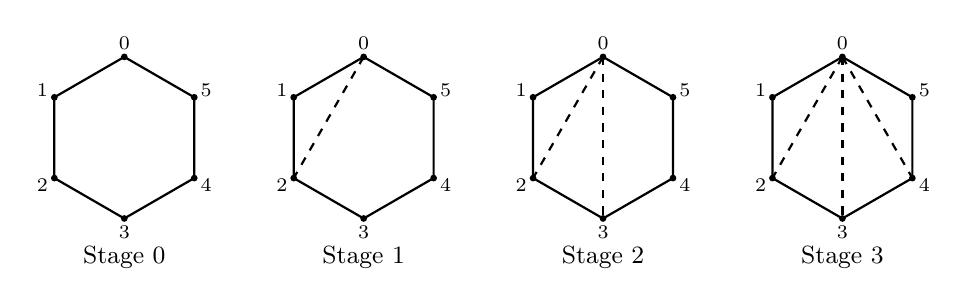
\begin{tikzpicture}[scale=0.76]
\foreach \stage in {0,1,2,3} {
 \begin{scope}[xshift={4.0*\stage cm}]
 \foreach \i in {0,...,5} {\coordinate (p\i) at ({90+60*\i}:1.35);}
 \draw[thick] (p0)--(p1)--(p2)--(p3)--(p4)--(p5)--cycle;
 \ifnum\stage>0 \draw[thick,dashed] (p0)--(p2);\fi
 \ifnum\stage>1 \draw[thick,dashed] (p0)--(p3);\fi
 \ifnum\stage>2 \draw[thick,dashed] (p0)--(p4);\fi
 \foreach \i in {0,...,5} {
  \fill (p\i) circle (1.6pt);
  \node[font=\scriptsize] at ({90+60*\i}:1.58) {$\i$};
 }
 \node[font=\small] at (0,-2.0) {Stage $\stage$};
 \end{scope}
}
\end{tikzpicture}
\caption{Successively introducing three fan diagonals. This regular-hexagon
drawing is a combinatorial schematic; the actual rational coordinates are
$(i,i^2)$, and the heights are~\eqref{poly:ts:eq:hexrows}.}\label{poly:ts:fig:fan}
\end{figure}

The example also distinguishes two tasks. To preserve only the final
triangulation, a single ordinary real height vector is enough. To preserve
all three strict transitions requires three layers. To preserve every
real affine comparison of the original non-Archimedean height vector
requires its full comparison rank. Those numbers agree in this example,
but need not agree in general.
\wtag{} These are three of the invariants compared in
\cref{poly:rem:threedegrees}: the final triangulation (one real vector
here; with a prescribed shadow, degree at most one by \cref{poly:thm:linear}),
the strict geometric history ($r$ layers, \cref{poly:ts:thm:chain}), and the
complete sign type (rank $p=m$, minimum germ degree $m-1$ by
\cref{poly:thm:degree}). \Cref{poly:thm:separation} shows how far apart
they can be.

\section{Shadows and canonical refinement hierarchies}
\label{poly:sec:shadows}

\begin{proposition}[Standard part of a finite convex hull]
\label{poly:prop:stconv}\label{poly:ts:prop:stconv}
For finite points $v_1,\ldots,v_N\in K^D$,
\begin{equation}\label{poly:ts:eq:stconv}
 \st\bigl(\conv_K(v_1,\ldots,v_N)\bigr)
 =\conv_{\R}\bigl(\st(v_1),\ldots,\st(v_N)\bigr).
\end{equation}
\end{proposition}
\begin{proof}
Every convex coefficient lies between zero and one and is therefore
finite. Standard part takes a convex combination to the convex combination
with real coefficients $\st(\lambda_i)$. Conversely every real convex
combination of the shadows is the standard part of the combination of the
original points with those same real coefficients.
\end{proof}
\wtag{} Manuscript~02 proves the same identity (its Proposition ``Standard
part of a finite hull'', for points of $\cO_K^d$) by the same argument; its
labels \texttt{poly:ts:prop:stconv} and \texttt{poly:ts:eq:stconv} are
attached here. \Cref{poly:part:mv,poly:part:ehr,poly:part:ic} use the
identity and cite it here.

The proposition is an equality of convex sets after applying $\st$.
It does not say that standard part sends each face to a face.

\begin{example}[A face whose shadow is not a face]\label{poly:ex:nonface}
Lift the four corners of a unit square with heights $(0,0,0,\eps)$,
where the ordering is $(0,0),(1,0),(0,1),(1,1)$ and $\eps>0$ is
infinitesimal. The first three lifted points form a lower triangular facet.
The shadow of the entire polytope is a square in the plane $z=0$, whereas
the shadow of that facet is the filled triangle with vertices
$(0,0),(1,0),(0,1)$. That triangle is not a face of the square. Thus there
is no unrestricted face-lattice map $F\mapsto\st(F)$.
\end{example}

\begin{proposition}[The shadow subdivision is a coarsening]
\label{poly:prop:refineshadow}
For a bounded lifting of a fixed real base, its marked regular subdivision
refines the one induced by $h^0=\st(h)$: every maximal source cell is
contained in a maximal shadow cell, including inclusion of its contact
labels.
\end{proposition}
\begin{proof}
Choose a supporting basis $B$ of a maximal source cell. All
$s_{B,i}(h)\ge0$, so all
$s_{B,i}(h^0)=\st(s_{B,i}(h))\ge0$. Thus the same basis supports a
shadow cell. Every source equality remains an equality after standard
part, giving $I_B(h)\subseteq I_B(h^0)$.
\end{proof}

More generally the complete flag yields a finite hierarchy, even when the
heights are not bounded. Let $b_1,\ldots,b_m$ be its coefficient rows,
and for $0\le k\le m$ use the lexicographic height with the first $k$
rows. Equivalently take the polynomial
$H_k(t)=\sum_{j=1}^k b_jt^{j-1}$ at a sufficiently small positive real
$t$, with $H_0=0$. Denote its marked subdivision by $\cS_k$.

\begin{proposition}[Canonical finite refinement chain]\label{poly:prop:chain}
The subdivisions $\cS_k$ do not depend on the choice of coefficient
functionals realizing the same oriented flag, and
\[
 \cS_0\succeq\cS_1\succeq\cdots\succeq\cS_m=\cS(h),
\]
where $\succeq$ means ``is coarser than.'' Every subdivision in the chain
is an ordinary real regular subdivision of $A$. There are at most $m$
strict refinement steps. The oriented flag need not be recoverable from
this chain.
\end{proposition}
\begin{proof}
Positive triangular transformations \eqref{poly:eq:triangular} preserve the
first-nonzero signs of every truncated list, so they preserve all truncated
slack signs. Hence the chain depends only on the flag.
If $B$ supports a lower cell for the first $k+1$ rows, every slack has
nonnegative lexicographic sign through that level. Its first $k$ entries
are either all zero or have the same positive first nonzero entry. Thus
$B$ also supports a lower cell at level $k$, and its equality labels can
only increase when the last row is removed. This proves refinement.
Finite sign stabilization realizes every level over $\R$; a common real
parameter can be chosen for the finitely many levels and slacks.

For the last assertion, choose $f_1$ nonzero on every nonzero slack vector
as in Theorem~\ref{poly:thm:separation}. All later rows are invisible to the
subdivision, so $\cS_1=\cdots=\cS_m$ while the remaining flag on
$\ker f_1$ can vary whenever its dimension permits.
\end{proof}

This is a flag-refined version of the usual secondary data, not a claim
that the secondary fan is the entire space of complete dependence types.
Already in a generic real secondary chamber, further infinitesimal
coefficients may encode nontrivial orders on its invisible real dependence
directions.

\section{Standard parts: exact identities and lost faces}\label{poly:ts:sec:standardpart}
\noindent\wtag{} Manuscript~02's standard-part section. Its first
proposition, $\st\conv=\conv\st$, is \cref{poly:prop:stconv} (both sources)
and is not repeated. The finite polar identity, the lost face and the
optimality band are new against 05. Manuscript~05's \cref{poly:ex:nonface}
and 02's \eqref{poly:ts:eq:lostface} are two instances of one failure, a
face whose standard part is not a face; \cref{poly:part:mv} adds a pentagon
(\cref{poly:mv:sec:examples}), and \cref{poly:ts:prop:band} bears on the
questions of \cref{poly:part:mv} about face specialization.

Let $K\supseteq\R$ be an ordered real-closed working field containing a
positive infinitesimal. Write
\[
 \cO_K=\{x\in K:|x|<m\text{ for some }m\in\N\}
\]
for its ring of finite elements. Completeness of $\R$ gives a unique
standard part $\st(x)\in\R$ for each finite $x$: the difference
$x-\st(x)$ is infinitesimal. Standard part is a weakly order-preserving
ring homomorphism on $\cO_K$. Apply it coordinatewise.

\subsection{Convex hull and polar commute with residue}
\noindent\wtag{} The hull identity, 02's first proposition here, is
\cref{poly:ts:prop:stconv}, printed once above for both sources.

\begin{proposition}[Finite polar residue]\label{poly:ts:prop:polar}
Let $P=\conv_K(v_1,\ldots,v_n)$ with all $v_i$ finite, and define
$P^\circ=\{y\in K^d:y\cdot x\le1\text{ for all }x\in P\}$.
No assumption that $0$ is interior is required. Then
\begin{equation}\label{poly:ts:eq:polar}
 \st(P^\circ\cap\cO_K^d)=(\st P)^\circ.
\end{equation}
\end{proposition}
\begin{proof}
If $y$ is a finite polar point, standard part of each inequality
$y\cdot v_i\le1$ gives the inclusion from left to right. For the reverse
inclusion, let $y\in(\st P)^\circ\subseteq\R^d$ and put
\[
 \delta=\max\bigl(0,\max_i(y\cdot v_i-1)\bigr).
\]
All terms are finite and their standard parts are nonpositive, so
$\delta$ is a nonnegative infinitesimal. The point
$y'=y/(1+\delta)$ satisfies $y'\cdot v_i\le1$ for all $i$, is finite,
and has standard part $y$. Thus $y'\in P^\circ\cap\cO_K^d$.
\end{proof}

The finite-part restriction in~\eqref{poly:ts:eq:polar} matters because a polar
can be unbounded and standard part is not defined on infinite coordinates.
The proof does not need a Hausdorff convergence theorem or a metric on
all of $K^d$.

\subsection{A face need not have a face as its standard part}
Consider
\begin{equation}\label{poly:ts:eq:lostface}
 P=\conv_K\{(-1,0),(0,-\eps),(1,0),(1,1),(-1,1)\}.
\end{equation}
Its unique point maximizing $(x,y)\mapsto-y$ is the vertex $(0,-\eps)$.
The standard-part hull is the rectangle
$Q=[-1,1]\times[0,1]$. The standard part of that vertex is $(0,0)$,
which lies in the relative interior of the bottom edge of $Q$ and is not
a face by itself.

Thus the assignment $F\mapsto\st(F)$ is not a map from the face lattice
of $P$ to the face lattice of $Q$. This is stronger than the observation
that two vertices can merge. Even an exposed face can map to a proper
nonface subset of a limiting face.

\subsection{Near-optimal points recover the lost limiting face}
\begin{proposition}[An exact infinitesimal optimality band]\label{poly:ts:prop:band}
Let $P=\conv_K(v_1,\ldots,v_n)$ be finite, $Q=\st(P)$, and
$c\in\R^d$. Put $M=\max_i c\cdot v_i$ and $m=\st(M)$. There is a
positive infinitesimal $\eta$ such that
\begin{equation}\label{poly:ts:eq:band}
 \st\{x\in P:c\cdot x\ge M-\eta\}
 =\argmax_{y\in Q}c\cdot y.
\end{equation}
\end{proposition}
\begin{proof}
Standard part commutes with a finite maximum, so
$m=\max_{y\in Q}c\cdot y$. Let
\[
 J=\{i:c\cdot\st(v_i)=m\},\qquad
 D=\max_{i\in J}(M-c\cdot v_i).
\]
The set $J$ is nonempty, and $D$ is a nonnegative infinitesimal. Choose
any positive infinitesimal $e\in K$ and set $\eta=D+e$.

A point in the band on the left of~\eqref{poly:ts:eq:band} has standard-part
objective value at least $m$, hence exactly $m$ because its standard
part lies in $Q$. Conversely, every $v_i$ with $i\in J$ belongs to the
band, and so does their $K$-convex hull. Its standard part is the real
convex hull of the maximizing standard-part vertices. That is the entire
maximizer face of $Q$, proving the other inclusion.
\end{proof}

For~\eqref{poly:ts:eq:lostface}, exact optimization remembers just the infinitesimally
lower vertex, but an appropriate infinitesimal optimality band recovers
the whole bottom edge. This suggests that residue geometry should retain
near-optimal fibers or scale-decorated cells rather than attempt to force
a false homomorphism between ordinary face lattices.

\section{Higher-rank tropical minimizers: an elementary bridge}
\label{poly:sec:tropical}

This section records a finite-rank interpretation of the hierarchy, not a
new theory of higher-rank tropical multiplicities. It is useful for comparing
the lifting package with \cite{fs:JS,fs:CCFL} without identifying different
notions of topology or convexity.

Take real height rows $b_1,\ldots,b_r\in\R^n$. For
$x=(x_1,\ldots,x_r)\in(\R^d)^r$, compare the vectors
\[
 \Phi_i(x)=
 (b_{1,i}+a_i\cdot x_1,\ldots,b_{r,i}+a_i\cdot x_r)
 \in\R^r
\]
in lexicographic order. Define $I_0=\{1,\ldots,n\}$ and successively
\begin{equation}\label{poly:eq:nestedmin}
 I_j(x)=\operatorname*{arg\,min}_{i\in I_{j-1}(x)}
                 (b_{j,i}+a_i\cdot x_j).
\end{equation}
The final minimizers of $\Phi_i(x)$ are exactly $I_r(x)$.

For nonempty $T\subseteq S\subseteq\{1,\ldots,n\}$ set
\[
 \cD_b^S(T)=\{y\in\R^d:
       \operatorname*{arg\,min}_{i\in S}(b_i+a_i\cdot y)=T\}.
\]
This is a relatively open polyhedron, possibly empty. Indeed choose
$i_0\in T$, impose equalities
\[
 (a_i-a_{i_0})\cdot y=b_{i_0}-b_i\quad(i\in T),
\]
and strict inequalities saying that every $i\in S\setminus T$ has a
larger value. If nonempty, it has dimension $d-\dim\aff(A_T)$.

\begin{proposition}[Product strata for a fixed minimizer history]
\label{poly:prop:tropstrata}
For a specified chain of nonempty sets
$I_0\supseteq I_1\supseteq\cdots\supseteq I_r$, the points $x$ with
this exact successive minimizer history form
\begin{equation}\label{poly:eq:productstrata}
 \cD_{b_1}^{I_0}(I_1)\times
 \cD_{b_2}^{I_1}(I_2)\times\cdots\times
 \cD_{b_r}^{I_{r-1}}(I_r).
\end{equation}
A nonempty such stratum has dimension
\[
 rd-\sum_{j=1}^r\dim\aff(A_{I_j}).
\]
There are finitely many histories, and the lexicographic tie locus is the
disjoint union of those strata with $|I_r|\ge2$.
\end{proposition}
\begin{proof}
Lexicographic comparison first discards all labels not minimizing the first
coordinate, then discards nonminimizers of the second among the survivors,
and continues. For a prescribed chain, the $j$th condition involves only
$x_j$, which proves the product formula. The equalities defining a
nonempty factor have rank $\dim\aff(A_{I_j})$. Its strict inequalities
cut out an open subset of that affine solution space and do not decrease
its dimension. Dimensions add under products. The finiteness and disjointness
follow because every $x$ has a unique chain of finite sets.
\end{proof}

This derivation makes no claim that the Euclidean closures of these strata
constitute a pure polyhedral complex. Higher-rank examples can fail the
naive closure and purity expectations; such issues are treated explicitly
in \cite{fs:JS}. Its rank-two product decomposition is a close precedent for
\eqref{poly:eq:productstrata}. The newer framework \cite{fs:CCFL} uses higher-rank
GKZ cones and its own face and coface structure. A scalar-field Farkas
lemma over $K$ and a separation statement for lexicographically ordered
matrix halfspaces are different assertions; one cannot import one as the
other without checking the ambient structure.

The present finite compression concerns the \emph{height dependence
space}. It does not preserve the full ordered multiplicative group of all
surreal monomials. Nor does it supply tropical weights, balancing, or the
algebraic degeneration machinery of \cite{fs:CCFL}. Those are additional
structures beyond the sign and leading-term invariants proved here.

\section{Examples that locate the exact boundary}
\label{poly:sec:examples}

\subsection{Identical leading heights, opposite square diagonals}

For the square ordered as above, the affine-dependence space is spanned by
$c=(1,-1,-1,1)$. Consider
\[
 h^+=(1,1,1,1+\eps),\qquad h^-=(1,1,1,1-\eps),
 \qquad 0<\eps\ll1.
\]
All four individual heights have leading term $1$ in both liftings and
both standard parts are $(1,1,1,1)$. Yet
\[
 L_{h^+}(c)=\eps,\qquad L_{h^-}(c)=-\eps.
\]
The positive case uses diagonal $a_2a_3$, with maximal cells
$\{1,2,3\}$ and $\{2,3,4\}$. The negative case uses diagonal $a_1a_4$,
with maximal cells $\{1,2,4\}$ and $\{1,3,4\}$. These exact contact-label
sets are also returned by the supplied checker.

\begin{figure}[ht]
\centering
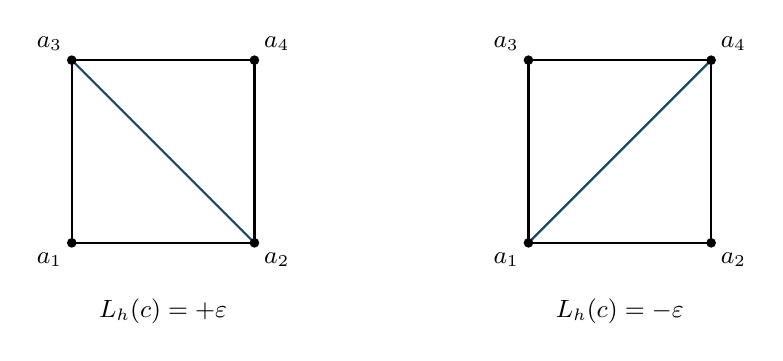
\begin{tikzpicture}[scale=1.45,every node/.style={font=\small}]
 \begin{scope}
 \draw[thick] (0,0)--(1.6,0)--(1.6,1.6)--(0,1.6)--cycle;
 \draw[thick,inkblue] (1.6,0)--(0,1.6);
 \foreach \x/\y/\n in {0/0/1,1.6/0/2,0/1.6/3,1.6/1.6/4}
   {\fill (\x,\y) circle (1.2pt);}
 \node[below left] at (0,0) {$a_1$};\node[below right] at (1.6,0) {$a_2$};
 \node[above left] at (0,1.6) {$a_3$};\node[above right] at (1.6,1.6) {$a_4$};
 \node at (.8,-.6) {$L_h(c)=+\eps$};
 \end{scope}
 \begin{scope}[xshift=4cm]
 \draw[thick] (0,0)--(1.6,0)--(1.6,1.6)--(0,1.6)--cycle;
 \draw[thick,inkblue] (0,0)--(1.6,1.6);
 \foreach \x/\y/\n in {0/0/1,1.6/0/2,0/1.6/3,1.6/1.6/4}
   {\fill (\x,\y) circle (1.2pt);}
 \node[below left] at (0,0) {$a_1$};\node[below right] at (1.6,0) {$a_2$};
 \node[above left] at (0,1.6) {$a_3$};\node[above right] at (1.6,1.6) {$a_4$};
 \node at (.8,-.6) {$L_h(c)=-\eps$};
 \end{scope}
\end{tikzpicture}
\caption{The coordinatewise leading heights and the real shadows agree;
 the first nonzero affine-dependence coefficient determines different
 regular triangulations. The figure shows the projected lower cells.}
\end{figure}

\subsection{A nontrivial three-scale compression}

Take $A=(0,1,2,3,4)$ in one dimension, and gauge the first two heights to
zero. On the last three coordinates put
\begin{align*}
 g={}&(1,1,0)\eps+(2,2,0)\eps^2+(0,1,1)\eps^5\\
    &+(1,-2,-3)\eps^6+(1,0,1)\eps^9,
 \qquad \eps=\omega^{-1}.
\end{align*}
The coefficient at $\eps^2$ is twice the first; the coefficient at
$\eps^6$ is $(1,1,0)-3(0,1,1)$. The coefficient-pivot procedure therefore
selects powers $1,5,9$, and
\[
 g^\sharp=(1,1,0)\eps+(0,1,1)\eps^5+(1,0,1)\eps^9.
\]
The three selected rows are independent. Every real linear combination
of the three original coordinates has exactly the same leading term after
compression, not merely the same sign on the finitely many circuits.
A shadow-preserving polynomial model is
\[
 H(t)=(0,0,t+t^3,t+t^2,t^2+t^3).
\]
Its minimum degree for the complete sign type with zero shadow is three.
The exact checker gives the sufficient bound $\eta_0=1/10$, the sample
$t_0=1/20$, and lower maximal contact sets $\{1,2\}$ and $\{2,5\}$.
Thus a degree-one path from zero to $H(1/20)$ already retains the finite
lifted geometry, while losing some of the full real dependence type.

The gaps between the powers could be replaced by much larger surreal
exponent gaps. The proof depends on their order and coefficient spans,
not on the existence of a smallest step in the exponent group.

\subsection{Unsigned determinant valuations also lose combinatorics}

Let $\delta>0$ be infinitesimal and $u=(1,1)$. For a real configuration
$A$ put $p_i=u+\delta a_i$. Every coordinate of every $p_i$ has leading
term $1$. Every nonzero augmented $3\times3$ determinant is
$\delta^2$ times the corresponding real determinant. Compare
\[
 A=\{(0,0),(2,0),(0,2),(2,2)\}
\]
with
\[
 A'=\{(0,0),(2,0),(0,2),(1/2,1/2)\}.
\]
In both configurations every triple is affinely independent, so all these
determinants have the same leading exponent. Nevertheless one hull has
four vertices and the other has three, with a labeled interior point.
Neither coordinate leading terms nor the unsigned determinant valuations
recover the labeled face lattice. The signs of leading coefficients matter.

\subsection{Finite truncation can destroy an exact equality}\label{poly:sec:truncation}

Let $y=\eps$ and $x=\eps+\eps^2+\cdots=\eps/(1-\eps)$.
The exact algebraic relation $(1-y)x-y=0$ holds. Replacing $x$ by the
first $N$ terms gives
\[
 (1-\eps)(\eps+\cdots+\eps^N)-\eps=-\eps^{N+1}\ne0.
\]
The pivot theorem preserves real \emph{linear} combinations. It does not
preserve arbitrary polynomial relations between the coordinates, and it
must not be advertised as a finite truncation algorithm for a surreal field.

\subsection{One parameter does not preserve the entire scale field}\label{poly:sec:oneparam}

The positive infinitesimals
$\eps=\omega^{-1}$ and $\tau=\omega^{-\omega}$ satisfy
$\tau<\eps^N$ for every positive ordinary integer $N$. Replacing them
by $t^a,t^b$ with fixed positive real $a,b$ in a rank-one monomial group
cannot preserve all these inequalities: choose $N>b/a$. Our finite-height
models preserve a specified real-linear dependence type, not every
multiplicative comparison in the field generated by the original scales.
This is a boundary on what the theorem says, not a contradiction to its
polynomial realization conclusion.

\section{A toric application: preserving the whole initial ideal}
\label{poly:sec:toric}

Suppose now that the base points are integral, $a_i\in\Z^d$, and let
$k$ be any field. The homogeneous toric ideal is
\[
 I_A=\ker\bigl(k[x_1,\ldots,x_n]\longrightarrow
                 k[z_0,z_1^{\pm1},\ldots,z_d^{\pm1}],
                 \quad x_i\longmapsto z_0z^{a_i}\bigr).
\]
For a polynomial, define its $h$-initial form to be the sum of the terms
whose weights $\sum_i u_i h_i$ are \emph{maximal}. These weights lie in
the ordered additive group of $\No$; no infinite sum or coefficient
valuation is involved. The ideal generated by the initial forms of all
members of $I_A$ is denoted $\operatorname{in}_h I_A$.

Put $\Lambda=\ker_{\Z}\Atil$. For $c\in\Lambda$ write
$c=c^+-c^-$ with disjoint nonnegative integer supports, and set
$B_c=x^{c^+}-x^{c^-}$. Its initial form depends only on $\chi_h(c)$.
A vector $g\in\Lambda\setminus\{0\}$ is \emph{conformally indecomposable}
when it is not a sum of two nonzero lattice vectors lying in its closed
orthant, with their absolute values adding coordinatewise. The set $G_A$
of these vectors, with either both signs or one representative of each
pair, is the Graver basis. Its relationship with universal Gr\"obner
bases is classical; see, for example, \cite{fs:Petrovic}. We include the
finite argument needed for arbitrary ordered weights.

\begin{lemma}[A finite certificate for arbitrary ordered weights]
\label{poly:lem:graver}
The set $G_A$ is finite. For heights in any totally ordered abelian group,
\[
 \operatorname{in}_h I_A
 =\bigl\langle\operatorname{in}_h B_g:g\in G_A\bigr\rangle.
\]
\end{lemma}
\begin{proof}
In each orthant, conformal indecomposables are the minimal nonzero elements
of the lattice under coordinatewise comparison of absolute values.
Dickson's lemma makes this set finite. One proof of that lemma is induction
on the number of coordinates: any infinite sequence in $\mathbb N^n$
contains an infinite subsequence whose first coordinate is nondecreasing;
apply the induction hypothesis to the remaining coordinates to find a
comparable pair. An infinite set of distinct minimal elements would give
an infinite sequence with no such pair.

Repeatedly splitting a decomposable lattice vector strictly decreases the
positive integer $\ell^1$-size of each resulting summand. Thus every
$c\in\Lambda\setminus\{0\}$ has a conformal decomposition
$c=g_1+\cdots+g_s$ into Graver vectors. Let
$\alpha_j=h\cdot g_j$. If $h\cdot c>0$, then some $\alpha_j>0$.
The monomial $\operatorname{in}_h B_{g_j}=x^{g_j^+}$ divides
$x^{c^+}=\operatorname{in}_h B_c$. The negative case is symmetric.
If $h\cdot c=0$ and not all $\alpha_j$ vanish, there are both a
positive and a negative $\alpha_j$. The two terms of $B_c$ are then
separately divisible by initial monomials of Graver binomials.
If all $\alpha_j=0$, use the identity, valid for conformal sums,
\[
 B_{g+g'}=x^{g'^+}B_g+x^{g^-}B_{g'}.
\]
It expresses $B_c$ in the ideal generated by the tied Graver binomials.
Hence every initial form of a lattice binomial belongs to the stated ideal.
A common monomial factor handles binomials whose exponents overlap.

It remains to justify that binomials suffice. Decompose any $f\in I_A$
into its $\Atil$-homogeneous parts. Within each part, the coefficients sum
to zero, because all monomials have the same image under the toric map.
If the terms of one part have different weights, every maximal-weight
monomial is the initial monomial of its difference with a lower-weight
monomial in that same part. If all its terms have equal weight, the whole
part is a linear combination of tied differences with one fixed monomial.
Thus its initial form belongs to the ideal of initial binomials. The
initial form of the original $f$ is a sum of the initial forms of those
homogeneous parts whose maximal weights attain the global maximum, so
it belongs as well. The reverse inclusion follows because every $B_g$
belongs to $I_A$.
\end{proof}

\begin{theorem}[Toric compatibility of compression and real shadows]
\label{poly:thm:toric}
For an integral base configuration, the compressed lifting satisfies
\[
 \operatorname{in}_{h^\sharp}I_A=\operatorname{in}_h I_A.
\]
A polynomial model of its complete dependence type has the same initial
ideal for every sufficiently small positive real parameter. If $h$ is
bounded, a real affine-linear path starting at $\st(h)$ can preserve this
initial ideal, all the lifted determinant signs, and the marked lower
subdivision simultaneously on its whole punctured segment.
\end{theorem}
\begin{proof}
Compression preserves the sign of $L_h(g)$ for every $g\in G_A\subseteq V$,
so Lemma~\ref{poly:lem:graver} gives the first equality. The finite sign lemma
applied to these Graver comparisons proves stabilization along a polynomial
model. For the last assertion, add $G_A$ to the finite determinant and
slack test list in Theorem~\ref{poly:thm:linear}.
\end{proof}

This preserves the initial ideal itself, not only its radical or the
underlying subdivision. The initial algebra and its scheme-theoretic
invariants therefore agree. The statement is an application of classical
finite Graver control together with our lifting construction; it is not a
new construction of the higher-rank degenerations of \cite{fs:CCFL}.
For the square, $I_A=(x_1x_4-x_2x_3)$: the two infinitesimal choices above
give initial ideals $(x_1x_4)$ and $(x_2x_3)$, respectively.

\section{General surreal polytopes: what transfer gives and what it does not}
\label{poly:sec:general}\label{poly:ts:sec:transfer}

\begin{theorem}[Classical finite realization and shadow arcs]
\label{poly:thm:general}\label{poly:ts:thm:transfer}
Every finite surreal point configuration has the same labeled oriented
matroid, and hence the same labeled polytope face structure, as a real
configuration. Without prescribed real coordinates or other real
parameters, a realization can be chosen with real algebraic coordinates.
If the original coordinates are finite, there is a real semialgebraic arc
of configurations with the same finite determinant signs that converges
to their labeled standard parts. Additional \emph{finitely many} polynomial
sign conditions can be preserved along the same arc.
\wtag{} In manuscript~02's form (its Theorem ``Classical real-algebraic
transfer''): for any finite labeled configuration $V=(v_1,\ldots,v_n)$ in a
real-closed field, there is a labeled configuration of real algebraic points
with the same signed affine-hyperplane patterns and the same affine
dimension. In particular, the two convex hulls have isomorphic labeled face
lattices.
\end{theorem}
\begin{proof}
List the signs of all minors of the homogeneous coordinate matrix, keeping
each zero as an equality. This is a finite system of polynomial equalities
and strict inequalities with integer coefficients. It has a solution in
a set-sized real closed subfield of $\No$ containing the coordinates.
Completeness of the theory of real closed fields transfers the existential
sentence to $\R$, and also to the real algebraic numbers when there are
no prescribed real parameters. The minor signs determine the rank and
oriented matroid; the facet reconstruction in
Lemma~\ref{poly:lem:faces}, in its appropriate affine rank, gives the face
structure. These are standard real-algebraic facts \cite{fs:BPR}.

For the bounded assertion, let $v^0$ be the vector of all standard-part
coordinates and let $S$ be the corresponding real semialgebraic sign cell,
including the extra predicates when present. For every positive real
$r$, the surreal tuple lies in the ball of radius $r$ about $v^0$ and
satisfies the sign conditions. Transfer over the named real parameters
shows that $S$ contains a real tuple within that ball. Thus
$v^0\in\overline S$. If a constant configuration already suffices, take
a constant arc. Otherwise semialgebraic curve selection yields an arc
entering $S$ and tending to $v^0$ \cite{fs:BPR,fs:BR}. Its one-variable
semialgebraic coordinates are algebraic-function branches; one may use
a finite power reparameterization to obtain analytic branches at the
endpoint. The determinant signs on the punctured arc are the desired ones.
\end{proof}
\begin{proof}[Second proof of the realization assertion, in manuscript 02's covector form (source 02)]
For each $\sigma\in\{-1,0,1\}^n$, let $\Psi_\sigma(V)$ be the formula
\[
 \exists u_1,\ldots,u_d,b\quad
 \bigwedge_{i=1}^n
 \sgn(u\cdot v_i+b)=\sigma_i.
\]
Replace each sign assertion by the corresponding polynomial equality or
strict inequality. There are only $3^n$ patterns. Conjoin $\Psi_\sigma$ for
all patterns realized by $V$ and $\neg\Psi_\sigma$ for all other patterns.
Also conjoin the finite minor conditions expressing its affine dimension.
Finally existentially quantify the coordinates of $V$.

The resulting sentence is a first-order sentence of ordered rings with
integer coefficients. It is true in the given real-closed field. By the
completeness of the theory of real-closed fields, equivalently by Tarski's
elimination theorem~\cite{ts:vdD}, it is true in the real algebraic numbers,
which themselves form a real-closed field. Choose a witnessing configuration
there.

A supporting affine functional has all its values nonpositive after
subtracting its maximum. Its zero labels are exactly the labels on its
maximizing face. Thus the all-nonpositive sign patterns recover all
nonempty face label sets; adding the empty face gives the entire labeled
face lattice. The construction preserves these patterns and their
inclusions.
\end{proof}

\noindent\wtag{} The next two paragraphs follow the transfer theorem in
manuscript~02; the family announced at their end is the lifting compression
of \cref{poly:ts:sec:compression}.\par
This theorem is intentionally stronger than a statement about the numbers
of faces: it preserves the entire affine covector system. It is also
intentionally weaker than an exact coordinate representation. There is no
order-preserving field map from $\No$ into $\R$ fixing $\R$, since a positive
infinitesimal would have to become a positive real number smaller than every
$1/m$. Nor does the theorem guarantee rational coordinates.

Consequently, such familiar finite combinatorial questions as which
$f$-vectors occur do not acquire additional examples merely by allowing
surreal coordinates. Any genuinely additional information must reside in
scales, residue maps, simultaneous structures, or infinite families of
observations. We turn to one such family.


The realization statement is classical transfer, not a new surreal
realizability theorem. Likewise the general arc existence is an application
of curve selection; \cite{fs:BR} supplies a quantitative framework. The
special contribution of the fixed-base setting is the elementary
polynomial model with sharp degree and the linear finite-data path.

\begin{example}[Polynomial arcs need not preserve nonlinear constraints]
Take the finite surreal point
\[
 (x,y)=\bigl(\sqrt{1-\eps^2},\eps\bigr),\qquad 0<\eps\ll1.
\]
It lies on the unit circle, has $y>0$, and has standard part $(1,0)$.
There is no real polynomial arc $(X(t),Y(t))$ with
$(X(0),Y(0))=(1,0)$, $X(t)^2+Y(t)^2=1$, and $Y(t)>0$ for small positive
$t$. Indeed, if either polynomial is nonconstant, the coefficient of the
largest even degree in $X^2+Y^2$ is a positive sum of squares and cannot
vanish. Both must therefore be constant, contradicting the endpoint and
$Y(t)>0$. An algebraic analytic arc exists, but a polynomial one does not.
This example concerns the permitted extra polynomial constraints; it is
not claimed as an obstruction arising from determinant signs alone.
\end{example}

\section{A finite Puiseux model with the same residue}\label{poly:ts:sec:puiseux}
\noindent\wtag{} \Cref{poly:ts:thm:puiseux} is the bounded half of
\cref{poly:thm:general} (source~05) in manuscript~02's form: it keeps the
full signed affine-hyperplane patterns and any finite list of real polynomial
signs along a semialgebraic arc starting at the standard part, with
convergent algebraic Puiseux germs. Both proofs are the same
transfer-and-curve-selection argument (05 cites
\cite{fs:BPR,fs:BR}, 02 cites \cite{ts:BCR,fs:BR}). The circle example after
\cref{poly:thm:general} shows that such arcs cannot in general be taken
polynomial. The finite-support specialization \cref{poly:mv:thm:compression}
of \cref{poly:part:mv} is an effective counterpart for finite-support
Hahn certificates.

The universal truncation theorem does not prevent a \emph{different}
well-chosen real one-parameter model from preserving any finite collection
of incidence data. This is a useful distinction between an arbitrary
coordinate truncation and a controlled semialgebraic specialization.

\begin{theorem}[Finite incidence-and-residue realization]\label{poly:ts:thm:puiseux}
Let $V\in\cO_K^{dn}$ be a finite bounded configuration and let
$b=\st(V)\in\R^{dn}$. Fix any finite collection of polynomials with real
coefficients in the coordinates of $V$. There is a continuous
semialgebraic arc $\gamma:[0,a)\to\R^{dn}$ such that
\begin{enumerate}[label=(\alph*)]
\item $\gamma(0)=b$;
\item for every sufficiently small $s>0$, all the prescribed polynomial
signs at $\gamma(s)$ equal those at $V$;
\item for those $s$, the configuration $\gamma(s)$ has the same signed
affine-hyperplane patterns and affine dimension as $V$.
\end{enumerate}
The coordinate germs of $\gamma$ can be taken to be convergent algebraic
Puiseux germs over $\R(s)$. In particular, they give a finite geometric
model with the full face lattice of $V$ and its prescribed standard-part
limit.
\end{theorem}
\begin{proof}
Encode the prescribed polynomial signs and the complete finite list of
affine sign patterns exactly as in Theorem~\ref{poly:ts:thm:transfer}, now keeping
real parameters. Include the rank conditions. Quantifier elimination makes
the resulting condition a semialgebraic set $S\subseteq\R^{dn}$, and the
original configuration satisfies the same defining condition in $K$.

For every real $\delta>0$, the field $K$ satisfies
\[
 \exists z\in S(K)\quad \max_i|z_i-b_i|<\delta,
\]
since $z=V$ is a witness. The inclusion $\R\subseteq K$ is elementary
for ordered-ring formulas, by real-closed-field quantifier elimination.
Hence the displayed assertion has a real witness. It follows that
$b\in\overline S$ in the ordinary Euclidean topology.

If $b\in S$, the constant arc is sufficient. Otherwise apply the
semialgebraic curve selection lemma to $S$ at $b$. It gives a continuous
semialgebraic arc with initial point $b$ and positive-time values in $S$.
This proves (a)--(c). A one-variable semialgebraic function has, after
restricting to a sufficiently short interval, an algebraic Puiseux germ;
its Puiseux expansion is convergent. Equivalently, after a common finite
ramification $s=u^m$, all the coordinate germs are analytic at the
endpoint. These are the standard curve-selection and algebraic-Puiseux
facts from real algebraic geometry~\cite{ts:BCR,fs:BR}.
\end{proof}

Here ``algebraic'' means algebraic over $\R(s)$, not that every coefficient
is a real algebraic number. The limiting configuration may itself contain
transcendental real coordinates. Theorem~\ref{poly:ts:thm:puiseux} is a synthesis
of standard transfer and curve-selection tools, not a new curve selection
lemma. It supplies neither explicit complexity bounds nor a coordinate
embedding of the original surreal field.

Most importantly, its quantifier is \emph{finite}. The chosen arc can
preserve the final four-point hull and its residue, or any finite list of
additional polynomial observations. It need not preserve the arbitrary
infinite sequence of coordinate-truncation hulls constructed in
Section~\ref{poly:ts:sec:universal}. This is exactly how finite realizability and
infinite scale complexity coexist.

\section{Corrections to the earlier convexity draft}
\label{poly:sec:corrections}
\noindent[\textup{[write]} The draft corrected here, \emph{Finite Convexity and Exact Lexicographic Optimization over the Surreals} (22~September 2026), was supplied privately to the authors of manuscripts 05 and 07; it is not part of ProveIt and could not be checked. The statements below are printed as standalone results.]

The earlier draft \cite{fs:PriorDraft} contains a valid sufficiently-small
comparison argument. Its Proposition 7.1, however, identifies the
\emph{entire} positive validity set with an interval. Its Theorem 9.1 and
following explanation also require a distinction between a real domain
and its scalar extension. Neither issue affects the proofs above.

\subsection{The global validity set need not be an interval}

On $P=[0,1]$, take the objective hierarchy
$c_0x=x$, $c_1x=-3x$, and $c_2x=2x$. Lexicographic maximization selects
$x=1$. The compiled objective is
\[
 (1-3t+2t^2)x=(1-t)(1-2t)x.
\]
It selects exactly the same maximizer for
\begin{equation}\label{poly:eq:reentry}
 t\in(0,1/2)\ \cup\ (1,\infty),
\end{equation}
not for a single interval. At $t=1/2$ and $t=1$ it is constant on the
whole segment; between those points it selects $x=0$.

\begin{proposition}[Correct initial-radius statement]\label{poly:prop:radius}
For finitely many nonzero comparison polynomials with their required
signs at $0^+$, the component of the simultaneous validity set adjacent
to zero is $(0,\rho)$, where $\rho$ is the least positive zero of one
of the normalized nonzero comparison polynomials, or $+\infty$ when
none has a positive zero. Over a real closed coefficient field, a finite
$\rho$ belongs to that field. The entire validity set may have additional
components beyond $\rho$.
\end{proposition}
\begin{proof}
Divide each polynomial by its lowest power of $t$; its constant term is
nonzero. Before its first positive zero its sign is constant, by the
intermediate value property. At a positive zero the required strict sign
fails, even if the polynomial merely touches zero and later has the same
sign again. Taking the least positive zero over the finite list gives
exactly the component adjacent to zero. Signs on subsequent root intervals
can agree again, as \eqref{poly:eq:reentry} shows.
\end{proof}

For a general ordered field the first zero may lie only in a real closure,
so the endpoint may define a cut rather than an element of the original
field. A sufficient algebraic bound such as Lemma~\ref{poly:lem:eta} avoids
this issue. We never use a global-interval assertion.

\subsection{A real face and its scalar extension are different sets}

Let $P_{\R}=\conv_{\R}(v_1,\ldots,v_N)$ with real vertices, and let
$P_K=\conv_K(v_1,\ldots,v_N)$. Suppose a compiled objective makes exactly
the labels in $J$ optimal. Then
\begin{equation}\label{poly:eq:facebasechange}
 \operatorname*{arg\,max}_{x\in P_K}c\cdot x
   =\conv_K\{v_j:j\in J\},
\end{equation}
not generally $\conv_{\R}\{v_j:j\in J\}$.
To prove \eqref{poly:eq:facebasechange}, express $x$ as a convex combination
and subtract its objective value from the optimal vertex value. The result
is a sum of nonnegative terms. Equality forces every positive coefficient
to occur at an optimal vertex, exactly as over $\R$.

For example, maximizing the first coordinate on $[0,1]^2_K$ gives the
whole edge $\{1\}\times[0,1]_K$, including $(1,\eps)$ for a positive
infinitesimal $\eps\in K$. This point is not in the ordinary real edge.
The correct shadow identity is
\[
 \st\!\left(\operatorname*{arg\,max}_{P_K}c\cdot x\right)
   =\conv_{\R}\{v_j:j\in J\},
\]
by Proposition~\ref{poly:prop:stconv}. The same optimal \emph{vertex labels}
and the same base-changed face are selected. If the old statement is read
literally with optimization only over the subset $P_{\R}\subset\No^d$,
then equality with the real face is correct; it is not the assertion about
$K$-convex polytopes used elsewhere. This is a scalar-extension ambiguity,
not a reason to discard the finite compiler.

\section{Computation, certificates, and a formalization route}
\label{poly:sec:computation}

\subsection{What the executable verifier actually does}

The accompanying \nolinkurl{code/05-finite-scale-liftings-verify.py} \wtag{} (delivered as \nolinkurl{code/verify.py}) uses only Python's standard
library and exact rational arithmetic. It accepts the finite examples
encoded there as Laurent polynomials in a positive infinitesimal
$\eps=\omega^{-1}$. An input coefficient list is complete, not an oracle
that may reveal further terms later. The procedure is:
\begin{enumerate}[label=\arabic*.]
\item find affine bases by exact determinants and compute barycentric
      coefficients by exact elimination;
\item subtract the affine gauge coefficientwise and retain exactly the
      rank-increasing coefficient rows;
\item build the polynomial model, every affine-basis slack, and every
      augmented maximal minor;
\item compare leading terms and signs before and after compression,
      compute the rational threshold, and verify the real specialization
      and several points on the linear shadow path.
\end{enumerate}
The theorem proves validity on the whole segment; the sampled points are
only additional implementation checks. Exact leading-term equality is
checked on the finite determinant/slack list and on 60 additional rational
dependence vectors per example. No finite test can replace the universal
proof in Theorem~\ref{poly:thm:pivot}.

The executed suite contains seven named cases, six members of the sharpness
family, and forty randomized rational configurations using seed
\texttt{20260930}. All fifty-three cases passed, including the three-scale pivot
list $[1,5,9]$ and the validity-set counterexample. This gives 3,180 extra
sampled dependence checks, in addition to the complete finite geometry
test lists for each case. Machine-readable data are in
\nolinkurl{data/05-finite-scale-liftings-certificates.json}; the execution summary is in
\nolinkurl{data/05-finite-scale-liftings-verification_report.txt}. The program does not implement
arbitrary surreal arithmetic, semialgebraic curve selection, or a Graver
basis algorithm. The corresponding general results rest on the written
proofs, not on a claimed implementation.

If the finite support has $s$ coefficient rows and the affine-dependence
dimension is $q$, an incremental elimination implementation can perform
the pivot selection using $O(sq^2)$ field operations, after gauging.
The supplied reference verifier recomputes some small ranks for simplicity;
it is not presented as achieving that optimized complexity. Enumerating
all affine bases involves at most $\binom{n}{d+1}$ candidates, and rational
bit growth must be accounted for in any bit-complexity claim.

\subsection{Why coefficient access alone does not make the bound computable}

\begin{proposition}[An explicit representation obstruction]
\label{poly:prop:undecidable}
There is no algorithm that always computes $m$ for rational-coefficient
height series given by uniformly computable coefficient functions, even
under the promise that each series actually has finite support and that
the real base configuration is fixed.
\end{proposition}
\begin{proof}
Use $A=(0,1,2,3)$ and gauge the first two heights to zero. For a Turing
machine $e$, let $x_e=\eps^{T+1}$ if it halts for the first time at step
$T$, and let $x_e=0$ if it never halts. The coefficient of $\eps^N$ in
$x_e$ is computable uniformly from $e,N$ by simulating at most $N$ steps.
Every resulting series has at most one nonzero coefficient. Take heights
$(0,0,1,x_e)$. Their dependence-image dimension is one if the machine
never halts and two if it halts, since a nonzero positive infinitesimal is
real-linearly independent of $1$. An algorithm computing $m$ from these
coefficient functions would decide the halting problem.
\end{proof}

Thus a complete finite support list and a computable coefficient function
with a finite-support promise are very different input representations.
The latter supplies no computable bound on the last possible nonzero
coefficient. The rank theorem does not erase that distinction.

\subsection{A finite certificate workflow}\label{poly:ts:sec:workflow}
\noindent\wtag{} This subsection and the next are from manuscript~02's
section ``Algorithms, verification, and proof boundaries''
(\cref{poly:ts:sec:verification} prints the rest). Its query-model bound
\cref{poly:ts:prop:oracle} and 05's \cref{poly:prop:undecidable} are
different obstructions and both are kept: 02's is an adversary argument in
the query model (no algorithm that halts after finitely many coefficient
queries computes the rank of every finite-support input), 05's a reduction
of the halting problem for uniformly computable coefficient functions.
For a real base with a supplied finite rational array of height
coefficients, the positive results suggest the following reproducible
workflow. Compute affine bases and their barycentric slack vectors. Fix
one basis to gauge away affine coefficient rows by~\eqref{poly:ts:eq:gauge}.
Scan the ordered row array, retaining each rank-increasing residual row.
For every retained prefix, enumerate lower bases by lexicographic slack
signs and deduplicate their zero label sets. Finally compute
\eqref{poly:ts:eq:eta} and check the same signs after real rational specialization.

Every operation in this workflow is finite linear algebra and rational
arithmetic. The output consists of selected row positions, cell label
sets, and a positive rational sign threshold. Each claim can be rechecked
without trusting a floating-point convex-hull package. The supplied program
implements this workflow for test configurations. It does not purport to
parse arbitrary surreal sign sequences or decide arbitrary normal-form
supports.

\subsection{A rank bound is not a coefficient-query bound}
\begin{proposition}[No finite-query extraction for unrestricted streams]\label{poly:ts:prop:oracle}
There is no algorithm which, given only exact coefficient queries to an
arbitrary power-series vector, always halts and computes its complete
comparison rank, even if the coefficient vectors belong to a fixed
rational two-dimensional space and the input is promised to have finite
support without a supplied degree bound.
\end{proposition}
\begin{proof}
Let $w^1,w^2$ be independent rational vectors. Run a purported algorithm
on the coefficient stream of $x=w^1$. If it always halts, it makes only
finitely many coefficient queries. Choose a positive integer $N$ larger
than every queried index. The finite-support input
$x'=w^1+\eps^Nw^2$ gives exactly the same answers to all queries, including
adaptive queries, so the algorithm follows the same computation and
returns the same result. But the comparison ranks are $1$ and $2$,
respectively, by Theorem~\ref{poly:ts:thm:compression}. This is a contradiction.
\end{proof}

Thus ``at most $q$ selected rows'' is not ``at most $q$ coefficient
inspections.'' Effective treatment of infinite support needs an additional
representation promise, a degree bound, or a method for deciding whether
a new coefficient direction will ever occur. The obstruction is already
present for ordinary finite-support series with an unknown cutoff; it is
not solely a proper-class issue.

\noindent\wtag{} Manuscript~05's theorem-by-theorem Lean plan, a subsection
here in the source, is printed in \cref{poly:sec:formalization}.


\section{Further research questions and concrete routes}
\label{poly:sec:questions}
\noindent\wtag{} Manuscript~02's eight research directions are printed in
\cref{poly:ts:sec:future}. Four of them are close to questions here: 05's
question~1 and 02's ``Effective controlled specialization'' both ask for
effective bounds on arcs from a standard part; question~2 and 02's
``Beyond linear comparisons: realizability constraints'' both ask when
compressed minors come from actual points; question~4 and 02's ``Minimal
geometric certificates versus full comparison rank'' both ask for
certificates smaller than the all-basis list; question~5 and 02's
``Formalization and representation-aware computation'' both ask for
representations in which the next rank increase can be certified. Each is
printed where its source puts it, with this cross-reference.

The questions here are proposed projects, not assertions that every one is
a previously published open problem. Their scopes exclude the finite-data
and complete-type degree questions already answered above.

\paragraph{1. Moving-base determinant degenerations.}
For $n$ bounded surreal points in dimension $d$, seek sharp complexity
bounds for a real algebraic or Puiseux arc preserving all determinant
signs and the labeled shadow. General quantitative curve selection already
gives effective bounds; the task is to exploit the determinant structure
rather than reprove mere existence. A useful first case is a planar
configuration with one prescribed collinearity collapse and all other
minors nonzero. Determine when polynomial coordinates suffice without
adding extra nonlinear constraints.

\noindent[\wtag{} \emph{Re-scoped.} For rational arcs the answer is
negative: \cref{poly:part:cd} constructs labeled polytopes with $8k+16$
vertices in dimension $4k+10$ whose rational vertex arcs preserving the
labeled face lattice and the shadow need homogeneous degree at least
$\lceil2^k/(16k+48)\rceil$ (at most $2^k$ suffices;
\cref{poly:cd:thm:main}). Algebraic and Puiseux arcs are covered only
through the normalized ramification bound (\cref{poly:cd:thm:ramification}).]

\paragraph{2. More than one nonreal lifting coordinate.}
Replace one height by $r\ge2$ surreal coordinates over a fixed real base.
Maximal minors now involve products of heights. Compressing their
coefficient vectors in an exterior-power representation is finite-dimensional,
but the compressed data may fail the decomposability relations needed to
come from actual points. Determine the sharp realizable compression bound
already for $r=2$, and identify the Pl\"ucker-type obstruction explicitly.

\paragraph{3. Singular fibers of the flag-to-secondary map.}
A complete dependence flag maps to a regular subdivision, and for integral
$A$ to a toric initial ideal. Generic first rows leave later flags invisible;
thus the fibers need not be points or contractible. Describe the topology
and incidence structure of fibers when the first row lies on a secondary
or Gr\"obner wall. The coefficient-kernel description gives explicit
semialgebraic conditions from which to start.

\paragraph{4. Certificates smaller than all bases or a Graver basis.}
The proofs give finite certificates, but the evident lists can be large.
Can a certificate containing only a controlled set of supporting bases,
redundancy witnesses, and essential lattice relations verify simultaneously
the face lattice, the lower subdivision, and the initial ideal? Separate
certificate size from the complexity of finding that certificate. A
practical target is an output-sensitive checker rather than an efficient
universal enumeration algorithm.

\paragraph{5. Effective infinite-support subclasses.}
Proposition~\ref{poly:prop:undecidable} rules out uniform extraction from arbitrary
coefficient programs. Identify normal-form languages with enough support
structure to certify that no later independent coefficient exists. Examples
to investigate include rational generating functions and prescribed
finite-dimensional coefficient recurrences. The desired result is an
algorithm with a proved stopping criterion, not merely symbolic access to
individual coefficients.

\paragraph{6. Relating flags to higher-rank algebraic degenerations.}
Compare the canonical real-dependence flag here with the higher-rank
quasi-valuations in \cite{fs:CCFL}. Determine precisely which information is
lost when a matrix of weights is replaced by the flag modulo positive
triangular and affine transformations. Equality of toric initial ideals
is proved above; equality of valuation structures or multi-parameter
families is a stronger requirement and should be tested separately.

\paragraph{7. Arithmetic constraints on a real replacement.}
With rational $A$ and rational coefficient slices, the present construction
gives rational specializations, but denominators may grow substantially.
Optimize coefficient height and the size of a rational endpoint while
retaining specified signs and a prescribed rational shadow. For an
integral endpoint one must account for the shadow and allowed affine
rescalings, rather than silently multiplying the entire path by a scalar.
This is a concrete quantitative refinement of the existence theorem.

\paragraph{8. A small trusted formalization.}
Implement the coefficient-pivot and finite-slack certificate theorems first,
with no surreal class machinery in the checker. Then connect them to the
existing ordered-field geometry and normal forms. An especially useful
milestone is a machine-checked version of the separation theorem: a
family with linear finite combinatorial realizations but arbitrarily large
minimum degree for the complete dependence type.

\section{Conclusion}

The real-base lifting problem admits an exact three-level answer. Arbitrary
surreal support collapses to $m\le n-d-1$ selected coefficient slices
when all real dependence leading terms are the invariant. The resulting
complete sign type is an oriented partial flag, and its minimum polynomial
germ degree is determined by $m$ and, when a shadow is fixed, $r_0$.
Finite combinatorics is less demanding: a single real segment suffices,
and in the integral case that segment may also preserve the entire toric
initial ideal.

These results do not produce a new finite face lattice unavailable over
the reals. They describe exactly what can be hidden behind a familiar
face lattice, what standard part destroys, and which additional data
restore it. The strongest claim of this manuscript is the proved sharp
classification in this stated setting. Its possible novelty lies in that
assembled theorem package and its implementation boundary; independent
proof review and a broader priority audit remain appropriate.

\section{Dependency and verification ledger}
\noindent\wtag{} Appendix~A of manuscript~05. It records manuscript~05's
results only; manuscript~02's proof-dependency audit is
\cref{poly:ts:tab:audit}.

\begin{center}
\small
\begin{longtable}{@{}p{0.34\linewidth}p{0.54\linewidth}@{}}
\toprule
Result & Evidence and dependencies\\
\midrule
\endhead
Coefficient-pivot theorem & Full proof; Conway coefficient uniqueness,
 leading-sign rule, and finite-dimensional linear algebra.\\
Affine compression and flags & Full proofs from the pivot theorem and
 ordinary real linear algebra.\\
Exact polynomial degrees & Full constructions and rank lower bounds;
 no transfer or numerical approximation.\\
Finite face and slack certificates & Full determinant and barycentric
 proofs; finite rational examples checked.\\
Linear shadow realization & Full proof from standard part and finite
 sign stabilization; arbitrary finite test list.\\
Arbitrary degree separation & Explicit full-rank construction and exact
 lower bounds; finite family members checked.\\
Toric initial ideal & Full conformal-decomposition proof, with classical
 Graver-background attribution; no Graver implementation claimed.\\
General semialgebraic arcs & Application of cited real-closed-field
 transfer and curve selection, not a new general existence theorem.\\
Validity-set correction & Explicit quadratic counterexample and corrected
 initial-component proof; exact signs checked.\\
Coefficient-oracle obstruction & Direct reduction from the halting problem.\\
New Lean declarations & None supplied or claimed.\\
\bottomrule
\end{longtable}
\end{center}

\section{Source and reproduction notes}

The fixed geometry source inspected was
\begin{quote}\small\ttfamily
Algebra/SurrealNumbers/Surreal/Algebra/Geometry.lean
\end{quote}
at repository commit
\nolinkurl{5e0f4e05046bacda3c6ba2643f19b91aa632436b}, with blob
\nolinkurl{450fd4bbfc017e0da24c28e538af1cc02037ad5a}. The surrounding README
was read on 30 September 2026; its fetched blob was
\nolinkurl{cf63fc5ff9ca9d8877e90f8e69ec34e6ded19d23}. These identify inspected
sources, not a claim that the repository has stopped changing. The
comparison covers these files, the reports guide, and targeted searches;
it is not a complete audit of every manuscript in the repository.

The earlier companion draft was recovered from the research library under
\nolinkurl{article(20260923-000126).pdf}; the relevant statements are on its
printed pages 5--6. It was consulted for comparison and correction, not
imported as a theorem dependency. The current literature check included
the September 2026 revision of \cite{fs:CCFL}. No exhaustive priority search
or independent referee report is represented by this record.

To reproduce the executable checks, run
\begin{quote}\ttfamily
python3 code/verify.py
\end{quote}
from the package directory. To rebuild this document, run
\begin{quote}\ttfamily
pdflatex -interaction=nonstopmode -halt-on-error article.tex\\
pdflatex -interaction=nonstopmode -halt-on-error article.tex
\end{quote}
A third run may be needed after a substantial change to the contents or
cross-references. The bibliography is included below; no external
\texttt{.bib} file is required. Standard TeX Live packages provide the
fonts; no font files are distributed with this package.

\wtag{} In this report: the verifier is shipped as
\nolinkurl{code/05-finite-scale-liftings-verify.py} and its outputs as
\nolinkurl{data/05-finite-scale-liftings-certificates.json} and
\nolinkurl{data/05-finite-scale-liftings-verification_report.txt}. The
program writes its outputs under the delivered names, into
\nolinkurl{data/} beside its parent directory, so it must be rerun on a copy
laid out as delivered; the report's README gives the recipe. The manuscript's
own README and PDF are not shipped (this report and its \nolinkurl{README.md}
replace them); its \nolinkurl{SOURCES.md} and \nolinkurl{PROOF_REVIEW.md} are
shipped as \nolinkurl{05-finite-scale-liftings-SOURCES.md} and
\nolinkurl{05-finite-scale-liftings-PROOF_REVIEW.md}, and its checksum file
\nolinkurl{SHA256SUMS.txt} is not shipped. The research-library copy of the
earlier draft named above is not in \repo{}.

\part{Coordinate-truncation histories}\label{poly:part:ts}

\paragraph{Source and scope.} \wtag{} This Part prints Section~6 of
manuscript~02 (named in \cref{poly:part:lift}, which also prints its abstract
and status), followed by the parts of its Sections~9--11 and its two
appendices that are not printed in \cref{poly:part:lift}: the recorded tests
and the proof-dependency audit, its research directions, its conclusion, the
exact recursion for the universal construction, and its reproducibility
notes. Its operation, truncating the \emph{coordinates} of a configuration
at a common degree, is operation (iii) of 02's introduction
(\cref{poly:ts:sec:intro}). It is not the common initial cut of lifting
heights of \cref{poly:part:lift}, and the finiteness theorems of
\cref{poly:part:lift} do not apply to it. No other manuscript of the batch
proves a result of this kind. Manuscript~05's example ``Finite truncation
can destroy an exact equality'' (\cref{poly:sec:truncation}) and the examples
of \cref{poly:part:mv} showing that no truncation depth depends only on
dimension and vertex count (\cref{poly:mv:sec:examples}) are weaker
instances of the phenomenon of \cref{poly:ts:thm:alternation,poly:ts:thm:universal}.

\paragraph{Notation in this Part.} \wtag{} $t$ is the variable of the power
series $u,f,g,H,J$; every sign is evaluated at $t=\eps=\omega^{-1}$
(manuscript~02's convention), and the same series are also real-analytic
functions of a real $t$ near $0$ (\cref{poly:ts:thm:universal}).
$\tau=\omega^{-\omega}$. $\Delta=1-fg$ is an orientation determinant;
$\rho\in\{-1,1\}$ in \cref{poly:ts:thm:transfinite} is a sign, not a
threshold or a jet scale; $H$ is a sign-generating series, not a height
vector; $M$ in \cref{poly:ts:prop:generic-stability} is a maximal order.

\section{Four moving points can encode arbitrary histories}\label{poly:ts:sec:universal}

The preceding finiteness theorem is fundamentally linear: the base $A$ is
real and fixed, and every relevant test is a real linear functional of
its heights. If the point coordinates move, orientation tests become
polynomials in those coordinates. Truncation does not preserve exact
multiplicative relations. The following examples exploit that difference.

For a power series $u(t)=\sum_{k\ge0}u_k t^k$, write
$u_{\le N}=\sum_{k=0}^N u_k t^k$. A degree-$N$ coordinate truncation means
that this operation is applied to \emph{every} coordinate at the same $N$.
All signs are evaluated at the positive infinitesimal $t=\omega^{-1}$,
or equivalently by the first nonzero coefficient.

\subsection{A four-point orientation test}
\begin{lemma}[Triangle versus quadrilateral]\label{poly:ts:lem:fourpoints}
Let $f,g$ be elements of an ordered field, with
\[
 g>0,\qquad 2g-2+\Delta>0,\qquad \Delta=1-fg.
\]
For the four points
\begin{equation}\label{poly:ts:eq:fourpoints}
 A_0=(0,0),\quad B=(1,f),\quad C=(g,1),\quad D=(0,2),
\end{equation}
the following hold. If $\Delta>0$, they are the four vertices of a
strictly convex quadrilateral in the order displayed. If $\Delta<0$,
$B$ is strictly inside the triangle $A_0CD$. If $\Delta=0$ and $g>1$,
$B$ lies in the relative interior of the edge $A_0C$.
\end{lemma}
\begin{proof}
The four consecutive oriented triangle determinants are
\begin{equation}\label{poly:ts:eq:four-dets}
 \begin{split}
 [A_0,B,C]&=\Delta,\\
 [B,C,D]&=2g-2+\Delta,\\
 [C,D,A_0]&=2g,\\
 [D,A_0,B]&=2.
 \end{split}
\end{equation}
Here $[X,Y,Z]=\det(Y-X,Z-X)$. For $\Delta>0$ these signs give the
strict convex ordering. This can also be checked without a polygon-order
criterion: the line through each displayed consecutive pair has both other
points strictly on its left, using the same four determinants.

For $\Delta<0$, the edge tests for membership in the positively oriented
triangle $A_0CD$ are $-\Delta$, $2g-2+\Delta$, and $2$, all positive.
Thus $B$ is strictly inside that triangle. For $\Delta=0$, the equality
$fg=1$ gives $B=C/g$; if $g>1$, the scalar $1/g$ lies strictly between
zero and one.
\end{proof}

\subsection{The simplest infinite alternation}
\begin{theorem}[Rational alternating truncations]\label{poly:ts:thm:alternation}
Let $g=1+t$ and $f=(1+t)^{-1}$ in $\R((t))\subseteq\No$, and let
$P_N$ be the convex hull of the common degree-$N$ coordinate truncations
of~\eqref{poly:ts:eq:fourpoints}. For every $N\ge1$,
\[
 P_N\text{ is a quadrilateral when $N$ is odd, and a triangle when $N$ is even}.
\]
The full configuration has triangular hull, with $B$ in the relative
interior of $A_0C$. All points are finite, all these hulls have dimension
two, and there are only four labeled generators.
\end{theorem}
\begin{proof}
The geometric-series identity gives
\[
 f_{\le N}=\sum_{k=0}^N(-t)^k,
 \qquad
 (1+t)f_{\le N}=1+(-1)^N t^{N+1}.
\]
Consequently
\begin{equation}\label{poly:ts:eq:alternating-defect}
 \Delta_N=1-(1+t)f_{\le N}=(-1)^{N+1}t^{N+1}.
\end{equation}
The other nonconstant side test is
\[
 2g-2+\Delta_N=2t+(-1)^{N+1}t^{N+1}>0.
\]
Lemma~\ref{poly:ts:lem:fourpoints} proves the parity statement. For the full
coordinates $fg=1$ and $g>1$, so the final assertion about $B$ follows
from the same lemma.
\end{proof}

The theorem already rules out a bound on the number of coordinate-truncation
changes in terms of $n$ and $d$. The alternating points are rational
functions of $t$. They do not require arbitrary surreal exponents or an
infinite-dimensional base configuration. The infinitude is in the list of
truncation levels.

\begin{figure}[htbp]
\centering
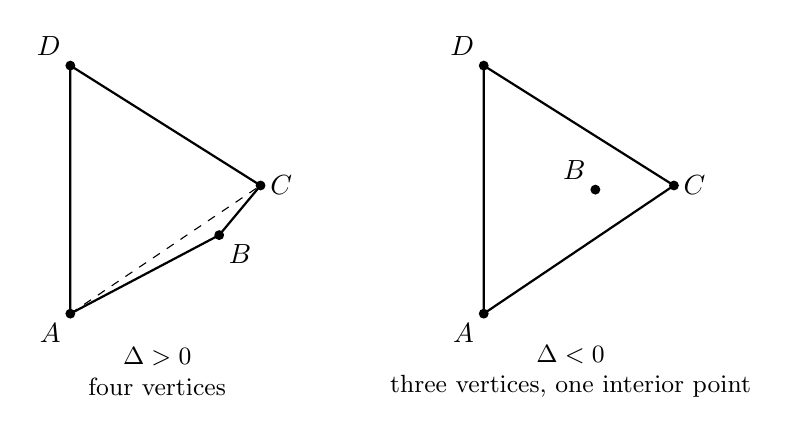
\begin{tikzpicture}[scale=1.05]
\begin{scope}
 \coordinate (A) at (0,0); \coordinate (B) at (1.8,0.95);
 \coordinate (C) at (2.3,1.55); \coordinate (D) at (0,3.0);
 \draw[thick] (A)--(B)--(C)--(D)--cycle;
 \draw[dashed] (A)--(C);
 \foreach \p/\pos in {A/below left,B/below right,C/right,D/above left}
 {\fill (\p) circle (1.7pt);\node[\pos] at (\p) {$\p$};}
 \node[align=center,font=\small] at (1.05,-0.7) {$\Delta>0$\\four vertices};
\end{scope}
\begin{scope}[xshift=5.0cm]
 \coordinate (A) at (0,0); \coordinate (B) at (1.35,1.5);
 \coordinate (C) at (2.3,1.55); \coordinate (D) at (0,3.0);
 \draw[thick] (A)--(C)--(D)--cycle;
 \foreach \p/\pos in {A/below left,B/above left,C/right,D/above left}
 {\fill (\p) circle (1.7pt);\node[\pos] at (\p) {$\p$};}
 \node[align=center,font=\small] at (1.05,-0.7) {$\Delta<0$\\three vertices, one interior point};
\end{scope}
\end{tikzpicture}
\caption{The two hull types detected by $1-fg$. Here the schematic label
$A$ denotes $A_0$. The drawing exaggerates the displacement of $B$ from
the diagonal; it is not a real-scale plot of infinitesimal coordinates.}
\label{poly:ts:fig:four}
\end{figure}

\subsection{A universal reciprocal-series construction}
The alternating example can be generalized from a periodic pattern to an
arbitrary prescribed pattern.

\begin{theorem}[Universal binary coordinate-truncation histories]\label{poly:ts:thm:universal}
Let $(\sigma_N)_{N\ge1}$ be any sequence in $\{-1,1\}$ with
$\sigma_1=1$. There are power series $f,g\in\Q[[t]]$, convergent on a
common real neighborhood of zero, such that
\begin{equation}\label{poly:ts:eq:fgconditions}
 fg=1,\qquad f=1-t+O(t^2),\qquad g=1+t+O(t^2),
\end{equation}
and, for every $N\ge1$,
\begin{equation}\label{poly:ts:eq:universal-defect}
 1-f_{\le N}g_{\le N}=\sigma_N t^{N+1}+O(t^{N+2}).
\end{equation}
The hull of the common degree-$N$ truncations of~\eqref{poly:ts:eq:fourpoints}
is therefore a quadrilateral for $\sigma_N=1$ and a triangle for
$\sigma_N=-1$. Every prescribed binary history from degree two onward
occurs in this way.
\end{theorem}
\begin{proof}
Define
\begin{equation}\label{poly:ts:eq:H-J}
 H(t)=\sum_{N\ge1}\sigma_Nt^{N-1},
 \qquad J(t)=H(t)+\frac{t^2}{4}H(t)^2.
\end{equation}
Since $H(0)=J(0)=1$, there is a unique formal square root of $J$ with
constant term $1$. Put
\begin{equation}\label{poly:ts:eq:fgconstruction}
 \begin{split}
 g(t)&=1+\frac{t^2}{2}H(t)+t\sqrt{J(t)},\\
 f(t)&=1+\frac{t^2}{2}H(t)-t\sqrt{J(t)}.
 \end{split}
\end{equation}
The coefficients are rational: the formal square-root recursion divides
by $2$, and all the coefficients of $J$ are rational. Direct multiplication
gives
\[
 fg=\left(1+\frac{t^2}{2}H\right)^2-t^2\left(H+\frac{t^2}{4}H^2\right)=1.
\]
The constant and linear terms give~\eqref{poly:ts:eq:fgconditions}, while addition
gives the particularly useful identity
\begin{equation}\label{poly:ts:eq:sumcoeff}
 f+g=2+t^2H.
\end{equation}

Write $f=\sum_{k\ge0}b_k t^k$ and $g=\sum_{k\ge0}a_k t^k$, so
$a_0=b_0=1$. Through degree $N$, the product of the truncations agrees
with the full product $1$. At degree $N+1$, the only terms of the full
product omitted by multiplying the two degree-$N$ truncations are
$a_{N+1}b_0+a_0b_{N+1}=a_{N+1}+b_{N+1}$. By~\eqref{poly:ts:eq:sumcoeff},
this sum equals $\sigma_N$. The coefficient of degree $N+1$ in the
truncated product is therefore $-\sigma_N$, proving
\eqref{poly:ts:eq:universal-defect}.

It remains to verify convergence and the hull interpretation. The series
$H$ converges absolutely for $|t|<1$. One can use a common quantitative
neighborhood, independent of the sign sequence. For complex $|t|\le1/8$,
\[
 |H(t)-1|\le\frac17,\qquad |H(t)|\le\frac87,
 \qquad |J(t)-1|\le\frac17+\frac1{196}=\frac{29}{196}<1.
\]
The binomial series for $\sqrt{1+(J-1)}$ consequently converges near this
closed disk and selects the root with constant term $1$. The two series
in~\eqref{poly:ts:eq:fgconstruction} are convergent near zero. The construction
thus works both analytically and formally, and its formal values at
$t=\omega^{-1}$ are legitimate surreal normal forms.

For every $N\ge1$, $g_{\le N}=1+t+O(t^2)$ and
$f_{\le N}=1-t+O(t^2)$. The remaining side test in
Lemma~\ref{poly:ts:lem:fourpoints} is
\[
 2g_{\le N}-2+\Delta_N=2t+O(t^2)>0.
\]
Also $g_{\le N}>0$. The first nonzero term of $\Delta_N$ is exactly
\eqref{poly:ts:eq:universal-defect}, so the lemma proves the prescribed hull type.
\end{proof}

\begin{remark}[Why the first bit is fixed]
The normalization $f=1-t+O(t^2)$ and $g=1+t+O(t^2)$ forces
$1-f_{\le1}g_{\le1}=t^2$. Thus $\sigma_1=1$ is not an overlooked
restriction: the first truncation is automatically a quadrilateral in
this normalized family. All later bits are free. This is enough to
realize every infinite binary pattern after one fixed initial stage.
\end{remark}

\begin{remark}[No contradiction with analytic nonoscillation]
For each fixed analytic family, the full identity $fg=1$ holds at every
sufficiently small real $t$. The histories above are not the signs of one
analytic function evaluated at a sequence of real arguments. Instead the
polynomials $1-f_{\le N}g_{\le N}$ themselves change with $N$. They
approach the zero function while retaining prescribed leading signs.
There is no accumulation of isolated zeros of a nonzero analytic function
at an interior point.
\end{remark}

\subsection{The final hull can be selected independently}
The full reciprocal configuration is degenerate along $A_0C$. A scale
beyond all ordinary powers removes that degeneracy without constraining
any finite truncation.

\begin{theorem}[An independent uniform transfinite endpoint]\label{poly:ts:thm:transfinite}
For the series in Theorem~\ref{poly:ts:thm:universal}, set
\[
 t=\omega^{-1},\qquad \tau=\omega^{-\omega},\qquad
 f^{(\rho)}=f-\rho\tau,\quad \rho\in\{-1,1\}.
\]
Use $f^{(\rho)}$ instead of $f$ in~\eqref{poly:ts:eq:fourpoints}. Every finite
degree-$N$ common coordinate truncation is unchanged. The full hull is a
quadrilateral if $\rho=1$ and a triangle with $B$ strictly interior if
$\rho=-1$. In both cases every three of the four full points are affinely
independent. Thus the full configuration is uniform, while its finite
coordinate-truncation history remains arbitrary.
\end{theorem}
\begin{proof}
The monomial $\tau$ is positive and smaller than $t^m$ for every ordinary
integer $m\ge0$. Its exponent position is beyond every finite degree cut,
so those cuts ignore it. The exact full determinant becomes
\[
 1-gf^{(\rho)}=1-gf+\rho g\tau=\rho g\tau.
\]
It has sign $\rho$. The remaining side test is
$2g-2+\rho g\tau$, whose leading term is $2t>0$. The other two
oriented determinants are $2g>0$ and $2>0$. Apply
Lemma~\ref{poly:ts:lem:fourpoints}. The four determinants in
\eqref{poly:ts:eq:four-dets} are all nonzero and enumerate all triples up to
orientation, proving uniformity.
\end{proof}

The theorem uses transfinite scale separation only to choose the endpoint.
The arbitrary finite-degree history itself already uses ordinary convergent
power series. For the simple alternating history, one may retain the
rational $f=(1+t)^{-1}$, $g=1+t$ of
Theorem~\ref{poly:ts:thm:alternation}. Then the full uniform example lies in
$\Q(t,\tau)^2$ coordinatewise. It is not necessary to use an arbitrary
analytic series to obtain infinitely many changes with a uniform endpoint.

\subsection{Where ordinary power-series stability returns}
\begin{proposition}[Finite determinacy for uniform ordinary series]\label{poly:ts:prop:generic-stability}
Let $V(t)$ be a configuration of $n\ge d+1$ points with coordinates in
$\R[[t]]$. Suppose every $(d+1)$-point affine determinant is nonzero.
Let $M$ be the maximum of the finite orders of these determinants.
For every $N\ge M$, the common degree-$N$ coordinate truncation has the
same signs of all these determinants, and hence the same oriented matroid
and face lattice, as the full configuration.
\end{proposition}
\begin{proof}
All coordinate entries have nonnegative order. Truncating them at degree
$N$ changes each entry by a series of order at least $N+1$. Expand a
homogeneous affine determinant by multilinearity in its columns, including
the constant homogeneous row. In every term of the difference between the
full determinant and the truncated determinant, at least one entry is a
truncation error and all remaining entries have nonnegative order.
The determinant error therefore has order at least $N+1$.

Each original nonzero determinant has order at most $M\le N$, so its
first nonzero coefficient survives unchanged. The sign pattern of the
maximal homogeneous minors determines the oriented matroid of a uniform
configuration and its supporting facets. In this uniform case one can
also recover facets directly: a $d$-point candidate facet is supporting
exactly when all determinants obtained by appending another point have
one weak orientation, which here is strict. Hence the face lattice is
unchanged.
\end{proof}

The two hypotheses explain the boundary sharply. In the rational
alternating example, a full affine determinant is identically zero, so
it has no finite leading order to protect. In the transfinite uniform
example, the previously zero determinant has order $\omega$ relative
to the monomials $\omega^{-\gamma}$; no ordinary $N$ reaches that order.
Thus ordinary uniformity plus ordinary power-series support is a genuine
stability regime, while full surreal uniformity alone is not.

\subsection{A second truncation convention that must be excluded}
Even with a fixed real base, deleting the \emph{leading} part and retaining
a tail is not covered by the lifting theorem. For example, take a square
and place a height $u(t)=\sum_{k\ge0}(-t)^k$ at one vertex, with the other
three heights zero. The unique circuit evaluates to $u$ up to a fixed
nonzero real factor. The tail starting at degree $N$ has leading sign
$(-1)^N$, so the induced diagonal alternates. This is a tail history, not
an initial-prefix history. The distinction is mathematical, not terminological.

\section{Algorithms, verification, and proof boundaries}\label{poly:ts:sec:verification}

\noindent\wtag{} Manuscript~02's finite certificate workflow and its
query-model bound \cref{poly:ts:prop:oracle} are printed in
\cref{poly:sec:computation}, and its proposed Lean development in
\cref{poly:sec:formalization}. The program is shipped as
\nolinkurl{code/02-transfinite-scales-verify.py}; its outputs are shipped
as \nolinkurl{data/02-transfinite-scales-verification.json},
\nolinkurl{data/02-transfinite-scales-hexagon_example.json} and
\nolinkurl{data/02-transfinite-scales-universal_history_example.json}, and
the captured run as \nolinkurl{data/02-transfinite-scales-verification_run.txt}.

\subsection{Recorded exact-arithmetic tests}\label{poly:ts:sec:tests}
The accompanying \nolinkurl{code/02-transfinite-scales-verify.py} uses Python's standard-library
\texttt{fractions.Fraction}. It requires no external Python package or
network access. The recorded run passed \textbf{163,914 exact assertions}.
These assertions cover the following finite cases.

\begin{table}[htbp]
\centering
\caption{Scope of the supplied finite verification.}\label{poly:ts:tab:verification}
\begin{tabular}{@{}p{0.28\textwidth}p{0.65\textwidth}@{}}
\toprule
Family & What was checked\\
\midrule
Sharp polygons & All nine sizes $4\le n\le12$: selected quotient rank,
all prefix cell sets, refinement, and all basis-slack signs after the
explicit rational specialization.\\[3pt]
Redundant-row examples & Thirty seeded arrays of thirteen rational rows,
including affine components and redundant coefficient directions:
original and compressed prefix signs, cells, and real specialization.\\[3pt]
Universal histories & All $2^7=128$ sign histories of length eight with
first bit positive; twelve seeded histories of length thirty-two; one
additional length-twelve example. Reciprocal jets, leading defect
coefficients, and side-orientation signs were checked exactly.\\[3pt]
Rational alternation & The full polynomial identity
\eqref{poly:ts:eq:alternating-defect} for each $1\le N\le64$.\\
\bottomrule
\end{tabular}
\end{table}

The count measures individual assertions, not independent theorems or
statistical confidence. In particular, none of these tests proves the
quantification over all real functionals, arbitrary infinite sign
sequences, transfinite supports, or all dimensions. Those claims rest on
the written proofs. The deterministic seeds are $20260930$ for the
compression tests and $31415926$ for the longer history samples.
The machine-readable output is \nolinkurl{data/02-transfinite-scales-verification.json}; the
hexagon and a prescribed-history coefficient example have separate JSON
files.

The program uses a coefficient recursion equivalent to the closed
construction~\eqref{poly:ts:eq:fgconstruction}; Appendix~\ref{poly:ts:app:recurrence}
derives it. This supplies a second algebraic view of the main negative
example. There is no numerical approximation to $\omega$ in the program.

\subsection{A proof dependency audit}\label{poly:ts:sec:audit}
The delicate assumptions are summarized in Table~\ref{poly:ts:tab:audit}.
These are boundaries of the results, not optional technicalities.

\begin{longtable}{@{}p{0.28\textwidth}p{0.65\textwidth}@{}}
\caption{Hypotheses whose omission would change or invalidate the claim.}\label{poly:ts:tab:audit}\\
\toprule
Result & Essential boundary\\
\midrule
\endfirsthead
\toprule
Result & Essential boundary\\
\midrule
\endhead
\bottomrule
\endfoot
Lifting compression & The base coordinates and comparison coefficients
are real and fixed. Moving coordinates lead to nonlinear determinant
expressions and are not covered.\\[4pt]
History preservation & Cuts retain common initial normal-form segments.
Independent coordinate cuts, sign-sequence cuts, and tail deletion are
different operations.\\[4pt]
Rank minimality & All real affine-dependence signs, including zero, are
preserved. A finite circuit list or one final subdivision may require less
information.\\[4pt]
Real specialization & The explicit bound protects a finite family of
functionals. It does not embed the entire higher-rank ordered comparison
space into $\R$.\\[4pt]
Refinement chains & Marked cell-label inclusion is used. Geometric
containment alone can conceal whether an interior point is on the
lower hull.\\[4pt]
Universal histories & The degree-one bit is forced positive by the
normalization. The freely prescribed history starts at degree two.
There are four generators, not necessarily four extreme vertices.\\[4pt]
Uniform endpoint & An added monomial beyond all ordinary powers chooses
the endpoint. This is not an ordinary analytic correction with a finite
Taylor order.\\[4pt]
Ordinary stability & All relevant maximal determinants are nonzero and
have finite orders, and coordinates have nonnegative orders.\\[4pt]
Standard-part geometry & Coordinates are finite. The polar identity
uses only finite polar points; a face image need not be a face.\\[4pt]
Puiseux realization & Only finitely many polynomial observations and
incidences are preserved. Curve selection and convergent algebraic
Puiseux expansions are classical imported theorems.\\[4pt]
Computations & Exact finite arithmetic tests selected examples. No Lean
build, general surreal algorithm, or independent proof certification
was performed.\\
\end{longtable}

\section{Further research questions}\label{poly:ts:sec:future}

The following are proposed research directions arising from this article.
They are not assertions that each topic is absent from the literature, nor
are they labeled as longstanding published open problems. The first three
would most directly deepen the results proved here.

\subsection{Which histories admit rational-function coordinates?}
The universal construction permits arbitrary convergent reciprocal power
series, while rational functions already give a periodic alternating
history. Characterize the binary histories realizable by four points of
the form~\eqref{poly:ts:eq:fourpoints} with $f,g\in\Q(t)$ and $fg=1$.
In the normalized reciprocal setting, the degree-$N+1$ coefficient of
the degree-$N$ truncation defect equals that of $f+g$. When nonzero it
determines the history bit; a zero requires looking at higher degrees.
For rational functions, the coefficients of $f+g$ satisfy a linear
recurrence after finitely many indices. The problem therefore links geometric truncation histories
to sign patterns of rational generating functions, with the additional
constraint that the generating function is a reciprocal sum. A useful
first target is a classification of eventually periodic histories and a
precise description of the extra reciprocal constraint.

\subsection{Stability in the presence of exact incidences}
Proposition~\ref{poly:ts:prop:generic-stability} treats configurations whose
maximal determinants are all nonzero. The universal examples exploit a
zero full determinant whose truncations have arbitrary leading signs.
Find a necessary and sufficient condition, in a specified algebraic or
analytic representation class, for the \emph{zero} determinant relations
to have eventually stable truncation signs. A condition merely on the
final oriented matroid cannot suffice. Possible additional data include
how an incidence ideal interacts with the coordinate truncation maps,
and bounds on cancellation in products of truncated coordinates.

\subsection{Effective controlled specialization}
Theorem~\ref{poly:ts:thm:puiseux} is qualitative. Given rational polynomial
incidence data, a compatible algebraic standard-part configuration, and
a realizable sign pattern, obtain explicit bounds on a Puiseux arc's ramification,
algebraic degree, and coefficient height. An especially useful version
would preserve selected vanishing orders or a finite sequence of near-face
optimality bands in addition to the final face lattice. Such a theorem
must distinguish geometric sign complexity from the bit complexity of
an exact coefficient representation.
\wtag{} Manuscript~05's question~1 (\cref{poly:sec:questions}) asks the same
for determinant signs; \cref{poly:mv:thm:compression} of
\cref{poly:part:mv} gives an effective specialization for finite-support
Hahn certificates.
[\wtag{} \Cref{poly:part:cd} gives a lower-bound family for rational arcs
(\cref{poly:cd:thm:main}); no upper bound of the kind asked is proved.]

\subsection{Minimal geometric certificates versus full comparison rank}
The rank $p$ classifies how many coefficient layers are needed to preserve
all real affine comparisons, whereas the strict history length $r$ can
be smaller. Determine an efficient canonical quotient of the comparison
data that preserves just the marked subdivision history. How small can a
slack or circuit certificate be compared with the all-basis list? What is
the complexity of extracting it for a fixed dimension, and which
families admit polynomial-size certificates without enumerating every
candidate basis? A single final subdivision cannot determine $p$; any
proposed invariant must respect that information loss.
\wtag{} Manuscript~05's question~4 (\cref{poly:sec:questions}) asks the same
for face lattices, lower subdivisions and toric initial ideals together.

\subsection{A replacement for the false residue map on faces}\label{poly:ts:q:residue}
The image of a face under standard part need not be a face. Develop a
polyhedral object whose cells retain the fibers, infinitesimal widths,
and near-optimality data discarded by ordinary residue. The identity in
Proposition~\ref{poly:ts:prop:band} suggests indexing such data by objective
functionals and admissible infinitesimal error levels. The challenge is
to obtain an intrinsic finite description when one exists, and to state
precisely when transfinite scale labels are unavoidable.
\wtag{} Related: the questions of \cref{poly:part:mv} on face specialization
and oriented scale data and on joint residue data ask for structures of the
same kind; \cref{poly:ts:prop:band} is the single-objective case.

\subsection{Beyond linear comparisons: realizability constraints}
One can apply linear compression to a finite list of determinant values
regarded as unrelated surreal scalars. That does \emph{not} show that
the compressed values are minors of an actual point configuration:
Pl\"ucker relations and other polynomial dependencies may fail.
Determine which rank-compression operations preserve realizability of
valued or oriented matroid data. A useful theorem would identify a
nontrivial class in which support compression can be lifted back to
coordinate matrices without changing prescribed signs and selected
valuation comparisons.
\wtag{} Manuscript~05's question~2 (\cref{poly:sec:questions}) asks this for
two nonreal lifting coordinates over a fixed real base.

\subsection{Infinite locally finite configurations}
The proof of Theorem~\ref{poly:ts:thm:compression} depends on finite dimension of
the coefficient quotient, not on a bound for support length. For infinite
configurations the affine relation space is generally infinite dimensional.
Which local finiteness, support, or uniform-rank assumptions imply local
stabilization of coherent subdivisions? A satisfactory formulation should
specify whether stabilization is pointwise on finite subconfigurations,
uniform on bounded regions, or global. The four-point examples show that
coordinatewise convergence alone is too weak even before infinitude is
introduced.

\subsection{Formalization and representation-aware computation}
Carry out the layered Lean program in \cref{poly:ts:sec:leanplan} and
attach a checked theorem ledger. In parallel, classify effective
representations for which the next rank-increasing coefficient can be
found or its absence certified. Finite support with a known bound,
rational functions, algebraic series, and general coefficient oracles
have materially different capabilities. Proposition~\ref{poly:ts:prop:oracle}
shows that an implementation cannot hide those differences behind a
single unrestricted ``surreal input'' interface.
\wtag{} Manuscript~02's layered Lean program is printed in
\cref{poly:sec:formalization}; manuscript~05's question~5
(\cref{poly:sec:questions}) asks for such representations from the side of
\cref{poly:prop:undecidable}.


\section{Conclusion}
Finite surreal geometry has two distinct levels. At the level of a single
finite incidence pattern, real-closed-field transfer gives an ordinary
real algebraic model. At the level of a fixed real base with surreal
lifting heights, finite-dimensional linear algebra still controls all
normal-form prefix histories: at most $n-d-1$ effective comparison layers
are needed, and that bound is sharp.

Neither fact controls arbitrary coordinate truncation. Four bounded
planar generators can encode any binary triangle/quadrilateral history
from degree two onward, and a transfinite monomial can independently
choose a uniform final endpoint. Thus the relevant additional structure
of surreal polytopes is not a previously impossible finite face lattice.
It is the organization of incidence data across scales, together with
the precise operations used to expose or forget those scales.

\section{An exact recursion for the universal construction}\label{poly:ts:app:recurrence}
\noindent\wtag{} Appendix~A of manuscript~02.

The closed formula~\eqref{poly:ts:eq:fgconstruction} is convenient for proving
convergence. For exact finite calculations, the following recursion avoids
formal square-root software. Write
\[
 g=\sum_{k\ge0}a_k t^k,\qquad f=\sum_{k\ge0}b_k t^k,
 \qquad a_0=b_0=1,\ a_1=1,\ b_1=-1.
\]
For $n\ge2$, assume the previous coefficients have been chosen and set
\begin{equation}\label{poly:ts:eq:recursion}
 \begin{split}
 c_n&=-\sum_{k=1}^{n-1}a_k b_{n-k},\\
 M_n&=\sum_{k=2}^{n-1}a_k b_{n+1-k},\\
 a_n&=\frac{\sigma_n+c_n+M_n}{2},\qquad b_n=c_n-a_n.
 \end{split}
\end{equation}
The equality $a_n+b_n=c_n$ forces the degree-$n$ coefficient of $fg$
to vanish. The coefficient of degree $n+1$ in the product of the two
degree-$n$ truncations is
\[
 a_1b_n+a_nb_1+M_n=b_n-a_n+M_n=c_n-2a_n+M_n=-\sigma_n.
\]
Thus the leading truncation defect is $\sigma_n$. At the next step the
condition of being reciprocal forces $a_{n+1}+b_{n+1}=\sigma_n$.
Together with $a_2+b_2=1=\sigma_1$, this reproduces
$f+g=2+t^2H$.

Conversely, the identities $fg=1$, $f+g=2+t^2H$, and the linear terms
$g=1+t+O(t^2)$, $f=1-t+O(t^2)$ select exactly the branch in
\eqref{poly:ts:eq:fgconstruction}. Hence the recursion computes that same pair.
Every requested sign prefix determines the corresponding finite jets;
an arbitrary continuation of the signs completes them to the convergent
series of Theorem~\ref{poly:ts:thm:universal}.

For example, $\sigma_2=1$ gives $a_2=1$, $b_2=0$, whereas
$\sigma_2=-1$ gives $a_2=0$, $b_2=1$. These yield, respectively,
positive and negative leading degree-three defects. Later sign choices
are independent and are obtained by the same rational recursion.

\section{Reproducibility and source inventory}\label{poly:ts:app:repro}
\noindent\wtag{} Appendix~B of manuscript~02; in this report its files are
shipped under prefixed names. \nolinkurl{code/verify.py} is
\nolinkurl{code/02-transfinite-scales-verify.py}; the three generated JSON
files are \nolinkurl{data/02-transfinite-scales-verification.json},
\nolinkurl{data/02-transfinite-scales-hexagon_example.json} and
\nolinkurl{data/02-transfinite-scales-universal_history_example.json}; the
\nolinkurl{Makefile} is \nolinkurl{code/02-transfinite-scales-Makefile};
the source and proof-audit notes are
\nolinkurl{02-transfinite-scales-sources.md} and
\nolinkurl{02-transfinite-scales-proof_audit.md}; the build record
\nolinkurl{notes/validation.json} is
\nolinkurl{data/02-transfinite-scales-validation.json} and describes the
delivered PDF. The manuscript's \nolinkurl{article.tex}, PDF and README are
not shipped: this report replaces them. The commands below name the
delivered layout; run them on a copy (the report's README gives the recipe).

The archive contains \texttt{article.tex}, its compiled PDF,
\texttt{code/verify.py}, the three generated JSON data files, a
\texttt{Makefile}, a README, and separate source and proof-audit notes.
From the archive directory, run
\begin{quote}\ttfamily
python3 code/verify.py\\
pdflatex -interaction=nonstopmode -halt-on-error article.tex\\
pdflatex -interaction=nonstopmode -halt-on-error article.tex
\end{quote}
The verification script resolves its output paths relative to itself.
The PDF build uses ordinary TeX packages and no shell escape, external
bibliography processor, or network call. The \texttt{Makefile} performs
an extra TeX pass for stable cross-references. No font files are distributed.

The repository geometry file inspected at the pinned commit has blob
identifier
\begin{center}\small\texttt{450fd4bbfc017e0da24c28e538af1cc02037ad5a}.\end{center}
The code-search index observed during the source check pointed to parent
commit
\begin{center}\small\texttt{5e0f4e05046bacda3c6ba2643f19b91aa632436b}.\end{center}
The actual geometry source was then read at the full pinned commit. This distinction is
recorded to avoid presenting search-index freshness as a repository-wide
proof audit. No original repository files were modified.


\part{Affine residues and mixed-volume scales}\label{poly:part:mv}

\paragraph{Source and scope.}\wtag{} This Part prints, whole, manuscript~06 of
batch~58: \emph{Surreal Polytopes: Affine Residues, Mixed-Volume Scales, and
Simultaneous Segment Models}, headed ``ProveIt research program'', author line
``Research article prepared for Vladimir Reshetnikov'', dated 30~September 2026
(archive \pathcode{Surreal_Polytopes_Research_Package.zip}, main file
\pathcode{Surreal_Polytopes/article.tex}; delivered PDF of 27 pages, not
shipped). It was written against ProveIt commit \pathcode{6996fee43}. Its
program, recorded run, build file and provenance note are shipped as
\pathcode{code/06-affine-residues-verify.py},
\pathcode{data/06-affine-residues-verification.json},
\pathcode{code/06-affine-residues-Makefile} and
\pathcode{06-affine-residues-PROVENANCE.md}. Its README and checksum list
\texttt{SHA256SUMS} are not shipped; they survive in the delivery archive of
arrival commit \pathcode{b2b626d85}. Every
section, result, proof, example, remark, figure, table and research question of
the manuscript is printed here, in the manuscript's order, with three
structural changes: its appendix is printed as the ordinary
\cref{poly:mv:app:audit}; its subsection ``A modular Lean development'' is
printed in the formalization chapter (\cref{poly:mv:sec:formalization}); and
its bibliography is printed as the list ``References of Part~III''. This Part
is its own spine (the residue/volume spine of \cref{poly:sec:guide}); it shares
no theorem with the other Parts beyond two foundations, both marked where they
occur: the standard part of a finite hull (\cref{poly:mv:lem:hull-reduction},
proved in Part~I as \cref{poly:prop:stconv}) and finite real-closed-field
transfer (\cref{poly:mv:prop:faces}, Part~I's \cref{poly:thm:general}). The
Part keeps its own definitions and hypotheses, fixed in
\cref{poly:mv:sec:intro,poly:mv:sec:foundations}. In this Part ``the article''
and ``the package'' mean manuscript~06 and its delivery. Where manuscript~06
says ``the report'', it means itself or, in \cref{poly:mv:sec:verification},
its recorded run. It never means this merged report.

\emph{Generality.} Although manuscript~06 and this report have ``surreal'' in
their titles, every theorem of this Part is proved for an \emph{arbitrary}
set-sized real closed ordered field $K\supseteq\R$ with its natural convex
valuation (the standing hypothesis stated at the end of the first subsection
below). The surreal field enters only as the source of examples: finitely many
surreal coordinates lie in such a $K$ (\cref{poly:mv:sec:foundations}), and
$\omega^{-1}$, $\omega^{-\omega}$ occur only in examples and in the audit. The
word ``surreal'' in the titles is therefore not a hypothesis of any result
here.

\paragraph{Notation in this Part.}\wtag{} The following symbols mean something
different elsewhere in the report (\cref{poly:sec:notation}); the Part-local
meaning is the one in force here.
\begin{itemize}
\item $\OO$ is the ring of elements of $K$ bounded by real constants and $\mm$ its
  maximal ideal: the same ring as $\cO_K$ (Parts~I--II) and $\mathcal O_K$
  (Part~IV). $\st:\OO\to\R$ is the standard part, as everywhere in the report.
\item $v:K\to\Gamma\cup\{\infty\}$, $\Gamma=K^\times/\OO^\times$, is ordered so
  that \emph{larger values mean smaller elements}: $v(x)\ge v(y)$ iff
  $x/y\in\OO$, and $v(x)>0$ iff $x\in\mm\setminus\{0\}$. The value group need
  not embed in $\R$. (Part~I's leading exponent measures growth, in the
  opposite direction; Part~V writes $\nu$ and $\vv$.)
\item The \emph{affine residue} $\Res(P)$ (\cref{poly:mv:def:affine-residue}) is a
  renormalised, dimension-preserving real polytope, the image of $P$ in
  $(p_0+L(P))/\mm L(P)$. \emph{It is not the standard part} $\st P$: the thin
  triangle of \cref{poly:mv:sec:examples} has $\st P$ a segment but $\Res(P)$ a
  triangle. Where this Part says ``residue field'', ``reduction'' or ``volume
  residue'' (\cref{poly:mv:prop:volume-reduction}), it means the standard part.
  The report reserves ``affine residue'' for $\Res$.
\item $L(P)=\spanplain_{\OO}(P-P)$ is the \emph{scale lattice}, a free
  $\OO$-module, not a discrete subgroup; it is unrelated to Part~I's $L_h$ and
  $L_A$ and to Part~IV's lattice-point count $L_P(n)$.
\item $\MV(P_1,\ldots,P_d)$ (printed $\operatorname{V}$) is mixed volume, not
  Part~I's dependence space $V$ or Part~V's coarse ring. $\Vol_d$ is determinant
  (triangulation) volume; Part~IV writes $\vol_d$ for Euclidean volume of real
  polytopes.
\item $m$ is the number of bodies (not Part~I's comparison rank, not Part~V's
  $m$ with $n=2^m$); $r$, $r_i$ are affine dimensions (not Part~II's history
  length or Part~I's shadow rank $r_0$); $q(B)=v\det W_B$ in
  \cref{poly:mv:lem:valued-exchange} (not $q=n-d-1$); $H$ is the grid bound
  $\binom{m-1}{d-1}$ in \cref{poly:mv:thm:segments} and a finitely generated
  group in \cref{poly:mv:lem:grading}; $S_i$ are inner segments and $T_i$ probe
  segments (not Part~IV's trace $S$ and implanted polytope $T$, not Part~V's
  slack matrix and triangle); $\rho_g$ is the sign threshold of a specialized
  Laurent polynomial in \cref{poly:mv:sec:compression} (Part~I's threshold is
  $\eta$); $s$ is the real specialization parameter and $t^\gamma$ a formal
  Hahn monomial there (Part~II's $t$ is a power-series variable evaluated at $t=\omega^{-1}$).
\item $\tau_I$, $\tau(\alpha)$ and ``the profile $\tau$'' are the pure and full
  mixed-volume valuation profiles; they are \emph{not} powers of the surreal
  $\tau=\omega^{-\omega}$ of the other Parts. Manuscript~06 writes $\eta$
  for $\omega^{-\omega}$ (in its examples, in \cref{poly:mv:sec:compression}
  and in its audit), and this Part keeps that letter so that $\tau$ means only
  a profile here; $\eps=\omega^{-1}$ as in the source. Part~I's $\eta$ is a
  different object (a sign threshold).
\item Macro change only: manuscript~06's \verb|\Span| (plain span over the ring
  or field in context) is typeset with the report's \verb|\spanplain|; the
  printed output is unchanged.
\end{itemize}

\paragraph{Abstract of manuscript 06.}
Finite polytopes over the surreal numbers have no new finite face-lattice
possibilities merely because the coordinates are surreal. Their genuinely
non-Archimedean information lies instead in relative scales, cancellation,
and degeneration. We develop an algebraic treatment of that information
inside set-sized real closed subfields of the surreal field.

The principal result is a simultaneous inner-segment theorem: for every
finite family of polytopes, a segment can be chosen inside each member so
that all mixed-volume valuations involving distinct members are preserved
at once. Consequently the pure mixed-volume valuation configurations are
exactly the determinant-valuation configurations realizable over the given
ordered field. A finite rational grid suffices for the segment choices.
Applying the theorem to labelled copies of the bodies produces a
representable valuated-matroid model of the entire mixed-volume profile,
and proves its exchange-convexity for arbitrary ordered value groups.

The underlying invariant is the translation-invariant module
$L(P)=\spanplain_{\OO}(P-P)$, where $\OO$ is the ring of finite elements.
A maximum vertex simplex gives an explicit basis of this module and a
full-dimensional real affine residue, even when ordinary standard part
collapses the original polytope. Mixed-volume valuations depend only on
these modules and admit certificates using at most $d^d$ determinants per
coefficient after basis selection. Conversely, a full-dimensional module
is determined by mixed-volume probes, with a $d+1$-measurement comparison
test relative to a reference polytope.

Detailed proofs, higher-rank examples, finite-support specialization,
exact computational audits, and a research agenda are provided. The
classical ingredients and the unverified priority of the combined results
are identified explicitly; no solution of the full real mixed-volume
configuration problem or new Lean formalization is claimed.

\paragraph{Scope (title page of manuscript 06).}
Finite vertex sets; fixed finite dimension; the natural
convex valuation; exact algebraic volume. No proper-class integration,
Archimedean valuation hypothesis, or sequential compactness argument is used.


\section{Research target, principal results, and status}
\label{poly:mv:sec:intro}

\subsection{Why the finite combinatorics is not the whole question}
Replacing real coordinates by surreal coordinates does not, by itself,
create new finite combinatorial types of polytopes. The incidence data of
a fixed finite vertex configuration can be encoded in the first-order
theory of real closed fields. That observation is useful, but it does not
explain a triangle of height $\omega^{-1}$, a determinant whose first
nonzero term occurs at $\omega^{-\omega}$, or the mixed volume of two
bodies thin in different directions.

The appropriate questions are more precise. Can one normalize a finite
surreal polytope without destroying its affine dimension? Which finite
algebraic data determine the scale of a mixed volume? Can all the scales
of a family be realized simultaneously by much simpler objects? Can the
resulting scale information be recovered from measurements? The article
answers these questions under explicit hypotheses.

Throughout the main results, $K$ is a set-sized real closed ordered field
containing $\R$, $\OO$ is its ring of elements bounded by real constants,
and $v:K\to\Gamma\cup\{\infty\}$ is the corresponding valuation. The
surreal application takes $K$ inside $\No$. Our convention is that larger
valuations mean smaller quantities. The value group $\Gamma$ need not
embed in $\R$.

\subsection{The principal theorem in a compact form}
For nonempty finite polytopes $P_1,\ldots,P_m\subset K^d$, put
\[
 \tau_I=v\bigl(\MV(P_{i_1},\ldots,P_{i_d})\bigr),
 \qquad I=\{i_1<\cdots<i_d\}\subseteq[m].
\]
We call this the \emph{pure} profile: every body occurs at most once in an
entry. The mixed-volume convention is $\MV(P,\ldots,P)=\Vol_d(P)$.

\begin{theorem}[Simultaneous inner-segment model, preview]
\label{poly:mv:thm:preview}
For $m\ge d\ge1$, there are segments $S_i\subseteq P_i$, possibly reduced
to points, such that
\[
 v\bigl(\MV(S_{i_1},\ldots,S_{i_d})\bigr)=\tau_I
 \quad\text{for every }I\in\binom{[m]}d.
\]
The segments may be chosen with endpoints that are rational convex
combinations of vertices of their respective polytopes.
\end{theorem}

The proof in Section~\ref{poly:mv:sec:segments} does more than choose a generic
point informally. After selecting at most $d$ vertex directions in each
body, it gives a finite rational grid containing a successful simultaneous
choice. If $S_i=[p_i,p_i+w_i]$, the segment formula becomes
\[
 \tau_I=v\det(w_{i_1},\ldots,w_{i_d}),
\]
with $v(0)=\infty$. Thus every pure profile has a single matrix realization,
not merely a different determinant witness for each entry.

Repetitions matter. Replacing a full-dimensional body by one segment cannot
preserve its ordinary volume in dimension greater than one. For the
\emph{full} profile, which includes repetitions, we use either parallelotopes
with at most $d$ generators or $d$ separately labelled segment copies of
each body. The clone construction retains all repeated-body valuations and
implies a higher-rank discrete exchange inequality
(Theorem~\ref{poly:mv:thm:mconvex}).

\subsection{What the other theorems add}
For a polytope $P$, define its \emph{scale lattice}
\[
 L(P)=\spanplain_{\OO}(P-P).
\]
The word lattice here means a finitely generated free $\OO$-module in a
finite-dimensional $K$-space; it does not mean a discrete subgroup in the
Euclidean sense. The following results describe the geometry behind the
segment theorem.

\begin{center}
\begin{tabular}{@{}p{0.24\textwidth}p{0.69\textwidth}@{}}
\toprule
Result & Content and location\\
\midrule
Affine normalization & A maximum vertex simplex generates $L(P)$;
normalization lies between a standard simplex and a cube. The residue
preserves affine dimension (Section~\ref{poly:mv:sec:residue}).\\[0.5em]
Mixed determinant formula & Every mixed-volume valuation is the minimum
valuation of one-direction-per-body determinants; selected bases need at
most $d^d$ such determinants (Section~\ref{poly:mv:sec:determinants}).\\[0.5em]
Simultaneous simplification & Inner segments preserve all pure entries;
parallelotopes preserve the full profile
(Sections~\ref{poly:mv:sec:determinants}--\ref{poly:mv:sec:segments}).\\[0.5em]
Discrete convexity & A clone realization gives the exchange axiom over
any ordered value group, without a real-valued grading
(Section~\ref{poly:mv:sec:profiles}).\\[0.5em]
Reconstruction & All segment probes characterize $L(P)$; a reference
basis gives a finite $d+1$-measurement test
(Section~\ref{poly:mv:sec:probes}).\\[0.5em]
Finite certification & Finite-support higher-rank input admits a
one-parameter model preserving specified finite certificates, but not the
whole higher-rank order (Section~\ref{poly:mv:sec:compression}).\\
\bottomrule
\end{tabular}
\end{center}

\subsection{Repository provenance and dependence}
The inspected ProveIt snapshot is commit
\pathcode{6996fee43cc97b6c16351def7507d59a95bf62f0}, retrieved on
30 September 2026. The relevant development is
\pathcode{Algebra/SurrealNumbers}; its README records the constructed
surreal ordered field, real-closedness, and a statement-level formalization
ledger \cite{mv:RepoSurreal}. The report also draws a methodological
connection to the finite support certificates in
\emph{Reversion Beyond Archimedean Valuations} under
\pathcode{Analysis/Transseries} \cite{mv:RepoReversion}.

The inspection was targeted, not a complete audit of the repository.
Search results were used for navigation; the principal source files were
read at the immutable commit above. In particular, this article does not
assume the correctness of every research claim in the repository. Its
mathematical prerequisites are the classical real-closedness of the surreal
field, elementary valuation algebra, and finite real polytope theory.
The proofs below are independent of the repository's unrefereed advanced
analytic claims.

\noindent[\wtag{} Re-verified at the write phase. The Transseries report
cited here is at
\pathcode{Analysis/Transseries/docs/series-and-transseries/Reversion_Beyond_Archimedean_Valuations/},
with title and subtitle exactly as in the bibliography entry
\cite{mv:RepoReversion}; its finite positive-grading result, credited below
as the antecedent of \cref{poly:mv:lem:grading}, is the theorem ``Finite
supports admit a positive rational grading'' there. The SurrealNumbers
README still describes the constructed ordered field, its real-closedness
and the formalization ledger. Nothing in this Part is formalized in Lean
(see \cref{poly:mv:sec:formalization}).]

\subsection{Literature boundary and novelty}
Ordered-field polyhedral geometry is established mathematics; a modern
formal treatment of face lattices over ordered fields is given by
Allamigeon, Katz, and Strub \cite{mv:AKS}. Classical mixed-volume theory,
including its determinant special case, is treated by Schneider
\cite{mv:Schneider}. Averkov, von Dichter, Richard, and Soprunov connect mixed
volumes of zonoids to absolute Grassmannian coordinates and explicitly
propose investigating a connection with tropical Grassmannians in their
November 2024 version \cite{mv:ADRS}. Our simultaneous segment theorem gives
a concrete valued-field connection for \emph{all finite polytopes}, with
a precise realization field and no closure convention hidden in the claim.

The broader link between volume polynomials, Lorentzian polynomials, and
$M$-convex tropicalizations is already part of the theory of Br\"and\'en
and Huh \cite{mv:BH}. Lattices, norms, buildings, and realizable valuated
matroids also have an extensive theory; see, for example, Battistella,
K\"uhn, Kuhrs, Ulirsch, and Vargas \cite{mv:BKKUV}. We do not claim to have
invented these connections. The contribution developed here is the
explicit package of simultaneous inner models, dimension-only determinant
certificates, affine residues, reconstruction, and arbitrary-value-group
proofs adapted to finite surreal geometry.

\begin{remark}[Status of the claims]
Every numbered theorem presented as a result is proved below, either
from identified classical facts or by an explicit algebraic argument.
Their correctness and the extent of their novelty have not been
independently refereed, and an exhaustive priority search has not been
completed. The computational supplement checks finite instances; it is not
a Lean proof. No solution of the complete real mixed-volume configuration
problem is claimed. These qualifications concern verification and priority,
not a missing step being concealed in the stated theorems.
\end{remark}

\section{Set-sized foundations and finite geometry}
\label{poly:mv:sec:foundations}

\subsection{Working inside the surreal field without a class-sized domain}
The surreal numbers form a real closed ordered class field; standard
references discuss this field and its universality properties
\cite{mv:Ehrlich}. For finitely many coordinate values, start with the
set-sized field generated by those values and $\R$, then take its real
closure inside $\No$. This yields a suitable set-sized $K$ containing all
input. The elementary algebraic constructions used here remain in such a
field.

Consequently a polytope in the article is the ordinary set
\[
 P=\conv_K\{p_1,\ldots,p_n\}
 =\left\{\sum_{i=1}^n\lambda_i p_i:
       \lambda_i\in K_{\ge0},\ \sum_i\lambda_i=1\right\}\subset K^d.
\]
This is not an assertion that the collection of \emph{all} surreal points
in the corresponding class convex hull is a set. Finite face data and
volumes are compatible with enlarging $K$: their definitions use finite
linear algebra and first-order formulas over the coefficient field.

\subsection{Finite elements, residue, and order of magnitude}
Define
\begin{align*}
 \OO&=\{x\in K:|x|\le C\text{ for some }C\in\R_{>0}\},\\
 \mm&=\{x\in K:|x|<c\text{ for every }c\in\R_{>0}\}.
\end{align*}
The ring $\OO$ is convex in $K$. For $x\ne0$, either $x$ is finite or
$1/x$ is finite, so it is a valuation ring. Its nonunits are precisely
$\mm$: a finite nonzero $x$ is a unit exactly when $|x|$ is bounded below
by a positive real constant.

\begin{lemma}[Standard part]
\label{poly:mv:lem:standard}
For each $x\in\OO$ there is a unique $r\in\R$ such that $x-r\in\mm$.
The resulting map $\st:\OO\to\R$ is an order-preserving surjective ring
homomorphism with kernel $\mm$.
\end{lemma}
\begin{proof}
The real set $\{a\in\R:a\le x\}$ is nonempty and bounded above. Let $r$
be its supremum. For every positive real $c$, the definition of supremum
gives $r-c<x<r+c$, allowing harmless weak inequalities first and then
replacing $c$ by $c/2$. Thus $x-r$ is infinitesimal. A nonzero real number
cannot be infinitesimal, proving uniqueness.

Finite sums of infinitesimals are infinitesimal, and the product of a
finite element with an infinitesimal is infinitesimal. Expanding
$(r+\epsilon)(s+\delta)$ proves preservation of multiplication; addition
is immediate. Constants give surjectivity, the kernel description follows
from uniqueness, and positivity follows from convexity.
\end{proof}

Write $\Gamma=K^\times/\OO^\times$ additively and $v(x)$ for the class of
$x\ne0$. Order it so that
\[
 v(x)\ge v(y)\quad\Longleftrightarrow\quad x/y\in\OO.
\]
Set $v(0)=\infty$, with $\gamma+\infty=\infty$. Positive real constants
have value zero. A nonzero element belongs to $\mm$ exactly when its value
is positive.

\begin{lemma}[Finite positive sums and bounded comparison]
\label{poly:mv:lem:positive}
If $a_1,\ldots,a_N\in K_{\ge0}$, then
\[
 v\left(\sum_{i=1}^N a_i\right)=\min_i v(a_i).
\]
If $0<c\le C$ are real and $0\le a,b\in K$ satisfy $cb\le a\le Cb$,
then $v(a)=v(b)$, including the case $a=b=0$.
\end{lemma}
\begin{proof}
When some $a_i$ is nonzero, choose a largest member $M$. The inequalities
$M\le\sum_i a_i\le NM$ show that the quotient of the sum by $M$ is a
unit of $\OO$. The same unit argument proves the second assertion.
The all-zero case is immediate.
\end{proof}

No assertion about infinite sums is involved. The absence of cancellation
for a finite positive sum will replace all appeals to a real-valued
valuation or an Archimedean growth parameter.

\subsection{The precise finite transfer principle}
Real closed fields satisfy quantifier elimination and have a complete
first-order theory in the ordered-field language; semialgebraic geometry
provides the usual framework \cite{mv:Coste}. In particular, $\R\subset K$
is an elementary extension. Only \emph{finite-dimensional, finitely
presented} instances are transferred here.

\begin{proposition}[No new finite face types]
\label{poly:mv:prop:faces}
Every finite polytope over $K$ has the face lattice of a polytope whose
coordinates are real algebraic numbers. Any prescribed finite collection
of rational-polynomial equalities, inequalities, and sign tests on the
vertex coordinates can be preserved simultaneously when it is included
in the realization formula.
\end{proposition}
\begin{proof}
Fix the number $n$ of labelled input points and their affine dimension.
For a nonempty subset $S\subseteq[n]$, the assertion that exactly the
labels in $S$ lie on a supporting face is expressed by
\[
 \exists a\in K^d\ \exists c\in K:
 \quad a\cdot p_i=c\ (i\in S),\qquad
       a\cdot p_i<c\ (i\notin S).
\]
The full polytope corresponds to $S=[n]$; the empty face is added
separately. Form the conjunction of this assertion or its negation for
each of the finitely many subsets $S$. Include a rank formula for the
affine dimension and the requested additional tests. Existentially
quantify the vertex coordinates. The resulting sentence has rational
coefficients and holds in $K$, hence in the real algebraic field, which
is also real closed. Its realization has exactly the same labelled face
sets and therefore the same inclusion lattice.
\end{proof}

This does not preserve the natural valuation, infinitesimal relations to
\emph{every} real constant, or a whole infinite type. Nor does it assert a
rational realization. The face-lattice result is the classical boundary
condition for the rest of the article, rather than its proposed novel
contribution.

\noindent[\wtag{} This is the finite real-closed-field transfer that Part~I
states and proves for finite configurations as \cref{poly:thm:general}
(manuscripts 05 and 02). Manuscript~06's statement and proof are kept as
printed because they are phrased for face lattices together with prescribed
sign tests. The same principle appears again as Part~IV's
\cref{poly:ehr:prop:transfer} and, strengthened to oriented matroids and
extension complexity, as Part~V's \cref{poly:ic:thm:conservativity}. The
limitations in the preceding paragraph apply to every one of these
statements.]

\section{Algebraic volume and reduction to the residue field}
\label{poly:mv:sec:volume}

\subsection{Determinant volume, not surreal measure theory}
For an affine $d$-simplex set
\[
 \Vol_d\conv(p_0,\ldots,p_d)
   =\frac1{d!}\left|\det(p_1-p_0,\ldots,p_d-p_0)\right|.
\]
A full-dimensional finite polytope admits a finite triangulation; summing
these simplex volumes defines $\Vol_d(P)$. Set the ambient $d$-volume to
zero for a polytope of smaller affine dimension. This construction is
independent of triangulation and has the ordinary finite additivity,
monotonicity, translation invariance, and determinant covariance.

Here is a careful reason classical facts apply. For fixed vertex count
and dimension there are finitely many candidate simplicial complexes on
the input vertices. The assertion that a given complex triangulates the
convex hull is a first-order statement: containment, covering, and
intersection conditions are expressed by barycentric coordinates, with
finitely many cells. The candidate volume is a finite sum of absolute
determinants. Existence of a triangulation and equality of the sums from
any two candidates are true over $\R$, so they transfer to $K$. Equivalently,
the graph of the fixed-vertex-count volume function is semialgebraic.

This argument is specific to \emph{polytopes}. It does not claim that
volumes of arbitrary semialgebraic sets, or arbitrary analytic integrals,
are ordered-field-definable.

\subsection{Mixed volume and its finite identities}
Define mixed volume by polarization:
\begin{equation}
\label{poly:mv:eq:polarization}
 d!\,\MV(P_1,\ldots,P_d)
  =\sum_{I\subseteq[d]}(-1)^{d-|I|}
       \Vol_d\left(\sum_{i\in I}P_i\right),
\end{equation}
where the empty Minkowski sum is $\{0\}$. For $d\ge1$ its volume is zero.
The classical real theory \cite{mv:Schneider} and the preceding finite
transfer argument give symmetry, Minkowski multilinearity, homogeneity
for nonnegative scalars, independent translation invariance, nonnegativity,
and monotonicity in every argument. They also give
\begin{equation}
\label{poly:mv:eq:segment}
 d!\,\MV([0,u_1],\ldots,[0,u_d])
      =|\det(u_1,\ldots,u_d)|.
\end{equation}
For a matrix $A\in\GL_d(K)$,
\begin{equation}
\label{poly:mv:eq:covariance}
 \MV(AP_1,\ldots,AP_d)=|\det A|\,\MV(P_1,\ldots,P_d).
\end{equation}

For $m$ bodies and a multi-index $\alpha\in\N^m$ of total degree $d$, use
$P_i[\alpha_i]$ to denote $\alpha_i$ repeated arguments. The volume
polynomial identity is
\begin{equation}
\label{poly:mv:eq:volume-polynomial}
 \Vol_d\left(\sum_{i=1}^m t_iP_i\right)
 =\sum_{|\alpha|=d}\frac{d!}{\alpha_1!\cdots\alpha_m!}
   \MV(P_1[\alpha_1],\ldots,P_m[\alpha_m])t^\alpha
 \quad(t_i\in K_{\ge0}).
\end{equation}
The formula is a polynomial identity after the mixed coefficients have
been defined. All transfers have bounded, finite vertex counts: a
Minkowski sum is presented by finitely many sums of input vertices.

\begin{remark}[A computational warning]
Formula~\eqref{poly:mv:eq:polarization} is an exact definition but can suffer
severe leading-term cancellation. It is not a safe way to infer a
valuation by taking the minimum of the valuations of its signed terms.
The positive determinant comparison in Section~\ref{poly:mv:sec:determinants}
provides a cancellation-safe alternative.
\end{remark}

\subsection{Standard part commutes with finite polytope volume}
For a polytope whose vertices lie in $\OO^d$, write $\st P$ for its
coordinatewise standard-part image.

\begin{lemma}[Reduction of convex hulls and sums]
\label{poly:mv:lem:hull-reduction}
If $p_1,\ldots,p_n\in\OO^d$, then
\[
 \st\conv_K(p_1,\ldots,p_n)
   =\conv_\R(\st p_1,\ldots,\st p_n).
\]
For bounded finite polytopes, $\st(P+Q)=\st P+\st Q$.
\end{lemma}
\begin{proof}
Every convex coefficient belongs to $[0,1]\subset\OO$. Reducing a convex
combination gives a real convex combination. Conversely a real convex
combination of the reduced vertices is the reduction of the combination
with the same real coefficients upstairs. The assertion about sums follows
from additivity of standard part and independent choices of summands.
\end{proof}

\noindent[\wtag{} The first identity, $\st\conv=\conv\st$ for a finite
bounded hull, is Part~I's \cref{poly:prop:stconv}, where it is proved
(manuscripts 05 and 02); Part~IV's \cref{poly:ehr:lem:shadow} states it once
more. The Minkowski-sum clause, the proof above, and the volume and
mixed-volume clauses built on it in \cref{poly:mv:prop:volume-reduction} are
manuscript~06's own and are printed only here.]

\begin{proposition}[Volume and mixed-volume residue]
\label{poly:mv:prop:volume-reduction}
For finite polytopes with vertices in $\OO^d$,
\begin{align}
 \st\Vol_d(P)&=\Vol_d(\st P),\label{poly:mv:eq:std-volume}\\
 \st\MV(P_1,\ldots,P_d)&=\MV(\st P_1,\ldots,\st P_d).
 \label{poly:mv:eq:std-mixed}
\end{align}
Dimension loss in the residue is allowed.
\end{proposition}
\begin{proof}
For fixed $n,d$, let $f$ denote the semialgebraic function taking an
$n$-tuple of points to the volume of its convex hull. Over $\R$, this
function is continuous, including at lower-dimensional configurations:
vertex convergence gives Hausdorff convergence, and volume is continuous
on real compact convex sets \cite{mv:Schneider}.

Let $a=(\st p_1,\ldots,\st p_n)$. For every positive real $e$, real
continuity supplies a positive real $\delta$ for which
\[
 \|x-a\|_\infty<\delta\ \Longrightarrow\ |f(x)-f(a)|<e.
\]
This is a first-order assertion, because the graph of $f$ is
semialgebraic. It remains true in $K$. The tuple $p$ satisfies its
hypothesis for every such real $\delta$, so $f(p)-f(a)$ is infinitesimal.
Both quantities are finite, since all vertices fit in a real bounded box.
This proves~\eqref{poly:mv:eq:std-volume}. Apply it to every sum in
\eqref{poly:mv:eq:polarization} and use Lemma~\ref{poly:mv:lem:hull-reduction} to obtain
\eqref{poly:mv:eq:std-mixed}.
\end{proof}
\noindent[\wtag{} \Cref{poly:part:trop} gives two further proofs, by
triangulation (source~10) and by thickening (source~09); see
\cref{poly:trop:lem:st-volume}.]

\section{The scale lattice and canonical affine residue}
\label{poly:mv:sec:residue}

\subsection{A maximum vertex simplex is a module basis}
Let $P$ have affine dimension $r\ge1$. Choose affine coordinates on its
affine hull. Among the finitely many $r$-simplices formed by its input
vertices, select one with largest absolute determinant, and label it
$p_0,p_1,\ldots,p_r$. Set
\[
 u_j=p_j-p_0,\qquad B=(u_1,\ldots,u_r).
\]
A change of affine coordinates multiplies every determinant by the same
nonzero factor, so maximality does not depend on that preliminary choice.
The maximum exists by finite comparison; no compactness theorem is used.

\begin{theorem}[Maximum-simplex normalization]
\label{poly:mv:thm:normalization}
For the above choice,
\begin{equation}
\label{poly:mv:eq:cube-sandwich}
 \Delta_r\ \subseteq\ \widetilde P:=B^{-1}(P-p_0)
      \ \subseteq\ [-1,1]^r,
 \qquad
 \Delta_r=\conv(0,e_1,\ldots,e_r).
\end{equation}
Moreover
\begin{equation}
\label{poly:mv:eq:lattice-basis}
 L(P):=\spanplain_{\OO}(P-P)
       =\sum_{i=1}^n\OO(p_i-p_0)=B\OO^r.
\end{equation}
Thus $L(P)$ is free of rank $r$.
\end{theorem}
\begin{proof}
The first containment holds because the selected simplex is in $P$.
For an input vertex $p$, Cramer's rule expresses the $j$th coordinate of
$B^{-1}(p-p_0)$ as
\[
 \frac{\det(u_1,\ldots,u_{j-1},p-p_0,u_{j+1},\ldots,u_r)}{\det B}.
\]
The numerator is the determinant of another vertex simplex, possibly
degenerate. Its absolute value is at most $|\det B|$. Therefore every
coordinate lies in $[-1,1]$; convexity gives the outer containment for all
of $P$.

The vertex differences consequently lie in $B\OO^r$. Every difference of
two convex combinations is an $\OO$-linear combination of these vertex
differences, so $L(P)\subseteq B\OO^r$. Conversely each column of $B$ is
in $P-P$, and hence $B\OO^r\subseteq L(P)$. The columns are $K$-independent,
so they are also an $\OO$-basis.
\end{proof}

The equality with $\spanplain_{\OO}(P-P)$ proves independence from the chosen
vertex presentation, including redundant points. Notice that freeness has
been proved directly. No Noetherian hypothesis on $\OO$, and no general
structure theorem for finitely generated modules over valuation rings,
is needed.

\subsection{An intrinsic affine residue}
The coset $p_0+L(P)$ is independent of the chosen point $p_0\in P$. Reduce
this affine space modulo $\mm L(P)$. Its translation space
$L(P)/\mm L(P)$ is an $r$-dimensional real vector space.

\begin{definition}[Affine residue polytope]\label{poly:mv:def:affine-residue}
The \emph{affine residue} $\Res(P)$ is the image of $P$ in the affine
quotient
\[
 (p_0+L(P))/\mm L(P).
\]
The quotient is an affine $\R$-space, with no preferred origin.
\end{definition}

\begin{theorem}[Full-dimensional and coordinate-independent residue]
\label{poly:mv:thm:affine-residue}
The affine residue of an $r$-dimensional finite polytope is a real
$r$-dimensional polytope. In maximum-simplex coordinates it is represented
by $\st\widetilde P$ and contains $\Delta_r$. Different maximum-simplex
choices give real affinely isomorphic representatives. Any invertible
$K$-affine change of coordinates induces an affine isomorphism of the
residue polytopes.
\end{theorem}
\begin{proof}
Equation~\eqref{poly:mv:eq:lattice-basis} identifies the affine quotient with
$\R^r$, and Lemma~\ref{poly:mv:lem:hull-reduction} identifies the image of $P$
with the convex hull of its reduced normalized vertices.
Equation~\eqref{poly:mv:eq:cube-sandwich} shows that this image contains a real
$r$-simplex.

For another basis $B'$ and origin $p'_0$, the change of normalized
coordinates has linear part $A=B^{-1}B'$ and translation
$b=B^{-1}(p'_0-p_0)$. Since $B\OO^r=B'\OO^r$, both $A$ and $A^{-1}$
have entries in $\OO$; also $b\in\OO^r$. Reducing gives an invertible
real affine map, because $\st A\,\st A^{-1}=I$. Finally a $K$-linear
isomorphism $T$ maps $L(P)$ onto $L(TP)$ and $\mm L(P)$ onto
$\mm L(TP)$. Translations behave compatibly with the affine cosets.
\end{proof}

For a point, $L(P)=0$ and the affine residue is a point; all assertions
extend with $r=0$. The construction preserves dimension, not the full
face lattice. Several vertices may coalesce in the residue, and a small
face can disappear.

\subsection{A leading-volume formula}
For a full-dimensional $P\subset K^d$, let $D=|\det B|$ for its selected
maximum simplex.

\begin{corollary}[Volume scale and residue coefficient]
\label{poly:mv:cor:leading-volume}
One has
\begin{align}
 \frac{D}{d!}&\le\Vol_d(P)\le2^dD,\label{poly:mv:eq:volume-squeeze}\\
 v\Vol_d(P)&=vD,\label{poly:mv:eq:volume-value}\\
 \st\left(\frac{\Vol_d(P)}{D}\right)
     &=\Vol_d(\st\widetilde P)>0.\label{poly:mv:eq:volume-leading}
\end{align}
\end{corollary}
\begin{proof}
Apply monotonicity of volume to~\eqref{poly:mv:eq:cube-sandwich} and then use
determinant covariance. Lemma~\ref{poly:mv:lem:positive} gives the valuation
identity. For the last statement,
$\Vol_d(P)/D=\Vol_d(\widetilde P)$, and
Proposition~\ref{poly:mv:prop:volume-reduction} applies.
\end{proof}

The positive coefficient in~\eqref{poly:mv:eq:volume-leading} is expressed relative
to the chosen determinant scale $D$. A valuation alone has no canonical
leading coefficient without such a normalization or a chosen cross-section
of the value group. The residue polytope supplies geometric information
beyond the valuation.

\section{Parallelotope models and finite determinant certificates}
\label{poly:mv:sec:determinants}

\subsection{Dimension-only inner and outer models}
For a positive-dimensional polytope $P_i$ of affine dimension $r_i$, choose
maximum-simplex directions $u_{i1},\ldots,u_{ir_i}$ as in
Theorem~\ref{poly:mv:thm:normalization}, and put
\[
 Z_i=\sum_{j=1}^{r_i}[0,u_{ij}].
\]
This is an $r_i$-dimensional parallelotope in its linear span. We use the
term also for such a lower-dimensional object embedded in $K^d$.

\begin{lemma}[Parallelotope sandwich]
\label{poly:mv:lem:parallelotope}
After translating the selected origin $p_{i0}$ to zero,
\begin{equation}
\label{poly:mv:eq:parallelotope-sandwich}
 \frac1{r_i}Z_i\subseteq P_i-p_{i0}
   \subseteq 2Z_i-\sum_{j=1}^{r_i}u_{ij}.
\end{equation}
\end{lemma}
\begin{proof}
In normalized coordinates,
$[0,1/r_i]^{r_i}\subseteq\Delta_{r_i}$, since its coordinates are
nonnegative and sum to at most one. The other inclusion is
$\widetilde P_i\subseteq[-1,1]^{r_i}=2[0,1]^{r_i}-(1,\ldots,1)$.
Apply the basis matrix.
\end{proof}

\begin{theorem}[Simultaneous full-profile parallelotope model]
\label{poly:mv:thm:parallelotope-profile}
For every multi-index $\alpha\in\N^m$ with $|\alpha|=d$, if every body
occurring in that entry has positive affine dimension, then
\begin{align}
 \left(\prod_{i:\alpha_i>0}r_i^{-\alpha_i}\right)
  \MV(Z_1[\alpha_1],\ldots,Z_m[\alpha_m])
 &\le \MV(P_1[\alpha_1],\ldots,P_m[\alpha_m])\notag\\
 &\le 2^d\MV(Z_1[\alpha_1],\ldots,Z_m[\alpha_m]).
 \label{poly:mv:eq:profile-sandwich}
\end{align}
Consequently all entries have the same valuations for the two families.
A point may be replaced by $Z_i=\{0\}$; any entry containing it is zero
on both sides. Thus one choice of parallelotopes, each with at most $d$
generators, preserves the entire mixed-volume valuation profile.
\end{theorem}
\begin{proof}
Apply monotonicity separately in all $d$ argument slots of the mixed
volume, using~\eqref{poly:mv:eq:parallelotope-sandwich}. Remove the independent
translations and collect the positive scalar factors. The comparison
constants are positive reals, so Lemma~\ref{poly:mv:lem:positive} gives equality
of valuations, also when the compared mixed volumes vanish. An argument
that is a point can be translated to zero, and multilinearity or
polarization makes its mixed volume zero.
\end{proof}

The same models work for every entry, including entries in which a body
is repeated. There is no claim that their leading coefficients or face
lattices agree with those of the input polytopes.

\noindent[\wtag{} Sources~10 and~09 prove this theorem again, independently,
in \cref{poly:part:trop}: source~10 with the same constants
(\cref{poly:trop:thm:compression}), source~09 with a symmetric
parallelotope and the weaker lower constant
$\prod_i(r_i(r_i+1))^{-\alpha_i}$ (\cref{poly:fmv:thm:compression}); source~09
adds that the total of $dm$ generators is optimal
(\cref{poly:fmv:cor:sharp}). Source~08's colorful determinant formula
(\cref{poly:tom:thm:colorful}) is a form of \cref{poly:mv:thm:determinant}
below for arbitrary generating lists.]

\subsection{The determinant formula and explicit constants}
For $d$ bodies of positive affine dimensions $r_1,\ldots,r_d$, define
\begin{equation}
\label{poly:mv:eq:maxdet}
 M=\max_{1\le j_i\le r_i}
       |\det(u_{1j_1},\ldots,u_{dj_d})|,
 \qquad R_0=\prod_{i=1}^d r_i.
\end{equation}
When an argument is a point, use $M=0$.

\begin{theorem}[Finite mixed-determinant certificate]
\label{poly:mv:thm:determinant}
For nonempty finite polytopes in $K^d$,
\begin{equation}
\label{poly:mv:eq:main-squeeze}
 \frac{M}{d!}\le\MV(P_1,\ldots,P_d)
      \le\frac{2^d}{d!}\sum_{j_1,\ldots,j_d}
               |\det(u_{1j_1},\ldots,u_{dj_d})|
      \le\frac{2^dR_0}{d!}M,
\end{equation}
with the zero convention for a point argument. In particular,
\begin{equation}
\label{poly:mv:eq:main-minimum}
 \boxed{\quad
 v\MV(P_1,\ldots,P_d)
   =\min_{j_1,\ldots,j_d}
       v\det(u_{1j_1},\ldots,u_{dj_d}).\quad}
\end{equation}
At most $d^d$ determinants are required after the maximum-simplex bases
have been selected.
\end{theorem}
\begin{proof}
Each segment $[p_{i0},p_{i0}+u_{ij}]$ lies in $P_i$. Monotonicity and the
segment formula give the lower bound for every determinant in
\eqref{poly:mv:eq:maxdet}, hence for their maximum.

By the upper half of Theorem~\ref{poly:mv:thm:parallelotope-profile},
$\MV(P_1,\ldots,P_d)\le2^d\MV(Z_1,\ldots,Z_d)$. Expanding each zonotope
by multilinearity and applying~\eqref{poly:mv:eq:segment} gives the sum in
\eqref{poly:mv:eq:main-squeeze}. It contains $R_0$ terms, each at most $M$.
If $M=0$, the inequalities force the mixed volume to vanish. Otherwise
the extreme comparison constants are positive real units and give
\eqref{poly:mv:eq:main-minimum}. Finally $r_i\le d$.
\end{proof}

The lower constant is attained by independent segment arguments. No
optimality is asserted for the upper constant. The bound counts the
\emph{final mixed determinants}, not the work needed to find a maximum
simplex in a large vertex list. Brute-force basis selection can examine
$\binom{n_i}{r_i+1}$ candidate simplices for body $i$.

\subsection{An intrinsic determinant ideal}
For finitely generated $\OO$-modules $L_1,\ldots,L_d\subset K^d$, define
\[
 \Dideal(L_1,\ldots,L_d)
 =\left\langle\det(w_1,\ldots,w_d):w_i\in L_i\right\rangle_{\OO}
 \subset K.
\]
This is an $\OO$-submodule of $K$, or fractional ideal in this usage; it
need not be contained in $\OO$.

\begin{proposition}[Basis independence and the intrinsic formula]
\label{poly:mv:prop:ideal}
For $L_i=L(P_i)$, the module $\Dideal(L_1,\ldots,L_d)$ is generated by
the finitely many determinants of the selected bases. It is either zero
or a principal fractional ideal $\delta\OO$, and
\[
 v\MV(P_1,\ldots,P_d)=v\delta
 \quad\text{when it is nonzero}.
\]
Thus the mixed-volume valuation depends only on the scale lattices of
its arguments. The minimum formula remains true if one uses all vertex
differences instead of the selected bases.
\end{proposition}
\begin{proof}
Expand each $w_i$ in its $\OO$-basis. Multilinearity expresses its
determinant as an $\OO$-linear combination of the displayed finite
basis determinants. Conversely each basis determinant is a generator of
the intrinsic module. Among the finitely many nonzero determinants select
one $\delta$ of least valuation. Every other determinant divided by
$\delta$ lies in $\OO$, so the generated module is $\delta\OO$.
Theorem~\ref{poly:mv:thm:determinant} identifies its value with the mixed-volume
value. Every vertex difference belongs to its corresponding module,
while selected basis directions are vertex differences, proving the last
assertion.
\end{proof}

This is the decisive cancellation distinction. Individual determinants
may have substantial cancellation and must be computed correctly. Once
they are known, the mixed-volume scale is obtained by a finite minimum;
there is no additional cancellation between those determinant scales.

\section{Simultaneous inner segments and the valued Grassmannian}
\label{poly:mv:sec:segments}

\subsection{Avoiding finitely many leading-term cancellations}
We first record the elementary finite-grid fact used to make the word
``generic'' effective.

\begin{lemma}[A finite grid detects a nonzero polynomial]
\label{poly:mv:lem:grid}
Let $F\in\R[X_1,\ldots,X_N]$ be nonzero and have degree at most $H$ in
each individual variable. If each $A_j\subset\Q$ contains $H+1$
distinct numbers, some point of $A_1\times\cdots\times A_N$ is not a
zero of $F$.
\end{lemma}
\begin{proof}
For one variable this is the bound on the number of roots of a nonzero
polynomial. Induct on $N$. If $F$ vanished on the whole product grid,
fixing the first $N-1$ coordinates would give a polynomial in $X_N$ with
$H+1$ roots, so all its coefficients would vanish on the smaller grid.
The induction hypothesis would make every coefficient the zero
polynomial, a contradiction.
\end{proof}

\begin{theorem}[Constructive simultaneous inner-segment theorem]
\label{poly:mv:thm:segments}
Let $m\ge d\ge1$ and let $P_1,\ldots,P_m\subset K^d$ be nonempty finite
polytopes. Choose maximum-simplex bases in their positive-dimensional
affine hulls and let $r_i=\dim P_i$. Put
\[
 H=\binom{m-1}{d-1}.
\]
There are rational coefficients
\begin{equation}
\label{poly:mv:eq:coefficient-grid}
 c_{ij}\in\left\{\frac{1}{r_i(H+2)},\frac{2}{r_i(H+2)},
                       \ldots,\frac{H+1}{r_i(H+2)}\right\}
 \quad(r_i>0)
\end{equation}
such that the segments
\[
 S_i=[p_{i0},\,p_{i0}+w_i],\qquad
 w_i=\sum_{j=1}^{r_i}c_{ij}u_{ij},
\]
with $w_i=0$ for a point, satisfy
\begin{equation}
\label{poly:mv:eq:simultaneous-segments}
 S_i\subseteq P_i,
 \qquad
 v\MV(S_i:i\in I)=v\MV(P_i:i\in I)
       \quad\left(I\in\binom{[m]}d\right).
\end{equation}
A successful choice exists in a grid of at most $(H+1)^{md}$ points.
\end{theorem}
\begin{proof}
Introduce separate variables $X_{ij}$ for each positive-dimensional
body and set $w_i(X)=\sum_jX_{ij}u_{ij}$. For a $d$-subset
$I=\{i_1<\cdots<i_d\}$, expand
\[
 D_I(X)=\det(w_{i_1}(X),\ldots,w_{i_d}(X))
       =\sum_{j_1,\ldots,j_d}
          \det(u_{i_1j_1},\ldots,u_{i_dj_d})
          \prod_{k=1}^dX_{i_kj_k}.
\]
Distinct choices $(j_1,\ldots,j_d)$ produce distinct monomials, because
the bodies in $I$ are distinct labelled arguments.

Let $\tau_I=v\MV(P_i:i\in I)$. If $\tau_I=\infty$,
Theorem~\ref{poly:mv:thm:determinant} says that every coefficient of $D_I$ is
zero; then no condition on the choice is necessary. Otherwise select a
coefficient $\delta_I$ of valuation $\tau_I$. All coefficients of
$D_I/\delta_I$ lie in $\OO$, and at least one is a unit. Reducing its
coefficients gives a nonzero real polynomial
\[
 F_I(X)=\st\bigl(D_I(X)/\delta_I\bigr)\in\R[X_{ij}].
\]
Here standard part is applied coefficientwise, before any evaluation.
Nonzeroness follows from distinctness of the monomials and from the
chosen unit coefficient.

Take the product $F=\prod_{I:\tau_I<\infty}F_I$, using $F=1$ if there
are no such subsets. It is a nonzero real polynomial. Each variable
$X_{ij}$ occurs with degree at most one in $F_I$, and only when $i\in I$.
There are at most $H$ such subsets, so its degree in $F$ is at most $H$.
Lemma~\ref{poly:mv:lem:grid} applied to the grids in~\eqref{poly:mv:eq:coefficient-grid}
gives a rational point $c$ with $F(c)\ne0$.

For each finite entry, evaluation at real $c$ commutes with standard
part, and $F_I(c)\ne0$ says that $D_I(c)/\delta_I$ is a unit of $\OO$.
Hence $vD_I(c)=\tau_I$. Infinite entries remain zero identically. The
segment formula gives all equalities in~\eqref{poly:mv:eq:simultaneous-segments}.
Finally every selected coefficient is positive and
\[
 \sum_{j=1}^{r_i}c_{ij}\le\frac{H+1}{H+2}<1.
\]
Thus $p_{i0}+w_i$ is a convex combination of the selected simplex
vertices, and the whole segment lies in $P_i$.
\end{proof}

The theorem proves the preview in Section~\ref{poly:mv:sec:intro}. It applies
even when no nonzero integer multiple of one positive valuation is
cofinal in the value group. The only genericity argument occurs over the
ordinary real residue field, and there it is replaced by a finite grid.

\subsection{An exact equality of configuration images}
Let $\mathcal T^{\mathrm{pure}}_{m,d}(K)$ be the set of all vectors
\[
 \left(v\MV(P_i:i\in I)\right)_{I\in\binom{[m]}d}
\]
obtained from nonempty finite polytopes in $K^d$. Define the determinant
image
\[
 \mathcal G_{m,d}(K)
 =\left\{\left(v\det W_I\right)_{I\in\binom{[m]}d}:
                    W\in K^{d\times m}\right\},
\]
where $W_I$ is the submatrix with columns indexed by $I$ in increasing
order. Rank-deficient matrices contribute the all-infinite vector.

\begin{corollary}[Pure profile realization]
\label{poly:mv:cor:grassmannian}
One has the exact equality
\begin{equation}
\label{poly:mv:eq:grassmannian-image}
 \boxed{\mathcal T^{\mathrm{pure}}_{m,d}(K)=\mathcal G_{m,d}(K).}
\end{equation}
After omitting the all-infinite vector and quotienting by common addition
of a value, the right side is the valuation image of the $K$-realizable
Grassmannian in Pl\"ucker coordinates.
\end{corollary}
\begin{proof}
Theorem~\ref{poly:mv:thm:segments} produces the matrix $W=(w_1,\ldots,w_m)$
for every polytope profile. Conversely take $P_i=[0,w_i]$ and use
\eqref{poly:mv:eq:segment}; the factor $d!$ has valuation zero.
\end{proof}

Several restrictions in this statement are essential. It is an equality
of \emph{valuation images over the specified ordered field $K$}, not a
claim that every abstract valuated matroid is realizable. It does not
replace $K$ by an algebraically closed field, forget ordered-field
realizability, or silently take a topological closure. The use of
absolute determinants makes no difference to the value, since
$v|a|=v(a)$. Thus~\eqref{poly:mv:eq:grassmannian-image} gives a concrete,
field-specific link from polytope mixed-volume scales to the absolute
and valued Grassmannian viewpoints discussed in \cite{mv:ADRS}.

\subsection{Tropical Pl\"ucker constraints}
\begin{corollary}[A universal pure-profile relation]
\label{poly:mv:cor:plucker}
Let $A\subseteq[m]$ have size $d-2$, and let $a,b,c,e$ be four distinct
indices outside $A$. For any finite polytope family, the minimum of
\begin{equation}
\label{poly:mv:eq:tropical-plucker}
 \tau_{Aab}+\tau_{Ace},\qquad
 \tau_{Aac}+\tau_{Abe},\qquad
 \tau_{Aae}+\tau_{Abc}
\end{equation}
is attained at least twice, with the usual convention when all terms
are infinite.
\end{corollary}
\begin{proof}
Represent the entire pure profile by one matrix, using
Corollary~\ref{poly:mv:cor:grassmannian}. Its minors satisfy the three-term
Pl\"ucker relation, with signs determined by the chosen ordering. In a
valued field a sum of nonzero terms cannot vanish when exactly one term
has strictly least valuation: dividing by that term gives a unit plus
an infinitesimal. Apply this observation to the three products of minors.
\end{proof}

For four planar bodies, the conclusion says that the minimum of
$\tau_{12}+\tau_{34}$, $\tau_{13}+\tau_{24}$, and
$\tau_{14}+\tau_{23}$ is attained at least twice. It is stronger than
merely testing one mixed coefficient at a time. The same matrix
realization supplies all determinantal relations simultaneously.

\section{Full profiles, cloned segments, and higher-rank exchange}
\label{poly:mv:sec:profiles}

\subsection{A colored determinant formula}
Concatenate the maximum-simplex bases for $P_1,\ldots,P_m$ into a matrix
$U$, and give a column from body $i$ the color $i$. For a $d$-element
column subset $B$, let $\operatorname{col}(B)\in\N^m$ record the counts
of its colors. Put
\[
 \tau(\alpha)=v\MV(P_1[\alpha_1],\ldots,P_m[\alpha_m]),
 \qquad |\alpha|=d.
\]
The zonotope expansion gives the precise multiplicity identity
\begin{equation}
\label{poly:mv:eq:colored-sum}
 \MV(Z_1[\alpha_1],\ldots,Z_m[\alpha_m])
 =\frac{\prod_i\alpha_i!}{d!}
    \sum_{B:\operatorname{col}(B)=\alpha}|\det U_B|.
\end{equation}
Indeed, choosing one generator in each ordered argument slot gives zero
when the same column is chosen twice. Every surviving unordered column
subset occurs $\prod_i\alpha_i!$ times. Consequently
\begin{equation}
\label{poly:mv:eq:colored-min}
 \tau(\alpha)=\min_{B:\operatorname{col}(B)=\alpha}v\det U_B,
\end{equation}
where the minimum over no nonzero determinant is infinite.

This formula describes the profile as a colorwise minimum of determinant
values. To prove its full exchange structure without invoking a
real-valued tropicalization theorem, it is convenient to strengthen the
realization.

\begin{theorem}[Color-symmetric clone realization]
\label{poly:mv:thm:clones}
Make $d$ labelled copies of each $P_i$. There exist vectors
$w_{i,k}\in P_i-p_{i0}$, $1\le k\le d$, such that for every $d$-element
set $B$ of distinct clone labels,
\begin{equation}
\label{poly:mv:eq:clone-value}
 v\det(w_{i,k}:(i,k)\in B)=\tau(\operatorname{col}(B)).
\end{equation}
Thus the determinant valuation depends only on the color counts, not on
which clone labels are chosen. The vectors can be obtained from the
finite rational grids of Theorem~\ref{poly:mv:thm:segments}, applied to $md$
labelled bodies.
\end{theorem}
\begin{proof}
Apply the simultaneous inner-segment theorem to the family in which
each of the $m$ bodies occurs as $d$ separately labelled members. A pure
mixed volume of this larger family is exactly the corresponding
repeated-body mixed volume of the original family. Taking the segment
direction vectors proves~\eqref{poly:mv:eq:clone-value}.
\end{proof}

The number $d$ of clones per body allows all multiplicities up to $d$.
It is a statement about representing a finite profile, not about
representing a polytope itself by the union of those segments.

\subsection{A determinant exchange lemma}
\begin{lemma}[Valued basis exchange]
\label{poly:mv:lem:valued-exchange}
Let columns of a matrix over $K$ be indexed by a finite set. For a
$d$-element subset $B$, write $q(B)=v\det W_B$. If $q(I)$ and $q(J)$ are
finite and $e\in I\setminus J$, there is $f\in J\setminus I$ for which
\begin{equation}
\label{poly:mv:eq:valued-exchange}
 q(I)+q(J)\ge q(I-e+f)+q(J-f+e).
\end{equation}
Both terms on the right are finite for the selected $f$.
\end{lemma}
\begin{proof}
The determinant exchange identity expresses
\[
 \det W_I\det W_J
   =\sum_{f\in J\setminus I}\pm
       \det W_{I-e+f}\det W_{J-f+e}.
\]
For completeness, expand the column $w_e$ in the basis indexed by $J$
using Cramer's rule, then use linearity in its slot in $\det W_I$ and
multiply by $\det W_J$. Terms indexed by $f\in I\cap J$ have a repeated
column in the first determinant and vanish. Reordering the columns
accounts for the signs.

The left side is nonzero. The valuation of a finite sum is at least the
minimum of its summands' valuations. Hence some nonzero summand has
valuation at most $q(I)+q(J)$, which is exactly the assertion.
\end{proof}

\subsection{Exchange-convexity over an arbitrary value group}
\begin{definition}\label{poly:mv:def:exchange-convex}
A function $f:\{\alpha\in\N^m:|\alpha|=d\}\to\Gamma\cup\{\infty\}$
will be called \emph{exchange-convex} if, whenever $f(x),f(y)<\infty$
and $x_i>y_i$, there exists $j$ with $x_j<y_j$ such that
\[
 f(x)+f(y)\ge f(x-e_i+e_j)+f(y+e_i-e_j).
\]
This is the usual $M$-convex exchange axiom, stated with values in the
ordered abelian group $\Gamma$ rather than necessarily in $\R$.
\end{definition}

\begin{theorem}[Higher-rank mixed-volume exchange]
\label{poly:mv:thm:mconvex}
The full mixed-volume valuation profile $\tau$ is exchange-convex.
\end{theorem}
\begin{proof}
Use the clone matrix from Theorem~\ref{poly:mv:thm:clones}. For two multi-indices
$x,y$ with finite values, choose the clone subsets
\[
 I=\{(k,s):1\le s\le x_k\},\qquad
 J=\{(k,s):1\le s\le y_k\}.
\]
They have size $d$. The initial-segment choice ensures that their common
clones in each color are exactly the first $\min(x_k,y_k)$ labels.

If $x_i>y_i$, choose a clone $e$ of color $i$ in $I\setminus J$.
Lemma~\ref{poly:mv:lem:valued-exchange} supplies $f\in J\setminus I$. Its color
$j$ satisfies $x_j<y_j$, precisely because the clone sets were nested
within each color. The exchanged subsets have color counts
$x-e_i+e_j$ and $y+e_i-e_j$. Substitute~\eqref{poly:mv:eq:clone-value} into
\eqref{poly:mv:eq:valued-exchange} to obtain the desired inequality.
\end{proof}

This proof uses only finite determinants, reduction to an infinite
residue field, and ordered-group comparisons. It needs no embedding
$\Gamma\hookrightarrow\R$, no limiting process, and no assumption that a
positive value has cofinal integer multiples. For real-valued settings,
its conclusion lies within the established Lorentzian and $M$-convex
framework \cite{mv:BH}; the point here is an explicit matrix proof that
continues unchanged at higher rank.

For example, taking $x=\alpha+e_i-e_j$ and
$y=\alpha-e_i+e_j$ when both are admissible gives
\[
 2\tau(\alpha)\le
 \tau(\alpha+e_i-e_j)+\tau(\alpha-e_i+e_j).
\]
Thus the familiar midpoint inequality is only one consequence of the
stronger exchange axiom. Infinite entries encode genuine vanishing,
not a finite but unusually small mixed volume.

\subsection{Exactly which entries are nonzero}
Let $U_i=\spanplain_K(P_i-P_i)$. The following linear-algebra criterion makes
the support of the full profile explicit.

\begin{lemma}[Independent representatives of subspaces]
\label{poly:mv:lem:rado}
For subspaces $E_1,\ldots,E_s$ of a finite-dimensional vector space over
a field, there exist independent vectors $e_i\in E_i$ if and only if
\[
 \dim\left(\sum_{i\in I}E_i\right)\ge|I|
 \qquad(I\subseteq[s]).
\]
\end{lemma}
\begin{proof}
Necessity is immediate. For sufficiency induct on $s$. If there is a
nonempty proper subset $I$ with equality, choose independent
representatives for its subspaces by induction. They form a basis of
$W=\sum_{i\in I}E_i$. In the quotient by $W$, the remaining subspaces
satisfy the dimension condition, since for $J\subseteq[s]\setminus I$,
\[
 \dim\left((W+\sum_{j\in J}E_j)/W\right)
 \ge |I|+|J|-|I|=|J|.
\]
Choose independent representatives in the quotient and lift them.

If no such tight proper subset exists and $s>1$, choose any nonzero
$e_s\in E_s$. Every nonempty subset of the other indices spans dimension
at least its size plus one. Quotienting by $Ke_s$ decreases that dimension
by at most one, so induction applies to the remaining $s-1$ subspaces.
The case $s=1$ is immediate.
\end{proof}
\noindent[\wtag{} Sources~10 and~09 state and use the same lemma in
\cref{poly:part:trop} (\cref{poly:trop:lem:rado}).]

\begin{corollary}[Support of the full profile]
\label{poly:mv:cor:support}
For $|\alpha|=d$,
\begin{equation}
\label{poly:mv:eq:support}
 \tau(\alpha)<\infty
 \quad\Longleftrightarrow\quad
 \dim_K\left(\sum_{i\in J}U_i\right)
       \ge\sum_{i\in J}\alpha_i
 \quad\text{for all }J\subseteq[m].
\end{equation}
\end{corollary}
\begin{proof}
By the determinant formula, positivity of the mixed volume is equivalent
to choosing independent representatives from the $d$ slots, with $U_i$
repeated $\alpha_i$ times. Lemma~\ref{poly:mv:lem:rado} applies. Its condition for
all slot subsets is equivalent to~\eqref{poly:mv:eq:support}: necessity follows
by taking all slots of the colors in $J$; sufficiency follows because an
arbitrary slot subset uses no more than all $\alpha_i$ slots of each
color it meets.
\end{proof}

This is a finite subspace-rank condition. It separates the zero pattern,
which uses only $K$-linear spans, from the nonzero scale values, which
require the finer $\OO$-lattices.

\section{Recovering a polytope's scale class from probes}
\label{poly:mv:sec:probes}

\subsection{All mixed responses classify the scale lattice}
Fix full-dimensional polytopes $P,Q\subset K^d$. A \emph{segment probe}
is a tuple of $d-1$ segments in $K^d$; for $d=1$ it is the empty tuple.

\begin{theorem}[Scale-lattice classification]
\label{poly:mv:thm:probe-classification}\label{poly:tom:cor:allprobes}
The following are equivalent:
\begin{enumerate}[label=\textup{(\roman*)}]
\item $L(P)=L(Q)$.
\item For every segment probe $T_1,\ldots,T_{d-1}$,
\[
 v\MV(P,T_1,\ldots,T_{d-1})
  =v\MV(Q,T_1,\ldots,T_{d-1}).
\]
\item Replacing $P$ by $Q$ in any one slot of any mixed volume of finite
polytopes leaves the valuation unchanged.
\end{enumerate}
\end{theorem}
\begin{proof}
Proposition~\ref{poly:mv:prop:ideal} gives (i)$\Rightarrow$(iii), and segment
arguments give (iii)$\Rightarrow$(ii).

Assume (ii). Choose a maximum-simplex basis
$B=(u_1,\ldots,u_d)$ for $P$ and write $D=\det B$. For each $j$, use
as probe the segments in all directions $u_k$ with $k\ne j$.
For $P$ the determinant minimum is $vD$: all basis choices except $u_j$
give a repeated column, and $u_j$ gives $\pm D$.

Let $C=(z_1,\ldots,z_d)$ be a basis for $L(Q)$, and set $A=B^{-1}C$.
By the determinant formula, the corresponding probe for $Q$ has value
\[
 vD+\min_k v(A_{jk}).
\]
Equality with $vD$ forces every entry of row $j$ of $A$ to lie in $\OO$.
For all rows together, this gives $L(Q)\subseteq L(P)$. Repeating the
argument with a basis of $Q$ gives the reverse inclusion.
\end{proof}

The probes range over directions in $K^d$, not merely real directions.
Restricting to a smaller collection is a different question: hidden
non-Archimedean shear data must not be discarded without proof.

\noindent[\wtag{} Printed once for sources 06 and 08: source~08
(\cref{poly:part:tom}) proves the equivalence of (i) with equality of all
first-slot values against arbitrary finite polytopes, by the same probe
argument (\cref{poly:tom:rem:allprobes}). \Cref{poly:part:tom} answers the
question of the previous sentence negatively in the plane
(\cref{poly:tom:thm:nonadaptive}): no fixed finite family of mixed-area
probes recognizes every scale lattice.]

\subsection{A finite comparison test}
\begin{theorem}[A reference-basis $d+1$-measurement test]
\label{poly:mv:thm:finite-probes}\label{poly:tom:thm:adaptive}
Choose a maximum-simplex basis $B=(u_1,\ldots,u_d)$ of $P$, and let
$T^{(j)}$ be the $(d-1)$-tuple of segments $[0,u_k]$, $k\ne j$.
For a full-dimensional $Q$, the equality $L(Q)=L(P)$ holds if and only if
\begin{align}
 v\Vol_d(Q)&=v\Vol_d(P),\label{poly:mv:eq:probe-volume}\\
 v\MV(Q,T^{(j)})&\ge v\Vol_d(P)
             \quad(1\le j\le d).\label{poly:mv:eq:probe-threshold}
\end{align}
When these conditions hold, every inequality in
\eqref{poly:mv:eq:probe-threshold} is an equality. Thus, relative to the known
reference basis and scale of $P$, one volume value and $d$ probe values
suffice to test its entire scale class.
\end{theorem}
\begin{proof}
For a maximum-simplex basis $C$ of $Q$, write $A=B^{-1}C$ as above.
The threshold conditions say that all entries of $A$ lie in $\OO$.
The volume condition and Corollary~\ref{poly:mv:cor:leading-volume} say that
$v\det A=0$. Hence $\det A$ is a unit and
\[
 A^{-1}=\frac{\operatorname{adj}(A)}{\det A}
\]
has entries in $\OO$. Therefore $A\in\GL_d(\OO)$ and the lattices are
equal. Conversely lattice equality makes $A$ and its inverse integral,
so its determinant is a unit and every row has some unit entry. The
volume equality and all probe equalities follow.
\end{proof}

No minimality of the number $d+1$ is asserted. It is a uniform explicit
upper bound for a comparison test, not a reconstruction algorithm from
unlabelled real measurements.

\noindent[\wtag{} Printed once for sources 06 and 08: source~08
(\cref{poly:part:tom}) proves the same test independently, for an arbitrary
$\OO$-basis of $L(P)$ in place of a maximum-simplex basis, by the same
adjugate argument; its formulation is \cref{poly:tom:rem:adaptive}.]

\subsection{A geometric interpretation of equal lattices}
\begin{proposition}[Bounded real distortion]
\label{poly:mv:prop:distortion}
For full-dimensional $P,Q\subset K^d$, $L(P)=L(Q)$ if and only if there
are $a\in P$, $b\in Q$ and positive real constants $c,C$ such that
\begin{equation}
\label{poly:mv:eq:distortion}
 c(P-a)\subseteq Q-b\subseteq C(P-a).
\end{equation}
\end{proposition}
\begin{proof}
For a maximum-simplex normalization of a $d$-polytope, center at the
centroid $h=(1/(d+1),\ldots,1/(d+1))$ of $\Delta_d$. With
$\delta=1/(d(d+1))$, the simplex contains
$h+[-\delta,\delta]^d$, while the normalized polytope minus $h$ is
contained in $[-2,2]^d$. Thus its centered shape lies between two real
scalar multiples of the cube in its $\OO$-basis.

If $L(P)=L(Q)$, the basis change belongs to $\GL_d(\OO)$. All entries
of it and its inverse are bounded by a common positive real number.
Matrix multiplication therefore sends a cube into a real scalar multiple
of a cube in both directions. Combining the two cube comparisons gives
\eqref{poly:mv:eq:distortion}.

Conversely take differences of points in the two inclusions. The
resulting inclusions of difference sets imply
$cL(P)\subseteq L(Q)\subseteq CL(P)$. Positive real constants are units
of $\OO$, so both outer modules equal $L(P)$.
\end{proof}

The equivalence class detected by all mixed-volume valuations is exactly
this bounded-distortion class. The affine residue then records a real
shape inside the class, and finer infinitesimal data may distinguish
polytopes even when their residue shapes agree.

\section{Examples, counterexamples, and what the invariants forget}
\label{poly:mv:sec:examples}

\subsection{A triangle whose ordinary shadow is only a segment}
Let $\eps=\omega^{-1}>0$ and
\[
 P=\conv\{(0,0),(1,0),(0,\eps)\}.
\]
Its ordinary standard part is the horizontal unit segment, but
\[
 L(P)=\OO e_1\oplus\OO(\eps e_2),\qquad
 B=\begin{pmatrix}1&0\\0&\eps\end{pmatrix},\qquad
 B^{-1}P=\Delta_2.
\]
Hence $\Res(P)$ is a real triangle, not a segment. Its area is
$\Vol_2(P)=\eps/2$, its volume value is $v\eps$, and its normalized
residue area is $1/2$. The rescaling has not removed the infinitesimal
information: that information is retained in the embedded scale lattice
and its determinant.

\begin{figure}[htbp]
\centering
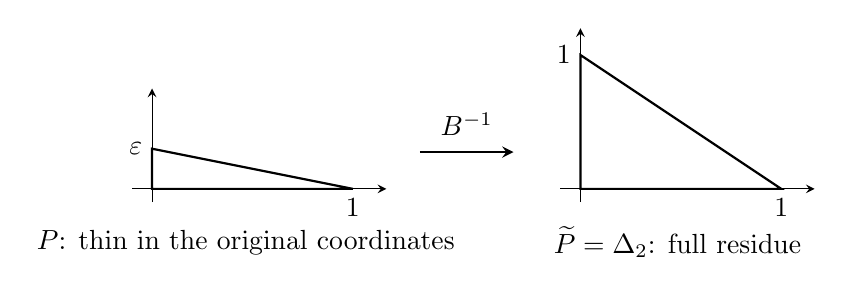
\begin{tikzpicture}[scale=0.85,>=stealth]
 \draw[->] (-0.3,0)--(3.5,0);
 \draw[->] (0,-0.2)--(0,1.5);
 \draw[thick] (0,0)--(3,0)--(0,0.6)--cycle;
 \node[below] at (3,0) {$1$};
 \node[left] at (0,0.6) {$\eps$};
 \node at (1.4,-0.8) {$P$: thin in the original coordinates};
 \draw[->,thick] (4,0.55)--(5.4,0.55);
 \node[above] at (4.7,0.65) {$B^{-1}$};
 \begin{scope}[shift={(6.4,0)}]
 \draw[->] (-0.3,0)--(3.5,0);
 \draw[->] (0,-0.2)--(0,2.4);
 \draw[thick] (0,0)--(3,0)--(0,2)--cycle;
 \node[below] at (3,0) {$1$};
 \node[left] at (0,2) {$1$};
 \node at (1.45,-0.8) {$\widetilde P=\Delta_2$: full residue};
 \end{scope}
\end{tikzpicture}
\caption{Affine normalization of an infinitesimally thin triangle.
The left vertical scale is exaggerated; the picture is schematic, not
a real-scale rendering of an infinitesimal height.}
\end{figure}

\subsection{Cancellation can lie beyond every fixed power scale}
Take $\eta=\omega^{-\omega}$ and $u=(1,1)$, $w=(1,1+\eta)$. Then
\[
 \det(u,w)=\eta.
\]
Keeping only the standard part of each coordinate makes both columns
$(1,1)$ and destroys the determinant. Moreover $0<\eta<\eps^N$ for
every positive integer $N$, so no fixed finite order in powers of $\eps$
reveals it. The correct finite certificate is the determinant itself,
computed with enough exact coefficient information to resolve its
cancellation.

Even in rank one there is no truncation depth depending only on dimension
and vertex count. For each integer $N>0$, the three-vertex triangle with
height $\eps^N$ has nonzero area $\eps^N/2$. A rule discarding all terms
above a fixed power cutoff fails on some such triangle.

\noindent[\wtag{} These two observations are weaker instances of Part~II's
results on coordinate truncation. There, \cref{poly:ts:thm:alternation}
gives four labelled points with coordinates in $\R((\eps))$ whose degree-$N$
truncated hulls alternate between a quadrilateral and a triangle for every
$N$. \cref{poly:ts:thm:universal} realizes \emph{every} prescribed binary
history in the same way. So no truncation depth works, and moreover the
truncated combinatorics need not stabilize at all. Part~I's
\cref{poly:sec:truncation} records the corresponding failure for an exact
algebraic equality. The examples here are kept because they concern a
determinant (a scale) rather than a face lattice.]

\subsection{Identical individual scales do not determine a mixed scale}
Use the rank-two convention
\[
 v\eps=(0,1),\qquad v\eta=(1,0)
 \quad\text{in lexicographically ordered }\Z^2.
\]
Define three parallelograms
\begin{align*}
 P&=[0,e_1]+[0,\eps e_2],\\
 Q&=[0,e_1+\eps e_2]+[0,\eta e_2],\\
 Q'&=[0,\eta e_1]+[0,e_2].
\end{align*}
Their individual areas satisfy
\[
 \Vol_2(P)=\eps,
 \qquad \Vol_2(Q)=\Vol_2(Q')=\eta.
\]
Each is affinely a square, and each has an affine residue affinely
isomorphic to a square. Nevertheless expansion into segments gives
\begin{align*}
 \MV(P,Q)
 &=\tfrac12(\eps+\eta+\eps+0)=\eps+\tfrac12\eta,\\
 \MV(P,Q')
 &=\tfrac12(0+1+\eps\eta+0)=\tfrac12(1+\eps\eta).
\end{align*}
The mixed values are respectively $(0,1)$ and $(0,0)$. Thus individual
volume values and separate affine residue isomorphism classes do not
determine a family's mixed profile. The \emph{relative positions} of its
scale lattices in the common ambient vector space matter.

\subsection{A four-body Pl\"ucker example}
Let
\begin{align*}
 P_1&=[0,e_1]+[0,\eta e_2],&
 P_2&=[0,e_1+\eps e_2]+[0,\eta e_2],\\
 P_3&=[0,e_2]+[0,\eta e_1],&
 P_4&=[0,e_2+\eps e_1]+[0,\eta e_1].
\end{align*}
All four bodies have positive area. Their pure mixed values are
\[
 \tau_{12}=\tau_{34}=v\eps,
 \qquad
 \tau_{13}=\tau_{14}=\tau_{23}=\tau_{24}=0.
\]
(\wtag{} Here $\tau_{ab}=v\MV(P_a,P_b)$ is an entry of the pure profile of
\cref{poly:mv:cor:plucker}; the $\eta$ in the generators is the surreal
$\omega^{-\omega}$, written $\tau$ elsewhere in the report.)
In this example the first displayed generator of each body already gives
a simultaneous inner-segment model. The three Pl\"ucker sums are
$2v\eps,0,0$, so the minimum is attained exactly twice. The example
makes visible the difference between two nearly parallel pairs and the
transverse cross-pairs.

\subsection{The affine residue need not retain all faces}
Let
\[
 P_\eps=\conv\{(0,0),(1,0),(1,1),(0,1),(-\eps,1/2)\}.
\]
It is a pentagon over $K$, of area $1+\eps/2$. Its scale lattice is
$\OO^2$, and its affine residue is the square $[0,1]^2$. Thus a
full-dimensional residue can lose a vertex even though it loses no
dimension. Maximum-simplex normalization does not repair this loss of
fine face information; it is deliberately a first residue invariant.

\noindent[\wtag{} This is the same phenomenon as Part~I's lost-face example
\eqref{poly:ts:eq:lostface} (manuscript~02). There a pentagon has a vertex
infinitesimally below the bottom edge of the rectangle $[-1,1]\times[0,1]$,
and that vertex's standard part is not a face. Here the vertex
$(-\eps,1/2)$ lies infinitesimally outside an edge of the square. The loss
occurs for the standard part and for the affine residue alike: the scale
lattice here is already $\OO^2$, so $\Res(P_\eps)$ is affinely isomorphic to
$\st P_\eps=[0,1]^2$. Part~I's \cref{poly:ts:prop:band} shows how an infinitesimal
optimality band recovers the whole limiting face; see the re-scoped
\cref{poly:mv:q:face-specialization}.]

The real triangle $\Delta_2$ and the real unit square also have the same
scale lattice $\OO^2$, but areas $1/2$ and $1$. The common lattice fixes
the value, not the leading coefficient. This is why a determinant minimum
is an exact scale formula rather than an exact mixed-volume formula.

\subsection{Why the pure/full distinction cannot be dropped}
For $d>1$, a full-dimensional $P$ has $\Vol_d(P)>0$, while every segment
$S$ has $\Vol_d(S)=0$. Therefore no single-segment replacement can
preserve the repeated entry $\MV(P[d])$. The simultaneous theorem is
formulated for \emph{distinct labels} for this reason. The clone theorem
solves the repeated-entry issue by providing independent segment choices
for different copies of the same body.

\subsection{An exact characterization of full profiles}
The clone theorem also has a converse that is useful when formulating
further realization problems.

\begin{corollary}[Full profiles as color-symmetric determinant data]
\label{poly:mv:cor:full-characterization}
An array $t(\alpha)\in\Gamma\cup\{\infty\}$, $|\alpha|=d$, is the full
mixed-volume valuation profile of finite polytopes in $K^d$ if and only if
there is a $d\times md$ matrix over $K$, with $d$ columns of each of $m$
colors, such that every $d$-element column subset $B$ satisfies
\[
 v\det W_B=t(\operatorname{col}(B)).
\]
\end{corollary}
\begin{proof}
Necessity is Theorem~\ref{poly:mv:thm:clones}. For sufficiency, make $Z_i$ the
zonotope generated by the $d$ columns of color $i$. For any $\alpha$,
formula~\eqref{poly:mv:eq:colored-sum} expresses the corresponding mixed volume
as a positive real factor times a finite sum of absolute determinants.
All eligible determinants have value $t(\alpha)$, or all are zero when
$t(\alpha)=\infty$. There is at least one eligible column subset for
every $|\alpha|=d$, since every color has $d$ labels. The positive-sum
lemma gives the required value.
\end{proof}

This is a realizability characterization with matrix witnesses, not a
claim that the exchange axiom alone is sufficient. Removing the matrix
witnesses in favor of a usable intrinsic list of conditions is one of the
research questions below.

\noindent[\wtag{} \Cref{poly:part:trop} re-derives this corollary
independently, as the equivalence (i)$\Leftrightarrow$(iii) of
\cref{poly:trop:thm:polarization}, by generic real block mixing (source~10)
and by integer mixing with the explicit bound $d\binom{dm}{d}$ (source~09,
\cref{poly:fmv:rem:integer-mixing}). Its Fano cubic
(\cref{poly:trop:thm:fano}) shows that exchange-convexity
(\cref{poly:mv:thm:mconvex}, re-proved there by source~09 with the same
nested-clone argument) is not sufficient.]

\section{Finite higher-rank certificates and real specialization}
\label{poly:mv:sec:compression}

\subsection{The finite-support input model}
The preceding results apply to arbitrary finite tuples of elements of
$K$; they are not an algorithm for comparing arbitrary surreal expressions.
For an effective specialization theorem, restrict the coordinates to
finite sums
\[
 f=\sum_{\gamma\in A}a_\gamma t^\gamma,
 \qquad a_\gamma\in\R,
\]
where $A$ is a finite subset of a totally ordered abelian group. Rational
functions in such sums are also allowed when their denominators are
certified nonzero. The order is the Hahn leading-term order: the least
exponent determines the sign and value of a nonzero sum.

A finite certificate may contain coordinate expressions, determinants,
nonzero denominators, polynomial differences encoding comparisons,
and products needed for specified additive comparisons of valuations.
Expand these expressions exactly first; cancellation within an expression
must already have been resolved. For comparisons of absolute determinants,
one may use the polynomial difference of their squares.

\subsection{Finite order data admit an integer-valued model}
\begin{lemma}[Finite positive grading]
\label{poly:mv:lem:grading}
Let $H$ be a finitely generated subgroup of a totally ordered abelian
group, and let $D\subset H_{>0}$ be finite. There exists a group
homomorphism $\lambda:H\to\Z$ with $\lambda(\delta)>0$ for every
$\delta\in D$.
\end{lemma}
\begin{proof}
The group $H$ is finitely generated and torsion-free, so choose an
isomorphism $H\cong\Z^s$. No nontrivial nonnegative integer combination
of members of $D$ can be zero, because all its summands are positive in
$H$.

The origin is not in the real convex hull of the corresponding integer
vectors. Otherwise the finite linear system
$\sum a_\delta\delta=0$, $\sum a_\delta=1$, $a_\delta\ge0$ would
have a real solution and hence a rational solution: a nonempty polytope
defined over $\Q$ has a rational vertex, or a rational point in its
minimal supporting face, by Gaussian elimination. Clearing denominators
would give a forbidden nonnegative integer relation.

Strictly separate this finite convex hull from zero in $\R^s$. The
separating linear functional is positive on all members of $D$. Approximate
its coefficients rationally closely enough to preserve these finitely
many strict inequalities, and clear denominators. The resulting integer
linear functional defines $\lambda$.
\end{proof}

The finite positive-grading principle has a close antecedent in the
repository's support-certificate discussion \cite{mv:RepoReversion}; the
application here is to determinant and polytope sign certificates. It is
not asserted for an infinite support, and it is not asserted to preserve
the full order of $H$.

\begin{theorem}[One-parameter preservation of a finite certificate]
\label{poly:mv:thm:compression}
Let $\mathcal F$ be a finite collection of finite-support Hahn
polynomials. There is an integer-valued homomorphism on the group
generated by their exponents such that the substitution
\begin{equation}
\label{poly:mv:eq:specialization}
 t^\gamma\longmapsto s^{\lambda(\gamma)}
\end{equation}
preserves, for every member of $\mathcal F$, zero versus nonzero, sign,
leading coefficient, and the ordered list of its exponents. It also
preserves the order of the valuations of the nonzero members of
$\mathcal F$. The resulting expressions are ordinary one-variable
Laurent polynomials. Finite rational expressions are covered by including
their nonzero numerators and denominators in the certificate.
\end{theorem}
\begin{proof}
Let $A$ be the union of all supports occurring in $\mathcal F$. Apply
Lemma~\ref{poly:mv:lem:grading} to the positive differences $\beta-\alpha$ of
\emph{all distinct pairs} $\alpha,\beta\in A$ with $\alpha<\beta$.
The resulting homomorphism is strictly order-preserving on the finite
set $A$. Thus no two terms within a certificate polynomial acquire the
same exponent, and the term ordering, leading coefficient, sign, and
nonzeroness are unchanged. Zero expressions remain zero because the
substitution is a group-algebra homomorphism. Comparing leading
exponents across different members gives the assertion about their
valuations. Including denominators ensures that specialization of each
rational expression is defined in $\R(s)$.
\end{proof}

An equality of exponent sums is automatically preserved by a group
homomorphism. To preserve a specified \emph{inequality} between such sums,
include the corresponding products or monomials among the finitely many
certificate expressions before applying the theorem. This prevents an
unwarranted claim that every order comparison in the infinite group has
been retained.

\noindent[\wtag{} \Cref{poly:mv:thm:compression} is the effective,
finite-support counterpart of Part~I's \cref{poly:ts:thm:puiseux}
(manuscript~02). That theorem takes an arbitrary finite bounded
configuration over $K$ and a finite list of polynomial sign conditions. By
real-closed-field transfer and semialgebraic curve selection it gives a
convergent algebraic Puiseux arc over $\R(s)$ that also keeps the prescribed
standard-part limit, but it is not effective. The theorem here assumes
finite-support Hahn input. In exchange it gives an explicit integer
grading, ordinary Laurent polynomials with the same leading coefficients and
exponent order, and the explicit threshold $\rho_g$ below. Part~IV's
\cref{poly:ehr:thm:descent} is a third one-parameter statement, preserving a
whole real trace by algebraic germs. None of the three preserves the entire
higher-rank order (see the example below).]

\subsection{A certified small positive real parameter}
Suppose a nonzero specialized expression is
\[
 g(s)=c_0s^{m_0}+c_1s^{m_1}+\cdots+c_ks^{m_k},
 \qquad m_0<m_1<\cdots<m_k\in\Z.
\]
For $k>0$ set
\[
 \rho_g=\min\left(1,\frac{|c_0|}{2\sum_{j=1}^k|c_j|}\right),
\]
and use $\rho_g=1$ for a single monomial. If $0<s<\rho_g$, then
\[
 \left|s^{-m_0}g(s)-c_0\right|
 \le s\sum_{j=1}^k|c_j|<|c_0|/2,
\]
so $g(s)$ has the sign of its leading coefficient. A common parameter
smaller than all the finitely many thresholds preserves all certificate
signs simultaneously. For rational input coefficients, a rational choice
of $s$ gives a rational finite configuration satisfying those tests.

This result does not contradict non-Archimedean behavior. It reproduces a
\emph{specified finite collection} of inequalities and equalities. It
does not reproduce the assertion $0<\eta<\eps^N$ for every integer $N$.

\begin{example}[Why an entire rank-two order cannot be compressed]
For lexicographic $\Z^2$ with $v\eta=(1,0)$ and $v\eps=(0,1)$, an
order-preserving homomorphism to $\Z$ would have
$a=\lambda(1,0)>N\lambda(0,1)=Nb$ for every $N>0$, with $b>0$.
No two integers $a,b$ satisfy this. In contrast, finitely many comparisons
are preserved by $\lambda(a,b)=Ma+b$ for a sufficiently large integer
$M$. The required $M$ depends on the certificate, not only on the
geometric dimension.
\end{example}

\noindent[\wtag{} This is the same phenomenon as Part~I's
\cref{poly:sec:oneparam} (manuscript~05): the scales $\omega^{-1}$ and
$\omega^{-\omega}$ satisfy $\omega^{-\omega}<\omega^{-N}$ for every $N$, so
replacing them by $t^a,t^b$ with fixed positive real exponents in a
rank-one monomial group cannot preserve all these comparisons. There, as
here, the finite theorems preserve only a specified finite list of
comparisons.]

\subsection{An explicit finite workflow}
A proof-producing implementation for finite-support coordinates can use
the following stages. First establish affine ranks and select maximum
vertex simplices by exact determinant comparisons. Second compute the
mixed determinant lists and their least valuations. Third, when a pure
matrix model is requested, enumerate the rational grids in
Theorem~\ref{poly:mv:thm:segments} and retain a choice passing every determinant
value test. Fourth collect all the resulting finite polynomial tests,
construct a positive grading, and produce a real-parameter sign bound.

The certificate consists of the selected simplex indices, exact
comparison expressions, basis determinants, chosen rational coefficients,
and the finite grading inequalities. Its verification is finite algebra.
The theorem gives a terminating exhaustive-grid method when exact
coefficient and order operations are available. It does not give a
polynomial-time algorithm, a universal truncation depth, or a decision
procedure for unrestricted surreal-number notation.

\section{Exact verification and a formalization route}
\label{poly:mv:sec:verification}

\subsection{What the supplied program actually checks}
The accompanying \pathcode{code/06-affine-residues-verify.py} uses only the Python standard
library. Its coefficient ring is
\[
 \Q[\eta,\eta^{-1},\eps,\eps^{-1}],
\]
with rational coefficients and lexicographically ordered exponent pairs.
Finite sums in this ring embed into the surreal example
$\eta=\omega^{-\omega}$, $\eps=\omega^{-1}$. All sign tests use exact
leading terms; no floating-point arithmetic is used.
(\wtag{} The program and its recorded output name $\eta=\omega^{-\omega}$
\texttt{eta}, for example
\texttt{"exponent\_order": "Z\^{}2 lexicographic, eta=(1,0), epsilon=(0,1)"}
and the key \texttt{lambda\_eta}.)

For planar polytopes, the program computes convex hulls by exact
orientation tests, areas by the shoelace formula, and mixed areas by
polarizing the area of the pairwise-sum convex hull. It then compares
these independently computed mixed areas with the maximum-simplex
mixed-determinant certificate. Thus the audit does not define the mixed
area by the very minimum formula it is checking.

The included report (\pathcode{data/06-affine-residues-verification.json}) records the following run, using seed $20260930$:
\begin{center}
\begin{tabular}{@{}p{0.73\textwidth}r@{}}
\toprule
Audit category & Count\\
\midrule
Random full-dimensional polygon pairs & 160\\
Normalized residue checks from those pairs & 320\\
Scale-lattice/probe equivalence comparisons & 320\\
Exact common-affine-map covariance checks & 24\\
Additional lower-dimensional or zero cases & 4\\
Explicit rank-two mixed-area examples & 2\\
Four-body simultaneous inner-segment families & 20\\
Four-body tropical Pl\"ucker checks & 20\\
Three-color families with six labelled clones & 12\\
Individual $M$-convex exchange tests & 396\\
\bottomrule
\end{tabular}
\end{center}
The program also checks the thin triangle, the cancellation determinant,
the pentagon with square residue, and a finite compression certificate.
Its successful inner-segment choices are searched randomly within the
proved rational grids, with a fixed finite audit budget; that convenience
is distinguished in the source from the exhaustive-grid existence proof.
The run used at most four trials for a four-body family and at most three
for a six-clone family.

To reproduce the default report, run
\begin{verbatim}
python3 code/06-affine-residues-verify.py \
    --output /path/to/scratch/verification.json
\end{verbatim}
(\wtag{} Manuscript~06 printed \texttt{python3 verify.py}. Without
\texttt{--output} the program writes \texttt{verification.json} next to
itself, that is, into \pathcode{code/}; pass an output path outside the
report directory, as above, so that the shipped record is never
overwritten. The delivered \pathcode{code/06-affine-residues-Makefile} still
names the delivery paths \texttt{verify.py} and \texttt{article.tex}.)
The output, shipped as \pathcode{data/06-affine-residues-verification.json}, contains the exact example
expressions, counts, and specialization data. For more instances, the
command-line options \pathcode{--pairs}, \pathcode{--seed}, and
\pathcode{--output} are available. These are finite-instance tests, not a
formal proof of the universal statements and not an exhaustive comparison
with the literature.

\subsection{A modular Lean development}\label{poly:mv:sec:lean-pointer}
\wtag{} The formalization roadmap of manuscript~06 is printed in
\cref{poly:sec:formalization}, together with its statement that the package contains no Lean source and reports no
new Lean build.

\section{Further research questions and topics}
\label{poly:mv:sec:research}

The following questions are proposed directions arising from the proved
results. Their formulation here is not a claim that every item is a
previously published open problem or that no partial answer exists in
related literature. Each question isolates something the current theorems
do not settle.

\begin{question}[Intrinsic full-profile realization]
Give a practical intrinsic characterization of the arrays that admit the
color-symmetric matrix realization of
Corollary~\ref{poly:mv:cor:full-characterization}. Which additional conditions,
beyond support rank constraints and $M$-convex exchange, express
realizability over an ordered field? A useful first target is a complete
analysis for three or four colors in dimension three, keeping the
realization field explicit.
\end{question}
\noindent[\wtag{} \emph{Re-scoped: partly answered in
\cref{poly:part:trop}.} Exchange-convexity with full support, even with
strictly Lorentzian volume polynomials, is not sufficient
(\cref{poly:trop:thm:fano}, $d=3$, seven bodies); every exposed initial
support is a real-representable polymatroid base set
(\cref{poly:trop:thm:initial-support}); every finite-valued $M$-convex
profile with $d=2$ is realizable (\cref{poly:trop:thm:planar}); and a
matroid-type profile is realizable exactly when the matroid is
representable over $\R$ (\cref{poly:trop:thm:matroid-profile}). Dimension
three with three or four colours remains open.]

\begin{question}[Leading coefficients above a fixed scale profile]
Fix a realizable valuation profile $\tau$. Describe the possible positive
leading coefficients of the mixed volumes after choosing a compatible
system of determinant scales. The simultaneous segment theorem determines
the scales but not these coefficients. Can the coefficient problem be
organized by real residue configurations attached to the lowest-valued
minors, rather than by the entire original coordinate series?
\end{question}
\noindent[\wtag{} \emph{Re-scoped: partly answered in
\cref{poly:part:trop}.} Each weighted initial form is the real volume
polynomial of the residue configuration in a minimum-valuation basis
(\cref{poly:trop:thm:initial-polynomial}; unique up to one element of
$\GL_d(\R)$, \cref{poly:fmv:prop:independence}), and a realizable profile
need not have liftable leading coefficients (\cref{poly:fmv:thm:quadratic}).
Compatibility across weights remains open. Source~08's question ``Leading
coefficients beyond valuations'' (\cref{poly:tom:sec:questions}) is the
same question.]

\begin{question}[Joint residue data for several lattices]\label{poly:mv:q:joint-residue}
A single affine residue is full-dimensional, but separate residue shapes
do not determine mixed scales. Construct a canonical finite joint
reduction for a family of embedded scale lattices that retains their
relative position and supports leading-coefficient calculations. For
higher-rank valuations, determine when a finite flag of successive
reductions is sufficient and how its length depends on the family.
\end{question}
\noindent[\wtag{} Related material elsewhere in the report, which leaves
the question open. Part~II's research direction \cref{poly:ts:q:residue}
(manuscript~02) asks for a polyhedral object that keeps the fibres,
infinitesimal widths and near-optimality data discarded by the standard
part; a joint reduction of several scale lattices would be one such object.
Finite flags of successive reductions are proved to suffice in two
narrower settings. For the rows of one halfspace system, Part~IV's
\cref{poly:ehr:thm:lex} needs at most $d+1$ separated real levels per row.
For the heights of a lifting of a fixed real configuration, Part~I's
\cref{poly:thm:pivot} needs at most $n-d-1$ real layers. Neither is a joint
reduction of several scale lattices.]

\noindent[\wtag{} \Cref{poly:fmv:prop:independence} (\cref{poly:part:trop})
gives a common real reduction of a scaled family, canonical up to one
element of $\GL_d(\R)$; the higher-rank flag part remains open.]

\begin{question}[Efficient deterministic inner-segment selection]
The rational grid gives an explicit finite existence bound, but exhaustive
search is generally large. Find a deterministic selection algorithm with
substantially better complexity for the structured product of normalized
determinant polynomials in the proof. Separate arithmetic-operation
complexity from bit complexity of exponents and coefficients, and compare
with the randomized exact search used in the supplement.
\end{question}

\begin{question}[Minimal probe systems]
Theorem~\ref{poly:mv:thm:finite-probes} gives $d+1$ measurements relative to a
reference basis. Determine optimal bounds under various access models:
known reference lattice, unknown basis, restricted directions, and
uniform tests independent of the reference polytope. The distinction
between arbitrary $K$-directions and real directions should be explicit.
\end{question}
\noindent[\wtag{} \emph{Re-scoped.} For uniform tests independent of the
reference polytope the answer is negative in the plane: no fixed finite
family of mixed-area probes recognizes every scale lattice, even with the
area, the spectrum, the shadow and the full residue flag supplied
(\cref{poly:tom:thm:nonadaptive}). Optimality of $d+1$ for the
reference-dependent test remains open.]

\begin{question}[Face specialization and oriented scale data]\label{poly:mv:q:face-specialization}
Characterize when reduction maps faces of $P$ onto faces of $\Res(P)$,
and when vertices or entire face intervals disappear. Enrich the lattice
and residue data by signed leading minors, and compare the resulting
structure with valuated oriented-matroid and regular-subdivision data.
A first useful result would be a finite certificate guaranteeing that
all faces survive a chosen normalization.
\end{question}
\noindent[\wtag{} \emph{Re-scoped: partly answered in this report.} Part~I's
\cref{poly:ts:prop:band} (manuscript~02) shows, for every real functional
$c$, that the standard part of a suitable infinitesimal optimality band
$\{x\in P:c\cdot x\ge M-\eta\}$ is exactly the maximizing face of $\st P$.
So every exposed face of the reduction is recovered from near-optimal points
of $P$, even when the exact maximizing face of $P$ reduces to a nonface
(\eqref{poly:ts:eq:lostface}, and the pentagon in
\cref{poly:mv:sec:examples}). Applied to the bounded normalized polytope
$\widetilde P=B^{-1}(P-p_0)$, whose standard part represents $\Res(P)$
(\cref{poly:mv:thm:affine-residue}), the same identity describes the faces
of the affine residue. Still open: when the faces of $P$ themselves map
onto faces of $\Res(P)$, the signed-minor enrichment, the comparison with
valuated oriented matroids, and the finite survival certificate. Part~II's
research direction \cref{poly:ts:q:residue} (manuscript~02) asks for the
same kind of replacement for the false face map, and cites the same band
identity as its starting point.]

\begin{question}[Adaptive cancellation certificates]
For coordinates supplied as truncatable infinite Hahn series, find
hypotheses under which determinant-leading terms can be certified by an
adaptive terminating procedure. The height-$\eps^N$ examples exclude a
bound depending only on vertex count and dimension. The appropriate
parameters may involve support geometry, coefficient dependencies, or
an input-specific separation certificate rather than a valuation cutoff.
\end{question}
\noindent[\wtag{} Part~II's \cref{poly:ts:thm:universal} (manuscript~02)
sharpens the obstruction. It gives convergent rational power series
coordinates for which the sign of the truncated defect
$1-f_{\le N}g_{\le N}$, which decides the truncated hull type, follows any
prescribed pattern in $N$. So a procedure
that stops once successive truncations agree for a while can be fooled.
The question itself is not answered there.]

\begin{question}[Dual geometric invariants]
Develop mixed-volume and residue invariants involving polar bodies,
widths, and successive directional scales. Simple cube comparisons already
control coarse polar lattices in suitably centered situations; the harder
target is joint leading-coefficient and incidence information under duality,
especially for nonsymmetric bodies and families with different scale
lattices.
\end{question}
\noindent[\wtag{} \emph{Re-scoped.} For centrally symmetric bodies the
coarse polar lattice is exactly the dual module, with reversed spectrum and
$v\Vol(P)+v\Vol(P^\circ)=0$ (\cref{poly:tom:thm:polar}); nonsymmetric bodies
and coefficient-level duality remain open.]

\begin{question}[Beyond finite vertex sets]
Extend the theory to selected definable convex bodies or controlled limits
of polytopes. A satisfactory formulation must first specify the volume
object and its coefficient field: the finite determinant definition does
not automatically extend to arbitrary semialgebraic volume. Determine
which additional hypotheses retain a finite inner-model theorem and which
introduce genuinely infinite residue or support phenomena.
\end{question}
\noindent[\wtag{} \emph{Re-scoped: partly answered.} \Cref{poly:part:bf}
treats set-sized presentations: a class that is both a set-generated hull
and a set-indexed halfspace intersection has finite subpresentations of
both (\cref{poly:bf:thm:rigidity}), so definable small hulls are polytopes;
the volume half of this question is untouched.]

\begin{question}[Formal certificates in the repository]
Implement and independently check the maximum-simplex module theorem,
the mixed determinant squeeze, and the simultaneous grid theorem as
separate generic Lean modules. Connect finite-support computational
certificates to those statements without assuming unrestricted comparison
of surreal expressions. The concrete goal is an auditable end-to-end
example in which a higher-rank mixed-volume profile is verified from
vertex data and then instantiated in the constructed surreal field.
\end{question}

\section{Conclusion}
The finite face lattice alone does not distinguish real from surreal
polytope geometry. The first meaningful extra layer is the embedded
scale lattice; a maximum vertex simplex makes it explicit and supplies a
full-dimensional affine residue. The scale of every mixed volume is then
a finite determinant minimum.

The simultaneous inner-segment theorem adds a global compatibility fact:
all pure mixed-volume scales of a finite family come from one matrix.
The clone construction extends this compatibility to repeated entries and
produces the full exchange axiom over arbitrary ordered value groups.
These results give exact simplification and reconstruction statements,
while the examples identify what they deliberately forget: residue
coefficients, fine faces, and unrestricted higher-order information.

The resulting research program is finite and algebraic at its core.
It can use the surreal field to accommodate very large hierarchies of
scales without relying on class-sized measure theory or on a nonexistent
universal real-valued parameter. Its next substantive challenge is to
recover the coefficient and incidence geometry above those scale data,
not merely to reprove the ordinary finite combinatorics over a larger field.

\section{Proof dependencies and audit boundaries (Appendix~A of manuscript~06)}
\label{poly:mv:app:audit}

The main scale results have the following dependency chain:
\[
\begin{gathered}
 \text{finite maximum simplex and Cramer's rule}\\
 \Downarrow\\
 L(P)=B\OO^r\quad\text{and the parallelotope sandwich}\\
 \Downarrow\\
 \text{mixed determinant minimum and intrinsic determinant ideal}\\
 \Downarrow\\
 \text{finite residue-polynomial avoidance and simultaneous segments}\\
 \Downarrow\\
 \text{clone realization and determinant exchange}\\
 \Downarrow\\
 \text{full-profile }M\text{-convexity over }\Gamma.
\end{gathered}
\]
The affine residue and its leading-volume identity use the separate
standard-part volume lemma. The probe classification uses the determinant
ideal and the adjugate formula, not the genericity argument. Finite
one-parameter specialization is an additional effective result for
finite-support coordinates; it is not needed for any existence theorem
about arbitrary finite surreal coordinates.

\begin{center}
\begin{tabular}{@{}p{0.27\textwidth}p{0.66\textwidth}@{}}
\toprule
Potential failure mode & How the statements handle it\\
\midrule
Proper-class domain & All inputs and constructions are placed in a
set-sized real closed subfield of $\No$.\\[0.45em]
Lower-dimensional body & Its module has its affine rank; a point argument
makes the mixed volume zero. Support is decided by
Corollary~\ref{poly:mv:cor:support}.\\[0.45em]
Infinite or infinitesimal size & Maximum-simplex coordinates put the body
in a real bounded cube without changing its affine rank.\\[0.45em]
Cancellation & Determinants are computed exactly. Generic segment
selection avoids the finitely many leading cancellations simultaneously.\\[0.45em]
Higher-rank value group & Proofs use finite comparisons and real residue
polynomials, never cofinal multiples of a positive value.\\[0.45em]
Repeated arguments & One segment per original body is insufficient;
parallelotope models or separately labelled clones are used.\\[0.45em]
Unjustified transfer & Only fixed finite polytope formulas and their
semialgebraic determinant volumes are transferred.\\[0.45em]
Overstated effectiveness & Algorithms assume exact finite-support
arithmetic. Arbitrary surreal comparison and polynomial-time bounds are
not claimed.\\[0.45em]
Overstated novelty & Classical ingredients are credited. The combined
results are research proofs supplied for review, not certified historical
priority claims.\\
\bottomrule
\end{tabular}
\end{center}


\part{Real traces and lattice-point counting}\label{poly:part:ehr}

\paragraph{Source and scope.}\wtag{} This Part prints, whole, manuscript~03 of
batch~58: \emph{Infinitesimal Boundary Geometry of Surreal Polytopes:
Lexicographic traces, one-parameter descent, and Ehrhart universality}, headed
``Surreal geometry / lattice enumeration'', author line ``Research manuscript
prepared for Vladimir Reshetnikov'' (the PDF metadata of the delivered file
reads ``Research manuscript prepared with ChatGPT''), dated September~30, 2026
(archive \pathcode{surreal_polytope_research.zip}, main file
\pathcode{surreal_polytopes/surreal_polytopes.tex}; delivered PDF of 28 pages
on Letter paper, not shipped). It was written against ProveIt commit
\pathcode{6996fee43}. Every section, result, proof, example, remark, figure,
table and research question of the manuscript is printed here, in the
manuscript's order, with three structural changes: its two appendices are
printed as the ordinary \cref{poly:ehr:app:scope,poly:ehr:app:ledger}; its
subsection ``A realistic formalization sequence'' is printed in the
formalization chapter (\cref{poly:ehr:sec:formalization}); and its
bibliography is printed as the list ``References of Part~IV''. This Part is
its own spine (\cref{poly:sec:guide}): it shares no theorem with the other
Parts beyond two foundations, both marked where they occur. These are the
shadow of a finite hull (\cref{poly:ehr:lem:shadow}, proved in Part~I as
\cref{poly:prop:stconv}) and finite real-closed-field transfer
(\cref{poly:ehr:prop:transfer}; Part~I's \cref{poly:thm:general} and Part~V's
\cref{poly:ic:thm:conservativity}). The Part keeps its own definitions and
hypotheses, fixed in \cref{poly:ehr:sec:setup}. In this Part ``the article''
and ``this manuscript'' mean manuscript~03. As in Part~III, every
theorem is stated for an arbitrary set-sized real closed field $K\supseteq\R$
with no rank or valuation hypothesis; the surreal field supplies the
examples and, through bounded omnific integers, the reason for counting
ordinary lattice points.

\paragraph{Notation in this Part.}\wtag{} The following symbols mean something
different elsewhere in the report (\cref{poly:sec:notation}); the Part-local
meaning is the one in force here. No symbol of manuscript~03 has been renamed.
\begin{itemize}
\item $\mathcal O_K$ and $\mathfrak m_K$ are the finite elements and the
  infinitesimals: the same ring and ideal as $\cO_K$ (Parts~I--II) and $\OO$,
  $\mm$ (Parts~III and~V). $\st$ is the standard part, and the \emph{shadow}
  $Q=\st(P)$ is the standard part of the polytope, as in Part~I.
\item The \emph{real trace} $S=\Tr(P)=P\cap\R^d$ (printed $\operatorname{Tr}_{\R}$)
  is the set of real points of $P$. It is \emph{not} the shadow: it can be
  empty or non-closed while the shadow is a full polytope
  (\cref{poly:ehr:ex:lowdim}); in general $\intr Q\subseteq S\subseteq Q$
  only for a full-dimensional shadow. Nor is it Part~V's matrix trace $\tr$,
  or Part~III's affine residue $\Res$.
\item $L_P(n)=\#(nP\cap\Z^d)$ counts lattice points; it is unrelated to
  Part~III's scale lattice $L(P)$ and to Part~I's $L_h$. $\Oz$ is the ring of
  omnific integers.
\item $\eps$ and $\delta$ denote an \emph{arbitrary} positive infinitesimal of
  $K$, not necessarily $\omega^{-1}$; $t$ is a real parameter tending to $0^+$,
  or the positive infinitesimal of the ordered field $\R(t)$ (not Part~II's
  $t=\omega^{-1}$); $\eta>0$ in \cref{poly:ehr:thm:descent} is a \emph{real}
  cutoff for that parameter (not Part~I's sign threshold, not
  $\tau=\omega^{-\omega}$).
\item $\rho_1\gg\cdots\gg\rho_r$ is a separated basis of positive elements of
  a real subspace of $K$ (\cref{poly:ehr:lem:separated}); it is not Part~V's
  monomial $\rho$ or Part~III's threshold $\rho_g$.
\item $m$ is the number of rows in \cref{poly:ehr:thm:lex}, a period in the
  proof of \cref{poly:ehr:thm:quad}, and a nonsquare integer in
  \cref{poly:ehr:sec:verification} (not Part~III's number of bodies);
  $S$, $T$, $G$, $Q$, $B$, $E$, $H$ are the trace, an implanted real polytope,
  a face, the shadow, a bounding box, a realization space or generating
  function, and a halfspace intersection or generating function (not Part~V's
  slack matrix $S$ or triangle $T$); $A(Q)$ is the lattice-normalized boundary
  measure and $\mu_F$ the normalized facet measure; $V_i$ are coefficient
  spaces (not Part~I's dependence space); $\beta(P)$ is the surface
  coefficient.
\item $\vol_d$ is Euclidean volume of real sets; on real polytopes it agrees
  with Part~III's determinant volume $\Vol_d$.
\item No valuation is used in this Part (see the remark after
  \cref{poly:ehr:thm:descent}).
\end{itemize}

\paragraph{Abstract of manuscript 03.}
A finite surreal polytope has an ordinary realizable face lattice, but its
infinitesimal boundary placement can carry arithmetic information invisible
in that lattice and in its standard-part shadow. We give a finite
lexicographic description of its real trace, with at most $d+1$ levels per
inequality in dimension $d$. Combining this description with semialgebraic
curve selection gives a one-parameter algebraic realization preserving the
entire real trace, the shadow, the labeled face lattice, and every ordinary
lattice-counting value. We then construct a face-implantation operation that
imports arbitrary lower-dimensional real-polytope counting functions into a
fixed rational shadow. For a lattice shadow, we prove an explicit second
asymptotic coefficient and determine its full attainable interval. If the
shadow is simple, every value in this interval is attained without changing
the labeled face lattice or any vertex standard part. Finally, a quadrilateral
with the four integral vertex shadows of the unit square has counting function
$(n+1)^2-\lceil\alpha n\rceil$ for any irrational $0<\alpha<1$; its generating
function has the unit circle as a natural boundary and is not D-finite.

\paragraph{Status and scope (title page of manuscript 03).} This manuscript supplies mathematical
proofs and exact finite checks. It has not been independently refereed or
formalized in Lean. Its classical inputs are explicitly attributed; priority
for the assembled results is not certified. No named published open conjecture
is claimed solved. All counting statements concern ordinary integer dilations
of polytopes bounded by a real box.


\section{The research questions and their answers}\label{poly:ehr:sec:introduction}

The relevant starting point in \repo\ is its construction of the surreal
field and its omnific-integer subring, together with its distinction between
research manuscripts and mapped formal theorems \cite{ehr:repo-readme,ehr:repo-guide}.
The particularly useful bridge is that an omnific integer bounded in absolute
value by a real number is an ordinary integer. The repository contains an
explicit Lean declaration of this statement \cite{ehr:repo-units}. Consequently,
finite polytopes in bounded surreal space lead to a precise, ordinary
lattice-enumeration problem. Their coordinates may be non-Archimedean; the
lattice points being counted are not.

The organizing question is not whether arbitrary finite combinatorics becomes
possible over the surreals. Real-closed-field transfer already rules that out
for finite face lattices. Rather, we ask what information survives when one
retains the real numbers and their integer lattice while moving supporting
hyperplanes through infinitesimal distances.

\subsection{Four questions posed and resolved here}

\paragraph{Does the shadow determine lattice enumeration?}
No. Even a surreal quadrilateral with exactly the four integral vertex shadows
of the unit square can have non-quasipolynomial counts. Its generating
function can have infinitely many analytic obstructions in the strongest
possible form: every point of the unit circle is a singular boundary point.
The construction and proof appear in Section~\ref{poly:ehr:sec:quad}.

\paragraph{Can arbitrarily deep surreal scales be necessary for the real trace?}
Not for a finite system in fixed dimension. An individual affine inequality
in $d$ coordinates needs at most $d+1$ lexicographic levels on real inputs.
A stronger global theorem replaces the whole polytope by one algebraic
parameter while preserving its trace and finite combinatorics simultaneously;
see Sections~\ref{poly:ehr:sec:lex}--\ref{poly:ehr:sec:descent}. This is a statement about a
specified finite geometric object, not about collapsing the surreal field
or its full value group.

\paragraph{How much counting behavior can be hidden on a face?}
Every real polytope lying in that face can be implanted. If $G$ is a proper
face of a rational polytope $Q$ and $T\subseteq G$ is any real polytope, we
construct $P$ with shadow $Q$ and
\[
 L_P(n)=L_Q(n)-L_G(n)+L_T(n)\qquad(n\geq1).
\]
The last summand need not be an Ehrhart quasipolynomial. This isolates a
universality mechanism rather than merely an isolated counterexample.

\paragraph{What remains of the first two Ehrhart coefficients?}
For a full-dimensional lattice shadow $Q$, the leading coefficient is always
$\vol_d(Q)$. The next coefficient is the sum of the normalized measures of
the portions of facets retained in the real trace, minus half the normalized
boundary measure of $Q$. Its complete attainable interval is
\[
 \left[-\frac12\sum_F\mu_F(F),\;
        \frac12\sum_F\mu_F(F)\right].
\]
For a \emph{simple} lattice shadow every value is attainable by perturbing its
existing facets, with no change in the labeled face lattice and no change in
any vertex standard part. Sections~\ref{poly:ehr:sec:surface} and \ref{poly:ehr:sec:interval}
prove these statements.

\subsection{What is classical, and what is being assembled}

The real-closed-field transfer principle and semialgebraic curve selection
are classical \cite{ehr:bpr,ehr:basu-roy,ehr:fernando}. Lexicographic inequalities are
also established objects in optimization \cite{ehr:lex-cuts}. Classical Ehrhart
theory and reciprocity apply to rational polytopes \cite{ehr:sam-woods}.
Irrationality does not by itself preclude polynomial enumeration: period
collapse already occurs for irrational triangles \cite{ehr:cgls}. Finally,
the natural-boundary step below is an application of the classical
P\'olya--Carlson theorem, not a new complex-analytic theorem
\cite{ehr:bell-et-al}.

The contributions developed here are the finite trace normal form and its
trace-preserving descent application, the face-implantation construction,
the surface-coefficient formula and its sharp realization theorem, and the
explicit connection of these statements to bounded surreal and omnific
geometry. Their proofs are given in full, except for the clearly named
classical inputs. These results may overlap consequences of existing
non-Archimedean convexity or real-algebraic geometry; the literature checks
recorded here are not an exhaustive priority search.

\section{Fields, finite polytopes, shadows, and traces}\label{poly:ehr:sec:setup}

\subsection{A set-sized setting}

Throughout, $K$ is a set-sized real closed ordered field containing $\R$ as
an ordered subfield. When an infinitesimal is needed we suppose that
$0<\eps<r$ for every $r\in\R_{>0}$. Define
\[
 \mathcal O_K=\{x\in K:|x|\leq r\text{ for some }r\in\R_{>0}\},
 \qquad
 \mathfrak m_K=\{x\in K:|x|<r\text{ for every }r\in\R_{>0}\}.
\]
Completeness of $\R$ gives a unique standard part
$\st(x)\in\R$ for $x\in\mathcal O_K$, characterized by
$x-\st(x)\in\mathfrak m_K$. To see existence, take the supremum of the real
numbers below $x$; the defining property of the supremum excludes a positive
real distance in either direction. Uniqueness follows because no nonzero
real number is infinitesimal. Directly from this characterization,
\[
 \st(x+y)=\st(x)+\st(y),\qquad
 \st(xy)=\st(x)\st(y),
\]
and $x\geq0$ implies $\st(x)\geq0$. Thus $\mathcal O_K$ is a convex subring,
$\mathfrak m_K$ is its maximal ideal, and its residue field is $\R$.

A finite tuple of surreal coordinates can be placed in such a field: take
inside $\No$ the real closure of the field generated by $\R$ and that tuple.
This uses the classical real closedness of the surreal field
\cite{ehr:gonshor}. All constructions below take place in this set-sized field.
No application of first-order model theory treats the proper class $\No$
as a set-sized structure, and no saturation hypothesis is used.

\begin{definition}
A \emph{finite $K$-polytope} is the convex hull of finitely many points of
$K^d$, with convex combinations using nonnegative coefficients in $K$.
It is \emph{real-bounded} if it is contained in $[-M,M]^d$ for some
$M\in\R_{>0}$. For such a nonempty polytope $P$, its \emph{shadow} and
\emph{real trace} are
\[
 Q=\st(P)=\{\st(x):x\in P\}\subseteq\R^d,
 \qquad S=\Tr(P)=P\cap\R^d.
\]
Standard part is applied coordinatewise.
\end{definition}

Finite-dimensional polyhedral linear algebra works over real closed fields.
In particular a finite convex hull has a finite halfspace representation,
allowing pairs of opposite inequalities to encode its affine hull, and a
nonempty bounded intersection of finitely many closed halfspaces is a finite
convex hull. These statements can be obtained from finite elimination, or
from their fixed-size first-order real versions by transfer
\cite{ehr:bpr}. We never invoke topological compactness of a bounded subset of
$K^d$.

\begin{lemma}[The shadow of a finite convex hull]\label{poly:ehr:lem:shadow}
If $P=\conv_K(v_1,\ldots,v_N)$ is real-bounded, then
\[
 \st(P)=\conv_\R\bigl(\st(v_1),\ldots,\st(v_N)\bigr).
\]
In particular, its shadow is an ordinary closed real polytope.
\end{lemma}
\begin{proof}
If $x=\sum_j\lambda_jv_j$ with $\lambda_j\geq0$ and
$\sum_j\lambda_j=1$, then every $\lambda_j$ is finite and its standard
part is nonnegative. Taking standard parts produces a real convex
combination. Conversely, a real convex combination of the shadow vertices
is the standard part of the same real combination of their lifts.
\end{proof}

\noindent[\wtag{} This is Part~I's \cref{poly:prop:stconv}, where it is
proved (manuscripts 05 and 02), and the first clause of Part~III's
\cref{poly:mv:lem:hull-reduction}. Manuscript~03's statement and proof are
kept because the rest of this Part cites them.]

\begin{lemma}[Interior points survive]\label{poly:ehr:lem:interior}
If $Q=\st(P)$ has dimension $d$, then
\[
 \intr Q\subseteq S\subseteq Q,
 \qquad\cl_\R S=Q.
\]
\end{lemma}
\begin{proof}
The second inclusion is immediate because $\st(x)=x$ for real $x$.
For $x\in\intr Q$, choose a real $d$-simplex in $Q$ containing $x$ in its
interior. Its vertices $q_0,\ldots,q_d$ have lifts
$p_0,\ldots,p_d\in P$ by Lemma~\ref{poly:ehr:lem:shadow}. The matrix whose columns
are $(1,p_j)$ has determinant with nonzero standard part. It is therefore
invertible over $K$. The solution of
\[
 \sum_{j=0}^d\lambda_jp_j=x,\qquad \sum_{j=0}^d\lambda_j=1
\]
has standard part equal to the strictly positive barycentric coordinates
of $x$ in the real simplex. Hence every $\lambda_j>0$, so $x\in P$.
Taking closures gives the last assertion.
\end{proof}

\begin{example}[A shadow is not a trace]\label{poly:ehr:ex:lowdim}
The segment $\{(x,\eps):0\leq x\leq1\}$ has shadow
$[0,1]\times\{0\}$ and empty real trace. Thus the dimension assumption in
Lemma~\ref{poly:ehr:lem:interior} cannot be dropped. Even for full-dimensional
shadows the trace need not be closed: $[\eps,1-\eps]$ has trace $(0,1)$
and shadow $[0,1]$.
\end{example}

\subsection{Ordinary and omnific lattice points}

Conway's omnific integers are the surreal normal forms with no negative
exponents and with an ordinary integer constant coefficient
\cite{ehr:gonshor}. A nonconstant such form has a nonzero leading term of
positive exponent, so it is not bounded in absolute value by a real number.
It follows that
\begin{equation}\label{poly:ehr:eq:finite-oz}
 \Oz\cap\mathcal O_{\No}=\Z.
\end{equation}
This is also the content of the repository theorem
\texttt{omnific\_bounded\_iff}; Section~\ref{poly:ehr:sec:repo} records the exact path
and the verification boundary \cite{ehr:repo-units}.

\noindent[\wtag{} \texttt{omnific\_bounded\_iff} is the one Lean
declaration that any Part of this report uses as an input; the other Parts
cite Lean declarations at most as background. It states that an omnific
integer whose surreal value is bounded in absolute value by a real number
is the cast of an ordinary integer. Re-verified at the write phase: it is
at line~65 of
\pathcode{Algebra/SurrealNumbers/Surreal/Foundations/OmnificUnits.lean}, in
namespace \texttt{Surreal.Foundations.SignSequence}, next to
\texttt{omnific\_isFinite\_iff} (line~55) and
\texttt{omnific\_eq\_intConstant\_of\_finite} (line~42), and the file is
unchanged since the pin. Manuscript~03 also proves \eqref{poly:ehr:eq:finite-oz}
directly from normal forms, as above. \emph{None of this Part's own results
is formalized}: the Lean statement covers only the bridge
\eqref{poly:ehr:eq:finite-oz}, not the trace, descent, implantation,
counting or surface-coefficient theorems.]

For any real-bounded $K$-polytope and an \emph{ordinary} positive integer
$n$, define $L_P(n)=\#(nP\cap\Z^d)$. In the surreal case,
\begin{equation}\label{poly:ehr:eq:count}
 L_P(n)=\#(nP\cap\Oz^d)=\#(nP\cap\Z^d)=\#(nS\cap\Z^d).
\end{equation}
The omnific and integer sets agree coordinatewise by
\eqref{poly:ehr:eq:finite-oz}; the last equality holds over any $K$ because
$x/n\in\R^d$ for real $x$.
The counts are finite, and we set $L_P(0)=1$ for nonempty $P$.
For a real polytope or bounded real set $T$, write
$L_T(n)=\#(nT\cap\Z^d)$ when the ambient space is understood.

Equation~\eqref{poly:ehr:eq:count} is a reduction to the \emph{real trace}, not to
the shadow. It also explains why the integer-part structure does not add
new bounded lattice points. Infinite omnific dilations, infinite-coordinate
polytopes, and counts indexed by a proper class are outside our scope.

\section{The classical limit: no new finite face lattices}\label{poly:ehr:sec:transfer}

\begin{proposition}[Finite combinatorial transfer]\label{poly:ehr:prop:transfer}
Every finite polytope over a real closed ordered field has a realization over
the real algebraic numbers with the same labeled vertex--facet incidences,
and consequently the same face lattice. Real boundedness is not required.
\end{proposition}
\begin{proof}
Choose a finite vertex list and a finite inequality description, including
affine-hull equations when necessary. With their sizes fixed, the following
requirements form a finite first-order formula in the language of ordered
fields: the convex hull equals the halfspace intersection; the listed points
are pairwise distinct vertices; and each specified vertex--row slack is zero
or strictly positive according to the original incidence data. Convex-hull
membership is expressed with finitely many existential barycentric
coordinates. Extremality is expressed by exclusion from the convex hull of
the other listed vertices. H/V equality is expressed by quantifying a point
of the fixed ambient dimension. None of these formulas names a nonrational
parameter: all coordinates and coefficients are variables.

The formula has a solution in the given real closed field. Completeness of
the theory of real closed fields gives a solution in the real algebraic
numbers \cite{ehr:bpr}. Every face of a polytope is an intersection of its
supporting facets, so the preserved incidence data determine the labeled
face lattice. Equivalently one can transfer the finite determinant sign
pattern of a homogeneous vertex configuration.
\end{proof}

This observation prevents a misleading research claim: finite surreal
polytopes do not create previously unrealizable finite face lattices.
It does not say that all face lattices have rational realizations, that
given coordinates descend, or that standard parts and valuations are
preserved. Most importantly, quantification over $\Z$ is not part of the
pure ordered-field language. Proposition~\ref{poly:ehr:prop:transfer} gives no
transfer theorem for lattice-counting functions.

\noindent[\wtag{} \Cref{poly:ehr:prop:transfer} is the finite
real-closed-field transfer that Part~I proves as \cref{poly:thm:general}
(manuscripts 05 and 02); Part~III's \cref{poly:mv:prop:faces} is another
instance. Part~V's \cref{poly:ic:thm:conservativity} (manuscript~07)
strengthens it for polytopes over a real closed field: a real-algebraic
realization can keep the oriented matroid and the linear and semidefinite
extension complexities as well. The limitations just stated apply to all of
these: none transfers standard parts, valuations or lattice counts.]

The rest of this article retains exactly the data discarded by that
proposition: the distinguished real subfield, its standard-part map, and
the boundary trace on the ordinary integer lattice.

\section{A finite lexicographic normal form for real traces}\label{poly:ehr:sec:lex}

For positive $a,b\in K$, write $a\gg b$ if $b/a$ is infinitesimal.
For a finite tuple of real numbers, lexicographic nonnegativity means either
that every entry is zero or that its first nonzero entry is positive.

\begin{lemma}[Separated real basis]\label{poly:ehr:lem:separated}
Let $V\subseteq K$ be a nonzero real vector space of finite dimension $r$.
There is a basis of positive elements
\[
 \rho_1\gg\rho_2\gg\cdots\gg\rho_r>0
\]
such that, for all $c_1,\ldots,c_r\in\R$,
\[
 \sgn\left(\sum_{j=1}^r c_j\rho_j\right)
 =\sgn(c_k)
\]
when $k$ is the first index with $c_k\ne0$.
\end{lemma}
\begin{proof}
Choose a real basis $v_1,\ldots,v_r$ and let $\rho_1$ be the largest of
$|v_1|,\ldots,|v_r|$. It belongs to $V$, is positive, and every $v/\rho_1$
with $v\in V$ is finite: the coefficients of a fixed finite real linear
combination give a real bound. Therefore
\[
 c_1:V\longrightarrow\R,\qquad c_1(v)=\st(v/\rho_1)
\]
is real linear and takes $\rho_1$ to $1$. Its kernel has dimension $r-1$,
and every element of the kernel is infinitesimal relative to $\rho_1$.
Moreover,
\[
 V=\R\rho_1\oplus\ker c_1.
\]
Apply the same argument inside the kernel. Induction gives an exact basis
expansion after $r$ steps. Each later basis element divided by an earlier
one is infinitesimal. After dividing a nonzero combination by its first
active $\rho_k$, its leading coefficient is a nonzero real number and the
remaining finite sum is infinitesimal. This proves the sign rule.
\end{proof}

This argument uses exact finite-dimensional linear algebra. It does not
truncate a Hahn series, assume that its support is finite, or require that
the value group have finite rank.

\begin{theorem}[Lexicographic trace theorem]\label{poly:ehr:thm:lex}
Let
\[
 P=\{x\in K^d:b_i-a_i\cdot x\geq0,\ 1\leq i\leq m\}
\]
be any finite halfspace system. For every nonzero row there exist real affine
forms $\ell_{i1},\ldots,\ell_{ir_i}$, where $r_i\leq d+1$, such that
\begin{equation}\label{poly:ehr:eq:lex-trace}
 P\cap\R^d=
 \{x\in\R^d:(\ell_{i1}(x),\ldots,\ell_{ir_i}(x))\lexge0
                      \text{ for all }i\}.
\end{equation}
More precisely, there are positive separated scales $\rho_{ik}$ with
\begin{equation}\label{poly:ehr:eq:row-expansion}
 b_i-a_i\cdot x=\sum_{k=1}^{r_i}\rho_{ik}\ell_{ik}(x)
                    \qquad(x\in K^d).
\end{equation}
Zero rows may be deleted.
\end{theorem}
\begin{proof}
Apply Lemma~\ref{poly:ehr:lem:separated} to
\[
 V_i=\operatorname{span}_\R\{b_i,a_{i1},\ldots,a_{id}\}.
\]
Its dimension is at most $d+1$. Expand each coefficient in the separated
basis and collect the real affine forms multiplying the basis elements.
This gives the exact identity \eqref{poly:ehr:eq:row-expansion}. When $x$ is real,
all $\ell_{ik}(x)$ are real, so the sign rule is precisely
\eqref{poly:ehr:eq:lex-trace}.
\end{proof}

\begin{corollary}[Finite semilinear structure]\label{poly:ehr:cor:semilinear}
The real trace of a real-bounded finite $K$-polytope is a convex semilinear
set. It is a finite disjoint union of relatively open real polytopes.
\end{corollary}
\begin{proof}
A lexicographic condition is a finite union of conditions of the form
\[
 \ell_1=\cdots=\ell_{k-1}=0,\quad\ell_k>0,
\]
together with the all-zero condition. Thus it is semilinear. Subdivide a real
bounding box by all the affine hyperplanes in the description and by its
boundary hyperplanes. Each relatively open cell has a constant truth value
for the trace formula. The selected cells give the stated finite disjoint
union; boundedness makes their closures polytopes. Convexity follows from
convexity of $P$ and the real subfield.
\end{proof}

\begin{example}[Why leading standard parts are insufficient]
The inequality
\[
 1-y+\eps(x-\alpha)\geq0
\]
on real $(x,y)$ first tests $1-y$. Only on the line $y=1$ does it test
$x-\alpha$. Taking the standard part of its coefficients loses the second
test and incorrectly keeps the entire line segment on that boundary.
\end{example}

\subsection{Polynomial compression, without a combinatorial guarantee}

\begin{corollary}[A degree-$d$ one-infinitesimal trace description]
\label{poly:ehr:cor:flat}
Suppose $P$ is real-bounded and its shadow is full-dimensional. Fix a real
bounding box $B$ containing $P$. For any positive infinitesimal $\delta$,
set
\[
 P_{\rm flat}=\left\{x\in B_K:
       \sum_{k=1}^{r_i}\delta^{k-1}\ell_{ik}(x)\geq0\quad\text{for all }i
                   \right\}.
\]
Then $P_{\rm flat}$ is a nonempty real-bounded polytope with the same real
trace and shadow as $P$. Its row coefficients are polynomials in $\delta$
of degree at most $d$. In the surreal setting all its ordinary counting
values agree with those of $P$.
\end{corollary}
\begin{proof}
On real inputs powers of $\delta$ implement exactly the same lexicographic
sign rule. Thus the traces agree. The common trace contains $\intr Q$ by
Lemma~\ref{poly:ehr:lem:interior}, so $P_{\rm flat}$ is nonempty and its shadow is
full-dimensional. Applying that lemma to both polytopes shows that both
shadows are the closure of the common trace. Equation~\eqref{poly:ehr:eq:count}
proves the counting claim.
\end{proof}

This compression need not preserve the original face lattice. Different
rows may interact through their relative infinitesimal scales at nonreal
points. The next theorem preserves those interactions by selecting an
algebraic curve in an appropriate realization space rather than replacing
each row independently.

\section{One-parameter algebraic descent preserving the entire trace}
\label{poly:ehr:sec:descent}

An \emph{algebraic semialgebraic germ} below is a germ at $t=0^+$ of a real
semialgebraic function algebraic over $\R(t)$. It can be chosen Nash on a
sufficiently small positive interval. The coefficients of its defining
polynomial may be arbitrary real numbers; ``algebraic'' here does not mean
``defined over $\Q$.''

\begin{theorem}[Trace-preserving algebraic descent]\label{poly:ehr:thm:descent}
Let $P\subseteq K^d$ be a nonempty real-bounded finite polytope, with its
distinct vertices labeled $v_1,\ldots,v_N$. There exist $\eta>0$ and a family
of ordinary real polytopes $P_t$, $0<t<\eta$, whose labeled vertices and
inequality coefficients are algebraic semialgebraic germs, such that:
\begin{enumerate}[label=(\roman*)]
\item every $P_t$ has the same labeled vertex--inequality incidences and face
      lattice as $P$;
\item its labeled vertices $v_j(t)$ tend to $\st(v_j)$;
\item for every fixed real point $x$, membership $x\in P_t$ is eventually
      constant and equals membership $x\in\Tr(P)$.
\end{enumerate}
Evaluating these germs at a positive infinitesimal gives a polytope $P^*$
in a real closure of $\R(t)$, embedded in a real closed extension, with
exactly the same real trace, shadow, and labeled face lattice as $P$.
All ordinary lattice counts agree. For every fixed ordinary $n\geq1$,
\[
 L_{P_t}(n)=L_P(n)
\]
for all sufficiently small positive real $t$, where the cutoff may depend
on $n$. No full-dimensional-shadow hypothesis is needed.
\end{theorem}

\begin{proof}
We give the finite encoding because preserving all real points at once is
stronger than preserving a finite determinant sign list.

\paragraph{Step 1: encode every row with adjacent ratios.}
Use the exact expansion \eqref{poly:ehr:eq:row-expansion} and divide row $i$ by its
positive $\rho_{i1}$. Introduce one variable $u_{ik}$ for each adjacent
ratio, and write
\begin{equation}\label{poly:ehr:eq:row-u}
 f_i(u,x)=\ell_{i1}(x)+u_{i1}\ell_{i2}(x)
 +u_{i1}u_{i2}\ell_{i3}(x)+\cdots
 +(u_{i1}\cdots u_{i,r_i-1})\ell_{ir_i}(x).
\end{equation}
The original ratio tuple $u^0_{ik}=\rho_{i,k+1}/\rho_{ik}$ consists of
positive infinitesimals. Substituting it recovers the original normalized
rows exactly. Choose a closed real box $B$ containing $P$ strictly inside
its boundary.

\paragraph{Step 2: construct a semialgebraic realization space.}
Let $z=(z_1,\ldots,z_N)$ be variable points. Let $E$ be the set of real
pairs $(u,z)$ satisfying the following finite first-order conditions:
$0<u_{ik}<1$; all $z_j\in B$; the polyhedron
\[
 H(u)=\{x\in B:f_i(u,x)\geq0\text{ for every }i\}
\]
equals $\conv(z_1,\ldots,z_N)$; the $z_j$ are distinct and each lies outside
the convex hull of the others; and each slack $f_i(u,z_j)$ is zero or
strictly positive according to the original row--vertex table. The box
inequalities can be included in this table as well.

H/V equality and exclusion from a finite convex hull have first-order
formulas with finitely many barycentric variables. Quantifier elimination
therefore makes $E$ a semialgebraic set over $\R$ \cite{ehr:bpr}. The same
formula interpreted over $K$ contains the original point $(u^0,v)$.

\paragraph{Step 3: approach the standard-part endpoint over the reals.}
Put $a=(0,\st(v_1),\ldots,\st(v_N))$. For every real $r>0$, the point
$(u^0,v)$ lies in the radius-$r$ ball about $a$. Hence the existential
sentence asserting a point of $E$ in that ball is true over $K$ and,
by elementary transfer over the named real parameters, over $\R$.
Therefore $a\in\cl E$.

When there are ratio variables, $a\notin E$ because they must be positive.
Semialgebraic Nash curve selection gives a curve
\[
 (u(t),z(t))\in E,\qquad (u(t),z(t))\longrightarrow a
                       \quad(t\downarrow0),
\]
with algebraic semialgebraic coordinates
\cite{ehr:basu-roy,ehr:fernando}. If there are no ratio variables, all rows are
positive multiples of real rows, the polytope and its vertices are already
real, and the constant family suffices. Define $P_t=H(u(t))$.

\paragraph{Step 4: preserve geometry and the whole trace.}
By the definition of $E$, the labeled vertices and all their row incidences
are unchanged for every sufficiently small positive $t$. These data
preserve the face lattice, including when the shadow loses dimension.
The limit of the vertex list gives (ii).

Fix any real $x$. For a given row, suppose $k$ is the first index with
$\ell_{ik}(x)\ne0$. Divide \eqref{poly:ehr:eq:row-u} by the positive product
$u_{i1}(t)\cdots u_{i,k-1}(t)$. Its value tends to the nonzero real number
$\ell_{ik}(x)$, since every later term contains a product of ratios tending
to zero. If all the forms vanish, the row vanishes identically. Thus each
row eventually has exactly its original lexicographic truth value at $x$.
There are only finitely many rows, which proves (iii). Points outside the
fixed box are excluded throughout.

\paragraph{Step 5: evaluate at an infinitesimal.}
The ordered field $\R(t)$ with $t$ positive infinitesimal embeds by
$t\mapsto\delta$ into any real closed extension containing such a
$\delta$. Here $\delta$ is transcendental over the real closed field $\R$.
The embedding extends to a real closure; the selected real algebraic germs
are elements of that ordered real closure. Semialgebraic eventual
identities and inequalities are preserved by this evaluation. In
particular the defining formula for $E$ remains true, and the row argument
now gives exact membership agreement for every real $x$. Vertex limits
become standard parts, proving equality of shadows by
Lemma~\ref{poly:ehr:lem:shadow}. Equation~\eqref{poly:ehr:eq:count} gives the counting claim.

Finally $P_t\subseteq B$ for all small $t$. For fixed $n$ there are only
finitely many candidates in $nB\cap\Z^d$. Apply (iii) to their quotients
by $n$ and take the minimum of finitely many positive cutoffs. This proves
the last assertion without asserting a cutoff uniform in $n$.
\end{proof}

\begin{remark}[What descent does not preserve]
The theorem does not preserve arbitrary valuations of all rational
expressions, the original field embedding, or the infinite hierarchy of
scales outside the finite description. It supplies algebraic germs, not
necessarily polynomial coordinate functions or an effective degree bound.
The finite degree bound of Corollary~\ref{poly:ehr:cor:flat} concerns a weaker,
trace-only construction. Confusing these two conclusions would erase a
substantive distinction.
\end{remark}

\begin{remark}[\wtag{} Descent and Part~V]\label{poly:ehr:rem:descent-rank-one}
The polytope $P^*$ of \cref{poly:ehr:thm:descent} lies in a real closure of
$\R(t)$, whose natural value group is $\Q$, of rank one. There every
positive infinitesimal has an order-unit value, so Part~V's flat ideal of
beyond-all-orders elements (its jet kernel) is zero
(\cref{poly:ic:thm:orderunit}, manuscript~07;
\cref{poly:bao:thm:criterion}, manuscript~04). Finite coordinate tuples of
$P^*$ are determined by their power jets, and the invisible-complexity
phenomena of Part~V cannot occur for $P^*$. This does not conflict with
Part~V. As the preceding remark says, descent keeps the real trace, the
shadow, the labeled face lattice and the lattice counts, and it expressly
does not keep valuations, the field embedding or the hierarchy of scales.
Manuscript~03 uses no valuation at all, and claims nothing about the jets or
the extension complexity of $P$.
\end{remark}

\begin{corollary}
Every ordinary lattice-counting sequence of a real-bounded finite surreal
polytope is already the sequence of a polytope over a real closure of a
one-infinitesimal extension $\R(t)$, with the same labeled finite
combinatorics and the same shadow.
\end{corollary}

This is a reduction of the field needed for a finite observation. It does
not turn the sequence into an ordinary Ehrhart quasipolynomial: the next
sections show why one infinitesimal is already sufficient for substantial
arithmetic complexity.

\section{Face implantation and boundary universality}\label{poly:ehr:sec:implant}

Let $Q\subseteq\R^d$ be a full-dimensional rational polytope and $G$ a
nonempty proper face. Choose a real affine function $s_G$ nonnegative on
$Q$ whose zero set there is exactly $G$. Such a function can be obtained by
adding the nonnegative facet slacks of the facets whose intersection is
$G$. For a real polytope $T\subseteq G$, choose finitely many real affine
functions $h_1,\ldots,h_r$ on $\R^d$ such that
\[
 T=\{x\in G:h_j(x)\geq0\text{ for all }j\}.
\]
An inequality description on $\aff G$ extends to the ambient space by
linear algebra. Lower-dimensional $T$ is allowed.

\begin{theorem}[Face implantation]\label{poly:ehr:thm:implant}
For a positive infinitesimal $\eps$, set
\begin{equation}\label{poly:ehr:eq:implant}
 P_\eps=\{x\in Q_K:s_G(x)+\eps h_j(x)\geq0\text{ for }1\leq j\leq r\}.
\end{equation}
Then $P_\eps$ is a nonempty real-bounded polytope with
\begin{equation}\label{poly:ehr:eq:implant-trace}
 \st(P_\eps)=Q,\qquad
 \Tr(P_\eps)=(Q\setminus G)\cup T.
\end{equation}
For every ordinary $n\geq1$,
\begin{equation}\label{poly:ehr:eq:implant-count}
 L_{P_\eps}(n)=L_Q(n)-L_G(n)+L_T(n).
\end{equation}
The empty choice $T=\varnothing$ is also possible by taking the single
function $h_1=-1$.
\end{theorem}
\begin{proof}
For a real $x\in Q\setminus G$, the positive real number $s_G(x)$
dominates each infinitesimal $\eps h_j(x)$, so all the added inequalities
hold. For real $x\in G$, they hold exactly when all $h_j(x)\geq0$.
This proves the trace identity. In particular the trace contains
$\intr Q$, so $P_\eps$ is nonempty. It is a bounded halfspace intersection,
hence a polytope.

Its shadow is contained in $Q$ because $P_\eps\subseteq Q_K$. It contains
$\intr Q$ and is closed by Lemma~\ref{poly:ehr:lem:shadow}; hence it contains $Q$.
The shadow identity follows. For $n>0$, dilation is injective and the trace
identity is a disjoint replacement of $G$ by $T$. Counting lattice points
gives \eqref{poly:ehr:eq:implant-count}. The argument is unchanged when $T$ is empty.
\end{proof}

\begin{corollary}[A fixed-cube universality formula]\label{poly:ehr:cor:cube}
For every real polytope $T\subseteq[0,1]^{d-1}$, there is a real-bounded
$K$-polytope with unit-cube shadow and
\begin{equation}\label{poly:ehr:eq:cube}
 L_P(n)=n(n+1)^{d-1}+L_T(n)\qquad(n\geq1).
\end{equation}
\end{corollary}
\begin{proof}
Implant $T\times\{1\}$ on the top facet of $[0,1]^d$.
Then $L_Q(n)=(n+1)^d$ and $L_G(n)=(n+1)^{d-1}$.
\end{proof}

A boundary perturbation can therefore contain the entire counting sequence
of an arbitrary real polytope of one lower dimension, modulo the explicit
polynomial in \eqref{poly:ehr:eq:cube}. Rationality of the shadow alone cannot
control quasipolynomiality, generating-function rationality, or recurrence
properties of the resulting sequence. This is a structural explanation of
the counterexamples, not a claim that irregular enumeration of irrational
polytopes is a newly discovered phenomenon.

\begin{proposition}[Localization by face dimension]\label{poly:ehr:prop:localization}
If the implanted face has dimension $k$, then
\[
 L_{P_\eps}(n)-L_Q(n)=O(n^k).
\]
Thus implantation on a face of codimension $c$ cannot change terms of order
strictly higher than $n^{d-c}$.
\end{proposition}
\begin{proof}
Both $nG$ and $nT$ lie in a fixed $k$-dimensional affine space dilated by
$n$, and in a ball of radius $O(n)$ within it. Their distinct integer
points are at least unit distance apart. Packing disjoint balls of fixed
radius in that affine space gives $O(n^k)$ points. Apply
\eqref{poly:ehr:eq:implant-count}. For $k=0$ the assertion simply says $O(1)$.
\end{proof}

\section{An integral-shadow quadrilateral with a natural boundary}
\label{poly:ehr:sec:quad}

The general implantation formula already gives a pentagonal example by
cutting a thin wedge from a square. A more economical construction perturbs
one existing facet and uses only four vertices.

\begin{theorem}[The irrational boundary quadrilateral]\label{poly:ehr:thm:quad}
Fix an irrational real number $0<\alpha<1$ and a positive infinitesimal
$\eps$. Define
\begin{equation}\label{poly:ehr:eq:quad}
 P_{\alpha,\eps}=
 \{(x,y)\in K^2:0\leq x\leq1,\quad0\leq y\leq1+\eps(x-\alpha)\}.
\end{equation}
It is a quadrilateral with cyclically ordered vertices
\begin{equation}\label{poly:ehr:eq:quad-vertices}
 (0,0),\quad (1,0),\quad
 (1,1+\eps(1-\alpha)),\quad(0,1-\eps\alpha).
\end{equation}
Its shadow is $[0,1]^2$, every vertex shadow is integral, and its labeled
face lattice is that of the square. Nevertheless,
\begin{equation}\label{poly:ehr:eq:quad-count}
 \boxed{L_{P_{\alpha,\eps}}(n)=(n+1)^2-\ceil{\alpha n}}
                         \qquad(n\geq0).
\end{equation}
For $n\geq1$ this is
\begin{equation}\label{poly:ehr:eq:fractional}
 L_{P_{\alpha,\eps}}(n)=n^2+(2-\alpha)n+\{\alpha n\}.
\end{equation}
The sequence is not eventually quasipolynomial. Its ordinary generating
function has the unit circle as a natural boundary; it is not D-finite,
and the sequence is not P-recursive.
\end{theorem}

\begin{proof}
The upper bounds on the two vertical sides in \eqref{poly:ehr:eq:quad} are positive.
The four intersections in \eqref{poly:ehr:eq:quad-vertices} are the four vertices,
with the stated incidences. Their standard parts prove the shadow assertion.
On real points the upper inequality tests $1-y$ first and $x-\alpha$ only
when $y=1$. Thus
\begin{equation}\label{poly:ehr:eq:quad-trace}
 \Tr(P_{\alpha,\eps})=
 ([0,1]\times[0,1))\ \cup\ ([\alpha,1]\times\{1\}).
\end{equation}

For a positive ordinary $n$, the admissible integer columns are
$x=0,1,\ldots,n$. The rows $y=0,1,\ldots,n-1$ occur in every column.
At $y=n$, the last inequality is $\eps(x-\alpha n)\geq0$, so the top row
retains exactly $n+1-\lceil\alpha n\rceil$ points. There are no higher
integer rows. Hence
\[
 L(n)=n(n+1)+n+1-\lceil\alpha n\rceil.
\]
The convention at $n=0$ agrees with \eqref{poly:ehr:eq:quad-count}. Since $\alpha n$
is nonintegral for $n>0$, expanding the ceiling gives
\eqref{poly:ehr:eq:fractional}.

Suppose the sequence were eventually quasipolynomial with period $m$.
On each progression $n\equiv r\pmod m$ it would eventually equal a
polynomial $p_r(n)$. By \eqref{poly:ehr:eq:fractional}, the polynomial
$p_r(n)-n^2-(2-\alpha)n$ is bounded on that progression and so is constant.
Consequently $\{\alpha(n+m)\}=\{\alpha n\}$ for sufficiently large $n$
in the progression. This would imply $\alpha m\in\Z$, a contradiction.
The argument even excludes constituent polynomials with arbitrary real
coefficients.

Write $a_n=\lceil\alpha n\rceil$ for $n\geq0$, and
$w_n=a_{n+1}-a_n$. Then $w_n\in\{0,1\}$ and
\begin{equation}\label{poly:ehr:eq:wordmean}
 \frac1N\sum_{n=0}^{N-1}w_n=\frac{a_N}{N}\longrightarrow\alpha.
\end{equation}
If $E(z)=\sum_{n\geq0}L(n)z^n$ were rational, so would be
$H(z)=\sum_{n\geq0}a_nz^n$, because
\[
 \sum_{n\geq0}(n+1)^2z^n=\frac{1+z}{(1-z)^3}.
\]
Since $a_0=0$, the series of the increments is
\[
 W(z)=\sum_{n\geq0}w_nz^n=\frac{1-z}{z}H(z),
\]
which would also be rational. The coefficients of a rational series satisfy
an eventual fixed-length linear recurrence with constant coefficients.
For a finite-valued sequence, the finitely many possible recurrence state
vectors evolve deterministically. A state must repeat, after which the
sequence is periodic. An eventually periodic $0$--$1$ sequence has a
rational limiting mean, contradicting \eqref{poly:ehr:eq:wordmean}. Thus $E$ is
not rational.

Its coefficients are integers and grow quadratically, so its radius of
convergence is exactly $1$. The P\'olya--Carlson theorem now implies that
the unit circle is a natural boundary \cite[Theorem 1.1]{ehr:bell-et-al}.
An analytic D-finite germ satisfies a linear differential equation with
polynomial coefficients. Away from the finitely many zeros of its leading
coefficient, solutions analytically continue locally along paths. Such a
germ cannot have an entire circle as a natural boundary. Hence $E$ is not
D-finite. The coefficient correspondence between D-finite series and
P-recursive sequences gives the final assertion \cite{ehr:stanley-dfinite}.
\end{proof}

\begin{figure}[htbp]
\centering
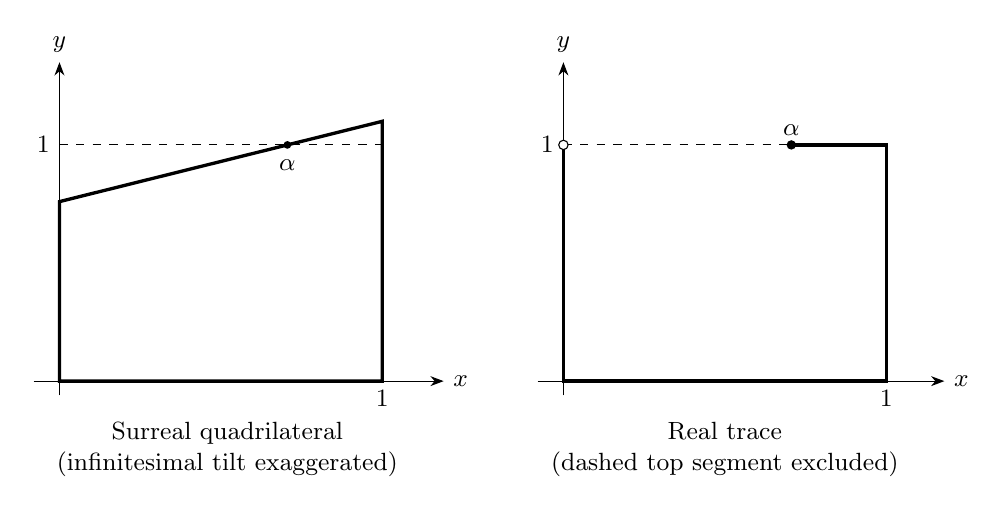
\begin{tikzpicture}[x=4.1cm,y=3.0cm,>=Stealth,font=\small]
 \begin{scope}
 \draw[->] (-.08,0)--(1.19,0) node[right]{$x$};
 \draw[->] (0,-.06)--(0,1.35) node[above]{$y$};
 \draw[dashed] (0,1)--(1,1);
 \draw[very thick] (0,0)--(1,0)--(1,1.10)--(0,.76)--cycle;
 \node[below] at (1,0){$1$};
 \node[left] at (0,1){$1$};
 \fill (.706,1) circle (1.4pt);
 \node[below] at (.706,.98){$\alpha$};
 \node[align=center] at (.52,-.29){Surreal quadrilateral\\(infinitesimal tilt exaggerated)};
 \end{scope}
 \begin{scope}[xshift=6.4cm]
 \draw[->] (-.08,0)--(1.18,0) node[right]{$x$};
 \draw[->] (0,-.06)--(0,1.35) node[above]{$y$};
 \draw[very thick] (0,1)--(0,0)--(1,0)--(1,1)--(.706,1);
 \draw[dashed] (0,1)--(.706,1);
 \draw[fill=white] (0,1) circle(1.7pt);
 \fill (.706,1) circle(1.7pt);
 \node[below] at (1,0){$1$};
 \node[left] at (0,1){$1$};
 \node[above] at (.706,1){$\alpha$};
 \node[align=center] at (.5,-.29){Real trace\\(dashed top segment excluded)};
 \end{scope}
\end{tikzpicture}
\caption{A four-vertex perturbation with a square shadow. The trace removes
$[0,\alpha)\times\{1\}$, including the upper-left corner, while retaining
the rest of the square. The left drawing is schematic, not a numerical
representation of an infinitesimal.}
\label{poly:ehr:fig:quad}
\end{figure}

\begin{corollary}[Algebraic input already suffices]\label{poly:ehr:cor:algebraic}
Taking $\alpha=1/\sqrt2$ gives the phenomenon over a real closure of
$\Q(\sqrt2)(\eps)$, with coefficients linear in one infinitesimal.
Thus neither real-algebraic flag coefficients, integral vertex shadows,
nor simplicity of the shadow guarantees a quasipolynomial counting function.
\end{corollary}

\begin{corollary}[Every dimension at least two]\label{poly:ehr:cor:dimensions}
For every $d\geq2$ there is a $d$-polytope with the labeled combinatorics
and integral vertex shadows of the unit $d$-cube whose counting series has
the unit circle as a natural boundary and whose sequence is not P-recursive.
\end{corollary}
\begin{proof}
Take $P_{\alpha,\eps}\times[0,1]^{d-2}$. Its counts are
\[
 (n+1)^{d-2}\bigl((n+1)^2-\lceil\alpha n\rceil\bigr).
\]
If these counts satisfied a polynomial-coefficient recurrence, substitution
would give one for $L_{P_{\alpha,\eps}}(n)$: replace each coefficient of
the shifted product by that coefficient times $(n+j+1)^{d-2}$. Nonzero
polynomial coefficients remain nonzero. This contradicts
Theorem~\ref{poly:ehr:thm:quad}. The series is therefore nonrational; its integer
coefficients have polynomial growth and radius $1$, so P\'olya--Carlson
applies again. Non-quasipolynomiality follows as well, since every
quasipolynomial sequence is P-recursive.
\end{proof}

\subsection{Why a sufficiently small real number is not a uniform substitute}

Replace $\eps$ in \eqref{poly:ehr:eq:quad} by a fixed small positive real $t$.
Ordinary Euclidean area is
\begin{equation}\label{poly:ehr:eq:area}
 \vol_2(P_{\alpha,t})
   =\int_0^1(1+t(x-\alpha))\,dx
   =1+t\left(\frac12-\alpha\right).
\end{equation}
The elementary lattice-cell estimate proved in Lemma~\ref{poly:ehr:lem:volume}
below gives
\[
 \lim_{n\to\infty}\frac{L_{P_{\alpha,t}}(n)}{n^2}
       =1+t\left(\frac12-\alpha\right)\ne1.
\]
In contrast the surreal count has leading coefficient $1$. Hence no fixed
positive real $t$ reproduces \emph{all} counting values. For each fixed
$n$, a sufficiently small $t$ does reproduce the value, as guaranteed by
Theorem~\ref{poly:ehr:thm:descent}.

For $\alpha=1/\sqrt2>1/2$ the discrepancy is especially explicit:
\[
 \lim_{n\to\infty}\frac{L_{P_{\alpha,t}}(n)-n^2}{n}=-\infty
                         \qquad(t>0\text{ fixed and small}),
\]
whereas taking the eventual $t\downarrow0$ value first yields
$2-1/\sqrt2$ after $n\to\infty$. The issue is the order of quantifiers,
not a numerical accuracy requirement.

\section{The universal surface coefficient}\label{poly:ehr:sec:surface}

We now describe what always survives from the first two Ehrhart
coefficients. The shadow in this section is a full-dimensional \emph{lattice}
polytope $Q\subseteq\R^d$, with $d\geq2$. A facet $F$ has direction
lattice
\[
 \Lambda_F=\operatorname{lin}(F-F)\cap\Z^d.
\]
Let $\mu_F$ be $(d-1)$-dimensional measure on $\aff F$, normalized so that
a fundamental parallelepiped of $\Lambda_F$ has measure one. Define
\begin{equation}\label{poly:ehr:eq:boundary-measure}
 A(Q)=\sum_{F\text{ facet of }Q}\mu_F(F).
\end{equation}
For the real trace $S$ of $P$, put
\begin{equation}\label{poly:ehr:eq:facet-piece}
 R_F=\cl_{\aff F}(S\cap\relint F).
\end{equation}
An empty or lower-dimensional $R_F$ has $\mu_F$-measure zero.

\subsection{The elementary counting estimates}

\begin{lemma}[Volume estimate for real polytopes]\label{poly:ehr:lem:volume}
For a full-dimensional bounded real polytope $T\subseteq\R^k$ and a
full-rank lattice $\Lambda$, with lattice-normalized measure $\mu$,
\[
 \#(nT\cap\Lambda)=\mu(T)n^k+O(n^{k-1}).
\]
The estimate also holds for a bounded convex semilinear set whose closure
is full-dimensional. A bounded subset of a fixed $j$-dimensional affine
space has at most $O(n^j)$ points of any fixed ambient integer lattice in
its $n$-dilate.
\end{lemma}
\begin{proof}
Choose a half-open fundamental parallelepiped of $\Lambda$. Its translates
tile the space and each contains exactly one lattice point under a fixed
consistent boundary convention. Associate such a tile with every lattice
point of $nT$. The symmetric difference between their union and $nT$ lies
in a neighborhood of the boundary of fixed width depending only on the
tile. A polytope has finitely many facets. The volume of that neighborhood
is $O(n^{k-1})$, by bounding a fixed-width neighborhood of each dilated
facet. Comparing the two volumes proves the first estimate. No rationality
of the vertices is used.

A bounded convex semilinear set has a closure that is a polytope: its finite
cell decomposition has finitely many closure vertices, and the convex
closure is their convex hull. The cells missing from the set but lying in
its closure have lower dimension, since a convex set contains the relative
interior of its closure. They contribute $O(n^{k-1})$ lattice points.
That bound, and the last assertion of the lemma, follow by placing disjoint
balls of fixed radius around the lattice points within the affine space
containing them. Distinct integer points have distance at least one, and
the dilated set lies in a ball of radius $O(n)$ in that space.
\end{proof}

\begin{lemma}[Classical interior coefficient]\label{poly:ehr:lem:interior-count}
For a full-dimensional lattice polytope $Q$ and $d\geq2$,
\begin{equation}\label{poly:ehr:eq:interior-count}
 \#(n\intr Q\cap\Z^d)
   =\vol_d(Q)n^d-\frac{A(Q)}2n^{d-1}+O(n^{d-2}).
\end{equation}
\end{lemma}
\begin{proof}
We use the classical Ehrhart polynomial and reciprocity
\cite{ehr:sam-woods}. Write $L_Q(n)=c_dn^d+c_{d-1}n^{d-1}+O(n^{d-2})$.
Lemma~\ref{poly:ehr:lem:volume} gives $c_d=\vol_d(Q)$, while reciprocity gives
$L_{\intr Q}(n)=(-1)^dL_Q(-n)$. Their difference, which counts the
boundary, has leading term $2c_{d-1}n^{d-1}$.

On the other hand the boundary is the union of its facets. Since every
facet contains a lattice vertex, its affine lattice on dilation is a
translate of $\Lambda_F$. Lemma~\ref{poly:ehr:lem:volume} gives its leading count
$\mu_F(F)n^{d-1}$. Intersections of facets have dimension at most $d-2$
and contribute $O(n^{d-2})$. Thus the boundary count has leading term
$A(Q)n^{d-1}$, proving $c_{d-1}=A(Q)/2$ and then
\eqref{poly:ehr:eq:interior-count}.
\end{proof}

\subsection{The coefficient formula}

\begin{theorem}[Boundary-trace surface coefficient]\label{poly:ehr:thm:surface}
Let $P\subseteq K^d$ be a real-bounded polytope whose shadow $Q$ is a
full-dimensional lattice polytope, with $d\geq2$. Then
\begin{equation}\label{poly:ehr:eq:surface}
 L_P(n)=\vol_d(Q)n^d+\beta(P)n^{d-1}+O(n^{d-2}),
\end{equation}
where
\begin{equation}\label{poly:ehr:eq:beta}
 \boxed{\displaystyle
 \beta(P)=\sum_F\left(\mu_F(R_F)-\frac12\mu_F(F)\right).}
\end{equation}
In particular
\begin{equation}\label{poly:ehr:eq:beta-bounds}
 -\frac{A(Q)}2\leq\beta(P)\leq\frac{A(Q)}2.
\end{equation}
\end{theorem}
\begin{proof}
By Lemma~\ref{poly:ehr:lem:interior}, every real interior point of $Q$ belongs to
the trace and no trace point lies outside $Q$. Decompose $S$ into its
interior part, its intersections with the relative interiors of the
facets, and its intersection with the union of the faces of codimension
at least two. The last part has $O(n^{d-2})$ lattice points after dilation,
by Lemma~\ref{poly:ehr:lem:volume}.

By Corollary~\ref{poly:ehr:cor:semilinear}, each
$S\cap\relint F$ is bounded, convex, and semilinear. Its closure $R_F$
is a real polytope, possibly empty or lower-dimensional. Choose a lattice
vertex $z_F\in F$. The lattice in $n\aff F$ is
\[
 \Z^d\cap n\aff F=nz_F+\Lambda_F.
\]
Translating by $nz_F$ and using the normalized measure, the preceding
lemma gives
\[
 \#\bigl(n(S\cap\relint F)\cap\Z^d\bigr)
   =\mu_F(R_F)n^{d-1}+O(n^{d-2}).
\]
If $R_F$ has smaller dimension, the same statement follows from the
packing bound with zero leading measure. Adding these finitely many
facet contributions to \eqref{poly:ehr:eq:interior-count} proves
\eqref{poly:ehr:eq:surface}--\eqref{poly:ehr:eq:beta}. Since $R_F\subseteq F$, each of its
measures lies between zero and $\mu_F(F)$, proving the bounds.
\end{proof}

\begin{example}[The quadrilateral revisited]
For the unit square, $A(Q)=4$. Three facets are retained up to sets of
one-dimensional measure zero; the retained portion of the top facet has
length $1-\alpha$. Therefore
\[
 \beta(P_{\alpha,\eps})=(4-\alpha)-2=2-\alpha,
\]
in agreement with \eqref{poly:ehr:eq:fractional}. The remaining term is the bounded
nonperiodic sequence $\{\alpha n\}$. Even in dimension two the $O(1)$
remainder need not approach a limit.
\end{example}

\begin{remark}[Why the shadow is assumed lattice]
If $Q$ is only rational, a dilated facet can meet the integer lattice on
some residue classes of $n$ and miss it on others. A single constant
surface coefficient need not exist even for $P=Q$. Theorem~\ref{poly:ehr:thm:surface}
is therefore not stated for arbitrary rational shadows. One can formulate
residue-class versions after tracking affine-lattice congruences, but
that additional bookkeeping is separate from the theorem proved here.
For any full-dimensional real shadow the simpler inclusions
$\intr Q\subseteq S\subseteq Q$ still give
$L_P(n)=\vol_d(Q)n^d+O(n^{d-1})$ by Lemma~\ref{poly:ehr:lem:volume}.
\end{remark}

\section{The full attainable interval, with fixed combinatorics}
\label{poly:ehr:sec:interval}

The bounds in \eqref{poly:ehr:eq:beta-bounds} are sharp not merely at their endpoints:
there are no gaps anywhere between them. More strongly, simplicity of the
shadow permits this freedom while preserving its entire labeled face lattice.

\begin{theorem}[Complete surface-coefficient range]\label{poly:ehr:thm:range}
Fix a full-dimensional lattice polytope $Q\subseteq\R^d$ with $d\geq2$.
Among real-bounded $K$-polytopes with shadow $Q$, the values of $\beta(P)$
are exactly
\[
 [-A(Q)/2,A(Q)/2].
\]
Every value can be attained using one positive infinitesimal and inequality
coefficients affine in that infinitesimal.
\end{theorem}
\begin{proof}
The upper and lower bounds were proved in Theorem~\ref{poly:ehr:thm:surface}.
Fix $0\leq\theta\leq1$. For each facet $F$, choose a point in its relative
interior and contract $F$ toward that point by the real factor
$\theta^{1/(d-1)}$. This gives a real polytope $T_F\subseteq F$ with
\[
 \mu_F(T_F)=\theta\mu_F(F).
\]
At $\theta=0$ it is a point. Choose affine functions $h_{Fj}$ cutting out
$T_F$ inside $F$, and let $s_F$ be the original nonnegative facet slack.
Define
\[
 P=\{x\in Q_K:s_F(x)+\eps h_{Fj}(x)\geq0
                         \text{ for all }F,j\}.
\]
Every real interior point of $Q$ belongs to $P$. Its shadow is $Q$ by the
same closed-shadow argument as in Theorem~\ref{poly:ehr:thm:implant}. For a real
point in $\relint F$, all other facet slacks are strictly positive, so only
the inequalities associated with $F$ matter. Its trace there is exactly
$T_F\cap\relint F$, whose closure has measure $\theta\mu_F(F)$.
Consequently
\[
 \beta(P)=(\theta-1/2)A(Q).
\]
As $\theta$ ranges through $[0,1]$, this gives the full claimed interval.
All rows are affine in the single parameter $\eps$.
\end{proof}

\subsection{Stability of a simple polytope under infinitesimal facet motion}

A $d$-polytope is simple if exactly $d$ facets meet at each vertex. Write
an irredundant facet representation of a fixed full-dimensional simple
real polytope as
\[
 Q=\{x\in\R^d:s_F(x)=b_F-a_F\cdot x\geq0\text{ for every facet }F\}.
\]
For arbitrary real affine forms $h_F=c_F+g_F\cdot x$, perturb only these
existing inequalities:
\begin{equation}\label{poly:ehr:eq:simple-perturb}
 P_\eps=\{x\in K^d:s_F(x)+\eps h_F(x)\geq0\text{ for all }F\}.
\end{equation}
Unlike \eqref{poly:ehr:eq:implant}, this construction is \emph{not} intersected
with $Q_K$.

\begin{lemma}[Simple labeled stability]\label{poly:ehr:lem:simple}
The polytope in \eqref{poly:ehr:eq:simple-perturb} is nonempty, full-dimensional,
and real-bounded. It has the same labeled face lattice as $Q$. Every
vertex has the standard part of its correspondingly labeled vertex in
$Q$, and its shadow is $Q$.
\end{lemma}
\begin{proof}
First we establish boundedness; this must precede taking standard parts
of hypothetical vertices. Since $Q$ is bounded, its recession cone
$\{u:a_F\cdot u\leq0\text{ for all }F\}$ is zero. Hence for every real
unit vector $u$,
\[
 f(u)=\max_F a_F\cdot u>0.
\]
By ordinary real compactness of the unit sphere, its minimum is a real
$c>0$. The first-order polynomial statement
\[
 \forall u\;\bigl(\sum u_j^2=1\ \Longrightarrow\
                         \bigvee_F a_F\cdot u\geq c\bigr)
\]
transfers to $K$. Choose real bounds for all the finitely many coefficients
of $g_F$. For unit $u\in K^d$, the error
$|\eps g_F\cdot u|$ is less than $c/2$, so some perturbed normal
$A_F=a_F-\eps g_F$ satisfies $A_F\cdot u\geq c/2$.
Choose a real $B>0$ exceeding every $|b_F+\eps c_F|$.
For nonzero feasible $x$, apply this to $u=x/\norm{x}$; a positive square
root exists because $K$ is real closed. Feasibility then gives
\[
 \frac c2\norm{x}\leq A_F\cdot x\leq b_F+\eps c_F<B.
\]
Thus $\norm{x}<2B/c$. The polyhedron is real-bounded. An ordinary interior
point of $Q$ has strictly positive real original slacks and therefore
strictly positive perturbed slacks, proving nonemptiness and full dimension.

Let $v$ be a vertex of $Q$, and $I(v)$ its $d$ incident facets. The
corresponding original normal matrix is nonsingular. The perturbed matrix
has the same nonzero determinant standard part, so its system has a unique
solution $v_\eps$ with $\st(v_\eps)=v$. At every other facet the original
slack at $v$ is strictly positive; hence its perturbed slack at $v_\eps$
is positive. The point $v_\eps$ is feasible and is a vertex, being the
intersection of $d$ independent active hyperplanes.

Conversely, a vertex $w$ of the perturbed full-dimensional polytope has
$d$ independent active rows. It is finite by the preceding bound. Taking
standard parts shows that $\st(w)\in Q$ lies on all of those $d$ distinct
original facets. In a simple polytope a point on $d$ distinct facets must
be a vertex: the facets through any positive-dimensional face are fewer
than $d$. One way to see this is to choose a vertex of that face; its
$d$ incident facet normals are independent, and the intersection of any
$d$ of them is that vertex alone. Thus these are exactly the incident
facets of an original vertex, and the corresponding original matrix is
nonsingular. Its unique perturbed solution is the already constructed
$v_\eps$. This proves that there are no other vertices.

At the constructed vertices the zero slacks are exactly the original zero
slacks. The vertex--facet table, and hence the labeled face lattice, is
unchanged. The vertex standard parts and Lemma~\ref{poly:ehr:lem:shadow} give the
shadow assertion.
\end{proof}

\begin{theorem}[Full range with fixed labeled simple combinatorics]
\label{poly:ehr:thm:simple-range}
Let $Q\subseteq\R^d$, $d\geq2$, be a full-dimensional simple lattice
polytope. Every
\[
 b\in[-A(Q)/2,A(Q)/2]
\]
is realized as $\beta(P)$ by a real-bounded $K$-polytope $P$ satisfying all
of the following simultaneously: its shadow is $Q$; its labeled face
lattice equals that of $Q$; its labeled vertex standard parts are exactly
the original integral vertices of $Q$; and it uses one affine-in-$\eps$
perturbation of each original facet inequality, with no added facets.
\end{theorem}
\begin{proof}
Put $\theta=1/2+b/A(Q)\in[0,1]$. For every facet $F$, choose a real affine
function $h_F$ for which
\begin{equation}\label{poly:ehr:eq:theta-cut}
 \mu_F(F\cap\{h_F\geq0\})=\theta\mu_F(F).
\end{equation}
Such a choice exists: a nonconstant linear functional on the
$(d-1)$-dimensional facet has sublevel sections whose volume varies
continuously from zero to full measure as the level traverses its range.
Continuity follows since the moving level hyperplane has measure zero
and the facet is bounded. For the endpoints use $h_F=-1$ or $h_F=1$.

Form $P_\eps$ as in \eqref{poly:ehr:eq:simple-perturb}. Lemma~\ref{poly:ehr:lem:simple}
proves all the geometric assertions. At a real point $x$ on
$\relint F$, exactly the original $F$-slack is zero; the others are
strictly positive. Consequently trace membership there is precisely
$h_F(x)\geq0$. The closure of that retained part has the measure in
\eqref{poly:ehr:eq:theta-cut}; deleting the boundary of $F$ does not change it.
Theorem~\ref{poly:ehr:thm:surface} therefore gives
\[
 \beta(P_\eps)=\sum_F(\theta-1/2)\mu_F(F)
             =(\theta-1/2)A(Q)=b.
\]
\end{proof}

Theorem~\ref{poly:ehr:thm:simple-range} says more than that one can choose open or
closed facets. Intermediate real portions of a facet, selected by an
infinitesimal tilt, continuously interpolate its contribution. Neither the
finite face lattice nor the full labeled list of vertex standard parts
records that selection. Simplicity is used only in the combinatorial
stability lemma; Theorem~\ref{poly:ehr:thm:range} establishes the interval without it.

\subsection{Dimension one behaves differently}

A real-bounded interval with a positive-length lattice shadow $[a,b]$, with
$a,b\in\Z$, retains all points of $(a,b)$ and independently retains or
excludes its two endpoints. Hence for $n\geq1$ its count is
\[
 (b-a)n-1+e_a+e_b,\qquad e_a,e_b\in\{0,1\}.
\]
Its constant term is one of $-1,0,1$, not an arbitrary value in an interval.
There is no positive-dimensional facet along which a threshold can slide.
This explains the $d\geq2$ condition in the continuous-range theorems.

\section{A rationality criterion that restores Ehrhart behavior}
\label{poly:ehr:sec:rational}

The preceding examples identify a failure of a natural extension of Ehrhart
theory. There is nevertheless a useful sufficient condition that replaces
rational vertex coordinates by rational data in the trace flags.

\begin{definition}\label{poly:ehr:def:rational-flags}
A real-bounded polytope has a \emph{rational flag presentation} if its real
trace is described by finitely many lexicographic nonnegativity conditions
on real affine forms all of whose coefficients are rational, together with
a rational bounding box. This is a property of a possible presentation,
not a claim about the canonicality of the basis in
Lemma~\ref{poly:ehr:lem:separated}.
\end{definition}

\begin{theorem}[Rational flags imply positive-dilation quasipolynomiality]
\label{poly:ehr:thm:rational-flags}
If $P$ has a rational flag presentation, then $L_P(n)$ is quasipolynomial
for positive integers $n$. Its ordinary generating function, with the
convention $L_P(0)=1$, is rational.
\end{theorem}
\begin{proof}
Use the hyperplane arrangement of the rational affine forms, including
the rational box boundary. The selected cells form a finite disjoint
union of relatively open rational polytopes $C_1,\ldots,C_s$. Each is the
relative interior of its closure, a rational polytope. For $n>0$ the
dilation map is injective and the dilated cells remain disjoint, so
\[
 L_P(n)=\sum_{j=1}^s\#(nC_j\cap\Z^d).
\]
Classical rational Ehrhart theory and reciprocity imply that the count of
the relative interior of a rational polytope is quasipolynomial on positive
integers \cite{ehr:sam-woods}. This statement includes lower-dimensional
rational affine hulls and their residue-class restrictions. A finite sum
of quasipolynomials is quasipolynomial, with period dividing a common
multiple of their periods. Splitting into residue classes shows that its
positive-index generating function is rational. Changing or supplying the
single coefficient at $n=0$ preserves rationality.
\end{proof}

\begin{example}[Why $n=0$ needs a convention]
Let $P=[\eps,1-\eps]$. Its trace is $(0,1)$, described by the rational
strict inequalities $x>0$ and $1-x>0$. Then
\[
 L_P(n)=n-1\quad(n\geq1),\qquad L_P(0)=1.
\]
The positive-dilation polynomial does not take the conventional value at
zero. Any theorem using relatively open trace cells must either treat
$n=0$ separately or adopt a different valuation convention there.
\end{example}

\begin{remark}[Not a necessary condition]
The theorem is a sufficient criterion, not an equivalence. Irrational
real polytopes can have polynomial counting functions; the examples of
Cristofaro-Gardiner, Li, and Stanley show that arithmetic cancellations
and period collapse must be taken seriously \cite{ehr:cgls}. Conversely, the
choice $\alpha=1/\sqrt2$ in Theorem~\ref{poly:ehr:thm:quad} shows that replacing
``rational'' by ``real algebraic'' in the hypothesis is insufficient.
An exact classification would have to detect cancellation among boundary
pieces rather than inspect each coefficient separately.
\end{remark}

\subsection{Three notions of rationality that must not be conflated}

A polytope may have rational or integral \emph{vertex shadows}; its trace
may admit a description by \emph{rational flags}; and its counting
\emph{generating function} may be rational. These are different properties.
The quadrilateral has integral vertex shadows but irrational trace data and
a nonrational generating function. Rational flags imply a rational
generating function by Theorem~\ref{poly:ehr:thm:rational-flags}. The manuscript
does not assert any converse from generating-function rationality to a
specific kind of geometric presentation.

The stronger descent theorem does not conflict with this distinction.
Its one-parameter algebraic coefficients can contain arbitrary real
constants. Eliminating extra infinitesimal scales is not the same as
eliminating irrational real thresholds.

\Needspace{16\baselineskip}
\subsection{A classical analytic dichotomy for every bounded trace count}

The analytic consequence of P\'olya--Carlson is more general than the
quadrilateral example. It supplies a useful complete dichotomy once the
geometric rationality question has been answered.

\begin{corollary}[Analytic classification of bounded counts]\label{poly:ehr:cor:dichotomy}
Let $P$ be any nonempty real-bounded finite $K$-polytope, without a
dimension assumption on its shadow, and let
$E_P(z)=\sum_{n\geq0}L_P(n)z^n$. The following are equivalent:
\begin{enumerate}[label=(\roman*)]
\item $E_P$ is rational;
\item $E_P$ is D-finite;
\item $L_P(n)$ is P-recursive;
\item $L_P(n)$ is eventually quasipolynomial.
\end{enumerate}
If these conditions fail, the unit circle is a natural boundary of $E_P$.
This is a direct application of classical results, not a new analytic
classification theorem.
\end{corollary}
\begin{proof}
A real bounding box gives $0\leq L_P(n)=O(n^d)$, and the values are integers.
If only finitely many are nonzero then $E_P$ is a polynomial. Otherwise
integrality and polynomial growth imply radius of convergence exactly one.
P\'olya--Carlson says that a nonrational such series has the unit circle as
a natural boundary \cite{ehr:bell-et-al,ehr:yu}. The finite-singularity argument
in Theorem~\ref{poly:ehr:thm:quad} then excludes D-finiteness. Conversely a rational
series is D-finite. The standard coefficient correspondence identifies
D-finiteness with P-recursiveness \cite{ehr:stanley-dfinite}.

In the rational case, the integer-coefficient form of P\'olya--Carlson
also says that every pole is a root of unity
\cite[Theorem 1.1]{ehr:bell-et-al}. Partial fractions therefore express the
coefficients, after a finite initial segment, as finite sums of terms
$n^j\zeta^n$ with $\zeta$ a root of unity. They are polynomial on residue
classes modulo a common order. Conversely, splitting an eventually
quasipolynomial sequence into its residue classes gives a rational series.
\end{proof}

\noindent[\wtag{} The root-of-unity clause is classically the
Fatou--Kronecker argument, not part of the natural-boundary dichotomy
proper. By Fatou's lemma a rational power series with integer coefficients
is $A(z)/C(z)$ with $A,C\in\Z[z]$ and $C(0)=1$. Radius of convergence~$1$
puts every root of the reversed polynomial, which is monic with integer
coefficients, in the closed unit disc. Kronecker's theorem then makes each
nonzero root a root of unity. Manuscript~03 cites this through the
integer-coefficient statement it attributes to
\cite[Theorem 1.1]{ehr:bell-et-al} and does not prove it; the equivalence of
(i) and (iv) rests on it.]

Thus for the present unweighted, one-variable counting problem there is
no intermediate nonrational D-finite case. The genuine remaining task is
to determine from the boundary geometry which side of the dichotomy occurs.

\section{Repository integration and the exact proof boundary}\label{poly:ehr:sec:repo}

\subsection{Snapshot and source use}

The repository tree inspected for this work had commit
\begin{center}
\texttt{6996fee43cc97b6c16351def7507d59a95bf62f0}.
\end{center}
The root and surreal-project readmes were consulted for orientation. The
surreal report guide and the omnific source below were then fetched at
this explicit commit. Code-search results may refer to older indexed
commits; they were used as locators, not as proof of the contents of the
pinned snapshot.

The key source is
\begin{quote}\small\ttfamily
Algebra/SurrealNumbers/Surreal/Foundations/\allowbreak OmnificUnits.lean
\end{quote}
Its namespace is \texttt{Surreal.Foundations.SignSequence}.
The three relevant declarations are
\begin{quote}\small\ttfamily
\begin{tabular}{l}
omnific\_eq\_intConstant\_of\_finite\\
omnific\_isFinite\_iff\\
omnific\_bounded\_iff
\end{tabular}
\end{quote}
The last states that an omnific integer has a real bound on its absolute
value exactly when it is an ordinary integer cast \cite{ehr:repo-units}.
This is the bridge in \eqref{poly:ehr:eq:finite-oz}.

The source was read; this work did \emph{not} rebuild the repository,
check its complete transitive axiom dependencies, or independently audit
its surreal-field implementation. The mathematical article can be read
independently using the standard normal-form argument given in
Section~\ref{poly:ehr:sec:setup}. None of its new trace, descent, implantation,
or surface-coefficient theorems is being represented as an existing
Lean theorem.

\subsection{A realistic formalization sequence}\label{poly:ehr:sec:lean-pointer}
\wtag{} The formalization roadmap of manuscript~03 is printed in
\cref{poly:sec:formalization}.

\subsection{A theorem dependency map}

\begin{center}
\small
\begin{tabular}{p{0.25\textwidth}p{0.39\textwidth}p{0.25\textwidth}}
\toprule
Result & Principal input & Status in this package\\
\midrule
Bounded omnific reduction & Normal form; repository boundedness theorem
 & Source inspected; direct mathematical argument\\[3pt]
Lexicographic trace & Standard part; finite real linear algebra
 & Full proof, no Lean certificate\\[3pt]
Algebraic descent & Trace expansion; real-closed transfer; curve selection
 & Full application proof with classical inputs\\[3pt]
Face implantation & Dominance of a real slack over an infinitesimal
 & Full constructive proof\\[3pt]
Surface coefficient & Trace cells; lattice-cell estimate; Ehrhart reciprocity
 & Full application proof\\[3pt]
Fixed-combinatorics range & Simple facet stability; continuous section volume
 & Full constructive proof\\[3pt]
Quadrilateral count & Exact lexicographic membership; finite row count
 & Full proof and exact finite checks\\[3pt]
Natural boundary & Nonrationality; P\'olya--Carlson
 & Classical analytic input explicitly used\\
\bottomrule
\end{tabular}
\end{center}

\section{Exact computational checks and reproducibility}\label{poly:ehr:sec:verification}

The accompanying \pathcode{code/03-boundary-geometry-verify.py} uses only the Python standard library.
All assertions use integers, rational numbers, exact arithmetic in
$\Q(\sqrt2)$, or polynomials in a formal positive infinitesimal ordered by
their first nonzero coefficient. No floating-point arithmetic is used to
resolve a boundary comparison.

\subsection{What was actually checked}

For $\alpha=1/\sqrt2$, the program verifies the 16 vertex--facet slacks of
the quadrilateral, its four positive cyclic orientation determinants, and
the exact shoelace identity
\[
 2\vol_2(P_{\alpha,\eps})=2+\eps(1-\sqrt2).
\]
It independently enumerates integer candidates in an enlarged bounding box
for every $1\leq n\leq150$: 1,205,575 candidate membership tests in total.
Every result agrees with \eqref{poly:ehr:eq:quad-count}. The ceiling formula and
its $0$--$1$ increments are checked for $1\leq n\leq10{,}000$.

For rational thresholds $\alpha=p/q$ with $2\leq q\leq12$ and
$1\leq p<q$, it checks 3,960 threshold/dilation cases, including vanishing
third forward differences on each tested progression of step $q$.
For the three-dimensional face implantation of
\[
 T=[1/\sqrt2,1]\times[1/\sqrt3,1]
\]
on the top of the unit cube, it checks all $1\leq n\leq35$ by 443,555
candidate tests against the exact formula
\[
 n(n+1)^2+
 \bigl(n+1-\lceil n/\sqrt2\rceil\bigr)
 \bigl(n+1-\lceil n/\sqrt3\rceil\bigr).
\]
Finally it verifies real specialization at
$t_n=1/(4(n+1))$ for $1\leq n\leq100$, using 353,700 exact
$\Q(\sqrt2)$ sign comparisons. The specialization parameter deliberately
depends on $n$.

For nonsquare positive integer $m$ and $n>0$, the program evaluates
\[
 \lceil n/\sqrt m\rceil=\operatorname{isqrt}(\floor{n^2/m})+1
\]
and verifies the defining inequalities
$m(c-1)^2<n^2<mc^2$. Thus the tests near the irrational cut do not depend
on a decimal approximation.

\begin{center}
\begin{tabular}{rrrr}
\toprule
$n$ & $\lceil n/\sqrt2\rceil$ & $L_{P_{1/\sqrt2,\eps}}(n)$ & $(n+1)^2$\\
\midrule
0&0&1&1\\
1&1&3&4\\
2&2&7&9\\
3&3&13&16\\
4&3&22&25\\
5&4&32&36\\
6&5&44&49\\
7&5&59&64\\
8&6&75&81\\
9&7&93&100\\
10&8&113&121\\
\bottomrule
\end{tabular}
\end{center}

The successful test report is in \pathcode{data/03-boundary-geometry-verification.json};
\pathcode{data/03-boundary-geometry-counts.csv} records values for $0\leq n\leq100$.
To reproduce the checks and compile the article, run
\begin{verbatim}
python3 code/03-boundary-geometry-verify.py --out-dir /path/to/scratch
latexmk -pdf -interaction=nonstopmode article.tex
\end{verbatim}
A double invocation of \texttt{pdflatex}, with an additional pass when
cross-references change, can replace \texttt{latexmk}. All figures are
contained in the TeX source; no external image assets are needed.

\noindent[\wtag{} Delivery names replaced. Manuscript~03 printed
\texttt{verify.py}, \texttt{verification.json}, \texttt{counts.csv} and
\texttt{python3 verify.py}; the shipped names are those above. Without
\texttt{--out-dir} the program writes \texttt{verification.json} and
\texttt{counts.csv} next to itself, that is, into \pathcode{code/}. The
report's recorded outputs are under \pathcode{data/} and should never be
overwritten, so pass an output directory outside the report. The program
writes the CSV with Python's \texttt{csv} module, so its lines end in CRLF
on every platform. The shipped
\pathcode{data/03-boundary-geometry-counts.csv} keeps those bytes: 102 lines
(a header and $n=0,\ldots,100$), each ending in CRLF, and marked
\texttt{-text} for Git. Manuscript~03's own TeX file
\texttt{surreal\_polytopes.tex} is not shipped: its text is this Part of the
report's \texttt{article.tex}, which the second command builds.]

\subsection{What finite checks do not establish}

Agreement through $10{,}000$ does not prove nonperiodicity or exclude a
large period. Those conclusions use the irrationality argument in
Theorem~\ref{poly:ehr:thm:quad}. The checks do not establish the general trace,
descent, or surface-coefficient theorems. They do not prove
P\'olya--Carlson, certify a natural boundary, or substitute for a proof
assistant. Their role is to catch arithmetic, incidence, dilation, and
endpoint mistakes in the explicit constructions.

\section{Further research questions}\label{poly:ehr:sec:questions}

The following are proposed research problems arising from this article.
Unless an external source is explicitly attached to a question, it is not
being represented as an established named open problem in the literature.

\begin{question}[An intrinsic classification of traces]\label{poly:ehr:q:intrinsic}
Which bounded convex semilinear sets $S\subseteq\R^d$ are the real traces
of finite polytopes over a real closed extension? Can one characterize them
without choosing a halfspace presentation over the extension?
\end{question}
Theorem~\ref{poly:ehr:thm:lex} provides a necessary finite lexicographic description.
Every finite conjunction of such descriptions has an infinitesimal
halfspace realization, but an arbitrary convex semilinear set is initially
given by a Boolean combination, not necessarily such a conjunction.
The useful target is a geometric characterization, including compatibility
of the selected portions on intersecting faces and a criterion for
prescribing the shadow when it loses dimension.

\begin{question}[Minimal trace depth and description size]
What is the least maximum lexicographic depth among all descriptions of a
fixed trace, and how does it trade off against the number of rows?
\end{question}
The $d+1$ bound proved here is a rowwise coefficient-space bound. It does
not prove that $d+1$ is an optimal invariant of traces after changing their
presentations. A normal form with canonical depth would be useful for
certificate design and for comparing independent constructions.

\begin{question}[Effective algebraic descent]
Given exact algebraic coefficients and a finite certificate for a
lexicographic presentation and incidence data, what degree, coefficient
height, and complexity bounds suffice for the descent curve in
Theorem~\ref{poly:ehr:thm:descent}?
\end{question}
Quantitative curve selection supplies relevant general machinery
\cite{ehr:basu-roy}. The open task here is to exploit the special multi-affine
ratio structure in \eqref{poly:ehr:eq:row-u}, account for the realization-space
quantifiers, and produce bounds suitable for an executable certificate.
The degree-$d$ trace-only compression is not already such a bound for
incidence-preserving descent.

\noindent[\wtag{} Related, not an answer: for coordinates given as
finite-support Hahn polynomials, Part~III's \cref{poly:mv:thm:compression}
(manuscript~06) specializes to ordinary Laurent polynomials in one parameter,
with an explicit integer grading and explicit sign thresholds. It keeps any
specified \emph{finite} certificate. Whether such a certificate can be
chosen to keep the whole real trace, and so give an effective descent with
degree bounds, is not proved in this report. Part~I's
\cref{poly:ts:thm:puiseux} is the non-effective real-algebraic analogue for
finite sign data.]

\noindent[\wtag{} \Cref{poly:part:cd} gives a lower-bound family for
rational arcs (\cref{poly:cd:thm:main}); no upper bound of the kind asked is
proved.]

\begin{question}[Surface freedom for nonsimple fixed combinatorics]
For a nonsimple lattice polytope $Q$, which values of $\beta$ can be
realized while preserving its labeled face lattice and all vertex shadows?
\end{question}
Theorem~\ref{poly:ehr:thm:range} gives the full interval when combinatorics is allowed
to change, and Theorem~\ref{poly:ehr:thm:simple-range} gives it with fixed
combinatorics when $Q$ is simple. At a nonsimple vertex, preserving several
dependent facet intersections imposes compatibility equations on the
perturbations. Determining whether these constraints shrink the interval,
and in which examples, is a sharply delimited next problem.

\begin{question}[The next asymptotic layer]
Which conditions ensure a coefficient of $n^{d-2}$, and can it be expressed
using traces on ridges and second-level facet data?
\end{question}
The surface term always exists for lattice shadows, but the bounded
fractional-part remainder in dimension two already prevents a universal
constant next term. A suitable theorem may require rational flags, averaging
in $n$, residue-class restrictions, or a discrepancy term rather than an
ordinary coefficient. Face implantation provides test cases with defects
localized at each codimension.

\begin{question}[Rationality and cancellation]
Within traces defined by real-algebraic flags, can one decide when the
counting series is rational, or characterize when irrational boundary
contributions cancel to give a quasipolynomial?
\end{question}
Rational flags give a sufficient condition; irrational period collapse
prevents a naive converse \cite{ehr:cgls}. The face-implantation identity reduces
many examples to lower-dimensional real-polytope enumeration, offering both
obstructions and constructive test families.

\begin{question}[Weighted and multivariate counting]
What replaces Corollary~\ref{poly:ehr:cor:dichotomy} for algebraic or real weights,
several dilation parameters, or generating functions recording individual
lattice coordinates?
\end{question}
The unweighted one-variable dichotomy is already resolved by that
corollary, including lower-dimensional shadows. Arbitrary real weights
remove the integer-coefficient hypothesis, while several variables require
an appropriate notion of boundary and multivariate D-finiteness. Existing
multivariate P\'olya--Carlson results provide relevant analytic input
\cite{ehr:yu}; the task is to identify geometric hypotheses that let these
results be applied to the proposed weighted or multivariate enumeration.

\begin{question}[Reciprocity with boundary data]
Is there a useful reciprocity formula for trace counts stated in terms of
constructible weights on faces rather than just open versus closed
polytopes?
\end{question}
A trace may retain a proper region of a facet and may make additional
choices on its boundary. Ordinary closed-polytope reciprocity cannot simply
be reused without recording those choices. The rational cell decomposition
in Theorem~\ref{poly:ehr:thm:rational-flags} provides a finite starting point, but
an intrinsic formula should be independent of the chosen subdivision.

\begin{question}[Symmetry-constrained perturbations]
What parts of the surface-coefficient interval remain attainable under
central symmetry or under a prescribed finite affine symmetry group?
\end{question}
The independent facet choices in Theorem~\ref{poly:ehr:thm:simple-range} need not
respect a group action. Averaging perturbations preserves some algebraic
symmetries but may change the selected boundary regions. Orbitwise
constraints and self-paired facets should be analyzed explicitly rather
than inferred from the unconstrained theorem.

\begin{question}[Finite enriched combinatorial invariants]
What finite augmentation of the face lattice and vertex shadows suffices
to reconstruct the real trace and its lattice counts?
\end{question}
The lexicographic affine flags are one sufficient description, but not an
intrinsic minimal invariant. Ordinary oriented-matroid signs alone forget
the real threshold data, while unrestricted valuation information is more
than the counting sequence needs. An invariant adapted to boundary flags
may bridge these extremes.

\begin{question}[Other integer parts and unbounded geometry]
How do the conclusions change for a different integer part of an ordered
field, or when coordinates and dilation parameters are allowed to be
infinite?
\end{question}
The present reduction depends on the exact bounded-element property
\eqref{poly:ehr:eq:finite-oz}. Infinite dilations do not automatically yield finite
sets of lattice points, so a new counting invariant must be specified
before an analogue of Ehrhart theory can be meaningfully formulated.
Ordinary cardinality, polynomial evaluation in an infinite argument, and
surreal-valued numerosity are not interchangeable definitions.

\noindent[\wtag{} \emph{Re-scoped: partly answered for hulls.} For integer
hulls rather than counts, \cref{poly:part:oih} treats arbitrary integer parts
(\cref{poly:oih:cor:integer-parts}) and infinite coordinates and right-hand
sides (\cref{poly:oih:thm:candidate,poly:oih:thm:descent}); the counting
half remains open.]

\begin{question}[A checked geometry pipeline]
Can the exact row-expansion, incidence, and finite-count certificates be
assembled into a Lean-checked pipeline with an explicitly small trust
boundary?
\end{question}
The immediate milestone is a checked proof of the quadrilateral count
and the bounded omnific reduction, followed by trace equivalence. A general
symbolic discovery procedure for arbitrary surreal inputs is a much
stronger demand and is not implied by the finite certificate theorems.

\section{Conclusion}

Finite surreal convex geometry has a classical combinatorial boundary:
its face lattices are already realizable over the real algebraic numbers.
Its arithmetic boundary is different. The real trace, not the standard-part
shadow, determines ordinary and bounded omnific lattice counts. That trace
is finitely lexicographic, and a single algebraic parameter can preserve
it together with the entire finite incidence structure.

Inside this finite framework, infinitesimal boundary motion is expressive.
It implants arbitrary lower-dimensional real-polytope counting functions,
changes the surface coefficient through its whole allowable interval, and
can do so without changing a simple lattice shadow or any of its labeled
vertex standard parts. A four-vertex, one-infinitesimal example already
escapes quasipolynomial and P-recursive enumeration. These statements give
a concrete research program and an exact formalization target without
requiring genuinely class-sized convexity or a new notion of infinite
lattice cardinality.

\section{Additional scope checks and potential failure modes (Appendix~A of manuscript~03)}\label{poly:ehr:app:scope}

\paragraph{Finite generators versus topological compactness.}
``Polytope'' means a finite convex hull, equivalently a bounded finite
halfspace system in the setting used here. Proofs over $K$ use linear
algebra or first-order transfer. The only compactness argument in the
simple-stability proof takes place on the \emph{real} unit sphere and is
then converted to a polynomial statement before transfer.

\paragraph{The interior-lifting hypothesis.}
A full-dimensional shadow ensures that its interior points belong to the
trace. It is not enough that $P$ itself have positive dimension, and even
full dimension of $P$ need not imply full dimension of its shadow. The
one-parameter descent theorem deliberately avoids relying on this lemma
and therefore allows rank loss in the shadow.

\paragraph{A representation-dependent flag is not an invariant.}
The separated basis exists for every finite coefficient space, but it is
not canonically chosen. The trace theorem asserts existence of a bounded-depth
presentation. It does not assert uniqueness of the scales or optimality
among all presentations.

\paragraph{Zero standard part does not mean zero slack.}
When a leading slack vanishes at a real point, its infinitesimal terms can
still decide membership. Dropping these terms is exactly the error exposed
by \eqref{poly:ehr:eq:quad-trace}. Conversely, a strictly positive real slack
cannot be overturned by a finite sum of infinitesimal corrections.

\paragraph{One parameter is not a uniform real approximation.}
An infinitesimal evaluation and a fixed positive real evaluation have
different quantifier meanings. Descent gives eventual agreement for each
fixed real point and each fixed finite lattice query. Equation~\eqref{poly:ehr:eq:area}
shows why a single real evaluation generally cannot answer all dilations.

\paragraph{Real-algebraic is not rational.}
All defining constants of the explicit quadrilateral can lie in
$\Q(\sqrt2)$, yet its count is not quasipolynomial. The rational flag theorem
requires rational coefficients for the real affine tests, not merely
algebraic coefficients or integral shadow vertices.

\paragraph{No general reciprocity theorem is smuggled in.}
Classical Ehrhart reciprocity is used for the lattice shadow in
Lemma~\ref{poly:ehr:lem:interior-count} and for rational cells in
Theorem~\ref{poly:ehr:thm:rational-flags}. It is not assumed for an arbitrary
irrational trace or for an arbitrary surreal polytope.

\paragraph{The analytic step has an external dependency.}
The arithmetic proof establishes nonrationality directly. The assertion of
a natural boundary uses P\'olya--Carlson, and the non-P-recursive conclusion
uses its analytic consequence together with the standard D-finite
correspondence. Finite experimental evidence is not used as a substitute
for any of these implications.

\section{Reproducibility and source ledger (Appendix~B of manuscript~03)}\label{poly:ehr:app:ledger}

The archive contains the TeX source, compiled PDF, standard-library
verification program, its JSON report, a CSV of example counts, and a
README. The bibliography gives stable DOIs or arXiv identifiers for the
classical inputs and commit-pinned paths for the two repository documents
used substantively. The source review was performed on September 30, 2026.
No repository files were modified or committed as part of this work.

\noindent[\wtag{} In this report the delivered verification program is
shipped as \pathcode{code/03-boundary-geometry-verify.py}, its JSON report as
\pathcode{data/03-boundary-geometry-verification.json}, and the CSV as
\pathcode{data/03-boundary-geometry-counts.csv} (CRLF line endings, as
delivered). The TeX source is printed as this Part, not shipped as a file.
The compiled PDF and the member README are not shipped; they survive only in
the delivery archive \pathcode{surreal_polytope_research.zip} of arrival
commit \pathcode{b2b626d85}.]

The source \texttt{OmnificUnits.lean} was returned with blob identifier
\begin{center}\small\ttfamily
c9ce3771e76d4b21ff76814682f37f63cc4664f8.
\end{center}
This identifies the inspected file; it is not a claim that the entire
repository was locally compiled. (\wtag{} The blob of this file at the
report's placement is still \texttt{c9ce3771}.) The article imports no unreviewed
research-report theorem as a hidden prerequisite: its surreal-specific
bounded-integer fact is also justified directly, and its remaining
external inputs are the classical mathematical results named in the text.


% ====================================================================
% Part V: Extension complexity beyond all orders
% Base: manuscript 07 (labels poly:ic:), member: manuscript 04 (labels poly:bao:)
% ====================================================================
\part{Extension complexity beyond all orders}\label{poly:part:ic}

\paragraph{Source and scope.}
\wtag{} This Part is built from two batch-58 manuscripts. Its base, printed
whole and in its own order, is manuscript~07, \emph{Invisible Complexity in
Surreal Polytopes}, subtitle \emph{Explicit polygons with identical all-order
jets and identical initial slack matrices}, author line ``Research manuscript
prepared for Vladimir Reshetnikov'', dated 30~September 2026 (archive
\path{surreal_polytopes.zip}, main file \path{surreal_polytopes.tex};
repository pin \texttt{6996fee43cc97b6c16351def7507d59a95bf62f0}; its
delivered PDF, which is not shipped, has 26 pages according to its README).
Into it are merged the results of manuscript~04, \emph{Beyond-All-Orders
Extension Complexity in Surreal Polygon Geometry}, subtitle \emph{Flat
deformations, classical face lattices, and a sharp-order complexity gap},
author line ``Research manuscript prepared for Vladimir Reshetnikov /
Developed with ChatGPT; independent review and formalization pending'', dated
September~30, 2026 (archive \path{surreal_polytopes_beyond_all_orders.zip},
main file \texttt{article.tex}; the same pin \texttt{6996fee43}; delivered PDF
of 26 pages, not shipped). The two manuscripts answer the same question:
explicit polygons whose coordinates agree to all orders of a chosen
infinitesimal with a polygon of small extension complexity, but whose own
extension complexity is much larger. Manuscript~07 is the base because it
covers every $n\geq4$ (04: $n=2^m$), linear \emph{and} semidefinite lifts,
residue descent for every convex valuation ring (04: standard part and
nonnegative rank only), every fixed dimension, and a sharper parameter count.
Manuscript~04 contributes a second construction on one circle with a
two-sided square-root order, a field- and scale-general classification of
when all-order jets lose information, a finite-order rank-one analogue,
failure of lifting coherent finite-order factorizations, algebraic
finite-accuracy approximants, a rational-chart generalization and an
in-principle decision procedure. Every item of 04 is printed where it
belongs and marked ``source~04''; items proved by both manuscripts are
printed once and name both. Labels of 07 carry the prefix
\texttt{poly:ic:}, labels of 04 the prefix \texttt{poly:bao:}. This Part
keeps its own definitions and hypotheses: the finite-element ring $\OO$,
standard part $\st$ and convex hulls are those of \cref{poly:part:lift}, restated here in the words of 07 and 04. The
formalization roadmap of 07 is printed in \cref{poly:sec:formalization};
nothing in this Part is formalized.

\paragraph{Notation in this Part.}
\wtag{} The valuation is written $\nu$ throughout this Part, with the
convention of 04: $\nu(x)>\nu(y)$ precisely when $x/y$ is infinitesimal, so
a \emph{larger} value means a \emph{smaller} element and
$\nu(\omega^{-\gamma})=\gamma$. (Manuscript~07 writes $\nu$ without defining
it; manuscript~04 writes $\vv$; we renamed 04's $\vv$ to $\nu$. Manuscript~04
also uses $\nu_i$ for monomials in the proof of
\cref{poly:bao:thm:rankone}; those are renamed $\mu'_i$.) The natural value
group is $G$ (07's letter; 04's $\Gamma$ in its Section~3 is renamed $G$);
$\Gamma$, $\Gamma_2$ and $\Gamma_n$ denote the specific groups
\eqref{poly:ic:eq:gamma}, \cref{poly:ic:cor:ranktwo} and
\eqref{poly:bao:eq:ranktwo}. The flat ideal of a positive infinitesimal
scale $x$ is written with one symbol, $\JJ_x=\bigcap_{m\geq1}x^m\OO$
(07's $\mathfrak j$); manuscript~04's $\mathcal I_\eps$ is printed as
$\JJ_\eps$. The jet scale is always the subscript of $\JJ$: a general
positive infinitesimal is $s$ in statements from 07 and $\eps$ in
statements from 04 (\cref{poly:bao:sec:flat,poly:bao:thm:criterion,poly:bao:thm:chart});
in 04's explicit family it is specialized to $\eps=\omega^{-1}$, the
report's $\eps$. Manuscript~07's main construction uses the fixed scale
$\rho=\omega^{-\omega}$; following the report-wide convention it is printed
as $\tau=\omega^{-\omega}$ wherever it denotes that surreal. Where 07
re-chooses the scale, the letter $\rho$ is kept as a general parameter: in
\cref{poly:ic:cor:ranktwo} ($\rho=\omega^{-1}$) and in
\cref{poly:ic:thm:precision} (a chosen infinitesimal); the auxiliary bound
called $\tau$ in the proof of \cref{poly:ic:thm:precision} is renamed
$\sigma$, and the tolerance set $\mathcal T\ni\tau$ of 04's
\cref{poly:bao:thm:tolerances} is renamed $\mathcal D\ni\delta$ (07's
letters). The two quoted abstracts keep their own letters: $\rho$ in 07's
abstract is this Part's $\tau$, and $P_n$ in 04's abstract is this Part's
$P^\circ_n$. Tempting false readings, with the true one beside them:
\begin{itemize}
\item $P_n,Q_n$ (07) are polygons in the triangle $T$; manuscript~04's
cyclic polygon on the unit circle, also called $P_n$ there, is printed as
$P^\circ_n$ with vertices $p^\circ_i$, and its regular reference polygon is
$R_n$ with vertices $r_i$. $R_N$ in \eqref{poly:ic:eq:reflection} is 07's
reflection map, not a polygon.
\item $\st$ is the standard part. $\OO/\JJ_s$ is a different quotient and
is not $\R$; the coarse residue field of $V_\tau$ (\cref{poly:ic:prop:coarsering})
is a third one. Manuscript~04's ``algebraic finite-accuracy shadows'' are
real-algebraic approximants, not standard parts; we call them
\emph{approximants} (\cref{poly:bao:cor:algshadow}).
\item $\tr$ is the matrix trace (07), not Part~IV's real trace $\Tr$.
\item $q_i$ are 07's easy vertices; in 04's text $q_i$ are distinct ordinary
primes, entering only through $\sqrt{q_i}$ and $\mu_i=\omega^{-\omega\sqrt{q_i}}$.
$a_n$ (07) is the real root of $X^{2n+1}-2$; $a_i$ (04) is $\tan(\theta_i/2)$.
\item $\eta_\ell$ (07) are perturbation monomials and $\eta=\eta_1$; in 04,
$\eta$ is a flat bound (\cref{poly:bao:prop:observations}) or a positive
rational tolerance (\cref{poly:bao:cor:algshadow}).
\item $D$: 07's orientation determinant $D(X,Y,Z)$ of points and
$D=h(h+1)/2$ in \cref{poly:ic:thm:genericpsd}; 04's $D(a,b,c)$ is the
orientation determinant in circle parameters \eqref{poly:bao:eq:orientation}.
$H_N$ (07) is a parabola hull; $H(V)$ (04) is a $3\times n$ point matrix.
\item $m$: an ordinary integer exponent in 07 ($\JJ_s$, $\powprec$) and in
04 $n=2^m$; $M$ is 04's exponent letter. $\mm$ is the maximal ideal of
$\OO$. $T$ is 07's triangle, but also a nonnegative factor matrix in 04
($S=TU$) and in the proof of \cref{poly:ic:thm:shadowdescent}; $U(n)$ is
07's easy bound, $U$ also a factor matrix. $S$ is always a slack matrix.
\item $K$ is a set-sized real closed field; $K_0$, $K_n$ and $F_n$ are
specific fields of 07 and 04; $k$ is a residue field in
\cref{poly:ic:sec:residue} and $k=n-2$ in 07's construction.
\end{itemize}
Across the report: $\rho$ here is not Part~III's threshold $\rho_g$ nor
Part~IV's separated scales $\rho_1\gg\dots\gg\rho_r$; $V_\tau$ is not Part~I's
dependence space nor Part~III's mixed volume.

\paragraph{Abstract of manuscript 07.}
Can the real shadow, the complete expansion at a chosen infinitesimal scale,
or the leading terms of a slack matrix determine the exact complexity of a
surreal polytope? We give explicit negative answers for both linear and
positive-semidefinite lifts. For every ordinary finite $n\geq4$ we construct
two strictly convex, labeled surreal $n$-gons $Q_n,P_n$ inside the same real
triangle. They have the same real shadow and oriented matroid; their vertex
coordinates and canonical slack matrices agree modulo every power of a
specified infinitesimal $\rho$; and corresponding nonzero slack entries have
identical valuations and leading coefficients. Nevertheless,
\[
 \xc(Q_n)\leq 2\lceil\log_2(n-2)\rceil+2,
 \qquad \xc(P_n)\bigl(\xc(P_n)-1\bigr)\geq 2n,
\]
and $\sx(P_n)\geq(2n)^{1/4}$, while $\sx(Q_n)\leq\xc(Q_n)$.
Every coordinate is a sum of at most three Conway monomials, and all examples
fit one set-sized real closed subfield of valuation rank three.

The proof combines a binary reflection lift with explicit algebraically
independent, beyond-all-powers perturbations. We supply a non-Archimedean
proof of the generic semidefinite lower bound using finite definability,
rather than rational exposing objectives, which can fail over the surreals.
We also prove residue descent for nonnegative and semidefinite ranks,
identify the exact kernel of power-jet observations, establish a sharp
rank-one/rank-two boundary for all-order ambiguity, and extend the construction
to arbitrary set-sized precision requirements.

These are proved statements within the manuscript, not a claim to have
settled a previously named classical conjecture. The generic lower bounds,
reflection method, cone-factorization correspondence and real-closed-field
transfer are classical. The proposed contribution is their explicit
multiscale separation package. Priority and correctness have not been
independently certified; no Lean formalization is claimed.

{\small\color{ink}Keywords (manuscript 07): surreal polytope; extension complexity; nonnegative rank;
semidefinite rank; convex valuation ring; infinitesimal perturbation;
real closed field; formal jets.\par}

\paragraph{Abstract of manuscript 04.}
Infinitesimal coordinates do not create new finite polytopal face lattices:
real-closed-field transfer already prevents this. They can, however, conceal
large changes in extension complexity beneath every power of a prescribed
infinitesimal. We construct explicit cyclic surreal $n$-gons $P_n$, for
$n=2^m$, and regular $n$-gons $R_n$ on the same unit circle such that their
labeled vertex coordinates agree modulo $\varepsilon^M\OO$ for every ordinary
integer $M\geq1$, where $\varepsilon=\omega^{-1}$. Nevertheless,
\[
 m\leq\xc(R_n)\leq2m,
 \qquad
 \lceil\sqrt n\rceil\leq\xc(P_n)\leq\min\{n,\lceil24\sqrt n\rceil\}.
\]
The polygons also have identical standard parts, leading affine Pl\"ucker
data, and leading slack matrices; every finite linear objective has an
optimal-value difference smaller than every power of $\varepsilon$.
The construction uses algebraically independent Conway monomials and a
rational parametrization of the circle. A general theorem identifies the
exact boundary: over any real closed $K\supseteq\R$, unbounded such gaps in
all-order jet fibers occur precisely when
$\bigcap_{M\geq1}\varepsilon^M\OO\neq0$, equivalently when
$\nu(\varepsilon)$ is not an order unit of the natural value group.
We give full proofs of these statements, a finite-order rank-one analogue,
a rational-chart generalization, and an explicit account of why finite
real-algebraic transfer is compatible with the obstruction. The classical
extension-complexity bounds are credited separately from the proposed
flat-geometric synthesis.

\paragraph{Status (manuscript 04).}
This is a research manuscript, not a claim of a
refereed breakthrough or a Lean-checked result. The flat-fiber theorems and
explicit all-order examples are offered as proposed contributions. Their
priority has not been independently certified. No named published conjecture
is claimed solved. The auxiliary exact checks verify identities and finite
examples, not the asymptotic lower bounds.

\medskip\noindent
\wtag{} Manuscript~07 has no separate status paragraph; its status is the
last paragraph of its abstract above and its table in
\cref{poly:ic:sec:scope}. In 04's abstract the valuation symbol is printed
as $\nu$ (04: $\vv$).

\section{The questions, the answer, and the research boundary}\label{poly:ic:sec:scope}

A polytope can be geometrically almost indistinguishable from another and
still require a much larger exact optimization model. Surreal coefficients
make it possible to ask a stronger version: can the difference remain
invisible not merely at a small numerical tolerance, but at \emph{every}
power of a prescribed infinitesimal? The answer is yes, even with the same
number of vertices, the same full-dimensional real shadow and the same
leading slack data.

Here a linear extended formulation is an exact description of a polytope
as an affine image of a polytope in a possibly larger space. Its size is the
number of facet inequalities; equations do not count. A semidefinite lift
uses an affine slice of the cone of positive-semidefinite symmetric
matrices. Its size is the matrix order, not the number of scalar entries.
Both notions are exact and allow arbitrary coefficients in the ambient
real closed field.

The concrete questions answered below are the following.
\begin{enumerate}[label=\textbf{(\arabic*)},leftmargin=*,itemsep=3pt]
\item Does equality of all power jets of labeled vertices force comparable
linear or semidefinite extension complexity? No: the ratios are unbounded.
\item Does the zero pattern together with every leading valuation and
leading coefficient of a slack matrix determine these complexities? No,
even for rank-three slack matrices of polygons.
\item Does taking a real or more general ordered residue lose complexity
in a controlled direction? Yes: both complexities can only decrease.
\item Is non-Archimedean order alone sufficient for nontrivial all-order
ambiguity? No: the chosen scale must fail to be an order unit in the value
group. Valuation rank two is necessary and sufficient for examples with
one layer of such ambiguity.
\end{enumerate}
These are questions formulated and answered here. They are not presented
as a list of previously published open conjectures.

\subsection{The question of manuscript 04}\label{poly:bao:sec:intro}
\wtag{} The following is the opening of manuscript~04 (its Section~1, ``The
question and the main result''); its explicit family and main theorem are
printed in \cref{poly:bao:sec:construction}.

A polytope can be complicated in two different ways. Its vertices and faces
can have an intricate incidence pattern, or its particular coordinates can
make it difficult to express as the projection of a simpler polytope. The
first notion is combinatorial. The second is measured by
\emph{extension complexity}: the minimum number of facets of a
higher-dimensional polytope that projects onto the given one.

For a polygon, every face lattice is a cycle. This leaves considerable room
for coordinate-dependent behavior. Regular polygons have logarithmic
extension complexity, whereas suitable generic polygons require at least
square-root complexity. These are classical facts, not discoveries of this
manuscript \cite{ic:frt,ic:kp}. Kwan, Sauermann, and Zhao proved that every
\emph{cyclic} $n$-gon---one with all vertices on a circle---has extension
complexity at most $24\sqrt n$ \cite{bao:KSZ}. Here ``cyclic polygon'' does not
refer to the higher-dimensional cyclic polytopes on the moment curve.

The question investigated here is more refined:
\begin{quote}
Can a polygon be indistinguishable from a regular polygon at every order
of a fixed infinitesimal scale, while retaining square-root rather than
logarithmic extension complexity?
\end{quote}
The answer is affirmative in the surreal field, and its exact valuation
theoretic boundary can be identified. The interesting phenomenon is not a
new abstract face lattice. It is loss of information about an exact
existential problem under an all-order asymptotic observation map.

\wtag{} Question~(1) of 07 and the question of 04 are the same question for
two reference polygons: a logarithmic-size polygon in a triangle (07) and a
regular polygon on the unit circle (04). Question~(4) of 07 and 04's
``exact valuation theoretic boundary'' are the same order-unit theorem
(\cref{poly:ic:thm:orderunit}, with its two-sided consequences
\cref{poly:ic:cor:ranktwo} and \cref{poly:bao:thm:criterion}).

\subsection{Relationship to ProveIt and the previous convexity report}
The selected repository documentation describes a surreal field development,
real closedness, surcomplex algebraic closedness, finite geometry, and a
large collection of research reports. It explicitly separates research
claims from statements mapped to Lean declarations \cite{ic:repo,ic:surrealrepo}.
The repository snapshot recorded during this investigation is
\texttt{6996fee43cc97b6c16351def7507d59a95bf62f0}, dated 30 September 2026.
The audit consulted the root README, the surreal README, the report catalogue,
and selected directory metadata; it was not an exhaustive theorem-by-theorem
audit or an independent rebuild.

\noindent[\textup{[write]} The draft corrected here, \emph{Finite Convexity and Exact Lexicographic Optimization over the Surreals} (22~September 2026), was supplied privately to the authors of manuscripts 05 and 07; it is not part of ProveIt and could not be checked. The statements below are printed as standalone results.]

The earlier draft \emph{Finite Convexity and Exact Lexicographic Optimization
over the Surreals} already treats finite Farkas theory, linear-programming
duality, finite convexity theorems and exact lexicographic compilation
\cite{ic:previous}. That draft was located in the supplied research library;
its presence in the maintained repository tree was not established in this
audit. The present paper does not reclassify that material as new. Instead,
it studies \emph{the size of exact lifts and the information lost by scale
reduction}.

\subsection{Relation to ProveIt (source 04)}
The inspected snapshot of \texttt{VladimirReshetnikov/ProveIt} contains a
surreal-number library and a collection of research reports that explicitly
distinguish manuscript arguments, finite computational tests, and mapped
Lean declarations \cite{bao:Repo,bao:RepoGuide}. Its computer-algebra report also
separates exact denotation from approximation and from decidable equality
\cite{bao:RepoCAS}. The present work develops a geometric consequence of that
separation: even complete information at every power of one selected scale
need not determine a finite exact optimization invariant.

We use the established ordered-field and normal-form foundations. We do not
assume the correctness of the repository's unreviewed new research claims.
The source snapshot and the limited inspection scope are recorded in
\cref{poly:bao:sec:audit}. The current paper supplies no Lean development and makes
no assertion about having rebuilt the repository.

\wtag{} Both descriptions were re-checked against the current tree. The
surreal README (\path{Algebra/SurrealNumbers/README.md}, lines 1--27
and 147) describes the report collection, the real closed surreal field,
the algebraically closed surcomplex numbers, finite geometry among the
formalized topics, and the ledger that maps statements to Lean
declarations; the computer-algebra report's README
(\path{Algebra/SurrealNumbers/docs/foundations-and-computation/computer-algebra/README.md},
lines 24--28) separates ``exact denotation from effective coefficient
access from decidable equality/order from certified approximation''. The
Lean module \path{Surreal.Surcomplex.RegularPolygon}
(\path{Algebra/SurrealNumbers/Surreal/Surcomplex/RegularPolygon.lean}:
\texttt{vertex}, \texttt{vertex\_radius}, \texttt{side\_length},
\texttt{area\_eq}) formalizes regular polygons at surreal radius, which is
related to 04's regular $R_n$, but neither manuscript uses it; nothing in
this Part is formalized.

\subsection{What is classical and what is proposed here}
Fiorini, Rothvo\ss{} and Tiwary established generic polygon lower bounds and
small extended formulations for special polygons \cite{ic:frt}. Reflection
relations are an established tool for compact formulations \cite{ic:kp}.
Gouveia, Robinson and Thomas proved the generic semidefinite lower bound
\cite{ic:grt}. The slack-factorization interpretation originates with
Yannakakis and its cone generalization \cite{ic:yannakakis,ic:gpt}; normalization
and lower-semicontinuity methods for positive ranks are also established
\cite{ic:psdrank}.

\begin{center}
\begin{tabular}{@{}p{.31\textwidth}p{.62\textwidth}@{}}
\toprule
Component & Status in this manuscript \\
\midrule
Generic rank bounds & Classical mechanism, reproved over arbitrary real
closed fields; the semidefinite proof avoids an Archimedean step.\\
Binary reflection lift & Explicit specialization of the classical
reflection-relation method.\\
Residue descent & Valuation-ring formulation with algebraic proofs;
not claimed as a new closure theorem.\\
Explicit $P_n,Q_n$ & Proposed separation package: finite monomial support,
all-order agreement, identical initial slacks, and diverging lift sizes.\\
Rank and precision boundary & Consequences proved here, with the exact
scale and set-size hypotheses stated.\\
Formal verification & Finite exact computational checks only; no
machine-checked proof of the manuscript.\\
\bottomrule
\end{tabular}
\end{center}

Searches of the selected documentation and primary literature did not locate
this exact explicit separation package. This is a limited novelty check,
not evidence that every related formulation is absent from the literature.
All uses of ``new'' should therefore be understood as \emph{candidate new
formulations and consequences}, subject to expert review.

\subsection{What is new here, and what is imported (source 04)}
The proposed contribution is the combination of exact circular geometry,
explicit nonreal algebraic independence, and agreement to \emph{all}
orders, together with a necessary-and-sufficient condition for the same
phenomenon in arbitrary real closed extensions of $\R$. The resulting
failure of reconstruction persists even after one supplies all leading
Pl\"ucker coordinates, all leading slack entries, and every finite-direction
linear optimization value to all orders.

The following ingredients are established mathematics: real closedness of
the surreal field and uniqueness of Conway normal forms \cite{bao:vDE};
quantifier elimination for real closed fields \cite{bao:Tarski,bao:Collins};
Yannakakis' slack-factorization theorem \cite{ic:yannakakis}; reflection
constructions for regular polygons \cite{ic:kp}; and the polygon bounds just
cited. We prove the needed elementary extensions and calculations rather
than treating the phrase ``by transfer'' as a substitute for specifying the
finite formula.

\section{Fields, polytopes, lifts, and power-jet information}\label{poly:ic:sec:setup}

\subsection{Set-sized fields first}
Unless otherwise stated, $K$ is a set-sized real closed ordered field.
For standard parts we assume $K\supseteq\R$. A finite surreal configuration,
and any finite collection of putative lift certificates, lie in a set-sized
real closed subfield of $\No$: generate an ordered field from their
coefficients and take its relative real closure in $\No$. Thus every
first-order argument below is made in a genuine set-sized field.

We use the classical real closedness and normal-form arithmetic of $\No$
\cite{ic:gonshor}. In particular,
\begin{equation}\label{poly:ic:eq:monomials}
 \omega^a\omega^b=\omega^{a+b},
 \qquad a<b\Longrightarrow \omega^a\ll\omega^b,
\end{equation}
where $x\ll y$ means $|x|<y/m$ for every positive ordinary integer $m$.
A nonzero finite sum of distinct Conway monomials cannot vanish. All
arithmetic inside an exponent is surreal \emph{field} arithmetic; no
unstated ordinal-arithmetic convention is used.

Every $n,m,r,k$ in this paper is an ordinary finite integer. No result
concerns a polytope with an infinite number of vertices. A statement about
lifts ``over $\No$'' means a statement about finite coefficient certificates;
it does not apply first-order model theory directly to a proper class.

\subsection{Finite convexity and the two lift sizes}
For $v_1,\ldots,v_N\in K^d$ define
\[
 \conv_K(v_1,\ldots,v_N)=
 \left\{\sum_j\lambda_jv_j:\lambda_j\geq0,
                         \ \sum_j\lambda_j=1\right\}.
\]
Dimension and facets are relative to the affine hull. A vertex is an extreme
point. The finite vertex--facet correspondence, linear-programming duality
and the finite Farkas alternative hold over real closed fields. They follow
from their finite algebraic proofs or from real-closed-field transfer.
No order-topological compactness is assumed.

We allow size zero for a point (a constant affine image of the zero-dimensional cone).
For a positive-dimensional polytope $P$, let $\xc_K(P)$ be the smallest
number of facets of a polytope $E$ admitting an affine surjection onto $P$.
The usual definition allowing polyhedral extensions gives the same number.
Indeed, a nonnegative factorization of a slack matrix gives a bounded
extension after zero factor columns are removed: each remaining
nonnegative auxiliary coordinate is bounded by a bounded slack divided by
a fixed positive entry. This also explains why unbounded lifts cannot
circumvent the lower bound proved later.

Let $\Sym^k(K)$ denote the symmetric $k\times k$ matrices. Write
$\Sym^k_+(K)$ for the positive-semidefinite cone; equivalently, every
principal minor is nonnegative. Define $\sx_K(P)$ as the least $k$ for
which an affine slice of $\Sym^k_+(K)$ has an affine image equal to $P$.
The slice itself need not be bounded.

\begin{definition}[Two factorization ranks]\label{poly:ic:def:ranks}
For a nonnegative matrix $M\in K^{f\times N}$, $\rankp^K(M)$ is the least
$r$ such that $M=UV$ with $U\in K_{\geq0}^{f\times r}$ and
$V\in K_{\geq0}^{r\times N}$. Its semidefinite rank $\rankpsd^K(M)$ is the
least $k$ admitting $A_i,B_j\in\Sym^k_+(K)$ with
$M_{ij}=\tr(A_iB_j)$.
\end{definition}

A facet--vertex slack matrix of $P=\{x:Ax\leq b\}=\conv(v_j)$ has entries
$S_{ij}=b_i-A_i v_j$. The classical factorization theorems imply
\begin{equation}\label{poly:ic:eq:factorization}
 \xc_K(P)=\rankp^K(S),\qquad
 \sx_K(P)=\rankpsd^K(S),\qquad
 \sx_K(P)\leq\xc_K(P).
\end{equation}
We import the real factorization theorem \cite{ic:yannakakis,ic:gpt}. Its
extension to $K$ needs no analytic limiting argument: for each fixed
finite dimension, vertex count, facet count and proposed rank, existence
of a factorization and existence of a lift are first-order statements in
ordered-field arithmetic. Positive semidefiniteness is a finite list of
principal-minor inequalities. The universal equivalence over $\R$
therefore holds over every real closed field. Quantifier elimination for
these fields is the standard algebraic input; see also its formalized
constructive treatment in \cite{ic:cohenmahboubi}.

\wtag{} Manuscript~04 proves the linear half of
\eqref{poly:ic:eq:factorization} directly over $K$, checking the field and
boundedness issues instead of transferring; it is printed as
\cref{poly:bao:prop:yann} in \cref{poly:bao:sec:xc} below.

\subsection{Finite elements, standard part, and all power jets}
Suppose now that $K\supseteq\R$. Its finite-element ring and infinitesimal
ideal are
\[
 \OO=\{x\in K:|x|\leq c\text{ for some }c\in\R_{>0}\},\qquad
 \mm=\{x:|x|<1/m\text{ for every }m\geq1\}.
\]
Completeness of the \emph{ordinary real coefficient field} identifies
$\OO/\mm$ with $\R$; write the residue map as $\st$. This does not assert
completeness of $K$.

For a positive infinitesimal $s$, define
\begin{equation}\label{poly:ic:eq:flatideal}
 \JJ_s=\bigcap_{m\geq1}s^m\OO.
\end{equation}
Equality of all $s$-power jets means equality in every quotient
$\OO/s^m\OO$, or equivalently that the difference lies in $\JJ_s$.
For a vector, $\JJ_s^M$ denotes the Cartesian power of the ideal.
These are quotients of the \emph{valuation ring}, not of the field $K$.
In a field the ideal generated by a nonzero $s$ is the whole field.

\wtag{} Manuscript~04 (its Section~3) fixes a positive infinitesimal
$\eps\in K$ and sets
\begin{equation}\label{poly:bao:eq:flatideal}
 \JJ_\eps=\bigcap_{M\geq1}\eps^M\OO,
\end{equation}
the same ideal for $s=\eps$ (04 writes $\mathcal I_\eps$). Here and
throughout 04's text $M$ ranges over ordinary finite integers.

For positive infinitesimals $a,b$ we write
\[
 a\powprec b\quad\Longleftrightarrow\quad
              0<a<b^m\quad\hbox{for every }m\geq1.
\]
This notation means ``smaller than every power,'' not merely $a<b$.

\begin{lemma}[The power-flat ideal; sources 07 and 04]\label{poly:ic:lem:flat}\label{poly:bao:lem:flat}
For every positive infinitesimal $s$,
\[
 \JJ_s=\{x\in K:|x|<s^m\text{ for every }m\geq1\}.
\]
It is a prime ideal of $\OO$ and the kernel of
\[
 \OO\longrightarrow\varprojlim_m\OO/s^m\OO.
\]
Moreover $s^{-h}\JJ_s=\JJ_s$ for each integer $h\geq0$.
\srcnote{source 04} For $x\in\OO$, membership $x\in\JJ_s$ is also
equivalent to $\nu(x)>M\nu(s)$ for every $M\geq1$, with $\nu(0)=+\infty$;
and $\JJ_s$ is a \emph{convex} prime ideal of $\OO$.
\end{lemma}
\begin{proof}
If $x\in s^{m+1}\OO$, write $x=s^{m+1}u$ with $u$ finite. Then
$|su|<1$, so $|x|<s^m$. Conversely, $|x|<s^m$ makes $x/s^m$ finite.
The ideal and kernel assertions follow from the intersection definition.
If $x,y\in\OO\setminus\JJ_s$, there are $m,n$ with
$|x|\geq s^m$ and $|y|\geq s^n$; hence $xy\notin\JJ_s$.
Finally, shifting every exponent $m$ by a fixed integer does not change
the defining all-orders condition.
\end{proof}
\begin{proof}[Second proof (source 04), with the valuation and convexity clauses]
\wtag{} (Written for $s=\eps$, as in 04.)
If $x=\eps^{M+1}u$ with $u$ finite, then $\eps|u|<1$, and hence
$|x|<\eps^M$. Conversely, $|x|<\eps^M$ implies $x/\eps^M\in\OO$.
Membership in $\eps^M\OO$ means $\nu(x)\geq M\nu(\eps)$, and using
$M+1$ instead of $M$ turns the intersection of these weak inequalities into
the asserted family of strict ones.

The intersection in \eqref{poly:bao:eq:flatideal} is an ideal. It is convex because
$|y|\leq|x|$ and $x\in\JJ_\eps$ imply $|y|<\eps^M$ for every $M$. If
$a,b\notin\JJ_\eps$, choose $r,s\geq1$ with
$|a|\geq\eps^r$ and $|b|\geq\eps^s$. Then
$|ab|\geq\eps^{r+s}$, so $ab\notin\JJ_\eps$. This proves primeness.
\end{proof}

In particular, a nonzero error can disappear in the \emph{entire}
$s$-adic completion. This is failure of separatedness, not slow convergence.
Exact equality tests in $K$ still distinguish such an error from zero.

\subsection{The all-order observation map (source 04)}\label{poly:bao:sec:flat}
\wtag{} This subsection prints the rest of the first part of 04's Section~3
(``The all-order observation kernel''); its second part, on the valuation
boundary, is printed with the same theorem of 07 in \cref{poly:ic:sec:field}.
In this subsection $\eps$ is an arbitrary positive infinitesimal of $K$.

Consequently $\OO/\JJ_\eps$ is an ordered integral domain. It is generally not
$\R$ and need not be a field. In fact $\eps\notin\JJ_\eps$, so the class of
$\eps$ is a nonzero element in the maximal ideal $\mm/\JJ_\eps$.
It is important not to conflate this quotient with standard part.

\begin{definition}[All-order jet data]
The all-order observation map is the ring homomorphism
\begin{equation}\label{poly:bao:eq:jets}
 J_\eps:\OO\longrightarrow\varprojlim_{M\geq1}\OO/\eps^M\OO,
 \qquad x\longmapsto(x\bmod\eps^M\OO)_M.
\end{equation}
Two finite coordinate arrays have the same $\eps$-jet data if their images
under this map agree coordinatewise.
\end{definition}
The kernel of $J_\eps$ is exactly $\JJ_\eps$. This language does not assume that
an arbitrary surreal has a convergent or formal expansion in integer
powers of $\eps$. The individual rings $\OO/\eps^M\OO$ may have
nilpotents; they are not being treated as ordered fields.

\wtag{} The map $J_\eps$ (capital italic $J$) is 04's jet map; its kernel is
the flat ideal $\JJ_\eps$ (fraktur $\mathfrak j$). The map of
\cref{poly:ic:lem:flat} is the same map for the scale $s$.

\begin{lemma}[Regular rational expressions preserve flat agreement; source 04]\label{poly:bao:lem:rationalflat}
Let $b\in\R^s$, $z-b\in\JJ_\eps^s$, and $f\in\R(X_1,\ldots,X_s)$ admit
a presentation $f=g/h$ with $h(b)\neq0$. Then $f(z)$ is finite and
\[
 f(z)-f(b)\in\JJ_\eps.
\]
\end{lemma}
\begin{proof}
The ideal property gives $g(z)-g(b),h(z)-h(b)\in\JJ_\eps$. Since
$\JJ_\eps\subseteq\mm$, the standard part of $h(z)$ is $h(b)\neq0$.
Consequently $h(z)$ and $h(b)$ are units of $\OO$. The difference
\[
 \frac{g(z)}{h(z)}-\frac{g(b)}{h(b)}
 =\frac{(g(z)-g(b))h(b)-g(b)(h(z)-h(b))}{h(z)h(b)}
\]
belongs to $\JJ_\eps$.
\end{proof}
The condition on the denominator is essential. Division by a sufficiently
small flat quantity can reveal information that $J_\eps$ discards.

\wtag{} In \cref{poly:bao:lem:rationalflat} the letter $s$ is a number of
variables (04's usage), not a scale. The lemma is the real-base-point case,
at an arbitrary scale, of the rational-function clause of 07's
\cref{poly:ic:lem:stability}, which is stated at the scale $\tau$ with base
points in $\R(\tau)$.

\subsection{Conventions of manuscript 04}\label{poly:bao:sec:fields}
\wtag{} Manuscript~04's Section~2 (``Fields, polytopes, and size
conventions'') restates the setting above in its own words; it is printed
here in full.

\paragraph{A set-sized field is enough (source 04).}
Unless specifically stated otherwise, $K$ is a \emph{set-sized} real closed
ordered field containing the usual $\R$ as an ordered subfield. A finite
list of surreal coordinates is contained in such a field: take the field
generated by $\R$ and those coordinates and then its real algebraic closure
inside the real closed surreal field. This is a set. Accordingly, every
use of first-order logic below takes place in a set-sized structure.

The notation $\xc_{\No}$ means that a finite extension is allowed arbitrary
surreal coefficients. It will follow from scalar-extension invariance in
\cref{poly:bao:prop:scalar} that the answer is already attained in any real closed
subfield containing the input data. No first-order model is made out of a
proper class.

For finite $V=(v_1,\ldots,v_n)\subset K^d$, define
\[
 \conv_K(V)=\left\{\sum_{i=1}^n\lambda_i v_i:
 \lambda_i\in K_{\geq0},\ \sum_i\lambda_i=1\right\}.
\]
A polytope is such a convex hull. Throughout, polytopes are nonempty.
Faces are the subsets on which a linear
functional achieves its maximum, together with the empty face. A linear
functional on a polytope attains its maximum at a listed vertex because
\[
 c\cdot\sum_i\lambda_i v_i\leq\max_i c\cdot v_i.
\]
This is finite algebra. We never invoke topological compactness of a closed
bounded subset of a non-Archimedean field.

The usual finite halfspace description, vertex criterion, and linear
Farkas lemma hold over real closed fields. One may prove them by finite
linear elimination. Alternatively, each fixed-size statement is a
first-order assertion in the language of ordered fields and transfers
from $\R$ by Tarski's theorem \cite{bao:Tarski}. We use these finite facts in
the slack-factorization argument below.

\paragraph{Finite elements and standard part (source 04).}
Define
\[
 \OO=\{x\in K: |x|\leq N\text{ for some }N\in\N\},\qquad
 \mm=\{x\in K: |x|<1/N\text{ for all }N\geq1\}.
\]
The finite elements form a convex valuation ring; $\mm$ is its maximal
ideal. Its units are exactly the finite elements with finite reciprocal.
Every $x\in\OO$ is infinitely close to a unique real number: take the
supremum in $\R$ of the reals not exceeding $x$. This defines the ring
homomorphism $\st:\OO\to\R$ with kernel $\mm$. Nonnegative elements have
nonnegative standard part, and $\st$ fixes $\R$.

\wtag{} This is the same ring $\OO$ as 07's (a bound by a positive real is
a bound by an integer).

\begin{proposition}[Standard part of a finite convex hull; source 04]\label{poly:bao:prop:stconv}
If all $v_i\in\OO^d$, then
\[
 \st\bigl(\conv_K(v_1,\ldots,v_n)\bigr)
 =\conv_\R\bigl(\st(v_1),\ldots,\st(v_n)\bigr).
\]
\end{proposition}
\begin{proof}
A convex coefficient belongs to $[0,1]\subset\OO$. Applying $\st$ to a
convex combination gives a real convex combination. Conversely, use any
real convex coefficients as elements of $K$. These two observations give
the two inclusions.
\end{proof}
The proposition does not assert preservation of the face lattice or of
extension complexity. Our examples retain the former but not the latter.

\wtag{} This is Part~I's \cref{poly:prop:stconv} and 07's
\eqref{poly:ic:eq:shadowhull}; all three proofs are the same argument.

\subsection{Slack factorization over a real closed field (source 04)}\label{poly:bao:sec:xc}
\wtag{} From 04's Section~4 (``Extension complexity over ordered
fields''). Its scalar-extension proposition is printed with 07's
\cref{poly:ic:cor:scalar}; its parameter count after 07's
\cref{poly:ic:thm:genericlp}; its reflection lemma and cyclic upper bound in
\cref{poly:bao:sec:construction}.

For a full-dimensional polytope $P\subset K^d$ with vertices $v_j$ and
irredundant facet inequalities $a_i\cdot x\leq b_i$, its slack matrix is
\[
 S_{ij}=b_i-a_i\cdot v_j\geq0.
\]
The nonnegative rank $\nrk^K(S)$ is the least $r$ for which $S=TU$, with
$T\in K_{\geq0}^{f\times r}$ and $U\in K_{\geq0}^{r\times n}$.
Positive rescaling of a row or column does not change it.
\wtag{} ($\nrk^K$ is 07's $\rankp^K$ of \cref{poly:ic:def:ranks}.)

\begin{proposition}[Yannakakis over a real closed field; source 04, the linear half of 07's \eqref{poly:ic:eq:factorization}]\label{poly:bao:prop:yann}
If $P$ has positive dimension, then
\[
 \xc_K(P)=\nrk^K(S).
\]
Here extension complexity counts facets of a bounded polytope in its
affine hull, and allows an affine projection.
\end{proposition}
\begin{proof}
This is the classical factorization theorem \cite{ic:yannakakis}; we check the
field and boundedness issues. Suppose $S=TU$ and discard any zero columns
of $T$. Consider
\[
 Q=\{(x,y):Ax+Ty=b,\ y\geq0\}.
\]
Every point of $Q$ projects into $P$. Each vertex $v_j$ lifts using the
$j$th column of $U$, and convex combinations of these lifts show that all
of $P$ is the projection. The set $Q$ is bounded: $x$ ranges over $P$, and
for each column $\ell$ choose $i$ with $T_{i\ell}>0$. Then
\[
 0\leq y_\ell\leq\frac{b_i-a_i\cdot x}{T_{i\ell}},
\]
whose right-hand side is bounded on the finite convex hull $P$. Thus $Q$
is a polytope with at most $r$ facets in its affine hull.

Conversely, let $Q$ have $r$ facet slacks $g_\ell\geq0$ and project onto
$P$. Pull back the $i$th facet slack of $P$ to a nonnegative affine function
on $Q$. The affine Farkas lemma writes it as
$c_i+\sum_\ell T_{i\ell}g_\ell$, with all coefficients nonnegative.
There is a point of $Q$ above that facet of $P$, where the function is
zero; hence $c_i=0$. Choose one lift $w_j$ of each vertex $v_j$ and set
$U_{\ell j}=g_\ell(w_j)$. Evaluation gives $S=TU$.
\end{proof}

For a matrix with fixed dimensions and an ordinary integer $r$, introduce
the finite formula
\begin{equation}\label{poly:bao:eq:NF}
 \NF_r(S):\quad
 \exists(T_{i\ell},U_{\ell j})\left[
 T_{i\ell},U_{\ell j}\geq0\ \wedge\
 \bigwedge_{i,j} S_{ij}=\sum_{\ell=1}^rT_{i\ell}U_{\ell j}
 \right].
\end{equation}
All conjunctions and sums here are finite. This is the precise
first-order content of a nonnegative-rank upper bound.

\section{The explicit separation theorem}\label{poly:ic:sec:main}

\wtag{} In this section and in
\cref{poly:ic:sec:geometry,poly:ic:sec:easy,poly:ic:sec:generic,poly:ic:sec:independence,poly:ic:sec:slack,poly:ic:sec:field}
manuscript~07's scale $\rho=\omega^{-\omega}$ is printed as $\tau$ (see
``Notation in this Part''). A second construction, on one circle, from
manuscript~04 is printed in \cref{poly:bao:sec:construction}.

Set
\begin{equation}\label{poly:ic:eq:scales}
 \eps=\omega^{-1},\qquad \tau=\omega^{-\omega}.
\end{equation}
For $n\geq4$, put $k=n-2$ and $u_j=j/(k+1)$, $1\leq j\leq k$.
Define
\begin{align}
 A&=(\tau,1-2\tau),&B&=(1-2\tau,\tau),\label{poly:ic:eq:AB}\\
 C_j&=\bigl(\tau u_j,\tau(1-u_j)^2\bigr).\label{poly:ic:eq:cap}
\end{align}
The easy configuration, in cyclic order, is
\begin{equation}\label{poly:ic:eq:qpoints}
 q_1=A,\quad q_{j+1}=C_j\ (1\leq j\leq k),\quad q_n=B.
\end{equation}
Let $a_n$ be the positive real root of $X^{2n+1}-2$, and set
\begin{equation}\label{poly:ic:eq:etas}
 \eta_\ell=\omega^{-\omega^2a_n^{\ell-1}}
 \quad(1\leq\ell\leq2n),\qquad
 p_i=q_i+(\eta_{2i-1},\eta_{2i}).
\end{equation}
Finally,
\[
 Q_n=\conv(q_1,\ldots,q_n),\qquad
 P_n=\conv(p_1,\ldots,p_n),\qquad
 T=\conv\bigl((0,0),(1,0),(0,1)\bigr).
\]
A subscript on $\conv$ or $T$ specifies the coefficient field when needed.

\begin{theorem}[Explicit all-order separation]\label{poly:ic:thm:main}
The configurations \eqref{poly:ic:eq:qpoints}--\eqref{poly:ic:eq:etas} have the following
properties for every ordinary finite $n\geq4$.
\begin{enumerate}[label=\textnormal{(\roman*)},leftmargin=*,itemsep=4pt]
\item $P_n,Q_n$ are strictly convex $n$-gons contained in the strict interior
of $T$. Every increasing labeled triple has positive orientation in both.
Their real shadows are the same full-dimensional triangle:
$\st(P_n)=\st(Q_n)=T_\R$.
\item The configurations have identical $\tau$-power jets:
$p_i-q_i\in\JJ_\tau^2$. In fact, writing $\eta=\eta_1$,
\[
 P_n\subseteq Q_n+\boxrad{\eta},\qquad
 Q_n\subseteq P_n+\boxrad{\eta},\qquad \eta\powprec\tau.
\]
Also $T\subseteq P_n+\boxrad{3\tau}$ and
$T\subseteq Q_n+\boxrad{2\tau}$, while $3\tau<\eps^m$ for every $m\geq1$.
\item For the canonical edge slacks
\[
 S(v)_{ij}=\det(v_{i+1}-v_i,\,v_j-v_i),\qquad v_{n+1}=v_1,
\]
$S(p)-S(q)$ is entrywise in $\JJ_\tau$. The two slack matrices have the
same zero pattern, the same valuation of each entry, and the same leading
coefficient of each nonzero entry. Both have ordinary rank three.
\item With $U(n)=2\lceil\log_2(n-2)\rceil+2$,
\begin{align}
 \xc(Q_n)&\leq U(n),& \sx(Q_n)&\leq U(n),\label{poly:ic:eq:easybounds}\\
 r=\xc(P_n)&\Longrightarrow r(r-1)\geq2n,\label{poly:ic:eq:hardlp}\\
 h=\sx(P_n)&\Longrightarrow
       \left(\frac{h(h+1)}2\right)^2\geq2n.
       \label{poly:ic:eq:hardpsd}
\end{align}
In particular $\xc(P_n)\geq\sqrt{2n}$ and
$\sx(P_n)\geq(2n)^{1/4}$.
\item The bounds remain valid over every real closed ordered extension
containing these coordinates, including the finite-certificate
interpretation over all of $\No$. Every coordinate has at most three
Conway monomials. All the examples, for all finite $n$, lie in one
set-sized real closed field of valuation rank three.
\end{enumerate}
\end{theorem}

\begin{claimbox}
Consequently neither the labeled order type, the full system of power jets,
nor the initial slack matrix controls exact lift complexity up to any
uniform multiplicative constant. The ratios
$\xc(P_n)/\xc(Q_n)$ and $\sx(P_n)/\sx(Q_n)$ both tend to infinity along
these examples. The first ratio is at least of order $\sqrt n/\log n$;
the second is at least of order $n^{1/4}/\log n$.
\end{claimbox}

\wtag{} Manuscript~07 proves no upper bound for its hard polygon beyond the
trivial $\xc(P_n)\leq n$, so its ratio is bounded below only. The
same-circle construction of manuscript~04 (\cref{poly:bao:thm:main}) has a
two-sided order $\Theta(\sqrt n/\log n)$, because its hard polygon is
cyclic and the Kwan--Sauermann--Zhao bound applies; it covers only
$n=2^m$ and linear lifts.

\subsection{Proof architecture}
The easy polygon is a tiny affine image of equally spaced points on a
parabola, with two additional vertices near the other corners of $T$.
Binary reflection gives a logarithmic-size extension. The hard polygon
adds one algebraically independent monomial to each coordinate. These
monomials are smaller than every power of $\tau$, so they change no
$\tau$-power jet or slack leading term, but they force large algebraic
parameter counts in any exact lift. The following four sections give the
individual proofs; \Cref{poly:ic:sec:field} proves the common-field assertion.

\begin{figure}[ht]
\centering
\begin{tikzpicture}[scale=4.8]
 \draw[thin,dashed] (0,0)--(1,0)--(0,1)--cycle;
 \draw[thick,color=accent]
 (.18,.64)--(.0257,.1322)--(.0514,.0918)--(.0771,.0588)
 --(.1029,.0331)--(.1286,.0147)--(.1543,.0037)--(.64,.18)--cycle;
 \foreach \x/\y in {.18/.64,.0257/.1322,.0514/.0918,.0771/.0588,
 .1029/.0331,.1286/.0147,.1543/.0037,.64/.18}
   \fill[color=accent] (\x,\y) circle (.008);
 \node[above left] at (.18,.64) {$A$};
 \node[above right] at (.64,.18) {$B$};
 \node[left] at (.01,.09) {$C_1,\ldots,C_k$};
 \node[above] at (.43,.65) {$T$};
 \node[below left] at (0,0) {$(0,0)$};
 \node[below] at (1,0) {$(1,0)$};
 \node[above] at (0,1) {$(0,1)$};
\end{tikzpicture}
\caption{A real specialization of the easy construction, drawn with
$\tau=0.18$ and $k=6$ to make the cap visible. This schematic does not model
the surreal scale inequalities; those are proved algebraically. The hard
perturbations would occur at a separate, still smaller scale.
\wtag{} (Source~07; its $\rho$ is printed as $\tau$.)}
\label{poly:ic:fig:cap}
\end{figure}

\section{Geometry of the cap and stability beyond all powers}\label{poly:ic:sec:geometry}

\subsection{Four exact orientation identities}
For three planar points write
$D(X,Y,Z)=\det(Y-X,Z-X)$. Temporarily let
$C(u)=(\tau u,\tau(1-u)^2)$. Direct expansion gives
\begin{align}
 D(C(u),C(v),C(w))
   &=\tau^2(v-u)(w-u)(w-v),\label{poly:ic:eq:orientation1}\\
 D(A,C(u),C(v))
   &=\tau(v-u)\bigl[1+\tau(uv-u-v-1)\bigr],\label{poly:ic:eq:orientation2}\\
 D(C(u),C(v),B)
   &=\tau(v-u)\bigl[2-u-v+
                \tau(uv+2u+2v-4)\bigr],\label{poly:ic:eq:orientation3}\\
 D(A,C(u),B)
   &=(1-3\tau)\bigl[1-\tau(u^2-u+2)\bigr].\label{poly:ic:eq:orientation4}
\end{align}
For $0<u<v<w<1$ every displayed expression has positive leading
coefficient. These four cases exhaust the increasing triples of
\eqref{poly:ic:eq:qpoints}. Hence every cyclic edge has all other vertices strictly
on its left, and every point is an exposed vertex. This proves strict
convexity and the stated cyclic order without an appeal to a picture.

All coordinates are positive. At $A,B$ the coordinate sum is $1-\tau$.
At $C(u)$ it is $\tau(1-u+u^2)<1$. Therefore $Q_n$ lies in the strict
interior of $T$.

\subsection{A stability lemma with an explicit scope}
\begin{lemma}[Flat perturbations of finite algebraic observations]
\label{poly:ic:lem:stability}
Let $q\in\R(\tau)^M$ have finite coordinates, and let
$e\in\JJ_\tau^M$. If $f\in\R(\tau)[X_1,\ldots,X_M]$, then
\[
 f(q+e)-f(q)\in\JJ_\tau.
\]
If $f(q)\ne0$, the two values have the same sign and the same Conway
leading monomial and coefficient. If $F$ is a rational function over
$\R(\tau)$ whose denominator is nonzero at $q$, its denominator is also
nonzero at $q+e$, and $F(q+e)-F(q)\in\JJ_\tau$.
\end{lemma}
\begin{proof}
Every nonzero $c\in\R(\tau)$ has the form $\tau^h u$ for some
$h\in\Z$, where $u$ is finite with nonzero real standard part. This follows
by factoring the lowest nonzero power of $\tau$ from the numerator and
denominator. Thus multiplication by $c$ preserves $\JJ_\tau$.

Expanding $f(q+e)-f(q)$ produces a finite sum of terms, each containing an
$e$-factor. All other coordinate factors are finite; the coefficient
factors preserve $\JJ_\tau$. The sum is therefore flat. If
$f(q)=\tau^h u\ne0$, the error divided by $\tau^h$ is still flat and in
particular infinitesimal. It cannot change $\st(u)$ or its sign.

For rational functions, apply the polynomial assertion to numerator and
denominator. The two denominators have the same nonzero leading term,
and their inverses grow at most like a fixed negative power of $\tau$.
Cross-multiplication then shows that the difference of the quotients is flat.
\end{proof}

The lemma controls a specified family of observations. It does not say
that exact algebra cannot detect the perturbation. For example,
\begin{equation}\label{poly:ic:eq:detect}
 2q_{1,1}+q_{1,2}-1=0,
 \qquad
 2p_{1,1}+p_{1,2}-1=2\eta_1+\eta_2>0.
\end{equation}
The right side is invisible in every $\tau$-power quotient, but an exact
zero test distinguishes it immediately. Thus this is an information-loss
theorem for specified reductions, not a lower bound for an unrestricted
symbolic equality oracle.

\subsection{Perturbed convexity and the full-dimensional shadow}
For the scales in \eqref{poly:ic:eq:etas}, $a_n>1$ and
\[
 0<\eta_{2n}<\cdots<\eta_1=\omega^{-\omega^2}
                   <\tau^m\quad(m\geq1).
\]
Apply \Cref{poly:ic:lem:stability} to the orientation determinants and to the
strict inequalities $x>0$, $y>0$, $1-x-y>0$. All their reference values
are nonzero elements of $\R(\tau)$, with the required signs. It follows
that $P_n$ is also a strictly convex $n$-gon in the strict interior of $T$,
with the same labeled order type.

For completeness, standard part commutes with a finite convex hull of
finite points:
\begin{equation}\label{poly:ic:eq:shadowhull}
 \st\bigl(\conv_K(v_1,\ldots,v_N)\bigr)
     =\conv_\R\bigl(\st(v_1),\ldots,\st(v_N)\bigr).
\end{equation}
Indeed, convex coefficients lie in $[0,1]\subseteq\OO$, so one inclusion
follows by taking their standard parts. Conversely, real convex
coefficients themselves are admissible lifts.
\wtag{} (This is \cref{poly:bao:prop:stconv} of source~04 and Part~I's
\cref{poly:prop:stconv}.)
Here
\[
 \st(A)=(0,1),\qquad \st(B)=(1,0),\qquad \st(C_j)=(0,0),
\]
and the perturbations have zero standard part. This proves the common
triangular shadow.

Matching the same convex coefficients on $p_i$ and $q_i$ proves the two
inclusions with error box $\boxrad{\eta_1}$ in \Cref{poly:ic:thm:main}.
Each vertex of $T$ is within $2\tau$ in the maximum norm of a reference
vertex: use $A,B$ for the nonzero corners and any $C_j$ for the origin.
Interpolating these three matches with real or $K$-valued convex weights
proves $T\subseteq Q_n+\boxrad{2\tau}$. The perturbed inclusion follows
because $2\tau+\eta_1<3\tau$. Finally, $3\tau<\eps^m$ for each finite $m$,
as $\omega-m$ is positive infinite. This proves parts (i) and (ii) of
\Cref{poly:ic:thm:main}.

\section{An explicit logarithmic-size reflection lift}\label{poly:ic:sec:easy}

The following elementary recurrence is the source of the small upper bound.
Its mechanism is an affine instance of the reflection-relation method
\cite{ic:kp}. We give the whole construction because it is a short, exact
certificate over any ordered field.

\begin{lemma}[A two-inequality reflection step]\label{poly:ic:lem:reflection}
Let
\[
 H_N=\conv\{(j,j^2):j=0,\ldots,N\},\qquad M=\lfloor N/2\rfloor.
\]
If $H_M$ is the affine image of a polytope with $r$ inequalities, then
$H_N$ has an extension with at most $r+2$ inequalities.
\end{lemma}
\begin{proof}
The affine involution
\begin{equation}\label{poly:ic:eq:reflection}
 R_N(x,y)=(N-x,\ y+N^2-2Nx)
          =(x,y)+(N-2x)(1,N)
\end{equation}
sends $(j,j^2)$ to $(N-j,(N-j)^2)$. The two index sets
$\{0,\ldots,M\}$ and $\{N-M,\ldots,N\}$ cover $\{0,\ldots,N\}$,
so $H_N=\conv(H_M\cup R_N(H_M))$.

Suppose the given extension uses a variable $z$ with affine output
$(x(z),y(z))$. Introduce one scalar $\lambda$ and impose exactly
\begin{equation}\label{poly:ic:eq:step}
 0\leq\lambda\leq N-2x(z).
\end{equation}
The upper bound is nonnegative because $0\leq x(z)\leq M$.
Project the new extension by
\[
 (z,\lambda)\longmapsto
       \bigl(x(z)+\lambda,\ y(z)+N\lambda\bigr).
\]
For fixed $z$, this traces the segment joining $(x(z),y(z))$ and its
image under $R_N$. Thus every output lies in the required convex hull.
Conversely, the new feasible set is convex, and its image contains
both endpoint sets, so its image contains their convex hull. The
extension remains bounded: $z$ was bounded and $0\leq\lambda\leq N$.
\end{proof}

\wtag{} Manuscript~04's reflection lemma (\cref{poly:bao:lem:reflection}, a
Euclidean reflection in a hyperplane through the origin) is the same
two-inequality step for a different involution; it is printed with 04's
regular polygons in \cref{poly:bao:sec:construction}.

\begin{corollary}[Parabola formulation]\label{poly:ic:cor:parabola}
For every $N\geq1$,
\[
 \xc(H_N)\leq 2\lceil\log_2(N+1)\rceil.
\]
More explicitly, follow the chain $N,\lfloor N/2\rfloor,\ldots,0$
in reverse, beginning at $(0,0)$, and apply \eqref{poly:ic:eq:step} at each
nonzero stage. The number of stages is
$\lceil\log_2(N+1)\rceil$.
\end{corollary}
\begin{proof}
The starting point requires no inequalities. Each nonzero stage adds two.
The binary length identity gives the stated count.
\end{proof}

\begin{lemma}[Adding one vertex]\label{poly:ic:lem:addpoint}
If a positive-dimensional polytope $P$ has an extension with $r$ facets,
then $\conv(P\cup\{a\})$ has one with at most $r+1$ facets.
\end{lemma}
\begin{proof}
Let $E$ be an extension and $\pi:E\to P$ its affine output. Form a pyramid
over $E$ in one extra dimension. The base and one pyramid facet over each
facet of $E$ give $r+1$ facets. Extend $\pi$ affinely so that the apex is
sent to $a$. The image is precisely $\conv(P\cup\{a\})$.
\end{proof}

The cap $\conv(C_1,\ldots,C_k)$ is an invertible affine image of
$H_{k-1}$: first replace $j$ by $(j+1)/(k+1)$, then replace
$(u,u^2)$ by $(\tau u,\tau(1-2u+u^2))$. For $k\geq2$ this cap has
positive dimension. Adding $A$ and $B$ and applying
\Cref{poly:ic:cor:parabola,poly:ic:lem:addpoint} yields
\[
 \xc(Q_n)\leq2\lceil\log_2k\rceil+2=U(n).
\]
A nonnegative orthant is a diagonal positive-semidefinite cone, so the
same upper bound holds for $\sx(Q_n)$. No approximation of the parabola
or of the output polygon has been used.

\section{Generic lower bounds over real closed fields}\label{poly:ic:sec:generic}

This section isolates the only complexity-lower-bound input. It is a
field-general version of the classical algebraic parameter-counting
method \cite{ic:frt,ic:grt}. Its hypotheses concern algebraic independence of
coordinates, not independence of the inequalities of an unknown lift.
All auxiliary coefficients of that lift remain unrestricted.

\subsection{A linear parameter count}
\begin{theorem}[Generic linear lower bound]\label{poly:ic:thm:genericlp}
Let $F\subseteq K$ be an ordered subfield, and let $P\subset K^d$ be a
full-dimensional polytope with $N$ vertices. Suppose its $dN$ labeled
vertex coordinates are algebraically independent over $F$. Then every
linear extension of $P$ with $r$ facets satisfies
\begin{equation}\label{poly:ic:eq:genericlp}
 dN\leq r(r-1).
\end{equation}
\end{theorem}
\begin{proof}
Choose a bounded extension $E$ and put $q=\dim E$. A bounded
$q$-dimensional polytope has at least $q+1$ facets, so $q\leq r-1$.
One elementary reason is that at most $q$ inequality normals either
have a common nonzero kernel direction or, if they form a basis, admit
a direction making every scalar product negative; either case gives
an unbounded ray from a feasible point.

The affine output $E\to P$ has rank $d$. Complete its $d$ coordinate
functions to an affine coordinate system on $\aff(E)$. In these coordinates
the output is projection onto the first $d$ entries, so no separate output
parameters need to be counted. Write the $r$ facet inequalities using
$q+1$ coefficients each. Divide each row by the absolute value of one
of its nonzero coefficients. One coefficient in every row is now $1$ or
$-1$, both in $F$, leaving at most $rq$ scalar parameters.

Let $L$ be the field generated over $F$ by these parameters. At each
vertex of $E$, $q$ linearly independent active equations determine the
coordinates. Gaussian elimination puts all those coordinates in $L$.
Every vertex $v$ of $P$ is the image of a vertex of $E$: expose $v$ by a
$K$-linear objective and take a vertex of the resulting nonempty face of
$E$. Here there is no requirement that the objective have coefficients
in $F$ or in $\R$.

Therefore all $dN$ coordinates of $P$ lie in $L$, and
\[
 dN\leq\trdeg_F L\leq rq\leq r(r-1).
\]
The equality between bounded-extension size and the usual formulation
size was explained in \Cref{poly:ic:sec:setup}, so allowing unbounded polyhedral
extensions does not evade the result.
\end{proof}

\wtag{} Manuscript~04 proves the same parameter count in a form that does
not assume full independence: it bounds the complexity by the
transcendence degree $s$ of the coordinate field. That form is needed for
04's circle construction, whose $2n$ coordinates have transcendence degree
only $n$ (\cref{poly:bao:rem:circlecount}); it is printed next.
\Cref{poly:ic:thm:genericlp} supersedes it in the count: the proof above
never uses independence before its last line, so it shows
$\trdeg_F F(\text{vertex coordinates})\leq r(r-1)$ for every
full-dimensional $P$ with an $r$-facet extension, which is sharper than
04's $s\leq r^2$.

\begin{proposition}[Parameter count; source 04]\label{poly:bao:prop:trdeg}
Let $F\subseteq K$ be any subfield, and let $P\subset K^d$ be a
full-dimensional polytope. If the field generated over $F$ by its vertex
coordinates has transcendence degree $s$, then
\begin{equation}\label{poly:bao:eq:trdeg}
 \xc_K(P)\geq\lceil\sqrt{s}\rceil.
\end{equation}
\end{proposition}
\begin{proof}
This is the parameter-count method in \cite{ic:frt}, with its base field made
explicit. If $d=0$, then $s=0$ and the conclusion is immediate. Otherwise,
let an $e$-dimensional polytope $Q$ with $r$ facets project onto
$P$. Choose affine coordinates on the affine hull of $Q$ in which the
projection is onto the first $d$ coordinates. Write $Q=\{z:Bz\leq c\}$.
There are $r(e+1)$ entries in $(B,c)$. Every vertex of $Q$ is the unique
solution of $e$ independent tight facet equations, so its coordinates
belong to $F(B,c)$ by Cramer's rule. Every vertex of $P$ is the image of a
vertex of $Q$: maximize an exposing functional and take a vertex of the
resulting nonempty face. Hence
\[
 s\leq\trdeg_F F(B,c)\leq r(e+1).
\]
A bounded full-dimensional $e$-polytope has $r\geq e+1$, giving $s\leq r^2$.
\end{proof}

The coordinate change does not require adding a separate parameter budget
for the projection. All its effects are already encoded in the rewritten
facet coefficients $(B,c)$. The proposition does not require $F=\Q$.
We will use $F=\R$ for the explicit surreal family and $F=\A$ for the
one-parameter existence theorem.

\wtag{} In \cref{poly:bao:prop:trdeg} the letters $s$ (a transcendence
degree), $Q$, $B$ and $c$ are local to 04's proof. Its $Q$ is not 07's
easy polygon.

\subsection{Finite definability replaces rational exposing objectives}
\begin{lemma}[Finite definable sets are algebraic]\label{poly:ic:lem:finite}
If a finite subset $X\subset K^d$ is definable in the language of ordered
fields with parameters from a subfield $F$, then every coordinate of
every point of $X$ is algebraic over $F$.
\end{lemma}
\begin{proof}
A coordinate projection of $X$ is finite and $F$-definable. By quantifier
elimination it is described by a Boolean combination of finitely many
polynomial sign conditions with coefficients in $F$. Discard identically
zero polynomials. If a point $a$ is transcendental over $F$, none of these
polynomials vanishes at $a$. Their finitely many real roots partition
$K$ into intervals on which all signs are constant. The point $a$ lies
in one such open interval, so the defining formula would contain that
whole interval, contradicting finiteness. Apply this argument to each
coordinate projection.
\end{proof}

For a polytope, its finite vertex set is definable using only its membership
predicate. In particular,
\begin{equation}\label{poly:ic:eq:vertexformula}
 x\in P\ \wedge\
 \forall y,z\in P\;\bigl(2x=y+z\Longrightarrow y=z\bigr)
\end{equation}
defines the vertices. The midpoint characterization of extremality holds
over any ordered field: a nontrivial finite convex representation permits
a small positive transfer of weight in both directions.

\begin{theorem}[Generic semidefinite lower bound]\label{poly:ic:thm:genericpsd}
Under the hypotheses of \Cref{poly:ic:thm:genericlp}, any semidefinite lift of $P$
of matrix order $h$ satisfies, with $D=h(h+1)/2$,
\begin{equation}\label{poly:ic:eq:genericpsd}
 dN\leq D^2\leq h^4.
\end{equation}
\end{theorem}
\begin{proof}
Let the lift be an affine slice of $\Sym^h_+(K)$ with affine output onto
$P$. The affine space defining the slice may be parametrized injectively
by $\ell$ variables, with $\ell\leq D$. Since the output has
full-dimensional image, its linear part on that affine space has rank
$d$. Make an affine change of these $\ell$ variables so that the first
$d$ variables are exactly the output coordinates. The lift is then
\begin{equation}\label{poly:ic:eq:pencil}
 P=\left\{x\in K^d:\exists z\in K^{\ell-d},\quad
 G_0+\sum_{i=1}^{d}x_iG_i+
             \sum_{j=1}^{\ell-d}z_jG_{d+j}\succeq0\right\}.
\end{equation}
The matrices need not have bounded entries.

In fact $\ell\leq D-1$. If $\ell=D$, the defining affine space is all
of $\Sym^h(K)$. An affine image of the entire positive-semidefinite cone
is a translated cone. A bounded translated cone is a point, contradicting
$\dim P=d\geq1$. Thus the pencil has at most $D$ coefficient matrices,
each with $D$ independent entries. Let $L$ be generated over $F$ by those
at most $D^2$ entries.

The set \eqref{poly:ic:eq:pencil} is $L$-definable because positive
semidefiniteness is given by principal minors. Formula
\eqref{poly:ic:eq:vertexformula} makes its vertex set finite and $L$-definable.
By \Cref{poly:ic:lem:finite}, all $dN$ vertex coordinates are algebraic over $L$.
Algebraic independence over $F$ now gives
\[
 dN\leq\trdeg_F L\leq D^2\leq h^4.
\]
This argument does not require Slater duality, an attained optimum in
the lift, or a rational exposing objective.
\end{proof}

\subsection{Why the Archimedean proof needs care}
The real proof in \cite[Theorem 2.1]{ic:grt} uses a rational objective uniquely
exposing a chosen vertex. Such objectives exist for real polytopes but
can fail over $K\supsetneq\R$. The following exact example isolates the
issue without challenging the real theorem.

\begin{example}[A vertex invisible to all real objectives]\label{poly:ic:ex:normal}
Let $0<s<1/m$ for every $m\geq1$ and set
\[
 P=\conv\bigl((0,0),\ (-1,s),\ (1,-2s),\ (0,-1)\bigr).
\]
The origin is a vertex. It uniquely maximizes $c_xx+c_yy$ exactly when
\[
 c_y>0,\qquad s<\frac{c_x}{c_y}<2s.
\]
The vector $(3s/2,1)$ satisfies this condition, but no nonzero vector
in $\R^2$ does. Its real shadow is the full-dimensional triangle with
vertices $(-1,0),(1,0),(0,-1)$; the standard part of the origin lies in
the relative interior of its upper edge.
\end{example}
\begin{proof}
Strictly beating the other three points is equivalent to
$-c_x+sc_y<0$, $c_x-2sc_y<0$, and $-c_y<0$. These are exactly the
conditions stated. A positive real number cannot lie between $s$ and
$2s$, while a nonpositive one does not satisfy the left inequality.
\end{proof}

Thus one must not transport the rational-objective step unchanged into
a non-Archimedean field. \Cref{poly:ic:lem:finite} supplies an algebraic
replacement. It also shows why a single surreal coefficient carrying a
long normal form cannot secretly encode arbitrarily many independent
coordinates for a \emph{semialgebraic} lift: finite definability only
recovers elements algebraic over the field of its scalar parameters.

\wtag{} The proofs of \cref{poly:ic:thm:genericlp} and
\cref{poly:bao:prop:trdeg} use a $K$-linear exposing objective, not a real
one, and are therefore unaffected by \cref{poly:ic:ex:normal}.

\section{Explicit independence and the hard lower bounds}\label{poly:ic:sec:independence}

A genericity argument alone would only assert the existence of a suitable
perturbation. Here the independence has a finite, exact normal-form proof.

\begin{lemma}[A monomial independence certificate]\label{poly:ic:lem:independence}
For each fixed $n$, the $(2n+1)$-tuple
\[
 \tau,\eta_1,\ldots,\eta_{2n}
\]
is algebraically independent over $\R$. Consequently, the $2n$ coordinates
of $p_1,\ldots,p_n$ are algebraically independent over $\R(\tau)$, and
in particular over $\R$.
\end{lemma}
\begin{proof}
Eisenstein's criterion at $2$ makes $X^{2n+1}-2$ irreducible over $\Q$.
Hence $1,a_n,\ldots,a_n^{2n-1}$ are linearly independent over $\Q$.
Consider a polynomial in formal variables $R,E_1,\ldots,E_{2n}$ with
real coefficients. A monomial
$R^b\prod_\ell E_\ell^{m_\ell}$ evaluates to
\[
 \omega^{-b\omega-\omega^2\sum_\ell m_\ell a_n^{\ell-1}}.
\]
Two distinct exponent tuples cannot give the same surreal exponent.
Indeed, equality would give
\[
 (b-b')\omega+
 \omega^2\sum_\ell(m_\ell-m'_\ell)a_n^{\ell-1}=0.
\]
Divide by $\omega^2$. The second summand is real and the first is an
infinitesimal real multiple of $\omega^{-1}$. Thus each must vanish.
The independence of the powers of $a_n$ then gives $m_\ell=m'_\ell$
for every $\ell$, and also $b=b'$.

A nonzero polynomial therefore becomes a finite sum of distinct Conway
monomials with nonzero real coefficients. It cannot vanish. This proves
the first assertion. Clearing denominators shows that the $\eta_\ell$
are independent over $\R(\tau)$. Finally, coordinatewise translation by
$q_i\in\R(\tau)^2$ is a polynomial automorphism over $\R(\tau)$, so
it preserves algebraic independence.
\end{proof}

\wtag{} Manuscript~04's independence certificate (\cref{poly:bao:lem:monomial},
rationally independent exponents give algebraically independent Conway
monomials) is the general form of the step used here; 04 applies it with
the exponents $\omega\sqrt{q_i}$, $q_i$ distinct primes, where 07 uses
$\omega^2a_n^{\ell-1}$ and Eisenstein's criterion.

Applying \Cref{poly:ic:thm:genericlp,poly:ic:thm:genericpsd} with $d=2$, $N=n$, and
$F=\R$ proves \eqref{poly:ic:eq:hardlp} and \eqref{poly:ic:eq:hardpsd}. The argument
allows the coefficients of a proposed lift to lie in any larger real
closed field. Enlarging that field does not create an algebraic relation
among the fixed independent vertex coordinates. Thus no choice of extra
surreal scales in the lift can defeat the parameter count.

The word \emph{explicit} here has a precise meaning. All coordinates are
specified by rational arithmetic, the unique positive root of one given
integer polynomial, and finitely many named Conway monomials. It does
not assert an algorithm for arbitrary surreal comparison. Nor does it
supply a small rational numerical realization with the same provable
lower bounds: those are different effectivity questions.

\subsection{Numerical sizes of the proved bounds}
\Cref{poly:ic:tab:bounds} lists bounds, not computed exact complexities. The
semidefinite lower column uses the stronger inequality $D^2\geq2n$, not
only $h^4\geq2n$. The easy column bounds \emph{both} lift sizes of $Q_n$.

\begin{table}[ht]
\centering
\begin{tabular}{@{}rrrr@{}}
\toprule
$n$ & Easy upper bound & Hard LP lower bound & Hard PSD lower bound\\
\midrule
258 & 18 & 24 & 7\\
4\,098 & 26 & 92 & 13\\
65\,538 & 34 & 363 & 27\\
1\,048\,578 & 42 & 1\,449 & 54\\
16\,777\,218 & 50 & 5\,794 & 108\\
\bottomrule
\end{tabular}
\caption{Consequences of the proved inequalities. The large examples are
symbolically defined families, not explicitly enumerated in the finite
verification script. A lower bound smaller than the easy upper bound does
not establish a gap at that particular $n$.
\wtag{} (Source~07. For example, the row $n=258$ is a linear gap,
$24>18$, but not a semidefinite one, $7<18$.)}
\label{poly:ic:tab:bounds}
\end{table}

\begin{remark}[Where the linear gap starts]\label{poly:ic:rem:firstgap}
\wtag{} Recomputing from the stated formulas
$U(n)=2\lceil\log_2(n-2)\rceil+2$ and ``$r(r-1)\geq2n$'' (least such $r$),
the first $n\geq4$ at which the proved hard linear lower bound exceeds the
easy upper bound is $n=121$: there $U(121)=16$ and the least $r$ with
$r(r-1)\geq242$ is $17$. The gap is not yet monotone: for
$131\leq n\leq153$ the bound $U(n)=18$ is not exceeded, and from $n=154$
on (checked to $n=2\cdot10^5$, and for all larger $n$ because
$\sqrt{2n}>2\log_2 n+4$ there) every $n$ has a strict linear gap. The
semidefinite columns of \cref{poly:ic:tab:bounds} give a strict gap only
from the row $n=1\,048\,578$ on ($54>42$). All five rows reproduce
exactly. These are bounds, as the caption says, not computed
complexities. (Computation by the write phase, not by source~07.)
\end{remark}

\section{Identical initial slack matrices and identical jets}\label{poly:ic:sec:slack}

\subsection{Canonical normalization matters}
A facet slack row can be multiplied by any positive scalar without changing
its factorization ranks. Its valuation and leading coefficient do change
under such a multiplication. A comparison of initial slack matrices is
therefore meaningful only after a normalization has been fixed. For our
cyclically labeled polygons we use the same determinant convention on
both sides:
\begin{equation}\label{poly:ic:eq:canonicalslack}
 S(v)_{ij}=D(v_i,v_{i+1},v_j),\qquad i,j\in\{1,\ldots,n\},
 \quad v_{n+1}=v_1.
\end{equation}
The strict orientation statements already proved show that this is a
facet--vertex slack matrix. The zeros occur exactly at $j=i,i+1$, with
cyclic indices.

\begin{theorem}[Initial-slack and jet agreement]\label{poly:ic:thm:slack}
For $P_n,Q_n$ the matrices \eqref{poly:ic:eq:canonicalslack} satisfy
\[
 S(p)_{ij}-S(q)_{ij}\in\JJ_\tau\qquad\text{for every }i,j.
\]
For each nonzero corresponding pair,
\begin{equation}\label{poly:ic:eq:initialslack}
 \nu(S(p)_{ij})=\nu(S(q)_{ij}),\qquad
 \lc(S(p)_{ij})=\lc(S(q)_{ij}),
\end{equation}
and even $S(p)_{ij}/S(q)_{ij}-1\in\JJ_\tau$.
The only nonzero reference valuations are $0,\nu(\tau),2\nu(\tau)$.
Both matrices have ordinary rank three, but their nonnegative and
semidefinite ranks have the separations of \Cref{poly:ic:thm:main}.
\end{theorem}
\begin{proof}
Each slack is a polynomial of degree two in the coordinates. Its
perturbation is flat by \Cref{poly:ic:lem:stability}. Reference entries are
polynomials of degree at most two in $\tau$, because every reference
coordinate is affine in $\tau$. The orientation formulas show that
every nonzero one has a positive leading real coefficient. Thus its
valuation is one of $0,\nu(\tau),2\nu(\tau)$, and a flat error can change
neither that valuation nor its leading coefficient. Dividing by the
reference entry, which has growth of a fixed power of $\tau$, preserves
flatness. The incident zeros remain zero by the determinant identity
itself, not by a perturbation estimate.

Every row is an affine function of the vertex coordinates, so the
ordinary rank is at most three. The submatrix on the first three rows
and columns has the pattern
\[
 \begin{pmatrix}0&0&a\\b&0&0\\c&d&0\end{pmatrix},
 \qquad a,b,d>0.
\]
Its determinant is $abd>0$, including when $n=4$. Thus the rank is exactly
three. The final assertion follows from \eqref{poly:ic:eq:factorization} and the
bounds already proved.
\end{proof}

If $s\ne0$ has normal form beginning $c\omega^{-\gamma}$, write
$\ini(s)=c\omega^{-\gamma}$ and put $\ini(0)=0$. Then the theorem says
that $\ini(S(p))=\ini(S(q))$ entrywise. The result is stronger than
coincidence of tropical valuations or of a Boolean support matrix: it
also preserves the actual real coefficients of those leading monomials.

\wtag{} The same-circle family of source~04 has the analogous properties
with all nonzero slack valuations equal to $0$
(\cref{poly:bao:sec:invisible}, \eqref{poly:bao:eq:slackflat}).

\subsection{What the negative answer does and does not cover}
The theorem rules out a function of the \emph{initial slack matrix alone}
that recovers either exact factorization rank for all these inputs.
Together with \eqref{poly:ic:eq:easybounds}--\eqref{poly:ic:eq:hardpsd}, it rules out a
uniform multiplicative estimate from that information: the same input
data occur with an unbounded ratio of possible complexities.

The all-orders assertion is stronger in a different direction. The
labeled vertex tuple, the labeled slack tuple, and every fixed polynomial
observation over $\R(\tau)$ have the same images modulo all powers of
$\tau$ whenever the observation has finite values; the rational-function
version is given in \Cref{poly:ic:lem:stability}. These statements do not preserve
all exact polynomial \emph{zero predicates}: \eqref{poly:ic:eq:detect} is a
counterexample. There is no contradiction between a generic hard
configuration and an algebraically special easy one.

Nor does this assert a failure of all tropical methods. A method that
retains extra initial forms of polynomial relations, higher coarsenings,
or additional exact certificates has strictly more information than the
entrywise initial slack matrix used here. The precise insufficiency
statement must not be broadened beyond its input model.

\section{A second construction: regular and cyclic polygons on one circle (source 04)}\label{poly:bao:sec:construction}

\wtag{} This section prints manuscript~04's explicit family and main theorem
(its Subsection~1.1), the regular-polygon and cyclic bounds (from its
Section~4) and its Section~5 proper (``The explicit cyclic construction'').
It is the second construction of this Part, beside 07's
\cref{poly:ic:thm:main}. Its hard polygon, called $P_n$ in 04, is printed as
$P^\circ_n$ with vertices $p^\circ_i$ to keep it apart from 07's $P_n$; in
04's text $q_i$ are distinct ordinary primes; the flat ideal $\mathcal
I_\eps$ of 04 is printed $\JJ_\eps$ and its valuation $\vv$ as $\nu$.

\subsection{An explicit family}
Let $n=2^m$ with $m\geq2$, and put
\begin{equation}\label{poly:bao:eq:base}
 \theta_i=\frac{(2i+1)\pi}{n},\qquad
 a_i=\tan\frac{\theta_i}{2},\qquad 0\leq i<n.
\end{equation}
These $a_i$ are ordinary real algebraic numbers. No vertex has angle $\pi$,
so they are all defined. The trigonometric notation specifies ordinary
constants only; no trigonometric function on infinite surreals is used.
Define the rational circle parametrization
\begin{equation}\label{poly:bao:eq:phi}
 \ph(z)=\left(\frac{1-z^2}{1+z^2},\frac{2z}{1+z^2}\right).
\end{equation}
Let $q_i$ be pairwise distinct ordinary primes. In $\No$, set
\begin{equation}\label{poly:bao:eq:explicit}
 \eps=\omega^{-1},\qquad
 \mu_i=\omega^{-\omega\sqrt{q_i}},\qquad
 r_i=\ph(a_i),\qquad p^\circ_i=\ph(a_i+\mu_i),
\end{equation}
and let $R_n=\conv(r_0,\ldots,r_{n-1})$ and
$P^\circ_n=\conv(p^\circ_0,\ldots,p^\circ_{n-1})$. Every expression $\omega^\alpha$ in this
manuscript denotes a \emph{Conway monomial}; it is not an unqualified use of
an analytic exponential with base $\omega$.

\begin{theorem}[Explicit all-order cyclic gap; source 04]\label{poly:bao:thm:main}
The polygons in \eqref{poly:bao:eq:explicit} have the following properties.
\begin{enumerate}[label=\textup{(\roman*)}]
\item $R_n$ is regular, $P^\circ_n$ has exactly $n$ vertices in the same cyclic
labeling, and every vertex of both polygons lies on $x^2+y^2=1$.
\item For every ordinary $M\geq1$ and every $i$,
\[
 \|p^\circ_i-r_i\|_\infty<\eps^M.
\]
Consequently their coordinates have the same image in every
$\OO/\eps^M\OO$, and their standard parts agree.
\item All $3\times3$ affine orientation determinants have the same
nonzero leading real coefficient and valuation for the two configurations.
Their determinant-normalized slack matrices have the same exact zero
pattern and the same leading entries.
\item Their extension complexities satisfy
\begin{equation}\label{poly:bao:eq:mainbounds}
 m\leq\xc(R_n)\leq2m,
 \qquad
 \lceil\sqrt n\rceil\leq\xc(P^\circ_n)
 \leq\min\{n,\lceil24\sqrt n\rceil\}.
\end{equation}
In particular,
\[
 \frac{\xc(P^\circ_n)}{\xc(R_n)}
 =\Theta\!\left(\frac{\sqrt n}{\log n}\right).
\]
\end{enumerate}
\end{theorem}

The proof is given in \cref{poly:bao:sec:proofmain}. The square-root lower bound
comes from transcendence degree, using the classical parameter-count
method of Fiorini--Rothvo\ss--Tiwary \cite{ic:frt}. The square-root upper bound
is the theorem of Kwan--Sauermann--Zhao transferred to a real closed field
\cite{bao:KSZ}. Thus the order of the gap is sharp within the cyclic family
relative to a regular reference polygon. No improved universal bound for
ordinary polygons is asserted.

\wtag{} Comparison with 07's \cref{poly:ic:thm:main}: 07 separates both
linear and semidefinite lift sizes for every $n\geq4$ inside a fixed
triangle, with a one-sided lower bound for the hard polygon; 04 separates
linear lift sizes for $n=2^m$ on a fixed circle, with the two-sided order
above. The jet scale is $\tau=\omega^{-\omega}$ in 07 and $\eps=\omega^{-1}$
in 04; 04's standard parts are the regular polygon itself, not a triangle.

\subsection{A direct logarithmic extension for a regular polygon}
The following standard reflection construction \cite{ic:kp} also supplies the
constant in \eqref{poly:bao:eq:mainbounds}.

\begin{lemma}[Adding a reflected copy; source 04]\label{poly:bao:lem:reflection}
Let $Q\subset K^d$ lie in $u\cdot x\geq0$, with $u\neq0$, and let
$\sigma(x)=x-2(u\cdot x)u/(u\cdot u)$. Then
\[
 \xc_K\bigl(\conv(Q\cup\sigma Q)\bigr)\leq\xc_K(Q)+2.
\]
\end{lemma}
\begin{proof}
Take an extension $E$ of $Q$ with projection $\pi$. Adjoin a variable
$\lambda$ and the two inequalities
\[
 0\leq\lambda\leq\frac{2u\cdot\pi(z)}{u\cdot u}.
\]
Project the resulting bounded polytope by
$(z,\lambda)\mapsto\pi(z)-\lambda u$. Its image is convex and consists of
segments joining $x$ to $\sigma(x)$ for $x\in Q$. It contains both $Q$ and
$\sigma Q$, and every such segment belongs to their convex hull. Thus the
image is exactly the claimed polytope.
\end{proof}

\wtag{} In \cref{poly:bao:lem:reflection}, $Q$ is any polytope and $\sigma$
a hyperplane reflection; 07's two-inequality step
\cref{poly:ic:lem:reflection} is the same device for the affine involution
$R_N$ of the parabola.

\begin{corollary}[Source 04]\label{poly:bao:cor:regular}
For $n=2^m$, $m\leq\xc_K(R_n)\leq2m$.
\end{corollary}
\begin{proof}
Starting with the vertex at angle $\pi/n$, suppose that the first $t$
vertices at angles $(2j+1)\pi/n$, $0\leq j<t$, have been obtained, where
$t\leq n/2$. Reflect their convex hull in the line at angle $2t\pi/n$.
The reflected vertex indices are $2t-1-j$, so this doubles the list to
the first $2t$ vertices. The original $t$ vertices lie strictly on one
side of the reflecting line, because their angle differences from it
are between $-\pi$ and $0$. Applying \cref{poly:bao:lem:reflection} for
$t=1,2,\ldots,2^{m-1}$, where $t$ doubles at each step, uses $2m$
inequalities. A point has zero facets in its affine hull.

For the lower bound, a polytope with $r$ facets has at most $2^r$ vertices:
a vertex is determined by its set of tight facets. Each vertex of a
projection is the image of some vertex of the original polytope. Thus
$n\leq2^r$ and $r\geq m$.
\end{proof}

\wtag{} The lower bound $m\leq\xc$ is a general counting bound; 07 states no
lower bound for its easy polygon $Q_n$.

\subsection{The cyclic upper bound and its transfer}
\begin{proposition}[Transferred cyclic bound; source 04]\label{poly:bao:prop:cyclicupper}
Every cyclic $n$-gon over a real closed ordered field satisfies
\[
 \xc_K(P)\leq\min\{n,\lceil24\sqrt n\rceil\}.
\]
\end{proposition}
\begin{proof}
Over $\R$, the $24\sqrt n$ bound is \cite[Theorem 1.3]{bao:KSZ}. We explain
why it applies in $K$. Fix the ordinary integers $n$ and
$r=\lceil24\sqrt n\rceil$. Translate and rescale a circle to the unit
circle; a positive square root of its squared radius exists in $K$.
For vertices in counterclockwise order set
\begin{equation}\label{poly:bao:eq:slack}
 S_{ij}=\det\begin{pmatrix}
 1&p_{i,1}&p_{i,2}\\
 1&p_{i+1,1}&p_{i+1,2}\\
 1&p_{j,1}&p_{j,2}
 \end{pmatrix},\qquad i+1\pmod n.
\end{equation}
The circle equations, distinctness of the vertices, and positivity of all
nonincident $S_{ij}$ are polynomial conditions. They specify the desired
cyclic polygon and its facet slacks. The sentence saying that every such
configuration satisfies $\NF_r(S)$ is first-order, with rational
coefficients. It holds in $\R$ by the cited theorem and
\cref{poly:bao:prop:yann}, and hence in every real closed $K$. Finally a polygon
itself has $n$ facets, giving the other upper bound.
\end{proof}
The integer $r$ is chosen externally for each fixed $n$. No quantification
over a set of integers inside the ordered field, and no assertion about
randomness in a non-Archimedean field, is involved.

\wtag{} In \eqref{poly:bao:eq:slack} the $p_i$ are the vertices of an
arbitrary cyclic polygon; the matrix is the same edge-normalized slack as
07's \eqref{poly:ic:eq:canonicalslack}, written as an affine
$3\times3$ determinant.

\subsection{Rational identities on the circle}
For every $z$ in an ordered field, $1+z^2>0$ and
\begin{equation}\label{poly:bao:eq:circleinverse}
 \ph_1(z)^2+\ph_2(z)^2=1,\qquad
 1+\ph_1(z)=\frac{2}{1+z^2},\qquad
 z=\frac{\ph_2(z)}{1+\ph_1(z)}.
\end{equation}
Thus the coordinate field of a list of points $\ph(z_i)$ is exactly the
field of its parameters $z_i$.

Two further identities make all scale assertions explicit:
\begin{align}
 \ph_1(s)-\ph_1(a)
 &=-\frac{2(s-a)(s+a)}{(1+s^2)(1+a^2)},\label{poly:bao:eq:diffx}\\
 \ph_2(s)-\ph_2(a)
 &=\frac{2(s-a)(1-as)}{(1+s^2)(1+a^2)}.\label{poly:bao:eq:diffy}
\end{align}
The affine orientation determinant is
\begin{equation}\label{poly:bao:eq:orientation}
 D(a,b,c):=
 \det\begin{pmatrix}
 1&\ph_1(a)&\ph_2(a)\\
 1&\ph_1(b)&\ph_2(b)\\
 1&\ph_1(c)&\ph_2(c)
 \end{pmatrix}
 =\frac{4(b-a)(c-a)(c-b)}{(1+a^2)(1+b^2)(1+c^2)}.
\end{equation}
For instance, multiplying the three rows by their denominators turns the
numerator determinant into one with rows $(1+a^2,1-a^2,2a)$; elementary
column operations reduce it to the Vandermonde determinant, with the
factor and sign in \eqref{poly:bao:eq:orientation}. These are rational identities,
not asymptotic expansions.

\wtag{} In \eqref{poly:bao:eq:diffx}--\eqref{poly:bao:eq:diffy} the letter
$s$ is a free variable, not a scale.

\subsection{Algebraic independence below every observed scale}
\begin{lemma}[Independent monomials; source 04]\label{poly:bao:lem:monomial}
If $\alpha_1,\ldots,\alpha_s\in\No$ are linearly independent over $\Q$,
then the Conway monomials $\omega^{-\alpha_1},\ldots,
\omega^{-\alpha_s}$ are algebraically independent over $\R$.
\end{lemma}
\begin{proof}
Substitution into a nonzero polynomial gives a finite sum
\[
 \sum_{e\in E}c_e\,\omega^{-\sum_i e_i\alpha_i},
 \qquad c_e\in\R\setminus\{0\},\quad e\in\N^s,
\]
where $E$ is finite. Distinct exponent vectors $e$ give distinct surreal
exponents, by rational linear independence. After sorting these exponents,
this is a nonempty finite Conway normal form. Uniqueness of normal forms
\cite{bao:vDE} says that it is nonzero.
\end{proof}

The numbers $\sqrt{q_1},\ldots,\sqrt{q_s}$ for distinct primes are
linearly independent over $\Q$; in fact $1$ together with these numbers
is linearly independent. One elementary proof works in the multiquadratic
field generated by the prime square roots. The independent prime square
classes give automorphisms that change the sign of any one square root
and fix the others. Subtracting a putative relation from its image under
one such automorphism kills every term except the chosen coefficient.
The independence of the prime square classes follows from unique
factorization in $\Z$.

Since multiplication by the nonzero surreal $\omega$ preserves rational
linear independence, \cref{poly:bao:lem:monomial} applies to
$\alpha_i=\omega\sqrt{q_i}$. Also $\omega\sqrt{q_i}>M$ for every ordinary
$M$, and hence
\begin{equation}\label{poly:bao:eq:muflat}
 0<\mu_i=\omega^{-\omega\sqrt{q_i}}<\omega^{-M}=\eps^M.
\end{equation}
We have therefore exhibited finitely many algebraically independent
nonzero elements of the flat ideal, not merely assumed their existence.

\subsection{Proof of the main theorem}\label{poly:bao:sec:proofmain}
\begin{proof}[Proof of \cref{poly:bao:thm:main}]
Choose a set-sized real closed field containing $\R$, $\eps$, and the
finitely many $\mu_i$. All subsequent operations occur there.
The ordinary half-angle identities show that $r_i$ is the regular
polygon vertex $(\cos\theta_i,\sin\theta_i)$. Equation
\eqref{poly:bao:eq:circleinverse} puts each $p^\circ_i$ on the same unit circle.

By \eqref{poly:bao:eq:muflat} and \cref{poly:bao:lem:rationalflat}, or directly by
\eqref{poly:bao:eq:diffx}--\eqref{poly:bao:eq:diffy}, both coordinates of $p^\circ_i-r_i$ belong to $\JJ_\eps$.
Their maximum absolute value is still in $\JJ_\eps$. This proves part (ii).
The standard parts $r_i$ are distinct, so the $p^\circ_i$ are distinct.

Every affine orientation determinant of three distinct $r_i$ is nonzero:
a line intersects a circle in at most two points, as is also clear from
\eqref{poly:bao:eq:orientation}. The corresponding determinant for $P^\circ_n$ differs
from it by an element of $\JJ_\eps$. It consequently has the same sign,
valuation zero, and nonzero leading real coefficient. In particular the
edge slacks \eqref{poly:bao:eq:slack} are positive at every nonincident vertex and
zero exactly at the two incident vertices. Each $p^\circ_i$ is uniquely exposed
by adding its two adjacent edge slack functionals and minimizing the sum.
All $p^\circ_i$ are vertices, the edges occur in the same cyclic order, and
part (iii) follows as well.

Put $z_i=a_i+\mu_i$. Translation by constants in $\R$ preserves algebraic
independence, so the $z_i$ are algebraically independent over $\R$.
The inverse identity in \eqref{poly:bao:eq:circleinverse} gives
\[
 \R(p^\circ_{i,1},p^\circ_{i,2}:0\leq i<n)=\R(z_0,\ldots,z_{n-1}).
\]
Its transcendence degree over $\R$ is exactly $n$. Applying
\cref{poly:bao:prop:trdeg} gives the lower bound for $P^\circ_n$; applying
\cref{poly:bao:prop:cyclicupper} gives its upper bound. The two bounds for $R_n$
come from \cref{poly:bao:cor:regular}. Scalar-extension invariance permits the
notation $\xc_{\No}$ throughout.

Finally the ratio lies between $\sqrt n/(2m)$ and
$\lceil24\sqrt n\rceil/m$. Since $m=\log_2 n$, these have the same
asymptotic order.
\end{proof}

\begin{remark}[The circle consumes one parameter per vertex; source 04]\label{poly:bao:rem:circlecount}
The coordinate transcendence degree here is $n$, not $2n$; every vertex
satisfies $x_i^2+y_i^2=1$. Applying the unconstrained generic-polygon lower
bound $\sqrt{2n}$ without accounting for these relations would be an error.
The square-root order remains sharp because the cyclic upper bound applies.
\end{remark}

\begin{remark}[The circle count against 07's parameter count]\label{poly:bao:rem:sharpcount}
\wtag{} This is the count $s=n$ that 04's \cref{poly:bao:prop:trdeg} needs
and 07's \cref{poly:ic:thm:genericlp} does not provide as stated (the $2n$
coordinates of $P^\circ_n$ are not independent). The proof of
\cref{poly:ic:thm:genericlp}, which bounds the transcendence degree of the
coordinate field by $r(r-1)$, gives with $s=n$ the slightly sharper
$\xc(P^\circ_n)\bigl(\xc(P^\circ_n)-1\bigr)\geq n$. This observation
combines the two sources and is made by the write phase; neither
manuscript states it. The order $\sqrt n$ is unchanged.
\end{remark}

\subsection{Only two valuation ranks are needed}
The construction does not require the full hierarchy of surreal scales.
Let
\[
 K_n=\text{the real closure inside }\No\text{ of }
 \R(\omega^{-1},\mu_0,\ldots,\mu_{n-1}).
\]
Before real closure the values belong to the additive group generated by
$1$ and $\omega\sqrt{q_i}$. This follows directly for polynomials from
normal-form uniqueness, and for rational functions by subtraction of
values. After real closure the values belong to
\begin{equation}\label{poly:bao:eq:ranktwo}
 \Gamma_n=\Q+\omega\operatorname{span}_{\Q}
 \{\sqrt{q_0},\ldots,\sqrt{q_{n-1}}\}.
\end{equation}
Indeed, if $x\neq0$ is algebraic and $\sum_j b_jx^j=0$, at least two
nonzero summands have the same least value; otherwise the uniquely least
one could not cancel. Thus
$(j-k)\nu(x)=\nu(b_k)-\nu(b_j)$, so its value lies in the divisible hull
of the base value group. Conversely, real closure supplies positive roots
and hence all rational multiples of base values. This proves equality
with \eqref{poly:bao:eq:ranktwo}.

The low component $\Q$ is a convex subgroup, and the quotient is an
Archimedean subgroup of $\R$. Both components are nonzero. The natural
valuation therefore has rank two. Its element $\nu(\eps)=1$ lies in the
low component and is not an order unit. The all-order effect is already
present in this small ordered-field setting.

\begin{remark}[One rank-two field for every $n$]\label{poly:bao:rem:onefield}
\wtag{} Put $\mu_q=\omega^{-\omega\sqrt q}$ for each ordinary prime $q$
(04 indexes the same monomials by vertex, $\mu_i=\mu_{q_i}$). The real
closure $L$ inside $\No$ of $\R(\omega^{-1},\mu_q:q\text{ prime})$ has
value group $\Q+\omega\,\mathrm{span}_\Q\{\sqrt q:q\text{ prime}\}$ and so
is one rank-two field for every $n$: it contains every $K_n$, whatever
distinct primes are chosen, and when the $q_i$ are the first $n$ primes the
fields $K_n$ form a chain whose union is $L$. Manuscript~04 states a field
$K_n$ for each $n$. The proof is 04's: the exponents $1$ and
$\omega\sqrt q$ ($q$ prime) are linearly independent over $\Q$, because
$1,\sqrt q$ are and $\omega$ is infinite, so the least-value argument above
gives the divisible hull; its convex subgroups are $0\subsetneq\Q\subsetneq$
the whole group, with Archimedean quotients.
\end{remark}

\section{What the asymptotic data cannot recover (source 04)}\label{poly:bao:sec:invisible}

\wtag{} Manuscript~04's Section~7, for its same-circle family. Its
bounded-factor normalization (04's Proposition~7.1) is printed with 07's
residue theorem as \cref{poly:ic:thm:residuenonnegative}, together with the
paragraph that follows it in 04. The corresponding statements for 07's
family are \cref{poly:ic:thm:slack} and \cref{poly:ic:lem:stability}.

\subsection{Leading Pl\"ucker data and slack entries}
For a labeled planar configuration $V$, put
\[
 H(V)=\begin{pmatrix}
 1&\cdots&1\\
 v_{0,1}&\cdots&v_{n-1,1}\\
 v_{0,2}&\cdots&v_{n-1,2}
 \end{pmatrix}.
\]
Its maximal minors are the affine orientation determinants. In our
examples all minors indexed by three distinct columns are nonzero and
have valuation zero. Their leading coefficients are exactly the minors
of $H(R_n)$. Thus the signs, valuations, and leading coefficients of all
these Pl\"ucker coordinates are identical for $P^\circ_n$ and $R_n$.

The edge-normalized slack matrix \eqref{poly:bao:eq:slack} obeys the stronger
entrywise identity
\begin{equation}\label{poly:bao:eq:slackflat}
 S(P^\circ_n)-S(R_n)\in\JJ_\eps^{n\times n}.
\end{equation}
All nonzero entries have valuation zero and the same positive leading
coefficient; the zero pattern is exactly $j=i$ or $j=i+1$ in both
matrices. It follows from \cref{poly:bao:prop:yann} that this identical leading
slack data is compatible with nonnegative ranks of order $\log n$ and
$\sqrt n$.

These statements concern \emph{entries of the chosen slack matrices and
maximal minors of the point matrices}. They do not say that every
polynomial identity, or every minor of every derived matrix, is preserved.
A polynomial that vanishes at the regular configuration may acquire a
nonzero flat value. Such exact equalities are precisely information that
an all-order observation can lose.

\subsection{Standard part cannot increase nonnegative rank}
There is also a useful positive statement, proved without taking limits of
possibly unbounded factors.
\wtag{} It is printed as the second proof of 07's
\cref{poly:ic:thm:residuenonnegative} (label
\texttt{poly:bao:prop:normalization}), of which it is the case
$V=\OO$, $k=\R$.

\subsection{All finite linear optimization values agree to all orders}
For a finite vertex list $V$ and $c\in K^d$, define the support function
\[
 h_V(c)=\max_i c\cdot v_i.
\]
This is well-defined without any topological hypothesis.

\begin{proposition}[Flat stability of bounded observations; source 04]\label{poly:bao:prop:observations}
Suppose $V,W\in(\OO^d)^n$ and $v_i-w_i\in\JJ_\eps^d$ for each $i$.
Then for every $c\in\OO^d$,
\[
 h_V(c)-h_W(c)\in\JJ_\eps.
\]
There is also $\eta\in\JJ_\eps\cap K_{\geq0}$ such that every point of
$\conv_K(V)$ is within $\eta$ in the maximum norm of a point of
$\conv_K(W)$, and conversely.
\end{proposition}
\begin{proof}
For finite lists of scalars,
$|\max_i\alpha_i-\max_i\beta_i|\leq\max_i|\alpha_i-\beta_i|$.
Apply this to $\alpha_i=c\cdot v_i$ and $\beta_i=c\cdot w_i$.
Each difference is in $\JJ_\eps$, and so is the finite maximum of their
absolute values. For the second statement set
$\eta=\max_i\|v_i-w_i\|_\infty\in\JJ_\eps$.
To $\sum_i\lambda_i v_i$ associate $\sum_i\lambda_i w_i$ with the
same convex coefficients. The norm of the difference is at most $\eta$.
Interchanging $V,W$ proves the other direction.
\end{proof}

In particular every finite-direction linear program on $P^\circ_n$ and $R_n$
has the same all-order optimal-value data. This does not mean that the
optimal faces always agree, nor does it cover objectives with coefficients
as large as reciprocals of the discarded flat perturbations.

\wtag{} The second clause is the analogue of 07's
\cref{poly:ic:thm:main}\,(ii) (Hausdorff-type inclusions with error box
$\boxrad{\eta}$); in \cref{poly:bao:prop:observations} the scale $\eps$ is
arbitrary.

The signed area is a polynomial in the vertex coordinates and therefore
also agrees modulo $\JJ_\eps$. Squared side lengths do as well. For a side
whose length has positive real standard part, the difference of lengths
is the difference of squared lengths divided by the sum of the lengths;
that denominator is a unit in $\OO$. Thus the perimeters of our two
polygons agree modulo $\JJ_\eps$, while the circumradius is exactly one for
both. None of these metric observations determines their extension
complexities.

\subsection{Coherent low-rank factorizations at every finite order}
The obstruction can be stated as an explicit failure of lifting a
coherent family of approximate solutions to an exact one.

\begin{theorem}[All-order factorization does not imply exact factorization; source 04]
\label{poly:bao:thm:factorfailure}
For $n=2^m$ with $m\geq10$, the matrix $S(P^\circ_n)$ has nonnegative rank
strictly greater than $2m$, but there are fixed nonnegative real matrices
$T_0,U_0$ of inner dimension at most $2m$ such that
\[
 S(P^\circ_n)-T_0U_0\in\eps^M\OO^{n\times n}
 \quad\text{for every }M\geq1.
\]
In particular their reductions give compatible algebraic factorizations
of every finite jet of $S(P^\circ_n)$, induced by nonnegative lifts, without an
exact nonnegative factorization of that inner dimension over $K$.
\end{theorem}
\begin{proof}
By \cref{poly:bao:cor:regular,poly:bao:prop:yann}, choose a nonnegative real factorization
$S(R_n)=T_0U_0$ of inner dimension at most $2m$. Then use
\eqref{poly:bao:eq:slackflat}. The lower bound
$\nrk^K(S(P^\circ_n))\geq\lceil2^{m/2}\rceil>2m$ for $m\geq10$ excludes the
exact factorization.
\end{proof}

\begin{remark}[The hypothesis $m\geq10$ is conservative]\label{poly:bao:rem:mten}
\wtag{} The inequality $\lceil2^{m/2}\rceil>2m$ already holds at $m=9$
($\lceil\sqrt{512}\rceil=23>18$); it fails for $2\leq m\leq8$ (at $m=8$,
$16=16$). The theorem is therefore true for $m\geq9$ by the same proof.
This is a conservative hypothesis, not an error. (Checked by the write
phase.)
\end{remark}

No positivity structure is being imposed on the possibly nonreduced
rings $\OO/\eps^M\OO$. The factors there are simply the reductions of
actual nonnegative real factors. Their compatibility is especially strong:
the same pair $T_0,U_0$ works for every $M$. The remaining error is not
zero; it lies in the nonzero kernel $\JJ_\eps$. This is a nonseparatedness
phenomenon, not an appeal to a failure of numerical precision.

\wtag{} This theorem bears on 07's question on lifting a residue
factorization (\cref{poly:ic:q:lifting}): coherent finite-order solutions,
even one fixed pair for all orders, are not a sufficient lifting criterion.
Manuscript~07 makes the same point in words after that question.

\begin{corollary}[An information-theoretic obstruction; source 04]\label{poly:bao:cor:information}
There is no function of the labeled all-order vertex jets alone that
returns extension complexity for all cyclic surreal polygons. The same
is true after adjoining their standard parts, leading Pl\"ucker data,
leading slack entries, and all finite-direction support-function jets.
\end{corollary}
\begin{proof}
For sufficiently large $n$, \cref{poly:bao:thm:main} and
\cref{poly:bao:prop:observations} give two inputs with identical such data but
different answers.
\end{proof}
This is not a computability claim about every representation of surreal
numbers. Exact finite expressions for the $\mu_i$, for example, contain
information that the observation map intentionally discards.

\wtag{} (The corollary is unlabelled in 04; the label
\texttt{poly:bao:cor:information} is added here. 07's counterpart is the
discussion after \cref{poly:ic:thm:slack}, which also covers semidefinite
rank.)

\section{A common field and a sharp valuation-rank boundary}\label{poly:ic:sec:field}

\subsection{All examples in one rank-three field}
Let $\R_\alg$ be the real algebraic numbers and define the divisible
ordered subgroup of the additive surreal field
\begin{equation}\label{poly:ic:eq:gamma}
 \Gamma=\{c\omega^2+b\omega+d:
                c\in\R_\alg,\ b,d\in\Q\}.
\end{equation}
Its order is lexicographic by the coefficients $c,b,d$. Let
\[
 K_0=\R\bigl(\omega^{-\gamma}:\gamma\in\Gamma\bigr)\subseteq\No,
 \qquad
 K=\{x\in\No:x\text{ is algebraic over }K_0\}.
\]
The latter is the relative real closure, with the inherited order.

\begin{proposition}[Fixed field and fixed rank]\label{poly:ic:prop:fixedfield}
The field $K$ is set-sized and real closed, with real residue field and
natural value group exactly $\Gamma$. In particular its valuation rank
is three. It contains every $P_n,Q_n$, together with $\eps$ and $\tau$,
for all ordinary finite $n\geq4$.
\end{proposition}
\begin{proof}
The set of monomial generators is a set; rational expressions in finitely
many such generators and real coefficients form a set. Nonzero polynomials
over $K_0$ have finitely many roots, so the collection of their surreal
roots is also set-sized. It is a field. Positive square roots and roots
of odd-degree polynomials over it exist in $\No$ and remain algebraic
over $K_0$, proving real closedness.

Finite sums and quotients of monomials from $\Gamma$ have valuations in
$\Gamma$, and every $\gamma\in\Gamma$ is realized by a generator.
If a nonzero $x$ is algebraic over $K_0$, choose a polynomial relation
$\sum_i a_ix^i=0$. At least two nonzero summands have the same least
valuation; otherwise the uniquely dominant summand could not cancel.
Thus
\[
 \nu(a_i)+i\nu(x)=\nu(a_j)+j\nu(x)
 \quad\text{for some }i\ne j.
\]
Since $\Gamma$ is divisible, this puts $\nu(x)$ in $\Gamma$.
Therefore algebraic closure inside the ordered field adds no values.
The residue field is $\R$, as $K\subseteq\No$ contains all real constants.
The convex subgroup chain is exactly
\[
 0\subsetneq\Q\subsetneq\Q\omega+\Q\subsetneq\Gamma;
\]
each successive quotient is Archimedean. This gives valuation rank three.
Every $a_n^{\ell-1}$ is real algebraic, so every exponent in
\eqref{poly:ic:eq:scales} and \eqref{poly:ic:eq:etas} belongs to $\Gamma$.
\end{proof}

This avoids any infinite-summation issue. The proof does not need a full
Hahn-series field, a support-completion theorem, or a changing universe
as $n$ increases. The exponent group has countably infinite rational
rank but only three Archimedean layers. These are different invariants.

\subsection{The exact all-orders kernel condition}
For a nontrivial ordered abelian group, a positive element $\gamma$ is
an \emph{order unit} if every positive group element is at most
$m\gamma$ for some positive ordinary integer $m$.

\paragraph{The valuation boundary (source 04).}
The natural value group is denoted by $G=\nu(K^\times)$, ordered so
that $\nu(x)>\nu(y)$ precisely when $x/y$ is infinitesimal. A positive
$\gamma\in G$ is an \emph{order unit} if for every $\beta\in G$
there is an integer $M\geq1$ with $\beta\leq M\gamma$.
\wtag{} (04 writes $\Gamma$ and $\vv$; renamed $G$ and $\nu$. The two
definitions of order unit agree.)

\begin{theorem}[When all power jets lose information; sources 07 and 04]\label{poly:ic:thm:orderunit}\label{poly:bao:prop:orderunit}
Let $K\supseteq\R$ be real closed, with natural value group $G$, and let
$s$ be a positive infinitesimal. Then
\begin{equation}\label{poly:ic:eq:orderunit}
 \JJ_s\ne0
 \quad\Longleftrightarrow\quad
 \nu(s)\text{ is not an order unit in }G.
\end{equation}
Thus all $s$-power jets determine a finite coordinate tuple exactly
if and only if $\nu(s)$ is an order unit.
\end{theorem}
\begin{proof}
By \Cref{poly:ic:lem:flat}, a nonzero $x\in\JJ_s$ has
$\nu(x)>m\nu(s)$ for every $m$: use the bound with $m+1$ if a strict
valuation comparison is needed. Conversely, any value
$\beta>m\nu(s)$ for every $m$ is represented by a nonzero field element
$x$ with $|x|<s^m$ for every $m$. This is exactly the negation of the
order-unit condition. Equality of all coordinate jets is equivalent to
each coordinate difference belonging to this kernel.
\end{proof}
\begin{proof}[Second proof (source 04; its Proposition 3.3, ``Exact nonseparatedness criterion'', stated for $s=\eps$)]
A nonzero flat element has value larger than every integer multiple of
$\nu(\eps)$, by \cref{poly:bao:lem:flat}. Conversely, a value with this property is
realized by a nonzero element of $K$ by the definition of the value group;
that element is finite and belongs to $\JJ_\eps$.
\end{proof}

In a rank-one valued ordered field, the value group is Archimedean and
every positive value is an order unit. Thus $\JJ_\eps=0$. A field of higher
rank can have $\JJ_\eps=0$ for one choice of $\eps$ and $\JJ_\eps\neq0$ for another.
The distinction is relative to the observation scale, not just to the
rank of the field. \wtag{} (Source 04.)

\begin{example}[The basic surreal flat element; source 04]
For $\eps=\omega^{-1}$, the nonzero element $\omega^{-\omega}$ is smaller
than $\eps^M=\omega^{-M}$ for every ordinary $M$. Thus $J_\eps$ is not
injective. Equality of all its observations is not equality in $\No$.
\end{example}

\begin{corollary}[Rank two is the sharp existence threshold]
\label{poly:ic:cor:ranktwo}
No valued field of natural valuation rank one has distinct labeled
polytopes with identical all-order power jets at a positive infinitesimal
scale. There is, however, a single set-sized real closed field of valuation
rank two containing pairs of polygons with all the jet, initial-slack,
shadow and complexity-separation properties above.
\end{corollary}
\begin{proof}
A rank-one value group is Archimedean, so every positive element is an
order unit. Then \Cref{poly:ic:thm:orderunit} makes the jet kernel zero.

For the converse, repeat the construction with
\[
 \rho=\omega^{-1},\qquad
 \eta_\ell=\omega^{-\omega a_n^{\ell-1}},
 \qquad
 \Gamma_2=\R_\alg\omega+\Q.
\]
\wtag{} (That is, with the scale $\tau$ of \eqref{poly:ic:eq:scales}
replaced by $\rho=\omega^{-1}$; here $\rho$ is 07's general scale letter.)
The same orientation, reflection and independence proofs apply.
The exponents of $\rho$ and the $\eta_\ell$ are independent in exactly
the way used in \Cref{poly:ic:lem:independence}. The common field is the relative
real closure of $\R(\omega^{-\gamma}:\gamma\in\Gamma_2)$, and the proof
of \Cref{poly:ic:prop:fixedfield} now gives rank two. The separate assertion that
the entire polygon is flat-close to $T$ at a \emph{larger} scale $\eps$
is omitted: its distance to $T$ is $O(\rho)$. All-order agreement
\emph{between the two polygons} remains unchanged.
\end{proof}

The scale condition is sharper than a condition on the whole field.
A rank-two field can contain a scale whose value is itself an order
unit; power jets at that scale are separated. Our examples deliberately
choose a lower layer, leaving room for a nonzero higher-layer error.

\begin{remark}[Rank three in 07, rank two in 04]\label{poly:ic:rem:rankthree}
\wtag{} Manuscript~07's ``valuation rank three''
(\cref{poly:ic:thm:main}\,(v), \cref{poly:ic:prop:fixedfield}) comes only
from keeping $\eps=\omega^{-1}$ as a third layer, below the layers of
$\tau$ and of the $\eta_\ell$, so that both polygons are also flat-close to
the triangle $T$ at the larger scale $\eps$; \cref{poly:ic:cor:ranktwo}
drops exactly that assertion and works in rank two. Manuscript~04's
construction needs only rank two from the start: its jet scale is
$\eps=\omega^{-1}$ itself, in the low layer $\Q$ of $\Gamma_n$
(\eqref{poly:bao:eq:ranktwo}), and the perturbations $\mu_i$ live in the
upper layer. The two statements are consistent, and both fit a single
rank-two field for all $n$ (\cref{poly:ic:cor:ranktwo};
\cref{poly:bao:rem:onefield}). 04's \cref{poly:bao:cor:twoscales} below
is 07's paragraph just printed, made explicit: in one rank-two field one
scale has a nonzero flat ideal and another has none.
\end{remark}

\subsection{An exact criterion for hidden complexity (source 04)}\label{poly:bao:sec:criterion}
\wtag{} Manuscript~04's Section~6. In this subsection $\eps$ is an arbitrary
positive infinitesimal, as in 04, except in \cref{poly:bao:cor:twoscales}.

The explicit prime-monomial construction gives independence even over all
of $\R$. Surprisingly, the existence of an arbitrary single nonzero flat
element suffices for the qualitative and quantitative gap.

\begin{lemma}[One infinitesimal parameter and generic real coefficients; source 04]
\label{poly:bao:lem:oneparameter}
Let $\delta\in K\setminus\R$, and let $F\subseteq\R$ be a subfield.
Assume $\delta$ is transcendental over $\R$, $b_i\in F$, and
$c_1,\ldots,c_s\in\R$ are algebraically independent over $F$. Then
\[
 b_1+\delta c_1,\ldots,b_s+\delta c_s
\]
are algebraically independent over $F$.
\end{lemma}
\begin{proof}
For a nonzero $f\in F[X_1,\ldots,X_s]$ of total degree $D$, regard
$f(b_1+Tc_1,\ldots,b_s+Tc_s)$ as a polynomial in $T$ with real
coefficients. Its leading coefficient is $f_D(c_1,\ldots,c_s)$, where
$f_D$ is the highest homogeneous part of $f$. It is nonzero by algebraic
independence of the $c_i$. Substitution $T=\delta$ therefore cannot give
zero, since $\delta$ is transcendental over $\R$.
\end{proof}

Every nonzero infinitesimal in an ordered extension of $\R$ is
transcendental over $\R$: a real closed field has no proper ordered
algebraic extension. This observation supplies the hypothesis on $\delta$.

\begin{theorem}[Flat-ideal classification; source 04]\label{poly:bao:thm:criterion}
Let $K\supseteq\R$ be real closed and let $\eps>0$ be infinitesimal.
The following conditions are equivalent.
\begin{enumerate}[label=\textup{(\alph*)}]
\item $\JJ_\eps\neq0$.
\item $\nu(\eps)$ is not an order unit of the natural value group.
\item For every $n=2^m$, $m\geq2$, there is a cyclic $n$-gon $P^\circ_n\subset K^2$
on the unit circle, with the same labeled $\eps$-jet data as the regular
polygon $R_n$, and
\[
 \lceil\sqrt n\rceil\leq\xc_K(P^\circ_n)
 \leq\min\{n,\lceil24\sqrt n\rceil\}.
\]
\item The ratios $\xc_K(P)/\xc_K(R_n)$ are unbounded among cyclic
$n$-gons $P$ with the same labeled $\eps$-jet data as $R_n$, with
$n=2^m$ allowed to vary.
\end{enumerate}
\end{theorem}
\begin{proof}
The equivalence of (a) and (b) is \cref{poly:bao:prop:orderunit}. Assume (a) and
choose $0<\delta\in\JJ_\eps$. Let $F=\A$, the field of real algebraic
numbers. For each $n$, choose real numbers $c_0,\ldots,c_{n-1}$ algebraically
independent over $F$, and set
\[
 z_i=a_i+\delta c_i,\qquad p^\circ_i=\ph(z_i).
\]
Such finite independent lists exist because $\R$ has infinite
transcendence degree over $\A$. The $a_i$ from \eqref{poly:bao:eq:base} belong to
$F$, so \cref{poly:bao:lem:oneparameter} makes the $z_i$ algebraically independent
over $F$. The rational inverse \eqref{poly:bao:eq:circleinverse} makes the
vertex-coordinate field have transcendence degree $n$ over $F$.
\Cref{poly:bao:prop:trdeg} and \cref{poly:bao:prop:cyclicupper} give the desired bounds.
Because $\delta c_i\in\JJ_\eps$, the rational-flat lemma and the strict
orientation signs of the base polygon show that these are cyclic
$n$-gons with the prescribed jet data. This proves (c).

Condition (c), together with $\xc_K(R_n)\leq2\log_2 n$, implies (d).
If (a) fails, equality of jet data is literal coordinate equality by
\eqref{poly:bao:eq:jets}; hence every polygon occurring in (d) equals its labeled
regular reference and every ratio is one. Thus (d) implies (a).
\end{proof}

The theorem is not a criterion for extension complexity of an individual
polygon. It is a complete criterion for whether \emph{unbounded complexity
gaps can occur within the specified all-order observation fibers}.
In the sufficiency proof the lower bound uses the real algebraic base
field, not all of $\R$; this distinction is essential because the
construction uses generic real coefficients.

\begin{remark}[One order-unit theorem in both sources]\label{poly:bao:rem:sametheorem}
\wtag{} The equivalence (a)$\Leftrightarrow$(b) is
\cref{poly:ic:thm:orderunit}, printed once above for both sources. 04's
(a)$\Leftrightarrow$(c)$\Leftrightarrow$(d) (gaps occur iff $\JJ_\eps\neq0$
iff $\nu(\eps)$ is not an order unit) and 07's \cref{poly:ic:cor:ranktwo}
(rank one never, rank two already suffices) are the same order-unit
theorem read in two directions: 04 fixes an arbitrary field and scale and
characterizes the scales, 07 asks which valuation ranks admit some scale.
Since a rank-one value group has only order units, 04's criterion implies
the first half of 07's corollary; 04's condition (c), applied in one fixed
rank-two field with $\JJ_\eps\neq0$ (for instance the field $L$ of
\cref{poly:bao:rem:onefield}), gives its second half for linear lifts of
cyclic polygons.
07's own proof of the second half also covers semidefinite lifts and the
slack and shadow properties.
\end{remark}

\begin{corollary}[Two scales in one rank-two field; source 04]\label{poly:bao:cor:twoscales}
In the field $K_n$ of \eqref{poly:bao:eq:ranktwo}, $\omega^{-1}$ has a nonzero flat
ideal, while $\mu_0$ has zero flat ideal.
\end{corollary}
\begin{proof}
The value of $\omega^{-1}$ lies in the lower convex component and is
bounded above by $\nu(\mu_0)$ after any integer multiplication. The value
$\nu(\mu_0)=\omega\sqrt{q_0}$, on the other hand, is an order unit of
$\Gamma_n$: every leading real coefficient in the upper component is
bounded by an integer multiple of $\sqrt{q_0}$, and a further increment
also dominates any lower component. Apply \cref{poly:bao:prop:orderunit}.
\end{proof}
Thus changing the observation scale can restore injectivity without
changing the field. The obstruction should not be described simply as
``higher rank makes all asymptotic information incomplete.''

\subsection{Coarsening explains the lost information}
Define the convex subring
\begin{equation}\label{poly:ic:eq:coarsering}
 V_\tau=\bigcup_{m\geq0}\tau^{-m}\OO.
\end{equation}
It consists of elements whose growth is bounded by some finite negative
power of $\tau$, up to a real finite factor.

\begin{proposition}[The coarse residue behind all-order agreement]
\label{poly:ic:prop:coarsering}
The ring $V_\tau$ is a convex valuation ring of $K$, its maximal ideal is
$\JJ_\tau$, and its residue field is real closed. The field $\R(\tau)$
embeds into that residue field, and $p_i$ and $q_i$ have identical
residues for every $i$.
\end{proposition}
\begin{proof}
The union in \eqref{poly:ic:eq:coarsering} is a convex ring. If $x$ does not
belong to it, then $x^{-1}$ is smaller than every power of $\tau$,
so $x^{-1}\in\JJ_\tau\subseteq V_\tau$. Hence it is a valuation ring.
An element $x\in V_\tau$ is a nonunit precisely when it is smaller than
every power of $\tau$; this identifies its maximal ideal with
$\JJ_\tau$. The general real-closed residue assertion is proved in
\Cref{poly:ic:lem:residuercf} below. Every nonzero element of $\R(\tau)$ has
valuation a finite integer multiple of $\nu(\tau)$ and is therefore a
unit of $V_\tau$, proving injectivity on that field. Finally,
$p_i-q_i\in\JJ_\tau^2$.
\end{proof}

Thus the hard polygon becomes the easy configuration after a suitable
coarse residue, while ordinary standard part takes both to $T$. The
next section proves that the direction of the resulting complexity
inequality is forced in every such residue reduction.

\wtag{} For 04's family the analogous coarse ring is
$\bigcup_{m\geq0}\eps^{-m}\OO$, with maximal ideal $\JJ_\eps$; manuscript~04
uses instead the ordered quotient $\OO\to\OO/\JJ_\eps$ (see the paragraph
after \cref{poly:ic:thm:residuenonnegative}). The coarse residue is not the
standard part, and neither is $\OO/\JJ_\eps$.

\section{Residue descent for positive ranks and polytope lifts}\label{poly:ic:sec:residue}

The main example shows that residue reduction can erase a large amount of
complexity. It cannot create complexity. We prove this for an arbitrary
convex valuation ring, not just the finite-element ring associated with
$\R$. These are algebraic counterparts of familiar factor-normalization
and rank-closure arguments \cite{ic:psdrank}; novelty is not claimed for the
underlying lower-semicontinuity principle.

Let $V$ be a convex valuation ring in a real closed ordered field $K$,
with maximal ideal $\mathfrak n$ and ordered residue field
$k=V/\mathfrak n$. Write $\bar x$ for the residue of $x\in V$.
A bar over a vector or matrix is entrywise reduction.

\begin{lemma}[Real closedness of the residue]\label{poly:ic:lem:residuercf}
The ordered residue field $k$ is real closed.
\end{lemma}
\begin{proof}
A positive $\bar a\in k$ has a positive lift $a\in V$. Its positive
square root in $K$ is bounded by $1+a\in V$, hence belongs to $V$ and
reduces to a square root of $\bar a$.

Lift a monic odd-degree polynomial over $k$ coefficientwise to one over
$V$. It has a root $x\in K$. Every such root satisfies
\[
 |x|\leq 1+\sum_{i<d}|a_i|,
\]
where the $a_i$ are its nonleading coefficients: outside this bound the
leading power dominates the sum of all others. Convexity puts $x$ in
$V$, and its residue is a root of the original polynomial. The square-root
and odd-degree-root characterization now proves real closedness.
\end{proof}

\subsection{Nonnegative factors can be made integral}
\begin{theorem}[Nonnegative rank under residue; sources 07 and 04]\label{poly:ic:thm:residuenonnegative}\label{poly:bao:prop:normalization}
If $M$ is a finite nonnegative matrix over $V$, then
\[
 \rankp^{k}(\bar M)\leq\rankp^{K}(M).
\]
More strongly, every length-$r$ nonnegative factorization of $M$ can be
rescaled to one of length at most $r$ whose factors lie in $V$.
\end{theorem}
\begin{proof}
Write $M=UW$ with nonnegative factors, and remove
zero columns of $U$ together with the matching rows of $W$. For each
remaining factor index $\alpha$, set
\[
 s_\alpha=\sum_i U_{i\alpha}>0,
 \quad U'_{i\alpha}=U_{i\alpha}/s_\alpha,
 \quad W'_{\alpha j}=s_\alpha W_{\alpha j}.
\]
Then $M=U'W'$,  $0\leq U'_{i\alpha}\leq1$, and
\[
 0\leq W'_{\alpha j}
 \leq\sum_\beta W'_{\beta j}
 =\sum_i M_{ij}.
\]
Convexity of the valuation ring implies that all entries of $U',W'$
belong to it. Reducing the finite matrix identity gives a nonnegative
factorization of $\bar M$ of the same or smaller length.
\end{proof}

\begin{remark}[Manuscript 04's form: bounded factor normalization]\label{poly:bao:rem:normalization}
\wtag{} Manuscript~04 proves the case $V=\OO$, $k=\R$ (standard part) as
its Proposition~7.1 (``Bounded factor normalization''), with a different
normalization (column maxima instead of column sums) and one extra
conclusion. Its statement: \emph{Let $S\in\OO_{\geq0}^{f\times n}$. Then
$\nrk^{\R}(\st S)\leq\nrk^K(S)$. Moreover, any nonnegative factorization
$S=TU$ can be replaced, after omitting zero columns, by one in which every
entry of both factors is finite and every column of the first factor has
maximum one.} Its proof follows.
\end{remark}
\begin{proof}[Second proof (source 04), for $V=\OO$]
For a nonzero column $\ell$ of $T$, let $a_\ell=\max_iT_{i\ell}>0$ and
replace
\[
 T_{i\ell}\longmapsto T'_{i\ell}=T_{i\ell}/a_\ell,
 \qquad
 U_{\ell j}\longmapsto U'_{\ell j}=a_\ell U_{\ell j}.
\]
The product is unchanged and $0\leq T'_{i\ell}\leq1$. Choose $i_\ell$
with $T'_{i_\ell\ell}=1$. Nonnegativity of all other summands gives
\[
 0\leq U'_{\ell j}\leq S_{i_\ell j}.
\]
Thus both factors are finite. Applying $\st$ entrywise produces a
nonnegative real factorization of the same inner dimension.
\end{proof}

The same normalization permits reduction through the ordered quotient
$\OO\to\OO/\JJ_\eps$. For the matrices in \eqref{poly:bao:eq:slackflat}, the reduction
is literally the real matrix $S(R_n)$ embedded in this quotient. Its
nonnegative rank there equals its real nonnegative rank: a factorization
over the quotient would also be one over the real closure of its fraction
field, where \cref{poly:bao:prop:scalar} applies. Hence passage to the quotient can
strictly lower the rank by the stated asymptotic factor, but cannot raise
it for a finite matrix with nonnegative factors. \wtag{} (Source 04.)

The normalization is necessary. A factorization such as
$1=\omega\cdot\omega^{-1}$ cannot simply be reduced term by term in the
finite-element ring: one factor is not in the ring. Nonnegativity allows
normalization without cancellations, which is why the proof works.

\subsection{Semidefinite normalization}
\begin{theorem}[Semidefinite rank under residue]\label{poly:ic:thm:residuepsd}
For every finite nonnegative matrix $M$ over $V$,
\[
 \rankpsd^{k}(\bar M)\leq\rankpsd^{K}(M).
\]
Any size-$h$ factorization can be replaced, after a possible compression,
by positive-semidefinite factors of size at most $h$ with entries in $V$.
\end{theorem}
\begin{proof}
Take $M_{ij}=\tr(A_iB_j)$ with $A_i,B_j\succeq0$, and put
$A=\sum_iA_i$. If $A=0$, then every $A_i=0$ and $M=0$, which is
immediate. Otherwise compress to the range of $A$ using an orthogonal
basis over $K$. For positive-semidefinite matrices,
\[
 \ker A=\bigcap_i\ker A_i:
\]
if the quadratic form of their sum vanishes, each nonnegative summand
vanishes, and a zero quadratic value for a positive-semidefinite matrix
puts the vector in its kernel. Thus the $A_i$ have no components on
the removed subspace. Compressing each $B_j$ preserves the traces and
positive semidefiniteness.

On the resulting space $A$ is positive definite. Real closedness supplies
its positive square root and inverse. Define
\[
 C_i=A^{-1/2}A_iA^{-1/2},\qquad
 D_j=A^{1/2}B_jA^{1/2}.
\]
Then $C_i,D_j\succeq0$, $\sum_iC_i=I$, and
\[
 \tr(C_iD_j)=M_{ij},\qquad
 \tr(D_j)=\sum_iM_{ij}.
\]
Every diagonal entry of $C_i$ lies between $0$ and $1$. Every diagonal
entry of $D_j$ lies between $0$ and $\tr(D_j)\in V$. If $H\succeq0$,
its quadratic forms on $e_a\pm e_b$ give
\[
 2|H_{ab}|\leq H_{aa}+H_{bb}.
\]
Hence all off-diagonal entries of the $C_i,D_j$ also lie in $V$.
Reducing preserves every nonnegative principal minor, so the reduced
matrices are positive semidefinite over $k$. Reduction also preserves
the trace identities, yielding the desired factorization.
\end{proof}

All ingredients in this proof are finite linear algebra over a real
closed field. The normalization matrices themselves need not lie in
$V$; only the resulting factors must. No extraction of convergent
subsequences or compactness in a surreal topology is involved.

\subsection{Polytope shadows cannot have larger lift size}
For $P=\conv_K(v_1,\ldots,v_N)$ with $v_j\in V^d$, define
$\bar P=\{\bar x:x\in P\}$. Every convex coefficient belongs to $V$.
Conversely, nonnegative residue coefficients summing to one can be
lifted to nonnegative elements of $V$ and normalized by their sum,
which is a unit with residue one. Therefore
\begin{equation}\label{poly:ic:eq:generalshadow}
 \bar P=\conv_k(\bar v_1,\ldots,\bar v_N).
\end{equation}

\begin{theorem}[Residue descent of extension complexity]\label{poly:ic:thm:shadowdescent}
Let $P\subset K^d$ be full-dimensional with a finite vertex set in $V^d$.
If $\bar P$ is positive-dimensional, then
\begin{equation}\label{poly:ic:eq:descent}
 \xc_k(\bar P)\leq\xc_K(P),\qquad
 \sx_k(\bar P)\leq\sx_K(P).
\end{equation}
The dimension of $\bar P$ may be smaller than $d$. For a point shadow the
same conclusions hold with the convention that the lift size of a point
is zero.
\end{theorem}
\begin{proof}
Take a relative facet inequality $\bar a_i\cdot x\leq\bar b_i$ of
$\bar P$, extending its linear functional from $\aff(\bar P)$ to $k^d$.
Lift the coefficients of $\bar a_i$ to a vector $a_i\in V^d$, and set
\[
 \beta_i=\max_j a_i\cdot v_j.
\]
It belongs to $V$, and $\bar\beta_i=\bar b_i$ because the residue
inequality is tight. The row
\[
 M_{ij}=\beta_i-a_i\cdot v_j
\]
is a finite nonnegative row over $V$. Its reduction is the slack of the
residue points in that facet inequality.

Let $S$ be a facet--vertex slack matrix of $P$. Finite linear-programming
duality, applied to the tight valid inequality
$a_i\cdot x\leq\beta_i$, expresses its slack row as a nonnegative
combination of the rows of $S$. The constant term matches exactly because
the inequality is tight. Thus $M=TS$ for some $T\geq0$ over $K$.
Left multiplication by a nonnegative matrix cannot increase either
factorization rank: for the semidefinite rank, replace row factors by
the corresponding nonnegative sums. Consequently,
\[
 \rankp^K(M)\leq\xc_K(P),\qquad
 \rankpsd^K(M)\leq\sx_K(P).
\]
Apply \Cref{poly:ic:thm:residuenonnegative,poly:ic:thm:residuepsd} to $M$.

The columns of $\bar M$ include every vertex of $\bar P$, possibly with
repetitions and extra nonvertex points. Removing those extra columns
cannot increase a factorization rank. Adding them back also cannot
increase it, because each is a convex combination of vertex slack
columns. Hence $\bar M$ has exactly the positive ranks of a usual slack
matrix of $\bar P$. Equation \eqref{poly:ic:eq:factorization} proves
\eqref{poly:ic:eq:descent}. The point case is immediate from the stated convention.
\end{proof}

\begin{corollary}[Real standard part]\label{poly:ic:cor:realshadow}
If $K\supseteq\R$ and a full-dimensional polytope has finite coordinates,
then neither linear nor semidefinite extension complexity increases under
standard part, even if its dimension drops.
\end{corollary}

\wtag{} For 04's family the standard part of $P^\circ_n$ is $R_n$ itself,
so \cref{poly:ic:cor:realshadow} gives $\xc(R_n)\leq\xc(P^\circ_n)$,
consistent with \eqref{poly:bao:eq:mainbounds}; for 07's family the
standard part is the triangle $T_\R$.

\begin{remark}[Why facetwise reduction is not a proof]
Reducing a chosen list of facet inequalities of $P$ may erase an entire
row or produce redundant inequalities. Likewise, a vertex can reduce to
a nonvertex, as in \Cref{poly:ic:ex:normal}. The proof above starts instead with
facets of the \emph{residue polytope} and lifts each to a tight inequality
of $P$. This avoids any unsupported claim that standard part induces a
face-lattice homomorphism.
\end{remark}

\section{Prescribed precision and finite conservativity}\label{poly:ic:sec:precision}

\subsection{Every fixed precision can fail in rank one (source 04)}\label{poly:bao:sec:scales}
\wtag{} Manuscript~04's Section~8 (``Finite precision and arbitrary
observation scales''); its second theorem is printed with 07's
\cref{poly:ic:thm:precision} below.

The all-order ambiguity is absent in rank one, but no \emph{fixed finite}
order is sufficient without additional restrictions.

\begin{theorem}[Explicit finite-order gaps in rank one; source 04]\label{poly:bao:thm:rankone}
For every integer $M\geq1$ and $n=2^m$, $m\geq2$, there is a rank-one
real closed ordered subfield $K\subset\No$ containing $\R$ and
$\eps=\omega^{-1}$, and a cyclic $n$-gon $P^\circ_{n,M}\subset K^2$, such that
\[
 \|p^\circ_i-r_i\|_\infty<\eps^M,\qquad
 \lceil\sqrt n\rceil\leq\xc_K(P^\circ_{n,M})
 \leq\min\{n,\lceil24\sqrt n\rceil\}.
\]
The all-order map $J_\eps$ on this $K$ is nevertheless injective.
\end{theorem}
\begin{proof}
Use
\[
 \mu'_i=\omega^{-(M+1+\sqrt{q_i})},\qquad
 p^\circ_i=\ph(a_i+\mu'_i),
\]
and take the real closure of $\R(\eps,\mu'_0,\ldots,\mu'_{n-1})$ inside
$\No$. The real exponents $M+1+\sqrt{q_i}$ are rationally independent:
a relation among them would be a relation among $1$ and the distinct
prime square roots. Thus the $\mu'_i$ are algebraically independent over
$\R$, giving the lower bound exactly as before. They are smaller than
$\eps^{M+1}$; the finite coefficients in \eqref{poly:bao:eq:diffx}--\eqref{poly:bao:eq:diffy} then
give the strict coordinate bound by $\eps^M$. Cyclicity gives the upper
bound.

The value group of the rational-function field lies in the additive
subgroup of $\R$ generated by $1$ and these real exponents. The
least-value cancellation argument following \eqref{poly:bao:eq:ranktwo} shows
that the real closure still has value group in their rational span.
It is nontrivial and Archimedean, hence of rank one. Now use
\cref{poly:bao:prop:orderunit} to conclude that $\JJ_\eps=0$ and $J_\eps$ is injective.
\end{proof}

\wtag{} In this proof 04's monomials $\nu_i$ are printed $\mu'_i$, since
$\nu$ is the valuation in this Part.

This theorem distinguishes two assertions that should not be merged.
A particular finite truncation can omit important information even in a
separated setting. Equality of \emph{all} truncations forces equality in a
separated setting; its failure in \cref{poly:bao:thm:main} needs a nonzero flat
ideal.

\subsection{Beyond an arbitrary set of tolerances}
The two named scales in \Cref{poly:ic:thm:main} are not essential. The surreal
set-cut property permits a version that escapes every member of any
prescribed \emph{set} of positive tolerances.

\wtag{} There is also a proper-class version of the choice of scale, while the
constructed polygons and every proof still use only set-sized data
(source~04's introduction to its version, part~(b) below). In part~(b) 04's
tolerance set $\mathcal T\ni\tau$ is printed $\mathcal D\ni\delta$.

\begin{theorem}[Set-sized precision escape; sources 07 and 04]\label{poly:ic:thm:precision}\label{poly:bao:thm:tolerances}
Two versions are proved.
\begin{enumerate}[label=\textnormal{(\alph*)},leftmargin=*,itemsep=3pt]
\item \srcnote{source 07}
Let $F\subseteq\No$ be a set-sized subfield containing $\R$, let
$\mathcal D\subseteq\No_{>0}$ be a set, and fix $n\geq4$. There exist
surreal $n$-gons $P,Q$ and a positive infinitesimal $\rho$ such that:
\begin{enumerate}[label=\textnormal{(\roman*)},leftmargin=*,itemsep=3pt]
\item $P,Q$ lie in the strict interior of $T$, have shadow $T_\R$, and
have the same labeled order type;
\item for every $\delta\in\mathcal D$,
$T\subseteq P+\boxrad{\delta}$ and $T\subseteq Q+\boxrad{\delta}$;
\item their labeled coordinates and canonical slacks agree modulo every
power of $\rho$, and their corresponding nonzero slacks have the same
leading terms;
\item $\xc(Q),\sx(Q)\leq U(n)$, while the coordinates of $P$ are
algebraically independent over $F$ and therefore satisfy the lower bounds
\eqref{poly:ic:eq:hardlp}--\eqref{poly:ic:eq:hardpsd}.
\end{enumerate}
The statement concerns existence over all of $\No$; each resulting pair
and each finite certificate still live in a set-sized real closed field.
\item \srcnote{source 04: set-indexed tolerance strengthening}
Let $\mathcal D$ be any set of positive surreal numbers. There are cyclic
polygons $P^\circ_n$, $n=2^m$, on the unit circle with the bounds
\eqref{poly:bao:eq:mainbounds}, such that
\[
 \|p^\circ_i-r_i\|_\infty<\delta
 \quad\text{for every }\delta\in\mathcal D
 \text{ and every vertex }i.
\]
The exponent scale used in the construction may be chosen once for all
$n$.
\end{enumerate}
\end{theorem}
\begin{proof}[Proof of (a) (source 07)]
Choose $\rho>0$ below every $1/m$ and every $\delta/4$ with
$\delta\in\mathcal D$. The right-hand constraints form a set, so the
surreal cut property supplies such a $\rho$. Construct $Q$ from
\eqref{poly:ic:eq:AB}--\eqref{poly:ic:eq:qpoints}
\wtag{} (with $\rho$ in place of $\tau$). Choose $\sigma>0$ below every $\rho^m$.

Every interval $(0,\sigma)$ in $\No$ is a proper class: the injection
$x\mapsto\sigma/(1+x)$ maps the positive surreal class into it. On the
other hand, the elements algebraic over a set-sized field form a set.
Choose successively $2n$ elements $e_1,\ldots,e_{2n}$ in $(0,\sigma)$,
each transcendental over $F(\rho)$ and all earlier choices. This is a
finite sequence of choices; no class-length choice principle is needed.
The resulting tuple is algebraically independent over $F(\rho)$.

Put $p_i=q_i+(e_{2i-1},e_{2i})$. Every perturbation lies in
$\JJ_\rho$, so the stability and slack proofs apply. Translation over
$F(\rho)$ preserves algebraic independence. The reflection lift of $Q$
and the generic lower bounds of $P$ give (iv). Finally,
$T\subseteq P+\boxrad{3\rho}$ and $3\rho<\delta$ for every prescribed
$\delta$, proving the tolerance assertion.
\end{proof}
\begin{proof}[Proof of (b) (source 04)]
For each $\delta\in\mathcal D$, let $c_\delta\omega^{b_\delta}$ be its leading
Conway term, with $c_\delta>0$. Choose a positive surreal $\Lambda$ larger
than every element of the set
\[
 \{N:N\geq1\}\ \cup\
 \{|b_\delta|+N:\delta\in\mathcal D,\ N\geq1\}.
\]
Such a surreal exists by the set-sized cut construction. Put
$\mu_i=\omega^{-\Lambda\sqrt{q_i}}$ and $p^\circ_i=\ph(a_i+\mu_i)$.
For each $\delta$, the leading exponent of $\mu_i/\delta$ is
$-\Lambda\sqrt{q_i}-b_\delta$, which is less than $-N$ for every ordinary
$N$. In particular $\mu_i/\delta$ is infinitesimal. The difference identities
\eqref{poly:bao:eq:diffx}--\eqref{poly:bao:eq:diffy}, whose remaining factors are finite, give the
stated strict tolerance bound.

Multiplication by nonzero $\Lambda$ preserves rational independence of
the $\sqrt{q_i}$, so the monomials are algebraically independent over
$\R$. The proof of \cref{poly:bao:thm:main} gives the same cyclic complexity
bounds. The choice of $\Lambda$ was independent of $n$.
\end{proof}

The set qualification cannot be removed. No nonzero positive surreal
is smaller than \emph{every} positive surreal, since half of it is
another positive surreal. The theorem is not a construction inside an
arbitrary preassigned small subfield, which might not have enough
transcendence or coinitial scales.

The requirement that $\mathcal D$ be a set is indispensable. Taking all
positive surreals as tolerances would force every coordinate difference
to be zero. The theorem does not say that a fixed set-sized subfield
contains polygons below all of its own positive tolerances; the newly
chosen scale can lie outside that subfield. \wtag{} (Source 04, on part (b).)

\wtag{} The two parts differ in what they control: (a) fixes $n$ and makes
two polygons flat-close to each other at a chosen $\rho$ and close to the
triangle below every tolerance; (b) makes one cyclic polygon for every
$n=2^m$ close to the regular polygon below every tolerance, with one scale
$\Lambda$ for all $n$, which (a) does not assert.

\subsection{Finite algebraic polytope data remain conservative}\label{poly:bao:sec:transfer}
Non-Archimedean geometry in this paper does not create new finite
oriented-matroid realizability types. The phenomenon belongs to infinite
scale requirements and the information discarded by residue, not to a
failure of real-closed-field transfer.

\wtag{} This subsection also prints manuscript~04's Section~9 (``Finite
algebraic transfer and its precise limits''), which opens: ``The negative
results concern an infinitary observation scheme. Every fixed finite
semialgebraic question still behaves classically.''

\begin{theorem}[Simultaneous finite conservativity; sources 07 and 04]\label{poly:ic:thm:conservativity}\label{poly:bao:thm:algebraicrealization}
For any positive-dimensional finite polytope over a real closed field,
there is a polytope with real algebraic coordinates having the same
labeled oriented matroid and exactly the same linear and semidefinite
extension complexities. Its real extension complexities have those same
values. Numerical coordinates and infinite scale requirements need not
be preserved.
\end{theorem}
\begin{proof}
Fix the finite dimension, vertex count and facet count of the given
polytope, and choose vertex and facet descriptions. They can be asserted
to describe the same full-dimensional polytope by an ordered-field
formula. The signs of the finitely many homogeneous determinants encode
the labeled oriented matroid. Facet incidence and nonredundancy can also
be expressed by finite sign and rank conditions.

Write $r$ and $h$ for the two exact complexities. By
\eqref{poly:ic:eq:factorization}, exact nonnegative rank $r$ is the conjunction
of existence of a length-$r$ nonnegative factorization and nonexistence
of one of length $r-1$. Exact semidefinite rank $h$ is expressed in the
same way with positive-semidefinite factors. These are first-order
conditions; the nonexistence clauses are allowed to be universal.

Quantify the unknown vertex and facet coefficients, keeping only rational
constants in the formula. The resulting sentence is true in the original
real closed field, hence also in the real algebraic numbers by completeness
of real closed fields. This gives the required algebraic realization.
Finally, an inclusion of real closed fields is elementary, so its ranks
do not change on passing from the real algebraic numbers to $\R$.
\end{proof}

\begin{remark}[Manuscript 04's form, including the point case]\label{poly:bao:rem:pointcase}
\wtag{} Manuscript~04 states the linear half as its Theorem~9.1
(``Real-algebraic realization with exact extension complexity''):
\emph{Let $P$ be a finite-dimensional polytope over a real closed ordered
field, with finitely many labeled vertices. There is a polytope
$P^{\mathrm{alg}}$ with coordinates in $\A$ having the same labeled face
lattice and the same exact extension complexity. The result applies in
particular to finite surreal polytopes.} The labeled face lattice is
determined by the labeled oriented matroid, so for positive dimension this
is a special case of \cref{poly:ic:thm:conservativity}; 04 also covers the
zero-dimensional case, a point, where 07's statement assumes positive
dimension. 04's proof, which writes the face-lattice conditions as
explicit formulas \eqref{poly:bao:eq:faceformula}, follows.
\end{remark}
\begin{proof}[Second proof (source 04), including the point case]
A zero-dimensional polytope is a point; its face lattice and extension
complexity zero are realized by the origin. Otherwise work in the affine
hull so that the dimension is $d\geq1$. Let there be $n$
vertices, $f$ facets, and let $k=\xc(P)$. These are fixed ordinary
integers. Write variables $V=(v_1,\ldots,v_n)$, $A$, and $b$ for a vertex
list and an $f$-row halfspace description.

For each nonempty proper subset $I\subset\{1,\ldots,n\}$, the assertion
that $I$ is exactly the set of vertices of an exposed face is the finite
formula
\begin{equation}\label{poly:bao:eq:faceformula}
 E_I(V):\quad\exists(c,\beta)
 \left[\bigwedge_{i\in I}c\cdot v_i=\beta\ \wedge\
       \bigwedge_{j\notin I}c\cdot v_j<\beta\right].
\end{equation}
There are only finitely many subsets $I$. Impose $E_I$ or $\neg E_I$
according to the face lattice of $P$, and impose a nonzero affine
$d$-minor for full dimension. Singletons in this pattern ensure that all
listed points are vertices.

The halfspace and convex-hull descriptions agree if
\[
 \forall x\left[
 Ax\leq b\ \longleftrightarrow\
 \exists\lambda_1,\ldots,\lambda_n\geq0\
 \left(\sum_j\lambda_j=1\ \wedge\ x=\sum_j\lambda_jv_j\right)
 \right].
\]
Require each row to expose its prescribed facet, and define
$S_{ij}=b_i-a_i\cdot v_j$. Finally impose
\[
 \NF_k(S)\ \wedge\ \neg\NF_{k-1}(S).
\]
These conditions, preceded by existential quantifiers for $V,A,b$, form
one finite first-order sentence with rational coefficients. It is true
in the original real closed field. Completeness of the theory of real
closed fields makes it true in $\A$ \cite{bao:Tarski}. The resulting
polytope has the prescribed faces by \eqref{poly:bao:eq:faceformula}, and exact
extension complexity $k$ by \cref{poly:bao:prop:yann}.
\end{proof}

Thus surreal coordinates introduce neither new finite polytopal face
lattices nor new attainable pairs consisting of a labeled face lattice
and an exact extension-complexity value. The new feature is how different
realizable values can coexist inside an asymptotic fiber, not an
extension-complexity number impossible over the reals. \wtag{} (Source 04.)

\begin{remark}[Descent and transfer go in different directions]\label{poly:ic:rem:directions}
\wtag{} 07's residue descent (\cref{poly:ic:thm:shadowdescent},
\cref{poly:ic:cor:realshadow}) changes the polytope, replacing it by its
residue, and complexity can only drop. 04's real-algebraic transfer
(\cref{poly:bao:thm:algebraicrealization}, \cref{poly:bao:cor:algshadow})
also changes the polytope, replacing it by a real-algebraic realization,
and the exact complexity is kept. The two maps are different (a residue
map versus a choice of algebraic witness by transfer) and the statements
do not conflict: the approximant of \cref{poly:bao:cor:algshadow} is not
the standard part of $P^\circ_n$ (which is $R_n$, of logarithmic
complexity), and a real-algebraic realization with exact complexity
$\xc(P^\circ_n)$ is not a residue of $P^\circ_n$.
\end{remark}

\begin{corollary}[Algebraic finite-accuracy approximants; source 04]\label{poly:bao:cor:algshadow}
Fix $n=2^m$ and a positive rational $\eta$. There is a cyclic polygon with
real algebraic coordinates within $\eta$ of the corresponding regular
vertices and with extension complexity exactly $\xc(P^\circ_n)$ from
\cref{poly:bao:thm:main}. In particular it has extension complexity at least
$\lceil\sqrt n\rceil$.
\end{corollary}
\begin{proof}
In the formula of \cref{poly:bao:thm:algebraicrealization}, additionally impose the
unit-circle equations, the cyclic slack signs, and
$|p_{i,j}-r_{i,j}|<\eta$. The $r_{i,j}$ lie in $\A$, so these are allowed
parameters. The explicit surreal configuration is a witness, and
$\A$ is an elementary substructure of the real closed field containing
it. Transfer gives the requested algebraic witness.
\end{proof}

\wtag{} Manuscript~04 titles this corollary ``Algebraic finite-accuracy
shadows''. The polygon it produces is a real-algebraic approximant of the
regular polygon, chosen by transfer; it is not a standard part (the
standard part of $P^\circ_n$ is $R_n$) and not a residue in the sense of
\cref{poly:ic:sec:residue}. We therefore say ``approximant''.

The transcendence-degree certificate itself is not preserved by this
specialization: all coordinates of the resulting polygon are algebraic.
What is preserved is the finite statement $\neg\NF_{k-1}(S)$, whose
truth was established using the transcendental witness. This is a useful
way to separate a proof device from the property it certifies.

\paragraph{Why there is no contradiction (source 04).}
The assertion $0<\mu<\eps^M$ for \emph{every ordinary} $M$ is an infinite
family of formulas, not one formula obtained by quantifying over ordinary
integers in the language of ordered fields. Nor can $\R$ contain a
positive real $\eps$ smaller than every positive rational. Consequently
\cref{poly:bao:thm:algebraicrealization} neither preserves the entire hierarchy of
infinitesimals nor embeds the coefficient field into $\R$.

The theorem is a finite realization statement. It is not a statement
that one may substitute a single small real number for all surreal
monomials and preserve every possible equality, inequality, and
complexity bound simultaneously.

\medskip
\begin{corollary}[Scalar extension does not simplify fixed real data; sources 07 and 04]
\label{poly:ic:cor:scalar}\label{poly:bao:prop:scalar}
If a polytope is defined over a real closed subfield $F\subseteq K$, its
linear and semidefinite extension complexities are identical over $F$
and over $K$. In particular, a fixed real polytope does not acquire a
smaller exact lift merely by allowing surreal coefficients.
\end{corollary}
\begin{proof}
For each proposed factorization rank, existence is a first-order
existential statement with parameters in $F$. Elementarity transfers
its truth in either direction. Take the least successful finite rank.
\end{proof}

\begin{remark}[Manuscript 04's form: scalar-extension invariance]\label{poly:bao:rem:scalar}
\wtag{} Manuscript~04 states the linear half as its Proposition~4.2
(``Scalar-extension invariance''): \emph{If $K\subseteq L$ are real closed
ordered fields and $S$ has entries in $K_{\geq0}$, then
$\nrk^K(S)=\nrk^L(S)$. The extension complexity of a polytope defined over
$K$ is likewise unchanged by extension to $L$. For a finite surreal input,
it is unchanged by allowing the entire surreal field as the coefficient
domain.} It adds the matrix form and the clause on the whole class $\No$,
which is how 04 justifies writing $\xc_{\No}$. Its proof follows.
\end{remark}
\begin{proof}[Second proof (source 04)]
An inclusion of real closed ordered fields is elementary by quantifier
elimination \cite{bao:Tarski,bao:Collins}. Apply this to \eqref{poly:bao:eq:NF} for each
$r$. The polytope assertion follows from \cref{poly:bao:prop:yann}. A putative
factorization with surreal entries uses only finitely many coefficients;
these and $K$ lie in a set-sized real closed extension, where the same
argument applies.
\end{proof}

The corollary and the main example concern different situations. Scalar
extension keeps a polytope's exact coordinates unchanged. Our perturbation
changes them by nonzero elements of a jet kernel. Neither operation can
be substituted for the other.

For a fixed $n$, one may preserve any \emph{finite} subcollection of the
scale inequalities along with the two exact complexities in a real
algebraic realization of the pair. One cannot preserve the requirement
$0<\eta<\rho^m$ for every $m$ with positive ordinary real $\rho<1$ and
$\eta$ \wtag{} (here $\rho$ and $\eta$ are real stand-ins for the scale
$\tau$ and the perturbation $\eta_1$). That requirement is an infinite scheme, not one of the finite
ordered-field sentences used in the proof. The conclusion also does not
supply rational-coordinate realizations: $\Q$ is not real closed.

\section{The same separation in every fixed dimension}\label{poly:ic:sec:higher}

The construction is not confined to a two-dimensional shadow. Iterated
pyramids preserve the invisible perturbations while replacing the triangle
by a simplex of any fixed dimension.

\begin{lemma}[Faces do not increase lift size]\label{poly:ic:lem:face}
If $F$ is a nonempty face of a polytope $P$, then
$\xc(F)\leq\xc(P)$ and $\sx(F)\leq\sx(P)$.
\end{lemma}
\begin{proof}
Pull a supporting equality for $F$ back to an extension of $P$. For a
polyhedral extension this gives a face of the extension, which has at
most as many relative facets. For a semidefinite lift it simply adds
an affine equality to the defining slice without changing the matrix
order. The resulting images are exactly $F$.
\end{proof}

\begin{corollary}[Fixed-dimensional simplex shadows]\label{poly:ic:cor:higher}
For every fixed $d\geq2$ and every $n\geq4$ there are $d$-dimensional
polytopes $\widehat P_{n,d},\widehat Q_{n,d}$ with $n+d-2$ vertices,
the same labeled face structure, and standard shadow the standard
$d$-simplex, such that their coordinates agree to every order in $\tau$.
They admit slack matrices with identical entrywise leading terms and
identical all-order jets, while
\[
 \xc(\widehat Q_{n,d}),\ \sx(\widehat Q_{n,d})
       \leq U(n)+d-2,
\]
and both hard lower bounds from \Cref{poly:ic:thm:main} hold with
$\widehat P_{n,d}$ in place of $P_n$. All these examples remain in the
same rank-three field.
\end{corollary}
\begin{proof}
Apply $d-2$ ordinary pyramids to each polygon, using the same successive
apices at the new standard coordinate vectors. Each pyramid adds one
vertex and at most one inequality to an extension. The original polygon
is a face, so \Cref{poly:ic:lem:face} preserves its lower bounds. The standard
part of an iterated pyramid over the standard triangle is the standard
$d$-simplex.

For a pyramid, put the base at last coordinate zero and the apex at the
last unit vector. From base inequalities $b_i-a_i\cdot x\geq0$, the
side inequalities are $b_i(1-z)-a_i\cdot x\geq0$ and the base inequality
is $z\geq0$. Ordering old vertices before the apex and side facets
before the base gives a slack matrix
\[
 \begin{pmatrix}S&0\\0&1\end{pmatrix}.
\]
Thus common zero patterns, initial entries and flat differences persist
at every step. The new vertex coordinates are ordinary constants, so
no larger coefficient field is needed.
\end{proof}

Strict interior containment in the simplex is not asserted in this
higher-dimensional corollary: the pyramid apices are simplex vertices.
The shadow is nevertheless full-dimensional and fixed, and the gaps
remain unbounded as the ordinary finite vertex count grows.

\section{A rational-chart generalization (source 04)}\label{poly:bao:sec:charts}

\wtag{} Manuscript~04's Section~10. It generalizes the lower-bound half of
04's circle construction to rationally parametrized families in any
dimension, beside 07's pyramid extension \cref{poly:ic:cor:higher}. Here
$\eps$ is an arbitrary positive infinitesimal and $s$ a number of
parameters.

The circle is a particularly clean realization space because it supplies
one exact free parameter per vertex and a sharp-order upper bound. The
lower-bound construction extends to rationally parametrized families.

\begin{theorem}[Generic configurations in a flat rational-chart fiber; source 04]
\label{poly:bao:thm:chart}
Let $K\supseteq\R$ be real closed with $\JJ_\eps\neq0$. Let $F\subseteq\R$
have at least $s$ algebraically independent real elements over it. Suppose
\[
 \Phi\in F(Z_1,\ldots,Z_s)^{dn}
\]
is regular at $b\in F^s$, its value $\Phi(b)$ is the labeled vertex list
of a full-dimensional real $d$-polytope $P_0$ with exactly $n$ vertices,
and $\Phi$ has a rational left inverse defined over $F$ and regular at
$\Phi(b)$.
Then there exists a $K$-polytope $P$ with the same labeled vertex jets as
$P_0$, exactly $n$ vertices, and
\[
 \xc_K(P)\geq\lceil\sqrt s\rceil.
\]
Every rational identity satisfied identically by the parametrization is
still exact at $P$. Every strict affine determinant sign of the base
configuration is preserved. In particular, if the base configuration
is in affine general position, its labeled oriented matroid and face
lattice are preserved.
\end{theorem}
\begin{proof}
Choose $0<\delta\in\JJ_\eps$ and $c_1,\ldots,c_s\in\R$ algebraically
independent over $F$. Put $z=b+\delta c$ and take $\Phi(z)$ as the vertex
list. Its coordinates agree with $\Phi(b)$ modulo $\JJ_\eps$ by
\cref{poly:bao:lem:rationalflat}. Each real vertex of $P_0$ has an exposing real
functional with a strictly positive gap from all other vertices.
Infinitesimal perturbation preserves these finitely many gaps, so all
$n$ new points remain vertices. A nonzero affine $d$-minor likewise
preserves full dimension.

By \cref{poly:bao:lem:oneparameter}, the parameters $z_1,\ldots,z_s$ are
algebraically independent over $F$. The rational map and its rational
left inverse identify their generated field with the vertex-coordinate
field, so this field has transcendence degree $s$ over $F$.
Apply \cref{poly:bao:prop:trdeg}. Rational identities remain identities under
substitution; regularity ensures the denominators used here do not
vanish. Every originally nonzero determinant retains its sign because
its change is flat. In affine general position this covers all maximal
minors and hence the full oriented-matroid data and its face lattice.
\end{proof}

A base configuration with zero maximal minors needs separate care.
Flat perturbation can turn such a zero into a nonzero flat determinant,
so preserving all originally \emph{strict} signs does not generally
preserve a nongeneric face lattice. The cyclic planar case avoids this
problem because every triple of distinct circle points is noncollinear.

The theorem suggests a systematic strategy: choose a rational realization
chart with many recoverable parameters, choose a low-complexity base point,
and move generically in an invisible flat direction. The dimension of
the chart gives a lower bound; a separate geometric theorem is needed
for any matching upper bound. One must not infer a universal upper bound
from the chart argument alone.

\wtag{} As in \cref{poly:bao:rem:sharpcount}, the proof of 07's
\cref{poly:ic:thm:genericlp} would give $\xc_K(P)(\xc_K(P)-1)\geq s$ here.
07's semidefinite count \cref{poly:ic:thm:genericpsd} is likewise stated only
for fully independent coordinates; 04 states no semidefinite version.

\section{Exact computation versus discarded information (source 04)}\label{poly:bao:sec:computation}

\wtag{} Manuscript~04's Section~11. Its $F_n$ is a field of 04, not 07's
subfield letter $F$.

\subsection{A decidable coefficient core for the explicit examples}
The explicit family need not be described by an oracle for arbitrary
surreals. Consider the ordered subfield
\[
 F_n=\A(\eps,\mu_0,\ldots,\mu_{n-1})\subset\No
\]
with the monomials from \eqref{poly:bao:eq:explicit}. The generators are
algebraically independent over $\A$: the values $1$ and
$\omega\sqrt{q_i}$ are rationally independent, and the proof of
\cref{poly:bao:lem:monomial} applies.

A polynomial is a finite sum of terms
\[
 c_{k,e}\,\eps^k\mu_0^{e_0}\cdots\mu_{n-1}^{e_{n-1}},
 \qquad c_{k,e}\in\A.
\]
After combining equal exponent vectors, the leading term is the one with
least value
\[
 k+\omega\sum_i e_i\sqrt{q_i}.
\]
Comparison of these values is lexicographic comparison of
\begin{equation}\label{poly:bao:eq:weightpair}
 \left(\sum_i e_i\sqrt{q_i},\ k\right),
\end{equation}
and comparison in the first coordinate is exact comparison of ordinary
real algebraic numbers. Distinct exponent vectors cannot have the same
pair. The sign of the whole polynomial is therefore the sign of its
unique leading coefficient. A rational function is compared by the
signs of numerator and denominator. This gives exact field operations,
zero testing, and ordering for this finite rational-monomial core.

\begin{proposition}[In-principle decidability for the explicit input family; source 04]
\label{poly:bao:prop:algorithm}
For a specified $n=2^m$, the exact value $\xc_{\No}(P^\circ_n)$ is computable
from the finite expression \eqref{poly:bao:eq:explicit}. No effective presentation
of the entire surreal field is required.
\end{proposition}
\begin{proof}
The constants $a_i$ are effectively real algebraic: for $n=2^m$ they
can be computed by the usual real half-angle radical formulas, with signs
fixed by their specified angles. The coordinates and edge slacks of $P^\circ_n$
therefore lie effectively in $F_n$. Apply an effective
real-closed-field quantifier-elimination procedure \cite{bao:Tarski,bao:Collins}
to $\NF_r(S(P^\circ_n))$, for successive integers
$3\leq r\leq\min\{n,\lceil24\sqrt n\rceil\}$. Treat the finitely
many coefficients as parameters during elimination and evaluate the
resulting polynomial sign conditions by the exact ordered-field
procedure above. The first successful $r$ is the nonnegative rank over
a real closure of $F_n$. By \cref{poly:bao:prop:scalar} it is also the nonnegative
rank over $\No$, and \cref{poly:bao:prop:yann} identifies it with extension
complexity.
\end{proof}

This proposition asserts termination, not practicality. It does not
supply a good running-time bound, a compact minimal extension, or an
implemented quantifier-elimination backend. It explains why the
information-theoretic obstruction is compatible with an effective exact
representation: the expression retains the independent flat generators,
whereas all-order $\eps$-jet data erase them.

\subsection{What the accompanying program actually checks}
The archive includes \path{code/04-beyond-all-orders-verify.py} and its recorded output
\path{data/04-beyond-all-orders-verification.json}. The program uses exact SymPy arithmetic
for the circle and inverse identities, both difference formulas, the
orientation determinant, reflection interpolation, rational cyclic
polygon slack signs and rank, bounded factor normalization, and the
finite index-doubling scheme for regular polygons.
\wtag{} (Delivered as \path{code/verify.py} and
\path{data/verification.json}; shipped in this report under the prefixed
names printed here. Run in place, the script would write an unprefixed
\path{data/verification.json} one level above its own directory; rerun
it on a copy with the delivered layout, as the report README describes.)

The recorded run used Python 3.13.5 and SymPy 1.14.0 and passed
\textbf{114 of 114} exact finite checks. The rational test polygons are
only test cases for the algebra and sign conventions. They are not
claimed to instantiate the transcendence-degree lower bound. No
optimization solver was used to certify a minimum nonnegative rank; no
computer search is offered as evidence of algebraic independence or of
any statement quantified over all orders. The proof of
the main lower bound is instead the exact normal-form and parameter-count
argument in \cref{poly:bao:sec:construction}.

For orientation, \cref{poly:bao:tab:bounds} lists theorem bounds, not computed
extension complexities. Large values of $n$ make the distinction between
low-order observations and exact formulation size conspicuous even
though the vertex perturbations are flat for every $n$.

\begin{table}[htbp]
\centering
\small
\begin{tabular}{rrrrr}
\toprule
$m$ & $n=2^m$ & $\xc(R_n)\leq$ & $\xc(P^\circ_n)\geq$ &
 $\xc(P^\circ_n)/\xc(R_n)\geq$\\
\midrule
8  & 256        & 16 & 16   & $1$\\
10 & 1\,024     & 20 & 32   & $8/5$\\
12 & 4\,096     & 24 & 64   & $8/3$\\
16 & 65\,536    & 32 & 256  & $8$\\
20 & 1\,048\,576& 40 & 1\,024 & $128/5$\\
24 & 16\,777\,216&48 & 4\,096 & $256/3$\\
\bottomrule
\end{tabular}
\caption{Bounds supplied by the proofs. No exact minimum extension
complexity is numerically computed here. The row $m=8$ alone does not
certify a strict gap. \wtag{} (Source~04; its $P_n$ is printed
$P^\circ_n$. All six rows reproduce from \eqref{poly:bao:eq:mainbounds}.
The last column divides the lower bound for $P^\circ_n$ by the upper bound
$2m$ for $R_n$; compare 07's \cref{poly:ic:tab:bounds}.)}\label{poly:bao:tab:bounds}
\end{table}

\section{Reproducibility and final conclusions}\label{poly:ic:sec:reproduce}

\wtag{} The formalization roadmap of manuscript 07 is printed in
\cref{poly:sec:formalization} (\cref{poly:ic:sec:formalization}); in 07 it
stood between its research questions and this section. Manuscript~04 has
no roadmap section. Nothing in this Part is formalized.

\subsection{What the executable checks establish}
The companion \code{code/07-invisible-complexity-verify.py} uses rational arithmetic and
SymPy, without floating-point optimization. The recorded run checks:
\begin{enumerate}[leftmargin=*,itemsep=3pt]
\item the four symbolic orientation identities and three reflection
identities;
\item $132\,088$ positive triple orientations and $32\,384$ slack entries
in reference and rationally perturbed polygons for $4\leq n\leq36$;
\item all $4\,686$ candidate active bases of the binary reflection lifts
for $1\leq N\leq31$, with the feasible vertices projecting exactly onto
$\{(j,j^2):0\leq j\leq N\}$;
\item $636$ symbolic canonical slack entries for $4\leq n\leq12$,
including their zero pattern and positive lowest coefficients;
\item sample factor-normalization identities and the integer rounding
used in \Cref{poly:ic:tab:bounds}.
\end{enumerate}
The reflection index identity is additionally checked for $1\leq N\leq256$.
The rational perturbations in these tests are deliberately \emph{not}
claimed to be algebraically independent. The all-orders theorem, the
surreal independence proof and the universal lower bounds are not
validated by substituting very small real numbers.

The run used Python 3.13.5 and SymPy 1.14.0. The JSON output records the
counts and exact scope. Running the script again regenerates it. The
LaTeX source compiles directly with \code{latexmk -pdf}; it does not need
external image assets or downloaded fonts.

\wtag{} File names: the script was delivered as
\path{verification/verify.py}, its JSON output as
\path{verification/results.json} and its notes as
\path{verification/README.md}; they are shipped here as
\path{code/07-invisible-complexity-verify.py},
\path{data/07-invisible-complexity-results.json} and
\path{07-invisible-complexity-verification-README.md} (whose text still
says ``Run \texttt{python verification/verify.py}''). The script writes
\texttt{results.json} next to itself, so running it in place would add an
unprefixed \path{code/results.json}; rerun it on a copy. The delivered
LaTeX source \path{surreal_polytopes.tex} and its 26-page PDF are not
shipped; this Part is their merged print, built with the report's
\texttt{article.tex}.

\subsection{One fully expanded small lift}
For $H_7$, the binary chain is $0,1,3,7$. The complete formulation is
\begin{align*}
 0&\leq\lambda_1\leq1,\\
 0&\leq\lambda_2\leq3-2\lambda_1,\\
 0&\leq\lambda_3\leq7-2\lambda_1-2\lambda_2,
\end{align*}
with output
\[
 x=\lambda_1+\lambda_2+\lambda_3,\qquad
 y=\lambda_1+3\lambda_2+7\lambda_3.
\]
This uses six inequalities to produce the eight parabola vertices.
For the cap with $k=8$, apply the affine map
\[
 \Phi_k(x,y)=
 \left(\frac{\tau(x+1)}{k+1},
       \frac{\tau(y-2kx+k^2)}{(k+1)^2}\right).
\]
Two pyramid steps then add $A$ and $B$. This example illustrates that the
logarithmic upper bound is an actual formulation compiler, not only a
counting argument.

\subsection{Conclusion}
The central distinction is between an exact finite polytope and its
scale-reduced information. A surreal polygon can retain a large exact
linear or semidefinite lift complexity after its labeled coordinates
have become indistinguishable, to every power of a chosen scale, from a
polygon with a logarithmic-size lift. Even the complete entrywise initial
slack matrix fails to recover what was lost. This happens with uniformly
finite normal-form support and inside one fixed small real closed field.

The positive counterpart is equally important: every convex residue
reduction can only lower these lift sizes. The obstruction is not a
failure of real-closed-field algebra, but the nonzero kernel of the chosen
power-jet map. Valuation rank two already permits that kernel; a third
layer allows both polygons themselves to be flat-close to a common
full-dimensional real simplex at a larger scale.

The manuscript supplies explicit constructions, complete arguments for
its stated results relative to identified classical inputs, and finite
verification artifacts. Independent review and formalization remain the
next checks on the proposed contribution, rather than conclusions
assumed from the act of generating the article.

\subsection{Conclusion of manuscript 04}
Finite surreal polytopes obey the classical finite realizability theory,
but their exact formulation sizes need not be visible at a chosen scale.
A regular polygon and an explicit cyclic perturbation can agree in every
power jet, every leading affine Pl\"ucker coordinate, every leading slack
entry, and every finite-direction linear optimal value, while their
extension complexities have different asymptotic orders.

The exact obstruction is the nonzero kernel
$\bigcap_M\eps^M\OO$. Its presence is equivalent to unbounded cyclic
complexity gaps within all-order jet fibers; its absence makes the full
jet map injective. This supplies both a negative theorem about
reconstruction and a positive boundary theorem identifying when that
particular loss of information cannot occur. The main lesson is not
that surreal geometry is disconnected from classical geometry. It is
that exact algebraic relations and asymptotic observations are different
kinds of data, even for finite polygons on a fixed circle.

\section{Source and dependency audit (Appendix A of manuscript 07)}\label{poly:ic:app:audit}

The repository was accessed on 30 September 2026. The branch metadata
reported the following commit and timestamp:
\begin{quote}\small\ttfamily
6996fee43cc97b6c16351def7507d59a95bf62f0\\
2026-09-30T16:07:39Z
\end{quote}
The selected documentation paths were
\code{README.md}, \code{Algebra/SurrealNumbers/README.md}, and
\code{Algebra/SurrealNumbers/docs/README.md}. A large tree response was
truncated, so it is not treated as an exhaustive inventory. No claim of
novelty relies on an assertion that every repository file was searched.

The earlier finite-convexity draft was retrieved by its title and abstract
from the research library. Its role here is to mark previously covered
topics. None of its unreviewed theorems is a necessary new assumption:
the finite linear-programming facts used above are standard ordered-field
facts, and the manuscript specifies where the classical factorization
and real-closed-field results enter.
\wtag{} (The draft is private and not part of ProveIt; see the note in
\cref{poly:ic:sec:scope}.)

The external audit used the primary papers \cite{ic:frt,ic:kp,ic:grt,ic:gpt,ic:psdrank},
the classical surreal reference \cite{ic:gonshor}, and the real-algebraic
formalization reference \cite{ic:cohenmahboubi}. Searches also combined
``surreal polytopes,'' ``surreal extension complexity,'' ``nonnegative
rank Hahn,'' and related valuation terms. The search did not establish
priority. In particular, the paper does not advertise the generic
lower bounds, reflection relations, slack factorization, or rank
lower-semicontinuity as original discoveries.

\wtag{} The three documentation paths exist in the current tree, and the
pin and its timestamp agree with the repository history. The delivered
\texttt{SOURCE\_AUDIT.md} of 07 is shipped as
\path{07-invisible-complexity-SOURCE_AUDIT.md}; its file list names the
delivered layout.

\section{Repository, literature, and verification audit (Appendix A of manuscript 04)}\label{poly:bao:sec:audit}

\subsection{Pinned repository scope}
The repository was inspected through its GitHub connection at the
snapshot
\begin{center}
\texttt{\repocommit}.
\end{center}
The directly read sources relevant to this article were:
\begin{enumerate}[label=\arabic*.]
\item \path{Algebra/SurrealNumbers/README.md}, for the stated foundational
library and the distinction between formalization and research drafts.
\item \path{Algebra/SurrealNumbers/docs/README.md}, for the report guide
and its verification boundaries.
\item Under \path{Algebra/SurrealNumbers/docs/}, the report
\path{foundations-and-computation/computer-algebra/README.md},
for the distinction between exact representations, coefficient access,
and approximation.
\end{enumerate}
The tree was inspected and a scoped indexed search for the phrase
``extension complexity'' returned no results. This is not an assertion
that every repository file was read or that no related observation
exists anywhere in the repository. No change was made to the repository.

\wtag{} Re-checked in the current tree: \texttt{rg -il "extension
complexity"} over the whole repository, \texttt{.lake} excluded, finds
no file outside this report's own directory (and \texttt{rg -il "extended
formulation"} likewise none). This report, and in particular this Part,
is now the repository's treatment of extension complexity. The three
paths above exist; the computer-algebra README is described accurately
(see \cref{poly:ic:sec:scope}).

\subsection{Literature dependence and novelty boundary}
The crucial external inputs are recorded in \cref{poly:bao:tab:provenance}.
The exact all-order flat-fiber formulation and prime-monomial cyclic
construction were not found in the sources inspected here. This limited
search is not a certification of originality. The constituent methods
are intentionally exposed so that an expert can assess whether the
synthesis is new, implicit in earlier work, or best viewed as a useful
corollary.

\begingroup
\small
\setlength{\parskip}{0pt}
\begin{longtable}{@{}>{\raggedright\arraybackslash}p{0.29\textwidth}>{\raggedright\arraybackslash}p{0.39\textwidth}>{\raggedright\arraybackslash}p{0.25\textwidth}@{}}
\caption{Dependence and claim status (source 04).}\label{poly:bao:tab:provenance}\\
\toprule
Ingredient or conclusion & Source or argument & Status\\
\midrule
\endfirsthead
\toprule
Ingredient or conclusion & Source or argument & Status\\
\midrule
\endhead
Real closed fields; finite transfer & Tarski; Collins \cite{bao:Tarski,bao:Collins} & Classical input\\
Conway monomials and normal forms & Standard surreal theory, as in \cite{bao:vDE} & Classical input\\
Slack-factorization equality & Yannakakis \cite{ic:yannakakis}; field check in \cref{poly:bao:prop:yann} & Classical theorem, adapted proof\\
Regular polygon upper bound & Reflection method \cite{ic:kp}; direct proof in \cref{poly:bao:cor:regular} & Classical bound\\
Transcendence-degree lower bound & Parameter-count method \cite{ic:frt}; arbitrary base in \cref{poly:bao:prop:trdeg} & Classical method\\
Cyclic square-root upper bound & Kwan--Sauermann--Zhao \cite{bao:KSZ}; transfer in \cref{poly:bao:prop:cyclicupper} & Imported theorem\\
Explicit all-order cyclic gap & \Cref{poly:bao:thm:main} & Proposed synthesis with proof\\
Flat-ideal classification & \Cref{poly:bao:thm:criterion} & Proposed structural contribution\\
Invisible exact factorization obstruction & \Cref{poly:bao:thm:factorfailure} & Consequence proved here\\
Finite-accuracy and set-tolerance versions & \Cref{poly:bao:thm:rankone,poly:bao:thm:tolerances} & Consequences proved here\\
Exact finite algebraic shadow \wtag{} (approximant) & \Cref{poly:bao:thm:algebraicrealization} & Standard transfer mechanism, explicit formulation\\
Exact finite checks & \path{code/04-beyond-all-orders-verify.py}; 114/114 passed & Symbolic and finite, not formal proof\\
Lean verification of this article & No files or build supplied & Not claimed\\
\bottomrule
\end{longtable}
\endgroup

\subsection{Reproduction}
The LaTeX source is standalone and uses an internal bibliography. From
the archive root one may run
\begin{verbatim}
python code/04-beyond-all-orders-verify.py
pdflatex -interaction=nonstopmode -halt-on-error article.tex
pdflatex -interaction=nonstopmode -halt-on-error article.tex
pdflatex -interaction=nonstopmode -halt-on-error article.tex
\end{verbatim}
The delivered PDF was compiled from this source. The program exits with
an error if any check fails and rewrites its JSON report only on success.
A Python environment with SymPy is needed; no internet access or
proprietary solver is required for the finite checks. The exact
quantifier-elimination algorithm described in \cref{poly:bao:prop:algorithm} is
not implemented by this script.

\wtag{} Delivered as \texttt{python code/verify.py}, writing
\path{data/verification.json}; the shipped script is
\path{code/04-beyond-all-orders-verify.py} and its recorded output
\path{data/04-beyond-all-orders-verification.json} (with
\path{data/04-beyond-all-orders-requirements.txt} and
\path{code/04-beyond-all-orders-build.sh}, which still names
\texttt{article.tex} and \texttt{build/}). Run in place, the script writes
an unprefixed \path{data/verification.json}; use a copy with the
delivered layout. The delivered \texttt{article.tex} and its 26-page PDF
are not shipped: the report's \texttt{article.tex} is the merged report,
which the \texttt{pdflatex} lines above now build, and this Part is 04's
merged print.

\section{Notation and possible misreadings (Appendix B of manuscript 04)}
\wtag{} Printed with this Part's symbols ($\JJ_\eps$ for 04's
$\mathcal I_\eps$, $P^\circ_n$ for 04's $P_n$); see also ``Notation in this
Part'' at the opening of \cref{poly:part:ic}.

\begingroup
\small
\begin{longtable}{@{}>{\raggedright\arraybackslash}p{0.22\textwidth}>{\raggedright\arraybackslash}p{0.71\textwidth}@{}}
\toprule
Notation & Meaning and restriction\\
\midrule
\endhead
$K$ & A set-sized real closed ordered field; it contains $\R$ in the
flat-ideal theorems, but need not do so in the general scalar-extension
or effective-core arguments.\\
$\No$ & The surreal class field, used only through finite input lists
and set-sized subfields when applying first-order logic.\\
$\A$ & The real algebraic numbers, not all reals.\\
$\omega^\alpha$ & Conway monomial, with normal-form multiplication and
ordering.\\
$\OO,\mm$ & Finite elements and ordinary infinitesimals relative to the
embedded real field.\\
$\st$ & Ordinary real standard part; not the quotient by $\JJ_\eps$.\\
$\JJ_\eps$ & $\bigcap_{M\geq1}\eps^M\OO$, the all-order flat ideal.\\
$J_\eps$ & The compatible list of reductions modulo $\eps^M\OO$; no
integer-power expansion is assumed to exist.\\
$\xc_K$ & Minimum facet count of a bounded extension polytope over $K$,
allowing affine projection and measuring facets in the affine hull.\\
$\nrk^K$ & Nonnegative factorization rank over the specified field.\\
Cyclic polygon & A planar polygon with vertices on one circle; not a
higher-dimensional moment-curve polytope.\\
Leading slack data & Entrywise values and leading coefficients for the
specific determinant-normalized slack matrix, not all its minors.\\
All-order agreement & Equality under $J_\eps$, not equality in $K$ unless
$\JJ_\eps=0$.\\
\bottomrule
\end{longtable}
\endgroup

\section{Further research questions and concrete next steps}\label{poly:ic:sec:questions}\label{poly:bao:sec:questions}

\wtag{} The ten questions of manuscript~07 (its Section~13) and the nine of
manuscript~04 (its Section~12, ``Further research questions''), with
duplicates merged and both sources named. Three pairs are merged: the exact
orders of the hard families, lifting a reduced factorization, and the
formalization path. 04's remaining questions follow 07's in their own
subsections, as 04 prints them. Where a result of the other source bears
on a question, a \wtag{} note re-scopes it.

The following questions are proposed by the present results. They are a
research program, not a claim that each has already appeared as a named
open problem. In particular, the existence and valuation-rank threshold
questions settled above are not listed again as unresolved.

The questions below are proposed directions growing directly out of the
proved results. They are not presented as an exhaustive catalogue of
published open problems, and no priority claim is attached to their
formulation. \wtag{} (Source 04.)

\subsection{Questions of manuscript 07, with the matching questions of manuscript 04}

\begin{question}[Exact orders for the explicit hard families; sources 07 and 04]
\srcnote{source 07} What are the asymptotic orders of $\xc(P_n)$ and $\sx(P_n)$ for the
particular monomial construction \eqref{poly:ic:eq:etas}?
\srcnote{source 04, ``Exact complexity inside a fixed jet fiber''}
For the explicit prime-monomial polygon $P^\circ_n$, determine the exact
extension complexity, or improve the constants between $\sqrt n$ and
$24\sqrt n$. More generally, which nonnegative ranks occur among cyclic
polygons in the all-order jet fiber of a fixed regular polygon?
\end{question}
\srcnote{source 07} The bounds proved here leave a substantial range below the trivial
$n$-facet and size-$n$ diagonal lifts. The first task is to apply and
make explicit the available polygon upper-bound constructions over the
chosen real closed field. A lower-bound attack could exploit the
structured hierarchy of the exponents rather than only their algebraic
independence. No assertion that the elementary upper bounds used here
are the best bounds in the literature is intended.

\srcnote{source 04} The lower bound only uses how many independent parameters are present.
It does not exploit their ordered exponents or the exact circle slack
identities. A stronger lower-bound certificate might distinguish this
family from an arbitrary generic cyclic configuration. Conversely, an
explicit small factorization could exploit its highly organized leading
regular geometry.

\wtag{} For 04's cyclic family the order is already known to be
$\Theta(\sqrt n)$ (\cref{poly:bao:thm:main}); only constants remain. For
07's family, which is not cyclic, the Kwan--Sauermann--Zhao bound does not
apply and no upper bound beyond $n$ is proved, so the order of
$\xc(P_n)$ is open between $\sqrt{2n}$ and $n$.

\begin{question}[Short formulas at finite rational value-group rank]
Can comparably strong, uniform separations be obtained from equally
short formulas with algebraic real coefficients in a field whose value
group has fixed \emph{finite rational rank}?
\end{question}
Our field has valuation rank three but unbounded available rational
rank, and the explicit genericity proof uses $2n$ independent exponent
directions. An alternative should not merely replace these directions
by unspecified algebraically independent real constants. It would need
a different lower-bound mechanism, for example a controlled finite
combinatorial or elimination certificate. The issue is explicitness and
uniform certification, not the bare possibility of scaling a hard
finite configuration.

\wtag{} Manuscript~04's \cref{poly:bao:thm:criterion} does give uniform
linear separations (order $\sqrt n$ against $\log n$) in one field of
rational value-group rank two, for instance the real closure of
$\R(\omega^{-1},\omega^{-\omega})$ with $\eps=\omega^{-1}$, but only by the
route this question excludes: a single flat element times unspecified real
constants algebraically independent over $\A$. The question as posed,
with algebraic real coefficients, stays open.

\begin{question}[Effective precision under restricted input models]
For coordinates given by bounded-degree algebraic expressions in a
fixed finite list of monomials, can one bound the truncation information
needed to decide a specified lift-size inequality?
\end{question}
A useful theorem must state bounds on the expression degrees, coefficient
encoding and permitted exponents, and specify whether exact zero tests
are available. Quantifier elimination gives finite polynomial tests for
a fixed rank question, but a practical theorem would relate their
required scale resolution to the input representation. The unrestricted
all-orders negative result does not answer this bounded-input problem.

\wtag{} Manuscript~04's \cref{poly:bao:prop:algorithm} shows that the exact
extension complexity of its explicit family is computable from the finite
expression (termination only, with exact zero tests), and its
\cref{poly:bao:thm:rankone} shows that no fixed finite truncation order
suffices without restrictions, even in rank one. Neither bounds the
truncation information; 04's question ``Quantitative stability with
controlled certificates'' below is a companion.

\begin{question}[Lifting a residue factorization without increasing rank; sources 07 and 04]\label{poly:ic:q:lifting}
\srcnote{source 07} Given $S$ over a convex valuation ring and a factorization of $\bar S$,
when does that factorization lift to $S$ with the same nonnegative or
semidefinite rank?
\srcnote{source 04, ``A lifting criterion for positive factorizations''}
Find verifiable hypotheses on a factorization of a reduced slack matrix
that guarantee lifting to an exact factorization of the same inner
dimension, despite a nonzero flat ideal.
\end{question}
\srcnote{source 07} The descent theorems give only one direction. A first attack is to fix
the zero pattern of the factors and study the linearization of the
bilinear equations $UV=S$ or $\tr(A_iB_j)=S_{ij}$, together with tangent
cones to the positive constraints. The main example warns that agreement
in a nonseparated completion cannot itself be a sufficient lifting
criterion.

\srcnote{source 04} \Cref{poly:bao:thm:factorfailure} rules out lifting based solely on coherent
finite-order solutions. A plausible positive theory would need
nondegeneracy conditions on the factorization map $(T,U)\mapsto TU$,
control of active zero entries, and a genuine Henselian or implicit-function
argument in an appropriate local ring. Positivity lies on the boundary
for polygon slack matrices, so an ordinary interior implicit-function
argument cannot simply be quoted without analysis.

\wtag{} Re-scoped: \cref{poly:bao:thm:factorfailure} gives, in explicit
form, the negative instance that 07's last sentence anticipates. Take for
$V$ the coarse valuation ring $\bigcup_{m\geq0}\eps^{-m}\OO$, whose maximal
ideal is $\JJ_\eps$ (as for $V_\tau$ in \cref{poly:ic:prop:coarsering}).
Then $\overline{S(P^\circ_n)}=\overline{S(R_n)}$, and the reduction of a
real factorization $S(R_n)=T_0U_0$ of inner dimension at most $2m$ is a
factorization of the residue matrix that does not lift to $S(P^\circ_n)$
with the same inner dimension (for $m\geq10$ as stated, and by the same
proof for $m\geq9$, \cref{poly:bao:rem:mten}). So a residue factorization
need not lift, even when it is compatible with every finite jet. What
remains open is the positive direction: sufficient, checkable hypotheses
for lifting.

\begin{question}[Explicit polynomial obstructions to small lifts]
Can the transcendence lower bound for $P_n$ be replaced by a practically
checkable polynomial or semialgebraic obstruction for a useful range of
$n$ and proposed ranks?
\end{question}
The factorization equations supply a concrete elimination problem.
The challenge is to extract a modest certificate rather than a very
large quantifier-elimination output. Such a certificate would permit
strong lower bounds for chosen algebraic specializations, where full
coordinate independence is unavailable.

\wtag{} 04's \cref{poly:bao:cor:algshadow} shows that algebraic
specializations with the same exact complexity exist near the regular
polygon, but by transfer, without such a certificate; see 04's question
``Effective real-algebraic approximants'' below.

\begin{question}[Geometry of low-lift loci in a realization space]
Inside the realization space of a fixed labeled oriented matroid, what
are the valuation strata along which linear or semidefinite lift size
can jump?
\end{question}
For each fixed proposed size, the lift-existence locus is semialgebraic
by its factorization description. The additional problem is to describe
its interaction with valuations and its degenerations at the special
reflection locus. One should retain initial information about the
\emph{defining relations of the locus}, not only the entries of a
slack matrix.

\begin{question}[Iterated residue chains and complexity profiles]
Which finite nonincreasing sequences of lift sizes can occur along a
chain of convex residue reductions of one finite polytope?
\end{question}
The current construction gives a large hard stage, a logarithmic-size
reference stage, and a fixed simplex shadow. A systematic theory should
separate restrictions caused by the common vertex count from restrictions
caused by the ordered value group. Constructing prescribed profiles is
more informative than producing just one drop.

\begin{question}[Normal directions and hidden faces]
Can one classify the flags of normal cones whose directions disappear
under standard part, and relate them to the complexity lost by residue?
\end{question}
\Cref{poly:ic:ex:normal} shows that even a vertex of a polytope with a
full-dimensional shadow can have no real exposing direction. A refined
object should record residue faces together with the next-scale normal
cones over them. It must not assume a naive face-poset map, which the
same example disproves.

\begin{question}[Beyond orthants and positive-semidefinite cones]
For which ordered-field cones can every factorization of an integral
matrix be normalized to integral factors without increasing its size?
\end{question}
The proofs in \Cref{poly:ic:sec:residue} use a bounded normalization cross-section:
column sums for the orthant and trace after congruence for the
positive-semidefinite cone. Other cones may or may not admit a compatible
normalization. A precise criterion would extend the residue-descent
theorem to other exact conic lifts without importing unsupported
analytic compactness assumptions.

\wtag{} 04's question ``Semidefinite and other lift sizes'' below asks
for the flat-fiber phenomenon for other cones; its normalization clause is
this question.

\begin{question}[A complete certificate path to formal verification; sources 07 and 04]
\srcnote{source 07} What is the smallest reusable real-closed-field library that formally
checks the reflection construction, the explicit genericity witness,
and the two complexity lower bounds?
\srcnote{source 04, ``Formalization milestones''}
Can the entire dependency chain be formalized over an abstract real
closed ordered field, leaving only the explicit monomial construction
to the surreal library?
\end{question}
\srcnote{source 07} The proof should separate basic ordered-field algebra, finite linear
algebra, real-closed-field definability, and surreal monomial semantics.
A certificate format for monomial independence is especially promising:
the only algebraic-number input here is Eisenstein irreducibility of
$X^{2n+1}-2$, followed by a finite exponent-separation argument.

\srcnote{source 04} A useful decomposition is: finite convex combinations and exposing
functionals; slack matrices and Farkas factorization; the parameter-count
lemma; flat ideals and rational congruence; the rational circle identities;
and finally the normal-form independence lemma. The transferred cyclic
upper bound is a substantial imported theorem and should remain visibly
separate until its proof or a certified transfer route is formalized.
Proving the lower-bound and flat-congruence package first would already
give a meaningful verified result without pretending that all published
polyhedral machinery had been mechanized.

\wtag{} 07's staged design is printed in \cref{poly:ic:sec:formalization}.
The repository's \path{Surreal.Surcomplex.RegularPolygon} (regular
polygons at surreal radius) would be a natural source for 04's $R_n$; no
part of this Part is formalized.

\subsection{Separated completion versus flat kernels (source 04)}
\begin{question}
In a separated valued field, can a compatible system of positive
factorizations in all finite quotient rings fail to lift because the
factors do not belong to the field, even though there is no flat kernel?
Which completeness or definability assumptions exclude such failure?
\end{question}
Our examples isolate nonseparatedness by using one fixed pair of
approximate factors. In a separated but incomplete field, a distinct
obstruction could be nonexistence of limits of the compatible factor
entries. These mechanisms should be distinguished rather than combined
under a general assertion that ``formal solutions do not lift.''

\subsection{Quantitative stability with controlled certificates (source 04)}
\begin{question}
Can finite precision determine extension complexity within a restricted
family whose factorization certificates satisfy explicit separation,
height, or conditioning bounds?
\end{question}
The counterexamples impose no such uniform bounds. A positive result
would have to quantify distance from the relevant semialgebraic
rank strata, not merely distance between vertex lists. This connects
geometric approximation to exact certificate complexity rather than to
coordinate error alone.

\wtag{} Companion to 07's question ``Effective precision under restricted
input models'' above.

\subsection{Effective real-algebraic approximants (source 04)}
\wtag{} 04 titles this subsection ``Effective real-algebraic shadows''; the
objects are the approximants of \cref{poly:bao:cor:algshadow}, not standard
parts.
\begin{question}
Replace \cref{poly:bao:cor:algshadow} by explicit real algebraic or rational
coordinates, with useful degree, height, and running-time bounds, while
retaining a provable square-root lower bound near a regular polygon.
\end{question}
The transfer argument certifies existence but hides its complexity.
Rational coordinates require additional care: real-algebraic
realizability does not automatically imply rational realizability with
the same exact extension complexity. A constructive elimination or
height argument would be a substantial strengthening.

\subsection{Beyond the circle (source 04)}
\begin{question}
Identify rational realization charts in higher-dimensional spherical,
inscribed, or other constrained polytope families where the chart lower
bound of \cref{poly:bao:thm:chart} can be paired with an equally sharp upper bound.
\end{question}
Preserving a nonsimplicial face lattice may force the perturbation to
remain on a proper realization stratum. The dimension relevant to the
lower bound is then the dimension of a recoverable chart on that stratum,
not the total number of ambient vertex coordinates.

\wtag{} 07's \cref{poly:ic:cor:higher} gives fixed-dimensional examples
(pyramids over its polygons, with simplex shadow), but with a one-sided
lower bound only, so it does not answer this question.

\subsection{Semidefinite and other lift sizes (source 04)}
\begin{question}
What is the corresponding flat-fiber phenomenon for positive
semidefinite rank, second-order-cone lifts, or other finite-dimensional
conic extension measures?
\end{question}
Finite semialgebraic formulations still support transfer in settings
where the cone is first-order definable. However, the parameter budget,
the normalization needed before reduction, and the best bounds for
regular and cyclic polygons are different. None of the linear
extension-complexity estimates in this paper can be relabeled as a
semidefinite estimate without a new proof.

\wtag{} Partly answered by manuscript~07: for positive semidefinite rank
the phenomenon exists, with unbounded ratio
$\sx(P_n)/\sx(Q_n)\geq(2n)^{1/4}/U(n)$ inside one all-order jet fiber
(\cref{poly:ic:thm:main}, parameter budget \cref{poly:ic:thm:genericpsd}),
and the normalization needed before reduction is
\cref{poly:ic:thm:residuepsd}. Open: the semidefinite sizes of 04's regular
and cyclic polygons on the circle, second-order-cone and other cones (see
07's question ``Beyond orthants and positive-semidefinite cones'' above).

\subsection{Which additional exact data are sufficient? (source 04)}
\begin{question}
What compact enrichment of leading Pl\"ucker and slack data can certify
extension-complexity bounds when all ordinary power jets are identical?
\end{question}
Recording a second scale detects the present examples, but a fixed set
of scale tolerances cannot uniformly cover the entire surreal class,
by \cref{poly:bao:thm:tolerances}. A representation-sensitive answer may instead
record a finite independent monomial basis and exact algebraic
relations. Such data are closer to the effective core of
\cref{poly:bao:sec:computation} than to numerical truncations.

\wtag{} Compare 07's remark that a method retaining extra initial forms of
polynomial relations or higher coarsenings has strictly more information
than the initial slack matrix (end of \cref{poly:ic:sec:slack}), and 07's
question ``Geometry of low-lift loci in a realization space'' above.


\clearpage
\part*{Formalization roadmaps of Parts I--V}
\addcontentsline{toc}{part}{Formalization roadmaps of Parts I--V}

\section{Formalization roadmaps (proposals only)}\label{poly:sec:formalization}

\noindent\wtag{} Five of the six manuscripts end with a plan for a Lean
development: 05 and 02 (Parts~I and~II), 06 (Part~III), 03 (Part~IV) and
07 (Part~V); manuscript~04 has no roadmap section, and its formalization
proposal is a research question of \cref{poly:part:ic}. The plans are
collected here in the order of the Parts, each with a note on where it came
from. They are proposals. None of them has been carried out: no declaration
of the \repo{} Lean development states a result of this report, and no
manuscript ran a Lean build. The collection does contain ingredients that
some plans name: the ordered-field coordinate geometry of
\nolinkurl{Algebra/SurrealNumbers/Surreal/Algebra/Geometry.lean}
(\texttt{Surreal.Complexify.dot}, \texttt{cross}, \texttt{cross\_def},
\texttt{ptolemy}, \texttt{heron} and their relatives) and
\texttt{Surreal.Foundations.SignSequence.omnific\_bounded\_iff}, the one
declaration that any Part uses as an input (\cref{poly:part:ehr}). Whether
the other prerequisites a plan names exist in Mathlib was not checked in
the merge.
\wtag{} Parts~VI--X follow this chapter (\cref{poly:sec:batch59}) and keep
their sources' formalization proposals inside the Parts; none of them has
been carried out either.

\subsection{Roadmap of manuscript 05 (finite-scale geometry of surreal liftings)}\label{poly:sec:leanplan}
\noindent\wtag{} Printed from \cref{poly:sec:computation} of \cref{poly:part:lift}, where it is the source's subsection ``A theorem-by-theorem Lean plan''. It is a proposal: no statement of Parts~I and~II is formalized.


The most reusable starting point is not the full class of surreals. Work
first with a set-sized Hahn-style normal-form structure over $\R$, equipped
with coefficient uniqueness, leading signs, and the fact that every
nonempty support subset has a largest exponent in the growth convention.
The desired modules are proposed components, not existing declarations:

\paragraph{Coefficient compression.}
Formalize the rank-increasing selection as finite-dimensional linear
algebra on coefficient vectors. Prove the key invariant: before the next
selected exponent, every coefficient row belongs to the already selected
span. Derive kernel equality, leading-term equality, and the exact count
of attained leading exponents.

\paragraph{Affine quotient.}
Use the kernel of the augmented real matrix as the dependence space.
Formalize the affine-basis projection isomorphism and coefficientwise gauge.
This part is independent of normal forms and should work over any suitable
coefficient field.

\paragraph{Certificates.}
Prove cofactor vectors and barycentric slack vectors belong to the kernel.
Prove that their signs imply the listed supporting faces, rather than
trusting an external convex-hull routine. The external Python program may
produce rational witnesses, but a Lean checker should verify those
witnesses by rational equalities and inequalities.

\paragraph{Optimality and shadows.}
The degree lower bound is a rank--nullity theorem about polynomial
coefficient maps. The linear shadow path needs only an order-preserving
real-linear standard-part map and a finite real specialization theorem.
Neither proof should require a formal theory of tropical fans.

\paragraph{Toric extension.}
Formalize conformal decomposition and the finite Graver certificate
separately. Its ordered-weight proof does not need real closedness or a
surreal-specific polynomial ring.

Only after these modules are proved should they be instantiated with the
repository's constructed surreal field. The normal-form, real-embedding,
and standard-part interfaces must be checked against that implementation.
No claim is made that the whole plan is already supported by existing
Mathlib declarations, and no Lean build was run for this manuscript.
\subsection{Roadmap of manuscript 02 (surreal polytopes at finite and transfinite scales)}\label{poly:ts:sec:leanplan}
\noindent\wtag{} Manuscript~02's subsection ``A proposed Lean development, not an implemented one'', from its section on algorithms and verification (\cref{poly:ts:sec:verification}). It is a proposal as well.

The most useful first formalization target is not all of surreal convexity.
It is the finite coefficient compression lemma over a real vector space,
followed by an abstract leading-coefficient sign interface. One can then
separate the theory into three modules.

\paragraph{Finite linear algebra.}
Define the affine relation space $L_A$, the affine-height quotient,
barycentric slacks, and zero-label cells. Prove the quotient dimension,
annihilator description, rank minimality, and finite real sign bound.
These statements make sense independently of surreal arithmetic.

\paragraph{An ordered-series interface.}
Provide a type of well-ordered coefficient families, prefix restriction,
and a theorem that the sign of a nonzero real linear evaluation is its
first nonzero coefficient sign. The greedy construction needs a least
unspanned position and finite-dimensional rank induction. Normal-form
integration should occur only after this interface is proved for the
repository's actual surreal construction.

\paragraph{Geometric and counterexample interfaces.}
Formalize the lower-basis certificate and its marked refinement relation.
For the negative examples, the finite identities
$1-(1+t)\sum_{k=0}^N(-t)^k=(-1)^{N+1}t^{N+1}$ and
\eqref{poly:ts:eq:four-dets} should come first. The inspected
\texttt{Surreal/Algebra/Geometry.lean} already provides the relevant
cross-product algebra, but not the polytope statements of this paper.
An ordinary power-series realization of the reciprocal construction can
precede its embedding into surreal normal forms. The final transfinite
endpoint needs the explicit order comparison
$0<\omega^{-\omega}<\omega^{-m}$ for ordinary $m$.

No uncompiled Lean skeleton is included as supposed evidence. A future
implementation should map each theorem to a checked declaration and
record all imported axioms, rather than infer verification from a shared
notation or neighboring file.

\subsection{Roadmap of manuscript 06 (affine residues and mixed-volume scales)}\label{poly:mv:sec:formalization}
\wtag{} Printed from manuscript~06, Section ``Exact verification and a
formalization route'' (\cref{poly:mv:sec:verification}), subsection ``A
modular Lean development''; ``the article'' below is manuscript~06, printed
as \cref{poly:part:mv}. This is a proposal only: at the write phase no
result of Part~III is formalized, and no Lean file in the ProveIt tree
mentions mixed volumes. The research
question ``Formal certificates in the repository'' stays with Part~III's
questions in \cref{poly:mv:sec:research}.
\subsubsection*{A modular Lean development}
The existing repository's constructed real closed field provides a
potential target for instantiation, but most of the article should be
formalized generically first. The mathematical dependencies suggest four
layers.

\paragraph{Ordered-field finite geometry.}
Represent an input polytope by a finite vertex family. Prove the
maximum-simplex Cramer bound, the simplex/cube inclusions, and the
parallelotope sandwich over a linearly ordered field. These steps require
only finite maxima, matrix determinants, convex combinations, and linear
independence. They do not require surreal arithmetic.

\paragraph{Convex valuation algebra.}
Introduce the finite-element subring, its maximal ideal, and residue
map, or use an abstract convex valuation ring with an ordered residue
field. Prove the positive-sum value rule and the module-basis theorem.
Package the mixed determinant ideal independently of polytopes. The
probe reconstruction theorem then reduces to matrix integrality and the
adjugate formula.

\paragraph{Finite mixed volume.}
Either develop determinant triangulation volume and its finite geometric
properties, or provide a separately verified abstract mixed-volume
interface containing the classical properties explicitly used here.
The latter is an intermediate theorem package, not a substitute for
constructing mixed volume. The determinant squeeze requires only
monotonicity, translation invariance, positive homogeneity,
multilinearity, and the segment determinant formula.

\paragraph{Genericity and discrete exchange.}
Formalize the multivariate finite-grid lemma, coefficientwise residue of
finite polynomials, the inner-segment construction, and the determinant
exchange identity. The clone proof of $M$-convexity is then finite
combinatorics on labelled sets. This stage does not require the full
machinery of Lorentzian polynomials or buildings.

The present package contains no Lean source and reports no new successful
Lean build. The repository's own formalization statements remain subject
to its ledger and pinned sources \cite{mv:RepoSurreal}. The outline above
identifies concrete formalization tasks rather than treating a prospective
interface as an already proved theorem.

\subsection{Roadmap of manuscript 03 (real traces and lattice-point counting)}\label{poly:ehr:sec:formalization}
\wtag{} Printed from manuscript~03, Section ``Repository integration and
the exact proof boundary'' (\cref{poly:ehr:sec:repo}), subsection ``A
realistic formalization sequence''; ``the article'' below is manuscript~03,
printed as \cref{poly:part:ehr}. This is a proposal only. At the write
phase the one existing Lean input is \texttt{omnific\_bounded\_iff}
(\pathcode{Algebra/SurrealNumbers/Surreal/Foundations/OmnificUnits.lean},
line~65), none of Part~IV's own results is formalized, and no Lean file in
the ProveIt tree mentions Ehrhart theory, P\'olya--Carlson or curve
selection. The research question ``A checked geometry pipeline'' stays with
Part~IV's questions in \cref{poly:ehr:sec:questions}.
\subsubsection*{A realistic formalization sequence}

The most useful integration order follows the finite proof boundary,
not the most sophisticated theorem first.

\paragraph{First: the counting bridge and quadrilateral.}
Represent the integer candidates in a real bounding box by a finite set.
Use \texttt{omnific\_bounded\_iff} to identify all bounded omnific lattice
points with integer tuples. Prove the two-level sign lemma
\[
 a+\eps b\geq0\quad\Longleftrightarrow\quad
 (a>0)\ \lor\ (a=0\ \land\ b\geq0)
                     \qquad(a,b\in\R),
\]
where $\eps$ is positive infinitesimal. This makes the quadrilateral count
an elementary finite sum and a ceiling identity. It is the smallest
self-contained target with a genuinely nontrivial consequence.

\paragraph{Second: finite flags and cell semantics.}
Formalize the standard-part functional on a finite-dimensional real
subspace of the ordered field, its codimension-one kernel, and induction
producing a separated basis. Then prove the row expansion and trace
formula. A checker need not discover a separated basis automatically: it
can accept a supplied finite expansion and certify its algebraic
identities, positivity, and separation conditions.

\paragraph{Third: geometry and asymptotics.}
Prove the shadow convex-hull lemma, interior lifting by barycentric
coordinates, and simple-polytope stability. The surface coefficient also
requires ordinary lattice-volume estimates and Ehrhart reciprocity. These
should be separate reusable results rather than bundled assumptions inside
a surreal-specific theorem.

\paragraph{Fourth: imported global inputs.}
The one-parameter descent proof uses quantifier elimination and Nash curve
selection; the analytic conclusion uses P\'olya--Carlson. These are distinct
large formalization tasks. A conditional formal theorem may expose them
as named assumptions, but that is not an unconditional kernel verification
of the whole article. The elementary finite counterexample and its exact
count do not depend on either curve selection or P\'olya--Carlson.

\subsection{Roadmap of manuscript 07 (invisible complexity)}\label{poly:ic:sec:formalization}
\wtag{} Section~14 of manuscript~07, ``Formalization design and the trusted
boundary'', printed from Part~V (\cref{poly:part:ic}). It is a proposal: no
statement of Part~V is formalized. The scale written $\rho$ in 07 is this
report's $\tau=\omega^{-\omega}$. Manuscript~04, the other source of Part~V,
has no roadmap section; its formalization proposal is its research
question ``Formalization milestones'', merged with 07's last question in
\cref{poly:ic:sec:questions}.

The repository's documented real closed surreal field is a natural target,
but this manuscript has not been compiled into Lean and does not extend
any existing formalization ledger. A staged implementation should avoid
beginning with a proper-class polytope type.

\subsubsection{A field-generic core}
The first layer should work over an abstract ordered field and formalize
finite vertex configurations, affine images, orientation determinants,
and the binary reflection relation. The four identities in
\eqref{poly:ic:eq:orientation1}--\eqref{poly:ic:eq:orientation4} are polynomial
identities; after denominators are cleared, ring normalization is enough
to check them. Their positivity consequences require only the specified
inequalities on $u,v,w,\tau$.

An extension certificate can store a finite matrix of inequalities,
affine output maps, and a proof that the image is the required hull.
For the reflection step, the two crucial facts are the affine endpoint
identity and convexity of the relation \eqref{poly:ic:eq:step}. The procedure
should expose these facts rather than hide them inside a numerical
optimizer.

\subsubsection{The valuation and linear-algebra layers}
A convex-subring interface should provide the ideal $\JJ_s$, its
intersection characterization, and closure under bounded multiplication.
The power-jet kernel, the coarsening ring and the scalar perturbation
lemma can then be proved before any surreal-specific instantiation.
The nonnegative normalization theorem is finite sums and inequalities.

The semidefinite layer needs positive-semidefinite matrices over a real
closed field, kernel/range decomposition, positive square roots and
trace invariance. The normalization proof has a clear endpoint: every
factor entry is bounded by an integral scalar. This is a better formal
interface than a topological sequential-compactness theorem.

\subsubsection{The genuine logical dependency}
The semidefinite lower bound depends on the statement that a finite
ordered-field definable set has coordinates algebraic over its parameter
field. One may prove this from quantifier elimination, or isolate it as
a separately verified theorem of real closed fields. Replacing it by
an unproved claim that every vertex has a rational normal would be
incorrect. \Cref{poly:ic:ex:normal} should be included as a regression example.

The linear lower bound is more elementary: it requires dimension bounds,
Cramer's rule or Gaussian elimination, and transcendence-degree counting.
The PSD factorization--lift correspondence is an additional imported
mathematical theorem unless the formal library proves it. A proof of the
rank lower bound is not, by itself, a formal proof of the geometric lift
lower bound without this bridge.

\subsubsection{Surreal instantiation}
Only the final layer needs the actual surreal monomial operation.
Its interface consists of multiplication of monomials, domination by
larger exponents, and nonvanishing of finite sums with distinct supports.
The algebraic-number lemma supplies linear independence of the exponent
coefficients. All individual configurations can be instantiated inside
a small real closed subfield; the set-sized precision theorem can remain
a separate class-level result.

\begin{center}
\begin{tabular}{@{}p{.38\textwidth}p{.55\textwidth}@{}}
\toprule
Artifact or dependency & Evidence actually supplied here\\
\midrule
Orientation and reflection identities & Symbolic exact checks and written proofs.\\
Finite reference and perturbed polygons & Exact rational checks; not transcendental witnesses.\\
All-orders stability and independence & Written mathematical proofs.\\
Generic linear and PSD lower bounds & Written field-generic proofs, with stated classical imports.\\
Repository foundations & Documentation consulted; no independent rebuild.\\
Lean implementation & Proposed architecture only; no Lean source represented as checked.\\
\bottomrule
\end{tabular}
\end{center}

\wtag{} The one related Lean module, \path{Surreal.Surcomplex.RegularPolygon}
(regular polygons at surreal radius: \texttt{vertex}, \texttt{vertex\_radius},
\texttt{side\_length}, \texttt{area\_eq}), is used by neither manuscript.


\clearpage
\part{Mixed-volume tomography}\label{poly:part:tom}

\paragraph{Source and scope.}\wtag{} This Part prints, whole,
batch~59 manuscript~01, \emph{Mixed-Volume Tomography of Surreal Polytopes:
Determinant ideals, complete scale spectra, and an adaptive--nonadaptive
dichotomy} (archive \nolinkurl{surreal_mixed_volume_tomography.zip}, main
file \nolinkurl{surreal_mixed_volume_tomography/article.tex}; ``Research
manuscript prepared for Vladimir Reshetnikov'', 30~September 2026; the
delivered PDF has 24~pages, US Letter). In this report it is called
\emph{source~08}, after the prefix of its shipped files. It inspected
\repo{} at the pin \texttt{6996fee} and could not see
\cref{poly:part:mv}: the two manuscripts arrived in consecutive batches and
neither cites the other.

The Part continues \cref{poly:part:mv}. Source~08's \emph{displacement
module} $\mathcal L(P)=\spanO(P-P)$ is Part~III's \emph{scale lattice}
$L(P)$ (\cref{poly:mv:thm:normalization}); it is printed here with Part~III's
letter $L$, and source~08's determinant ideal $\mathfrak d$ with Part~III's
$\Dideal$. Five items re-derive Part~III results independently:
\begin{itemize}
\item the colorful determinant formula and module factorization
(\cref{poly:tom:thm:colorful,poly:tom:cor:factorization}) are
\cref{poly:mv:thm:determinant,poly:mv:prop:ideal} of Part~III. Source~08's
statement allows arbitrary finite generating lists and needs no
full-dimensionality, with the generator-count comparison constant
$\prod_im_i(m_i+1)$; Part~III's is the dimension-only form, with at most
$d^d$ determinants after the maximum-simplex bases are chosen. Both are
printed, with both proofs;
\item the adaptive $d+1$-value test is \cref{poly:mv:thm:finite-probes},
with the same test and the same adjugate proof; it is printed once, in
Part~III, and \cref{poly:tom:rem:adaptive} below gives source~08's
formulation;
\item the separation of modules by all first-slot scales is
\cref{poly:mv:thm:probe-classification}, printed once in Part~III
(\cref{poly:tom:rem:allprobes} below);
\item the bounded-distortion description (\cref{poly:tom:cor:bounded-distortion})
is \cref{poly:mv:prop:distortion} in difference-body form, and is kept;
\item the pentagon of \cref{poly:tom:ex:faces} is the pentagon of
\cref{poly:mv:sec:examples}, itself the lost face of Part~II
(\eqref{poly:ts:eq:lostface}).
\end{itemize}
The positive-sum lemma and the transfer appendix repeat foundations printed
in Parts~I and~III (\cref{poly:mv:lem:positive,poly:thm:general}); they are
kept, with pointers. New here: the classification of one-body scale
spectra, singular lengths, the two stability theorems, the nonadaptive
obstruction (\cref{poly:tom:thm:nonadaptive}), the exact two-body interval
(\cref{poly:tom:thm:ranktwo}), the complementary-minor formula and polarity
(\cref{poly:tom:thm:polar}). The nonadaptive theorem answers, in the plane,
the question that Part~III leaves open after
\cref{poly:mv:thm:probe-classification} and the reference-free case of its
question ``Minimal probe systems''; polarity answers the symmetric coarse
case of its question ``Dual geometric invariants''. Both questions carry
re-scoping notes in \cref{poly:mv:sec:research}.

\paragraph{Notation in this Part.}\wtag{}
Source~08's letters are kept except the three renamed above
($\mathcal L\to L$, $\mathfrak d\to\Dideal$, and its macro for the
valuation, printed $\nu$ as in the source).
\begin{itemize}
\item $\nu$ is the natural valuation, with larger value meaning smaller
element, $\nu(r\omega^a)=-a$; it is Part~III's $v$ under another letter.
\item $\alpha(P)=(\alpha_1,\ldots,\alpha_d)$ is the \emph{scale spectrum} of
one polytope, not a multi-index as in Parts~III and~VII.
\item $\mu(P_1,\ldots,P_d)=\nu V(P_1,\ldots,P_d)$ and
$\mu_k(P,Q)=\mu(P[d-k],Q[k])$ are mixed-volume \emph{values}; Part~III's
profile $\tau$ and Part~VII's $h_P$, $q_P$ are the same quantities indexed
by multi-indices. Here $\tau=\nu\det B$ is the value of the \emph{reference
volume} in \cref{poly:tom:sec:adaptive}; it is neither $\omega^{-\omega}$
nor a profile.
\item $m$, $m_i$ count the listed displacements of one polytope (Part~III:
number of bodies); $D_P=P-P$ is the difference body and $Z(P;v_0)$ the
symmetric zonotope $\sum_j[-w_j,w_j]$ (Part~III's $Z$ uses segments
$[0,u]$); $T_i(Q)$ are probe \emph{values} (Part~III's $T^{(j)}$ are the
probe \emph{segments}); $h$ is a shear (Part~III: a centroid); $\delta$ is a
strip thickness and $\delta_k(W)$ a least minor value.
\item $\res=\st$ is the residue map $\OO\to\R$, and $E_\gamma(P)$ the residue
flag; neither is Part~III's affine residue $\Res(P)$.
\item $\eps$ and $t$ are arbitrary positive infinitesimals, not
$\omega^{-1}$ (in the checks, $t$ is the variable of $\Q(t)$).
\end{itemize}

\paragraph{Abstract of source 08.}
Finite polytopes over the surreal numbers have metric information that their real standard parts do not retain. We identify exactly the part of this information measured by valuations of mixed volumes. If each polytope is given by a finite list of vertex displacements, the valuation of its mixed volume with other polytopes is the minimum valuation of a determinant choosing one displacement from each list. The proof uses an explicit, ordinary-factor comparison with zonotopes and involves no completeness or rank-one hypothesis.

This formula connects ordinary order-convex polytopes to finitely generated modules over the natural valuation ring. It yields a complete classification of one-polytope scale spectra, an algebraic singular-value interpretation, sharp perturbation bounds, and polarity. More substantially, a full-dimensional reference polytope admits a finite, reference-dependent test for equality of displacement modules: $d$ mixed-volume probes and one volume valuation suffice. In contrast, in dimension two no fixed finite list of mixed-area valuation probes works for all polytopes, even when the complete one-body scale spectrum and all residue flags are supplied. We also characterize exactly the possible mixed-area valuations of two planar polytopes with prescribed individual spectra, and reduce the higher-dimensional interaction problem to valuations of complementary minors of an integral invertible matrix.

The results answer explicit structural questions formulated here; they are not presented as solutions of a named, previously published major conjecture. They use standard real-closed-field and convex-geometric inputs, not unreviewed conjectural results from the repository.

\medskip
\noindent\textbf{Status.} This is an AI-assisted, unrefereed research manuscript. The proofs below are mathematical arguments, not Lean proofs. The accompanying exact computations test finite instances, not the universal statements. Historical priority of the synthesis and tomography results is not certified.

\smallskip
\noindent\textbf{Keywords:} surreal numbers; non-Archimedean geometry; mixed volume; valuation ring; determinant ideals; tomography; infinitesimal degeneration.\\
\textbf{Mathematical setting:} finite dimension, finitely many vertices, arbitrary-rank natural value group.

\smallskip
\noindent\wtag{} The delivered README's section ``Mathematical and
verification status'' adds: the manuscript has complete written proofs of
its 27 numbered results; it is not Lean-verified, and independent
correctness review and historical priority are not certified; standard
ordered-field polyhedral theory, mixed-volume facts, valuation-ring
elimination and the prior singular-value connection are credited rather
than presented as new; no named major open conjecture is claimed solved;
the 3,196 assertions include low-level checks and are not a count of
independent theorems, nor a proof of the arbitrary-rank statements; the
nonadaptive obstruction requires a non-Archimedean field; and no
proper-class volume measure or spherical-completeness assumption is used.
The README itself is not shipped (see the report's README).

\section{The questions and the contribution}\label{poly:tom:sec:intro}

\subsection{Why metric scale, rather than a new face lattice?}
An infinitesimally thin parallelogram can have the same real shadow as a segment and nevertheless have positive area. Two such parallelograms can have identical thicknesses and identical shadows, yet their mixed area can live at a much larger scale than either area. The missing datum is their relative position at infinitesimal precision.

This paper asks four precise questions. What finite algebraic data determine the \emph{valuation} of a mixed volume? Which lists of mixed-volume scales can occur for a single polytope? How many geometric measurements identify the resulting scale object? Finally, how strongly can two objects with prescribed individual scale data interact? Theorems~\ref{poly:tom:thm:colorful}, \ref{poly:tom:thm:classification}, \ref{poly:tom:thm:adaptive}, \ref{poly:tom:thm:nonadaptive}, and~\ref{poly:tom:thm:ranktwo} answer these questions in the forms stated below.

A face lattice records incidences, not infinitesimal widths. We do not assert that a finite surreal polytope has a combinatorial type unavailable over the reals. Nor do we identify a polytope from the measurements studied here. Our object is its displacement module, a precise quotient of its metric geometry by ordinary bounded multiplicative distortion.

\subsection{Relation to ProveIt and the literature}
The inspected repository snapshot is
\begin{center}\repoid.\end{center}
Its surreal-number project describes a construction of the surreal ordered field and real closedness, and explicitly separates research reports from declarations mapped to formal proofs \cite{tom:ProveIt,tom:ProveItSurreal}. Its Euclidean-three-space report concerns coordinate geometry, rotations, and compact groups \cite{tom:ProveItGeometry}. We use this as a research setting, not as independent certification of every repository claim. No repository build was run for this manuscript.

\noindent[\wtag{} Re-checked at the write phase: the four READMEs cited here (root, surreal project, report guide, Euclidean three-space) are unchanged between the pin and the current tree, and their descriptions above are accurate. This report is one of the research reports that the surreal project separates from its formally mapped declarations; nothing in this Part is formalized.]

Polyhedral geometry over ordered fields is established mathematics. Joswig, Loho, Lorenz, and Schr\"oter give a computational treatment over Puiseux fractions, including the ordered-field foundations behind linear optimization and hull computation \cite{tom:JLLS}. The ordinary mixed-volume facts we use are classical \cite{tom:Schneider}. The transfer of these facts for finitely presented polytopes is explained in \cref{poly:tom:app:transfer} \wtag{} (Appendix~A of source~08); it is not itself claimed as a new result.

There is a second, different notion of convexity over a valued field: affine combinations with coefficients in its valuation ring, without the nonnegativity requirement. Chernikov and Mennen study this geometry through valuation-ring modules \cite{tom:CM}. Our polytopes use \emph{order convexity}; the module associated with a polytope is a different, generally much larger set. The bridge between their module geometry and mixed-volume scale measurements is the subject here. All our modules are finitely generated, so no spherical-completeness hypothesis is invoked.

Invariant factors and limiting singular values are connected in the Laurent-series setting by Kaveh and Makhnatch \cite{tom:KM}. We give a direct finite Cauchy--Binet argument for the valuation identity needed here. Br\"and\'en and Huh place volume polynomials and their tropicalizations in the wider theory of Lorentzian polynomials \cite{tom:BH}. The elementary determinant approach below does not replace that theory, and we make no claim to a new general tropical Alexandrov--Fenchel theorem.

\subsection{Results at a glance}
Let $K$ be a set-sized real-closed ordered field with $\R\subseteq K$, let $\OO$ be its natural valuation ring, and write $\nu$ for its additive valuation, with smaller valuation meaning larger magnitude. For a polytope $P$, put
\[
L(P)=\spanO(P-P).
\]
[\wtag{} Source~08 writes $\mathcal L(P)$ and calls it the displacement module; it is Part~III's scale lattice $L(P)$ (\cref{poly:mv:thm:normalization}), printed with Part~III's letter.] The central chain of results is
\[
\text{finite order-convex polytope}
\mapsto L(P)
\mapsto \text{determinant ideals}
\mapsto \text{mixed-volume valuations}.
\]
The first arrow forgets bounded real shape information. The middle object, however, retains infinitesimal shears which can be invisible to every layer of the associated residue flag.

The constructive upper bound and the obstruction have different quantifiers. For \emph{each reference} $P$ there exists a finite test identifying $L(P)$ among candidate modules. There does not exist \emph{one fixed finite test} identifying every planar module. Neither statement asserts optimality of the measurement count, and the negative statement concerns the specified mixed-area valuations, not all imaginable nonlinear observations.

\section{Scalars, positivity, and finite polyhedral volume}\label{poly:tom:sec:setup}

\subsection{A set-sized workspace}
Throughout, $d\ge1$ and all list lengths are ordinary finite integers; $[n]=\{1,\ldots,n\}$.
A finite list of surreal coordinates belongs to a set-sized real-closed subfield $K\subseteq\No$ containing $\R$: take the field generated by the coordinates and $\R$, then its real closure inside $\No$. Thus no proper-class integration, proper-class vector space, or class-sized compactness argument is needed. The statements are proved for $K$ and apply to every finite surreal instance.

Define
\begin{align*}
\OO&=\{x\in K: |x|\le n\text{ for some ordinary }n\in\N\},\\
\mm&=\{x\in K: |x|<1/n\text{ for every ordinary }n\ge1\}.
\end{align*}
The ring $\OO$ is a convex valuation ring with maximal ideal $\mm$. Indeed, if $x\notin\OO$, then $|x|>n$ for every ordinary positive integer, hence $x^{-1}\in\mm$. Its residue field is $\R$: a finite element determines a Dedekind cut in $\R$ with a unique real point differing from it by an infinitesimal. We write $\st=\res:\OO\to\R$.

Let $\Gamma=K^\times/\OO^\times$, written additively and ordered so that
\[
\nu(x)\ge0\iff x\in\OO,\qquad
\nu(x)>0\iff x\in\mm\setminus\{0\}.
\]
Set $\nu(0)=+\infty$. In surreal normal-form notation, if the leading term of $x\ne0$ is $r\omega^a$ with $r\in\R^\times$, then $\nu(x)=-a$. The value group need not embed in $\R$. Whenever $\gamma\in\Gamma$ is used, a representative of that value exists in $K$ by definition. No global choice of a multiplicative section is required.

\begin{lemma}[Positive sums and ordinary factors]\label{poly:tom:lem:positive}
For a finite nonempty family $x_i>0$ in $K$,
\[
\nu\Bigl(\sum_i x_i\Bigr)=\min_i\nu(x_i).
\]
If $0<x\le y\le nx$ for an ordinary positive integer $n$, then $\nu(x)=\nu(y)$. More generally, $\nu(x)=\nu(y)$ for positive $x,y$ exactly when $x/y$ and $y/x$ are bounded by ordinary positive integers.
\end{lemma}
\begin{proof}
Writing $M=\max_i x_i$ and $N$ for the number of summands gives $M\le\sum_i x_i\le NM$. The quotient by $M$ is a positive unit of $\OO$. The remaining assertions are the definitions of $\OO$ and its units.
\end{proof}
\noindent[\wtag{} The first two assertions are Part~III's \cref{poly:mv:lem:positive} (source~06); the characterization in the last sentence is source~08's addition. The lemma is repeated here because the whole Part cites it.]

\subsection{Polytopes and normalization}
A polytope is a nonempty convex hull
\[
P=\conv_K(v_0,\ldots,v_m)
 =\left\{\sum_{j=0}^m\lambda_jv_j:
 \lambda_j\ge0,\ \sum_j\lambda_j=1\right\}\subset K^d.
\]
A listed point need not be an extreme vertex, and repetitions are harmless. A convex body in this manuscript always means such a finite polytope; no assertion is silently extended to arbitrary closed bounded subsets of $K^d$.

For a $d$-simplex use the algebraic volume
\[
\Vol_d\conv(v_0,\ldots,v_d)
 =\frac1{d!}\left|\det(v_1-v_0,\ldots,v_d-v_0)\right|.
\]
Triangulation gives $\Vol_d(P)$, with value zero in lower dimension. The mixed volume is normalized by
\begin{equation}\label{poly:tom:eq:volume-polynomial}
\Vol_d\left(\sum_{i=1}^r\lambda_iP_i\right)
 =\sum_{k_1+\cdots+k_r=d}
 \frac{d!}{k_1!\cdots k_r!}
 V(P_1[k_1],\ldots,P_r[k_r])\lambda_1^{k_1}\cdots\lambda_r^{k_r}.
\end{equation}
Here $P[k]$ means $k$ repeated arguments, and $V(P[d])=\Vol_d(P)$. The coefficient of $\lambda_1\cdots\lambda_d$ is $d!V(P_1,\ldots,P_d)$, not $V$ itself.

We use symmetry, nonnegativity, translation invariance, Minkowski multilinearity, monotonicity in each argument, and the segment identity
\begin{equation}\label{poly:tom:eq:segments}
V([0,u_1],\ldots,[0,u_d])
 =\frac{1}{d!}|\det(u_1,\ldots,u_d)|.
\end{equation}
These are the classical finite-polytope facts \cite{tom:Schneider}. They remain true here by finite semialgebraic transfer, detailed in \cref{poly:tom:app:transfer}. In particular, no measure on all surreal subsets has been postulated.

\begin{definition}[Mixed-volume scale]
Write
\[
\mu(P_1,\ldots,P_d)=\nu V(P_1,\ldots,P_d)\in\Gamma\cup\{+\infty\}.
\]
The value $+\infty$ means the mixed volume vanishes. A positive infinitesimal mixed volume has a finite, positive valuation, not $+\infty$.
\end{definition}

\section{The displacement module and bounded-distortion geometry}\label{poly:tom:sec:module}

\begin{definition}
For $P=\conv(v_0,\ldots,v_m)$ define its displacement module by
\begin{equation}\label{poly:tom:eq:module}
L(P)=\sum_{j=1}^m\OO(v_j-v_0)\subset K^d.
\end{equation}
Let $D_P=P-P$ be the difference body.
\end{definition}

\begin{proposition}[Intrinsic description]\label{poly:tom:prop:module-intrinsic}
The module in \eqref{poly:tom:eq:module} is independent of the displayed generating points and basepoint. More precisely,
\begin{equation}\label{poly:tom:eq:arch-hull}
L(P)=\spanO(P-P)=\bigcup_{n\ge1} n(P-P),
\end{equation}
where the union is over ordinary positive integers.
\end{proposition}
\begin{proof}
Every point $x\in P$ satisfies
$x-v_0=\sum_{j=1}^m\lambda_j(v_j-v_0)$ with $0\le\lambda_j\le1$, so $P-P$ lies in the right-hand module of \eqref{poly:tom:eq:module}. Conversely each listed displacement belongs to $P-P$. This proves the first equality.

The set $D_P$ is symmetric and convex and contains zero. If $x=\sum_{j=1}^s a_jz_j$, where $z_j\in D_P$ and $a_j\in\OO$, choose an ordinary integer $n$ larger than $\sum_j|a_j|$. Then
\[
\frac{x}{n}=\sum_j\frac{|a_j|}{n}\,\sgn(a_j)z_j
 +\left(1-\sum_j\frac{|a_j|}{n}\right)0\in D_P.
\]
Thus $x\in nD_P$. The reverse inclusion is immediate because $n\in\OO$.
\end{proof}

\begin{corollary}[Exact geometric meaning]\label{poly:tom:cor:bounded-distortion}
For finite polytopes $P,Q$,
\[
L(P)=L(Q)
\iff
D_P\subseteq nD_Q\ \text{and}\ D_Q\subseteq mD_P
\quad\text{for some ordinary }n,m\ge1.
\]
\end{corollary}
\begin{proof}
If the modules agree, each of the finitely many points $v_i-v_j$ whose convex hull is $D_P$ lies in an ordinary integer dilate of $D_Q$ by \eqref{poly:tom:eq:arch-hull}. Take the maximum of these finitely many integers and use convexity. Reverse the roles for the other inclusion. The converse follows by taking $\OO$-spans.
\end{proof}
\noindent[\wtag{} This is Part~III's \cref{poly:mv:prop:distortion} (source~06) in difference-body form: there the comparison is between translates $P-a$ and $Q-b$ with positive real constants, here between the difference bodies with ordinary integer factors. The two descriptions are equivalent by \cref{poly:tom:lem:sandwich}; both proofs are kept.]

\begin{proposition}[Operations]\label{poly:tom:prop:operations}
For a $K$-linear map $T$ and $c\in K$,
\begin{align*}
L(P+Q)&=L(P)+L(Q),&
L(cP)&=cL(P),\\
L(TP)&=TL(P),&
L(P+a)&=L(P).
\end{align*}
If $p_0\in P$ and $q_0\in Q$, then
\[
L(\conv(P\cup Q))
 =L(P)+L(Q)+\OO(q_0-p_0).
\]
\end{proposition}
\begin{proof}
The differences of points of $P+Q$ are sums of differences from $P$ and $Q$. Conversely a difference from $P$ is a difference in $P+Q$ after adding the same point of $Q$ to both terms. The other formulas follow by choosing the indicated basepoints and writing the generators explicitly.
\end{proof}

\begin{example}[Intersection does not commute with the scale quotient]
Let $0<\eps\in\mm$, $P=[0,1]$, and $Q=[1-\eps,2-\eps]$. Both displacement modules equal $\OO$, whereas
\[
L(P\cap Q)=\eps\OO\ne\OO=L(P)\cap L(Q).
\]
A module records displacement size, not the relative translations locating an intersection.
\end{example}

\section{The colorful determinant theorem}\label{poly:tom:sec:colorful}

\subsection{An explicit ordinary-factor zonotope comparison}
For $P=\conv(v_0,\ldots,v_m)$ with $m\ge1$, put $w_j=v_j-v_0$ and
\[
Z(P;v_0)=\sum_{j=1}^m[-w_j,w_j],\qquad
c_P=\frac{1}{m+1}\sum_{j=0}^mv_j.
\]

\begin{lemma}[Finite sandwich]\label{poly:tom:lem:sandwich}
With $N=m+1$,
\begin{equation}\label{poly:tom:eq:sandwich}
P-c_P\subseteq D_P\subseteq Z(P;v_0)
 \subseteq mD_P\subseteq mN(P-c_P).
\end{equation}
All factors are ordinary integers, independent of the sizes of the coordinates.
\end{lemma}
\begin{proof}
The first inclusion follows because $c_P\in P$. If $x,y\in P$, write them using convex coefficients. Then
$x-y=\sum_{j=1}^m(\lambda_j-\eta_j)w_j$, where each coefficient lies in $[-1,1]$. This proves $D_P\subseteq Z$. Every segment $[-w_j,w_j]$ is contained in $D_P$ by symmetry and convexity. Hence their sum is contained in $mD_P$.

Finally, for each listed $v_j$,
\[
-(v_j-c_P)=\sum_{\ell\ne j}(v_\ell-c_P)\in m(P-c_P).
\]
By convexity, $-(P-c_P)\subseteq m(P-c_P)$, so
$D_P\subseteq(P-c_P)+m(P-c_P)=N(P-c_P)$.
\end{proof}

\begin{theorem}[Colorful determinant formula]\label{poly:tom:thm:colorful}
Let $P_i=\conv(v_{i0},\ldots,v_{i,m_i})\subseteq K^d$ and put $w_{ij}=v_{ij}-v_{i0}$. Then
\begin{equation}\label{poly:tom:eq:colorful}
\boxed{\displaystyle
\mu(P_1,\ldots,P_d)
 =\min_{1\le j_i\le m_i}
   \nu\det(w_{1j_1},\ldots,w_{dj_d}).}
\end{equation}
An empty minimum, or a minimum consisting only of zero determinants, is $+\infty$. No full-dimensionality assumption is needed.
\end{theorem}
\begin{proof}
If one list has $m_i=0$, the associated polytope is a point and its mixed volume in a positive-degree argument is zero by translation invariance and multilinearity. Otherwise let $Z_i=Z(P_i;v_{i0})$. Monotonicity, translation invariance, homogeneity, and Lemma~\ref{poly:tom:lem:sandwich} give
\begin{equation}\label{poly:tom:eq:mv-comparison}
V(P_1,\ldots,P_d)\le V(Z_1,\ldots,Z_d)
 \le\left(\prod_{i=1}^d m_i(m_i+1)\right)V(P_1,\ldots,P_d).
\end{equation}
The two volumes vanish simultaneously, and otherwise have the same valuation by Lemma~\ref{poly:tom:lem:positive}.

Expand the middle volume by Minkowski multilinearity. Since $[-w,w]$ is a translate of $[0,2w]$, \eqref{poly:tom:eq:segments} gives the exact identity
\begin{equation}\label{poly:tom:eq:zonotope-mv}
V(Z_1,\ldots,Z_d)
 =\frac{2^d}{d!}\sum_{j_1,\ldots,j_d}
   |\det(w_{1j_1},\ldots,w_{dj_d})|.
\end{equation}
All summands are nonnegative. The factor $2^d/d!$ is an ordinary nonzero rational and has valuation zero. The positive-sum lemma now gives \eqref{poly:tom:eq:colorful}, including the all-zero case.
\end{proof}

The adjective ``colorful'' simply means that exactly one displacement is chosen from each polytope. The theorem concerns the \emph{valuation} of $V$, not an equality between $V$ and the determinant sum for an arbitrary polytope. Equation~\eqref{poly:tom:eq:zonotope-mv} is exact for the comparison zonotopes; the ordinary-factor bounds are essential for passing to $P_i$.

\noindent[\wtag{} \Cref{poly:tom:thm:colorful} re-derives Part~III's \cref{poly:mv:thm:determinant} (source~06) independently; the two manuscripts arrived in consecutive batches and neither cites the other. The minimum formulas agree. They differ in their comparison constants and in what they enumerate: here any finite generating lists, with the generator-count factor $\prod_i m_i(m_i+1)$ of \eqref{poly:tom:eq:mv-comparison}; in Part~III maximum-simplex bases, with the dimension-only squeeze $M/d!\le V\le 2^dR_0M/d!$ and at most $d^d$ determinants after the bases are chosen. Part~VII's parallelotope compression (\cref{poly:part:trop}) gives a third form of the same comparison.]

\subsection{Determinant ideals and the exact quotient being measured}
For finitely generated modules $L_i\subseteq K^d$ define
\begin{equation}\label{poly:tom:eq:ideal}
\Dideal(L_1,\ldots,L_d)
 =\sum_{x_i\in L_i}\OO\det(x_1,\ldots,x_d)\subseteq K.
\end{equation}
This is a finitely generated fractional ideal: choose finite generating lists for $L_i$ and use determinant multilinearity. A finitely generated nonzero ideal in a valuation ring is principal, generated by an element of least valuation among a finite generating list. We write $\nu(\Dideal)$ for this least value and put $\nu(0)=+\infty$.

\begin{corollary}[Module factorization]\label{poly:tom:cor:factorization}
For finite polytopes,
\[
\mu(P_1,\ldots,P_d)
 =\nu\Dideal(L(P_1),\ldots,L(P_d)).
\]
Thus replacing any argument by a polytope with the same displacement module leaves every mixed-volume valuation unchanged.
\end{corollary}
\begin{proof}
Expand each module vector as an $\OO$-linear combination of the listed displacements. Its determinant is an $\OO$-linear combination of the colorful determinants, and each colorful determinant is itself among the generators in \eqref{poly:tom:eq:ideal}. The two ideals are equal. Apply Theorem~\ref{poly:tom:thm:colorful}.
\end{proof}
\noindent[\wtag{} This is Part~III's \cref{poly:mv:prop:ideal}, proved there from the selected bases; the proofs are the same expansion.]

\begin{corollary}[Tropical multilinearity]\label{poly:tom:cor:tropical-linear}
With all other arguments fixed,
\begin{align*}
\mu(P+Q,P_2,\ldots,P_d)
 &=\min\{\mu(P,P_2,\ldots,P_d),\mu(Q,P_2,\ldots,P_d)\},\\
\mu(cP,P_2,\ldots,P_d)
 &=\nu(c)+\mu(P,P_2,\ldots,P_d)\qquad(c\ne0).
\end{align*}
Moreover, applying an invertible $T\in\GL_d(K)$ to \emph{every} argument adds $\nu\det T$.
\end{corollary}
\begin{proof}
The first assertion follows either from positivity and classical mixed-volume additivity or from the sum of determinant ideals. Scaling and simultaneous change of coordinates follow directly from the determinant formula; $\nu|c|=\nu(c)$.
\end{proof}

\begin{remark}[A finite positivity certificate]
The same formula shows that the mixed volume is positive exactly when one can select one displacement from each list to obtain a basis of $K^d$. Thus every positive instance has a certificate consisting of $d$ selected displacements and one nonzero determinant. This is an instance of the familiar colorful independence criterion, not a new general positivity theorem for mixed volumes.
\end{remark}

\section{Complete classification of one-polytope scale spectra}\label{poly:tom:sec:spectrum}

\subsection{Mixed volumes are determinantal minima}
Let $P\subseteq K^d$ be full-dimensional, and let $W$ be the $d\times m$ matrix of listed displacements from a basepoint. For $0\le k\le d$ define
\begin{equation}\label{poly:tom:eq:delta}
\delta_0(W)=0,\qquad
\delta_k(W)=\min_{\substack{I\subseteq[d],\ J\subseteq[m]\\|I|=|J|=k}}
 \nu\det W_{I,J}.
\end{equation}
All these values are finite. Let $C=[0,1]^d$ and put
\[
s_k(P)=\mu(P[k],C[d-k]),\qquad 0\le k\le d.
\]

\begin{proposition}[Complete mixed-width profile]\label{poly:tom:prop:cube-profile}
For every $k$,
\begin{equation}\label{poly:tom:eq:s-delta}
s_k(P)=\delta_k(W).
\end{equation}
In particular these numbers do not depend on the chosen generating list or basepoint. The cube can be replaced by any polytope $B$ with $L(B)=\OO^d$.
\end{proposition}
\begin{proof}
The module of $C$ is generated by the coordinate vectors. In the determinant ideal choose $k$ columns of $W$ and $d-k$ coordinate vectors. Repeated chosen columns or coordinate vectors give zero; a nonzero determinant is, up to sign, a $k\times k$ minor of $W$. Conversely each such minor is obtained by filling the complementary coordinate directions. Corollary~\ref{poly:tom:cor:factorization} proves the assertion and the independence of $B$.
\end{proof}

\subsection{Finite valuation-ring elimination}
The following elementary form of Smith reduction is included to make clear that no discreteness or Noetherian property of $\OO$ is being used.

\begin{lemma}[Valuation diagonalization]\label{poly:tom:lem:smith}
If $W\in K^{d\times m}$ has row rank $d$, there are
$U\in\GL_d(\OO)$ and $T\in\GL_m(\OO)$ such that
\begin{equation}\label{poly:tom:eq:smith}
UWT=[\diag(a_1,\ldots,a_d)\ \ 0],
\qquad \nu(a_1)\le\cdots\le\nu(a_d).
\end{equation}
For every $k$,
\begin{equation}\label{poly:tom:eq:smith-minors}
\delta_k(W)=\sum_{i=1}^k\nu(a_i).
\end{equation}
\end{lemma}
\begin{proof}
Choose a nonzero entry of least valuation among all entries, and move it to position $(1,1)$ by row and column permutations. It divides every entry in the valuation-ring sense: all quotients by the pivot lie in $\OO$. Clear its column by integral elementary row operations, then clear its row by integral elementary column operations. The remaining entries are differences of quantities whose valuations are at least that of the pivot; hence they still have at least that valuation. Repeat in the remaining block. Full row rank supplies exactly $d$ nonzero pivots. All operations and their inverses have entries in $\OO$.

Left or right multiplication by an integral matrix expresses each $k$-minor as an integral linear combination of the old $k$-minors by Cauchy--Binet. Applying this also to the inverse matrices proves equality of the corresponding determinantal ideals. For the diagonal matrix in \eqref{poly:tom:eq:smith}, the smallest $k$-minor valuation is the sum of the $k$ smallest pivot valuations. This proves \eqref{poly:tom:eq:smith-minors} and uniqueness of their ordered list.
\end{proof}

\begin{definition}[Scale spectrum]
The scale spectrum of a full-dimensional polytope is the ordered tuple
\begin{equation}\label{poly:tom:eq:spectrum}
\alpha(P)=(\alpha_1,\ldots,\alpha_d),
\qquad \alpha_i=s_i(P)-s_{i-1}(P).
\end{equation}
Its entries lie in $\Gamma$ and satisfy $\alpha_1\le\cdots\le\alpha_d$.
\end{definition}

\begin{theorem}[Classification and realization]\label{poly:tom:thm:classification}
The scale spectrum has the following complete interpretation.
\begin{enumerate}[label=\textup{(\roman*)},leftmargin=*]
\item Two full-dimensional polytopes $P,Q$ have the same spectrum if and only if some $T\in\GL_d(\OO)$ satisfies $L(TP)=L(Q)$.
\item Equivalently, after such a $T$, their difference bodies contain each other up to ordinary positive integer factors.
\item A tuple $(s_0,\ldots,s_d)\in\Gamma^{d+1}$ occurs as the mixed-width profile precisely when $s_0=0$ and the differences $s_i-s_{i-1}$ are nondecreasing. Every admissible tuple is realized by a rectangular box.
\end{enumerate}
\end{theorem}
\begin{proof}
By Lemma~\ref{poly:tom:lem:smith}, $L(P)=U_P^{-1}D_P\OO^d$ for a diagonal $D_P$ with diagonal valuations $\alpha_i(P)$. If the two spectra agree, corresponding diagonal entries differ by units of $\OO$, so their diagonal modules agree. Consequently $T=U_Q^{-1}U_P\in\GL_d(\OO)$ maps one module to the other. Conversely such a map preserves all determinantal ideals and hence all $s_k$.

Part (ii) is Corollary~\ref{poly:tom:cor:bounded-distortion}. For (iii), necessity follows from the ordered pivot valuations. Given nondecreasing $\alpha_i=s_i-s_{i-1}$, choose $a_i>0$ in $K$ with $\nu(a_i)=\alpha_i$, and take
$P=\prod_i[0,a_i]$. Its displacement module is $\diag(a_i)\OO^d$, so its profile is the prescribed one.
\end{proof}

For surreal inputs the realizing box can be written
$\prod_i[0,\omega^{-\alpha_i}]$ in an enlarged set-sized workspace. This applies even if the finite list of $\alpha_i$ occupies several Archimedean ranks. The theorem classifies modules up to bounded invertible changes of coordinates, not up to exact Euclidean congruence, and not up to equality in fixed coordinates.

\begin{corollary}[Orthogonal invariance]\label{poly:tom:cor:orthogonal}
Every $K$-orthogonal transformation preserves the scale spectrum.
\end{corollary}
\begin{proof}
Each entry of an orthogonal matrix has absolute value at most one, because the sum of the squares in its column is one. The inverse is its transpose and has the same property. Thus the matrix lies in $\GL_d(\OO)$.
\end{proof}

\subsection{Standard parts and the residue flag}
Assume $P-v_0\subseteq\OO^d$. Its standard-part polytope means
$\st(P-v_0)\subseteq\R^d$. Taking standard parts of the convex coefficients, and conversely using real coefficients, gives
\[
\st(P-v_0)=\conv_{\R}(\st(v_0-v_0),\ldots,\st(v_m-v_0)).
\]

\begin{proposition}[Visible dimension]\label{poly:tom:prop:shadow}
Under the boundedness assumption, all $\alpha_i(P)\ge0$ and
\[
\dim_{\R}\st(P-v_0)=\#\{i:\alpha_i(P)=0\}.
\]
\end{proposition}
\begin{proof}
The displacement matrix is integral, so its pivot valuations are nonnegative. Reducing the diagonalization modulo $\mm$ preserves ranks because the reductions of $U,T$ are invertible. Exactly the pivots of valuation zero survive. This rank is the affine dimension of the real hull of the reduced displacement vectors.
\end{proof}

More generally, for $\gamma\in\Gamma$ choose $r>0$ of value $\gamma$ and define
\begin{equation}\label{poly:tom:eq:residue-flag}
E_\gamma(P)=\res\bigl((r^{-1}L(P))\cap\OO^d\bigr)\subseteq\R^d.
\end{equation}

\begin{proposition}[Finite residue flag]\label{poly:tom:prop:flag}
The subspace $E_\gamma(P)$ is independent of the chosen $r$, increases with $\gamma$, and satisfies
\[
\dim E_\gamma(P)=\#\{i:\alpha_i(P)\le\gamma\}.
\]
There are at most $d$ jumps, even if $\Gamma$ has arbitrary rank.
\end{proposition}
\begin{proof}
Replacing $r$ by another representative multiplies by a unit, which multiplies the residue subspace by a nonzero real scalar and leaves it unchanged. Write $L(P)=U^{-1}\diag(a_i)\OO^d$. Since $U$ and its inverse preserve $\OO^d$, it suffices to work diagonally. In coordinate $i$, the intersection of $r^{-1}a_i\OO$ with $\OO$ has nonzero residue precisely when $\alpha_i\le\gamma$; then its residue is all of $\R$. Transform back by $\res(U^{-1})$.
\end{proof}

The residue flag is not a complete invariant of the module in fixed coordinates. Section~\ref{poly:tom:sec:nonadaptive} exhibits modules with the same entire flag, not merely the same flag dimensions, but different mixed-volume interactions.

\section{Euclidean meaning and sharp perturbation thresholds}\label{poly:tom:sec:stability}

\subsection{A finite algebraic singular-value identity}
For a full-row-rank displacement matrix $W$, the symmetric matrix $WW^{\mathsf T}$ is positive definite. The real-closed-field spectral theorem gives eigenvalues
$\lambda_1\ge\cdots\ge\lambda_d>0$. Put $\sigma_i=\sqrt{\lambda_i}$, so the singular lengths are ordered from largest to smallest.

\begin{theorem}[Singular lengths equal scale exponents]\label{poly:tom:thm:singular}
For $1\le i\le d$,
\[
\nu(\sigma_i)=\alpha_i(P).
\]
Thus the valuations of the singular lengths are independent of the displayed list of generators, although the singular lengths themselves need not be.
\end{theorem}
\begin{proof}
Let $e_k$ be the $k$th elementary symmetric polynomial. Summing Cauchy--Binet over the principal $k$-minors gives
\begin{equation}\label{poly:tom:eq:cb-squares}
e_k(WW^{\mathsf T})
 =\sum_{\substack{I\subseteq[d],\ J\subseteq[m]\\|I|=|J|=k}}
    (\det W_{I,J})^2.
\end{equation}
There is no cancellation in this positive sum, so its valuation is $2\delta_k(W)$. On the other hand,
\[
e_k(WW^{\mathsf T})=\sum_{|I|=k}\prod_{i\in I}\lambda_i.
\]
Since the eigenvalues are positive and decreasing, their valuations are nondecreasing. The valuation of this sum is $\sum_{i=1}^k\nu(\lambda_i)$. Taking consecutive differences yields
$\nu(\lambda_i)=2\alpha_i(P)$. Since $\lambda_i=\sigma_i^2$, the result follows.
\end{proof}

The spectral theorem is finite-dimensional and algebraic; it is valid over a real-closed ordered field by transfer of the corresponding fixed-size polynomial matrix statement. This proof does not take a limit $t\to0$. The analytic Laurent-series connection in \cite{tom:KM} is relevant prior work rather than a novelty claim of this manuscript.

\subsection{Partial precision and full-module precision}
For a matrix $E$ write $\nu_{\min}(E)=\min_{i,j}\nu(E_{ij})$; for the zero matrix take this value to be $+\infty$.

\begin{theorem}[Partial-profile stability]\label{poly:tom:thm:partial-stability}
Let $W$ have full row rank and spectrum $\alpha_1\le\cdots\le\alpha_d$. If $E$ has the same size and
\[
\rho=\min_{i,j}\nu(E_{ij})>\alpha_k,
\]
then
\[
\delta_j(W+E)=\delta_j(W)\qquad(1\le j\le k).
\]
When $W+E$ remains full rank, its first $k$ scale exponents are unchanged. The minor equalities also apply if its rank drops but remains at least $k$. No condition on the finer exponents $\alpha_{k+1},\ldots,\alpha_d$ is needed.
\end{theorem}
\begin{proof}
The zero-error case is immediate. Fix $j\le k$ and a $j$-minor. Expanding its determinant in the columns of $W+E$, the difference from the old minor is a sum of terms using $\ell\ge1$ error columns. Laplace expansion along those columns expresses each term as a signed sum of products of an $\ell$-minor of $E$ and a $(j-\ell)$-minor of $W$. Every product has valuation at least
\[
\ell\rho+\delta_{j-\ell}(W)
 >\alpha_{j-\ell+1}+\cdots+\alpha_j+\delta_{j-\ell}(W)
 =\delta_j(W).
\]
The strict inequality uses $\rho>\alpha_k\ge\alpha_j$. Every minor therefore changes by a term of valuation strictly greater than $\delta_j(W)$. No new minor has a smaller value, and a minor attaining the old minimum retains its value. This proves equality.
\end{proof}

\begin{theorem}[Module stability]\label{poly:tom:thm:module-stability}
Let $L$ be generated by the columns of a full-row-rank $W$. If every column of $E$ belongs to $\mm L$, then the columns of $W+E$ generate exactly $L$. A sufficient coordinatewise condition is
\[
\min_{i,j}\nu(E_{ij})>\alpha_d(W).
\]
Consequently this condition preserves every mixed-volume valuation in which the perturbed polytope occurs, against arbitrary fixed other arguments.
\end{theorem}
\begin{proof}
Choose a basis matrix $B$ of $L$ over $\OO$. Then $A=B^{-1}W$ is integral and its columns generate $\OO^d$. Choose an integral right inverse $C$ with $AC=I_d$: for each coordinate vector choose a preimage under the surjective map given by $A$. The hypothesis gives $H=B^{-1}E\in\mm^{d\times m}$. Therefore
\[
(A+H)C=I_d+HC.
\]
Its determinant is $1$ modulo $\mm$, so the matrix and its inverse are integral. Thus $A+H$ has an integral right inverse and generates $\OO^d$, proving the module equality.

For the coordinatewise sufficient condition choose $B=U^{-1}\diag(a_i)$ from Lemma~\ref{poly:tom:lem:smith}. Every entry of $B^{-1}=\diag(a_i^{-1})U$ has valuation at least $-\alpha_d$. Hence every entry of $B^{-1}E$ has positive valuation. The mixed-volume assertion is Corollary~\ref{poly:tom:cor:factorization}.
\end{proof}

\begin{example}[The strict inequality cannot be relaxed]\label{poly:tom:ex:sharp}
In an ordered field containing a positive infinitesimal $t$, take
\[
W=\begin{pmatrix}1&0\\0&t^3\end{pmatrix},\qquad
W+E=\begin{pmatrix}1&0\\0&t^7\end{pmatrix}.
\]
The least entry valuation of $E$ is $3\nu(t)$, exactly the finer original exponent. Both matrices remain full rank, but their spectra are $(0,3\nu(t))$ and $(0,7\nu(t))$. This refutes the version with $\rho\ge\alpha_d$. The corresponding simplices give the same counterexample geometrically.
\end{example}

These thresholds are mathematical statements about exact valuations. They do not imply that arbitrary surreal coordinates have a uniform computable approximation scheme. A representation and a valuation oracle, or an effective restricted field, must be supplied before the finite algorithms become executable.

\section{Adaptive finite tomography}\label{poly:tom:sec:adaptive}

\subsection{Selecting a module basis from the input}
Diagonalization is not required to construct a reference test. A least-valuation full determinant suffices.

\begin{lemma}[Minimum-determinant basis]\label{poly:tom:lem:minbasis}
Let $W$ have full row rank, and choose $d$ of its columns whose determinant has the minimum valuation $\delta_d(W)$. If $B$ is the resulting invertible matrix, then
\[
L(P)=B\OO^d.
\]
\end{lemma}
\begin{proof}
For any column $w$ of $W$, Cramer's rule expresses each coordinate of $B^{-1}w$ as the determinant obtained by replacing one column of $B$, divided by $\det B$. The numerator is zero or a full minor of $W$, up to sign. Its valuation is at least $\nu\det B$, so every coordinate is integral. Thus all generating columns lie in $B\OO^d$. The reverse inclusion holds because the columns of $B$ were selected from $W$.
\end{proof}
\noindent[\wtag{} Part~III's \cref{poly:mv:thm:normalization} proves the same with a simplex of largest absolute determinant, which in particular has the least determinant valuation; this lemma needs only the least valuation.]

\subsection{The reconstruction criterion}
Fix a full-dimensional reference polytope $P$ and an $\OO$-basis $b_1,\ldots,b_d$ of $L(P)$. Set
\[
B=(b_1\ \cdots\ b_d),\qquad
\tau=\nu\det B=\nu\Vol_d(P).
\]
For any polytope $Q$ define the $d$ reference-dependent probes
\begin{equation}\label{poly:tom:eq:probes}
T_i(Q)=\mu\bigl(Q,[0,b_1],\ldots,\omitindex{[0,b_i]},\ldots,[0,b_d]\bigr).
\end{equation}
The hat means omission. Each expression has exactly $d$ arguments. If $d=1$, the list of segment arguments is empty.

\begin{lemma}[What the probes measure]\label{poly:tom:lem:probe-coordinate}
If $w_j$ are a generating displacement list of $Q$, then
\begin{equation}\label{poly:tom:eq:probe-coordinate}
T_i(Q)=\tau+\min_j\nu\bigl((B^{-1}w_j)_i\bigr).
\end{equation}
In particular,
\begin{equation}\label{poly:tom:eq:containment-probes}
L(Q)\subseteq L(P)\iff T_i(Q)\ge\tau\quad\text{for every }i.
\end{equation}
Also $T_i(P)=\tau$ for every $i$.
\end{lemma}
\begin{proof}
The determinant formed from $w_j$ and every $b_\ell$ except $b_i$ is, up to sign,
$\det(B)(B^{-1}w_j)_i$. The colorful determinant formula proves \eqref{poly:tom:eq:probe-coordinate}. All coordinates of every displacement are integral precisely when the module is contained in $B\OO^d$. Finally the coordinates of the displacements of $P$ generate $\OO^d$, so their projection to every coordinate generates $\OO$ and has minimum valuation zero.
\end{proof}

\begin{remark}[Adaptive tomography in $d+1$ values; source~08's form of \cref{poly:mv:thm:finite-probes}]\label{poly:tom:rem:adaptive}
\wtag{} Source~08's Theorem ``Adaptive tomography in $d+1$ values'' is Part~III's \cref{poly:mv:thm:finite-probes}: the same test, proved by the same adjugate argument. It is printed once, in Part~III, which carries source~08's label; source~08 states it for an arbitrary $\OO$-basis $b_1,\ldots,b_d$ of $L(P)$, Part~III for a maximum-simplex basis. In the notation of this section it reads as follows. For a full-dimensional candidate polytope $Q$,
\begin{equation}\label{poly:tom:eq:adaptive}
\boxed{\displaystyle
L(Q)=L(P)
\iff
\left\{
\begin{aligned}
T_i(Q)&\ge\tau&& (1\le i\le d),\\
\nu\Vol_d(Q)&=\tau.&
\end{aligned}\right.}
\end{equation}
Thus $d$ mixed-volume valuations and one volume valuation, with probes chosen from the reference module, identify that module exactly. Equivalently they identify the reference difference body up to ordinary mutual dilation in fixed coordinates.
\end{remark}
\begin{proof}[Proof (source~08; Part~III's argument)]
Equality of modules implies equality of all measurements by Corollary~\ref{poly:tom:cor:factorization}. Conversely the $d$ inequalities give $L(Q)\subseteq L(P)$. Let $C$ be an $\OO$-basis matrix of $L(Q)$. Then $A=B^{-1}C$ has entries in $\OO$. The volume equality gives
\[
\nu\det A=\nu\det C-\nu\det B=0.
\]
Hence $\det A$ is a unit. The adjugate formula gives $A^{-1}\in\OO^{d\times d}$, so $A\OO^d=\OO^d$. Therefore $C\OO^d=B\OO^d$. The final interpretation is Corollary~\ref{poly:tom:cor:bounded-distortion}.
\end{proof}

\begin{remark}[Meaning of ``adaptive'']
The reference $P$ is known before the probes are chosen. No iterative feedback protocol is asserted, and the $d+1$ measurements are not claimed to reconstruct an unknown module without a reference. The theorem supplies a finite membership test for the equivalence class of a specified reference. Section~\ref{poly:tom:sec:nonadaptive} proves that reference dependence cannot be removed from this kind of finite universal test in the plane.
\end{remark}

\subsection{Why both parts of the test matter}
The volume condition alone is insufficient. The box with edge lengths $\eps,\eps^{-1}$ has the same area valuation as the unit square but a different displacement module.

The $d$ probe conditions alone are also insufficient. In dimension two compare $\OO^2$ with
\[
L=\OO(1,1)+\OO(0,\eps).
\]
Both coordinate projections of $L$ are all of $\OO$, so both coordinate probes have exactly the reference valuation. Nevertheless $L\ne\OO^2$, and its determinant has positive valuation $\nu\eps$. The volume measurement detects this deficit. These examples justify the two ingredients, but do not prove that every conceivable adaptive scheme needs $d+1$ values.

\section{The nonadaptive obstruction: invisible shears}\label{poly:tom:sec:nonadaptive}

\subsection{A fully explicit family}
Let $c\in\R$, $0<\delta\in\mm$, and $h\in\mm$. Define
\begin{equation}\label{poly:tom:eq:strips}
P_h=[0,(1,c+h)]+[0,(0,\delta)]\subseteq K^2.
\end{equation}
This is a full-dimensional parallelogram. Its area is exactly $\delta$, its scale spectrum is $(0,\nu\delta)$, and its real shadow is the segment $[0,(1,c)]$. Its residue flag is
\begin{equation}\label{poly:tom:eq:stripflag}
E_\gamma(P_h)=
\begin{cases}
0,&\gamma<0,\\
\R(1,c),&0\le\gamma<\nu\delta,\\
\R^2,&\gamma\ge\nu\delta.
\end{cases}
\end{equation}
Indeed its basis matrix is a lower-triangular integral unit matrix times $\diag(1,\delta)$, and the reduction of that unit matrix sends $e_1$ to $(1,c)$. Thus all these assertions follow from the determinant, spectrum, and residue-flag formulas, independently of the particular infinitesimal $h$.

To see the module more accurately, compare its basis with that of $P_0$:
\begin{equation}\label{poly:tom:eq:hidden-shear-matrix}
\begin{pmatrix}1&0\\ c&\delta\end{pmatrix}^{-1}
\begin{pmatrix}1&0\\c+h&\delta\end{pmatrix}
 =\begin{pmatrix}1&0\\h/\delta&1\end{pmatrix}.
\end{equation}
Consequently
\begin{equation}\label{poly:tom:eq:strip-equality}
L(P_h)=L(P_0)\iff \nu h\ge\nu\delta,
\end{equation}
with $h=0$ included by convention. An infinitesimal shear larger than the thickness changes the module while leaving all the individual data in \eqref{poly:tom:eq:stripflag} unchanged.

\begin{proposition}[Exact mixed area of two strips]\label{poly:tom:prop:strip-area}
For the family \eqref{poly:tom:eq:strips},
\begin{equation}\label{poly:tom:eq:strip-mixed}
V(P_0,P_h)=\delta+\frac{|h|}{2},\qquad
\mu(P_0,P_h)=\min\{\nu\delta,\nu h\}.
\end{equation}
\end{proposition}
\begin{proof}
Use the two segment generators in each argument and expand the mixed area. The four determinants are $h$, $\delta$, $-\delta$, and zero, up to sign according to the ordering. In dimension two the segment normalization is $1/2$. Their absolute values therefore sum to $|h|+2\delta$, giving the displayed exact formula. Apply the positive-sum lemma for the valuation.
\end{proof}

For example, with $\delta=t^8$ and $h=t^3$,
\[
V(P_0,P_h)=t^8+\tfrac12t^3.
\]
Both individual spectra are $(0,8\nu t)$ but the mixed-area value is $3\nu t$, rather than the self-interaction value $8\nu t$.

\subsection{No fixed finite family works}

\begin{theorem}[Nonadaptive finite tomography is impossible in the plane]\label{poly:tom:thm:nonadaptive}
Assume $K$ is non-Archimedean. For every finite list of fixed polytopes $T_1,\ldots,T_N\subseteq K^2$, there exist full-dimensional bounded parallelograms $P,Q$ such that
\begin{enumerate}[label=\textup{(\roman*)},leftmargin=*]
\item $\Vol_2(P)=\Vol_2(Q)>0$ and $\alpha(P)=\alpha(Q)$;
\item $\st(P)=\st(Q)$ and $E_\gamma(P)=E_\gamma(Q)$ for every $\gamma\in\Gamma$;
\item $\mu(P,T_j)=\mu(Q,T_j)$ for $1\le j\le N$;
\item $L(P)\ne L(Q)$.
\end{enumerate}
Thus a fixed finite family of mixed-area valuations cannot universally determine the displacement module, even with exact area, the complete individual spectrum, the real shadow, and the entire residue flag added to the data.
\end{theorem}
\begin{proof}
Choose finite displacement lists for the $T_j$ and collect all their nonzero vectors in a finite set $S$. For $z=(z_1,z_2)\in S$, put
\[
f_z(x_1,x_2)=\det((x_1,x_2),z)=z_2x_1-z_1x_2,
\qquad \kappa_z=\min\{\nu z_1,\nu z_2\}.
\]
Choose $s_z\ne0$ of value $\kappa_z$. The two coefficients of $s_z^{-1}f_z$ lie in $\OO$ and at least one is a unit. Its residue is a nonzero real linear form. There is at most one $c\in\R$ for which
\[
\res(s_z^{-1}f_z)(1,c)=0;
\]
if the coefficient of $c$ vanishes, there are none. Avoiding finitely many forbidden values, choose a real $c$ for which all these residues are nonzero.

Take any positive infinitesimal $\delta$ and choose $h>0$ with
$0<\nu h<\nu\delta$, for example $h=\sqrt\delta$. Let $P=P_0$ and $Q=P_h$ as in \eqref{poly:tom:eq:strips}. For every $z\in S$,
\begin{align*}
\nu f_z(1,c)&=\kappa_z,\\
\nu f_z(1,c+h)&=\kappa_z,\\
\nu f_z(0,\delta)&\ge\kappa_z+\nu\delta>\kappa_z.
\end{align*}
For the second equality, the perturbation divided by $s_z$ is infinitesimal while the original value has nonzero residue. The third inequality includes the zero case.

The displacement module of each strip is generated by its two displayed segment directions. Corollary~\ref{poly:tom:cor:factorization} therefore gives, for every nonpoint test $T_j$,
\[
\mu(P,T_j)=\min_{z\text{ in its nonzero list}}\kappa_z
 =\mu(Q,T_j).
\]
A point test gives $+\infty$ for both. The area, spectrum, shadow, and residue-flag equalities were established in \eqref{poly:tom:eq:strips}--\eqref{poly:tom:eq:stripflag}. Finally $h/\delta\notin\OO$, so \eqref{poly:tom:eq:hidden-shear-matrix} shows that the modules differ.
\end{proof}

The proof uses finite avoidance over the real residue field, not compactness or a limit. A fixed probe is blind because its leading determinant does not cancel on the chosen long direction. An adaptive probe can be chosen \emph{to force this cancellation} and thereby expose the smaller-scale shear.

\begin{example}[How the adaptive test sees the invisible shear]\label{poly:tom:ex:adaptive-strip}
For reference $P_0$, choose $b_1=(1,c)$ and $b_2=(0,\delta)$. The two probes of $P_h$ satisfy
\[
T_1(P_h)=\nu\delta,\qquad
T_2(P_h)=\min\{\nu h,\nu\delta\}.
\]
The first follows from $V(P_h,[0,b_2])=\delta/2$. The second follows from
$V(P_h,[0,b_1])=(|h|+\delta)/2$. If the shear is larger than the thickness, $T_2(P_h)<\tau$ and the module-containment test fails immediately.
\end{example}

\begin{remark}[What the obstruction does not say]
The theorem is not an impossibility result for exact mixed-area values, infinite probe families, arbitrary nonlinear measurements, or recovery of a finite-dimensional family with a priori bounded precision. It does not contradict the finite adaptive theorem: the reference-dependent exceptional direction is selected after the reference is known. Its non-Archimedean hypothesis is necessary for the construction.
\end{remark}

\section{A complete rank-two interaction theorem}\label{poly:tom:sec:ranktwo}

For two planar polytopes the one-body spectra do not determine their mixed-area valuation. Nevertheless they determine its \emph{exact attainable interval}.

\begin{theorem}[All mixed-area scales for prescribed spectra]\label{poly:tom:thm:ranktwo}
Fix $a_1\le a_2$ and $b_1\le b_2$ in $\Gamma$. As $P,Q$ range over full-dimensional planar polytopes with spectra $(a_1,a_2)$ and $(b_1,b_2)$, the attainable values of $\mu(P,Q)$ are exactly
\begin{equation}\label{poly:tom:eq:ranktwo-range}
\boxed{\displaystyle
\left[a_1+b_1,\ \min\{a_1+b_2,a_2+b_1\}\right]\cap\Gamma.}
\end{equation}
Every value in the interval is realized by a pair of parallelograms.
\end{theorem}
\begin{proof}
A simultaneous change of coordinates in $\GL_2(\OO)$ does not change either spectrum or the mixed-area valuation. By Lemma~\ref{poly:tom:lem:smith} we may therefore write
\[
L(P)=D_a\OO^2,\qquad
L(Q)=UD_b\OO^2,
\]
where $D_a=\diag(A_1,A_2)$, $D_b=\diag(B_1,B_2)$, the entries are positive representatives of the indicated values, and $U=(u_{ij})\in\GL_2(\OO)$. The colorful formula gives
\begin{equation}\label{poly:tom:eq:ranktwo-four}
\begin{split}
\mu(P,Q)=\min\{&a_1+b_1+\nu u_{21},\quad
                 a_1+b_2+\nu u_{22},\\
               &a_2+b_1+\nu u_{11},\quad
                 a_2+b_2+\nu u_{12}\}.
\end{split}
\end{equation}
Every matrix entry is integral, so all four terms are at least $a_1+b_1$.

If $u_{21}$ is a unit, the first term is exactly $a_1+b_1$. Otherwise $u_{21}\in\mm$. Since the determinant of $U$ is a unit, reduction modulo $\mm$ forces $u_{11}$ and $u_{22}$ to be units. The middle two terms then give
$\mu(P,Q)\le\min\{a_1+b_2,a_2+b_1\}$. This proves necessity.

Conversely let $\mu=a_1+b_1+\beta$ lie in the indicated interval. Then
\[
0\le\beta\le\min\{a_2-a_1,b_2-b_1\}.
\]
Choose $h>0$ of value $\beta$ and take
\[
U=\begin{pmatrix}1&0\\h&1\end{pmatrix}.
\]
Use the parallelograms generated respectively by the columns of $D_a$ and $UD_b$. Their spectra are the prescribed ones because $U\in\GL_2(\OO)$. Formula~\eqref{poly:tom:eq:ranktwo-four} becomes
\[
\min\{a_1+b_1+\beta,\ a_1+b_2,\ a_2+b_1\}=\mu.
\]
Thus every value is attained, including both endpoints and intervals in arbitrary-rank value groups.
\end{proof}

\begin{example}[An interval rather than a single answer]
Suppose the spectra are $(0,8\gamma)$ and $(2\gamma,7\gamma)$ for $\gamma>0$. Their mixed-area value can be any
\[
\mu\in[2\gamma,7\gamma]\cap\Gamma.
\]
The endpoint $2\gamma$ corresponds to a unit-sized change in long direction. The upper endpoint occurs when the directions are aligned closely enough that one thickness scale becomes dominant. Intermediate values are controlled by a shear.
\end{example}

This is stronger than the tropicalized planar Minkowski inequality alone, which only gives
$2\mu(P,Q)\le(a_1+a_2)+(b_1+b_2)$. The exact upper endpoint in \eqref{poly:tom:eq:ranktwo-range} can be strictly smaller. The proof also supplies realization, which a necessary inequality does not.

\noindent[\wtag{} For two bodies the union of these intervals over all spectra with fixed sums $a_1+a_2=A$ and $b_1+b_2=B$ is $\{\mu\le(A+B)/2\}\cap\Gamma$ (the value group of a real closed field is divisible; take $a_1-b_1=(A-B)/2$ and $a_1,b_1$ small). That is the $m=2$ case of Part~VII's quadratic sufficiency theorem (\cref{poly:trop:thm:planar}): the profile $(A,\mu,B)$ of two planar bodies is realizable exactly when $2\mu\le A+B$. \Cref{poly:tom:thm:ranktwo} refines it by fixing the individual spectra.]

\section{Higher-dimensional interactions and polarity}\label{poly:tom:sec:higher}

\subsection{Complementary minors give the complete finite reduction}
For full-dimensional $P,Q\subseteq K^d$, put
\[
\mu_k(P,Q)=\mu(P[d-k],Q[k]),\qquad 0\le k\le d.
\]
Use a simultaneous integral invertible change of coordinates to arrange
\[
L(P)=D_a\OO^d,\qquad L(Q)=UD_b\OO^d,
\quad U\in\GL_d(\OO),
\]
where $\nu(D_{a,ii})=a_i$ and $\nu(D_{b,jj})=b_j$ are the ordered individual spectra.

\begin{theorem}[Complementary-minor interaction formula]\label{poly:tom:thm:complementary}
In this notation,
\begin{equation}\label{poly:tom:eq:complementary}
\boxed{\displaystyle
\mu_k(P,Q)=
\min_{\substack{I,J\subseteq[d]\\|I|=|J|=k}}
\left(\sum_{i\notin I}a_i+\sum_{j\in J}b_j
                  +\nu\det U_{I,J}\right).}
\end{equation}
For $k=0$ the empty determinant is one. In particular
$\mu_0=\sum_i a_i$ and $\mu_d=\sum_jb_j$.
\end{theorem}
\begin{proof}
Choose the module bases as generating lists in the determinant ideal. A nonzero colorful determinant selects $d-k$ different columns of $D_a$ and $k$ different columns of $UD_b$. Let $I$ be the coordinate indices not used by the first selection and $J$ those used in the second. Expanding along the coordinate columns gives, up to sign,
\[
\left(\prod_{i\notin I}D_{a,ii}\right)
\left(\prod_{j\in J}D_{b,jj}\right)\det U_{I,J}.
\]
Every pair $(I,J)$ occurs. Taking minimum valuations proves the formula. At $k=d$, $\nu\det U=0$.
\end{proof}

This is an exact reduction to finite linear algebra, not a complete higher-dimensional realization theorem. Minor valuations of a single matrix are constrained jointly. Treating them as independent nonnegative parameters would give an unjustified enlargement of the attainable set. Likewise the valuation of a minor is not generally the minimum of its permutation-product valuations: cancellation inside that determinant can increase its value. Only the later sum of \emph{absolute} determinants is cancellation-free.

\begin{corollary}[Classical tropical Alexandrov--Fenchel restriction]\label{poly:tom:cor:af}
For $1\le k\le d-1$,
\[
2\mu_k(P,Q)\le\mu_{k-1}(P,Q)+\mu_{k+1}(P,Q).
\]
\end{corollary}
\begin{proof}
The classical Alexandrov--Fenchel inequality for polytopes, transferred as in \cref{poly:tom:app:transfer}, gives
\[
V(P[d-k],Q[k])^2
\ge V(P[d-k+1],Q[k-1])V(P[d-k-1],Q[k+1]).
\]
All terms are positive for full-dimensional inputs. Applying the order-compatible valuation reverses the weak inequality on magnitudes, yielding the result.
\end{proof}

This corollary is attributed to the classical inequality \cite{tom:Schneider}; the broader Lorentzian framework is developed in \cite{tom:BH}. We do not assert that this single family of inequalities characterizes all arrays in \eqref{poly:tom:eq:complementary}.

\subsection{Polarity is exact module duality}
Let $P=-P$ be a full-dimensional centrally symmetric polytope. Its polar is
\[
P^\circ=\{y\in K^d:\langle y,x\rangle\le1\text{ for every }x\in P\}.
\]
It is again a full-dimensional polytope. For a full-rank finitely generated module $L$, define
\[
L^\vee=\{y\in K^d:\langle y,L\rangle\subseteq\OO\}.
\]

\begin{theorem}[Polar duality of scale modules]\label{poly:tom:thm:polar}
For such $P$,
\begin{equation}\label{poly:tom:eq:polar}
L(P^\circ)=L(P)^\vee.
\end{equation}
Consequently
\begin{equation}\label{poly:tom:eq:polar-spectrum}
\alpha_i(P^\circ)=-\alpha_{d+1-i}(P),\qquad
\nu\Vol_d(P)+\nu\Vol_d(P^\circ)=0.
\end{equation}
\end{theorem}
\begin{proof}
Since $0\in P$ and $P=-P$, $L(P)=\spanO P$, and the same holds for $P^\circ$. If $y\in P^\circ$, symmetry gives $|\langle y,x\rangle|\le1$ for every $x\in P$. The pairing with every $\OO$-linear combination is therefore in $\OO$. Taking $\OO$-spans proves one inclusion in \eqref{poly:tom:eq:polar}.

Conversely take $y\in L(P)^\vee$. Its pairings with the finitely many listed vertices of $P$ are finite, so a single ordinary positive integer $n$ bounds all their absolute values. By convexity this bounds all pairings with $P$, and $y/n\in P^\circ$. Since $n\in\OO$, $y\in L(P^\circ)$.

If $L(P)=B\OO^d$, the definition of the dual gives $L(P)^\vee=B^{-\mathsf T}\OO^d$. Write $B=U^{-1}\diag(a_i)$ with $U\in\GL_d(\OO)$. Then
$B^{-\mathsf T}=U^{\mathsf T}\diag(a_i^{-1})$. Its ordered exponent list is the reversed negative of that for $B$. Summing the exponents and using $\nu\Vol_d(P)=\delta_d(P)$ proves the volume identity.
\end{proof}

The last identity says that the volume product has valuation zero. It does not determine its real leading coefficient and does not solve Mahler's volume-product conjecture or sharpen a classical real volume-product bound. This is a boundary between scale geometry and coefficient-level convex geometry.

\noindent[\wtag{} \Cref{poly:tom:thm:polar} answers the symmetric coarse case of Part~III's question ``Dual geometric invariants'' (\cref{poly:mv:sec:research}); nonsymmetric bodies and coefficient-level duality remain open there. Part~II's \cref{poly:ts:prop:polar} is a different statement, about the standard part of a finite polar.]

\section{Finite algorithms, certificates, and examples}\label{poly:tom:sec:algorithms}

\subsection{What an implementation needs}
The field-generic algorithms assume exact arithmetic in the input field, equality testing, and comparisons of valuations of nonzero elements. The proofs do not provide these operations uniformly for arbitrary surreal normal forms. In restricted fields such as rational functions ordered at a positive infinitesimal, the required operations are effective. The supplied program works in $\Q(t)$, not in the whole surreal field and not in an implementation of arbitrary-rank Hahn series.

Three different computational tasks should be separated.

\paragraph{A single mixed-volume scale.}
Given finite displacement lists $W_1,\ldots,W_d$, enumerate one column from each list, compute the corresponding determinant exactly, and take the minimum valuation. There are at most $\prod_i m_i$ such determinants. With a cubic determinant algorithm, this is at most $O(d^3\prod_i m_i)$ field operations, aside from valuation costs. This simple bound is not claimed to be optimal. It avoids convex-hull enumeration entirely.

\paragraph{A complete one-body spectrum.}
Apply the minimum-valuation pivot procedure of Lemma~\ref{poly:tom:lem:smith}. At each step find the least-valuation remaining entry, swap it into the next pivot position, and clear the pivot row and column with integral quotients. Stop if the remaining block is zero. For a dense $d\times m$ matrix with $m\ge d$, the elimination and pivot searches use $O(d^2m)$ field operations and valuation comparisons, with ordinary matrix bookkeeping. Track the left row-operation matrix $U$, but not the full right $m\times m$ matrix. The output pivots give the spectrum and $U^{-1}\diag(a_i)$ gives a basis of the displacement module. This is an arithmetic-operation count, not a bit-complexity result.

\paragraph{A reference comparison.}
Once the basis $B$ of the reference is fixed, compute $B^{-1}W_Q$. The minimum valuation in each row is $T_i(Q)-\tau$. These $d$ minima test containment. Compute one determinant-ideal value $\delta_d(W_Q)$, by the same elimination or by a minimum-determinant basis, to test equality. Theorems~\ref{poly:tom:thm:adaptive} and~\ref{poly:tom:thm:module-stability} then give exact logical certificates.

\subsection{A certificate boundary suitable for formalization}
A certificate can consist of a nonsingular $d\times d$ basis matrix $B$, integral matrices expressing the displayed generators in that basis and expressing $B$ in the displayed generators, and exact identities verifying the expressions. Checking these identities proves equality of generated modules without trusting the search that found them.

For containment $L(Q)\subseteq L(P)$, a matrix $A$ with entries in $\OO$ satisfying $W_Q=B_PA$ suffices. For equality between full-rank basis modules, one can give $A$ and $A^{-1}$ over $\OO$. Alternatively give integral $A$ and a unit certificate for its determinant. These are finite matrix identities and valuation inequalities. To turn them into proofs about actual mixed-volume valuations, the checker must also be connected to Theorem~\ref{poly:tom:thm:colorful}; exact matrix tests by themselves do not formalize the geometric bridge.

\subsection{Worked scale data}
Let $\gamma=\nu(t)>0$. Table~\ref{poly:tom:tab:examples} records simple examples. Each row uses a generating matrix for the module; taking the sum of the associated segments realizes the displayed module by a parallelepiped.

\begin{table}[htbp]
\centering
\small
\begin{tabular}{@{}>{\raggedright\arraybackslash}p{0.38\linewidth}>{\raggedright\arraybackslash}p{0.23\linewidth}>{\raggedright\arraybackslash}p{0.28\linewidth}@{}}
\toprule
Generating matrix & Spectrum & Interpretation\\
\midrule
$\diag(1,t^3,t^7)$ & $(0,3\gamma,7\gamma)$ & One visible direction; two hidden widths.\\[4pt]
$\diag(t^{-2},1,t^5)$ & $(-2\gamma,0,5\gamma)$ & One infinite direction and one thin direction.\\[4pt]
$\begin{pmatrix}1&0\\t^3&t^8\end{pmatrix}$ & $(0,8\gamma)$ & Same spectrum as the unsheared strip, different fixed-coordinate module.\\[7pt]
$\diag(t^{-7},t^{-3},1)$ & $(-7\gamma,-3\gamma,0)$ & Spectrum dual to the first row under symmetric polarity.\\
\bottomrule
\end{tabular}
\caption{Scale spectra retain magnitudes, but not all relative infinitesimal positions. The polar row asserts equality of spectra; the polar of a box need not itself be a box.}
\label{poly:tom:tab:examples}
\end{table}

For the first row, the entire mixed-width profile is
\[
(s_0,s_1,s_2,s_3)=(0,0,3\gamma,10\gamma).
\]
Thus reading only the volume scale $10\gamma$ would lose the distinction between widths $3\gamma,7\gamma$ and widths $4\gamma,6\gamma$. Reading the full profile recovers the ordered width exponents exactly. Even that profile does not recover the hidden shear in the third row.

\begin{example}[The face lattice can change while the scale module does not]\label{poly:tom:ex:faces}
Start with the unit square in $K^2$ and include $(1/2,0)$ as a redundant generating point. Move only this point to $(1/2,-t)$ for a positive infinitesimal $t$. The convex hull becomes a pentagon, but its displacement module remains $\OO^2$. This follows directly from its generators, or from Theorem~\ref{poly:tom:thm:module-stability} because the original finer exponent is zero and the displacement error has positive valuation. Consequently all mixed-volume valuations against any fixed other polytopes are unchanged, despite the change from four to five vertices.
\end{example}
\noindent[\wtag{} The same phenomenon as Part~III's pentagon $P_\eps$ (\cref{poly:mv:sec:examples}, a vertex infinitesimally outside the left edge of the unit square, with scale lattice $\OO^2$) and Part~II's lost face \eqref{poly:ts:eq:lostface}; here the moved point lies below the bottom edge.]

\begin{example}[Arbitrary-rank data beyond a single power-series scale]
Within the surreals, take
\[
\delta=\omega^{-\omega^2},\qquad h=\omega^{-\omega}.
\]
For the strips in \eqref{poly:tom:eq:strips}, both exponents exceed every ordinary integer, and no finite truncation in ordinary powers of $\omega^{-1}$ sees either term. Nevertheless their individual finer exponent is $\omega^2$ while their mixed-area value is $\omega$. The proof is still the finite identity $V(P_0,P_h)=\delta+|h|/2$; no transseries summation is needed. This example illustrates the rank-independent scope, not a new general theorem about beyond-all-orders asymptotics.
\end{example}

\subsection{The full observation quotient and scalar extension}

\begin{remark}[All first-slot mixed-volume scales separate modules; source~08's form of \cref{poly:mv:thm:probe-classification}]\label{poly:tom:rem:allprobes}
\wtag{} Source~08's Corollary ``All first-slot mixed-volume scales separate modules'' lies between conditions (ii) and (iii) of Part~III's \cref{poly:mv:thm:probe-classification}, and is printed once there, with source~08's label. Its statement reads: for full-dimensional $P,Q\subseteq K^d$, the following are equivalent:
\[
L(P)=L(Q)
\quad\Longleftrightarrow\quad
\mu(P,R_2,\ldots,R_d)=\mu(Q,R_2,\ldots,R_d)
\text{ for all finite polytopes }R_2,\ldots,R_d.
\]
For $d=1$, the empty probe tuple has the expected meaning.
\end{remark}
\begin{proof}[Proof (source~08; Part~III's argument)]
The forward direction is Corollary~\ref{poly:tom:cor:factorization}. For the reverse direction choose the segment probes from a basis of $L(P)$. Their equality gives $L(Q)\subseteq L(P)$ by Lemma~\ref{poly:tom:lem:probe-coordinate}. Repeat with a basis of $L(Q)$ to obtain the reverse inclusion. In dimension one the single volume valuation already gives equality of the principal displacement modules.
\end{proof}

Thus the module is exactly the quotient of full-dimensional finite polytopes seen by \emph{all} these first-slot observations. It is neither too coarse nor unnecessarily fine for this measurement problem. The finite adaptive theorem replaces the unbounded probe family by a reference-dependent containment test and one determinant-volume check.

If the scalar workspace is enlarged from $K$ to a real-closed ordered extension $K'$ containing it, its natural valuation restricts to the original one, with the original value group embedded in the new group. Every determinant minimum and every basis-coordinate integrality condition in this paper is unchanged. Therefore the spectra, mixed-volume scales, and containment or equality of the finitely generated modules are compatible with scalar extension. The literal sets $L(P)$ grow by extending scalars; it is their presentations and comparison statements that are preserved. This is the precise sense in which the set-sized results give statements about finite surreal inputs independently of the chosen workspace.

\section{Further research questions and a concrete agenda}\label{poly:tom:sec:questions}

The questions below are proposed research directions, not claims that a literature-wide search has established each as a new published open problem. They distinguish issues settled here from those still requiring work.

\begin{question}[The first unsolved interaction dimension]\label{poly:tom:q:three}
For $d=3$, characterize the pairs $(\mu_1,\mu_2)$ attainable for prescribed spectra $a,b$. More generally, characterize all arrays in \eqref{poly:tom:eq:complementary} as $U$ ranges over $\GL_d(\OO)$.
\end{question}
The rank-two theorem is complete because only four entries and a unit determinant are involved. Already in dimension three the two-minor valuations interact with the entries through algebraic identities. A concrete starting point is to fix rational exponents in a Puiseux field, enumerate low-complexity unit matrices, and derive candidate inequalities, then prove realization rather than stopping at necessary bounds. The target is not merely convexity of $(\mu_k)$, which Corollary~\ref{poly:tom:cor:af} already supplies.

\begin{question}[Optimal reference-dependent measurement counts]
What is the least number of measurements needed to recognize $L(P)$ among all full-rank candidates when the reference $P$ is known? How does the answer change if every probe must be first-slot mixed-linear in the candidate, if candidate volume is allowed, or if arbitrary mixed self-interactions are allowed?
\end{question}
Theorem~\ref{poly:tom:thm:adaptive} gives an upper bound of $d+1$ values in a specified model. It is not a lower bound. The distinction between a first-slot valuation and the candidate's volume must be retained: the latter repeats the candidate $d$ times and carries a determinant-rank deficit which finitely many coordinate projections can miss.

\noindent[\wtag{} The same question as Part~III's ``Minimal probe systems'' (\cref{poly:mv:sec:research}), restricted to a known reference; its reference-free case is answered negatively in the plane by \cref{poly:tom:thm:nonadaptive}. The optimality of $d+1$ remains open.]

\begin{question}[Recovering the hidden shear data]
Which finite or finitely presented enhancement of the residue flag, together with the scale spectrum, determines a given finitely generated module in fixed coordinates? Can the missing data be organized by successive residue-valued extension parameters in an affine-building or lattice-moduli description?
\end{question}
The strips show that ordinary associated-graded subspaces forget the ratio $h/\delta$ relevant to module equality. A satisfactory enhancement must record relative lifts across scales, not just the dimensions or locations of leading residue subspaces. Any finite representation claim must specify the scalar representation, since a basis entry can itself have arbitrarily complicated surreal support.

\noindent[\wtag{} Related: Part~III's question \cref{poly:mv:q:joint-residue} asks for a canonical joint reduction of several scale lattices; Part~VII's \cref{poly:fmv:prop:independence} gives a common real reduction of a scaled family, canonical up to one element of $\GL_d(\R)$. Neither recovers the shear data asked for here, which stays open.]

\begin{question}[Leading coefficients beyond valuations]
After the determinant minima are known, which additional data determine the leading coefficient of a mixed volume? When can a common subdivision or a bounded-distortion normalization reduce this question to real mixed volumes of residue polytopes?
\end{question}
The zonotope sandwich proves equality of valuations but generally not equality of leading coefficients. Recovering coefficients requires keeping more than the displacement module: even real polytopes of different shapes can have the same module $\OO^d$ and different volumes. This is the natural next boundary, rather than an unsupported claim that the present quotient solves coefficient-level convex geometry.

\noindent[\wtag{} \emph{Re-scoped: partly answered in Part~VII.} Each weighted initial form of a volume polynomial is the real volume polynomial of the residue configuration in a minimum-valuation basis (\cref{poly:trop:thm:initial-polynomial}, unique up to one element of $\GL_d(\R)$ by \cref{poly:fmv:prop:independence}), which is the reduction to real mixed volumes asked for in the second sentence; and a realizable profile need not have liftable leading coefficients (\cref{poly:fmv:thm:quadratic}). A description of the leading coefficients by additional data remains open. Part~III's question ``Leading coefficients above a fixed scale profile'' is the same question.]

\begin{question}[Efficient colorful determinant optimization]
Can the minimum in \eqref{poly:tom:eq:colorful} be found without enumerating all colorful choices, with a provable arithmetic or bit-complexity bound for useful represented fields? Which valuated-matroid or linear-matroid intersection algorithms can be connected to an exact certificate checker?
\end{question}
For one body the pivot algorithm is already efficient in the arithmetic model. For several independent color classes, a faster method must respect exact cancellations inside determinants. A proof-producing implementation should output both the selected basis and a certificate that no lower valuation is possible; a good heuristic selection alone proves only an upper bound on the minimum.

\begin{question}[Formalizing the bridge rather than only its examples]
Can the finite sandwich theorem and the determinant-ideal formula be formalized over a generic real-closed ordered field, and only then instantiated in the repository's surreal field?
\end{question}
A useful first milestone is the module and matrix part: integral generation, Cramer's-rule bases, the adaptive criterion, and the hidden-shear witness. The next milestone is a finite-polytope mixed-volume interface with the needed axioms proved, not admitted. This order isolates a small logical boundary. A Lean file containing tested determinants would not by itself formalize Theorem~\ref{poly:tom:thm:colorful}.

\noindent[\wtag{} Part~III asks the same in ``Formal certificates in the repository'' and prints its own plan in \cref{poly:mv:sec:formalization}. Nothing of this Part is formalized.]

\begin{question}[Beyond finite generation]
Which parts of the theory survive for suitable infinite-generated order-convex sets or for limits of polytopes? What replacements for minima, principal determinant ideals, and finite adaptive tests are required?
\end{question}
Finite generation is used essentially in the ordinary-factor sandwich, in the existence of determinant minima, and in basis selection. The distinction between finite-generated modules and more general valuation-ring modules, including the role of spherical completeness in the latter setting, is already important in \cite{tom:CM}. Extending the present conclusions by simply deleting the word ``finite'' would be unjustified.

\noindent[\wtag{} Related: \cref{poly:part:bf} studies set-sized presentations of surreal convex classes (finite combinations of a set of generators, or a set of halfspaces) and shows that a class with both kinds of presentation has finite subpresentations of both (\cref{poly:bf:thm:rigidity}). It does not treat displacement modules or mixed volumes, so this question stays open.]

\begin{question}[Combinatorics coupled to scale geometry]
Can one classify which face-lattice degenerations occur inside a fixed displacement-module class, and which additional determinant sign data control them? Is there a useful stratification combining a fixed module with an oriented-matroid realization space?
\end{question}
Example~\ref{poly:tom:ex:faces} shows that the module class alone is too coarse. Conversely the strips show that a fixed combinatorial type can have different scale modules. A coupled theory should keep these independent layers separate rather than treating either as a substitute for the other.

\noindent[\wtag{} Related: Part~III's question \cref{poly:mv:q:face-specialization} (face specialization and oriented scale data), with its re-scoping note.]

\begin{question}[Coarsened valuations and equality cases]
How does the full family of mixed-volume scales behave under coarsening $\Gamma$ by convex subgroups? Which equality cases of tropical Alexandrov--Fenchel lift to coefficient-level equalities, and which reflect merely that several different real factors have valuation zero?
\end{question}
The determinant formula is compatible with an order-preserving quotient of the value group, so a finite instance has a natural hierarchy of coarsened observations. The nontrivial issue is the reverse passage: recovering lost layers and interpreting equality. Equality of valuations is much weaker than equality of positive quantities.

A focused continuation would begin with Question~\ref{poly:tom:q:three} and a checker for the module certificates of Section~\ref{poly:tom:sec:algorithms}. These have finite, explicit inputs and sharply stated success criteria. The general infinite-generated and coefficient-reconstruction problems require additional hypotheses before an effective research program can be specified.

\section{Verification, provenance, and boundaries}\label{poly:tom:sec:audit}

\subsection{What was checked computationally}
The accompanying \texttt{code/verify.py} \wtag{} (shipped as \path{code/08-mixed-volume-tomography-verify.py}) uses exact rational functions in $\Q(t)$, ordered at positive infinitesimal $t$. It completed \textbf{3,196 assertions} with fixed seed \texttt{2026093017}; the machine-readable report is \texttt{data/verification.json} \wtag{} (shipped as \path{data/08-mixed-volume-tomography-verification.json}; the build metadata \texttt{data/build\_report.json} as \path{data/08-mixed-volume-tomography-build_report.json}).

The most independent check computes mixed areas from exact planar convex hulls and the polarization identity
\[
V(P,Q)=\tfrac12\bigl(\Vol_2(P+Q)-\Vol_2(P)-\Vol_2(Q)\bigr),
\]
and compares their valuations with the colorful determinant minimum. One hundred random finite pairs passed. Hull orientation and rational-function signs use leading coefficients at $t=0^+$, not floating-point approximations.

Ninety matrices in dimensions two through four compare all-minor profiles with minimum-valuation pivot elimination. Other checks cover integral basis certificates, redundant generators, dual spectra, fifty adaptive comparisons, partial and full stability examples, 415 rank-two interaction realizations, the sharp threshold counterexample, and the hidden-shear mixed-area identity. An eighteen-body fixed test family illustrates the nonadaptive construction, with generic slope $c=4$, thickness $t^8$, and shear $t^3$. Twenty further checks exercise the cube/projection identity. The assertion count includes low-level checks such as nonnegativity and integrality; it is not a count of independent theorems.

These computations can detect many normalization, sign, and example errors. They do not prove universal statements over $K$, validate arbitrary-rank valuations, or supply Lean kernel verification. The universal evidence offered here is the written proof of each stated result.

\subsection{Claim and dependency ledger}
\begin{longtable}{@{}>{\raggedright\arraybackslash}p{0.27\linewidth}>{\raggedright\arraybackslash}p{0.34\linewidth}>{\raggedright\arraybackslash}p{0.31\linewidth}@{}}
\toprule
Statement family & Mathematical dependency & Status in this manuscript\\
\midrule
\endfirsthead
\toprule
Statement family & Mathematical dependency & Status in this manuscript\\
\midrule
\endhead
Finite polyhedral volume and mixed-volume properties & Classical real polytope theory; finite real-closed transfer & Imported, with transfer boundary explained; not claimed new.\\[5pt]
Valuation-ring diagonalization & Finite integral row and column operations; Cauchy--Binet & Complete proof included; standard algebraic mechanism.\\[5pt]
Colorful scale formula & Explicit zonotope sandwich; positive-sum valuation & Complete proof included; principal bridge used by later results.\\[5pt]
Spectrum classification and realization & Determinantal minima and diagonalization & Complete proofs included; synthesis with mixed-volume measurements.\\[5pt]
Adaptive tomography & Cramer's rule, determinant-unit criterion, colorful formula & Complete proof included; finite exact tests supplied.\\[5pt]
Nonadaptive obstruction & Residue-field avoidance and infinitesimal shear & Complete proof included; requires a non-Archimedean field.\\[5pt]
Rank-two interval & Four determinant values and a unit-matrix construction & Necessary and sufficient conditions proved, with realization.\\[5pt]
Higher-dimensional interaction & Complementary-minor expansion & Exact reduction proved; general realization problem not solved here.\\[5pt]
Singular lengths and polarity & Positive Cauchy--Binet, spectral theorem, module duality & Complete connecting proofs included; relevant prior theory credited.\\[5pt]
Formal verification and historical novelty & Lean build, independent refereeing, and exhaustive priority review & Not performed or claimed.\\
\bottomrule
\end{longtable}

\subsection{What the repository inspection establishes}
The repository references in the bibliography identify the pinned root and project READMEs and the Euclidean-three-space report's README. These document the reported scope and verification boundary. They are not an exhaustive inspection of the repository's thousands of statements, nor a proof that no similar argument appears elsewhere in it. The proofs in this manuscript depend only on the explicitly stated finite-field, polyhedral, and valuation facts; no unrefereed claimed breakthrough elsewhere in the repository is imported as a premise.

The external literature review establishes relevant prior frameworks, not a priority certificate for every consequence formulated here. Accordingly ``proved here'' means a proof is supplied in this manuscript. It does not mean that the statement is asserted to be absent from all previous literature. In particular, neither diagonalization over a valuation ring, the singular-value connection, nor classical Alexandrov--Fenchel theory should be credited as a new invention of this work.

\subsection{The precise outcome}
The resulting theory identifies a complete scale object for finite order-convex polytopes: their displacement module. It proves a finite geometric formula for all of its mixed-volume observations, a classification of its one-body spectrum, a reference-dependent finite recognition theorem, and a genuinely different nonadaptive obstruction. The planar \emph{two-body} relative-position problem \emph{with prescribed individual spectra} is completely solved at the valuation level (\cref{poly:tom:thm:ranktwo}) [\wtag{} the delivered sentence says ``The planar relative-position problem'', which overstates it: the many-body planar profile problem is Part~VII's \cref{poly:trop:thm:planar}, for finite-valued profiles]; its higher-dimensional counterpart is reduced to a concrete finite matrix problem. These are the substantive mathematical outcomes. A claim to have settled a named major conjecture, established historical priority, or produced a fully formally verified article would go beyond the evidence supplied.

\section{Why the mixed-volume inputs transfer (Appendix A of source 08)}\label{poly:tom:app:transfer}

\noindent[\wtag{} Another copy of the finite transfer argument printed in Part~III (\cref{poly:mv:sec:foundations}) and, for configurations, in Part~I (\cref{poly:thm:general}). It is kept because source~08's volume-graph formulation differs in detail.]

This appendix makes explicit the finite logical boundary behind Section~\ref{poly:tom:sec:setup}. It is not necessary to transfer a theory of measures or an infinite collection of convex bodies in one sentence.

\subsection{The graph of finite-polytope volume}
Fix the dimension $d$ and an ordinary upper bound $N$ on the number of displayed points. Membership in their convex hull has the first-order ordered-field description
\[
x\in\conv(v_1,\ldots,v_N)
\iff
\exists\lambda_1,\ldots,\lambda_N\ge0:
\sum_i\lambda_i=1,\quad x=\sum_i\lambda_i v_i.
\]
A finite collection of simplices with vertices drawn from this list can be declared to triangulate the hull by first-order conditions: each simplex is contained in the hull; their union is the hull; and full-dimensional interiors of distinct simplices are disjoint. Degenerate simplices have zero determinant. There are only finitely many candidate simplex collections for fixed $d,N$. For each collection, the sum of absolute determinant volumes is definable by an ordered-field formula. Taking the finite disjunction gives a formula for the graph of the volume function.

Over $\R$, triangulations exist and give a unique sum. Existence and uniqueness of this finite formula are sentences of the theory of real-closed fields. Hence they hold in $K$. Lower-dimensional hulls can be handled in the same definition by a separate rank condition and volume zero. This specifies a unique algebraic $K$-valued finite-polytope volume.

\subsection{Mixed volumes are finite combinations of such volumes}
For exactly $d$ argument lists, define
\begin{equation}\label{poly:tom:eq:polarization}
V(P_1,\ldots,P_d)
 =\frac1{d!}\sum_{S\subseteq[d]}(-1)^{d-|S|}
       \Vol_d\left(\sum_{i\in S}P_i\right),
\end{equation}
where the empty sum is the point $\{0\}$. Over $\R$ this is the usual mixed volume: finite differences of the degree-$d$ volume polynomial retain precisely the monomial containing all $d$ variables. Each nonempty Minkowski sum has a vertex-generating list formed by sums of one point from each argument list. Its size is bounded by the product of the displayed list sizes. Consequently \eqref{poly:tom:eq:polarization} is a finite ordered-field definition for each fixed input format.

Classical symmetry, translation invariance, nonnegativity, monotonicity, the segment identity, and multilinearity become first-order sentences after replacing each volume term by its definable graph. A sum $P+Q$ can increase the bound on list size, but only by an ordinary finite amount. Universal quantification over the finitely many vertex coordinates and any nonnegative scalar parameters is allowed. The real statements therefore transfer to $K$. The same reasoning applies to any one fixed-dimensional Alexandrov--Fenchel instance for finitely many finite polytopes.

No assertion is made that an arbitrary topologically compact set in $K^d$ has a volume, that ordinary compactness theorems hold in the order topology, or that a proper-class measure exists on $\No^d$. Those issues are not part of the finite construction. The ordered-field polyhedral viewpoint is also the one used in the computational work of \cite{tom:JLLS}.

\section{Reproducing the checks and the document (Appendix B of source 08)}\label{poly:tom:app:reproduce}

\noindent[\wtag{} Shipped names: \texttt{code/verify.py} is \path{code/08-mixed-volume-tomography-verify.py}, \texttt{requirements.txt} is \path{data/08-mixed-volume-tomography-requirements.txt}, \texttt{data/verification.json} is \path{data/08-mixed-volume-tomography-verification.json}, and the build helpers are \path{code/08-mixed-volume-tomography-build.sh} and \path{code/08-mixed-volume-tomography-build.ps1}. The delivered \texttt{article.tex}, PDF, README and checksum list are not shipped; this Part is the article. The program writes \texttt{data/verification.json} in the parent of its own directory, which for the shipped file is the report's \path{data/} under an unprefixed name; it must therefore be run on a copy with the delivered layout, as the report's README shows.]

The archive is self-contained except for standard software dependencies. It contains the standalone LaTeX source, its compiled PDF, the exact verification program, the verification report, a short source audit, and build instructions. There is no separate bibliography file: the bibliography below is included in the LaTeX source.

To rerun the mathematics checks, use Python 3.10 or later with SymPy. The delivered run used SymPy 1.14.0. From the archive's root directory:
\begin{verbatim}
python -m pip install -r requirements.txt
python code/verify.py
\end{verbatim}
The program writes its report under \texttt{data/}. Its fixed random seed makes the generated examples reproducible. All comparisons are exact in the rational-function field. The tests do not depend on a numerical value chosen for $t$.

To compile the article with a standard TeX Live installation:
\begin{verbatim}
pdflatex -interaction=nonstopmode -halt-on-error article.tex
pdflatex -interaction=nonstopmode -halt-on-error article.tex
\end{verbatim}
A third pass can be used if cross-reference warnings remain after a source edit. The supplied build script performs the document build. Recompiling may update PDF metadata without changing the mathematical content.

% ======================================================================
% Part VII (batch 59): sources 10 (base, manuscript 03) and 09 (manuscript 02)
% ======================================================================
\part{Realization and obstruction of mixed-volume profiles}\label{poly:part:trop}

\paragraph{Source and scope.}\wtag{} This Part prints two manuscripts of
batch~59 that are independent answers to one prompt. The base is batch~59,
manuscript~03, printed as \emph{source~10}: \emph{Tropical Mixed Volumes of
Surreal Polytopes: Parallelotope compression, Grassmannian realization, and
full-support matroid obstructions}, author line ``Research manuscript
prepared for the \repo{} research program'', dated 30~September 2026
(archive \pathcode{surreal_mixed_volumes_research.zip}, main file
\pathcode{surreal_mixed_volumes/article.tex} of 1,884 lines; delivered PDF of
25 A4 pages, not shipped), written against ProveIt commit
\pathcode{6996fee43}. The member is batch~59, manuscript~02, printed as
\emph{source~09}: \emph{Finite Models and Real Degenerations of Surreal Mixed
Volumes: Parallelotope compression, representable initial supports, and
explicit Lorentzian non-liftability}, headed ``Research manuscript'', author
line ``Prepared for Vladimir Reshetnikov'', dated 30~September 2026 (archive
\pathcode{surreal_mixed_volumes.zip}, main file
\pathcode{surreal_mixed_volumes/article.tex} of 1,948 lines; delivered PDF of
28 A4 pages, an unnumbered title page and 27 numbered pages, not shipped),
written against ProveIt commit \pathcode{b2b626d85}, the child of
\pathcode{6996fee43} that added the batch-58 archives. Both arrived in commit
\pathcode{ed80eba06} and were placed in \pathcode{f2cb2034e}. Source~10's
program, recorded outputs, build script and source audit are shipped as
\pathcode{code/10-tropical-mixed-volumes-verify.py},
\pathcode{data/10-tropical-mixed-volumes-verification.json},
\pathcode{data/10-tropical-mixed-volumes-verification.txt},
\pathcode{data/10-tropical-mixed-volumes-fano_coefficients.csv},
\pathcode{data/10-tropical-mixed-volumes-rank_two_example.txt},
\pathcode{data/10-tropical-mixed-volumes-requirements.txt},
\pathcode{code/10-tropical-mixed-volumes-build.sh} and
\pathcode{10-tropical-mixed-volumes-source_audit.md}; source~09's as
\pathcode{code/09-finite-mixed-volume-models-verify.py},
\pathcode{data/09-finite-mixed-volume-models-verification_results.json},
\pathcode{data/09-finite-mixed-volume-models-requirements.txt},
\pathcode{code/09-finite-mixed-volume-models-Makefile} and
\pathcode{09-finite-mixed-volume-models-SOURCE_AUDIT.md}. The two manuscripts'
PDFs and README files are not shipped; they survive in the delivery archives
of \pathcode{ed80eba06}, and the README status paragraphs are printed below.

The two sources have identical hypotheses: a set-sized real closed ordered
field $K\supseteq\R$ with its natural valuation, of arbitrary rank. They
prove largely the same theorems, often in the same order. Source~10 is the
base because its compression constants are the sharper ones, its rank-two
lemma is an equivalence, and its initial-support theorem is followed by a
general matroid criterion (\cref{poly:trop:thm:matroid-profile}) of which
source~09 has only the Fano instance. Source~09's own material is absorbed
where it adds something: the sharpness of the $dm$ generator bound as a
theorem (\cref{poly:fmv:cor:sharp}), the explicit integer mixing bound
$d\binom{dm}{d}$ (\cref{poly:fmv:rem:integer-mixing}), an explicit form of
the initial-polynomial theorem with its coordinate independence
(\cref{poly:fmv:thm:initial,poly:fmv:prop:independence}), rank recovery and
its converse (\cref{poly:fmv:thm:support,poly:fmv:cor:initialrank}), the
affine-shift clause of the Fano theorem, the ``even up to a positive scalar''
form of the coefficient obstruction (\cref{poly:fmv:thm:quadratic}), the
boxes example, its literature discussion, the degree-boundary subsection,
and its own questions. A result proved by both is printed once, names both
sources and carries both labels; a genuinely different proof is printed as
``Second proof (source~09)''; where one source's statement is the weaker, its
extra content (constant, clause, count) is kept in a marked remark. The
merge had to choose in these places, and each is marked where it occurs.

\emph{Relation to Part~III.} Neither source cites manuscript~06 of batch~58
(Part~III); the two batches arrived one after the other, and neither
manuscript cites the other. Both re-derive several Part~III results
independently. Where the statement is the same, the result is printed once,
in Part~III, and this Part keeps a marked pointer that carries the sources'
labels, together with their different proofs: the parallelotope compression
(\cref{poly:mv:lem:parallelotope,poly:mv:thm:parallelotope-profile}, with
exactly source~10's constants), the positive-sum lemma
(\cref{poly:mv:lem:positive}), the standard part of volume and mixed volume
(\cref{poly:mv:prop:volume-reduction}; the two sources give a second and a
third proof), linear independent representatives (\cref{poly:mv:lem:rado}),
and exchange-convexity of realizable profiles (\cref{poly:mv:thm:mconvex};
source~09's proof is Part~III's nested-clone proof). Where the statement
differs it is printed here in full with a marked sentence relating it to
Part~III; the principal case is the exact realization criterion
\cref{poly:trop:thm:polarization}, whose equivalence (i)$\Leftrightarrow$(iii)
is Part~III's \cref{poly:mv:cor:full-characterization}. No Part~III claim is
contradicted: the Fano cubic of \cref{poly:trop:sec:fano} shows that
Part~III's \cref{poly:mv:thm:mconvex} has no converse, which Part~III never
claimed. The results here partly answer three questions of Part~III
(intrinsic full-profile realization, leading coefficients above a fixed
scale profile, and joint residue data), as recorded after those questions.
Part~VI (source~08, the same batch) is a sibling: its two-body interval
theorem, \cref{poly:tom:thm:ranktwo}, refines the case $m=2$ of
\cref{poly:trop:thm:planar}.

\emph{Generality.} As in Part~III, every theorem of this Part holds for an
arbitrary set-sized real closed ordered field $K\supseteq\R$ with its natural
valuation; surreal numbers enter through the localization of finite data
and through examples such as $t=\omega^{-1}$.

\emph{Arrangement.} Source~10's sections are printed in its order, with
source~09's sections absorbed into the matching ones and marked
\srcnote{source 09}; source~09's section on examples and algorithms and its
section on the repository and reproducible verification are printed as
sections of their own. The four appendices are printed as ordinary sections
at the end of the Part (\cref{poly:trop:sec:audit,poly:trop:sec:reproduce,%
poly:fmv:app:transfer,poly:fmv:app:reproduce}); the formalization
subsections stay in this Part. Both bibliographies are printed as one list,
``Part~VII (sources 10 and 09)''; a work cited by both is listed once under
source~10's key, with source~09's differing details added to the entry. In
this Part ``this paper'', ``this manuscript'', ``the article'' and ``the
package'' mean the source in whose text they occur, never this report.

\paragraph{Notation in this Part.}\wtag{} The following symbols mean
something different elsewhere in the report (\cref{poly:sec:notation}); the
Part-local meaning is the one in force here.
\begin{itemize}
\item $\nu:K\to\Gamma\cup\{\infty\}$ is the natural valuation, written as in
  both sources (and in Part~VI). It is Part~III's $v$, with the same
  direction: larger values mean smaller elements, $\nu(\omega^{-a})=a$, and
  $\nu(x)>0$ exactly for nonzero infinitesimals. The report's macro for $v$
  is not used here, so that the sources' $\nu$ is printed.
\item The \emph{mixed-volume valuation profile} has three names in the report.
  Source~10 writes $f_P$ for the volume polynomial, $V_\alpha(P)$ for the
  mixed volume $\MV(P_1[\alpha_1],\ldots,P_m[\alpha_m])$ and
  $q_P(\alpha)=\nu(V_\alpha(P))$; source~09 writes $F_P$,
  $c_\alpha(P)=[x^\alpha]F_P=\frac{d!}{\alpha!}V_\alpha(P)$ and
  $h_P(\alpha)=\nu(c_\alpha(P))$; Part~III writes $\tau(\alpha)$. Since
  multinomial factors are real units, $q_P=h_P=\tau$. The sources' letters are
  kept.
\item $\Del=\DeltaDM=\{\alpha\in\N^m:|\alpha|=d\}$ is the degree-$d$ integer
  simplex, not Part~III's simplex $\Delta_r$.
\item \emph{Compression} here is \emph{parallelotope compression}: every body
  is replaced by a parallelotope with at most $d$ generators without changing
  any profile value. It is neither Part~II's greedy support compression nor
  Part~III's one-parameter specialization (\cref{poly:mv:thm:compression}).
\item \emph{Residue} and \emph{reduction} mean the standard part $\st$
  (``residue configuration'', ``residue map''), not Part~III's affine residue
  $\Res(P)$.
\item $\Pol(q)$ (source~10) and $p_h$ (source~09) are the same
  \emph{canonical polarization}, a function on $d$-subsets of
  $E=[m]\times[d]$; ``polarization formula'' \eqref{poly:trop:eq:volume-polarization}
  is the unrelated inclusion--exclusion formula for mixed volume.
\item $B$: source~10's parallelotopes $B_i$ and real-representable base set
  $\mathcal B(r)$; source~09's base set $B(r)$ (the same set), its basis
  matrix $B$ in \cref{poly:fmv:thm:initial}, and its Fano basis polynomial
  $B_F$. $Z_i$ is $\sum_j[0,a_{ij}]$ in source~10 and the symmetric
  $\sum_j[-b_{ij},b_{ij}]$ in source~09 (Part~III: $\sum[0,u]$).
  $T_i$ are mixing matrices, not Part~III's probe segments.
  $D$ is a minimizing basis matrix in source~10 and a positive scalar
  $|\det B|$ in source~09. $E$ is the colored index set, and in source~09
  also the polynomial $e_2$ of \cref{poly:fmv:sec:quadratic}.
\item $H$ is source~10's Fano polynomial; source~09 writes $B_F$ for it and
  $H_A$ for a colored minimum (Part~III: a grid bound). $S$ is
  $x_1+\cdots+x_m$ in source~10 and an index set elsewhere; source~09 writes
  $s$ for the sum and $S_w$ for an initial support. $L=I+tJ$ in
  \cref{poly:trop:prop:fano-strict}; source~09's $L_i$ are subspaces
  (Part~III's $L(P)$ is the scale lattice). Source~10's Hessian matrices
  $M_k$, $N_k$ are source~09's $H_j$, $M_j$.
\item $t$ is a positive infinitesimal with $\gamma=\nu(t)>0$ (Part~III: volume
  variables $t_i$ and a Hahn variable); $\delta_r=1/(r(r+1))$ is source~09's
  sandwich constant.
\item The two sources label the Fano plane differently; the dictionary is in
  \cref{poly:trop:sec:fano}.
\item Macro changes only: source~09's \verb|\vol| is typeset as \verb|\Vol|
  and both sources' plain \verb|\Span| as \verb|\spanplain|; source~09's
  ``Research question'' environment is the report's question environment,
  numbered with the theorems. The printed output is otherwise unchanged.
\end{itemize}


\paragraph{Abstract of source 10.}
We study the orders of magnitude of all mixed volumes of a finite family
of polytopes over the surreal numbers.  The arguments take place in
set-sized real closed subfields with their natural valuation and real
residue field, and therefore do not require class-sized convexity,
analytic integration, or a rank-one value group.

A maximal-simplex argument replaces each polytope by a parallelotope
without changing \emph{any} mixed-volume valuation.  Consequently, for
$m$ bodies in dimension $d$, at most $md$ segment directions suffice.
We prove an exact realization criterion: a function on the degree-$d$
integer simplex is a mixed-volume valuation profile if and only if its
canonical polarization is the valuation vector of the maximal minors of
a $d\times md$ matrix over the scalar field.  This identifies a
realization locus, not merely a set satisfying tropical exchange
inequalities.

A complementary normalization theorem shows that every exposed,
coefficientwise initial polynomial is a volume polynomial of real
polytopes.  Its support is the base set of a real-representable
polymatroid; squarefree initial supports must be real-representable
matroids.  We use this to prove that, for a loopless rank-$d$ matroid $M$,
the full-support profile
$q_M(\alpha)=d-r_M(\supp\alpha)$ is realizable precisely when $M$ is
representable over $\R$.

An explicit cubic in seven variables is strictly Lorentzian, has all
84 coefficients positive, and satisfies every tropical exchange
condition, but its valuation profile cannot arise from any finite
surreal polytopes.  A finite rank-two construction establishes the planar sufficiency
boundary.  A second, quadratic example separates realizability
of valuations from realizability of leading coefficients.  Complete
proofs, reproducible exact checks, a source audit, and a program of
further research are included.

\paragraph{Status (title page of source 10).}
This is an unrefereed research manuscript.
The structural statements are proved below; priority for their precise
formulation has not been established.  Classical matroid, Lorentzian,
and mixed-volume results are identified as such.  No new Lean
formalization or independent proof-assistant verification is claimed.

\paragraph{Status paragraph of source 10's README (``Read first'').}\wtag{}
Source~10's delivery README is not shipped; its ``Read first'' section reads:
\begin{quote}\small
\texttt{article.pdf} is the 25-page article. \texttt{article.tex} is its
standalone LaTeX source, with an internal bibliography. The scalar hypotheses
are a set-sized real closed ordered field containing the real numbers,
equipped with its natural valuation. Finite surreal configurations are
handled by localization to such fields.

The manuscript proves simultaneous parallelotope compression, an exact
canonical-polarization determinant criterion, preservation of volume
polynomials under normalized standard-part degeneration, and a full-support
profile test for real matroid representability. An explicit Fano cubic is
strictly Lorentzian but has an unrealizable mixed-volume valuation profile. A
finite rank-two construction establishes planar sufficiency for full-support
M-convex profiles. A four-variable quadratic separately shows that
realizability of a profile does not imply realizability of prescribed leading
coefficients.

These are conventional mathematical proofs in an unrefereed manuscript.
Priority for the exact structural formulations has not been established. The
classical Fano/support obstruction, Lorentzian background, and rank-two
tropical Grassmannian facts are credited in the article. No new Lean
formalization or Lean build is claimed.
\end{quote}
(\wtag{} Neither \texttt{article.pdf} nor \texttt{article.tex} of the delivery
is shipped; the manuscript is printed in this Part.)

\paragraph{Abstract of source 09.}
For finitely many polytopes over a set-sized real closed subfield of the surreal
numbers, we study the valuations of all coefficients of their Minkowski volume
polynomial. The natural valuation can have arbitrary rank. We prove that every
such valuation profile is realized by parallelotopes with at most $d$ segment
generators per polytope in dimension $d$. This bound is sharp. Equivalently, the
entire profile is a colored minimum of maximal-minor valuations of a matrix
with at most $dm$ columns. Generic integer mixing realizes its full polarized
minor table. In degree two, every finite-valued M-convex profile is realized by
parallelograms, without extending the field.

A different normalization preserves leading coefficients rather than only their
valuations. After any positive rescaling of the summands, a single
maximum-determinant change of coordinates makes all vertices finite and gives a
nonzero real volume polynomial by standard part. Consequently every weighted
initial support is a real-linearly-representable polymatroid base set.

We exhibit a strictly Lorentzian cubic with all $84$ coefficients positive whose
valuation profile cannot arise from any seven surreal three-dimensional
polytopes. Its coefficients occupy just three valuation levels, and its initial
support is the Fano matroid. An exact Hessian decomposition proves strict
Lorentzianity. Thus degree three is the first degree allowing a full-support
M-convex non-liftability obstruction. A second, quadratic example has a realizable valuation profile
but impossible initial coefficients, separating the two obstructions.

The real mixed-volume, matroid, and Lorentzian ingredients are classical and are
credited explicitly. The contribution developed here is their constructive,
arbitrary-rank synthesis, with sharp finite witnesses and explicit
infinitesimal families. No priority claim, solution of the distinct projective
volume-polynomial problem, or Lean verification is asserted. Full conventional
proofs, exact computational certificates, and a further research program are
included.

\paragraph{Verification status (title page of source 09).}
AI-assisted research manuscript, not independently
refereed. The accompanying program checks the finite coefficient identities,
seven Hessian congruences, $12{,}047$ exchange obligations, $23$ rational
sandwich examples, and $15$ quadratic reconstructions. It does not certify the general theorems. Repository context
is pinned to the commit recorded in \cref{poly:fmv:sec:repo}; no repository-wide proof
review or build is claimed.

\paragraph{Status paragraph of source 09's README (``Scope and status'').}\wtag{}
Source~09's delivery README is not shipped; its ``Scope and status'' section
reads:
\begin{quote}\small
This is an AI-assisted research manuscript, not independently refereed and
not Lean-checked. It gives full conventional proofs of its stated results.
Historical priority has not been established. Classical mixed-volume
identities, maximum-determinant normalization, Lorentzian theory, real matroid
obstructions, and the rank-two tropical Grassmannian are explicitly credited
rather than claimed as new. The research questions answered here are
formulated in the manuscript; no previously named open conjecture is claimed
solved.

The arbitrary-rank finite constructions and their consequences are developed
as the manuscript's contribution. They concern ordinary convex polytopes over
an ordered field, not max-plus tropical polytopes and not the distinct
projective volume-polynomial problem discussed by Huh.

The repository context is pinned to ProveIt commit
\pathcode{b2b626d8537f7dea8f20393ee4714c7201a7001e}. Only the sources and ranges
described in \texttt{SOURCE\_AUDIT.md} were used as repository context. No
full repository audit, review of all incoming archives, or Lean build was
performed.
\end{quote}
(\wtag{} \texttt{SOURCE\_AUDIT.md} is shipped as
\pathcode{09-finite-mixed-volume-models-SOURCE_AUDIT.md}.)

\paragraph{Reading routes (source 09).}
\noindent\textbf{Reading routes.} For the finite realization theorem, read
Sections~\ref{poly:fmv:sec:compression}--\ref{poly:fmv:sec:determinants}. For actual leading
coefficients, read Sections~\ref{poly:fmv:sec:initial}--\ref{poly:fmv:sec:rank}. The sharp
degree distinction is established in Sections~\ref{poly:fmv:sec:ranktwo}--\ref{poly:fmv:sec:fano};
Section~\ref{poly:fmv:sec:quadratic} separates valuation data from coefficient data.
The final sections give algorithms, source and verification boundaries,
and ten further research questions.

\section{The problem and the contribution}
\label{poly:trop:sec:intro}\label{poly:fmv:sec:intro}

A surreal polytope can have ordinary finite combinatorics while carrying
volumes on many incomparable Archimedean scales.  A face lattice records
which incidences occur; it does not record whether a mixed volume is
appreciable, infinitesimal of order $\omega^{-1}$, or smaller than every
integer power of another infinitesimal.  This manuscript studies that
missing information.

Fix nonempty finite polytopes $P_1,\ldots,P_m\subset K^d$, where $K$ is a
real closed ordered field containing $\R$.  Its natural valuation is
written $\nu:K\to\Gamma\cup\{\infty\}$.  The mixed-volume polynomial is
\begin{equation}\label{poly:trop:eq:intro-volume}
 f_P(x)=\Vol_d(x_1P_1+\cdots+x_mP_m)
       =\sum_{\alpha\in\Del}\frac{d!}{\alpha!}V_\alpha(P)x^\alpha,
 \qquad
 \Del=\{\alpha\in\N^m:|\alpha|=d\}.
\end{equation}
Its \emph{valuation profile} is
\begin{equation}\label{poly:trop:eq:intro-q}
 q_P(\alpha)=\nu\bigl(V_\alpha(P)\bigr)
            =\nu\bigl([x^\alpha]f_P\bigr).
\end{equation}
The equality holds because nonzero rational numbers have valuation zero.
The central question is which functions $q$ occur in this way.

\subsection{What is proved}

The results form a progression from convex geometry to finite algebra.

\begin{enumerate}[label=\textbf{\arabic*.},leftmargin=*]
\item \textbf{Uniform compression.}
Every family has the same profile as a family of parallelotopes, with at
most $d$ independent directions per body
(Theorem~\ref{poly:mv:thm:parallelotope-profile}).  The comparison constants are explicit
and independent of the vertices' magnitudes.
\item \textbf{An exact determinant criterion.}
Polarize the profile by replacing each color $i$ by $d$ labeled copies.
The resulting function on $d$-subsets is realizable by maximal-minor
valuations if and only if the original profile comes from polytopes
(Theorem~\ref{poly:trop:thm:polarization}).
\item \textbf{Initial geometry and obstructions.}
Every exposed initial polynomial is an actual real-polytope volume
polynomial (Theorem~\ref{poly:trop:thm:initial-polynomial}).
Every exposed initial support is a real-representable polymatroid base
set (Theorem~\ref{poly:trop:thm:initial-support}).
\item \textbf{A matroid test and explicit separation.}
The profile $d-r_M(\supp\alpha)$ recognizes real representability of
$M$ (Theorem~\ref{poly:trop:thm:matroid-profile}).  The Fano specialization gives a
strictly Lorentzian full-support cubic with an impossible mixed-volume
profile (Theorem~\ref{poly:trop:thm:fano}).
\end{enumerate}

The determinant criterion is useful because its matrix size depends
only on $(m,d)$, not on the original numbers of vertices.  It is not an
assertion that checking realizability is easy: it reduces one genuine
realization problem to another, and makes otherwise hidden matroid
obstructions visible.

\subsection{Source~09's setting and principal results}
\noindent\wtag{} Source~09 opens with the same problem in its own notation
($F_P$, $c_\alpha$, $h_P$; see ``Notation in this Part''). Its introduction
follows.

A polytope with surreal coordinates can have sides of incomparable orders of
magnitude. An infinitesimal perturbation can also leave every coordinate
valuation unchanged while altering a determinant by an arbitrarily large
valuation. Thus the interesting extra information is not captured by taking
valuations of coordinates separately.

We focus on a global invariant that couples different polytopes. Fix positive integers $d,m$. Let
$P=(P_1,\ldots,P_m)$ be a finite collection of polytopes in $K^d$, where
$K\supseteq\R$ is a set-sized real closed ordered field. Its volume polynomial is
\begin{equation}\label{poly:fmv:eq:volumeintro}
 F_P(x)=\Vol_d(x_1P_1+\cdots+x_mP_m)
       =\sum_{\alpha\in\DeltaDM}c_\alpha(P)x^\alpha,
 \qquad
 \DeltaDM=\{\alpha\in\N^m:|\alpha|=d\}.
\end{equation}
Here $+$ is ordinary Minkowski addition over the ordered field, not tropical
addition. The coefficient $c_\alpha$ is a positive real multinomial factor
times a mixed volume. We use the natural additive valuation $\nu$ of $K$, with
small positive elements having positive value, and set
\[
 h_P(\alpha)=\nu(c_\alpha(P)),\qquad \nu(0)=+\infty.
\]
We call $h_P$ the \emph{mixed-volume valuation profile}. It is not a
volume assigned to a max-plus tropical polytope, and the word ``valuation''
here means a field valuation, not the inclusion--exclusion valuation on convex
bodies.

\subsection{Questions answered in this manuscript (source~09)}

The following questions arise naturally from combining the repository's
ordered-field geometry with mixed-volume theory. They are formulated here;
they are not being represented as previously published open conjectures.

\paragraph{Can arbitrarily complicated finite polytopes carry arbitrarily
complicated valuation witnesses?}
Not in the number of segment generators. \Cref{poly:fmv:thm:compression,poly:fmv:thm:detmodel}
replace each $r_i$-dimensional polytope by an $r_i$-generator parallelotope
without changing any mixed-volume valuation. Thus a $d\times N$ matrix with
$N\le dm$ suffices, irrespective of the original vertex counts. The entries may
still have complicated surreal values.

\paragraph{Is a leading form only an abstract Lorentzian polynomial?}
No. \Cref{poly:fmv:thm:initial} constructs an actual collection of real polytopes whose
volume polynomial is the normalized leading form. This holds after every
positive rescaling of the summands, even when the value group has no rank-one
or countable-cofinality hypothesis.

\paragraph{Do Lorentzian inequalities suffice to recognize valuation
profiles of surreal polytopes?}
No. \Cref{poly:fmv:thm:fano} gives a full-support, strictly Lorentzian cubic for which no
polytope collection has the same valuation profile. The obstruction is not a
zero in the ordinary support: all monomials of degree three occur. It is the
nonrepresentability of the set of monomials of least valuation. By contrast,
\cref{poly:fmv:thm:quadraticprofiles} proves that every finite-valued quadratic M-convex
profile has a parallelogram realization. Together these results identify the
first degree at which such a valuation obstruction can occur.
[\wtag{} Here, and in both sources' abstracts, the obstruction and the
degree/dimension boundary concern finite-valued (equivalently full-support)
profiles; profiles with zero coefficients are not covered, as source~09 says
itself (\cref{poly:fmv:sec:degree-boundary}).]

\paragraph{Does realizability of a valuation profile settle the leading
coefficient problem?}
Again no. \Cref{poly:fmv:thm:quadratic} constructs a strictly Lorentzian quadratic whose
profile is realized by four thin parallelograms, while its own initial
coefficients violate the real Pl\"ucker relation.

\subsection{A compact form of the main results (source~09)}

Assume that $P_1+\cdots+P_m$ is full-dimensional. There exist independent
vectors $b_{i1},\ldots,b_{ir_i}$ for each $i$, where $r_i=\dim P_i\le d$, such
that, on putting $A=(b_{ij})$ and denoting its color classes by $E_i$,
\begin{equation}\label{poly:fmv:eq:mainmodel}
 \boxed{\quad
 h_P(\alpha)=
 \min_{\substack{|I|=d\\ |I\cap E_i|=\alpha_i\ (1\le i\le m)}}
       \nu(\det A_I).
 \quad}
\end{equation}
The minimum is $+\infty$ if there is no nonzero eligible minor. Conversely,
every such matrix produces a polytope profile by taking
$Z_i=\sum_j[-b_{ij},b_{ij}]$. This is an equivalence, though it is not yet an
intrinsic elimination of the matrix variables.

For weights $w_i\in\Gamma=\nu(K^\times)$, choose $\lambda_i>0$ with
$\nu(\lambda_i)=w_i$. There is a $D>0$ with
\[
 \nu(D)=\min_\alpha\{h_P(\alpha)+\alpha\cdot w\}
\]
and real polytopes $\bar Q_i$ such that
\begin{equation}\label{poly:fmv:eq:maininitial}
 \boxed{\quad
 \st\bigl(D^{-1}F_P(\lambda_1x_1,\ldots,\lambda_mx_m)\bigr)
   =F_{\bar Q}(x)\ne0.
 \quad}
\end{equation}
Standard part is applied coefficientwise. In particular, the minimum set in
\cref{poly:fmv:eq:maininitial} has the form
\begin{equation}\label{poly:fmv:eq:mainrank}
 \left\{\alpha\in\DeltaDM:
       \sum_{i\in J}\alpha_i\le
       \dim_\R\sum_{i\in J}L_i\quad\text{for every }J\subseteq[m]\right\}
\end{equation}
for real subspaces $L_i\subseteq\R^d$.

\subsection{What is classical, and what is not claimed}
\label{poly:trop:subsec:novelty}

The starting distinctions are classical.  Br\"and\'en--Huh prove that
volume polynomials and matroid basis polynomials are Lorentzian; they
also identify real-representability obstructions for squarefree volume
supports, explicitly including the Fano matroid
\cite[Theorem~4.1 and Remark~4.3]{trop:BH}.
Their substitution and tropicalization results supply additional
background \cite[Theorems~2.10 and~3.20]{trop:BH}.
The present Fano argument is therefore \emph{not} the first separation
of Lorentzian polynomials from volume polynomials.  Menges studies that
comparison in substantially greater generality \cite{trop:Menges}.

The proposed contribution here is the simultaneous compression,
canonical determinant realization criterion, coefficientwise
normalization, and the explicit full-support valuation encoding.  The
proofs are supplied independently of the repository's informal
manuscripts.  The literature search did not establish priority for
these exact formulations, so they should be read as research results
submitted for scrutiny, not as certified first discoveries.

Averkov, von Dichter, Richard, and Soprunov relate mixed volumes of
zonoids to absolute Grassmannian coordinates and explicitly raise the
question of a connection with tropical Grassmannians
\cite[Section~1.2]{trop:AverkovEtAl}.  Our finite-valued formulation gives one
precise connection: taking valuations of positive determinant sums
turns their aggregation into minima, while compression extends the
result from zonotopes to arbitrary finite polytopes.  We do not solve
their full problem of determining all numerical mixed-volume
inequalities.

Throughout this paper, a \emph{volume polynomial} means the polynomial
of a finite family of convex polytopes, unless stated otherwise.
Intersection-number polynomials of projective varieties and their
closures are different objects.  In particular, this manuscript does
not claim to answer the algebraic-geometric Fano question discussed in
Huh's 2026 survey \cite[Example~3.4]{trop:HuhSurvey}.

\subsection{Relation to established work and limits of the novelty claim (source~09)}

Mixed-volume polynomiality, monotonicity, and the independent-segments
criterion are classical; Schneider is our reference \cite{trop:Schneider}.
Br\"and\'en and Huh prove that volume polynomials are Lorentzian and connect
Lorentzian tropicalization to discrete convexity \cite{trop:BH}. Their Remark~4.3
already distinguishes support representability from exact coefficient
realizability and includes the four-variable quadratic obstruction used below.
In particular, a Fano support obstruction is not a new discovery of this
manuscript. Menges classifies the pairs of degree and number of variables for
which the real convex-body volume-polynomial and Lorentzian classes coincide
\cite{trop:Menges}.

The finite normalization below is also related in spirit to the classical
compactness of collections of convex bodies modulo common affine changes of
coordinates, discussed by Shephard and in \cite[Remark~4.3]{trop:BH}. We do not
claim that normalization by a large simplex is new. What we prove in the
present formulation is an explicit arbitrary-rank field statement, a sharp
$dm$-column realization criterion for \emph{all} mixed-volume valuations at
once, and the stated positive infinitesimal examples. The degree-two construction uses the classical rank-two tropical Grassmannian
and tree correspondence of Speyer and Sturmfels \cite{trop:SpeyerSturmfels}; its
finite arbitrary-value-group version is proved here. A targeted literature
check does not establish historical priority for this synthesis.

One terminological boundary is essential. ``Volume polynomial over a field''
in algebraic geometry can mean an intersection polynomial of divisors, or a
limit of such polynomials. This is a larger class than the convex-polytope
class considered here. Huh's 2026 survey asks a separate Fano question for
projective volume polynomials in characteristic different from two
\cite[Example~3.4]{trop:HuhSurvey}. Our negative results do not answer that question.

\subsection{The connection to the repository}

The inspected \repo{} sources already provide a natural valuation,
positive monomials of prescribed value, and an ordered standard-part
homomorphism with real residue field \cite{trop:RepoValuation,trop:RepoStandard}.
These are precisely the scalar operations used below.  We do not need
a complete Hahn-series implementation, analytic integration, or a
surreal analogue of Hausdorff compactness.

The audited source snapshot is
\begin{center}\small
\texttt{6996fee43cc97b6c16351def7507d59a95bf62f0}.
\end{center}
The subsequently observed head,
\texttt{b2b626d8537f7dea8f20393ee4714c7201a7001e},
is its child and adds incoming archives.  The mathematical source
comparisons in this article are pinned to the former commit.  A
source-level audit is not a successful build; no build was performed.


\noindent\wtag{} Re-verified against the current \repo{} tree: the natural
valuation \texttt{valuation} (an \texttt{AddValuation}), the positive
monomials \texttt{tMonomial} and their value \texttt{valuation\_tMonomial} are
declared in
\pathcode{Algebra/SurrealNumbers/Surreal/Foundations/SignSequenceValuation.lean},
and the ordered standard-part homomorphism \texttt{standardPartHom} from
finite elements to $\R$ in \pathcode{SignSequenceStandardPart.lean} of the
same directory; both files are unchanged since \pathcode{6996fee43} (the blob
identifiers recorded in \cref{poly:trop:sec:audit} are those of the current
tree), and \pathcode{b2b626d85} is indeed a child of \pathcode{6996fee43}.
These declarations are inputs that the source cites. No statement of this
Part is formalized.

\section{Finite scalar workspaces and algebraic volume}
\label{poly:trop:sec:foundations}\label{poly:fmv:sec:scalars}

\subsection{The natural valuation}

The standing scalar hypotheses are:
\begin{equation}\label{poly:trop:eq:scalar-hypotheses}
 \R\subseteq K,\qquad K\text{ is a set-sized real closed ordered field},
 \qquad \nu\text{ is its natural valuation}.
\end{equation}
Thus
\[
 \OO=\{a\in K: |a|\le n\text{ for some }n\in\N\},\qquad
 \mm=\{a\in K: |a|<1/n\text{ for every }n\ge1\}.
\]
The residue map is the ordered ring homomorphism
$\st:\OO\to\R$ with kernel $\mm$.  We use the min-plus convention:
\[
 \nu(ab)=\nu(a)+\nu(b),\quad
 \nu(a+b)\ge\min\{\nu(a),\nu(b)\},\quad
 \nu(0)=\infty.
\]
No embedding of $\Gamma$ into $\R$ is assumed.  In particular,
$\Gamma$ may have arbitrarily high ordered rank.


\begin{remark}[\wtag{} The positive-sum lemma is Part~III's]
\label{poly:trop:lem:positive}\label{poly:fmv:lem:positive}
Both sources state and prove, as their Lemma ``Positive sums and
comparison'' (source~10) and ``No cancellation among positive terms''
(source~09), exactly \cref{poly:mv:lem:positive} of Part~III: for finitely
many $a_j\ge0$ in $K$, $\nu(\sum_ja_j)=\min_j\nu(a_j)$, and $cb\le a\le Cb$
with positive real $c,C$ forces $\nu(a)=\nu(b)$, including the case
$a=b=0$. It is printed once, in Part~III; the three manuscripts arrived in
consecutive batches and none cites another. Source~09's proof (take a
largest term; the sum lies between it and $n$ times it) is Part~III's.
Source~10's proof takes a term of least valuation instead:
\end{remark}
\begin{proof}[Second proof (source 10) of \cref{poly:mv:lem:positive}]
The all-zero case is immediate.  Otherwise discard zero terms and
choose a term of least valuation, say $a_1$.
Every ratio $a_j/a_1$ belongs to $\OO$, so the sum of the ratios belongs
to $\OO$.  The sum is at least $1$, hence is a unit of $\OO$.  This proves
the first assertion.  For the second, when $a>0$ the ratio $b/a$ is
bounded above and bounded away from zero by positive real constants,
so it is a unit.  The zero case follows directly from the inequalities.
\end{proof}

This positivity is the essential reason a valuation of a zonotope
coefficient is a minimum rather than an expression involving unknown
cancellation.  Determinants themselves may cancel internally; we never
replace their valuations by minima of their terms without justification.

\subsection{The natural valuation and standard part (source~09)}
Define
\[
 \OO=\{a\in K:|a|\le R\text{ for some }R\in\R_{>0}\},\qquad
 \mm=\{a\in K:|a|<r\text{ for every }r\in\R_{>0}\}.
\]
The first is a convex valuation ring and the second its maximal ideal.
Every $a\in\OO$ has a unique standard part $\st(a)\in\R$ with
$a-\st(a)\in\mm$. For existence, take the real supremum of
$\{r\in\R:r\le a\}$; real completeness is used only in $\R$, not in $K$.
The usual estimates show that $\st$ is an order-preserving ring homomorphism
$\OO\to\R$ with kernel $\mm$.

Write $\nu:K^\times\to\Gamma$ for the associated additive valuation. We fix
its sign by
\[
 a\in\OO\Longleftrightarrow\nu(a)\ge0,
 \qquad
 a\in\mm\setminus\{0\}\Longleftrightarrow\nu(a)>0.
\]
Nonzero real numbers have valuation zero. For positive $a,b$,
\begin{equation}\label{poly:fmv:eq:archsame}
 \nu(a)=\nu(b)
 \Longleftrightarrow
 \exists c,C\in\R_{>0}\quad cb\le a\le Cb.
\end{equation}
Here and below $+\infty$ is adjoined with the usual conventions. No embedding
$\Gamma\hookrightarrow\R$ is assumed.

Finite sums are important. Neither the lemma nor any subsequent argument
allows one to discard summability conditions on an infinite Hahn series.

\subsection{Why finite surreal data fit the hypotheses}

The surreal numbers form a real closed ordered field in the usual
proper-class sense; see the standard theory in \cite{trop:Gonshor}.
For a finite collection of surreal coordinates, start with the
set-sized field they generate over $\R$ and take its real closure inside
$\No$.  This produces a field satisfying
\eqref{poly:trop:eq:scalar-hypotheses}.  Further finitely many coordinates,
normalizing scalars, or matrix entries can be added before taking the
real closure.  Every argument in this paper uses only such finite data.

On surreal monomials our convention is
\begin{equation}\label{poly:trop:eq:surreal-monomial}
 \nu(\omega^{-a})=a.
\end{equation}
The repository realizes this convention with its
\fileref{tMonomial} construction and
\pathcode{valuation_tMonomial} theorem \cite{trop:RepoValuation}.
The full surreal field is never treated as a set over which to form a
class-sized convex hull or to invoke compactness.

\subsection{A set-sized interpretation of surreal geometry (source~09)}
The surreal numbers form a real closed ordered class field
\cite{trop:Gonshor}. Given finitely many surreal coordinates, first take the
set-sized field generated by them and $\R$, and then take its real closure
inside $\No$. All the arguments below take place in that field $K$.
Enlarging $K$ preserves the finite determinant identities and ordered-field
statements used here.

Thus a $K$-polytope is the set
\[
 \conv_K\{p_1,\ldots,p_n\}
 =\left\{\sum_{j=1}^n a_jp_j:a_j\in K_{\ge0},\ \sum_j a_j=1\right\}.
\]
We do not integrate over the proper class $\No^d$. A scalar volume is defined
by a finite triangulation and a finite determinant sum. Its value belongs to
$K$ and agrees with the same construction after extending scalars. The
notation ``surreal polytope'' refers to this finite-coordinate interpretation.
A full class-sized theory of measures or arbitrary convex subsets is outside
our scope.

\subsection{Volume without analytic integration}

A polytope is the convex hull of a nonempty finite set of points.
For an affinely independent $(d+1)$-tuple, define
\[
 \Vol_d\conv(v_0,\ldots,v_d)
   =\frac1{d!}\abs{\det(v_1-v_0,\ldots,v_d-v_0)}.
\]
Finite triangulations extend this definition to full-dimensional
polytopes; lower-dimensional polytopes have $d$-volume zero.
Triangulations here are algebraic, face-to-face subdivisions, not
analytic decompositions requiring a measure on $K^d$.

We recall why the usual finite-polytope identities remain valid.  Fix
the dimension and the finite numbers of labeled vertices.  A proposed
triangulation, its covering property, its face intersections, and the
absence of overlapping interiors can be expressed using finitely many
polynomial equalities and inequalities, allowing first-order
quantifiers for point membership.  The volume attached to a fixed
triangulation is a finite expression in absolute determinants.
Equality of the expressions from two triangulations is therefore a
first-order statement over real closed fields.  Since the statement
holds over $\R$, it holds over $K$.  A pulling triangulation supplies a
finite triangulation; its existence can likewise be expressed as a
finite disjunction over possible simplices.  This also deals with
changes of oriented-matroid type and degenerate vertex configurations.

The same fixed-data argument applies to Minkowski polynomiality and the
standard mixed-volume identities \cite[Chapters~5 and~7]{trop:Schneider}.
For additional concreteness, mixed volume can be defined by the finite
polarization formula
\begin{equation}\label{poly:trop:eq:volume-polarization}
 V(Q_1,\ldots,Q_d)
 =\frac1{d!}\sum_{I\subseteq[d]}(-1)^{d-|I|}
       \Vol_d\Bigl(\sum_{i\in I}Q_i\Bigr),
\end{equation}
where the empty sum is the singleton $\{0\}$.  Once the numbers of
vertices have been fixed, each term is a semialgebraically specified
finite determinant expression.  Nonnegativity, monotonicity in every
argument, independent translation invariance, Minkowski
multilinearity, homogeneity, and
\[
 V(Q,\ldots,Q)=\Vol_d(Q),\qquad
 V(TQ_1,\ldots,TQ_d)=|\det T|V(Q_1,\ldots,Q_d)
\]
are consequently valid over $K$.  This transfer uses neither
completeness nor an order-topological compactness theorem for $K$.

\subsection{What transfers, and what does not (source~09)}
A simplex with vertices $p_0,\ldots,p_d$ has volume
\[
 \Vol_d\conv_K(p_0,\ldots,p_d)
   =\frac{|\det(p_1-p_0,\ldots,p_d-p_0)|}{d!}.
\]
Finite triangulations define the volume of a full-dimensional polytope;
lower-dimensional polytopes have ambient $d$-volume zero.
For fixed finite input sizes, the choice and validity of triangulations can
be expressed by a finite first-order description over an ordered field.
The real-closed-field transfer principle therefore transports the relevant
finite identities from $\R$ to $K$ \cite{fmv:Tarski}. A more explicit explanation
is given in \cref{poly:fmv:app:transfer}.

We use no Heine--Borel theorem for the order topology of $K$, no sequential
compactness of a surreal interval, and no extension of Lebesgue integration
to arbitrary surreal sets. The maximum determinants in our constructions
are maxima of \emph{finite lists}.

\noindent\wtag{} Source~09 then states and proves an unlabelled proposition,
``Finite combinatorial types do not require new scalars'': for fixed finite
dimension and number of vertices, every face lattice of a $K$-polytope is
realized by a real polytope. It is Part~III's \cref{poly:mv:prop:faces}
(and Part~I's \cref{poly:thm:general}), with the same first-order transfer
proof, and is printed there. Source~09 continues:

This classical transfer observation motivates studying the valuation profile:
it retains scale comparisons that a face lattice alone does not record.

\begin{remark}[Scope of the classical input]
The general proofs below use only finite triangulations, the listed
mixed-volume properties, finite-dimensional linear algebra, and the
natural valuation.  The Lorentzian discussion additionally invokes the
classical results explicitly cited in Section~\ref{poly:trop:sec:lorentzian}.
The Fano cubic's strict signature calculation is given directly.
\end{remark}

\subsection{Volume polynomials and the finite toolkit (source~09)}
\label{poly:fmv:sec:volume}
For nonempty polytopes $P_i\subseteq K^d$, Minkowski's volume polynomial has
nonnegative coefficients. We use the convention
\begin{equation}\label{poly:fmv:eq:coefficient}
 c_\alpha(P)=\frac{d!}{\alpha_1!\cdots\alpha_m!}
     V(P_1[\alpha_1],\ldots,P_m[\alpha_m]),
\end{equation}
where $V$ is symmetric and multilinear with respect to Minkowski addition and
nonnegative scalar multiplication, and $V(P[d])=\Vol_d(P)$.
The multinomial factors in \cref{poly:fmv:eq:coefficient} are real units; they matter
for exact coefficient statements but not for $h_P$.

We need the following classical properties \cite{trop:Schneider}, in their
finite-polytope ordered-field versions.

\begin{lemma}[Mixed-volume operations; source 09]\label{poly:fmv:lem:mv}
Mixed volume is nonnegative, invariant under separate translations of its
arguments, and monotone in each argument. For $T\in\GL_d(K)$,
\[
 F_{TP}(x)=|\det T|F_P(x).
\]
Replacing $P_i$ by $\lambda_iP_i$ replaces $c_\alpha$ by
$\lambda^\alpha c_\alpha$. If an argument is a point, a mixed volume involving
it is zero.
\end{lemma}

The monotonicity statement is a coefficient theorem, not an inference from
pointwise inequalities between two polynomials. In general a polynomial
inequality on a positive orthant does not imply a coefficientwise inequality.
We use mixed-volume monotonicity itself whenever comparing coefficients.

\begin{lemma}[Zonotope determinant formula; source 09]\label{poly:fmv:lem:zonotope}
For $v_1,\ldots,v_N\in K^d$ and $s_j\ge0$,
\begin{align}
 \Vol_d\left(\sum_{j=1}^N s_j[0,v_j]\right)
   &=\sum_{\substack{I\subseteq[N]\\|I|=d}}
        |\det(v_j:j\in I)|\prod_{j\in I}s_j,\label{poly:fmv:eq:zonounsym}\\
 \Vol_d\left(\sum_{j=1}^N s_j[-v_j,v_j]\right)
   &=2^d\sum_{\substack{I\subseteq[N]\\|I|=d}}
        |\det(v_j:j\in I)|\prod_{j\in I}s_j.\label{poly:fmv:eq:zonosym}
\end{align}
The order used for the determinant columns is immaterial after absolute value.
\end{lemma}
\begin{proof}
The volume polynomial is homogeneous of degree $d$. It is affine in each
individual segment length $s_j$: the segment-extrusion identity says that
adding $[0,s_jv_j]$ increases volume linearly in $s_j$. For polytopes that
identity follows from a finite prism decomposition and transfers to $K$.
Thus only squarefree monomials of degree $d$ can occur. The coefficient of
$\prod_{j\in I}s_j$ is found by setting all other lengths to zero; the
remaining zonotope is a parallelotope of volume $|\det(v_j:j\in I)|$.
This proves \cref{poly:fmv:eq:zonounsym}. A symmetric segment is a translate of
$[0,2v_j]$, which gives \cref{poly:fmv:eq:zonosym}.
\end{proof}

Our proofs will use positivity to turn this determinant \emph{sum} into an
exact valuation \emph{minimum}. They do not replace a signed determinant by
the minimum of the valuations of its summands.

\section{Simultaneous parallelotope compression}
\label{poly:trop:sec:compression}\label{poly:fmv:sec:compression}

\begin{remark}[\wtag{} Parallelotope compression is Part~III's theorem]
\label{poly:trop:lem:simplex-box}\label{poly:trop:thm:compression}
Source~10's Lemma ``A finite maximal simplex'' and Theorem ``Simultaneous
valuation compression'' are Part~III's \cref{poly:mv:lem:parallelotope} and
\cref{poly:mv:thm:parallelotope-profile}, with the same maximal-simplex proof
and the same constants; they are printed once, in Part~III (the manuscripts
arrived in consecutive batches and neither cites the other). In source~10's
notation they read as follows. If $P\subset K^d$ has affine dimension $r>0$,
there are vertices $v_0,\ldots,v_r$ of $P$ maximizing the absolute $r\times r$
determinant in an affine chart, independent vectors $w_j=v_j-v_0$, the
parallelotope $B=\sum_{j=1}^r[0,w_j]$ and $s=\sum_jw_j$ with
\begin{equation}\label{poly:trop:eq:box-inclusions}
 \frac1rB\subseteq P-v_0\subseteq -s+2B.
\end{equation}
For nonempty finite polytopes $P_1,\ldots,P_m\subset K^d$ with
$r_i=\dim P_i$, the parallelotopes $B_i$ so obtained (with $B_i=\{0\}$ when
$r_i=0$) satisfy, for every $\alpha\in\Del$,
\begin{equation}\label{poly:trop:eq:compression-bound}
 \left(\prod_i\max(1,r_i)^{-\alpha_i}\right)V_\alpha(B)
 \ \le\ V_\alpha(P)\ \le\ 2^dV_\alpha(B),
\end{equation}
and in particular
\begin{equation}\label{poly:trop:eq:compression-profile}
 q_P=q_B.
\end{equation}
The same choice of $B_1,\ldots,B_m$ works for all mixed coefficients.
Source~09's version, with a symmetric parallelotope and a weaker lower
constant, is \cref{poly:fmv:thm:compression} below.
\end{remark}

The coarser lower bound $d^{-d}V_\alpha(B)\le V_\alpha(P)$ is valid for
all $\alpha$.  Nothing depends on a real bound for the original
coordinates: a simplex can be infinitely long or infinitesimally thin.
Only a finite maximum of determinants was used.

\begin{remark}[\wtag{} Source~09's symmetric compression]
\label{poly:fmv:lem:sandwich}\label{poly:fmv:thm:compression}
Source~09 proves the compression with a parallelotope centred at the
centroid of a maximal simplex. Its lower constant $\delta_r=1/(r(r+1))$ is
weaker than $1/r$ in \eqref{poly:trop:eq:compression-bound}, and it measures
against the symmetric $Z=\sum_k[-b_k,b_k]$ instead of $\sum_k[0,b_k]$
(against $\sum_k[0,2b_k]$, a translate of $Z$, its constants become
$2^d\prod_i\delta_{r_i}^{\alpha_i}$ below and $4^d$ above). The profile
conclusion is the same. Its lemma, theorem and proofs follow in its words.

\medskip\noindent\emph{A dimension-only sandwich.}

\noindent\emph{Lemma (Maximum-minor sandwich).}
Let $P\subseteq K^d$ be a polytope of affine dimension $r\ge1$. There are a
point $c\in P$ and linearly independent vectors $b_1,\ldots,b_r$ in the
direction space of $P$ such that, for
\[
 Z=\sum_{k=1}^r[-b_k,b_k],\qquad \delta_r=\frac1{r(r+1)},
\]
one has
\begin{equation}\label{poly:fmv:eq:sandwich}
 \delta_r Z\subseteq P-c\subseteq2Z.
\end{equation}
The vectors can be chosen among differences of vertices from one anchor
vertex. The constants do not depend on the field, its valuation rank, or the
number of vertices.
\begin{proof}
Write $P=\conv_K(p_0,p_1,\ldots,p_n)$ and $v_j=p_j-p_0$.
Choose $r$ ambient coordinate rows whose projection $\pi$ is injective on
$L=\spanplain_K\{v_j\}$. Among the finitely many $r$-subsets of the columns
$\pi(v_j)$, choose a basis with maximum absolute determinant. Let its lifts
be $b_1,\ldots,b_r$.

For each $j$, write $v_j=\sum_k a_{kj}b_k$. Cramer's rule expresses $a_{kj}$
as a replacement determinant divided by the selected determinant. Maximality
gives $|a_{kj}|\le1$. Hence, in the coordinates of this basis,
\[
 P-p_0\subseteq[-1,1]^r,
 \qquad
 S:=\conv_K(0,\ea_1,\ldots,\ea_r)\subseteq P-p_0.
\]
Let $q=(1/(r+1),\ldots,1/(r+1))$, the centroid of $S$, and let
$c=p_0+\sum_kb_k/(r+1)$. Every coordinate of every point in
$[-1,1]^r-q$ has absolute value at most $2$, giving the outer inclusion.

For the inner inclusion, take $z\in[-1,1]^r$. Each coordinate of
$q+\delta_rz$ is nonnegative, and
\[
 \sum_{k=1}^r(q_k+\delta_rz_k)
   \le\frac r{r+1}+r\delta_r=1.
\]
Thus $q+\delta_r[-1,1]^r\subseteq S$. Translating and mapping back by the
basis gives the inner inclusion of \cref{poly:fmv:eq:sandwich}.
\end{proof}

For $r=0$, take $c=P$ and $Z=\{0\}$. In formulas that do not involve a
positive-dimensional argument, put $\delta_0=1$.

\medskip\noindent\emph{Simultaneous preservation of every mixed-volume valuation.}

\noindent\emph{Theorem (Parallelotope compression).}
Let $P_1,\ldots,P_m\subseteq K^d$ be nonempty polytopes, and put
$r_i=\dim P_i$. There are parallelotopes
\[
 Z_i=\sum_{j=1}^{r_i}[-b_{ij},b_{ij}]
\]
with independent generators within each color such that, for every
$\alpha\in\DeltaDM$,
\begin{equation}\label{poly:fmv:eq:coeffsandwich}
 \left(\prod_{i=1}^m\delta_{r_i}^{\alpha_i}\right)c_\alpha(Z)
 \le c_\alpha(P)\le2^d c_\alpha(Z).
\end{equation}
Consequently
\begin{equation}\label{poly:fmv:eq:compressionvalues}
 h_P(\alpha)=h_Z(\alpha)\qquad(\alpha\in\DeltaDM).
\end{equation}
The assertion includes equality of zero patterns.
\begin{proof}
Apply \cref{poly:fmv:lem:sandwich} separately to the polytopes. Translate $P_i$ by
$-c_i$, which leaves every mixed volume unchanged. Repeated use of
monotonicity and homogeneity in \cref{poly:fmv:lem:mv} proves
\cref{poly:fmv:eq:coeffsandwich}. An argument of dimension zero makes the relevant
coefficient zero on both sides. Otherwise the comparison constants are
strictly positive real numbers. \Cref{poly:mv:lem:positive} gives
\cref{poly:fmv:eq:compressionvalues}; the two inequalities also imply that a
coefficient vanishes on one side exactly when it vanishes on the other.
\end{proof}

This replacement preserves valuations, not exact volumes, face lattices,
angles, or normal fans. For example, in a single full-dimensional real
polytope every nonzero volume has valuation zero; the profile alone cannot
distinguish a simplex from a cube. The theorem becomes informative when
several polytopes and several non-Archimedean scales interact.

\end{remark}

\begin{corollary}[Sources 10 and 09; source~09: ``Optimal number of generators'']
\label{poly:trop:cor:vertex-independent}\label{poly:fmv:cor:sharp}
The realization of a nonzero mixed-volume profile of $m$ polytopes in
$K^d$ never requires more than $md$ segment directions.  When every
entry of the profile is finite, every body may be chosen to be a
full-dimensional parallelotope.
\srcnote{source 09}
Every profile in dimension $d$ on $m$ polytopes has a segment-sum witness
using at most $dm$ generators in total. The bound is optimal within witnesses
that assign a finite sum of segments to each of the same $m$ colors.
\end{corollary}
\begin{proof}
There are at most $d$ generators in each compressed body.  A finite
profile has $q(de_i)<\infty$, hence $\Vol_d(P_i)>0$ and $r_i=d$.
\end{proof}
\begin{proof}[Second proof (source 09), with the optimality]
The upper bound is $\sum_i r_i\le dm$. For the lower bound, consider any
collection with $c_{d\ea_i}>0$ for every $i$, for example $m$ full-dimensional
cubes. Any other segment-sum collection with the same profile must have
positive individual $d$-volume in each color. Fewer than $d$ segment
vectors span a space of dimension less than $d$, so each color needs at least
$d$ generators.
\end{proof}

The sharpness statement concerns witness size, not optimal running time or
bit complexity. A single surreal entry may have noncomputable or infinitely
supported normal form data.

\begin{remark}[What compression forgets]
Compression preserves zero coefficients and valuation orders.  It need
not preserve a numerical coefficient, its leading real coefficient,
the face lattice, or a preferred embedding.  This distinction is
essential in Section~\ref{poly:trop:sec:amplitudes}.
\end{remark}


\section{The determinant model}
\label{poly:trop:sec:determinants}\label{poly:fmv:sec:determinants}

Let
\[
 E=[m]\times[d],\qquad
 A=(a_{ij})_{(i,j)\in E}\in K^{d\times md},\qquad
 Z_i=\sum_{j=1}^d[0,a_{ij}].
\]
For $S\subseteq E$, write
$c(S)_i=|S\cap(\{i\}\times[d])|$ for its color-count vector.
Columns are always ordered using one fixed total order on $E$.

\begin{proposition}[Positive determinantal coefficients]\label{poly:trop:prop:zonotope}
For every $\alpha\in\Del$,
\begin{equation}\label{poly:trop:eq:det-coefficient}
 [x^\alpha]f_Z(x)=
 \sum_{\substack{S\subseteq E,\ |S|=d\\c(S)=\alpha}}|\det A_S|.
\end{equation}
Consequently,
\begin{equation}\label{poly:trop:eq:det-profile}
 q_Z(\alpha)=
 \min_{\substack{S\subseteq E,\ |S|=d\\c(S)=\alpha}}\nu(\det A_S).
\end{equation}
The minimum of an all-zero determinant family is $\infty$.
\end{proposition}
\begin{proof}
For segments $L_j=[0,u_j]$,
\[
 V(L_1,\ldots,L_d)=\frac1{d!}|\det(u_1,\ldots,u_d)|.
\]
Indeed, their Minkowski sum with separate weights is a parallelotope
when the vectors are independent, and has zero volume otherwise.
Expand $\Vol_d(\sum_{i,j}x_i[0,a_{ij}])$ by Minkowski multilinearity.
An ordered list of $d$ segment labels contributes its determinant
divided by $d!$.  Repeated labels give determinant zero; every
$d$-element subset occurs $d!$ times.  Group by color counts to obtain
\eqref{poly:trop:eq:det-coefficient}.  Lemma~\ref{poly:mv:lem:positive} gives
\eqref{poly:trop:eq:det-profile}.
\end{proof}

The formula is for \emph{ordinary polynomial coefficients}.  For mixed
volumes themselves one multiplies by $\alpha!/d!$.  Omitting this
normalization changes numerical coefficients but does not change a
natural-valuation profile.

\begin{example}[Two-scale rectangles]\label{poly:trop:ex:rectangles}
Suppose positive scalars $a_i,b_i$ have values $A_i,B_i\in\Gamma$, and
\[
 P_i=[0,a_ie_1]+[0,b_ie_2].
\]
Then
\[
 f_P(x)=\Bigl(\sum_i a_ix_i\Bigr)\Bigl(\sum_i b_ix_i\Bigr),
\]
so
\[
 q_P(2e_i)=A_i+B_i,\qquad
 q_P(e_i+e_j)=\min\{A_i+B_j,A_j+B_i\}\quad(i\ne j).
\]
For $a_1=b_2=1$ and $b_1=a_2=t^2$ with $\nu(t)=\gamma>0$, the three
values for two bodies are $(2\gamma,0,2\gamma)$.  The mixed area is
appreciable even though both areas are infinitesimal.  The same formulas
work in higher-rank value groups.
\end{example}

\subsection{The colored determinant realization criterion (source~09)}
Let $E=E_1\sqcup\cdots\sqcup E_m$ be a finite colored set, and let
$A=(a_e)_{e\in E}$ be a $d\times |E|$ matrix of rank $d$ over $K$. For
$\alpha\in\DeltaDM$, define
\begin{equation}\label{poly:fmv:eq:colormin}
 H_A(\alpha)=
 \min\left\{\nu(\det A_I):
          |I|=d,\ |I\cap E_i|=\alpha_i\text{ for all }i\right\}.
\end{equation}
Zero minors have valuation $+\infty$.

\begin{remark}[\wtag{} Source~09's ``Exact characterization by at most $dm$ columns'']
\label{poly:fmv:thm:detmodel}
Source~09 states the following theorem. It is the equivalence
(i)$\Leftrightarrow$(ii) of \cref{poly:trop:thm:polarization} below, read
through \cref{poly:trop:prop:zonotope} (in Part~III, the colorwise minimum
\eqref{poly:mv:eq:colored-min} together with compression), and is printed as
a remark with source~09's proof: \emph{%
A non-identically-infinite function $h:\DeltaDM\to\Gamma\cup\{+\infty\}$
is the mixed-volume valuation profile of $m$ finite $K$-polytopes if and
only if $h=H_A$ for a rank-$d$ matrix with color classes of size at most $d$.
The columns in each color class may be required to be linearly independent.
}
\end{remark}
\begin{proof}
For the forward direction, use the generators of \cref{poly:fmv:thm:compression} as
the columns of $A$. The total Minkowski sum is full-dimensional because the
profile is not identically infinite, so the columns have rank $d$.
The symmetric zonotope formula gives
\begin{equation}\label{poly:fmv:eq:coloredexact}
 c_\alpha(Z)
   =2^d\sum_{\substack{|I|=d\\|I\cap E_i|=\alpha_i\ \forall i}}
      |\det A_I|.
\end{equation}
Take valuations and apply \cref{poly:mv:lem:positive}. The factor $2^d$ is a real
unit. This proves $h_P=H_A$.

Conversely, given $A$, define
$Z_i=\sum_{e\in E_i}[-a_e,a_e]$. Equation~\eqref{poly:fmv:eq:coloredexact} proves
$h_Z=H_A$. With independent columns in a color, $Z_i$ is a parallelotope.
If a witness begins with dependent columns or more than $d$ columns per
color, \cref{poly:fmv:thm:compression} replaces it by one satisfying the stated bounds.
\end{proof}

\subsection{What the criterion says in matroid language (source~09)}

The nonzero $d\times d$ minors of $A$ index bases of a realizable matroid.
Their valuations satisfy the valued basis-exchange inequalities. One can
see the latter directly from the determinant exchange identity: for two
bases $I,J$ and $e\in I\setminus J$, the product
$\det A_I\det A_J$ is, up to signs, a sum of products
\[
 \det A_{I-e+f}\det A_{J-f+e},\qquad f\in J\setminus I.
\]
At least one product on the right has valuation at most that on the left.
Thus there is a simultaneous exchange whose total valuation does not
increase. Here cancellation may occur in the identity; the ordinary
valuation inequality still gives the conclusion.

The function $H_A$ forgets the individual column labels except for colors
and minimizes over bases with prescribed color multiplicities. In this
sense the theorem describes profiles as colored projections of
\emph{realizable} valuated matroids. Replacing ``realizable'' by ``arbitrary''
is a substantial relaxation, and is not permitted by the theorem.

\section{Canonical polarization and an exact realization criterion}
\label{poly:trop:sec:polarization}

\begin{definition}[Canonical polarization]
For $q:\Del\to\Gamma\cup\{\infty\}$, its canonical polarization is the
function
\[
 \Pol(q):\binom{E}{d}\longrightarrow\Gamma\cup\{\infty\},
 \qquad \Pol(q)(S)=q(c(S)),\qquad E=[m]\times[d].
\]
We say that $\Pol(q)$ is \emph{$K$-realizable} if there exists a rank-$d$
matrix $C\in K^{d\times md}$ with
\[
 \nu(\det C_S)=\Pol(q)(S)\quad\text{for all }S\in\binom Ed.
\]
This is actual value realization over the specified field, not a
closure of a value image.
\end{definition}

\subsection{From colored minima to a single polarized minor table (source~09)}
There is a stronger realization criterion: the minimum in
\cref{poly:fmv:eq:colormin} can be made constant on every color-count class by a
finite generic change of generators.

Let $E_i=\{(i,1),\ldots,(i,d)\}$ and $E=\bigsqcup_iE_i$. For a
$d$-subset $I\subseteq E$, let $\alpha(I)_i=|I\cap E_i|$. The
\emph{polarization} of a profile $h$ is the function
\[
 p_h(I)=h(\alpha(I)).
\]
It prescribes a valuation for \emph{every} maximal minor of a $d\times dm$
matrix, not just for one minor in each color-count class.

\begin{lemma}[Simultaneous generic block mixing]\label{poly:trop:lem:block-mixing}
Let $A\in K^{d\times md}$ have rank $d$, and define $q$ by
\eqref{poly:trop:eq:det-profile}.  There are invertible real matrices
$T_i\in\operatorname{GL}_d(\R)$ such that
\[
 C=A\,\operatorname{diag}(T_1,\ldots,T_m)
 \quad\text{satisfies}\quad
 \nu(\det C_S)=q(c(S))\quad\text{for every }S\in\binom Ed.
\]
\end{lemma}
\begin{proof}
Temporarily let all entries of the $T_i$ be independent indeterminates.
Fix $S$, set $S_i=S\cap(\{i\}\times[d])$, and write $\alpha=c(S)$.
Block Cauchy--Binet gives
\begin{equation}\label{poly:trop:eq:block-cauchy}
 \det C_S=
 \sum_{\substack{I\in\binom Ed\\c(I)=\alpha}}
       \det A_I\prod_{i=1}^m\det(T_i[I_i,S_i]).
\end{equation}
Empty determinants equal $1$.
If $q(\alpha)=\infty$, all summands vanish identically, so the required
zero determinant is automatic.

Suppose $q(\alpha)<\infty$.  Choose $I_0$ attaining the minimum and put
$a=\det A_{I_0}$.  After division by $a$, the polynomial in
\eqref{poly:trop:eq:block-cauchy} has coefficients in $\OO$.  Its reduction is
not the zero polynomial.  To see this without a genericity shortcut,
choose one permutation monomial in each
$\det(T_i[(I_0)_i,S_i])$.  The product monomial records the exact sets of
row indices $(I_0)_i$, and therefore cannot occur in a summand indexed
by a different $I$.  Its coefficient after division is $1$ or $-1$.
Hence it survives reduction.

There are only finitely many sets $S$.  The product of their nonzero
reduced polynomials, together with the polynomials $\det T_i$, is a
nonzero polynomial over $\R$.  A nonzero polynomial over an infinite
field does not vanish at every point: this follows by induction on its
number of variables from the univariate root bound.  Choose real
entries where this product is nonzero.  Evaluation of each normalized
determinant then has nonzero residue, and therefore valuation zero.
Thus its unnormalized valuation is exactly $q(\alpha)$, simultaneously
for all $S$.
\end{proof}


\Needspace{10\baselineskip}
\begin{theorem}[Exact profile realization; sources 10 and 09]\label{poly:trop:thm:polarization}\label{poly:fmv:thm:polarized}
Let $q:\Del\to\Gamma\cup\{\infty\}$ be not identically $\infty$.
The following conditions are equivalent:
\begin{enumerate}[label=\textnormal{(\roman*)}]
\item $q$ is the mixed-volume valuation profile of $m$ finite
polytopes in $K^d$.
\item $q$ is the mixed-volume valuation profile of $m$ parallelotopes,
each generated by at most $d$ independent vectors.
\item $\Pol(q)$ is $K$-realizable.
\end{enumerate}
\end{theorem}
\begin{proof}
The implication (i)$\Rightarrow$(ii) is
Theorem~\ref{poly:mv:thm:parallelotope-profile}.  For (ii)$\Rightarrow$(iii), pad the
independent generators of each parallelotope with zero columns to form
a $d\times md$ matrix $A$.  Since the polynomial is nonzero, $A$ has
rank $d$.  Proposition~\ref{poly:trop:prop:zonotope} identifies its colorwise
minimum with $q$, and Lemma~\ref{poly:trop:lem:block-mixing} supplies $C$.

For (iii)$\Rightarrow$(i), use the zonotopes formed by the column blocks
of $C$.  All determinants of a given color count have the same prescribed
valuation, so Proposition~\ref{poly:trop:prop:zonotope} gives their profile as
$q$.  They are finite polytopes.  Another application of compression
then gives (ii), if desired.
\end{proof}

\noindent\wtag{} The equivalence (i)$\Leftrightarrow$(iii) is Part~III's
\cref{poly:mv:cor:full-characterization}, re-derived independently by both
sources (Part~III and this Part come from consecutive batches, and no source
cites another). Part~III proves necessity from its clone theorem
(\cref{poly:mv:thm:clones}: inner segments chosen on a finite rational grid);
the proof above mixes the columns of an arbitrary compressed generator matrix
by generic real matrices instead, and source~09's proof below mixes them by
nonnegative integer combinations with an explicit bound. Condition (ii) is
Part~III's \cref{poly:mv:thm:parallelotope-profile}. The hypothesis that $q$
is not identically $\infty$ excludes the rank-deficient case discussed after
the proof; Part~III's statement allows it.

\begin{remark}[\wtag{} Source~09's ``Polarized realization criterion'', with integer mixing]
\label{poly:fmv:rem:integer-mixing}
Source~09 states (i)$\Leftrightarrow$(iii) in the following form, with
$p_h=\Pol(h)$; its last two sentences, the integer mixing clause and the
bound $d\binom{dm}{d}$, are not in source~10's statement:
A non-identically-infinite function $h$ is a polytope profile if and only
if there is a $d\times dm$ matrix $A$ over $K$ such that
\begin{equation}\label{poly:fmv:eq:polarizedreal}
 \nu(\det A_I)=p_h(I)\qquad\text{for every }d\text{-subset }I\subseteq E.
\end{equation}
Starting from the generators in \cref{poly:fmv:thm:compression}, the columns of
$A$ in each color can be chosen as nonnegative integer combinations of
those generators. The integer coefficients can be bounded in terms of
$d,m$ alone, for example by $d\binom{dm}{d}$.
\end{remark}
\begin{proof}[Second proof (source 09) of (i)$\Leftrightarrow$(iii), with integer mixing]
Start with the compressed generator matrices $B_i$ of sizes $d\times r_i$.
Introduce independent variables for an $r_i\times d$ matrix $T_i$ and put
$A_i=B_iT_i$. A maximal minor $f_I(T)=\det A_I$ is a polynomial of total
degree $d$ in these variables. Its coefficients are signed determinants
of original generators. The variables attached to different new columns
are distinct. Therefore every assignment of an original generator to
each selected column produces its own coefficient monomial; a nonzero
original determinant cannot cancel identically in this polynomial.

For $\alpha=\alpha(I)$, all coefficients of $f_I$ have valuation at least
$h(\alpha)$. If $h(\alpha)$ is finite, some coefficient has exactly that
valuation by \cref{poly:fmv:thm:detmodel}. Choose $a_\alpha>0$ of that valuation.
Then $a_\alpha^{-1}f_I$ has finite coefficients and reduces to a nonzero
polynomial over $\R$. If $h(\alpha)=+\infty$, $f_I$ is identically zero.

Take the product of the nonzero reduced polynomials for all $I$ having
finite prescribed value. It is a nonzero real polynomial of total degree
at most $D=d\binom{dm}{d}$. A nonzero polynomial with degree at most $D$
in each variable cannot vanish on the entire grid
$\{0,1,\ldots,D\}^q$, where $q$ is its number of variables: apply the
univariate root bound successively. Choose a grid point where the product
is nonzero. At that integer specialization, every finite minor has
exactly the prescribed valuation, and the identically zero ones remain
zero. This proves \cref{poly:fmv:eq:polarizedreal} and the coefficient bound.

Conversely, group the columns of a matrix satisfying
\cref{poly:fmv:eq:polarizedreal} into symmetric segment sums. Every exponent
$\alpha\in\DeltaDM$ occurs as the color count of a $d$-subset of $E$.
All corresponding determinant valuations equal $h(\alpha)$, so
\cref{poly:fmv:eq:coloredexact} and positivity give the desired profile.
\end{proof}

This is a concrete realization statement about the polarized table.
In tropical terminology, it asks for membership in the rank-$d$
Grassmannian valuation image over the \emph{ordered} field $K$, rather
than merely satisfaction of abstract valuated-matroid exchange.
The generic-integer bound is intentionally crude; it makes the finite
nature of the selection explicit.

When a block of $C$ has rank less than $d$, its $d$ generators may
produce a zonotope that is not a parallelotope in its affine span.
This is why the last proof first concludes (i), rather than calling
every degenerate cube image a parallelotope.  If $q$ is finite
everywhere, all block determinants are nonzero and this issue disappears.

The excluded all-$\infty$ profile is realized by points, or by any
family whose combined directions span a space of dimension less than
$d$.  It requires a rank-deficient matrix rather than a Grassmannian
point.

\subsection{Grassmannian interpretation and its limits}

The vector of maximal minors of a rank-$d$ matrix is a Pl\"ucker vector.
Thus Theorem~\ref{poly:trop:thm:polarization} identifies the profile locus with
those color-symmetric value vectors in the actual $K$-valued
Grassmannian image.  The tropical Grassmannian is traditionally studied
as a closure of such value images, often over an algebraically closed
field \cite{trop:SpeyerSturmfels}.  Our exact field-specific formulation
avoids silently replacing real realizability by complex realizability,
or exact values by limiting values.

Valuated-matroid exchange conditions, equivalently the short tropical
Pl\"ucker conditions in the finite uniform case, are necessary but not
sufficient for this realization.  Canonical polarization and its
minimizing inverse are standard operations on M-convex functions
\cite[Lemma~3.26]{trop:BH}; the extra condition here is \emph{determinantal
realizability}.  Section~\ref{poly:trop:sec:fano} supplies a concrete obstruction
with no infinite coordinates at all.

\begin{definition}
A function $h:\DeltaDM\to\Gamma\cup\{+\infty\}$ with nonempty finite-valued
domain is \emph{M-convex} if, whenever $h(\alpha),h(\beta)$ are finite and
$\alpha_i>\beta_i$, there is $j$ with $\alpha_j<\beta_j$ such that
\[
 h(\alpha)+h(\beta)\ge
 h(\alpha-\ea_i+\ea_j)+h(\beta+\ea_i-\ea_j).
\]
We use the minimum convention for this definition.
\end{definition}

\begin{remark}[\wtag{} Exchange-convexity of realizable profiles is Part~III's]
\label{poly:fmv:cor:allmconvex}
Source~09's Corollary ``M-convexity over arbitrary value groups'' states that
every nonzero polytope profile is M-convex, without a rank restriction on
$\Gamma$. This is Part~III's \cref{poly:mv:thm:mconvex}, and source~09's
proof is Part~III's: take a polarized matrix
(\cref{poly:trop:thm:polarization}; Part~III's clone matrix), choose the two
column sets as the first $\alpha_k$ and the first $\beta_k$ copies of each
color, so that they are nested within each color, and apply the determinant
exchange argument above; every exchanged element then lies in a deficit
color. It is printed once, in Part~III.
\end{remark}

For perspective, M-convexity of $h$ is also equivalent to the abstract
valued basis-exchange property of $p_h$. In the direction not already
implicit above, take $e\in I\setminus J$ of color $i$. If
$\alpha(I)_i\le\alpha(J)_i$, there is a same-color element
$f\in J\setminus I$, and exchanging it changes neither color count.
Otherwise the M-convex exchange supplies a deficit color and an element
$f$ in that color. This proves the polarized exchange property directly.
Realizing that abstract table by actual minors is the additional requirement
in \cref{poly:fmv:thm:polarized}.

\subsection{The finite size of a witness is not a decision procedure (source~09)}

At most $\binom{dm}{d}$ maximal minors remain after compression. Nevertheless,
\cref{poly:fmv:thm:detmodel} is an existential matrix criterion, not a list of
necessary and sufficient inequalities in the numbers $h(\alpha)$ alone.
Solving it requires compatibility of the minors, including their signs and
leading coefficients. Nor does an arbitrary surreal expression come with
an effective comparison or normal-form algorithm. These distinctions are
important for implementation; see \cref{poly:fmv:sec:algorithms}.


\section{Standard-part degeneration preserves volume polynomials}
\label{poly:trop:sec:initial-poly}\label{poly:fmv:sec:initial}

The determinant reduction also controls leading coefficients, not just
supports, provided we work with the original bodies after a common
linear normalization.

The compression theorem intentionally discards leading coefficients. This
section uses a different construction, retaining the original vertex sets.

\begin{remark}[\wtag{} Standard part commutes with bounded volume: Part~III's proposition]
\label{poly:trop:lem:st-volume}\label{poly:fmv:lem:shadow}
Source~10's Lemma ``Standard part of a bounded polytope'' and source~09's
Lemma ``Bounded shadows'' are Part~III's \cref{poly:mv:prop:volume-reduction},
whose hull clause is Part~I's \cref{poly:prop:stconv}. For
$Q=\conv(v_1,\ldots,v_N)$ with all $v_j\in\OO^d$ and
$\overline Q=\conv(\st v_1,\ldots,\st v_N)\subset\R^d$ they state
$\st(Q)=\overline Q$, $\Vol_d(Q)\in\OO$ and
\begin{equation}\label{poly:fmv:eq:shadowvolume}
 \st\bigl(\Vol_d(Q)\bigr)=\Vol_d(\overline Q),
\end{equation}
and, for bounded polytopes $Q_1,\ldots,Q_m$, that standard part commutes with
every mixed coefficient, $\st(V_\alpha(Q))=V_\alpha(\overline Q)$, that is,
with the volume polynomial coefficient by coefficient. Dimension may drop.
The statement is printed once, in Part~III, where it is proved by
semialgebraic continuity; the three manuscripts arrived in consecutive
batches and none cites another. The two sources' proofs differ from
Part~III's and from each other, and follow. (Source~09 writes $P$ and $\bar P$
for $Q$ and $\overline Q$.)
\end{remark}
\begin{proof}[Second proof (source 10) of \cref{poly:mv:prop:volume-reduction}, by triangulation]
Every convex coefficient is in $[0,1]\subset\OO$.  Taking standard parts
of a convex combination proves one inclusion in the first equality.
Conversely, a real convex combination of the $\st v_j$ lifts using the
same real coefficients to a point of $Q$.

If $Q$ is lower-dimensional, its affine-dependence determinants vanish,
so the reduced polytope cannot have larger dimension; both $d$-volumes
are zero.  Otherwise triangulate $Q$ into finitely many full-dimensional
simplices.  Their reduced simplices cover $\overline Q$ by the first
equality, because standard part commutes with a finite union.

The interiors of two nondegenerate reduced simplices cannot overlap.
Indeed, a real point in both interiors has strictly positive
barycentric coordinates in each reduced simplex.  The original
simplices' determinant matrices are units over $\OO$, so solving for
the barycentric coordinates of the same real point in $K^d$ gives
coordinates whose residues are the prescribed strictly positive
numbers.  All original barycentric coordinates are then positive,
contradicting disjointness of the original interiors.

The nondegenerate reduced simplices therefore give a finite
nonoverlapping volume decomposition; degenerate ones contribute zero.
Standard part commutes with finite determinant expressions and with
absolute value on $\OO$.  Taking standard parts of the simplex-volume
sum gives the desired identity.  Finiteness follows either from this
sum or from containment in a real-sized cube.

Finally, standard part commutes with Minkowski sums of bounded finite
polytopes.  Apply \eqref{poly:trop:eq:volume-polarization} to the repeated bodies
occurring in $V_\alpha$ and use the volume identity term by term.
\end{proof}
\begin{proof}[Third proof (source 09) of \cref{poly:mv:prop:volume-reduction}, by thickening]
Let $C=[-1,1]^d$ and let $P^0$ be the $K$-convex hull of the real shadow
vertices. There is a nonnegative infinitesimal $\epsilon$ bounding the
absolute values of all coordinate differences $v_j-\st v_j$; take the
maximum of this finite list. Using the same convex weights shows
\[
 P\subseteq P^0+\epsilon C,\qquad
 P^0\subseteq P+\epsilon C.
\]
Choose a positive real $M$ with $P,P^0\subseteq MC$. For $A=P$ or $P^0$,
mixed-volume monotonicity gives the finite polynomial estimate
\begin{align*}
 0&\le\Vol_d(A+\epsilon C)-\Vol_d(A)\\
  &\le\sum_{k=1}^d\binom dk\epsilon^k M^{d-k}\Vol_d(C)
   =\bigl((M+\epsilon)^d-M^d\bigr)\Vol_d(C).
\end{align*}
The last expression is infinitesimal. The two inclusions therefore imply
that $\Vol_d(P)-\Vol_d(P^0)$ is infinitesimal. Since $P^0$ has real vertices,
its determinant volume is the real volume of $\bar P$. This proves
\cref{poly:fmv:eq:shadowvolume}.

For polytopes $P_i$ with bounded vertices, $F_P(\one)$ is bounded by a real
cube volume. All its coefficients are nonnegative, so every coefficient is
finite. For each $x\in\R_{>0}^m$, the shadow of $\sum_i x_iP_i$ is
$\sum_i x_i\bar P_i$; the first part of the proof gives
\[
 \st(F_P)(x)=F_{\bar P}(x).
\]
These two real polynomials agree on the positive orthant, so their
coefficients agree.
\end{proof}

This proof allows dimensions to drop under standard part. A thin rectangle
can have a segment as its shadow. It also avoids introducing a Hausdorff
limit indexed by a cofinal sequence in $K$.

For positive scalars $s_1,\ldots,s_m\in K$, let
\[
 w_i=\nu(s_i),\qquad
 \mu=\min_{\alpha\in\Del}\left(q_P(\alpha)+\sum_i\alpha_iw_i\right).
\]
Assume $f_P\ne0$, so $\mu\in\Gamma$.  If $a>0$ has value $\mu$, define
\begin{equation}\label{poly:trop:eq:initial-polynomial}
 \inw_{s,a}(f_P)(x)=
 \sum_{\alpha\in\Del}
 \st\left(a^{-1}s^\alpha[x^\alpha]f_P\right)x^\alpha.
\end{equation}
Each argument of $\st$ belongs to $\OO$.  The polynomial is nonzero,
and its support is the set of exponents attaining $\mu$.  Its
coefficients depend on the actual representatives $s_i,a$, not just
on their valuations.

\begin{theorem}[Real-polytope initial polynomial]\label{poly:trop:thm:initial-polynomial}
Every polynomial \eqref{poly:trop:eq:initial-polynomial} is the volume polynomial
of a finite family of polytopes in $\R^d$.
\end{theorem}
\begin{proof}
Apply compression to $P_i$, retaining its chosen vertex $v_i$ and
parallelotope generators.  Multiply the $i$th block of generators by
$s_i$ and concatenate the blocks into $A$.  By
\eqref{poly:trop:eq:compression-profile} and \eqref{poly:trop:eq:det-profile}, the smallest
valuation of any maximal minor of $A$ is $\mu$.  Choose a minimizing
basis matrix $D=A_{S_0}$.

Every entry of $D^{-1}A$ belongs to $\OO$.  Cramer's rule expresses such
an entry as a replacement minor divided by $\det D$, and the
replacement minor has value at least $\mu$.  The translated,
normalized polytopes
\[
 Q_i=D^{-1}\bigl(s_i(P_i-v_i)\bigr)
\]
have all vertices in $\OO^d$: the upper box containment in
\eqref{poly:trop:eq:box-inclusions} places them in finite real linear combinations
of the bounded columns of $D^{-1}A$.

Let $u=|\det D|$.  Independent translation invariance and linear
covariance of mixed volume give
\[
 f_Q(x)=u^{-1}f_P(s_1x_1,\ldots,s_mx_m).
\]
Proposition~\ref{poly:mv:prop:volume-reduction} identifies its coefficientwise standard part
with $f_{\overline Q}$.  Since $u/a$ is a positive unit,
$c=\st(u/a)>0$, and
\[
 \inw_{s,a}(f_P)=c\,f_{\overline Q}.
\]
A common real linear transformation with determinant $c$, for example
$\operatorname{diag}(c,1,\ldots,1)$, multiplies a volume polynomial by
$c$.  The displayed initial polynomial is therefore a real-polytope
volume polynomial.
\end{proof}

\begin{corollary}[Leading-coefficient obstruction]\label{poly:trop:cor:leading-obstruction}
If a nonnegative polynomial over $K$ has, after a positive variable
rescaling and common coefficient normalization, an initial polynomial
that is not a real-polytope volume polynomial, then it is not a
$K$-polytope volume polynomial.
\end{corollary}

Unlike a compactness argument for an unspecified family of real convex
bodies, this proof gives a finite normalization: one minimizing minor
bounds every transformed generator and every original vertex.  It also
works when the value group has higher rank.

\subsection{One common affine normalization (source~09)}
\noindent\wtag{} Source~09 proves the initial-polynomial theorem in the
following explicit form. Its normalizer is a maximum absolute determinant
over the original scaled vertex differences, which bounds every normalized
vertex by $1$ and yields the minimum formula \eqref{poly:fmv:eq:minD} and the
support \eqref{poly:fmv:eq:initialsupport}. \Cref{poly:trop:thm:initial-polynomial}
is the same result for an arbitrary normalizing representative $a$ (with a
compressed configuration and a minimizing basis). Both are printed because
each is used below; in Part~III the case $m=1$ is \cref{poly:mv:cor:leading-volume}.

\begin{theorem}[Real realization of every normalized initial polynomial; source 09]
\label{poly:fmv:thm:initial}
Let $P_1,\ldots,P_m\subseteq K^d$ have full-dimensional total Minkowski sum,
and let $\lambda_i>0$. Choose an anchor vertex $p_i\in P_i$. Among all
vectors $\lambda_i(v-p_i)$, with $v$ a vertex of $P_i$, choose $d$ vectors
forming a matrix $B$ of maximum absolute nonzero determinant. Set
\[
 D=|\det B|,\qquad
 Q_i=B^{-1}\bigl(\lambda_i(P_i-p_i)\bigr).
\]
Then every vertex of every $Q_i$ lies in $[-1,1]^d$, and
\begin{equation}\label{poly:fmv:eq:initialidentity}
 \st\left(D^{-1}F_P(\lambda_1x_1,\ldots,\lambda_mx_m)\right)
       =F_{\bar Q}(x)\ne0,
\end{equation}
where $\bar Q_i$ is the real shadow of $Q_i$. If $w_i=\nu(\lambda_i)$,
then
\begin{equation}\label{poly:fmv:eq:minD}
 \nu(D)=\min_{\alpha\in\DeltaDM}\bigl(h_P(\alpha)+\alpha\cdot w\bigr).
\end{equation}
In particular, the support of the real polynomial on the right is exactly
\begin{equation}\label{poly:fmv:eq:initialsupport}
 S_w=\argmin_{\alpha\in\DeltaDM}
            \bigl(h_P(\alpha)+\alpha\cdot w\bigr).
\end{equation}
\end{theorem}
\begin{proof}
The direction spaces of the $P_i$ span $K^d$, so the finite vector list
contains a basis. Cramer's rule, using maximality of $|\det B|$, bounds
all transformed vertex coordinates by $1$. Each $Q_i$ contains $0$.
Every selected basis vector becomes some $\ea_j$ in one of the $Q_i$.
Consequently $Q_1+\cdots+Q_m$ contains every $\ea_j$ and $0$, and hence
contains their simplex. Its shadow contains the same real simplex.

The translation and linear-change rules in \cref{poly:fmv:lem:mv} give the exact
identity over $K$
\[
 D^{-1}F_P(\lambda_1x_1,\ldots,\lambda_mx_m)=F_Q(x).
\]
Apply \cref{poly:mv:prop:volume-reduction}. The shadow polynomial is nonzero since
\[
 \Vol_d(\bar Q_1+\cdots+\bar Q_m)\ge1/d!.
\]
For completeness, every coefficient of $F_Q$ is finite because
\[
 1/d!\le F_Q(\one)\le(2m)^d
\]
and the coefficients are nonnegative. At least one coefficient is a
positive unit: a finite sum of infinitesimals would be infinitesimal,
contrary to the lower bound. Thus the minimum valuation of the coefficients
of $F_Q$ is zero. Their valuations are
\[
 h_P(\alpha)+\alpha\cdot w-\nu(D),
\]
which proves \cref{poly:fmv:eq:minD}. A nonnegative finite coefficient has nonzero
standard part precisely when its valuation is zero. This proves
\cref{poly:fmv:eq:initialsupport}.
\end{proof}

\subsection{Coordinate independence and weight representatives (source~09)}

\begin{proposition}[Independence of a valuation-minimal basis; source 09]
\label{poly:fmv:prop:independence}
Fix the anchor vertices and the positive scales. In \cref{poly:fmv:thm:initial}, one
may use any basis whose determinant has minimum valuation among the
nonzero determinants of the vector list. The resulting vertices are finite
and the shadow sum is full-dimensional. Two such bases give shadow
collections related by a common member of $\GL_d(\R)$.
\end{proposition}
\begin{proof}
Cramer's rule now gives entries in $\OO$, rather than necessarily in
$[-1,1]$. A finite list of finite entries has a common real bound, and the
selected vectors still become the standard basis. The proof of
\cref{poly:fmv:thm:initial} applies with that bound.

For two bases $B,B'$, all entries of $T=B'^{-1}B$ lie in $\OO$. The same
holds for $T^{-1}$. Reducing $TT^{-1}=I$ shows that $\st(T)\in\GL_d(\R)$.
As $Q'_i=TQ_i$, their shadows satisfy
$\bar Q'_i=\st(T)\bar Q_i$ simultaneously for every $i$.
\end{proof}

Changing anchor vertices changes each model by a separate translation and
leads to the same statement up to those translations. Indeed, all
new anchor differences are integral linear combinations of old ones, and
vice versa. The minimum determinant valuation is consequently unchanged;
the translated normalized vertices remain finite.

The \emph{support} $S_w$ depends only on $w$. To specify actual initial
coefficients one also chooses representatives $\lambda_i$ and a positive
normalizing scalar. Replacing $\lambda_i$ by a positive unit multiple
rescales the corresponding variable by the positive real standard part of
that unit. Replacing $D$ by another scalar of the same valuation changes
the initial polynomial by a positive real factor. These are the expected
ambiguities; no cross-section of the value group has been assumed.

\section{Every exposed initial support is real-representable}
\label{poly:trop:sec:initial-support}\label{poly:fmv:sec:rank}
For $w\in\Gamma^m$, define
\begin{equation}\label{poly:trop:eq:initial-set}
 \mathcal J_w(q)=\left\{\alpha\in\Del:
 q(\alpha)+\alpha\cdot w=
 \min_{\beta\in\Del}\bigl(q(\beta)+\beta\cdot w\bigr)\right\}.
\end{equation}
Here $\Gamma$ is the actual value group, so each $w_i$ is attained by a
positive scalar.  These are the exposed initial sets.  For rank-one
real-valued data they are the usual lower-face supports of a regular
subdivision.  Formula~\eqref{poly:trop:eq:initial-set}, not an assumed embedding
of $\Gamma$ into $\R$, is the definition at higher rank.

\begin{lemma}[A minimum basis yields a real residue configuration]
\label{poly:trop:lem:minimum-basis}
Let $A\in K^{d\times N}$ have rank $d$, and let
$\mu=\min_{|S|=d}\nu(\det A_S)$.  Choose $D=A_{S_0}$ attaining the
minimum.  Then $C=D^{-1}A$ has entries in $\OO$, its reduction
$\overline C$ has rank $d$ over $\R$, and
\begin{equation}\label{poly:trop:eq:residue-minors}
 \det\overline C_S\ne0
 \quad\Longleftrightarrow\quad
 \nu(\det A_S)=\mu.
\end{equation}
\end{lemma}
\begin{proof}
Cramer's rule proves that every entry of $C$ has nonnegative valuation.
The columns indexed by $S_0$ form the identity, so the reduced matrix has
rank $d$.  For every $S$,
$\det C_S=\det A_S/\det D$ lies in $\OO$; it has nonzero residue exactly
when its value is zero.  Standard part commutes with determinants,
which gives \eqref{poly:trop:eq:residue-minors}.
\end{proof}

For clarity we include the elementary linear-selection theorem used to
interpret the residue configuration.  It is the vector-space form of
Rado's independence theorem \cite{trop:Rado}.

\begin{remark}[\wtag{} Linear selection is Part~III's lemma]
\label{poly:trop:lem:rado}\label{poly:fmv:lem:rado}
Source~10's Lemma ``Linear selection'' and source~09's Lemma ``Linear
independent representatives'' are Part~III's \cref{poly:mv:lem:rado}, with
the same inductive proof (a tight proper set of indices is handled by
induction and a quotient; otherwise one quotients by a single chosen
vector). It is printed once, in Part~III. Source~09 states Part~III's form:
subspaces $W_1,\ldots,W_n$ of a finite-dimensional vector space over any
field admit independent vectors $w_i\in W_i$ if and only if
\begin{equation}\label{poly:fmv:eq:rado}
 \dim\sum_{i\in I}W_i\ge |I|\qquad(I\subseteq[n]).
\end{equation}
Source~10 states it with multiplicities: for subspaces $W_1,\ldots,W_m$ of a
vector space over a field and $\alpha\in\N^m$, it is possible to choose
$\alpha_i$ vectors from each $W_i$, all jointly independent, if and only if
\begin{equation}\label{poly:trop:eq:rado-inequalities}
 \sum_{i\in I}\alpha_i\le
 \dim\Bigl(\sum_{i\in I}W_i\Bigr)
 \qquad\text{for every }I\subseteq[m].
\end{equation}
Its proof reduces this form to Part~III's:
\end{remark}
\begin{proof}[Reduction (source 10)]
Necessity is immediate.  For sufficiency, replace $W_i$ by $\alpha_i$
labeled copies, making $n=|\alpha|$ slots $U_1,\ldots,U_n$.
The hypotheses imply $\dim\sum_{j\in J}U_j\ge|J|$ for every set of
slots $J$: use the set of colors occurring in $J$ in
\eqref{poly:trop:eq:rado-inequalities}.
We prove independent selection by induction on $n$.
\end{proof}

\begin{definition}[Real-representable polymatroid base set]
Given subspaces $W_i\subseteq\R^d$ with $\sum_iW_i=\R^d$, define
$r(I)=\dim\sum_{i\in I}W_i$.  The associated base set is
\[
 \mathcal B(r)=\{\alpha\in\Del:\alpha(I)\le r(I)
                  \text{ for every }I\subseteq[m]\}.
\]
It is called real-representable because its rank function is realized
by real subspaces, rather than merely satisfying abstract rank axioms.
\end{definition}

\begin{theorem}[Initial-support representability]\label{poly:trop:thm:initial-support}
For every nonzero polytope profile $q=q_P$ and every $w\in\Gamma^m$,
there are real subspaces $W_i\subseteq\R^d$ such that
\begin{equation}\label{poly:trop:eq:initial-representable}
 \mathcal J_w(q)=\mathcal B(r),\qquad
 r(I)=\dim\sum_{i\in I}W_i.
\end{equation}
\end{theorem}
\begin{proof}
Compress the bodies and scale their generator blocks by positive
$s_i$ with $\nu(s_i)=w_i$.  Let $A$ be the resulting rank-$d$ matrix.
By Proposition~\ref{poly:trop:prop:zonotope}, a color count lies in
$\mathcal J_w(q)$ precisely when some maximal minor with that count has
globally minimum value.  Apply Lemma~\ref{poly:trop:lem:minimum-basis}; this is
precisely the condition that the corresponding columns of
$\overline C$ can form a basis.

Let $W_i$ be the real span of the columns of color $i$.
Lemma~\ref{poly:mv:lem:rado} characterizes independent selection from these
spaces by \eqref{poly:trop:eq:rado-inequalities}.  Independent vectors from the
spaces can be replaced by actual columns of the same colors: expand
their nonzero determinant multilinearly in the spanning columns, and
at least one determinant in the expansion is nonzero.  Thus the color
counts of column bases are exactly $\mathcal B(r)$.
\end{proof}

\begin{corollary}[Squarefree initial obstruction]\label{poly:trop:cor:squarefree}
If $\mathcal J_w(q_P)$ consists only of squarefree vectors
$\alpha\in\{0,1\}^m$, then it is the set of bases of a matroid
representable over $\R$.
\end{corollary}
\begin{proof}
Use the spaces $W_i$ from Theorem~\ref{poly:trop:thm:initial-support}.
If some $W_i$ has dimension at least two, two independent columns of
that color can be extended to a basis using all the columns.  Its color
count has an entry at least two, a contradiction.  Thus every $W_i$ has
dimension at most one.  Choose a vector $u_i$ spanning $W_i$, using zero
when $W_i=0$.  The bases of this real vector configuration are exactly
$\mathcal J_w(q_P)$.
\end{proof}

This tests \emph{every} exposed initial set, not merely the support of
the original polynomial.  A polynomial can have all coefficients
strictly positive and still contain a forbidden squarefree matroid at
its leading scale.

\subsection{Exact support and rank recovery (source~09)}
\noindent\wtag{} Source~09's definition of the base set, its support theorem
for real polytopes and its corollary follow. Its $B(r)$ is the set
$\mathcal B(r)$ above. Over $\R$, \eqref{poly:fmv:eq:supportrank} is
Part~III's \cref{poly:mv:cor:support}; the rank recovery
\eqref{poly:fmv:eq:rankrecover} and the converse are source~09's own. The
first and last sentences of \cref{poly:fmv:cor:initialrank} are
\cref{poly:trop:thm:initial-support} and \cref{poly:trop:cor:squarefree};
its rank-recovery formula is new.

\begin{definition}
A rank function $r:2^{[m]}\to\N$ is \emph{real-linearly representable} if
there are real subspaces $L_i$ with
\[
 r(J)=\dim_\R\sum_{i\in J}L_i.
\]
It is normalized, monotone, and submodular. When $r([m])=d$, its integral
base set is
\[
 B(r)=\{\alpha\in\N^m:|\alpha|=d,\ \alpha(J)\le r(J)
                                  \text{ for every }J\subseteq[m]\}.
\]
A base set is not a matroid base set unless its exponents are squarefree.
\end{definition}

Submodularity follows from the dimension formula and
$\sum_{i\in I\cap J}L_i\subseteq
 (\sum_{i\in I}L_i)\cap(\sum_{i\in J}L_i)$.


\begin{theorem}[Support of a real volume polynomial; source 09]\label{poly:fmv:thm:support}
Let $Q_i\subseteq\R^d$ be polytopes with full-dimensional total sum. Put
$L_i=\spanplain_\R(Q_i-Q_i)$ and $r(J)=\dim\sum_{i\in J}L_i$. Then
\begin{equation}\label{poly:fmv:eq:supportrank}
 \supp F_Q=B(r).
\end{equation}
Furthermore the support recovers the entire rank function:
\begin{equation}\label{poly:fmv:eq:rankrecover}
 r(J)=\max_{\alpha\in\supp F_Q}\alpha(J).
\end{equation}
Conversely, every real-linearly-representable rank function with total
rank $d$ is the support rank function of a collection of real
parallelotopes.
\end{theorem}
\begin{proof}
Apply the sandwich construction over $\R$. It preserves the zero pattern
and replaces each $Q_i$ by a parallelotope with generators forming a basis
of $L_i$. By \cref{poly:fmv:lem:zonotope}, a coefficient is positive exactly when
one can select a linearly independent $d$-tuple of generators with color
multiplicities $\alpha$.

Such a selection implies $\alpha(J)\le r(J)$ for every $J$.
Conversely, form a list containing $\alpha_i$ copies of the subspace $L_i$.
For any sublist, let $J$ be the colors that occur. Its length is at most
$\alpha(J)$, which is at most $r(J)$ by assumption. Thus
\cref{poly:mv:lem:rado} applies and gives independent vectors with those color
multiplicities. Expand each vector in the chosen generators of its color.
The determinant of the resulting independent vectors is nonzero; by
multilinearity at least one determinant of actual generators is nonzero.
That determinant supplies the desired positive coefficient. This proves
\cref{poly:fmv:eq:supportrank}.

For \cref{poly:fmv:eq:rankrecover}, choose $r(J)$ independent generators among the
colors in $J$ spanning $\sum_{i\in J}L_i$. Extend them to a basis of $\R^d$
using generators from all colors. Every additional vector can be chosen
outside $J$, since all generators in $J$ are already in the span. The
corresponding exponent vector belongs to the support and has
$\alpha(J)=r(J)$. The reverse inequality follows from
\cref{poly:fmv:eq:supportrank}.

For the converse, choose any basis of each prescribed subspace $L_i$ and
let $Q_i$ be its symmetric parallelotope. The same determinant argument
establishes the claimed support and rank function.
\end{proof}

This is a constructive subspace version of the classical
independent-segments criterion \cite[Theorem~5.1.8]{trop:Schneider}. It is included
as a proof ingredient, not as a claim of novelty about ordinary real
mixed-volume positivity.

\begin{corollary}[Real representability at every scale; source 09]\label{poly:fmv:cor:initialrank}
For every polytope profile $h_P$ and every $w\in\Gamma^m$, the minimum set
$S_w$ in \cref{poly:fmv:eq:initialsupport} is $B(r_w)$ for a real-linearly-representable
rank function $r_w$ of total rank $d$. It determines $r_w$ by
\[
 r_w(J)=\max_{\alpha\in S_w}\alpha(J).
\]
If $S_w$ is squarefree, it is the set of bases of a matroid representable
over $\R$.
\end{corollary}
\begin{proof}
Use the real polytopes from \cref{poly:fmv:thm:initial} and apply
\cref{poly:fmv:thm:support}. If every exponent is squarefree, rank recovery gives
$r_w(\{i\})\le1$. Thus each nonzero subspace is a line. Choosing one
nonzero vector on each line gives the asserted real matroid representation.
\end{proof}

The corollary is stronger than the assertion that the minimum sets are
abstract discrete polymatroid base sets. It imposes compatibility with real
linear algebra. A separate difficulty remains: even a realizable support
need not have the prescribed mixed-volume coefficients.

\begin{proposition}[Affine changes of profile]\label{poly:trop:prop:gauge}
For $\eta\in\Gamma$ and $w\in\Gamma^m$, the function
$q'(\alpha)=q(\alpha)+\eta+\alpha\cdot w$ is realizable if and only if
$q$ is realizable.
\end{proposition}
\begin{proof}
Choose positive scalars $b,s_i$ with $\nu(b)=\eta$ and $\nu(s_i)=w_i$.
Scale the $i$th body by $s_i$ and apply to all bodies the common linear
map $\operatorname{diag}(b,1,\ldots,1)$.  The profile changes by the
specified affine function.  Use the inverse transformations for the
converse.
\end{proof}


\section{A full-support profile that encodes matroid representability}
\label{poly:trop:sec:matroid}

Let $M$ be a loopless rank-$d$ matroid on $[m]$, with rank function
$r_M$ and base set $\mathcal B(M)$.  For $\alpha\in\Del$, set
\begin{equation}\label{poly:trop:eq:matroid-q}
 q_M(\alpha)=d-r_M(\supp\alpha),\qquad
 \supp\alpha=\{i:\alpha_i>0\}.
\end{equation}
Every value is finite.  Moreover,
\begin{equation}\label{poly:trop:eq:zero-bases}
 q_M(\alpha)=0
 \quad\Longleftrightarrow\quad
 \alpha=\mathbf1_B\text{ for }B\in\mathcal B(M).
\end{equation}
Indeed, $|\supp\alpha|\le d$, so a support of rank $d$ must have exactly
$d$ elements and all exponents must be one.

\begin{theorem}[Matroid realization encoded by a positive profile]
\label{poly:trop:thm:matroid-profile}
Let $t\in K$ be positive with $\gamma=\nu(t)>0$.
For a loopless rank-$d$ matroid $M$, the following are equivalent:
\begin{enumerate}[label=\textnormal{(\roman*)}]
\item $M$ is representable over $\R$.
\item The function $\gamma q_M$ is the mixed-volume valuation profile
of $m$ finite polytopes in $K^d$.
\item The same profile is realized by $m$ full-dimensional
parallelotopes in $K^d$.
\end{enumerate}
\end{theorem}
\begin{proof}
Suppose (ii).  The zero-weight initial set is exactly
$\{\mathbf1_B:B\in\mathcal B(M)\}$ by \eqref{poly:trop:eq:zero-bases}.
Corollary~\ref{poly:trop:cor:squarefree} proves (i).
The equivalence between (ii) and (iii) follows from compression because
the profile is finite everywhere.

For (i)$\Rightarrow$(ii), choose a real representation
$u_1,\ldots,u_m\in\R^d$ and put
\begin{equation}\label{poly:trop:eq:thickened-segments}
 Q=[0,1]^d,\qquad P_i=[0,u_i]+tQ.
\end{equation}
These are full-dimensional polytopes.  Consider a determinant term in
the coefficient of $x^\alpha$ in their zonotope volume polynomial.
The unscaled columns are some of the vectors $u_i$, using at most one
from each color.  If the term is nonzero, at most
$r=r_M(\supp\alpha)$ independent unscaled columns can occur.
The other columns are $t$ times coordinate vectors.  Thus every nonzero
term has value at least $(d-r)\gamma$.

To attain this bound, choose an independent set of $r$ vectors $u_i$
from the supported colors, using one slot of each of these colors.
Complete them to a basis of $\R^d$ with $d-r$ standard coordinate
vectors.  Distribute those coordinate vectors among the remaining
color slots prescribed by $\alpha$.  Each color has all $d$ scaled
coordinate directions available, so this distribution is possible.
The resulting determinant is a nonzero real constant times $t^{d-r}$.
All coefficient contributions enter with absolute value, so there is
no cancellation.  The coefficient's value is exactly
$(d-r)\gamma=\gamma q_M(\alpha)$.
\end{proof}

\begin{remark}
Loops can be included by taking $u_i=0$ in
\eqref{poly:trop:eq:thickened-segments}; the same proof works with values up to
$d$.  The loopless formulation keeps the range in
$\{0,\ldots,d-1\}$ and covers the principal examples.
\end{remark}

Theorem~\ref{poly:trop:thm:matroid-profile} says more than that some matroids
obstruct some supports.  It encodes a matroid into a \emph{fully finite}
profile, so every prospective realizing body must be full-dimensional.
The obstruction is hidden in the scale separation, not in a zero
coefficient of the polynomial being realized.

\section{Full-support Lorentzian lifts}
\label{poly:trop:sec:lorentzian}

For a rank-$d$ matroid, write its basis polynomial as
\[
 b_M(x)=\sum_{B\in\mathcal B(M)}\prod_{i\in B}x_i,
 \qquad S=x_1+\cdots+x_m.
\]
Define the positive deformation
\begin{equation}\label{poly:trop:eq:lorentz-lift}
 F_{M,t}(x)=b_M(x_1+tS,\ldots,x_m+tS).
\end{equation}

We use the standard Lorentzian class of homogeneous polynomials with
nonnegative coefficients.  For a cubic with every coefficient
positive, strict Lorentzianity means that the Hessian of every first
partial derivative is nonsingular with exactly one positive
eigenvalue; the analogous quadratic condition is on its own Hessian.
This is an algebraic signature condition, so the same definition makes
sense over a real closed field.  See \cite{trop:Menges} for the definitions
and comparison with convex-geometric volume polynomials.

\begin{proposition}\label{poly:trop:prop:lorentz-lift}
For every real $t>0$, the polynomial $F_{M,t}$ is Lorentzian and all its
coefficients are positive.  Over $K$, for positive infinitesimal $t$
with $\nu(t)=\gamma$,
\begin{equation}\label{poly:trop:eq:lorentz-valuations}
 \nu\bigl([x^\alpha]F_{M,t}\bigr)=\gamma q_M(\alpha).
\end{equation}
Its integer-valued order function $q_M$ is M-convex.
\end{proposition}
\begin{proof}
Matroid basis polynomials are Lorentzian, and nonnegative linear
substitutions preserve the Lorentzian class \cite{trop:BH}.
The substitution in \eqref{poly:trop:eq:lorentz-lift} has matrix $I+tJ$, whose
entries are positive for $t>0$.  Selecting the $tS$ term in every factor
of any basis monomial contributes $t^dS^d$, proving positivity of every
coefficient.  The Lorentzian assertion also transfers to $K$: for fixed
$(m,d)$ and this full support it is a finite collection of algebraic
Hessian-signature conditions.

For a fixed basis $B$, producing $x^\alpha$ can retain an unaltered
$x_i$ from at most $|B\cap\supp\alpha|$ factors.  All other factors
must use $tS$.  The maximum of this intersection size over bases is
$r_M(\supp\alpha)$, because an independent subset of the support
extends to a basis.  This maximum is attainable, and the remaining
factors of $S$ supply all remaining multiplicities in $\alpha$.
Thus the lowest power of $t$ is $d-r_M(\supp\alpha)$, with a positive
integer coefficient.  This proves \eqref{poly:trop:eq:lorentz-valuations}.
Finally apply the Lorentzian tropicalization theorem over real Puiseux
series \cite[Theorem~3.20]{trop:BH} to this polynomial family; it says exactly
that its order function is M-convex.
\end{proof}

In the min-plus convention, M-convexity is the exchange condition
\begin{equation}\label{poly:trop:eq:m-convex}
 \begin{gathered}
 \alpha_i>\beta_i\ \Longrightarrow\
 \text{there exists }j\text{ with }\alpha_j<\beta_j\text{ such that}\\
 q(\alpha)+q(\beta)\ge
 q(\alpha-e_i+e_j)+q(\beta+e_i-e_j).
 \end{gathered}
\end{equation}
The theorem just used is only needed to establish this general
Lorentzian/M-convex background.  Nonrealizability of the Fano example
below uses the residue obstruction, and its strict Lorentzianity has a
separate direct proof.

\begin{corollary}\label{poly:trop:cor:general-separation}
If $M$ is not representable over $\R$, then $F_{M,t}$ has full support
and is Lorentzian, but no family of finite $K$-polytopes has its
mixed-volume valuation profile.
\end{corollary}
\begin{proof}
Combine Proposition~\ref{poly:trop:prop:lorentz-lift} with
Theorem~\ref{poly:trop:thm:matroid-profile}.
\end{proof}

\section{An explicit strictly Lorentzian cubic with an impossible profile}
\label{poly:trop:sec:fano}\label{poly:fmv:sec:fano}

\subsection{The polynomial and its coefficient table}

Label the seven nonzero vectors of $\mathbb F_2^3$ as
\[
 1=e_1,\quad2=e_2,\quad3=e_3,\quad
 4=e_1+e_2,\quad5=e_1+e_3,\quad6=e_2+e_3,\quad
 7=e_1+e_2+e_3.
\]
The seven lines of the Fano matroid are
\begin{equation}\label{poly:trop:eq:fano-lines}
 124,\quad135,\quad236,\quad167,\quad257,\quad347,\quad456.
\end{equation}
All other three-element subsets are bases.  If $e_k(x)$ denotes the
$k$th elementary symmetric polynomial in seven variables, put
\begin{align}\label{poly:trop:eq:fano-H}
 H(x)={}&e_3(x)-x_1x_2x_4-x_1x_3x_5-x_2x_3x_6\notag\\
       &\hspace{10mm}-x_1x_6x_7-x_2x_5x_7-x_3x_4x_7-x_4x_5x_6,
 \\
 F_t(x)={}&H(x_1+tS,\ldots,x_7+tS),\qquad S=\sum_{i=1}^7x_i.
 \label{poly:trop:eq:fano-F}
\end{align}
Each pair belongs to four bases, each point belongs to twelve bases,
and there are twenty-eight bases.  Expanding by the number of $tS$
factors gives
\begin{equation}\label{poly:trop:eq:fano-expanded}
 \boxed{F_t=H+4tS e_2+(12t^2+28t^3)S^3.}
\end{equation}
For $t>0$, all degree-three monomials occur with positive coefficients.
Their complete classification is in Table~\ref{poly:trop:tab:fano}.

\paragraph{Source~09's labelling and the dictionary.}\wtag{} Source~09
constructs the same cubic from a different labelling of the Fano plane. In
its words:

Label the seven nonzero binary vectors by $1,\ldots,7$, with
\[
 \begin{gathered}
 1=(1,0,0),\quad 2=(0,1,0),\quad 3=(1,1,0),\quad 4=(0,0,1),\\
 5=(1,0,1),\quad 6=(0,1,1),\quad 7=(1,1,1).
 \end{gathered}
\]
The seven dependent triples are
\begin{equation}\label{poly:fmv:eq:fanolines}
 \mathcal L=\{123,145,167,246,257,347,356\}.
\end{equation}
All other triples are bases; there are $\binom73-7=28$ of them. Define
\begin{equation}\label{poly:fmv:eq:bfano}
 B_F(x)=\sum_{\substack{I\subseteq[7],\ |I|=3\\I\notin\mathcal L}}
                   \prod_{i\in I}x_i.
\end{equation}

\noindent\wtag{} Both line lists are exactly the Fano lines of their
labellings (checked in the batch-59 audit). A vertex label of source~09 and a
vertex label of source~10 that denote the same binary vector are matched;
the matching is the identity except that it exchanges $3$ and $4$
(source~09's $3=(1,1,0)$ is source~10's $4=e_1+e_2$, and source~09's
$4=(0,0,1)$ is source~10's $3=e_3$). It carries source~09's lines
\[
 123,\ 145,\ 167,\ 246,\ 257,\ 347,\ 356
 \quad\text{to}\quad
 124,\ 135,\ 167,\ 236,\ 257,\ 347,\ 456,
\]
which is source~10's list \eqref{poly:trop:eq:fano-lines}. Hence
$B_F(x)=H(x_1,x_2,x_4,x_3,x_5,x_6,x_7)$: source~09's basis polynomial $B_F$ is
source~10's $H$ after exchanging $x_3$ and $x_4$, its $s$ is $S$, and its
$F_t$ below is source~10's $F_t$ after the same exchange. The coefficient
table is invariant under this exchange (it is organized by monomial type),
and the two sources' tables coincide; it is printed once, as
\cref{poly:trop:tab:fano}. Source~09's regularization and coefficient lemma
read:

Put $s=x_1+\cdots+x_7$ and $e_2=\sum_{i<j}x_ix_j$. For $t>0$, define
\begin{equation}\label{poly:fmv:eq:Ft}
 F_t(x)=B_F(x_1+ts,\ldots,x_7+ts).
\end{equation}

\begin{lemma}[Exact coefficient formula; source 09]\label{poly:fmv:lem:fanoexpand}
For every $t$ in a characteristic-zero field,
\begin{equation}\label{poly:fmv:eq:fanoexpand}
 F_t=B_F+4tse_2+(12t^2+28t^3)s^3.
\end{equation}
Its coefficients are given in \cref{poly:fmv:tab:fano}.
\end{lemma}
\begin{proof}
Let $D_0=\sum_{i=1}^7\partial_i$. Each pair belongs to four Fano bases,
and each point belongs to twelve. Consequently
\[
 D_0B_F=4e_2,\qquad D_0^2B_F=24s,\qquad D_0^3B_F=168.
\]
Taylor expansion in the scalar displacement $ts\one$, with $s$ fixed during
that expansion, gives \cref{poly:fmv:eq:fanoexpand}. A squarefree monomial of degree
three has coefficient $3$ in $se_2$ and $6$ in $s^3$; a monomial $x_i^2x_j$
has coefficients $1$ and $3$; a cube has coefficients $0$ and $1$.
This yields the table.
\end{proof}

\begin{table}[htbp]
\centering
\caption{All 84 coefficients of $F_t$.  The last column assumes
$\nu(t)=\gamma>0$.}
\label{poly:trop:tab:fano}\label{poly:fmv:tab:fano}
\small
\begin{tabular}{@{}p{43mm}rll@{}}
\toprule
Monomial type & Number & Coefficient & Value\\
\midrule
$x_ix_jx_k$, a Fano basis & 28 & $1+12t+72t^2+168t^3$ & $0$\\
$x_ix_jx_k$, a Fano line & 7 & $12t+72t^2+168t^3$ & $\gamma$\\
$x_i^2x_j$, $i\ne j$ & 42 & $4t+36t^2+84t^3$ & $\gamma$\\
$x_i^3$ & 7 & $12t^2+28t^3$ & $2\gamma$\\
\bottomrule
\end{tabular}
\end{table}

All coefficients are positive for every $t>0$. In particular, the ordinary
support is the entire degree-three simplex, not the Fano base set.

\subsection{A direct proof of strict Lorentzianity}


For a homogeneous cubic with all coefficients positive, the strict
Lorentzian condition is that the Hessian of each first partial derivative
has one positive and all remaining eigenvalues negative. This is the
recursive definition of strict Lorentzianity in degree three
\cite{trop:BH}. Over a real closed field we can equivalently use the inertia of
the associated symmetric bilinear forms.

\begin{proposition}[Strict Lorentzianity over every real closed field; sources 10 and 09]\label{poly:trop:prop:fano-strict}\label{poly:fmv:prop:fanoloren}
For every $t>0$ in a real closed ordered field, $F_t$ is strictly
Lorentzian.
\end{proposition}
\begin{proof}
Write $J$ for the $7\times7$ all-ones matrix, $I$ for the identity, and
$L=I+tJ$.  Let
\[
 M_k=\operatorname{Hess}(\partial_kH).
\]
The $k$th row and column of $M_k$ are zero.  On the other six indices,
$M_k$ is the adjacency matrix of the complete tripartite graph
$K_{2,2,2}$: the three missing pairs are the pairs on the Fano lines
through $k$.  Counting the four bases through each pair gives
\begin{equation}\label{poly:trop:eq:hessian-sum}
 \sum_{k=1}^7M_k=4(J-I).
\end{equation}
The chain rule therefore gives the exact congruence
\begin{equation}\label{poly:trop:eq:hessian-congruence}
 \operatorname{Hess}(\partial_kF_t)
 =L^{\mathsf T}\bigl(M_k+4t(J-I)\bigr)L.
\end{equation}
Since $\det L=1+7t>0$, it suffices to calculate the inertia of
$N_k=M_k+4t(J-I)$.

On the three independent directions antisymmetric within one of the
three missing pairs, $N_k$ has eigenvalue $-4t$.
On the two-dimensional space of vectors constant on each missing pair,
with total sum zero and zero $k$th coordinate, it has eigenvalue
$-2-4t$.  These account for five strictly negative directions.

The remaining plane has orthonormal basis
\[
 e_k,\qquad \frac1{\sqrt6}\sum_{i\ne k}e_i.
\]
The matrix on this plane is
\begin{equation}\label{poly:trop:eq:hessian-two-plane}
 \begin{pmatrix}
 0&4\sqrt6\,t\\
 4\sqrt6\,t&4+20t
 \end{pmatrix},
 \qquad\det=-96t^2<0.
\end{equation}
It has one positive and one negative eigenvalue.  Thus $N_k$ has
signature $(1,6)$ and is nonsingular.  Congruence in
\eqref{poly:trop:eq:hessian-congruence} preserves that signature, for every $k$.
Together with the coefficient positivity in Table~\ref{poly:trop:tab:fano}, this
is strict Lorentzianity.
\end{proof}

The characteristic polynomial of $N_k$, independently checked by the
accompanying script, is
\begin{equation}\label{poly:trop:eq:charpoly}
 (z+4t)^3(z+2+4t)^2\bigl(z^2-(4+20t)z-96t^2\bigr).
\end{equation}
No numerical eigenvalue approximation enters the proof.

The accompanying program checks both \cref{poly:trop:eq:hessian-congruence} and
\cref{poly:trop:eq:charpoly} symbolically for all seven indices. No numerical
eigenvalue computation is used.

\subsection{Why the leading matroid cannot be real}

\begin{lemma}[The Fano configuration is not real-representable; sources 10 and 09]
\label{poly:trop:lem:fano-not-real}\label{poly:fmv:lem:fanonoreal}
There are no seven real vectors whose independent triples are exactly
the bases complementary to \eqref{poly:trop:eq:fano-lines}.
\end{lemma}
\begin{proof}
Suppose a representation exists.  The triple $123$ is a basis, so after
a linear change and nonzero rescalings of columns we may take
$u_1=e_1,u_2=e_2,u_3=e_3$.
The lines $124$ and $135$, together with simplicity, allow further
diagonal coordinate rescalings to arrange
\[
 u_4=(1,1,0),\qquad u_5=(1,0,1).
\]
The line $236$ similarly allows
$u_6=(0,1,\lambda)$ with $\lambda\ne0$.

The lines $167$, $257$, and $347$ force $u_7$ to lie simultaneously in
\[
 \{(a,b,\lambda b):a,b\in\R\},\qquad
 \{(c,d,c):c,d\in\R\},\qquad
 \{(e,e,f):e,f\in\R\}.
\]
It follows that its first and second coordinates agree, as do its first
and third.  Its second coordinate is nonzero, since otherwise $u_7$
would be zero or parallel to $u_1$, contrary to the represented matroid.
Hence $\lambda=1$.
But the remaining line $456$ would require
\[
 0=\det(u_4,u_5,u_6)
   =\det\begin{pmatrix}1&1&0\\1&0&1\\0&1&1\end{pmatrix}
   =-2,
\]
a contradiction.
\end{proof}
\begin{proof}[Second proof (source 09), in source~09's labelling]
Every pair is contained in a prescribed basis, so the vectors must be
nonzero and pairwise nonparallel. Since $124$ is a basis, use its vectors
as coordinate axes. The lines $123$ and $145$, with separate nonzero
rescalings of vectors and axes, allow the normalization
\[
 v_1=(1,0,0),\quad v_2=(0,1,0),\quad v_4=(0,0,1),\quad
 v_3=(1,1,0),\quad v_5=(1,0,1).
\]
The line $246$ gives $v_6=(0,1,a)$ with $a\ne0$ after rescaling.
The line $257$ forces the first and third coordinates of $v_7$ to agree;
the line $347$ forces its first and second coordinates to agree. Pairwise
nonparallelness makes this common coordinate nonzero. Hence rescale to
$v_7=(1,1,1)$. The line $167$ now gives $a=1$.
But then
\[
 \det(v_3,v_5,v_6)
 =\det\begin{pmatrix}1&1&0\\1&0&1\\0&1&1\end{pmatrix}=-2\ne0,
\]
contradicting the line $356$.
\end{proof}

This characteristic-two obstruction is classical. Its role here is to
supply a transparent certificate for a forbidden \emph{initial support}.

\begin{theorem}[Full-support cubic obstruction; sources 10 and 09]\label{poly:trop:thm:fano}\label{poly:fmv:thm:fano}
Let $K$ satisfy \eqref{poly:trop:eq:scalar-hypotheses}, and let $t>0$ have
$\nu(t)=\gamma>0$.  The cubic $F_t$ is strictly Lorentzian and every
coefficient is positive.  Nevertheless, no seven finite polytopes in
$K^3$ have its mixed-volume valuation profile;
\srcnote{source 09} that is, there do
not exist finite polytopes $P_1,\ldots,P_7\subseteq K^3$ satisfying
\begin{equation}\label{poly:fmv:eq:nofanolift}
 \nu(c_\alpha(P))=\nu([x^\alpha]F_t)
           \qquad(\alpha\in\Delta^3_7).
\end{equation}
More generally, no polynomial whose positive coefficients have the
values in the last column of Table~\ref{poly:trop:tab:fano} is a $K$-polytope
volume polynomial.
\srcnote{source 09} The obstruction persists after adding any affine function
$\kappa+\alpha\cdot u$ to the displayed profile, with
$\kappa\in\Gamma$ and $u\in\Gamma^7$.
\end{theorem}
\begin{proof}
Strict Lorentzianity is Proposition~\ref{poly:trop:prop:fano-strict}.
The zero-weight initial support of the tabulated profile is precisely
the set of twenty-eight Fano bases.  Corollary~\ref{poly:trop:cor:squarefree}
would force that matroid to be real-representable, contradicting
Lemma~\ref{poly:trop:lem:fano-not-real}.  The argument depends only on the
valuation table, not on any leading coefficient.
\end{proof}
\begin{proof}[Second proof (source 09), with the affine-shift clause]
Strict Lorentzianity and positivity follow from
\cref{poly:fmv:prop:fanoloren,poly:fmv:lem:fanoexpand}. By \cref{poly:fmv:tab:fano}, the least
coefficient valuation is zero, attained exactly on the $28$ Fano bases.
If \cref{poly:fmv:eq:nofanolift} held, \cref{poly:fmv:cor:initialrank} with $w=0$ would give
a real representation of that squarefree minimum set. This contradicts
\cref{poly:fmv:lem:fanonoreal}.

For the affine-shifted profile, choose weight $w=-u$. The minimum set is
again exactly the Fano bases; the constant $\kappa$ does not affect it.
The same contradiction applies.
\end{proof}

The last clause covers the natural valuation effects of independently
rescaling the polytopes and applying a common invertible linear map.
Thus the obstruction is not removed by selecting different units or by
renormalizing the overall volume.

Taking $t=\omega^{-1}$ makes this an explicit surreal example.
More generally, $t=\omega^{-\gamma}$ works for any positive surreal
$\gamma$.  The obstruction survives multiplication of each coefficient
by an arbitrary positive valuation-zero element.  By
Proposition~\ref{poly:trop:prop:gauge}, it also survives an arbitrary common
valuation shift and arbitrary positive rescaling of the variables.

\subsection{All elementary tropical tests still pass}

The order function in Table~\ref{poly:trop:tab:fano}, divided by $\gamma$, is
$3-r_M(\supp\alpha)$ and hence is M-convex by
Proposition~\ref{poly:trop:prop:lorentz-lift}.  In particular it obeys every
tropical Alexandrov--Fenchel comparison
\begin{equation}\label{poly:trop:eq:tropical-af}
 2q(\beta+e_i+e_j)\le
 q(\beta+2e_i)+q(\beta+2e_j),\qquad |\beta|=1.
\end{equation}
Its canonical polarization has $\binom{21}{3}=1330$ entries, all finite.
For a common index $s$ and distinct indices $a,b,c,d\ne s$, the minimum
of
\[
 p_{sab}+p_{scd},\qquad p_{sac}+p_{sbd},\qquad p_{sad}+p_{sbc}
\]
is attained at least twice.  The script verifies all
$21\binom{20}{4}=101745$ such short tropical Pl\"ucker relations.
Theorem~\ref{poly:trop:thm:fano} nevertheless rules out a determinant realization
over $K$.  These short relations describe exchange consistency, not
all field-specific realizability constraints.

\begin{corollary}[Discrete convexity is insufficient; source 09]\label{poly:fmv:cor:mconvex}
The function $h_t(\alpha)=\nu([x^\alpha]F_t)$ is a finite-valued
$\Gamma$-valued M-convex function, but it is not a mixed-volume profile.
In particular it satisfies the symmetric exchange inequalities
\begin{equation}\label{poly:fmv:eq:mexchange}
 h_t(\alpha)+h_t(\beta)\ge
 h_t(\alpha-\ea_i+\ea_j)+h_t(\beta+\ea_i-\ea_j)
\end{equation}
for some $j$ with $\alpha_j<\beta_j$, whenever $\alpha_i>\beta_i$.
\end{corollary}
\begin{proof}
First take $t$ to be the standard positive infinitesimal of the real
Puiseux field. \Cref{poly:fmv:prop:fanoloren} and the Lorentzian tropicalization
theorem \cite[Theorem~3.20]{trop:BH} imply M-convexity of the integer-valued
function $h_t/\nu(t)$. \Cref{poly:fmv:tab:fano} shows that the same integer function
occurs in every field in the statement, multiplied by $\gamma>0$.
Multiplication by a positive element of an ordered abelian group preserves
all comparisons of integer multiples, so \cref{poly:fmv:eq:mexchange} follows in
general. Non-liftability is \cref{poly:fmv:thm:fano}.
\end{proof}

There is also a compact expression for this integer function. If
$r_F$ is the binary Fano rank, then
\begin{equation}\label{poly:fmv:eq:fanorankprofile}
 h_t(\alpha)=\gamma\bigl(3-r_F(\supp\alpha)\bigr),
             \qquad\alpha\in\Delta^3_7.
\end{equation}
The $84$ values give $7{,}056$ ordered pairs and $12{,}047$ excess-index
exchange obligations. All are checked exactly by
\pathcode{code/09-finite-mixed-volume-models-verify.py}.
This check is independent evidence for the finite exchange table, not a
replacement for the preceding argument from the classical theorem.

\begin{remark}[The role of the parameter]
The strict Lorentzian statement holds for every ordinary real $t>0$.
The valuation obstruction proved here assumes that $t$ is genuinely
infinitesimal.  We do not claim from this argument alone that every
positive real specialization $F_t$ is nonrealizable, and we do not
supply a numerical real-parameter cutoff.
\end{remark}


\section{Valuations do not determine realizability of leading coefficients}
\label{poly:trop:sec:amplitudes}\label{poly:fmv:sec:quadratic}

There is a different obstruction even when the profile passes the
matroid representability test.  Let $x=(x_1,x_2,x_3,x_4)$ and
$S=x_1+x_2+x_3+x_4$.  Define
\begin{equation}\label{poly:trop:eq:quadratic-G}
 G_t=e_2(x_1+tS,\ldots,x_4+tS)
     =e_2(x)+(3t+6t^2)S^2.
\end{equation}
Its pure-square coefficients are $3t+6t^2$, and its six mixed
coefficients are $1+6t+12t^2$.  It is strictly Lorentzian for $t>0$:
its Hessian is congruent, by the invertible matrix $I+tJ$, to the
Hessian $J-I$ of $e_2$, which has signature $(1,3)$.


The initial-support condition does not retain enough information to solve
the full coefficient problem. A smaller example makes this distinction
explicit.

\noindent\wtag{} Source~09 writes $E=e_2(x_1,x_2,x_3,x_4)$, $s$ and $E_t$ for
source~10's $e_2$, $S$ and $G_t$; the two families coincide,
$E_t=G_t$. Source~09's lemma is the stronger (it excludes every positive
real multiple of $e_2$), so it is printed with both labels, and source~10's
proof of the case $c=1$ follows it. Source~09's theorem is printed as the
merged result, because it adds ``even up to a positive common scalar'';
source~10's proof, with its different profile witness, is printed as a
second proof.

\subsection{The classical four-segment obstruction (source~09)}

In four variables let
\[
 E(x)=e_2(x_1,x_2,x_3,x_4)=\sum_{1\le i<j\le4}x_ix_j.
\]

\begin{lemma}[The equal-area Pl\"ucker obstruction; sources 09 and 10]\label{poly:fmv:lem:quadratic}\label{poly:trop:lem:e2-not-volume}
No positive real multiple of $E$ is the area polynomial of four real
polytopes in $\R^2$.
\end{lemma}
\begin{proof}
If $F_Q=cE$ for $c>0$, the squarefree support and
\cref{poly:fmv:thm:support} imply that each $Q_i$ has dimension one; each is a
nondegenerate segment, since all cross coefficients are positive.
Translate them to $[0,v_i]$. By \cref{poly:fmv:eq:zonounsym},
\[
 |\det(v_i,v_j)|=c\qquad(i<j).
\]
Let $p_{ij}=\det(v_i,v_j)$. The $2\times4$ minors satisfy
\[
 p_{12}p_{34}-p_{13}p_{24}+p_{14}p_{23}=0.
\]
After division by $c^2$, each of the three summands is $+1$ or $-1$.
An odd sum of such numbers cannot be zero over $\R$, a contradiction.
\end{proof}

This is the real example in \cite[Remark~4.3]{trop:BH}; its elementary proof is
reproduced to isolate the coefficient obstruction from representability of
the uniform rank-two support.
\begin{proof}[Second proof (source 10) of the case $c=1$]
Suppose it were.  Each pure-square coefficient is zero, so every body
has area zero and lies on a line.  No body is a point, since all six
mixed coefficients are positive.  Up to translation the bodies are
therefore nonzero segments $[0,u_i]$.
Proposition~\ref{poly:trop:prop:zonotope} gives
$|\det(u_i,u_j)|=1$ for all $i<j$.

Set $p_{ij}=\det(u_i,u_j)$.
The two-row Pl\"ucker identity is
\[
 p_{12}p_{34}-p_{13}p_{24}+p_{14}p_{23}=0.
\]
Every product is $1$ or $-1$, so the left side is a sum of three numbers
from $\{1,-1\}$ and cannot be zero.  This contradiction proves the claim.
\end{proof}

\subsection{A positive infinitesimal family and a genuine profile witness (source~09)}

Let now $s=x_1+\cdots+x_4$ and define
\begin{equation}\label{poly:fmv:eq:Et}
 E_t(x)=E(x_1+ts,\ldots,x_4+ts)
       =E(x)+(3t+6t^2)s^2.
\end{equation}
The square coefficient is $3t+6t^2$, and every cross coefficient is
$1+6t+12t^2$.

\begin{theorem}[Valuation realizability does not determine initial coefficients; sources 09 and 10]
\label{poly:fmv:thm:quadratic}\label{poly:trop:prop:amplitudes}
For a positive infinitesimal $t\in K$, the polynomial $E_t$ is strictly
Lorentzian and has positive coefficients. It is not the volume polynomial
of four finite $K$-polytopes in $K^2$, even up to a positive common scalar.
Nevertheless its valuation profile is realized by four explicitly given
full-dimensional parallelograms.
\end{theorem}
\begin{proof}
The Hessian of $E$ is $J_4-I_4$, of signature $(1,3)$. With
$A=I_4+tJ_4$,
\[
 \Hess(E_t)=A^{\mathsf T}(J_4-I_4)A.
\]
The matrix $A$ is invertible for $t>0$, so strict Lorentzianity follows.
All coefficients in \cref{poly:fmv:eq:Et} are positive.

Suppose first that $E_t=F_P$. The least coefficient valuation is zero.
By \cref{poly:fmv:thm:initial} with all $\lambda_i=1$, the positive normalizing
scalar $D$ has valuation zero, hence positive real standard part. Reducing
the exact normalized polynomial gives
\[
 F_{\bar Q}=\frac1{\st(D)}E,
\]
contradicting \cref{poly:fmv:lem:quadratic}. If a positive scalar multiple of $E_t$
were a volume polynomial, a common homothety, using a positive square
root in $K$, would make $E_t$ itself one. Thus scalar multiplication does
not help.

To realize just the profile, take, for $i=1,2,3,4$,
\[
 u_i=(1,i-1),\qquad v=(0,1),\qquad
 P_i=[0,u_i]+[0,tv].
\]
These parallelograms are full-dimensional, and the zonotope formula gives
\begin{equation}\label{poly:fmv:eq:quadwitness}
 F_P(x)=t\sum_{i=1}^4x_i^2+
       \sum_{1\le i<j\le4}(j-i+2t)x_ix_j.
\end{equation}
Both \cref{poly:fmv:eq:Et,poly:fmv:eq:quadwitness} have square valuations $\nu(t)$ and cross
valuations zero. Their profiles agree, while their cross leading
coefficients differ. The positive real numbers $j-i$ in the witness
satisfy the signed-minor compatibility that the requested equal
coefficients do not.
\end{proof}
\begin{proof}[Second proof of the non-realizability, with a second profile witness (source 10)]
The profile is zero at $e_i+e_j$ for $i\ne j$ and $\gamma$ at $2e_i$.
This is $\gamma q_{U_{2,4}}$ for the real-representable uniform matroid
of rank two on four elements.  For example, it is represented by the
columns of
\[
 U=\begin{pmatrix}1&0&1&1\\0&1&1&2\end{pmatrix},
\]
whose six two-by-two minors are all nonzero.
Theorem~\ref{poly:trop:thm:matroid-profile} realizes the profile, explicitly using
$P_i=[0,u_i]+t[0,1]^2$.

On the other hand, all coefficients of $G_t$ belong to $\OO$ and its
coefficientwise standard part is $e_2(x)$.  If $G_t$ were a polytope
volume polynomial, Theorem~\ref{poly:trop:thm:initial-polynomial} with $s_i=a=1$
would realize $e_2$ by real planar polytopes, contrary to
Lemma~\ref{poly:trop:lem:e2-not-volume}.
\end{proof}

Thus three levels must be kept separate: a profile satisfying tropical
exchange, a profile admitting actual determinant realization, and a
particular positive coefficient vector admitting polytope realization.
The Fano cubic separates the first two.  The quadratic $G_t$ separates
the last two.  The underlying undeformed obstructions are classical
\cite[Remark~4.3]{trop:BH}; the finite normalization theorem explains their
persistence as infinitesimal, full-support phenomena.

Because this profile really is a polytope profile, all of its weighted
initial supports satisfy \cref{poly:fmv:cor:initialrank}. Thus even passing every
initial-support test is not enough to realize prescribed initial
\emph{coefficients}. This observation does not decide whether every profile
whose initial supports are representable has some coefficient lift; that
separate question is left open in \cref{poly:fmv:sec:questions}.

\section{The rank-two boundary: a finite realization algorithm}
\label{poly:trop:sec:rank-two}\label{poly:fmv:sec:ranktwo}

The obstruction in degree three should be contrasted with degree two.
The underlying rank-two tropical Grassmannian fact is classical
\cite{trop:SpeyerSturmfels}.  We give a direct construction because it works
in an arbitrary ordered value group and uses only finitely many field
operations and real integer coefficients.

In degree two, the additional realization requirement can always be met.
The key construction is the familiar rank-two tree or ultrametric
realization behind the tropical Grassmannian \cite{trop:SpeyerSturmfels}.
We give a finite version that works over the given field $K$ and an
arbitrary value group, without a series cross-section.

\begin{lemma}[Realizing finite rank-two determinant values; sources 10 and 09]
\label{poly:trop:lem:rank-two}\label{poly:fmv:lem:ranktwo}
Let $n\ge2$, and let $p_{ij}\in\Gamma$ be specified for every
$0\le i<j<n$.  There exist columns $u_i\in K^2$ with
$\nu\det(u_i,u_j)=p_{ij}$ if and only if, for every four distinct
indices, the minimum of the three pair-partition sums
\begin{equation}\label{poly:trop:eq:rank-two-plucker}
 p_{ij}+p_{k\ell},\qquad p_{ik}+p_{j\ell},\qquad
 p_{i\ell}+p_{jk}
\end{equation}
is attained at least twice.
\end{lemma}
\begin{proof}
Necessity follows by applying the valuation to the Pl\"ucker identity:
a sum equal to zero cannot have a unique term of smallest valuation.
For sufficiency, choose positive $b_i\in K$ with
$\nu(b_i)=p_{0i}$, for $1\le i<n$, and put
\[
 \lambda_{ij}=p_{ij}-p_{0i}-p_{0j}\qquad(1\le i<j<n).
\]
Using index $0$ in \eqref{poly:trop:eq:rank-two-plucker} shows that the minimum
of $\lambda_{ij},\lambda_{ik},\lambda_{jk}$ is attained at least twice.
In particular,
$\lambda_{ik}\ge\min(\lambda_{ij},\lambda_{jk})$.

List the finitely many distinct values as
$\ell_1<\cdots<\ell_s$.  For each $\ell_r$, the relation
\[
 i\sim_r j\quad\Longleftrightarrow\quad
 i=j\ \text{or}\ \lambda_{ij}>\ell_r
\]
is an equivalence relation.  Transitivity is exactly the last
inequality.  Assign distinct integer digits to its different classes,
writing $c_r(i)$ for the digit of the class of $i$.  Choose positive
$a_r\in K$ with $\nu(a_r)=\ell_r$ and define the finite sums
\[
 z_i=\sum_{r=1}^s c_r(i)a_r.
\]
If $\lambda_{ij}=\ell_r$, all earlier digits agree and the digits at
level $r$ differ.  Their difference is a nonzero integer, so
\[
 \nu(z_j-z_i)=\ell_r=\lambda_{ij}.
\]
Terms from later levels have strictly greater value and cannot cancel
the leading term.

Take $u_0=(0,1)$ and $u_i=(b_i,b_i z_i)$ for $i\ge1$.
Then
\[
 \nu\det(u_0,u_i)=\nu(-b_i)=p_{0i},\qquad
 \nu\det(u_i,u_j)=\nu(b_i b_j(z_j-z_i))=p_{ij}.
\]
For $n=2$ there are no $\lambda_{ij}$; use $z_1=0$ and the same formula.
\end{proof}

\noindent\wtag{} Source~09 proves the sufficiency half (its Lemma
``Rank-two realization by finite sums'', with indices $1,\ldots,n$ and values
$w_{ij}$) by the same ultrametric construction, and adds:

The use of different integer labels is legitimate because the natural
valuation is trivial on nonzero real integers. No assertion about a
multiplicative section $\Gamma\to K^\times$ enters the construction.

\begin{theorem}[Full-support planar profile criterion; sources 10 and 09]
\label{poly:trop:thm:planar}\label{poly:fmv:thm:quadraticprofiles}
Let $q:\Delta_m^2\to\Gamma$ be finite everywhere.  It is the
mixed-area valuation profile of $m$ full-dimensional parallelograms
if and only if $\Pol(q)$ satisfies the short tropical Pl\"ucker
conditions \eqref{poly:trop:eq:rank-two-plucker}.
Equivalently, every full-support M-convex degree-two profile is
realizable.
\srcnote{source 09} For any finite-valued function $h:\Delta^2_m\to\Gamma$, the following are
equivalent: $h$ is M-convex; $h$ is the area-valuation profile of $m$
$K$-polytopes; and $h$ is the area-valuation profile of $m$
full-dimensional parallelograms. Each parallelogram needs only two segment
generators, and no extension of $K$ is necessary.
\end{theorem}
\begin{proof}
Apply Lemma~\ref{poly:trop:lem:rank-two} with $n=2m$ and then
Theorem~\ref{poly:trop:thm:polarization}.  Each two-column color block has
nonzero determinant because $q(2e_i)$ is finite, so it gives a genuine
parallelogram.

For completeness, the exchange equivalence is valid in an arbitrary
ordered value group.  Let $S,T$ be polarized two-element sets and
$a\in S\setminus T$ have color $i$.  If $T\setminus S$ contains a label
of the same color, exchanging those labels preserves both color
counts.  Otherwise color $i$ is in excess in $c(S)$, and M-convex
exchange chooses a deficit color $j$.  Some label of color $j$ belongs
to $T\setminus S$, giving the required polarized exchange inequality.

Conversely, to compare color counts $\alpha,\beta$, realize them by
taking the first $\alpha_i$ and first $\beta_i$ labels of each color.
The two label sets are nested within each color.  Any exchange of an
excess-color label with a label in $T\setminus S$ therefore uses a
deficit color and yields the M-convex inequality.  For two-element
sets, polarized exchange is equivalent to
\eqref{poly:trop:eq:rank-two-plucker}: the only nontrivial case has four distinct
labels, and each of the three pair-partition sums must be at least one
of the other two.  This is exactly the condition that the minimum is
not unique.
\end{proof}
\begin{proof}[Second proof (source 09), by the four-point cases]
A polytope profile is M-convex by \cref{poly:mv:thm:mconvex}. It remains to
construct the parallelograms from an M-convex $h$.
Give each color $i$ two copies, and prescribe the value
$h(\ea_i+\ea_j)$ on any pair of different copies of colors $i,j$;
for the two copies of the same color the value is $h(2\ea_i)$.
We verify the four-point condition of \cref{poly:fmv:lem:ranktwo}.

For four different colors, the three required pair sums are the three
possible partitions of four indices into pairs. M-convexity applied to
each partition says that its sum is at least the minimum of the other
two; hence the minimum cannot be unique. For colors of multiplicities
$(2,1,1)$, the condition reduces to
\[
 h(2\ea_i)+h(\ea_j+\ea_k)
       \ge h(\ea_i+\ea_j)+h(\ea_i+\ea_k),
\]
which is exactly an M-convex exchange. For multiplicities $(2,2)$, it
reduces to
\[
 h(2\ea_i)+h(2\ea_j)\ge2h(\ea_i+\ea_j),
\]
another such exchange. There are no other cases, since each color has
only two copies.

\Cref{poly:fmv:lem:ranktwo} therefore realizes all these pair values by a
$2\times2m$ matrix. The two columns of every color are independent,
because their prescribed determinant value is finite. Their symmetric
segment sum is a full-dimensional parallelogram. By the determinant
formula, its colored area coefficients have exactly the valuations $h$.
\end{proof}

The finiteness hypothesis on all values is part of the theorem as proved
here. A treatment of zeros would require a separate handling of loops and
parallel classes in the rank-two table; it is not silently included in the
ultrametric construction.

Only representatives of input values are needed: if $r_{ij}>0$ has
value $p_{ij}$, one may use $b_i=r_{0i}$ and, for a pair attaining a
level, $a_r=r_{ij}/(b_ib_j)$.  Thus no globally defined cross-section of
the value group and no infinite Hahn expansion is required.

\subsection{The degree boundary (source~09)}\label{poly:fmv:sec:degree-boundary}
In degree one, every finite profile is realized by intervals: choose
positive lengths with the prescribed valuations. \Cref{poly:fmv:thm:quadraticprofiles}
settles degree two for every number of colors. The cubic construction in
\cref{poly:fmv:thm:fano} will show that, over every non-Archimedean $K$ under
consideration, degree three is the first degree at which a finite-valued
M-convex profile can fail polytope realization. This is a degree boundary,
not a claim that seven is the smallest possible number of cubic variables.

The proof also explains why the quadratic coefficient counterexample in
\cref{poly:fmv:sec:quadratic} must fail through its coefficients rather than through
its valuation profile. The classical real coefficient classification and
the valuation-profile classification have different answers.

Together with the immediate interval construction in dimension one,
Theorems~\ref{poly:trop:thm:planar} and~\ref{poly:trop:thm:fano} show that dimension three
is the first dimension in which full-support M-convex profiles can
fail mixed-volume realization.  This is a statement about dimensions,
not about the smallest possible number of bodies in dimension three.
The amplitude obstruction of Section~\ref{poly:trop:sec:amplitudes} already
occurs in dimension two and does not contradict this result.

\noindent\wtag{} Both sources' ``first degree'' and ``first dimension''
statements (source~09's abstract, introduction and the paragraph above;
source~10's abstract and the paragraph above) concern finite-valued
(equivalently full-support) profiles: full support means that every
coefficient is nonzero, that is, that every value is finite. Profiles with
zero coefficients are not covered, as source~09 states after
\cref{poly:trop:thm:planar}. The one-dimensional case is the interval
construction; the two-dimensional case is \cref{poly:trop:thm:planar}; the
three-dimensional failure is \cref{poly:trop:thm:fano}.


\section{Examples, finite algorithms, and information loss (source~09)}
\label{poly:fmv:sec:algorithms}
\subsection{Two rectangles at unrelated infinitesimal scales}

Let $u,v>0$ be infinitesimals; their values need not be rationally or
Archimedean comparable. Put
\[
 P_1=[0,1]\times[0,u],\qquad P_2=[0,v]\times[0,1].
\]
Then
\begin{equation}\label{poly:fmv:eq:boxes}
 F_P(x,y)=(x+vy)(ux+y)=ux^2+(1+uv)xy+vy^2.
\end{equation}
Its profile is
\[
 h(2,0)=\nu(u),\quad h(1,1)=0,\quad h(0,2)=\nu(v).
\]
At weight zero the real shadows are a horizontal and a vertical segment,
with area polynomial $xy$. At a weight $(a,b)$, compare the three values
\[
 \nu(u)+2a,\qquad a+b,\qquad \nu(v)+2b.
\]
Theorems~\ref{poly:fmv:thm:initial} and~\ref{poly:fmv:thm:support} explain every tie pattern
by a real subspace arrangement, without selecting a real logarithmic scale
for $u$ and $v$.

\subsection{Coordinate valuations do not determine determinant valuations}

Let $0<\eta\in\mm$ and consider
\[
 a=(1,1),\qquad b=(1,1+\eta).
\]
Every displayed coordinate has valuation zero, while
\[
 \det(a,b)=\eta.
\]
Replacing $\eta$ by another infinitesimal of a different valuation leaves
the coordinate valuation matrix unchanged but alters the area of the
parallelotope. For example, in $\No$ one may compare
$\eta=\omega^{-1}$ and $\eta=\omega^{-\omega}$; the latter is smaller than
every positive integral power of $\omega^{-1}$.
The determinant minimum in \cref{poly:fmv:eq:mainmodel} therefore requires exact
determinant valuations, including cancellation within a determinant.

There is no contradiction with \cref{poly:mv:lem:positive}. That lemma is applied
\emph{after} the determinant has been computed and its absolute value
taken, so cancellation between different minors is absent.

\subsection{A certificate-oriented algorithm}

For a finite representation admitting exact arithmetic, order tests, and
valuation tests, the proofs give the following workflow.

\paragraph{Stage 1: per-polytope compression.}
For each $P_i$, select an anchor and a row projection of rank $r_i$.
Enumerate the $r_i$-column minors of the projected difference matrix and
choose a maximum absolute nonzero minor. Record the chosen columns and
all Cramer coordinates. The inequalities $|a_{kj}|\le1$ together with the
explicit simplex centroid certify the two inclusions in
\cref{poly:fmv:eq:sandwich}.

For profiles alone one may instead minimize the \emph{valuation} of the
minor. The Cramer coordinates are then finite, although not necessarily
bounded by one. A finite common real bound replaces the outer factor $2$;
the lower simplex inclusion is unchanged. This still proves equality of
valuations. Thus an implementation concerned only with profiles can use
valuation comparisons for basis selection.

\paragraph{Stage 2: colored determinant table.}
Assemble at most $dm$ selected columns. Enumerate its maximal minors,
compute the color count of each, and retain the minimum determinant
valuation in each count class. This produces every $h_P(\alpha)$ by
\cref{poly:fmv:thm:detmodel}. A straightforward arithmetic-operation bound is the
sum of the per-polytope minor enumerations and
$O(\binom{dm}{d}d^3)$ operations for the final determinants, before the
costs of field arithmetic and sign or valuation decisions are included.
No polynomial-time claim in variable $d$ is made.

\paragraph{Stage 3: a chosen leading model.}
For scales $\lambda_i$, return to the \emph{original} vertices. Choose one
valuation-minimal global determinant basis, apply its inverse, and reduce
the finite coordinates to $\R$. This produces actual initial coefficients,
not just a support. Using the compressed parallelotopes here would in
general change those coefficients and would be incorrect for this task.

\paragraph{Stage 4: obstruction extraction.}
Given proposed valuation data, find a weight at which the minimum set is
small enough to analyze. Recover the forced rank function by
\cref{poly:fmv:eq:rankrecover}. A nonrepresentable squarefree minimum set certifies
non-liftability. With prescribed initial coefficients, test the stronger
real volume-polynomial realization problem instead. The Fano and equal-area
examples give exact certificates of these two types.

\subsection{What remains invisible to the profile}

The map $P\mapsto h_P$ deliberately forgets positive real factors, lower
terms within coefficients, and most of the ordinary combinatorics. Even
when $h_P$ determines a useful family of initial subspace arrangements,
it does not reconstruct the original polytopes. Conversely, the face
lattices of all $P_i$ do not determine $h_P$: \cref{poly:fmv:eq:boxes} varies its
profile while each $P_i$ remains a quadrilateral. The determinant model is
an exact finite model of this one invariant, not a universal compressed
encoding of surreal convex geometry.

\section{Certificates, computation, and a formalization route}
\label{poly:trop:sec:certificates}

\subsection{A finite profile-extraction procedure}

Given exact vertex coordinates and exact access to field order and
valuation, the proofs yield the following finite procedure.

First compute each affine dimension and select a maximal vertex
simplex in an affine chart.  Enumeration is sufficient; no numerical
optimization is needed.  Record the barycentric coordinates proving
the two containments in \eqref{poly:trop:eq:box-inclusions}.  This is the
compression certificate.

Next concatenate the at most $md$ generators and evaluate its maximal
minors.  For every color count, record the least determinant valuation.
There are at most $\binom{md}{d}$ determinants, independently of the
original vertex counts.  The reduction in description size is genuine,
but this bound is exponential when dimensions vary and is not a
polynomial-time claim in arbitrary dimension.

For an exposed initial set, rescale the color blocks, select a
minimum-valued basis $D$, and form $D^{-1}A$.  Its entries have
nonnegative value by Cramer's rule.  Their residues, with a rank table
for the color spans, certify the representable initial polymatroid.
Keeping the original vertices under the same normalization gives the
stronger initial-polynomial certificate.

To produce a symmetric determinant realization, generic block mixing
requires finitely many nonvanishing residue conditions.  An explicit
matrix of real mixing parameters together with its nonzero reduced
polynomial values is a certificate.  Searching for one is finite in
principle after the relevant residue polynomials are known; the
existence proof is not an algorithm for computing standard parts of
arbitrary symbolic surreal expressions.

\subsection{What can actually be checked}

A valuation comparison can be certified by leading terms or, for
comparison with a fixed reference magnitude $a>0$, by explicit positive
real constants $c,C$ satisfying
$c a\le |b|\le C a$.  A vanishing determinant needs an exact algebraic
certificate, not a floating-point tolerance.  Finite formulas do not
make equality of unrestricted surreal expressions decidable.

For nonrealizability, a small initial obstruction can be much shorter
than the complete positive data.  In the Fano example there are 84
coefficients and 1330 polarized values, but the contradiction reduces
to seven prescribed dependent triples, enough independence to
normalize three columns, and the final equation $-2=0$.
Passing 101745 tropical relations does not weaken that contradiction.

\subsection{Exact checks supplied with this manuscript}

The companion \pathcode{code/10-tropical-mixed-volumes-verify.py} was run with SymPy 1.14.0 and performs
only exact symbolic or integer computations.  It checks the Fano
incidences and basis count, expands \eqref{poly:trop:eq:fano-F}, verifies every
coefficient in Table~\ref{poly:trop:tab:fano}, checks every exchange obligation
\eqref{poly:trop:eq:m-convex}, all cubic comparisons
\eqref{poly:trop:eq:tropical-af}, all short polarized Pl\"ucker relations, the
seven Hessian congruences, the characteristic polynomial
\eqref{poly:trop:eq:charpoly}, the contradiction determinant, and the quadratic
identity \eqref{poly:trop:eq:quadratic-G}.

\begin{table}[htbp]
\centering
\caption{Executed exact verification.  The general proofs do not depend
on enumeration of test cases.}
\label{poly:trop:tab:checks}
\begin{tabular}{@{}lr@{}}
\toprule
Check & Number\\
\midrule
Fano coefficient identities & 84\\
M-convex exchange obligations & 12047\\
Cubic tropical Alexandrov--Fenchel comparisons & 147\\
Polarized maximal-minor values & 1330\\
Short tropical Pl\"ucker relations & 101745\\
Symbolic first-derivative Hessian identities & 7\\
Rank-two reconstruction determinant orders & 28\\
\bottomrule
\end{tabular}
\end{table}

The script also applies the rank-two construction to the polarized
$U_{2,4}$ profile.  Its resulting $2\times8$ matrix is saved in
\pathcode{data/10-tropical-mixed-volumes-rank_two_example.txt}.  All 28 determinant orders agree with
the input profile.  The complete 84-row coefficient table is saved in
\pathcode{data/10-tropical-mixed-volumes-fano_coefficients.csv}, and the exact verification summary in
\pathcode{data/10-tropical-mixed-volumes-verification.json}.
These are reproducibility checks, not a substitute for the proofs for
arbitrary $K,m,d$.

\subsection{How this could be formalized in ProveIt}


\noindent\wtag{} This subsection is a proposal. The declarations it names
were re-verified in the current \repo{} tree:
\texttt{valuation}, \texttt{valuation\_mul},
\texttt{valuation\_antitone\_nonneg}, \texttt{tMonomial} and
\texttt{valuation\_tMonomial} in
\pathcode{Algebra/SurrealNumbers/Surreal/Foundations/SignSequenceValuation.lean};
\texttt{standardPartHom}, \texttt{standardPartHom\_surjective} (its
surjectivity), \texttt{mem\_ker\_standardPartHom} (its kernel) and
\texttt{standardPartQuotientEquiv} in
\pathcode{SignSequenceStandardPart.lean} of the same directory. They are
inputs that the source cites. No statement of this Part is formalized
(nor is any statement of this report; \cref{poly:sec:formalization}).

A useful implementation should separate scalar algebra from polytope
infrastructure.  The inspected scalar sources provide
\fileref{valuation}, \fileref{valuation_mul},
\fileref{valuation_antitone_nonneg}, \fileref{tMonomial}, and
\fileref{valuation_tMonomial} \cite{trop:RepoValuation}.
The companion standard-part file defines
\fileref{standardPartHom}, proves its surjectivity, identifies its
kernel, and constructs \fileref{standardPartQuotientEquiv}
\cite{trop:RepoStandard}.  Finiteness hypotheses on standard-part algebra
must be retained: the total standard-part function on infinite inputs
is not a field homomorphism.

The least costly first target is generic valued linear algebra:
minimum-minor normalization, Cramer's-rule bounds, reduction of
maximal minors, and the finite rank-two reconstruction.  These results
can be formulated over a valued ordered field with a specified real
residue map and only later instantiated on surreal scalars.

A second target is the finite maximal-simplex lemma and the
parallelotope containments.  A third is the determinant coefficient
formula and block-mixing argument.  Those three layers isolate most of
the new reasoning from the larger task of constructing finite
mixed-volume theory over general real closed fields.

The initial-polynomial theorem requires the most geometric work:
finite triangulations, volume invariance under triangulation, and the
standard-part argument in Proposition~\ref{poly:mv:prop:volume-reduction}.  Merely assuming a
mixed-volume interface as axioms would yield a conditional theorem;
it would not by itself constitute a complete formalization of the
surreal-polytope result.  No such complete formalization is claimed in
this package.

\section{Repository connection and reproducible verification (source~09)}
\label{poly:fmv:sec:repo}
\subsection{Pinned context and dependency boundary}

The repository snapshot used for the final source check is
\begin{center}\small
\repoCommit.
\end{center}
The following sources were read as mathematical context:
\begin{center}\small
\begin{tabular}{@{}p{0.52\textwidth}p{0.39\textwidth}@{}}
\toprule
Repository source & Relevant content inspected\\
\midrule
\path{Algebra/SurrealNumbers/docs/README.md}
& Collection status, separation of manuscript arguments, finite checks,
and Lean coverage.\\[4pt]
\path{Algebra/SurrealNumbers/docs/surreal/euclidean-three-space/article.tex}
& Abstract and opening scope discussion: set-sized real closed fields,
finite coordinate geometry, natural valuation, and standard part.\\
\bottomrule
\end{tabular}
\end{center}
The README was read through its introductory and reading-route sections,
and its opening status statement was reread at the pinned commit. The
Euclidean report's lines 80--245 were read at that commit. These are
\emph{limited source reads}, not an exhaustive audit of the repository's
large research collection \cite{fmv:Repo,fmv:RepoGeometry}.

The present proofs do not assume any of the Euclidean report's unreviewed
claims about rotation groups, analytic trigonometry, or class-sized
quotients. They build on its scalar discipline and geometric theme, but
the required ordered-field, polytope, and linear-algebra lemmas are stated
here with their own arguments or classical references. This independence
matters because research prose, executable tests, and checked formal proofs
are different forms of evidence.

\noindent\wtag{} Re-verified: both files named above are unchanged between
\pathcode{b2b626d85} and the current \repo{} tree (same blob identifiers). The
Euclidean report is \emph{Euclidean Three-Space over the Surreal Numbers}, a
neighbouring report of this collection; nothing of it is imported here.

\subsection{Contents and limits of the computational companion}

The file \pathcode{code/09-finite-mixed-volume-models-verify.py} uses exact SymPy arithmetic and writes
\pathcode{data/09-finite-mixed-volume-models-verification_results.json}. The recorded run verifies:
\begin{center}
\begin{tabular}{@{}p{0.70\textwidth}r@{}}
\toprule
Finite check & Size\\
\midrule
Fano coefficient table, including the rank-deficiency formula & 84 monomials\\
Ordered pairs in the exchange enumeration & 7,056\\
Excess-index M-exchange obligations & 12,047\\
Symbolic Hessian congruences and characteristic polynomials & 7 indices\\
Rational maximum-minor sandwich examples & 23 configurations\\
Quadratic reconstruction tests & 15 profiles\\
Reconstructed rank-two maximal-minor valuations & 285 minors\\
Quadratic profile comparison & 10 coefficients\\
\bottomrule
\end{tabular}
\end{center}
The rational tests include point, line, and plane degeneracies as well as
full-dimensional random integer configurations, with fixed seed
\texttt{20260930}. The program verifies the inner inclusion at all cube
corners and checks every Cramer coordinate for the outer inclusion.
The reconstruction tests cover one through five colors, starting with a
Laurent-polynomial profile, forgetting its original vectors, and rebuilding
the entire polarized minor table by the ultrametric formula. They check
all $285$ prescribed pair-minor valuations exactly.
It also checks the determinant $-2$ in the Fano contradiction and the
possible signed sums in the quadratic Pl\"ucker obstruction.

These computations can expose transcription mistakes in the examples.
They do not establish mixed-volume monotonicity, real-closed-field
transfer, or the arbitrary-rank standard-part theorem. No symbolic check
should be described as a Lean proof, and this package contains no claimed
Lean formalization.

\noindent\wtag{} The program and its recorded run are named above by their
shipped paths; source~09 calls them \texttt{verify.py} and
\texttt{verification\_results.json}.

\subsection{A feasible formalization decomposition}


\noindent\wtag{} This subsection is a proposal; it names no Lean declaration.
No statement of this Part is formalized.

A repository implementation can avoid formalizing the full surreal class
at the outset. The natural interfaces are finite polytopes over a linearly
ordered field, a finite-dimensional determinant API, and a convex valuation
ring with a residue map. One first proves Cramer's coordinate bound and
the explicit centroid sandwich. Mixed-volume monotonicity and the segment
determinant formula then yield the profile theorem. The initial-model
proof needs the bounded-volume residue lemma and a common determinant
basis. The final obstruction is a finite rank argument and an explicit
$3\times3$ determinant computation.

The two most substantial dependencies are therefore a suitable ordered-field
mixed-volume library and a residue compatibility theorem. The finite Fano
arithmetic is not the difficult part. Module names or repository declarations
are not proposed as if they had already been implemented or typechecked.


\section{Further research questions}
\label{poly:trop:sec:questions}\label{poly:fmv:sec:questions}

\noindent\wtag{} Source~10 proposes ten questions and source~09 ten
(``Further research questions and priorities''). Seven pairs ask the same
question and are printed once, under source~10's title, with source~09's
formulation after source~10's discussion; source~09's three remaining
questions follow. The two introductions read:

The following are proposed research directions arising from the proved
statements.  They are not all asserted to be previously published open
conjectures, and their literature status requires separate investigation.

\noindent\srcnote{source 09}
The following questions are proposed directions, not claims that the
corresponding statements are absent from the literature. Each is distinct
from a theorem proved above.

\begin{question}[Effective equations for the realization locus; sources 10 and 09]\label{poly:trop:q:locus}
For fixed $(m,d)$, describe the color-symmetric, real-valued
Grassmannian locus in Theorem~\ref{poly:trop:thm:polarization} by usable finite
conditions on $q$.
\end{question}
The short Pl\"ucker conditions suffice for $d=2$ but fail for $d=3$.
A concrete next case is to determine additional conditions for small
$m$ in dimension three, distinguishing equations from real-field
constraints.  A useful output would be a finite obstruction library or
a certified decision procedure for rational-valued inputs, rather than
an unqualified appeal to tropical exchange.

\noindent\srcnote{source 09} \emph{An intrinsic characterization of profiles.}
For fixed $d,m$, eliminate the matrix witness in \cref{poly:fmv:thm:detmodel}.
Which finite relations on $h:\DeltaDM\to\Gamma\cup\{+\infty\}$ characterize
those functions whose polarized tables are valuations of realizable
maximal minors? \Cref{poly:fmv:thm:quadraticprofiles} settles the finite-valued case
in degree two. Targets beyond that result include sparse quadratic profiles
and cubic profiles with few colors. Any proposed general criterion must reject
\cref{poly:fmv:tab:fano} in dimension three, even though its exchange inequalities hold.

\begin{question}[Compatibility between individually realizable cells; sources 10 and 09]\label{poly:trop:q:cells}
What compatibility conditions between exposed initial configurations
are missing from the requirement that each
$\mathcal J_w(q)$ separately be real-representable?
\end{question}
Theorem~\ref{poly:trop:thm:initial-support} is only necessary; no sufficiency has
been proved.  One should either construct a small color-symmetric
profile whose cells are individually realizable but do not lift
together, or prove sufficiency in a carefully delimited family.  The
matrices on neighboring cells must come from one valued configuration,
which is stronger than unrelated real realizations.

\noindent\srcnote{source 09} \emph{Are all representable initial supports sufficient?}
Suppose a finite-valued M-convex profile has a real-linearly-representable minimum
set at every weight. Must it have a polytope realization over an appropriate
real closed valued extension of $\R$? Or can the real representations at
different weights fail to glue to a common valued matrix? The quadratic
example does not refute this statement: its \emph{profile} is realizable,
although one prescribed coefficient lift is not.

\begin{question}[The smallest number of bodies for a valuation gap]\label{poly:trop:q:smallest}
What is the least $m$ for which a finite M-convex profile on
$\Delta_m^3$ fails realization by surreal three-dimensional polytopes?
\end{question}
The present article gives $m\le7$.  It does not prove that seven is
optimal.  Since the polarization has $3m$ elements, obstructions might
arise from representable-polymatroid constraints even before a
seven-color squarefree Fano cell appears.  An exact search should test
polymatroid cells as well as matroid cells.

\begin{question}[Leading coefficients above a realizable profile; sources 10 and 09]\label{poly:trop:q:leading}
For a fixed realizable $q$, characterize the positive leading
coefficient data that lift to a polytope volume polynomial.
\end{question}
The quadratic example shows that the profile alone is insufficient.
Theorem~\ref{poly:trop:thm:initial-polynomial} supplies real volume-polynomial
constraints on every exposed initial form.  Determining how these
constraints fit together may produce a finer realization object that
retains both scale and amplitude.  Even the uniform planar profile
with four colors gives a nontrivial test case.

\noindent\srcnote{source 09} \emph{Leading coefficients and compatibility across scales.}
Given a realizable profile together with proposed initial real volume
polynomials at finitely many weights, determine when they arise from one
collection over $K$. Positive scalar and diagonal-variable ambiguities
must be quotiented out. The Pl\"ucker obstruction suggests that keeping
only initial supports is too weak, while keeping every individual real
model without transition data may also be insufficient.

\begin{question}[Quantitative real specializations; sources 10 and 09]\label{poly:trop:q:quantitative}
For the explicit families $F_t$ and $G_t$, determine concrete intervals
of ordinary real $t>0$ on which they do or do not admit polytope
realizations.
\end{question}
The infinitesimal proofs do not provide a numerical threshold.  One
possible route is to make the determinant normalization quantitative
and derive a stable inequality excluding configurations whose leading
incidences approximate the forbidden ones.  Another is semialgebraic
elimination after a suitable bounded representation theorem for
\emph{coefficients}; valuation compression alone does not preserve
those coefficients.

\noindent\srcnote{source 09} \emph{Quantitative real separation.}
Turn the infinitesimal Fano and quadratic obstructions into explicit
inequalities with rational constants separating a small real neighborhood
of the forbidden leading polynomial from all real convex-body volume
polynomials. Classical compactness already gives qualitative separation
in the examples \cite{trop:BH}; the target here is an explicit, verifiable
bound or algebraic certificate, not a new qualitative existence claim.

\begin{question}[Effective representatives and degree bounds]\label{poly:trop:q:effective}
For rational-valued realizable profiles, what bounds can be placed on
the algebraic or Puiseux complexity of a realizing matrix?
\end{question}
The rank-two proof uses finite sums of representatives and is explicit.
In higher rank, the exact criterion leaves a genuine lifting problem.
Useful bounds would control the number of terms, ramification,
algebraic degree, and coefficient heights.  Such bounds must be stated
for an explicit input representation and must not assume that arbitrary
surreal arithmetic is computable.

\begin{question}[Optimal simultaneous compression; sources 10 and 09]\label{poly:trop:q:compression}
Can the constants in \eqref{poly:trop:eq:compression-bound} be improved while
retaining the same finite, field-uniform proof, or can fewer directions
suffice when only selected mixed coefficients are required?
\end{question}
A full-dimensional parallelotope already needs $d$ independent
directions, so this number is unavoidable for that output class.
The interesting refinements concern the comparison constants, shared
directions between bodies, selected coefficients, and intrinsic-volume
variants.  Improvements to constants do not change valuations, but may
matter for amplitude estimates and real-specialization thresholds.

\noindent\srcnote{source 09} \emph{Optimal certificates beyond the generator bound.}
The $dm$ generator bound is sharp, but many profiles may admit smaller
certificates once zero coefficients, shared subspaces, symmetries, or
repeated columns are exploited. Determine the minimal colored witness size
and the complexity of deciding it. Distinguish the number of columns from
the description complexity of their valued entries.

\begin{question}[Higher-rank iterated residue geometry; sources 10 and 09]\label{poly:trop:q:higher-rank}
Can one organize successive coarsenings of the natural valuation into
compatible flags of real-representable initial polymatroids?
\end{question}
Our arguments work at arbitrary rank, but expose one initial scale at
a time.  A finite collection of values may encode several ordered
scales whose successive residue fields are not all $\R$.  A careful
flag construction should specify those fields and compatibility maps,
and avoid replacing higher-rank data by an unjustified single real
parameter.

\noindent\srcnote{source 09} \emph{Dependence on the residue field.}
Generalize the constructive initial model to real closed residue fields
other than $\R$ and to convex coarsenings of the natural valuation. A proof
should state explicitly whether it assumes a coefficient-field section.
The present argument uses the distinguished embedded copy of $\R$ and its
standard-part map; it does not silently supply such a section in every
valued field.

\begin{question}[Relation to the absolute Grassmannian]\label{poly:trop:q:absolute}
How much of the numerical mixed-volume information lost under
valuation can be recovered from residues of absolute Pl\"ucker
coordinates and their positive colorwise sums?
\end{question}
Theorem~\ref{poly:trop:thm:polarization} gives an exact order-level bridge.  A
more refined theory could retain leading coefficients of the positive
sums and distinguish ordinary, absolute, positive, and real tropical
Grassmannian constraints.  This would connect directly to the
absolute-Grassmannian program of \cite{trop:AverkovEtAl}, without confusing
valuation equality with equality of mixed volumes.

\begin{question}[A verified obstruction checker; sources 10 and 09]\label{poly:trop:q:checker}
Can ProveIt verify a complete chain from vertex data or a candidate
profile to a residue-polymatroid certificate and a small obstruction?
\end{question}
A realistic first milestone is a verified Fano contradiction and a
verified rank-two constructor over a generic valued-field interface.
The more substantial milestone is instantiating the finite
mixed-volume and standard-part layers on the repository's actual
surreal scalars.  The executable checks supplied here can guide test
cases, but should not be mistaken for that formal proof.

\noindent\srcnote{source 09} \emph{A formal proof and certificate checker.}
Implement the maximum-minor sandwich and the finite Fano obstruction first,
then formalize the mixed-volume and standard-part interfaces needed by the
main theorems. A small checker accepting selected bases, Cramer coordinates,
and determinant valuations could be useful even before a general search
procedure exists. Its trust boundary should include the field
representation and valuation oracle explicitly.

\begin{question}[Exact algorithms for Hahn inputs; source 09]\label{poly:fmv:q:hahn}
For finitely presented Hahn or generalized Puiseux entries, design certified
algorithms for the determinant valuations required in the three stages of
\cref{poly:fmv:sec:algorithms}. Give bounds on how much support must be inspected
when cancellation occurs. An oracle for leading terms of individual
entries alone cannot suffice, as the two-vector example shows.
\end{question}

\begin{question}[Simultaneous geometry and valuation data; source 09]\label{poly:fmv:q:simultaneous}
Which pairs consisting of prescribed face lattices and a prescribed
mixed-volume profile admit a common realization? The parallelotope
compression answers the valuation problem by changing face lattices.
A simultaneous realization problem could detect information not visible
to either invariant separately, including interactions with realization
spaces and extension complexity.
\end{question}

\begin{question}[Finite versus general convex objects; source 09]\label{poly:fmv:q:general}
Which conclusions survive for definable convex sets, or for suitably
controlled non-polyhedral convex bodies over a real closed valued field?
A legitimate extension must define the relevant volume and prove its
residue compatibility. Classical integration over $\R$ or a finite
polytope proof does not automatically give integration over arbitrary
surreal convex classes.
\end{question}

The highest-priority mathematical target is the gluing problem in
\cref{poly:trop:q:cells} [\wtag{} source~09's second question]; the highest-priority computational target is a certified
finite-support determinant-valuation engine. The projective volume-polynomial
questions discussed in \cite{trop:HuhSurvey} remain separate. A failure of convex
polytope realization, even over surreal scalars, supplies no automatic
obstruction for arbitrary projective intersection polynomials.

\section{Conclusions}
\subsection{Conclusion of source~10}
Mixed-volume valuations of finite surreal polytopes admit a finite
linear-algebraic model of uniformly bounded size: $d$ directions per
body suffice.  Canonical polarization converts their realization into
an exact maximal-minor valuation problem, while minimum-basis
normalization exposes real polytope geometry in every initial form.

This gives a precise negative answer to a natural sufficiency question:
full support and tropical exchange do not characterize realizable
mixed-volume profiles.  The failure begins in dimension three and can
be witnessed by a strictly Lorentzian cubic with only the three
valuation levels $0,\gamma,2\gamma$.  In dimension two, those tropical
conditions do suffice for the profile, but leading coefficients can
still obstruct realization.

The substantive role of surreal numbers here is not a new finite face
lattice.  It is the exact encoding of multiple scales and the ability
to expose algebraic representability constraints at those scales.  The
next step is to turn the determinant criterion and its residue
obstructions into effective, formally verified tools, while keeping
valuation, amplitude, and full geometric realization distinct.

\subsection{Conclusion of source~09}
Finite surreal polytope geometry has a strong algebraic compression at the
level of mixed-volume scales. A dimension-$d$ object with arbitrarily many
vertices can be replaced, for this invariant, by a parallelotope with at
most $d$ generators. Across $m$ polytopes the complete profile is a colored
maximal-minor minimum on at most $dm$ columns, and the bound cannot be
improved in general within segment-sum witnesses.

Generic integer mixing strengthens this to an exact polarized minor-table
criterion. In degree two, an explicit finite ultrametric construction realizes
every finite-valued M-convex profile by parallelograms. The positive Fano
cubic therefore marks the first degree of failure in that setting.

Leading coefficients require more information. A single common affine
normalization of the original scaled polytopes turns their leading volume
polynomial into an actual real one. This forces real-linear
representability of every initial support and compatibility of its
coefficients with real mixed-volume geometry. The full-support Fano cubic
violates the first requirement; the four-variable quadratic violates the
second while possessing a genuine polytope valuation profile.

These statements are valid at arbitrary natural valuation rank. Their
proofs use finite determinants, finite convexity, and standard part rather
than analytic completeness of the surreal field. They give a concrete
boundary between Lorentzian discrete convexity and realizable multiscale
polytope data, together with finite certificates on both sides of that
boundary.

\section{Source and proof audit (Appendix~A of source~10)}
\label{poly:trop:sec:audit}

\subsection{Repository files actually inspected}

The following paths are relative to \repo{}. They were inspected at commit
\begin{center}\small
\texttt{6996fee43cc97b6c16351def7507d59a95bf62f0}.
\end{center}

\noindent\textbf{Natural valuation.}
\begin{quote}\small
\path{Algebra/SurrealNumbers/Surreal/Foundations/SignSequenceValuation.lean}
\end{quote}
Inspected source lines 1--150; blob identifier
\texttt{222abd29b3a8f1352b473633383e31e6088d4315}.
Relevant statements include the natural additive valuation,
nonnegative-order comparison, the finite/infinitesimal valuation
criteria, and positive monomials with specified values.

\noindent\textbf{Real residue field.}
\begin{quote}\small
\path{Algebra/SurrealNumbers/Surreal/Foundations/SignSequenceStandardPart.lean}
\end{quote}
Inspected source ranges beginning at lines 1 and 80 through the file's
end; blob identifier
\texttt{78e7c0a646da5f6b55774f5eebe6e411c4dca273}.
Relevant definitions include the finite-element domain,
\fileref{standardPartHom}, its surjectivity, its infinitesimal kernel,
and \fileref{standardPartQuotientEquiv}.

The import facade
\path{Algebra/SurrealNumbers/Surreal.lean}
and repository search results were also consulted for navigation.
They are not evidence that a mixed-volume development has been
formally completed.  No repository-wide correctness audit or Lean
build was attempted.  These exact files, rather than an uninspected
informal article, are the repository dependencies discussed here.

\noindent\wtag{} Re-verified: the two blob identifiers are those of the two
files in the current \repo{} tree (152 and 222 lines), and the facade
\pathcode{Algebra/SurrealNumbers/Surreal.lean} imports both modules.


\subsection{Proof dependencies and limitations}

\begin{longtable}{@{}p{47mm}p{102mm}@{}}
\toprule
Result & Essential dependencies\\
\midrule
\endhead
Compression & Finite maximal simplex; mixed-volume monotonicity,
translation invariance, and homogeneity.\\[4pt]
Determinant criterion & Compression; positive determinant-sum formula;
block Cauchy--Binet; finite avoidance of nonzero real polynomials.\\[4pt]
Initial polynomial & Minimum-minor normalization; finite triangulation;
standard part on bounded vertices and determinants.\\[4pt]
Initial support & Cramer's rule; reduction of minors; linear selection.\\[4pt]
Matroid profile theorem & Initial squarefree obstruction; independent
sets extended to bases; explicit thickened segments.\\[4pt]
Fano cubic obstruction & The valuation table; initial support; the
explicit characteristic-zero Fano contradiction.\\[4pt]
Strict Lorentzian cubic & The seven constant Hessians; an exact
congruence; five negative directions and a two-plane determinant.\\[4pt]
Planar sufficiency & The classical rank-two tropical relation, proved
constructively here over the specified valued field.\\
\bottomrule
\end{longtable}

The proofs are conventional mathematical proofs, not proof-assistant
certificates.  The exact script checks finite identities and test
families.  It does not prove the general compression, normalization,
or realization theorems by computation.

\subsection{Literature search boundary}

The comparison focused on mixed volumes, Lorentzian polynomials,
matroid support obstructions, real and tropical Grassmannians, and the
repository's scalar foundations.  The 2026 version of
\cite{trop:AverkovEtAl}, the 2026 journal appearance of \cite{trop:Menges}, and the
2026 survey \cite{trop:HuhSurvey} were checked so that older results were
not presented as current open questions.  Classical results used in
the proofs are cited at their point of use.  This targeted comparison
is not an exhaustive novelty search in valuation theory, polymatroid
representation, or non-Archimedean convexity.

\section{Reproducing the package (Appendix~B of source~10)}
\label{poly:trop:sec:reproduce}
The main source is standalone and has an internal bibliography.  On a
standard TeX Live installation, compile it with
\begin{verbatim}
latexmk -pdf -interaction=nonstopmode -halt-on-error article.tex
\end{verbatim}
The exact checks require Python 3.10 or newer and SymPy 1.12 or newer:
\begin{verbatim}
python verify.py
\end{verbatim}
This command regenerates the JSON verification report, the CSV
coefficient table, and the rank-two example matrix beside the script.
The included \pathcode{data/10-tropical-mixed-volumes-verification.txt} is the saved output of the
executed run.  No internet access, random sampling, floating-point
threshold, or external dataset is used by the verification script.

\noindent\wtag{} In \repo{} the delivered \texttt{article.tex} is not shipped:
it is printed in this Part. The script is shipped as
\pathcode{code/10-tropical-mixed-volumes-verify.py} and its build helper as
\pathcode{code/10-tropical-mixed-volumes-build.sh}; the saved output is
\pathcode{data/10-tropical-mixed-volumes-verification.txt}, written by the
build helper's \texttt{tee}, not by the script. The script writes its three
outputs beside itself under the delivery names (\texttt{verification.json},
\texttt{fano\_coefficients.csv}, \texttt{rank\_two\_example.txt}), so rerun
it on a copy, never in \pathcode{code/}, and without \texttt{python -O},
which would disable its assertions; the report's README gives the command.

\section{Why the transferred volume facts are finite statements (Appendix~A of source~09)}
\label{poly:fmv:app:transfer}
\noindent\wtag{} This is the finite transfer argument of Part~III
(\cref{poly:mv:prop:faces} and the text before it) and Part~I
(\cref{poly:thm:general}), in source~09's more detailed form; it is printed
because source~09's main text refers to it.

Here is a precise route for the use of real-closed-field transfer in the
main text. Fix $d$ and a finite bound $n$ on the input vertex lists. For a
candidate list of $d$-simplices whose vertices come from that list,
nondegeneracy and the formula for each simplex volume are expressed using
polynomial equalities and inequalities in the vertex coordinates.
Containment of a point in a simplex is expressed by the existence of
nonnegative barycentric coordinates summing to one. Equality between the
union of the candidate simplices and the convex hull of the original
vertices is therefore a first-order assertion. Intersection conditions
for a simplicial complex are also first-order, using the same barycentric
descriptions.

There are finitely many candidate vertex triangulations at these fixed
sizes. The existence of a triangulation can be expressed as their finite
disjunction. Over $\R$ the usual polytope triangulation theorem makes this
sentence true; real-closed-field transfer makes it true over $K$. For any
two valid triangulations, equality of their determinant sums is likewise
an ordered-field sentence and transfers from the real volume identity.
This defines a single-valued semialgebraic determinant-volume function at
fixed sizes.

A Minkowski sum of vertex polytopes is the convex hull of all sums of one
vertex from each input list. A scaled Minkowski sum has the same finite
list format, with coordinates polynomial in the scalar parameters.
Consequently its volume is described by a finite semialgebraic formula.
The assertion that it equals a homogeneous polynomial of degree $d$ in
the nonnegative scalar parameters, with nonnegative coefficients, is a
first-order sentence with finitely many unknown coefficients. It holds
over $\R$ by Minkowski's theorem, hence over $K$.

Uniqueness of these coefficients follows from the elementary fact that a
polynomial over an infinite ordered field vanishing on its positive
orthant is zero. Mixed volumes are then defined from the coefficients by
\cref{poly:fmv:eq:coefficient}. Translation invariance, homogeneity, symmetry,
Minkowski additivity, linear covariance, and monotonicity for finite
polytope lists all become finite first-order implications. Inclusion of
one polytope in another is itself first-order, so mixed-volume
monotonicity transfers as well. One may enlarge the finite vertex bounds
for an intermediate Minkowski sum or a refinement; every particular
instance still uses only finitely many vertices.

This argument does not assert a first-order definition of Lebesgue
integration over arbitrary sets. It transfers a family of finite
polytope identities, one finite complexity bound at a time. Nor does it
supply an efficient algorithm: quantifier elimination can be expensive,
whereas the determinant proofs in the main text are designed to expose
smaller certificates for the specific claims under study.

\section{Reproducing the exact checks and the document (Appendix~B of source~09)}
\label{poly:fmv:app:reproduce}
The package contains the TeX source and its compiled PDF. It also includes
\pathcode{code/09-finite-mixed-volume-models-verify.py}, the full results in
\pathcode{data/09-finite-mixed-volume-models-verification_results.json},
a \texttt{README.md} [\wtag{} not shipped], and a source audit
[\wtag{} \pathcode{09-finite-mixed-volume-models-SOURCE_AUDIT.md}].
The bibliography is embedded in the TeX source; no separate database or
external figure files are required.

From the package directory, run
\begin{verbatim}
python verify.py --output verification_results.json
latexmk -pdf -interaction=nonstopmode -halt-on-error article.tex
\end{verbatim}
The Python program requires SymPy. Its JSON records the Python and SymPy
versions from the executed run. It uses integer and rational arithmetic,
symbolic polynomial operations, and exact finite enumeration; no external
service or numerical optimizer is involved.

The exchange checker enumerates all weak compositions of three into seven
parts. For every ordered pair $(\alpha,\beta)$ and every coordinate with
$\alpha_i>\beta_i$, it tests all deficit coordinates $j$ and requires at
least one witness for \cref{poly:fmv:eq:mexchange}. It stores all $84$ coefficient
polynomials, their type labels, and their valuations. The Hessian checker
computes the seven partial Hessians directly and compares them with the
right side of \cref{poly:trop:eq:hessian-congruence}; it also verifies
\cref{poly:trop:eq:charpoly} for each middle matrix. The sandwich checker selects
an exact maximum projected minor, reconstructs all differences from its
Cramer coordinates, and checks the outer and inner cube conditions. The
rank-two checker realizes polarized valuation tables by finite Laurent sums
and verifies each of the resulting maximal minors exactly.

All tests passed in the included run. A passing run establishes exactly
these finite assertions. It does not certify originality, peer review,
the correctness of the underlying computer algebra implementation, or a
formal proof of the general theorems.

\noindent\wtag{} In \repo{} the TeX source, the PDF and \texttt{README.md} of
the delivery are not shipped (the manuscript is printed in this Part); the
program, its recorded results and the source audit are shipped under the
names given above, and the build file as
\pathcode{code/09-finite-mixed-volume-models-Makefile}. The first command
above writes \texttt{verification\_results.json} into the working directory;
run it with an explicit \texttt{--output} path outside \pathcode{data/}, as
the report's README shows.

\part{Moving vertices and exponential contact depth}\label{poly:part:cd}

\paragraph{Source and scope.}\wtag{} This Part prints, whole,
batch~59 manuscript~04, \emph{Exponential Contact Depth in Surreal
Polytopes: Face-lattice-forced arithmetic, rigid scale towers, and lower
bounds for rational shadow realizations} (archive
\nolinkurl{surreal_polytopes_contact_depth.zip}, main file
\nolinkurl{surreal_polytopes_contact_depth/surreal_polytopes_contact_depth.tex};
``Research manuscript prepared for Vladimir Reshetnikov. An AI-assisted
contribution to the \texttt{ProveIt} research program'', 30~September
2026; the delivered PDF has 24~pages, A4). In this report it is called
\emph{source~11}, after the prefix of its shipped files. It inspected
\repo{} at the pin \texttt{6996fee}.

The ``earlier manuscript in this research program'' that source~11 cites
(\cite{cd:liftings}) is the base source of \cref{poly:part:lift}, batch~58
manuscript~05. Source~11 read it as a separate manuscript, not as part of
this report, and its account of it is accurate: the degree-one realization
it contrasts with is Part~I's \cref{poly:thm:linear}. The Part continues
\cref{poly:part:lift}. Its \cref{poly:cd:thm:main} answers negatively, for
rational arcs, Part~I's question ``Moving-base determinant degenerations''
(\cref{poly:sec:questions}): no bound polynomial in the number of vertices
and the dimension exists, even when the shadow keeps every vertex and the
dimension. Algebraic and Puiseux arcs are covered only through the
normalized ramification statement (\cref{poly:cd:thm:ramification}), and
the bounds are not sharp (a factor $16k+48$ apart). The family is also a
lower-bound instance for Part~II's question ``Effective controlled
specialization'' and Part~IV's ``Effective algebraic descent''; no upper
bound of the kind asked there is proved. Its lemma on the shadow of a
finite convex hull (\cref{poly:cd:lem:shadow}) is Part~I's
\cref{poly:prop:stconv}, and its transfer paragraph restates
\cref{poly:thm:general}; both are kept, with pointers.

\paragraph{Notation in this Part.}\wtag{}
Source~11's letters are kept; three macros were renamed without changing
the printed output (its two-argument bracket $[a,b]$, its $\ordz$ for the
order at $0$, and its plain span).
\begin{itemize}
\item \emph{Three degrees.} Part~I's degree (\cref{poly:thm:degree}) is the
least degree of a polynomial \emph{height vector} over a fixed real base.
The degree here, $\ddrat$ (\cref{poly:cd:def:degree}), is the homogeneous
degree of a rational arc along which \emph{every vertex} moves.
\Cref{poly:part:bf}'s \cref{poly:bf:thm:degree} is a third notion, the
degree of non-exposedness. The tempting false reading is that Part~I's
degree bound $m-1\le n-d-1$ and the exponential bound here conflict; they
measure different deformations (\cref{poly:cd:sec:comparison}).
\item $m=4k+8$ is the number of configuration points, $N=2m$ the number of
vertices and $d=m+2$ the dimension; in Part~I $m$ is the comparison rank.
\item $\LL$, $\LL_k$ are labeled face lattices; $L(B)$ is the Lawrence
polytope of a vector configuration $B$, not Part~III's scale lattice
$L(P)$.
\item $t$ is a real parameter in $(0,1/6)$ or a positive infinitesimal, and
$s$ the parameter of a competing arc; $\eps=\omega^{-1}$ where it occurs;
$\tau$ is the variable of the Puiseux field $\R\langle\!\langle\tau\rangle\!\rangle$ in
\cref{poly:cd:sec:valuations}, with $v(\tau)=1$, not the surreal
$\omega^{-\omega}$.
\item $v$ is an additive valuation with positive value meaning
infinitesimal, as in Part~III; $\ordz$ is the order at $s=0$ of a rational
function.
\item $\cA_k(t)$ and $\cB_k(t)$ are the projective and affine
configurations; $x_i$ and $y_j$ are recovered cross-ratios; $W$ is a
fixed point of the frame, not a matrix.
\end{itemize}

\paragraph{Abstract of source 11.}
Finite surreal point configurations have ordinary realizable combinatorics, but
this does not imply that their infinitesimal geometry can be represented by
low-degree real deformations. We give an explicit quantitative obstruction.
For each $k\ge1$ we construct a labeled polytope with $8k+16$ vertices in
dimension $4k+10$, a rational one-parameter realization, and a prescribed
vertexwise real shadow. Every vertex remains a distinct vertex at the shadow,
and the dimension is unchanged. Nevertheless, every rational vertex arc with
the same labeled face lattice and that shadow has homogeneous coordinate
degree at least
\[
 \left\lceil\frac{2^k}{16k+48}\right\rceil.
\]
An explicit arc has degree at most $2^k$.

The mechanism is a planar projective construction encoding repeated squaring,
followed by a Lawrence polytope. From the labeled face lattice of \emph{any}
realization we recover a projective configuration and intrinsic cross-ratios
$x_0,\ldots,x_k$ satisfying $x_{i+1}=x_i^2$. We give the reconstruction by
facet cofactors and bound its degree. At the prescribed shadow $x_0$ vanishes,
so the order of $x_k$ is at least $2^k$. This proves the lower bound without
restricting competing arcs to the displayed Lawrence coordinates.

For a surreal infinitesimal, the recovered valuations satisfy
$v(x_i)=2^i v(x_0)$. Normalizing the deepest observable as the parameter forces
Puiseux ramification divisible by $2^k$. More generally, an addition chain of
length $\ell$ for an integer $q$ gives the bounds $q/(16\ell+48)$ and $q$.
All determinant signs in the explicit constructions stabilize already on
$0<t<1/6$. We explain why these results do not contradict degree-one
realizations for height liftings over a fixed real base, and distinguish
contact order from valuation rank and from arithmetic-circuit size.

Projective arithmetic and Lawrence reconstruction are classical. The proposed
contribution is the explicit shadow-sensitive degree theorem and its
quantitative synthesis; literature-wide priority has not been established.

\medskip
\noindent\textbf{Verification status.} The general results have mathematical
proofs below. Accompanying exact-arithmetic code checks finite instances and
one projective reconstruction. No new Lean formalization or independent
refereeing is claimed.

\smallskip
\noindent\wtag{} The delivered README (not shipped) adds: the manuscript is
AI-assisted and not independently refereed; the invariant concerns rational
parametrization degree with a prescribed labeled limit, not
arithmetic-circuit length, valuation-group rank, static bit complexity or
the size of a complete face-list input; the checks are not a full
face-lattice enumeration, a general proof in a theorem prover, a test of
all rational arcs, or an independent review of the proof; the repository
comparison is limited to the finite-geometry source and the surreal project
guide, with no repository-wide audit or new build; the lower-bound proofs do
not depend on the cited liftings manuscript; literature-wide priority of the
formulation has not been independently established, and no solution of a
named published open conjecture is claimed.

\section{The question and the main result}\label{poly:cd:sec:intro}

\subsection{From finite realization to controlled degeneration}
A finite list of surreal coordinates can contain extremely separated
infinitesimal scales. Its ordinary finite incidence information, however,
is specified by finitely many polynomial signs. Real-closed-field transfer
therefore does not create new finite realizable oriented matroids merely by
replacing $\R$ by $\No$. The interesting issue is not whether a real
realization exists, but what information an approaching real realization can
preserve and how complicated that approach must be.

An earlier manuscript in this research program proves a particularly strong
positive statement for \emph{height liftings over a fixed real base}: a linear
height deformation preserves the finite lifted combinatorics and the
standard part \cite{cd:liftings}. Determinants in that setting are linear in the
moving heights. [\wtag{} That manuscript is the base source of \cref{poly:part:lift} (batch~58, manuscript~05); the statement meant is \cref{poly:thm:linear}.] General moving coordinates satisfy nonlinear determinantal
constraints. This leads to a concrete question.

\begin{question}\label{poly:cd:q:lowdegree}
Is there a polynomial bound in the number of vertices and the dimension for
the degree of a rational deformation that preserves a finite polytope's
labeled face lattice and approaches a prescribed realizable labeled shadow,
whenever such a rational deformation exists?
\end{question}

The answer is negative, even when the shadow loses neither vertices nor
dimension. The restriction ``whenever such a rational deformation exists''
matters: a general semialgebraic curve-selection theorem produces
semialgebraic arcs, not necessarily rationally parametrized ones
\cite{cd:basuroy}. Our examples already have explicit rational arcs, and the
obstruction concerns the minimum degree of all competing rational arcs.

\subsection{What is measured}
A labeled $d$-polytope has vertices $q_1,\ldots,q_N$ with fixed labels. Its
labeled face lattice specifies exactly which subsets of these labels are
vertex sets of faces, including the empty face and the whole polytope.
A \emph{rational vertex arc} consists of rational functions
$q_j(s)\in\R(s)^d$, defined for sufficiently small $s>0$, whose convex hull
has the required labeled face lattice throughout that interval.

\begin{definition}[Homogeneous degree and rational shadow degree]\label{poly:cd:def:degree}
The homogeneous degree of such an arc is the least $D$ for which every
projective vertex $[q_j(s):1]$ admits a nonzero vector of polynomials in $s$
of degree at most $D$. A different common multiplier is allowed for every
vertex. Thus an affine polynomial arc of coordinate degree $D$ has
homogeneous degree at most $D$, while rational coordinates are measured after
clearing a common denominator separately at each vertex.

For a labeled face lattice $\LL$ and a prescribed labeled limiting tuple
$Q^0=(q_1^0,\ldots,q_N^0)$, call a rational arc admissible if it realizes
$\LL$ and tends labelwise to $Q^0$. Set
\[
 \ddrat(\LL,Q^0)=\min\{D:\text{an admissible arc has degree }D\}.
\]
Set this value to infinity if there is no admissible arc.
\end{definition}

This notion does not charge for writing a repeated power in compressed form.
It measures polynomial degree, not straight-line program length, coefficient
bit size, or the number of faces. A constant projective change of ambient
coordinates preserves the degree of each projective vertex map: it and its
inverse are linear on homogeneous coordinates.

\begin{theorem}[Exponential rational shadow degree]\label{poly:cd:thm:main}
For every $k\ge1$, put
\[
 m=4k+8,\qquad N=2m=8k+16,\qquad d=m+2=4k+10.
\]
There are an explicitly constructed labeled face lattice $\LL_k$ and a
rational labeled tuple $Q_k^0$ of $N$ points in $\R^d$ with the following
properties.
\begin{enumerate}[label=(\roman*)]
\item The convex hull of $Q_k^0$ is $d$-dimensional and all $N$ points are
 distinct vertices.
\item A rational arc $P_k(t)$ realizes $\LL_k$ for every $0<t<1/6$, has
 vertexwise limit $Q_k^0$, and has homogeneous degree at most $2^k$.
\item Every rational vertex arc realizing $\LL_k$ and tending labelwise to
 $Q_k^0$ has degree at least $\lceil 2^k/(16k+48)\rceil$. Consequently,
 \begin{equation}\label{poly:cd:eq:mainbound}
 \left\lceil\frac{2^k}{16k+48}\right\rceil
 \le \ddrat(\LL_k,Q_k^0)\le 2^k.
 \end{equation}
\item The labeled face lattice reconstructs projective observables
 $x_0,\ldots,x_k$ in every realization, with
 \begin{equation}\label{poly:cd:eq:squaretower}
 x_{i+1}=x_i^2,\qquad x_i=x_0^{2^i}.
 \end{equation}
 In the displayed arc, $x_0=t$. In every arc approaching $Q_k^0$,
 $x_0\to0$, while $x_0$ is nonzero on the punctured arc.
\end{enumerate}
The same construction at a positive surreal infinitesimal realizes
$\LL_k$ and has standard-part vertex tuple $Q_k^0$.
\end{theorem}

The proof occupies Sections~\ref{poly:cd:sec:gadget}--\ref{poly:cd:sec:bound}. The main
logical point is the quantifier in part~(iii): it applies to \emph{all}
rational realizations of the labeled face lattice approaching the shadow,
not just to the formulas used to produce one example. Recovering the
arithmetic from an arbitrary realization is indispensable.

\begin{corollary}\label{poly:cd:cor:nopoly}
Question~\ref{poly:cd:q:lowdegree} has a negative answer. This remains true with the
additional requirement that all vertices and the full dimension survive at
the labeled shadow.
\end{corollary}
\begin{proof}
Both $N$ and $d$ in Theorem~\ref{poly:cd:thm:main} are linear in $k$, whereas the lower
bound in \eqref{poly:cd:eq:mainbound} eventually exceeds every polynomial in $k$.
The upper bound proves that the invariant is finite in these examples.
\end{proof}

\noindent[\wtag{} Part~I's degree (\cref{poly:thm:degree}) is the least degree of a polynomial height vector over a fixed real base; the degree here is the homogeneous degree of a rational arc along which every vertex moves. \Cref{poly:part:bf}'s \cref{poly:bf:thm:degree} is a third notion, the degree of non-exposedness. \Cref{poly:cd:cor:nopoly} answers negatively, for rational arcs, Part~I's question ``Moving-base determinant degenerations'' (\cref{poly:sec:questions}); the note there records the scope.]

\subsection{Relation to the repository and to classical work}
The inspected repository source
\path{Algebra/SurrealNumbers/Surreal/Algebra/Geometry.lean}
at commit \texttt{6996fee43cc9} develops field-valued finite coordinate
geometry, including dot and cross products, Gram's identity, and specified
Heron and Ptolemy statements \cite{cd:repoGeometry}. The surrounding project
separates the constructed surreal field and mapped Lean results from its
unrefereed research reports \cite{cd:repoReadme}. The present construction
extends the finite determinant viewpoint to higher-dimensional polytope
realizations. It does not depend on speculative claims in other reports,
and repository membership is not used as a substitute for checking a theorem.

Two central methods are established. Von Staudt constructions encode
arithmetic in projective incidences; \cite{cd:kpy} gives a modern treatment.
Lawrence polytopes encode configurations in their combinatorics;
Bayer--Sturmfels \cite{cd:lawrence} is the primary source used here. Earlier
work on intrinsic spread \cite{cd:gps} is an important antecedent to the general
phenomenon that combinatorics can force large coordinate complexity. We do
not claim to introduce any of these methods or to solve a previously
identified published universality problem.

What is developed here is a specific quantitative statement about a
\emph{prescribed labeled degeneration}: an explicit configuration, a
noncollapsing polytopal shadow, and a degree estimate for the reconstruction
that turns contact order into a lower bound for every rational arc. The
result answers the low-degree extension question raised above. Whether an
equivalent quantitative formulation already occurs elsewhere in the
literature remains a priority question, separate from the proofs.

\section{Ordered fields, shadows, and projective notation}\label{poly:cd:sec:prelim}

\subsection{Finite convexity without analytic compactness}
Let $K$ be an ordered field. All polytopes below are convex hulls of finitely
many points using coefficients in $K$:
\[
 \conv_K\{p_1,\ldots,p_N\}
 =\left\{\sum_j\lambda_jp_j:\lambda_j\ge0,\ \sum_j\lambda_j=1\right\}.
\]
A face is the set on which an affine functional attains its maximum over
this hull. The maximum is the largest of its finitely many values at the
generators, so no topological compactness assumption is being made. For
finite polytopes this description agrees with the usual face lattice.
The algebraic arguments below use only ordered-field linear algebra.

When working in $\No$, a finite construction can be carried out in a
set-sized ordered subfield containing the coefficients. If real closedness
is needed for a transfer statement, close a set-sized coefficient field
under the necessary algebraic roots inside $\No$. The explicit construction
itself only uses rational functions of one parameter and does not require
real closedness. In particular, it is already meaningful in the ordered
field $\Q(t)$ with $t$ positive infinitesimal.

\subsection{Standard part}
For a finite surreal $a$, write $\st(a)$ for its real standard part. The
standard-part map is a ring homomorphism on the finite elements and
preserves weak inequalities. Coordinates of all vertices constructed below
are finite.

\begin{lemma}[Shadow of a finite convex hull]\label{poly:cd:lem:shadow}
For finite surreal vectors $p_1,\ldots,p_N$,
\[
 \st\bigl(\conv_{\No}\{p_1,\ldots,p_N\}\bigr)
 =\conv_\R\{\st(p_1),\ldots,\st(p_N)\}.
\]
\end{lemma}
\begin{proof}
Every convex coefficient satisfies $0\le\lambda_j\le1$ and is finite.
Taking standard parts in a convex combination yields a real convex
combination. Conversely, use the same real coefficients on the original
vertices to lift any real convex combination of their standard parts.
\end{proof}

[\wtag{} This is Part~I's \cref{poly:prop:stconv}, proved there for an ordered subfield $\R\subseteq K\subseteq\No$; it is repeated here because the proofs below cite it.]

This lemma concerns sets of points, not face lattices. A standard-part
image can acquire new incidences and lose old faces. Later we make that
failure explicit even though neither the dimension nor the vertex set
collapses.

\subsection{Projective points, determinants, and cross-ratios}
A nonzero vector $a\in K^r$ determines a projective point $[a]\in\PP^{r-1}(K)$.
In the projective plane we write points as $(X:Y:Z)$. Joins of distinct
points are lines; intersections of distinct lines are points. Collinearity
of three points is the vanishing of their homogeneous $3\times3$
determinant. We keep all vanishing determinants as exact equalities.

A vector configuration $B=(b_1,\ldots,b_m)$ has covectors
\[
 \mathcal V(B)=\{(\sgn(c(b_1)),\ldots,\sgn(c(b_m))):c\in(K^r)^*\}.
\]
The signs of the maximal minors of a full-rank configuration determine
these covectors. This is the standard determinant description of a
realizable oriented matroid. One elementary explanation is to ask for a
linear functional that vanishes on specified columns and is positive on
specified signed remaining columns. The finite linear theorem of the
alternative expresses failure by a nonnegative dependence. Minimal such
dependences have coefficient signs given by cofactors of independent
columns. Thus the feasibility of each sign pattern is determined by the
minor signs, over any ordered field. We use this classical linear-algebraic
fact, not a new oriented-matroid representation theorem.

For points on a projective line, choose any linear projection of its
underlying two-dimensional vector space onto $K^2$ that is an isomorphism.
Write $\brr{a}{b}$ for the determinant of the resulting two coordinates.
For three distinct reference points $O,I,U$ and $X\ne U$, set
\begin{equation}\label{poly:cd:eq:crossratio}
 \chi(X;O,I,U)
 =\frac{\brr{X}{O}\brr{I}{U}}{\brr{X}{U}\brr{I}{O}}.
\end{equation}
Changing the projection multiplies every bracket by the same nonzero
factor, and rescaling any point cancels between numerator and denominator.
Hence \eqref{poly:cd:eq:crossratio} is intrinsic. With
\[
 O=(0:1),\quad I=(1:1),\quad U=(1:0),\quad X=(x:1),
\]
it equals $x$.

\section{An explicit projective repeated-squaring configuration}\label{poly:cd:sec:gadget}

\subsection{The frame and the coordinates}
Fix six points
\begin{equation}\label{poly:cd:eq:frame}
\begin{aligned}
 O&=(0:0:1),& I&=(1:0:1),& J&=(0:1:1),\\
 U&=(1:0:0),& V&=(0:1:0),& W&=(1:-1:0).
\end{aligned}
\end{equation}
The four points $I,J,U,V$ form a projective frame: no three are collinear.
They determine the remaining two points by
\[
 O=IU\cap JV,\qquad W=IJ\cap UV.
\]
The line $OU$ is the number line, with origin $O$, unit $I$, and point at
infinity $U$. The point $V$ gives the vertical direction, and $W$ gives
slope $-1$ in the affine chart $Z=1$.

Let $k\ge1$, let $0<t<1/6$, and put $x_i=t^{2^i}$. Start with
\[
 X_0=(t:0:1),\qquad A_0=(0:t:1).
\]
For each $i=0,\ldots,k-1$, add four points
\begin{equation}\label{poly:cd:eq:gatecoords}
\begin{aligned}
 B_i&=(1:x_i:1),& C_i&=(x_i:x_i^2:1),\\
 A_{i+1}&=(0:x_i^2:1),& X_{i+1}&=(x_i^2:0:1).
\end{aligned}
\end{equation}
The resulting labeled configuration $\cA_k(t)$ has
\begin{equation}\label{poly:cd:eq:pointcount}
 6+2+4k=4k+8=m
\end{equation}
points. For this repeated-squaring construction they are all projectively
distinct when $0<t<1/6$. Indeed the nonconstant powers are strictly ordered;
points on the two axes, points with first coordinate $1$, and interior
points $C_i$ have the displayed distinct coordinate patterns.

\subsection{Why the incidences force the arithmetic}
The construction can be specified without mentioning multiplication:
\begin{equation}\label{poly:cd:eq:incidences}
\begin{aligned}
 A_0&=X_0W\cap OV,\\
 B_i&=A_iU\cap IV,\\
 C_i&=OB_i\cap X_iV,\\
 A_{i+1}&=C_iU\cap OV,\\
 X_{i+1}&=A_{i+1}W\cap OU.
\end{aligned}
\end{equation}
All joins and intersections in \eqref{poly:cd:eq:incidences} are between distinct
points or lines on the specified parameter interval.

\begin{lemma}[Arithmetic gate]\label{poly:cd:lem:gate}
Suppose a projective configuration has the frame incidences in
\eqref{poly:cd:eq:frame}, the incidences and nondegeneracies in
\eqref{poly:cd:eq:incidences}, and the same labels. After the unique projective
normalization of $I,J,U,V$ to \eqref{poly:cd:eq:frame}, it has precisely the
coordinates \eqref{poly:cd:eq:gatecoords}, with
\[
 x_0=\chi(X_0;O,I,U),\qquad x_{i+1}=x_i^2.
\]
In particular the equations are forced by incidences, not imposed as
additional metric data.
\end{lemma}
\begin{proof}
The frame normalization determines $O$ and $W$ by their displayed
intersections. Since $X_0\in OU$ and $X_0\ne U$, write
$X_0=(x_0:0:1)$. The line $X_0W$ has affine equation $X+Y=x_0$, so its
intersection with the vertical axis is $A_0=(0:x_0:1)$.

Assume $X_i=(x_i:0:1)$ and $A_i=(0:x_i:1)$. The horizontal line through
$A_i$ and the vertical line through $I$ meet at $B_i=(1:x_i:1)$.
The line $OB_i$ has equation $Y=x_iX$. Intersecting it with the vertical
line $X=x_i$ gives $C_i=(x_i:x_i^2:1)$. Horizontal projection to the
vertical axis gives $A_{i+1}=(0:x_i^2:1)$. The slope $-1$ projection from
there to the horizontal axis gives $X_{i+1}=(x_i^2:0:1)$.
Induction proves the coordinate formulas. Formula~\eqref{poly:cd:eq:crossratio}
identifies each number-line coordinate with its intrinsic cross-ratio.
\end{proof}

Only the listed incidences and nondegeneracies are needed for this lemma.
The full configuration has additional collinearities, some arising from
relations between stages. We do not declare these absent or perturb them
away: the oriented matroid used below is the actual one of the displayed
configuration, including every additional zero determinant.

\begin{corollary}[Projective distinction]\label{poly:cd:cor:projectivedistinct}
For $0<t,u<1/6$, a label-preserving projectivity between
$\cA_k(t)$ and $\cA_k(u)$ exists only when $t=u$.
\end{corollary}
\begin{proof}
The intrinsic cross-ratio of the labels $X_0,O,I,U$ is $t$ in the first
configuration and $u$ in the second.
\end{proof}

\subsection{A uniform determinant-sign threshold}
The highest powers in \eqref{poly:cd:eq:gatecoords} grow exponentially. Yet the
interval on which every determinant sign stabilizes can be chosen
independently of $k$.

\begin{lemma}[Six-term sign certificate]\label{poly:cd:lem:sixterm}
Let $f(t)$ be a nonzero $3\times3$ determinant of homogeneous vectors in
$\cA_k(t)$. Its sign on $0<t<1/6$ is the sign of its lowest-degree nonzero
coefficient. The same sign is obtained at a positive infinitesimal in an
ordered extension of $\R$.
\end{lemma}
\begin{proof}
Every matrix entry is zero or a signed monomial with coefficient $1$ or
$-1$. The determinant expansion has at most six signed monomials, so after
collecting powers its integer coefficients have total absolute value at
most six. Write
\[
 f(t)=t^e\left(a+\sum_{j>e}a_jt^{j-e}\right),\qquad a\ne0.
\]
Then $|a|\ge1$ and $\sum_{j>e}|a_j|\le5$. Since the exponents are integers,
$0<t<1$ gives
\[
 \left|\sum_{j>e}a_jt^{j-e}\right|\le5t<1\le|a|.
\]
The leading coefficient therefore controls the sign. A positive
infinitesimal satisfies the same inequalities. Identically zero
determinants remain zero.
\end{proof}

Thus the entire projective incidence and sign pattern is certified by
finite integer computations, despite its large exponents. A convenient
ordinary rational sample is $t=1/7$. The proof does not rely on numerical
approximations to near-zero determinants.

\section{A bounded affine chart and its degeneration}\label{poly:cd:sec:chart}

To form a bounded surreal polytope we first put all configuration points
in one affine chart. Set
\[
 \ell(X,Y,Z)=X+2Y+Z,\qquad
 b(X:Y:Z)=\left(\frac X\ell,\frac Y\ell,1\right).
\]
This is the projective transformation $(X,Y,Z)\mapsto(X,Y,\ell)$,
followed by normalization of its last coordinate. The transformation has
determinant one. The chart denominators for $O,I,J,U,V,W$ are respectively
$1,2,3,1,2,-1$; all variable-point denominators are positive.
There are no zero denominators.

Write $\cB_k(t)=(b_1(t),\ldots,b_m(t))$ for the resulting ordered vector
configuration in $K^3$. In particular,
\begin{equation}\label{poly:cd:eq:bcoords}
\begin{aligned}
 b_{X_i}&=\left(\frac{x_i}{1+x_i},0,1\right),&
 b_{A_i}&=\left(0,\frac{x_i}{1+2x_i},1\right),\\
 b_{B_i}&=\left(\frac1{2+2x_i},\frac{x_i}{2+2x_i},1\right),&
 b_{C_i}&=\left(\frac{x_i}{1+x_i+2x_i^2},
                   \frac{x_i^2}{1+x_i+2x_i^2},1\right).
\end{aligned}
\end{equation}
Only the normalization of $W$ reverses the sign of its representing vector.
Consequently the signs of all minors of $\cB_k(t)$ are fixed on
$0<t<1/6$ by Lemma~\ref{poly:cd:lem:sixterm}, with a single sign reversal for
triples containing $W$.

The fixed frame $I,J,U,V$ remains a projective frame in this chart.
In particular, the configuration has rank three after any one column is
deleted: if a frame column is deleted, the other three frame columns are
independent; otherwise all four remain. This is the no-coloop condition
needed below.

\begin{proposition}[The configuration shadow]\label{poly:cd:prop:bshadow}
All coordinates of $\cB_k(t)$ are bounded near $0$. The fixed six points have
constant limits, while
\[
 b_{X_i}^0=b_{A_i}^0=b_{C_i}^0=b_O=(0,0,1),\qquad
 b_{B_i}^0=b_I=(1/2,0,1).
\]
The limit configuration still has rank three after deletion of any one
column, and no column is zero.
\end{proposition}
\begin{proof}
Take limits in \eqref{poly:cd:eq:bcoords}. The fixed frame survives, and the third
coordinate of every column is one.
\end{proof}

Thus many projective points coalesce at the limit. The next construction
converts this apparently severe collapse into a polytope degeneration in
which \emph{all} vertices remain distinct.

\section{Lawrence polytopes and recovery from their faces}\label{poly:cd:sec:lawrence}

We give the needed Lawrence construction and its recovery explicitly.
The method is classical \cite{cd:lawrence}; the degree estimate for this
recovery is isolated later because it is the quantitative step used in the
main theorem.

\subsection{The polytope and its distinguished facets}
Let $B=(b_1,\ldots,b_m)$ be a rank-three vector configuration with no zero
columns and with rank three after any one column is removed. Let
$e_1,\ldots,e_m$ be the standard basis of $K^m$. In $K^3\times K^m$ put
\begin{equation}\label{poly:cd:eq:Lawrence}
 p_i^-=(\vzero,e_i),\qquad p_i^+=(b_i,e_i),\qquad
 L(B)=\conv\{p_i^-,p_i^+:1\le i\le m\}.
\end{equation}
All vertices lie in the affine hyperplane $\sum_i z_i=1$.

\begin{lemma}[Dimension, vertices, and pair-complement facets]\label{poly:cd:lem:facets}
The polytope $L(B)$ has dimension $d=m+2$ and exactly $2m$ vertices, with
labels $i^-,i^+$. For every $i$,
\[
 F_i=\conv\{p_j^-,p_j^+:j\ne i\}
\]
is a facet, supported by $z_i=0$.
\end{lemma}
\begin{proof}
The lower vertices span an affine space of dimension $m-1$ in the $z$
coordinates. The differences $p_i^+-p_i^-=(b_i,0)$ span a three-dimensional
space independent of those directions. Thus the dimension is $m+2$.

The functional $z_i$ attains its maximum one exactly on the segment with
endpoints $p_i^-,p_i^+$. These endpoints are distinct because $b_i\ne0$.
A linear functional on $K^3$ nonzero on $b_i$ distinguishes the endpoints;
adding it with a sufficiently small positive coefficient to $z_i$ exposes
either desired endpoint. The small coefficient can be chosen by finitely
many ordered-field comparisons. Hence all displayed points are vertices.

Deleting pair $i$ leaves $m-1$ lower vertices of affine dimension $m-2$
and three independent $b$ directions. Its convex hull has dimension
$m+1=d-1$. It is exactly the intersection with $z_i=0$, so it is a facet.
\end{proof}

The ambient vectors in \eqref{poly:cd:eq:Lawrence} also serve as homogeneous
coordinates of these affine points: their length is $m+3=d+1$, and the
homogeneous affine-chart functional is $h=\sum_i z_i$. No additional
homogeneous coordinate should be appended to this representation.
To work in ordinary $K^d$, simply omit $z_m$ and recover it from
$\sum_i z_i=1$.

\subsection{Reading covectors from transversal faces}
Call a face \emph{transversal} if it meets every labeled pair. Encode such a
face by a sign vector: $+$ when it contains only $i^+$, $-$ when it
contains only $i^-$, and $0$ when it contains both.

\begin{lemma}[Face dictionary]\label{poly:cd:lem:dictionary}
The encoded transversal faces of $L(B)$ are exactly the covectors of $B$,
with the zero covector corresponding to the whole polytope. Moreover,
the covectors determine the entire labeled face lattice of $L(B)$.
\end{lemma}
\begin{proof}
An affine functional on the chart can be represented by a linear
functional $(c,\alpha)$ on $K^3\times K^m$. Its values on pair $i$ are
\[
 \alpha_i,\qquad \alpha_i+c(b_i).
\]
For any $c$, set $\alpha_i=-\max(0,c(b_i))$. Both values are then at most
zero, and the maximizing endpoints in pair $i$ are exactly those encoded
by $\sgn c(b_i)$. This gives a transversal face with the required sign
vector. Conversely, for a face meeting every pair, the difference of the
two values forces precisely that choice of endpoints. If $c=0$, meeting
every pair gives the whole polytope.

For completeness, a face that misses some pairs is determined in the
same way on the pairs it meets. Its choices there must be restrictions of
a covector $\sgn c(B)$. Conversely, given such a covector and a nonempty
subset $J$ of pairs to be met, choose
\[
 \alpha_i=-\max(0,c(b_i))\quad(i\in J),\qquad
 \alpha_i=-1-\max(0,c(b_i))\quad(i\notin J).
\]
The maximizing face has exactly those choices on $J$ and misses every
other pair. Include the empty face separately. Thus the covector data
determine all faces.
\end{proof}

Since maximal-minor signs determine covectors, the fixed minor signs of
$\cB_k(t)$ give one labeled face lattice on $0<t<1/6$. Denote it by $\LL_k$.
This definition retains every accidental incidence of the actual
configuration. It does not require an enumeration of all faces.

\subsection{Reconstructing the configuration in an arbitrary realization}
Now let $Q$ be \emph{any} $d$-dimensional realization of the same labeled
face lattice as $L(B)$, where $d=m+2$. Let
$V_i^-,V_i^+\in K^{d+1}$ be homogeneous representatives of its vertices,
chosen in a common positive affine chart. The pair-complement facet
$F_i$ has a covector $H_i$ such that
\begin{equation}\label{poly:cd:eq:facetnormals}
 H_i(V_j^-)=H_i(V_j^+)=0\quad(j\ne i),\qquad
 H_i(V_i^-)>0,\quad H_i(V_i^+)>0.
\end{equation}
The signs can be chosen this way because the remaining two vertices lie
strictly on the same side of the supporting hyperplane.

\begin{theorem}[Explicit Lawrence recovery]\label{poly:cd:thm:recovery}
The covectors $H_1,\ldots,H_m$ are linearly independent, and
\[
 S=\bigcap_{i=1}^m\ker H_i
\]
is a three-dimensional vector space. The nonzero vectors
\begin{equation}\label{poly:cd:eq:recoverA}
 R_i=H_i(V_i^-)V_i^+-H_i(V_i^+)V_i^-
\end{equation}
lie in $S$. Their projective points $[R_i]\in\PP(S)$ are independent of
the choices of representatives and facet equations. They form a
configuration projectively equivalent to a vector configuration having
the same covectors as $B$.
\end{theorem}
\begin{proof}
A linear relation $\sum_i\lambda_iH_i=0$, evaluated at $V_j^-$, yields
$\lambda_jH_j(V_j^-)=0$, so every $\lambda_j$ is zero. Hence
\[
 \dim S=(d+1)-m=3.
\]
For a direct normalization, put
\[
 W_i^\pm=\frac{V_i^\pm}{H_i(V_i^\pm)}.
\]
The linear map $H=(H_1,\ldots,H_m)$ sends both $W_i^-$ and $W_i^+$ to $e_i$.
The vectors $W_i^-$ therefore define a splitting of $H$. Subtracting that
splitting identifies $K^{d+1}$ with $S\oplus K^m$ and sends the normalized
vertices to
\[
 (0,e_i),\qquad (a_i,e_i),\qquad a_i=W_i^+-W_i^-\in S.
\]
The $a_i$ are nonzero because the two vertices are distinct. They span
$S$, since the homogeneous vertices of a full-dimensional realization
span $K^{d+1}$.

The change of affine chart to $\sum_iH_i=1$ is legitimate on the polytope:
this functional is positive on every original vertex, hence throughout
the polytope. A projective map whose denominator has one positive sign
there preserves convex combinations after renormalizing their positive
weights. It therefore preserves the labeled face lattice. The normalized
realization is exactly a Lawrence polytope $L(a_1,\ldots,a_m)$.

Lemma~\ref{poly:cd:lem:dictionary} reads the covectors of the $a_i$ from its
transversal faces. These faces are the same as those of $L(B)$, so the
covectors agree. Finally, \eqref{poly:cd:eq:recoverA} is a nonzero scalar multiple
of $a_i$. Rescaling $H_i$ or either vertex representative only rescales
$R_i$, establishing the asserted projective independence.
\end{proof}

The proof does not assume that an arbitrary realization was presented in
Lawrence coordinates. It constructs such coordinates from the labeled
facets. This distinction is essential for a lower bound on \emph{all}
realizations.

\begin{corollary}[Arithmetic read from a labeled face lattice]\label{poly:cd:cor:facearithmetic}
Every ordered-field realization of $\LL_k$ determines a recovered
projective frame and number-line points $X_0,\ldots,X_k$. The intrinsic
cross-ratios
\[
 x_i=\chi(X_i;O,I,U)
\]
are defined, are nonzero, and satisfy $x_i=x_0^{2^i}$.
\end{corollary}
\begin{proof}
The recovered configuration has the same covectors, hence the same
projective incidences and nonincidences, as $\cB_k(t)$. Undoing its affine
chart is a projective normalization, so the frame and all nondegenerate
intersections needed in Lemma~\ref{poly:cd:lem:gate} are present. That lemma gives
the equations. The original number-line points are distinct from $O$ and
$U$; the same nonincidences hold in the recovered configuration, giving
nonzero cross-ratios and nonzero denominators.
\end{proof}

\section{A shadow that keeps every vertex and the full dimension}\label{poly:cd:sec:polyshadow}

Define
\[
 P_k(t)=L(\cB_k(t)),\qquad
 Q_k^0=(p_1^{-,0},p_1^{+,0},\ldots,p_m^{-,0},p_m^{+,0}),
\]
where the limiting vertices are
\[
 p_i^{-,0}=(0,e_i),\qquad p_i^{+,0}=(b_i^0,e_i).
\]
As before, the tuple is regarded as an ordinary $d$-dimensional affine
one by omitting the redundant last $z$ coordinate.

\begin{proposition}[Noncollapsing shadow]\label{poly:cd:prop:polyshadow}
The polytope $P_k^0=\conv(Q_k^0)$ has dimension $d=m+2$ and exactly $2m$
distinct vertices. Every pair-complement $F_i^0$ is still a facet. However,
its labeled face lattice is not $\LL_k$.
\end{proposition}
\begin{proof}
Apply Lemma~\ref{poly:cd:lem:facets} to the limiting vector configuration, using
Proposition~\ref{poly:cd:prop:bshadow}. Coincident base columns do not produce
coincident Lawrence vertices: different pairs have different $e_i$
coordinates, and the two vertices in any pair differ by the nonzero
vector $b_i^0$.

To see a lost face explicitly, consider the covector obtained by applying
$c(x,y,z)=x$ to $\cB_k(t)$. Its entry at $O$ is zero and its entry at
$X_0$ is positive. The associated transversal face contains both vertices
of the $O$ pair and only the upper vertex of the $X_0$ pair. At the shadow,
$b_{X_0}^0=b_O$, so no functional can have zero value on the latter and
positive value on the former. The same labeled transversal face cannot
exist at the shadow, by Lemma~\ref{poly:cd:lem:dictionary}.
\end{proof}

This is a useful separation. The configuration degeneration is visible
in the polytope's incidences, but not in its dimension or its number of
vertices. [\wtag{} Compare Part~II's lost face \eqref{poly:ts:eq:lostface}, where a vertex is lost at the shadow; here no vertex is lost and the face lattice still changes.] Requiring those two elementary invariants to be preserved does
not make the degree problem easy.

\begin{lemma}[Regularity of recovery at the shadow]\label{poly:cd:lem:regularrecovery}
Let $Q(s)$ be any continuous vertexwise deformation tending to $Q_k^0$
that realizes $\LL_k$ for all sufficiently small $s>0$. Its recovered
observable $x_0(s)$ tends to zero. This conclusion does not require
rationality of the deformation.
\end{lemma}
\begin{proof}
At the shadow, each $F_i^0$ has affine dimension $d-1$. Choose $d$ of its
homogeneous vertex representatives that are linearly independent there.
Their cofactor normal remains nonzero for nearby tuples and varies
continuously. It gives the facet normal of $F_i(s)$ whenever the tuple
realizes $\LL_k$.

The values of this normal on the two omitted vertices are nonzero at the
shadow: in the displayed Lawrence coordinates the facet is $z_i=0$ and
the omitted values are both one, up to a nonzero normalizing scalar.
Consequently \eqref{poly:cd:eq:recoverA} varies continuously and remains nonzero,
including at the shadow. The recovered fixed frame is nondegenerate
there. On the recovered number line, the labels $O,I,U$ are distinct at
the limit, while $X_0$ tends to $O$. Choose two linear coordinates
independent on that limiting number line. The denominator in
\eqref{poly:cd:eq:crossratio} is then nonzero at the limit, while its numerator
vanishes. Thus $x_0(s)\to0$.
\end{proof}

Continuity here is checked in a fixed affine chart containing the limiting
vertices. Homogeneous representatives that happen to vanish at $s=0$ may
be replaced locally by normalized representatives; the recovered
projective points and cross-ratio do not depend on that choice.
The survival of the pair-complement facets and of the projective frame is
what makes this argument regular. A singular recovery map at the boundary
would not justify the same conclusion.

\section{From contact order to a degree lower bound}\label{poly:cd:sec:bound}

\subsection{Degree of the recovery map}
The arithmetic relation alone does not prove a lower bound for coordinates
of a polytope. One must estimate how much complexity can be introduced
when recovering the arithmetic from those coordinates. The following
calculation supplies that missing step.

\begin{lemma}[Cofactor degree bound]\label{poly:cd:lem:degree}
Suppose a rational vertex arc realizes a Lawrence face lattice as in
Theorem~\ref{poly:cd:thm:recovery}, and every vertex has a homogeneous polynomial
representative of degree at most $D$. Then every recovered point has a
homogeneous polynomial representative of degree at most $(d+2)D$.
Every cross-ratio of four recovered collinear points can be written as
$p(s)/q(s)$ with
\begin{equation}\label{poly:cd:eq:recoverydegree}
 \deg p,\deg q\le4(d+2)D,
\end{equation}
provided that the cross-ratio is defined.
\end{lemma}
\begin{proof}
Work over the ordered field of rational germs $\R(s)$, ordered by their
values for sufficiently small positive $s$. A pair-complement facet has
homogeneous rank $d$. Select $d$ independent homogeneous vertex rows in
it, considered over $\R(s)$. Each row has polynomial coordinates of degree
at most $D$. A normal $H_i$ is given by the signed $d\times d$ minors of
this $d\times(d+1)$ matrix. Every coordinate of $H_i$ has degree at most
$dD$. The vector is nonzero over $\R(s)$, and its sign can be oriented
correctly on a sufficiently small positive interval.

Thus $H_i(V_i^\pm)$ has degree at most $(d+1)D$. The explicit recovery
formula
\[
 R_i=H_i(V_i^-)V_i^+-H_i(V_i^+)V_i^-
\]
has coordinate degree at most $(d+2)D$. We do not divide by facet values
or solve a normalized frame here; avoiding such divisions keeps the
estimate transparent.

For four recovered points on one line, select two ambient coordinate
positions whose projection is independent on that line over $\R(s)$.
Such positions exist because the line has vector dimension two. In those
two coordinates every bracket has degree at most $2(d+2)D$. Formula
\eqref{poly:cd:eq:crossratio} is the ratio of two products of two brackets,
which proves \eqref{poly:cd:eq:recoverydegree}. A projection may fail at finitely
many real parameter values, but shrinking the punctured interval removes
them. Its generic formula is the same intrinsic rational cross-ratio.
\end{proof}

The choices made in this proof need not be nondegenerate at $s=0$.
They need only give polynomial representatives of bounded degree over
$\R(s)$. The separate boundary argument in
Lemma~\ref{poly:cd:lem:regularrecovery} determines the limiting value of the
intrinsic cross-ratio. Confusing these two purposes would hide a possible
boundary singularity.

\begin{lemma}[Order of a rational function]\label{poly:cd:lem:order}
If a nonzero rational function $f=p/q$ has $\deg p,\deg q\le B$, then
\[
 -B\le\ordz f\le B.
\]
If $f(s)\to0$ as $s\downarrow0$, then $\ordz f$ is a positive integer.
\end{lemma}
\begin{proof}
For nonzero polynomials, $0\le\ordz p\le\deg p$ and
$0\le\ordz q\le\deg q$. Subtract these orders. Any common polynomial
factor cancels from both orders and cannot invalidate the estimate.
A rational function tends to zero precisely when the difference of the
two orders is positive.
\end{proof}

\begin{theorem}[A local bound independent of the chosen coordinates]\label{poly:cd:thm:localbound}
Let $Q(s)$ be a rational realization arc of $\LL_k$ of homogeneous degree
$D$. If its recovered cross-ratio $x_0(s)$ tends to zero, then
\[
 D\ge\left\lceil\frac{2^k}{4(d+2)}\right\rceil.
\]
More precisely, if $a=\ordz x_0$, then
\begin{equation}\label{poly:cd:eq:refinedbound}
 4(d+2)D\ge 2^k a.
\end{equation}
\end{theorem}
\begin{proof}
Corollary~\ref{poly:cd:cor:facearithmetic} gives the exact identity
$x_k=x_0^{2^k}$ in $\R(s)$. Since $x_0$ is nonzero and tends to zero,
Lemma~\ref{poly:cd:lem:order} gives $a=\ordz x_0\ge1$. Additivity of orders yields
\[
 \ordz x_k=2^k a\ge2^k.
\]
On the other hand, Lemma~\ref{poly:cd:lem:degree} represents $x_k$ as a quotient
of polynomials of degrees at most $4(d+2)D$. Lemma~\ref{poly:cd:lem:order} then
gives $\ordz x_k\le4(d+2)D$. This proves both statements.
\end{proof}

\subsection{Completion of the main theorem}
\begin{proof}[Proof of Theorem~\ref{poly:cd:thm:main}]
The counts are \eqref{poly:cd:eq:pointcount} and Lemma~\ref{poly:cd:lem:facets}.
Lemma~\ref{poly:cd:lem:sixterm}, the chart normalization, and
Lemma~\ref{poly:cd:lem:dictionary} prove constancy of the labeled face lattice on
$0<t<1/6$. Proposition~\ref{poly:cd:prop:polyshadow} proves that the limit keeps all
vertices and the dimension.

To prove the upper degree bound, let $(X,Y,Z)$ be a displayed homogeneous
vector of $\cA_k(t)$ and let $\ell=X+2Y+Z$. A homogeneous representative of
its upper Lawrence vertex is
\begin{equation}\label{poly:cd:eq:upperhom}
 (X,Y,\ell,\ell e_i)\in K^{m+3}.
\end{equation}
The lower vertex is $(0,e_i)$. Every entry of
\eqref{poly:cd:eq:upperhom} has degree at most $2^k$. For the fixed point $W$, the
chart value is negative, so one can multiply that one representative by
$-1$ to use a common positive chart; its degree is unchanged.
All denominators in the affine formulas have nonzero limits, so this is
a rational vertex arc with the asserted limit and degree at most $2^k$.

For any competing rational arc with that labeled limit,
Lemma~\ref{poly:cd:lem:regularrecovery} gives $x_0\to0$.
Theorem~\ref{poly:cd:thm:localbound} applies, and
\[
 4(d+2)=4(4k+12)=16k+48.
\]
This gives the lower bound in \eqref{poly:cd:eq:mainbound} and proves that it
applies to all admissible rational arcs.

Finally, substituting any positive surreal infinitesimal for $t$ preserves
every determinant sign by Lemma~\ref{poly:cd:lem:sixterm}. The rational coordinate
formulas are finite and their standard parts equal the limits at $t=0$.
Lemma~\ref{poly:cd:lem:shadow} identifies the real convex-hull shadow.
\end{proof}

\subsection{What the estimate rules out}
For this family, a method that always replaces a bounded surreal polytope
by a rational arc of degree polynomial in the number of vertices and the
dimension cannot preserve both the labeled face lattice and the specified
labeled shadow. This conclusion already applies to polynomial-coordinate
arcs, since these are a subclass of rational arcs.

The estimate is not limited to paths keeping the lower Lawrence vertices
fixed, nor to paths preserving the displayed affine chart or projective
frame. A competing path may move every vertex. Its facet equations still
reconstruct the arithmetic, and their degrees are included in the bound.
Likewise, a rational reparametrization cannot bypass the order argument:
its nonconstant vanishing rational observable still has positive integer
order. The refined bound \eqref{poly:cd:eq:refinedbound} shows that making $x_0$
vanish to higher order only increases the obstruction.

Here are representative bounds. The table gives proven bounds, not the
exact minima.
\begin{center}
\begin{tabular}{rrrrr}
\toprule
$k$ & Vertices $N$ & Dimension $d$ & Lower bound for $\ddrat$ & Upper bound\\
\midrule
4 & 48 & 26 & 1 & 16\\
8 & 80 & 42 & 2 & 256\\
12 & 112 & 58 & 18 & 4\,096\\
16 & 144 & 74 & 216 & 65\,536\\
20 & 176 & 90 & 2\,850 & 1\,048\,576\\
24 & 208 & 106 & 38\,837 & 16\,777\,216\\
\bottomrule
\end{tabular}
\end{center}
The factor linear in $k$ between the two bounds comes from a uniform
cofactor estimate. No sharpness claim for that factor is made.

\begin{remark}[Configuration-level comparison]
If one works directly with rational arcs of the planar point
configuration, rather than polytopes, the same cross-ratio estimate uses
brackets of the original homogeneous points. Degree $D$ then gives
numerator and denominator degrees at most $4D$, and the lower bound is
$D\ge\lceil2^k/4\rceil$. The factor $d+2$ in the polytope theorem is the
cost of recovering points from arbitrary polytope coordinates. This is
why merely displaying high-degree coordinates would not have proved the
polytopal statement.
\end{remark}

\section{Surreal valuations and exact ramification}\label{poly:cd:sec:valuations}

\subsection{Intrinsic scale equations}
Let $v$ be an additive valuation into an ordered abelian group, with
$v(ab)=v(a)+v(b)$. For a field of finite and infinite surreal quantities,
we may use the natural valuation relative to the real constants, restricted
to a set-sized field containing the construction. Positive valuation means
infinitesimal size. No choice of numeric norm is needed.

\begin{theorem}[Forced contact ratios]\label{poly:cd:thm:valuation}
In any ordered-field realization of $\LL_k$ equipped with such a valuation,
with the recovered observables defined,
\[
 v(x_i)=2^i v(x_0).
\]
For a rational arc approaching $Q_k^0$, the corresponding integer orders
satisfy
\[
 (\ordz x_0,\ldots,\ordz x_k)=a(1,2,4,\ldots,2^k)
 \quad\text{for some integer }a\ge1.
\]
\end{theorem}
\begin{proof}
Apply the valuation, or the order at zero, to the exact equations
$x_i=x_0^{2^i}$. The positivity of $a$ for the specified shadow was proved
in Theorem~\ref{poly:cd:thm:localbound}.
\end{proof}

The vector $(1,2,4,\ldots,2^k)$ is independent of the rate at which a
rational arc approaches the boundary, up to its common positive integer
factor. It records \emph{contact depth}: how rapidly each recovered
observable vanishes compared with the initial one. It does not count the
rank of a valuation group.

For example, take $\eps=\omega^{-1}$ and substitute $t=\eps$. Then
\[
 x_i=\omega^{-2^i}.
\]
These $k+1$ observables have exponentially increasing contact orders, but
all their valuations lie in one cyclic ordered subgroup. The phenomenon
therefore already occurs at valuation rank one. No tower of independent
Archimedean classes is required. Nor are there $2^k$ separate observables:
there are $k+1$, with largest relative order $2^k$.

\subsection{Normalizing the deepest observable}
Let
\[
 \R\langle\!\langle\tau\rangle\!\rangle
 =\bigcup_{e\ge1}\R((\tau^{1/e}))
\]
be the field of real formal Puiseux series, with $v(\tau)=1$.
Here the ramification denominator of a series means a positive integer $e$
for which all its exponents lie in $(1/e)\Z$.

\begin{theorem}[Exact ramification after output normalization]\label{poly:cd:thm:ramification}
Suppose the deepest observable is used as the parameter, so that
$x_k=\tau$, and the initial observable is positive. Then
\[
 x_0=\tau^{1/2^k}.
\]
Any Puiseux field $\R((\tau^{1/e}))$ containing the coordinates of such a
realization has $2^k\mid e$. Conversely, the explicit construction is
realized over $\R((\tau^{1/2^k}))$ after substituting
$t=\tau^{1/2^k}$.
\end{theorem}
\begin{proof}
The forced identity is $x_0^{2^k}=\tau$. The ordered positive root is
unique, hence is the displayed monomial. Alternatively, its valuation is
$1/2^k$. If all vertex coordinates lie in
$\R((\tau^{1/e}))$, the rational recovery formulas put $x_0$ in that same
field. Its valuation belongs to $(1/e)\Z$, so $1/2^k=n/e$ for an integer
$n$, forcing $2^k\mid e$. The converse follows by substituting the
monomial root in the explicit rational formulas, whose denominators have
nonzero constant terms.
\end{proof}

This is a normalized statement, not an absolute obstruction to using an
unramified parameter. With $x_0$ itself as parameter, the construction is
rational and unramified; its high powers carry the complexity. With $x_k$
as parameter, those same powers become fractional exponents and the
complexity appears as ramification. The two descriptions are compatible,
not competing invariants of an unparametrized curve.

\subsection{A simple moduli direction can have high contact depth}
The displayed arithmetic configuration is generated from its frame and
one scalar $t$ by successive unique intersections. Once the projective
frame is normalized, there is no additional freedom in these generated
points. Yet the output observable is $t^{2^k}$. Thus a high contact order
does not require a complicated parameter-space topology: it is already
present on this explicit one-parameter arithmetic branch.

For the displayed Lawrence polytopes, a label-preserving projective
equivalence $P_k(t)\cong P_k(u)$ would induce an equivalence of their
recovered configurations. Corollary~\ref{poly:cd:cor:projectivedistinct} therefore
gives $t=u$. The varying scale is not an artifact of applying projective
coordinate changes to one fixed labeled polytope. This does not classify
all extra realization freedoms of the full Lawrence polytope.

\section{Addition chains and programmable contact depth}\label{poly:cd:sec:chains}

Repeated squaring is one particularly efficient arithmetic circuit. The
same construction encodes arbitrary powers with a size controlled by an
addition chain.

\begin{definition}
An addition chain for $q\ge2$ is a strictly increasing sequence
\[
 1=a_0<a_1<\cdots<a_\ell=q
\]
such that each $a_j$ is a sum $a_{p_j}+a_{r_j}$ with $p_j,r_j<j$.
Its length is $\ell$.
\end{definition}

The terminology refers to additions of exponents: the geometric circuit
multiplies the represented quantities. Let $y_j=t^{a_j}$. Keep the same
six fixed points and the initial pair $X_0,A_0$. For gate $j$ introduce
\begin{equation}\label{poly:cd:eq:multgate}
\begin{aligned}
 B_j&=(1:y_{r_j}:1),&
 C_j&=(y_{p_j}:y_{p_j}y_{r_j}:1),\\
 A_j&=(0:y_j:1),&
 X_j&=(y_j:0:1).
\end{aligned}
\end{equation}
These are forced by
\[
 B_j=A_{r_j}U\cap IV,\quad
 C_j=OB_j\cap X_{p_j}V,\quad
 A_j=C_jU\cap OV,\quad
 X_j=A_jW\cap OU.
\]
The coordinate proof is the same as in Lemma~\ref{poly:cd:lem:gate}, with two
possibly different inputs. It gives $y_j=y_{p_j}y_{r_j}$.

Some $B_j$ labels may represent the same projective point when an input is
reused. We may retain all these labels. A labeled vector configuration is
allowed to have parallel columns, and Lawrence vertices from different
labels are still distinct because their $e_i$ coordinates differ.
The fixed frame preserves the no-coloop condition. Therefore retaining
four new labels per gate gives exact counts without requiring a generic
perturbation that would destroy the arithmetic.

\begin{theorem}[Addition-chain shadow bounds]\label{poly:cd:thm:chains}
For every addition chain of length $\ell$ ending at $q$, the above
construction gives a labeled polytope family with
\[
 N=8\ell+16,\qquad d=4\ell+10
\]
and a rational labeled shadow retaining all vertices and the full
dimension. Its recovered observables satisfy $y_j=y_0^{a_j}$, and
\begin{equation}\label{poly:cd:eq:chainbound}
 \left\lceil\frac{q}{16\ell+48}\right\rceil
 \le\ddrat(\LL,Q^0)\le q.
\end{equation}
The entire explicit face lattice is constant on $0<t<1/6$. Under the
normalization $y_\ell=\tau$, every Puiseux ramification denominator of a
coordinate field is divisible by $q$, and denominator $q$ suffices.
\end{theorem}
\begin{proof}
All coordinates before the affine chart are still zero or signed
monomials. Lemma~\ref{poly:cd:lem:sixterm} therefore applies unchanged, including
to identically zero determinants from coincident labels. The largest
coordinate degree is $q$.

The unique-intersection construction gives $y_j=y_0^{a_j}$ by induction
on the chain. Lawrence recovery reads those same incidences from any
realization of the labeled face lattice. The limiting columns are again
$O$ for axis and interior points and $I$ for the $B_j$ points, while the
fixed frame survives. Hence the recovery is regular at the labeled
shadow and $y_0\to0$ there.

For a competing rational arc of degree $D$, write $a=\ordz y_0\ge1$.
Then $\ordz y_\ell=qa$, whereas Lemma~\ref{poly:cd:lem:degree} bounds this order by
$4(d+2)D$. This proves the lower bound. Formula~\eqref{poly:cd:eq:upperhom} gives
the upper bound $q$. The ramification statement follows from
$y_0^q=\tau$ exactly as in Theorem~\ref{poly:cd:thm:ramification}.
\end{proof}

\begin{example}[A non-power-of-two output]
The chain
\[
 1,2,3,5,10,13
\]
has length five. It yields a $30$-dimensional polytope with $56$ vertices
whose final recovered observable is $y_0^{13}$. When that output is the
parameter, ramification denominator $13$ is forced. The general lower
bound in \eqref{poly:cd:eq:chainbound} is weak for this small example; the example
illustrates programmability, not a numerically large degree obstruction.
\end{example}

Within multiplication circuits using at most $\ell$ gates and starting
from the exponent one, no exponent exceeds $2^\ell$: at each gate the
largest previous exponent can at most double. Repeated squaring reaches
this maximum. This is an optimality statement \emph{within this circuit
model}, not an optimal bound for all projective incidence constructions.
A binary expansion of any $q$ gives an addition chain of length at most
$2\lfloor\log_2q\rfloor$, so arbitrary integer contact depths can be
encoded with $O(\log q)$ vertices and dimension.

There is also an immediate valuation interpretation of each gate:
\[
 v(y_j)=v(y_{p_j})+v(y_{r_j}).
\]
Thus multiplication circuits give explicit linear constraints on the
valuations of recovered observables. The results here concern this
multiplicative class; they do not assert a universality theorem for all
tropical or valuated-matroid realization spaces.

\section{Why the fixed-base positive result does not extend}\label{poly:cd:sec:comparison}

\subsection{Linear signs versus incidence equations}
For heights $h_1,\ldots,h_n$ on a fixed real base configuration, a lifted
minor containing the height row is linear in $h$. The finite collection
of height sign constraints therefore cuts out a relatively open
polyhedral region inside a linear subspace. If $h^0$ belongs to its
closure and $h^1$ belongs to the region, then
\[
 h(s)=(1-s)h^0+sh^1,\qquad 0<s<1,
\]
stays in the region: an equality holds along the segment, and a required
strict positive linear form is nonnegative at $h^0$ and positive at
$h^1$. This is the elementary reason a degree-one finite-data deformation
is possible in the fixed-base setting discussed in \cite{cd:liftings}.

Moving projective points are different. Their determinant equalities
can express nonlinear arithmetic. Even the graph $y=x^2$ does not admit
the same segment argument. The segment from $(0,0)$ to $(a,a^2)$ has
coordinates $(sa,sa^2)$, whereas the square of its first coordinate is
$s^2a^2$. The defining equality fails for $0<s<1$ when $a\ne0$.
Our configuration iterates this obstruction and puts it into a face
lattice that can be read from arbitrary polytope coordinates.

[\wtag{} The fixed-base result discussed is Part~I's \cref{poly:thm:linear}; its segment proof is the argument just given.]

The prior degree-one result concerns a very special linear slice of
configuration space. The present theorem concerns arbitrary moving
vertices and exact incidence constraints. There is no contradiction.
The comparison identifies the real-base hypothesis as a structural
boundary, not merely a convenient assumption.

\subsection{Transfer and curve selection remain valid}
Without a prescribed shadow, a real realization of the finite
combinatorics is easy here: substitute $t=1/7$. More generally, finite
polynomial sign conditions realized over a real closed extension are
realizable over $\R$, and over the real algebraic numbers when no
nonalgebraic parameters are prescribed. This classical transfer
principle is compatible with every lower bound above. [\wtag{} In this report it is Part~I's \cref{poly:thm:general}.]

Similarly, semialgebraic curve selection produces an arc into a
semialgebraic realization locus from a point of its closure; quantitative
versions control suitable descriptions of such paths \cite{cd:basuroy}.
They do not promise a linear rational parametrization. The present
examples are unusually explicit because rational arcs exist, but their
minimum degree is exponentially large in a linear-size configuration.
A bound for the algebraic description of a semialgebraic arc and a bound
for the degree of a rational parametrization are different assertions.

\subsection{Three kinds of complexity that must not be conflated}
\paragraph{Number of observables versus order.}
The repeated-squaring example has $k+1$ distinguished observables, not
exponentially many. Its largest relative contact order is $2^k$.

\paragraph{Degree versus expression length.}
The expression $t^{2^k}$ has a straight-line program of length $k$.
All points and vertices can be generated by a short arithmetic circuit.
The degree lower bound is therefore not a lower bound on the time needed
to evaluate a compressed description. Expanding powers into ordinary
polynomial coordinate data is precisely the operation that can become
expensive.

\paragraph{Vertices versus a complete face-list input.}
The bound is exponential in the number of vertices along the constructed
family. It is not asserted to be exponential in the length of an input
that explicitly lists every face. The number of faces of a high-dimensional
polytope can itself be large. No general computational-complexity lower
bound for algorithms reading such a list is claimed.

\subsection{Essential hypotheses and unproved strengthenings}
The lower bound uses a \emph{labeled} face lattice and a \emph{labeled}
shadow. If the shadow is discarded, a constant rational realization has
degree zero. If only an unlabeled limiting polytope is prescribed, the
frame and the arithmetic labels may need separate reconstruction, which
is not established here. A constant permutation of labels can be handled
once its effect on the marked frame is known, but that is not the same
as a label-free theorem.

The incidences are exact. Generic perturbations may remove the collinearities
that force multiplication. We do not claim that these examples are
simplicial, simple, or uniformly realizable with the same obstruction.
Their dimension grows with $k$. We also do not claim a fixed-dimensional
version, an exact value of $\ddrat$, or a universal upper bound for arbitrary
realization spaces. These are specific further questions rather than
consequences silently folded into the main theorem.

\section{Exact checks and a route to formal verification}\label{poly:cd:sec:verification}

\subsection{What the accompanying program verifies}
The accompanying \path{verify.py} \wtag{} (shipped as \path{code/11-contact-depth-verify.py}) uses sparse integer polynomials to build
the homogeneous projective coordinates. It expands every $3\times3$
minor, checks the listed incidence identities, verifies the six-term
coefficient bound, and compares the leading-coefficient sign with the
exact sign at $t=1/7$. It also checks that a fixed rank-three witness
survives every single-column deletion.

For $k=1,\ldots,6$, the run supplied in \path{verification.json} \wtag{} (shipped as \path{data/11-contact-depth-verification.json}) checked
$12\,180$ minors in total. The signs in the next table are those after
the affine-chart normalization, in the label order used by the program.
Zeros are exact polynomial identities, not values that happen to be
small at a numeric sample.
\begin{center}
\begin{tabular}{rrrrrrr}
\toprule
$k$ & Points $m$ & Minors & Zero & Positive & Negative & Max. coefficient $\ell^1$\\
\midrule
1 & 12 & 220 & 29 & 113 & 78 & 3\\
2 & 16 & 560 & 59 & 272 & 229 & 4\\
3 & 20 & 1\,140 & 102 & 534 & 504 & 6\\
4 & 24 & 2\,024 & 161 & 925 & 938 & 6\\
5 & 28 & 3\,276 & 239 & 1\,471 & 1\,566 & 6\\
6 & 32 & 4\,960 & 339 & 2\,198 & 2\,423 & 6\\
\bottomrule
\end{tabular}
\end{center}

A separate exact rational test treats $k=1$. It mixes all homogeneous
ambient coordinates by an invertible projective transformation, recovers
the twelve pair-complement facet normals by nullspaces, reconstructs the
projective points using \eqref{poly:cd:eq:recoverA}, and obtains the cross-ratios
\[
 x_0=1/7,\qquad x_1=1/49.
\]
This specifically tests the coordinate-independent recovery rather than
only the original arithmetic formulas. The test uses SymPy; the sparse
minor checks use Python's integer arithmetic and standard library.

These checks are not an enumeration of the full face lattice, not a test
of every possible rational path, and not a proof of the infinite family.
The proofs above establish those general claims. The code is a finite
consistency check of formulas, signs, counts, and a sample recovery map.

\subsection{A dependency-ordered Lean development}
\noindent[\wtag{} A proposal; nothing of this Part is formalized. The repository file named below, \path{Algebra/SurrealNumbers/Surreal/Algebra/Geometry.lean}, is unchanged between the pin and the current tree and does contain the finite coordinate geometry described (\texttt{Surreal.Complexify.dot}, \texttt{cross}, \texttt{ptolemy}, \texttt{heron\_factorization} and their relatives); it contains no polytope statement of this Part.]

The repository already organizes finite coordinate geometry over an
ordered base field rather than silently substituting real-valued metrics
\cite{cd:repoGeometry}. The present results admit a similar layered design.
A practical formalization should begin with the generic finite algebra,
not with class-sized surreal objects.

\paragraph{Layer 1: determinants and gates.}
Represent plane points by nonzero triples and lines by nonzero covectors,
with incidence given by their pairing. Prove the coordinate identities for
the frame and each multiplication gate. Polynomial normalization and
nonzero hypotheses are the main obligations; all arithmetic equalities
reduce to finite ring identities.

\paragraph{Layer 2: finite Lawrence faces.}
Define the two vertices over each label. Prove their affine rank, the
vertex property, and the pair-complement facets. Establish the transversal
face dictionary directly from the two functional values. A formal bridge
between maximal-minor signs and covectors can be imported from a suitable
verified linear-feasibility development or proved separately. This bridge
is a real prerequisite, not something to replace with numerical tests.

\paragraph{Layer 3: recovery.}
Prove independence of the facet normals by evaluation at omitted vertices.
Construct the splitting of their combined linear map. Establish that the
recovered projective vectors are nonzero and that rescalings do not change
the cross-ratios. Treat the common positive affine chart explicitly.

\paragraph{Layer 4: polynomial degrees and orders.}
Formalize the degree bounds for minors, evaluations, recovered vectors,
and brackets. Define the order at zero of a rational function and prove
its degree bound and multiplicativity. These lemmas yield
Theorem~\ref{poly:cd:thm:localbound} without requiring analysis or surreal
normal forms.

\paragraph{Layer 5: the boundary and surreal specialization.}
Prove regularity at the shadow by fixed nonvanishing minors and a
nonvanishing cross-ratio denominator. For the explicit surreal
specialization, prove the finite standard-part formulas and apply the
convex-hull lemma. The valuation and ramification corollaries can then be
added with their normalization hypotheses visible.

Formal work on polyhedral face lattices over ordered fields exists in
Coq \cite{cd:aks}, but it is not a Lean implementation of the present
construction. The article supplies a dependency plan, not untested Lean
files advertised as checked. No new statement in this package is claimed
to have passed a theorem prover.

\section{Further research questions and concrete directions}\label{poly:cd:sec:questions}

\begin{question}[Close the degree gap]
What is the exact value of $\ddrat(\LL_k,Q_k^0)$, or its asymptotic value
up to an absolute constant? The present bounds differ by a factor
$16k+48$. A sharper recovery expression may improve the lower bound;
conversely, moving the frame and the paired vertices may reduce the degree
of an optimal path. Any proposed compression must still reproduce the
intrinsic order $2^k$ after recovery.
\end{question}

\begin{question}[Keep the ambient dimension fixed]
Can one obtain an explicit exponential rational shadow-degree lower bound
in one fixed dimension, while retaining all vertices and that dimension
at the shadow? The Lawrence construction used here increases dimension
linearly with the arithmetic circuit. A fixed-dimensional incidence
encoding would need a quantitative reconstruction map that remains
regular at the prescribed boundary, not merely a qualitative
realization-space simulation.
\end{question}

\begin{question}[Remove labels or recover them combinatorially]
Can the frame, the paired vertices, and the number-line labels be made
intrinsically recognizable in the unlabeled face lattice with only a
linear increase in size? One approach is to attach asymmetrical
combinatorial markers, then check that these markers do not destroy the
regularity of the shadow or hide large coordinate-degree costs. The
result would replace the marked degeneration invariant by an unmarked
one.
\end{question}

\begin{question}[Replace exact incidences by robust inequalities]
Is there an analogue for uniform oriented matroids, or for simple or
simplicial polytopes, in which contact depth is forced by strict
inequalities rather than exact arithmetic equations? A direct generic
perturbation is insufficient: it erases the multiplication identities.
A viable construction would have to control errors relative to the output
scale, not merely make them small in absolute value.
\end{question}

\begin{question}[Compare rational degree with semialgebraic description degree]
For a labeled realization locus and a boundary tuple, compare the minimum
degree of a rational vertex arc, when finite, with the minimum algebraic
description degree of a semialgebraic arc. Curves of positive genus show
why rational parametrization should not be assumed automatically. The
quantitative framework of \cite{cd:basuroy} suggests a route to upper bounds
for the second invariant, while the present construction gives explicit
lower bounds for the first.
\end{question}

\begin{question}[Classify regular recoverable shadows]
The proof uses two boundary conditions: every pair-complement facet keeps
its rank, and the recovered frame stays nondegenerate. Can these be
replaced by a necessary-and-sufficient combinatorial or determinantal
criterion for regularity of Lawrence recovery at a labeled shadow? Such
a criterion would let one transfer many other arithmetic circuit
obstructions to polytopal degenerations with controlled constants.
\end{question}

\begin{question}[Several inputs and valuation constraints]
What systems of linear valuation relations and inequalities can be
realized by finite multiplication-and-addition incidence circuits with
controlled polytopal size? Multiplication gives exact addition of
valuations. Ordinary addition introduces cancellation and a minimum
rule, so signed leading coefficients must be tracked as well. A useful
next target is a theorem with an explicit circuit-to-polytope map and an
explicit description of the admissible valuation region.
\end{question}

\begin{question}[Optimize geometric circuit size]
Let $c(q)$ be the least number of additional labeled projective points
needed, in a specified gate model and with a fixed frame, to force a
recovered output $x^q$. How does $c(q)$ compare with ordinary addition-chain
length? The four-label multiplication gate gives a concrete upper bound.
Lower bounds must distinguish genuinely generated points from
preassigned high-complexity constants and must specify whether coincident
labels may be reused.
\end{question}

\begin{question}[Build a verified compiler with honest output guarantees]
Can one implement a compiler from an arithmetic incidence circuit to a
labeled Lawrence polytope together with checked certificates for rank,
facets, recovery, and contact-order lower bounds? The output should retain
both a compressed arithmetic representation and a degree budget for
expanded homogeneous coordinates. The distinction prevents a small
circuit from being mistaken for a low-degree deformation. The
repeated-squaring family is a useful regression test.
\end{question}

\begin{question}[Beyond rational functions of one infinitesimal]
For a fixed finite configuration of general surreal coordinates, when
can its relevant incidence data and prescribed shadow be represented in
a one-parameter rational field, and when is an algebraic or higher-rank
valued field genuinely needed? The present examples need only one
infinitesimal. They isolate a degree obstruction from genuinely
higher-rank obstructions, which should be studied separately.
\end{question}

\section{Conclusion}
Finite surreal combinatorics can be real-realizable and still resist
low-degree realization \emph{toward a specified shadow}. The explicit
family here keeps all vertices and the dimension, has a rational model,
and uses only one infinitesimal. What forces its complexity is an exact
projective arithmetic relation recovered from the labeled face lattice:
\[
 x_k=x_0^{2^k}.
\]
The cofactor recovery bound converts that relation into an exponential
lower bound for every rational vertex arc approaching the given boundary.
With another choice of parameter, the same relation becomes an exact
ramification obstruction.

The result is best understood as a quantitative use of classical
projective arithmetic and Lawrence geometry. Its significance for the
surreal-polytope program is a precise boundary: finite sign preservation
and real realizability do not imply low-degree shadow realizability once
the coordinates themselves move. The special degree-one theorem for
height liftings survives because its constraints are linear; it does not
extend to general finite polytopes.

\section{Proof, provenance, and verification ledger (Appendix A of source 11)}\label{poly:cd:app:ledger}

\begin{longtable}{@{}>{\raggedright\arraybackslash}p{0.24\textwidth}>{\raggedright\arraybackslash}p{0.43\textwidth}>{\raggedright\arraybackslash}p{0.27\textwidth}@{}}
\toprule
Component & Role and dependencies & Status in this package\\
\midrule
\endhead
Finite real realization & Real-closed-field transfer of finitely many
polynomial signs; background only & Classical, not a novelty claim\\
Projective arithmetic & Frame and unique intersections force
multiplication; Lemma~\ref{poly:cd:lem:gate} & Classical method; explicit formulas
proved here\\
Lawrence face dictionary & Functional values on each pair;
Lemma~\ref{poly:cd:lem:dictionary} & Classical method, with direct proof\\
Lawrence recovery & Pair-complement facets, independent normals, positive
chart, splitting; Theorem~\ref{poly:cd:thm:recovery} & Classical construction,
reproved in the form used\\
Uniform $1/6$ threshold & Six signed monomials in each determinant;
Lemma~\ref{poly:cd:lem:sixterm} & Direct bound proved here; finite checks supplied\\
Noncollapsing shadow & Fixed frame and nonzero limiting columns;
Proposition~\ref{poly:cd:prop:polyshadow} & Explicit family proved here\\
Rational degree bound & Recovery degrees plus order of cross-ratios;
Theorems~\ref{poly:cd:thm:localbound} and~\ref{poly:cd:thm:main} & Main quantitative result
proved here; priority unverified\\
Valuation and ramification & Exact power relation and specified parameter
normalization & Corollaries proved here\\
Addition-chain version & Same recovery and a two-input gate & Generalization
proved here\\
Finite program & $12\,180$ minor checks and one exact transformed recovery
& Executed successfully; not general formal verification\\
Lean extension & Dependency plan in Section~\ref{poly:cd:sec:verification} & Not
implemented or checked in this package\\
\bottomrule
\end{longtable}

The repository inspection used the snapshot
\begin{center}\small\texttt{\reposha}\end{center}
and focused on the surreal project guide and the finite geometry source
identified in the bibliography. It was not a repository-wide proof audit
or a new build of that snapshot. The present proofs are independent of
unmapped research claims elsewhere in the repository.

\section{Reproduction notes (Appendix B of source 11)}
\noindent[\wtag{} Shipped names: the program \path{verify.py} is \path{code/11-contact-depth-verify.py}, \texttt{verification.json} is \path{data/11-contact-depth-verification.json}, the requirements file is \path{data/11-contact-depth-requirements.txt} and the build script \path{code/11-contact-depth-build.sh}. The LaTeX source, PDF and README are not shipped; this Part is the article. The default output of the program is \texttt{verification.json} in the current directory, so a rerun must pass an explicit \texttt{--output} path outside the report, as its README shows.]

The archive contains the LaTeX source, the compiled PDF, the exact
verification program, its JSON output, and a README with build commands.
No external paper or font file is bundled. The bibliography is embedded
in the LaTeX source so that BibTeX or a separate bibliography database is
not required.

For the supplied finite checks, run
\begin{verbatim}
python verify.py --max-k 6 --output verification.json
\end{verbatim}
SymPy 1.14.0 was used for the projective reconstruction test. The option
\path{--skip-reconstruction} omits that dependency and runs only the
standard-library sparse-polynomial checks. The program deliberately
limits its finite-check parameter to $1\le k\le12$: expanding and
evaluating large exponents can be expensive, although the formulas have
short circuit descriptions. That program limit is unrelated to the
mathematical theorem, which holds for every integer $k\ge1$.

\part{Omnific integer hulls and the rational-normal dichotomy}\label{poly:part:oih}

\paragraph{Source and scope.}\wtag{} This Part prints, whole,
manuscript~05 of batch~59, printed here as source~12: \emph{A Rational-Normal
Dichotomy for Omnific Integer Hulls: Finite Graver Certificates and
Irrational Obstructions in Surreal Polyhedra}, headed ``Surreal geometry and
discrete optimization'', author line ``Research draft prepared for Vladimir
Reshetnikov'' (the PDF metadata of the delivered file reads ``ChatGPT''),
dated 30~September 2026 (archive
\pathcode{Omnific_Integer_Hulls_Research.zip}, main file
\pathcode{omnific-integer-hulls/article.tex}; delivered PDF of 28 pages on
Letter paper, not shipped). It was written against ProveIt commit
\pathcode{6996fee43}; it arrived in commit \pathcode{ed80eba06} and was
placed in commit \pathcode{f2cb2034e}. Its program, recorded run, recorded
console output, build record, build file and two audit notes are shipped as
\pathcode{code/12-omnific-hulls-verify.py},
\pathcode{data/12-omnific-hulls-verification_results.json},
\pathcode{data/12-omnific-hulls-verification_output.txt},
\pathcode{data/12-omnific-hulls-build_report.json},
\pathcode{code/12-omnific-hulls-Makefile},
\pathcode{12-omnific-hulls-SOURCES_AND_SCOPE.md} and
\pathcode{12-omnific-hulls-PROOF_AUDIT.md}. Its README and checksum list
\pathcode{SHA256SUMS.txt} are not shipped; they survive in the delivery
archive of arrival commit \pathcode{ed80eba06}, and the README's status
paragraph is printed below. Every section, result, proof, example, remark,
figure, table and research question of the manuscript is printed here, in
the manuscript's order, with two structural changes: its three appendices
are printed as the ordinary
\cref{poly:oih:app:linear,poly:oih:app:atlas,poly:oih:app:ledger} at the end
of this Part, and its bibliography is printed as the list ``References of
Part~IX''. Its formalization section stays in this Part
(\cref{poly:oih:sec:formalization}). In this Part ``this article'', ``this
draft'' and ``the manuscript'' mean source~12, and ``the repository'' means
\repo{} at the inspected commit.

\emph{Relation to the other Parts.} Source~12 treats integer \emph{hulls}
where Part~IV (\cref{poly:part:ehr}) counts lattice points, and it uses
Part~IV's omnific interface: the first sentence of \cref{poly:oih:lem:finite}
is Part~IV's bounded-element property \eqref{poly:ehr:eq:finite-oz}, which is
the Lean theorem
\pathcode{Surreal.Foundations.SignSequence.omnific_bounded_iff}
(\cref{poly:oih:sec:formalization} lists the other Lean declarations of the
integer-part interface). Its graph-Graver argument
(\cref{poly:oih:lem:ordinary-decomp}) is the ordinary-integer case of
Part~I's finite Graver certificate (\cref{poly:lem:graver}): the same
Dickson finiteness, applied to the graph lattice of $[A\ -I_m]$ rather than
to Part~I's lattice of affine dependences. Its same-matrix descent theorem
(\cref{poly:oih:thm:descent}) is the integer-hull instance of the report's
``no new finite face lattices'' spine, which Parts~I, IV and~V state for
finite vertex lists (\cref{poly:thm:general}, \cref{poly:ehr:prop:transfer},
\cref{poly:ic:thm:conservativity}): the omnific integer hull of a bounded
rational-normal polyhedron is a finite polytope whose face lattice already
occurs for an ordinary integer right-hand side with the same matrix. For
integer hulls, source~12 partly answers Part~IV's question ``Other integer
parts and unbounded geometry'' (\cref{poly:ehr:sec:questions}): arbitrary
integer parts are treated in \cref{poly:oih:cor:integer-parts}, infinite
coordinates and right-hand sides in
\cref{poly:oih:thm:candidate,poly:oih:thm:descent}; the counting half
remains open (its question Q10 in \cref{poly:oih:sec:questions}). Its nearest
relatives outside this report are listed after its own statement of prior
work in \cref{poly:oih:sec:context}. The positive theorems hold for an
arbitrary integer part of an arbitrary ordered field
(\cref{poly:oih:cor:integer-parts}); the obstruction theorems of
\cref{poly:oih:sec:dichotomy} use the surreal splitting
$\Oz=\PiInf\oplus\Z$, and source~12 warns that they should not be extended
to every integer part.

\paragraph{Notation in this Part.}\wtag{} The following symbols mean
something different elsewhere in the report (\cref{poly:sec:notation}); the
Part-local meaning is the one in force here.
\begin{itemize}
\item $\Oz$ is the ring of omnific integers, as in Part~IV; $\PiInf$ is the
  real vector space of purely infinite normal forms (not a product sign),
  $\ct$ the constant term and $\floorOz{\cdot}$ the omnific floor.
\item $A\in\Z^{m\times d}$ is a fixed \emph{constraint matrix}: its $m$
  rows are the normals of the inequalities $Ax\le b$. It is not Part~I's
  base configuration $A$ (whose columns are points, homogenized to $\Atil$),
  and $m$ is not Part~I's comparison rank or Part~III's number of bodies.
\item $\GA\subset\Z^d$ is the first-coordinate projection of the Graver basis
  of $[A\ -I_m]$, the conformally minimal vectors $(g,Ag)$ of the graph
  lattice \eqref{poly:oih:eq:GA}. The tempting false reading is that it is
  Part~I's $G_A$, the Graver basis of $\Lambda=\ker_{\Z}\Atil$: the two are
  Graver bases of different lattices, finite by the same Dickson argument.
  Part~X's $G_A$ is a face of a polar moment hull, a third object.
\item $h\in\PiInf^m$ is the purely infinite part of the floored right-hand
  side $\beta=h+z$, and $h(A)$ in \cref{poly:oih:cor:chamber-bound} is a
  number of lines; neither is Part~I's height vector $h$.
\item $\eps$ is an arbitrary positive infinitesimal, except in
  \cref{poly:oih:prop:integer-rhs}, where $\eps=\omega^{-2}$; it is never
  the report's fixed $\omega^{-1}$ in this Part.
\item $L_a=a\cdot\Z^d$ is an additive subgroup of $\R$; it is not Part~III's
  scale lattice $L(P)$ or Part~IV's count $L_P(n)$. $T$ is the set of
  small-slack rows in \cref{poly:oih:lem:small-slack} and an omnific
  quotient in $B=6T+r$; $r$ is a slack offset, a real right-hand side or a
  residue in $\{0,\ldots,5\}$; $H$ is a set-sized $\Q$-subspace of
  $\PiInf$ (with $D_H=H\oplus\Z$), a tail slack $H_{jI}$, or a purely
  infinite parameter; $D_I=\det A_I$ and $D$ is an integer part. None of
  them is Part~III's or Part~IV's $T$, $H$ or $S$.
\item ``Bounded'' means bounded by surreal (omnific) bounds, not by a real
  box as in Part~IV's counting statements. No valuation is used in this Part.
\item \Cref{poly:oih:thm:descent} (same-matrix ordinary realization of a
  face lattice) is not Part~IV's trace-preserving algebraic descent
  (\cref{poly:ehr:thm:descent}); both source labels are \texttt{thm:descent},
  and the sub-prefixes keep them apart.
\item Macro change only: source~12's \verb|\argmax| (defined but not used in
  its text) is the report's \verb|\Argmax|; the printed output is unchanged.
\end{itemize}

\paragraph{Abstract of source 12.}
A bounded polyhedron over the surreal numbers may contain a proper class of
omnific integer points. Nevertheless, when its facet inequalities have fixed
ordinary rational normals, its omnific integer hull is generated by a uniformly
bounded finite collection of points. We prove an explicit formula: every vertex
is an intersection of a basis of the original hyperplanes after subtracting a
bounded ordinary integer slack vector. The slack bounds are computed from one
finite ordinary Graver test set. This also gives a universal rational normal-fan
refinement, finite tail-and-residue tests for the complete face lattice, and a
same-matrix descent theorem: every such omnific face lattice already occurs for
an ordinary integer right-hand side.

The rationality restriction is sharp in a universal sense. For a fixed real
matrix, finite generation and attainment for all boxed surreal right-hand sides
hold exactly when each nonzero row is proportional to a rational vector. A
single irrational normal produces a bounded example whose linear objective has
neither a maximum nor a supremum in the surreal order. We give full proofs,
an exact six-residue knapsack calculation, executable finite checks, a
formalization dependency plan, and twelve further research questions.

\paragraph{Status and provenance (title page of source 12).}
This is an AI-assisted, unrefereed research
manuscript. The arguments are proved here at the mathematical level; no Lean
verification or independent priority certification is claimed. The questions
settled are formulated in this manuscript, not advertised as resolutions of a
named long-standing conjecture. Classical Presburger and Graver machinery is
credited explicitly. Repository statements are used only in the scopes
identified in Section~\ref{poly:oih:sec:context}.

\paragraph{Status (README of source 12).}
This is an AI-assisted, unrefereed mathematical research draft. Proofs are
provided in the manuscript, but no independent correctness or priority
certification is claimed. It does not purport to settle a named long-standing
conjecture. Classical Presburger and Graver theory is explicitly credited.

No new Lean formalization is included or claimed. Repository scope was
inspected, not independently rebuilt. The executable checks are exact finite
ordinary-integer tests, not a general implementation of surreal arithmetic
and not a proof-assistant verification of the theorems.


\section{The problem and the main conclusions}\label{poly:oih:sec:intro}

There are two very different ways to ask whether a surreal polytope has new
combinatorics. One can study the convex hull of a prescribed finite point
configuration. Alternatively, one can intersect a bounded polyhedron with the
omnific integers and then take its convex hull. The second operation is not a
finite construction at the outset. In fact, a bounded interval of infinite
length already contains a proper class of omnific integers. Classical arguments
that begin by enumerating all lattice points therefore do not apply.

This article studies the second question. Throughout, $d,m\ge1$ are ordinary finite integers. We write $\No$ for Conway's
ordered field and $\Oz$ for its omnific integer subring. If
$A\in\Z^{m\times d}$ and $b\in\No^m$, put
\begin{equation}\label{poly:oih:eq:basic}
 P_A(b)=\{x\in\No^d:Ax\le b\},\qquad
 S_A(b)=P_A(b)\cap\Oz^d,\qquad
 \IH(b)=\conv_{\No} S_A(b).
\end{equation}
The convex hull means \emph{finite} convex combinations with surreal
coefficients. Neither a topological closure nor an infinite summation is built
into this definition. Empty hulls are allowed.

The important asymmetry is this: the matrix $A$ is ordinary and fixed, whereas
$b$ and every optimization objective may be arbitrary surreals. The right-hand
side can involve many incomparable magnitudes and normal forms with infinite
supports. No one-parameter asymptotic representation is assumed.

\subsection{A finite formula, rather than only an existence theorem}

The finite set $\GA\subset\Z^d\setminus\{0\}$ defined in
Section~\ref{poly:oih:sec:graver} depends only on $A$. Set
\begin{equation}\label{poly:oih:eq:thresholds-intro}
 M_i=\max_{g\in\GA}|A_i g|\in\N,
 \qquad
 \beta_i=\floorOz{b_i}.
\end{equation}
For an index set $I\subseteq\{1,\ldots,m\}$ of size $d$, $A_I$ denotes
its square row submatrix, with rows in increasing order. Define
\begin{equation}\label{poly:oih:eq:candidates-intro}
\begin{split}
\CA(\beta)=\bigl\{\,&v=A_I^{-1}(\beta_I-r):\ |I|=d,\ \det A_I\ne0,\\
 &r\in\Z^I,\ 0\le r_i<M_i,\ v\in\Oz^d,\ Av\le\beta\ \bigr\}.
\end{split}
\end{equation}
This is a finite list with repetitions removed, even when $S_A(b)$ is a proper
class. Its construction does not enumerate lattice points in a large box.

\begin{theorem}[Finite candidate formula]\label{poly:oih:thm:main-intro}
If $P_A(b)$ is bounded, then
\[
 \boxed{\quad \IH(b)=\conv_{\No}\CA(\beta).\quad}
\]
In particular, every nonempty $\IH(b)$ is a finite polytope, all its vertices
belong to $\Oz^d$, and
\begin{equation}\label{poly:oih:eq:N-intro}
 f_0(\IH(b))\le N(A):=
 \sum_{\substack{|I|=d\\\det A_I\ne0}}\prod_{i\in I}M_i.
\end{equation}
Every surreal linear objective attains its maximum on $S_A(b)$ when this
class is nonempty.
\end{theorem}

A factor $M_i=0$ contributes no allowed slack for a basis containing that row.
Such a row is necessarily zero, so it cannot occur in a nonsingular basis.
The theorem includes lower-dimensional and degenerate polyhedra.
The proof of finiteness comes first, in Section~\ref{poly:oih:sec:hull}; the exact
candidate formula is proved in Section~\ref{poly:oih:sec:offset}. This ordering prevents
an implicit assumption that the unknown hull already has finitely many edges.

\subsection{What survives, and what fails, beyond rational normals}

Say that a nonzero real vector is \emph{rational in direction} if it is a
nonzero real scalar multiple of a vector in $\Q^d$. We prove in
Section~\ref{poly:oih:sec:dichotomy} that a fixed real matrix has finite omnific integer
hulls for \emph{all} boxed surreal right-hand sides exactly when every nonzero
row is rational in direction. The equivalent optimization property allows
\emph{all surreal objectives}; it is not restricted to rational objectives.

For example, consider the four-sided bounded surreal polytope
\begin{equation}\label{poly:oih:eq:irr-intro}
 P=\{(x,y)\in[-\omega,\omega]^2:y-\sqrt2x\le\tfrac12\}.
\end{equation}
The objective $y-\sqrt2x$ has no largest value on $P\cap\Oz^2$. More strongly,
its values have no least upper bound in $\No$. Thus its omnific integer hull
cannot be generated by finitely many points. This is not a contradiction with
boundedness: order completeness and ordinary compactness cannot be imported
into the surreal field.

On the positive side, the entire face lattice of $\IH(b)$ is determined by a
finite collection of ordinary congruences and signs of rational linear
expressions in the right-hand side. Consequently, for each nonempty bounded
instance there exists $\beta'\in\Z^m$ such that
\[
 \IH(b)\quad\hbox{and}\quad
 \conv_{\R}\{x\in\Z^d:Ax\le\beta'\}
\]
have isomorphic face lattices. The same matrix $A$ works on both sides. The
surreal hull may have infinite edge lengths, but it acquires no new finite
face-lattice type in this fixed rational-normal family.

\section{Repository context and classical antecedents}\label{poly:oih:sec:context}

\subsection{The precise connection to \texttt{ProveIt}}

The repository was inspected on 30 September 2026. Its recursively listed
\texttt{main} tree had revision
\begin{center}
\small\texttt{6996fee43cc97b6c16351def7507d59a95bf62f0}.
\end{center}
The relevant foundations are in
\path{Algebra/SurrealNumbers/}. Its README documents the constructed surreal
field, the omnific subring, constant extraction, finite-element rigidity, the
omnific floor, and congruence reduction modulo ordinary integers
\cite{oih:RepoSurreal}. These are exactly the local algebraic features used below.
We do not infer unrelated mathematical conclusions from the repository's
existence or from its broad project descriptions.

The independent bridge is
\path{Logic/PresburgerArithmetic/}. Its README describes an executable Lean
Cooper eliminator for ordinary integer arithmetic and an independent Rocq/Coq
proof of the normalized one-variable elimination step \cite{oih:RepoPresburger}.
The model-theoretic passage from ordinary integers to the additive omnific
structure is proved mathematically in Section~\ref{poly:oih:sec:presburger}. It is
\emph{not} already a kernel-checked consequence merely because these two
repository developments are present.

There is also a close prior theme in the repository's report
\emph{Omnific Groups and Lattices}. Its Part III, assembled from a manuscript
entitled \emph{Shortest Vectors and Missing Infima over the Omnific Integers},
studies rational flags and failures of lattice minima \cite{oih:RepoLattices}.
Accordingly, we do not claim to originate the general observation that
irrationality can obstruct omnific lattice optimization. The objects and
conclusions here are different: bounded linear-inequality slices, a universal
row-direction characterization, finite vertex certificates, and same-matrix
combinatorial descent. The comparison is based on the report's documented
scope, not an independent audit of every proof in its long merged manuscript.

\wtag{} Other reports of this collection treat nearby phenomena, and none
of them contains the theorems of this Part: the closest-point theory of
\emph{Omnific Groups and Lattices}, Part~III (\texttt{ogl:lat:thm:closestflag},
\texttt{ogl:lat:thm:alltargets}: a quadratic analogue of
Theorems~\ref{poly:oih:thm:candidate} and~\ref{poly:oih:thm:dichotomy},
with a rational-flag criterion); the flag criterion and Pell example of
\emph{Hahn--Tate Uniformization at Arbitrary Valuation Rank}
(\texttt{tate:theta:thm:flag}, \texttt{tate:theta:ex:irrational}); the
failure of inequational transfer in \emph{Set-Sized Quotients of the
Omnific Integers} (\texttt{osq:prop:conservative}, witness
$x=\sqrt2\,\omega$, $y=\omega$); the elementary embedding
$(\Z,L_{\mathrm{rat}})\preceq(\Oz,L_{\mathrm{rat}})$ of \emph{Exponential
Relations over Omnific Integers} (\texttt{exr:thm:rational}), which is the
model-theoretic base of Lemma~\ref{poly:oih:lem:localization}; the linear
systems with ordinary right-hand sides of \emph{Omnific Integers and
Omnific--Diophantine Geometry} (\texttt{odg:thm:linear}, equations only);
and Part~IV of this report (Theorem~\ref{poly:ehr:thm:rational-flags},
Corollary~\ref{poly:ehr:cor:dichotomy}).

\subsection{Which ingredients are classical}

The additive theory used here is the theory of $\Z$-groups: discretely ordered
abelian groups with distinguished least positive element $1$ and divisible
quotient by $\Z$. Quantifier elimination in the language with ordinary
congruences, as recalled by Je\v r\'abek \cite{oih:Jerabek}, is the reason a fixed
ordinary arithmetic certificate continues to work with non-Archimedean
parameters. Cluckers' work \cite{oih:Cluckers} places finite piecewise-linear and
congruence descriptions of parameter families in the wider theory of
Presburger sets.

The ordinary integer-optimization ingredients are Graver test sets and the
normal-fan refinement supplied by a zonotope of edge directions. Onn's monograph
\cite{oih:Onn} develops the algorithmic theory. Onn and Rozenblit
\cite{oih:OnnRozenblit}, in particular their zonotope lemmas and their Graver
edge-direction lemma, provide direct classical antecedents. Those classical
facts are not presented as new results. We reconstruct the needed finite
arguments in the present setting and identify the additional issues caused by
omnific multiplicities and proper-class feasible collections.

The contribution of this draft is the resulting theorem package and its
explicit proofs: the passage through fixed finite conformal decompositions,
the bounded-slack basis formula, the tail/residue compiler, the exact universal
rational-normal boundary, and their combination into a surreal integer-hull
theory. A focused source comparison cannot certify that every statement is
previously unpublished. Publication-level priority and correctness still call
for independent review.

\section{Omnific arithmetic and the meaning of boundedness}\label{poly:oih:sec:foundations}

\subsection{The normal-form splitting}

Write $\PiInf$ for the real vector space of purely infinite normal forms: its
nonzero elements have only strictly positive growth exponents in Conway's
normal form. The symbol $\omega^\gamma$ here denotes a Conway monomial.
Then
\begin{equation}\label{poly:oih:eq:splitting}
 \Oz=\PiInf\oplus\Z
 \qquad\text{as additive groups.}
\end{equation}
Every $z\in\Oz$ has a unique expression $z=h+n$ with $h\in\PiInf$ and
$n\in\Z$. Its constant term is $\ct(z)=n$.
The crucial order property is
\begin{equation}\label{poly:oih:eq:pure-infinite}
 h\in\PiInf\setminus\{0\}
 \quad\Longrightarrow\quad
 |h|>r\quad\text{for every }r\in\R_{>0}.
\end{equation}
Indeed, the leading nonzero term has positive growth exponent and dominates
all ordinary constants. Cancellation in a finite real linear combination can
remove leading terms, but the result is either zero or another purely infinite
normal form. No negative growth exponent is created.

\begin{lemma}[Finite omnific elements and ordinary remainders]\label{poly:oih:lem:finite}
An omnific integer bounded in absolute value by an ordinary real is an ordinary
integer. In particular, $1$ is the least positive omnific integer. For every
ordinary integer $n>0$ and every $z\in\Oz$, there are unique
$q\in\Oz$ and $r\in\{0,\ldots,n-1\}$ such that $z=nq+r$.
\end{lemma}
\begin{proof}
The first claim follows immediately from \eqref{poly:oih:eq:splitting} and
\eqref{poly:oih:eq:pure-infinite}. For the division assertion, write $z=h+k$ and use
ordinary integer division $k=nq_0+r$. Then
$q=h/n+q_0\in\Oz$. If two remainders occur, their difference is a multiple of
$n$ lying strictly between $-n$ and $n$, which forces equality.
\end{proof}

\noindent\wtag{} The first sentence of \cref{poly:oih:lem:finite} is Part~IV's
bounded-element property \eqref{poly:ehr:eq:finite-oz}; this lemma and the
omnific floor below are the ``integer-part interface'' whose Lean
counterparts are listed after \cref{poly:oih:tab:formalization}.

The omnific floor is characterized by
\[
 \floorOz{x}\le x<\floorOz{x}+1.
\]
For completeness, if $x=h+a+\varepsilon$ is its normal-form separation into a
purely infinite part, a real constant, and an infinitesimal part, its floor is
$h+\lfloor a\rfloor$, except that one subtracts $1$ when $a\in\Z$ and
$\varepsilon<0$. This explains the otherwise easy-to-miss negative
infinitesimal boundary. Uniqueness follows from discreteness.

\begin{lemma}[Flooring the right-hand side]\label{poly:oih:lem:floor}
For an ordinary integer matrix $A$, a surreal vector $b$, and $x\in\Oz^d$,
\[
 Ax\le b\quad\Longleftrightarrow\quad Ax\le\beta,
 \qquad \beta_i=\floorOz{b_i}.
\]
\end{lemma}
\begin{proof}
Each coordinate of $Ax$ is omnific. An omnific integer strictly above
$\beta_i$ is at least $\beta_i+1>b_i$.
\end{proof}

We henceforth use $S(\beta)=\{x\in\Oz^d:Ax\le\beta\}$ when the matrix is
understood. The linear relaxation with right-hand side $\beta$ is contained
in $P_A(b)$ and is therefore bounded whenever $P_A(b)$ is bounded.

\subsection{A bounded lattice slice need not be a set}

\begin{proposition}[Proper-class intervals]\label{poly:oih:prop:class-interval}
In the full class field $\No$, if $\Omega>0$ is infinite, then
$[0,\Omega]\cap\Oz$ is a proper class.
\end{proposition}
\begin{proof}
Let $c\omega^\gamma$ be the leading term of $\Omega$, with $c>0$ and
$\gamma>0$. For every ordinal $\alpha\ge1$ define
\[
 u_\alpha=\omega^{\gamma/(\alpha+1)}.
\]
Its growth exponent lies strictly between $0$ and $\gamma$, so $u_\alpha$ is
an omnific integer and $0<u_\alpha<\Omega$. Distinct ordinals give distinct
exponents and monomials. A set containing all these values would admit an
injection from the ordinals, which is impossible.
\end{proof}

Thus even the interval hull $\conv_{\No}([0,\Omega]\cap\Oz)$, when
$\Omega\in\Oz$, is generated by two points while the underlying collection
of lattice points is proper-class sized. The word ``finite'' in the main theorem
refers to the number of generators, not the number of feasible points.

We may work in a standard class foundation, or in a universe-relative
interpretation with a larger ambient universe. Nothing below requires applying
set-sized compactness to a proper-class structure. Every model-theoretic step
is localized to set-sized additive substructures in the next section.

\section{The Presburger bridge, with its size boundary made explicit}\label{poly:oih:sec:presburger}

\subsection{Set-sized \texorpdfstring{$\Z$}{Z}-groups inside the omnific integers}

For a set-sized $\Q$-linear subspace $H\subseteq\PiInf$, put
\[
 D_H=H\oplus\Z\subseteq\Oz.
\]
It is an ordered abelian group with distinguished least positive element $1$,
and $D_H/\Z\cong H$ is divisible. Hence $D_H$ is a $\Z$-group. We use the
classical completeness and quantifier elimination theorem for these structures
in the language
\[
 0,1,+,-,\le,\quad x\equiv y\pmod n\quad(n=2,3,\ldots).
\]
All coefficients and moduli in this language are ordinary integers.
Multiplication of two variables is not present.

\begin{lemma}[Elementary localization]\label{poly:oih:lem:localization}
If $H\subseteq H'$ are set-sized $\Q$-subspaces of $\PiInf$, then
$D_H\subseteq D_{H'}$ is an elementary embedding in the Presburger language.
Every finite tuple of omnific integers belongs to some such $D_H$.
\end{lemma}
\begin{proof}
A finite tuple lies in the group obtained by taking the $\Q$-span of its
purely infinite parts. Addition and order are preserved by inclusion.
Congruences are preserved and reflected: for $h+k\in D_H$,
\[
 h+k\equiv0\pmod n\quad\Longleftrightarrow\quad k\equiv0\pmod n,
\]
and $h/n$ is still in $H$. Quantifier elimination then makes every formula
absolute between the two groups.
\end{proof}

This supplies a precise meaning to applying a fixed Presburger formula to
omnific parameters. One evaluates its quantifier-free equivalent; all finite
witnesses and counterwitnesses lie in suitable larger groups $D_{H'}$.
There is no appeal to a proper-class compactness theorem.

\subsection{Attainment for ordinary objectives}

\begin{lemma}[Transferred bounded optimization]\label{poly:oih:lem:integer-max}
Let $A\in\Z^{m\times d}$ and $q\in\Z^d$ be fixed. Suppose
$S(\beta)\ne\varnothing$ and every $x\in S(\beta)$ satisfies
$-U\le x_j\le U$, where $U\in\Oz_{\ge0}$. Then some $v\in S(\beta)$
maximizes $q\cdot x$ on all of $S(\beta)$.
\end{lemma}
\begin{proof}
Over the ordinary integers, the following statement is true: for every
$\beta\in\Z^m$ and every integer $U\ge0$, if
\[
 T(\beta,U)=\{x:Ax\le\beta,\ -U\le x_j\le U\}
\]
is nonempty, there is a $v\in T(\beta,U)$ such that
$q\cdot y\le q\cdot v$ for all $y\in T(\beta,U)$. It is true there because
$T(\beta,U)$ is finite. For these fixed $A,d,m,q$ the displayed assertion is
a single Presburger sentence, so it holds in every $D_H$.

Choose $D_H$ containing $\beta,U$ and a feasible witness. Obtain $v\in D_H^d$
from that sentence. Any potential better omnific point $y$ belongs, together
with these parameters, to a larger $D_{H'}$. By
\cref{poly:oih:lem:localization}, the assertion that $v$ is optimal remains true in
$D_{H'}$. Therefore no such $y$ exists. The box is redundant by hypothesis,
so $v$ is optimal on $S(\beta)$ itself.
\end{proof}

A bounded surreal polyhedron supplies an ordinary finite tuple of surreal
coordinate bounds; applying the omnific ceiling to their maximum supplies
$U$. Multiplying an ordinary rational objective by a positive common
denominator extends the lemma to $q\in\Q^d$.

It is essential not to replace the proof by ``the boxed omnific set is
finite.'' The ordinary finiteness is used only to establish one first-order
sentence before transfer. The omnific conclusion is an attainment statement,
not a finiteness statement.

\section{One finite test set controls all surreal objectives}\label{poly:oih:sec:graver}

\subsection{Conformal order and the graph lattice}

For real or surreal vectors $u,v$ of the same length, write $u\sqsubseteq v$
when each pair of coordinates has compatible signs and $|u_j|\le|v_j|$.
For ordinary integer vectors define
\[
 E_A(u)=(u,Au)\in\Z^{d+m}.
\]
The graph lattice consists of the integer kernel vectors of the matrix
$[A\ -I_m]$, written as $(u,Au)$. Define
\begin{equation}\label{poly:oih:eq:GA}
 \GA=\{g\in\Z^d\setminus\{0\}: E_A(g)
 \text{ is conformally minimal among nonzero graph-lattice vectors}\}.
\end{equation}
Thus $\GA$ is the first-coordinate projection of the Graver basis of
$[A\ -I_m]$. In particular, the signs of both $u$ and $Au$ are part of the
definition. Omitting either block can invalidate the feasibility argument.

\begin{lemma}[Ordinary finite conformal decomposition]\label{poly:oih:lem:ordinary-decomp}
The set $\GA$ is finite and symmetric. Every $u\in\Z^d$ admits
\begin{equation}\label{poly:oih:eq:ordinary-decomp}
 u=\sum_{g\in\GA}n_g g,\qquad n_g\in\N,
\end{equation}
where every used $E_A(g)$ is conformal with $E_A(u)$.
\end{lemma}
\begin{proof}
In each of the finitely many coordinate orthants, take absolute values.
Dickson's lemma gives finitely many minimal elements of the resulting subset
of $\N^{d+m}$. This proves finiteness; negation proves symmetry. One elementary
proof of Dickson's lemma is by induction on the number of coordinates: an
infinite sequence of natural-number vectors has an infinite subsequence
nondecreasing in its first coordinate, and iteration produces two vectors
ordered coordinatewise. An infinite antichain of minimal elements is therefore
impossible.

For a nonzero $u$, choose a nonzero conformally minimal graph vector
$E_A(g)\sqsubseteq E_A(u)$. If $u\ne g$, both $g$ and $u-g$ lie in the same
closed graph orthant as $u$, and the integer $\ell^1$-norm of the graph vector
strictly decreases on passing to $u-g$. Induction gives a conformal sum.
Collecting repeated directions yields the fixed-index expression
\eqref{poly:oih:eq:ordinary-decomp}. The zero vector has all coefficients zero.
\end{proof}

\noindent\wtag{} The finiteness argument is the one of Part~I's finite Graver
certificate (\cref{poly:lem:graver}), there applied to the lattice of
integer affine dependences $\Lambda=\ker_{\Z}\Atil$ of an integral point
configuration and here to the graph
lattice of $[A\ -I_m]$; the two sets called $G_A$ are different
(``Notation in this Part'').

\subsection{Infinite multiplicities, but still only finitely many directions}

\begin{lemma}[Omnific conformal decomposition]\label{poly:oih:lem:omnific-decomp}
For every $u\in\Oz^d$ there are $\lambda_g\in\Oz_{\ge0}$, indexed by the
\emph{ordinary finite} set $\GA$, such that
\begin{equation}\label{poly:oih:eq:omnific-decomp}
 u=\sum_{g\in\GA}\lambda_g g,
\end{equation}
and, whenever $\lambda_g>0$, every coordinate of $E_A(g)$ has the same weak
sign as the corresponding coordinate of $E_A(u)$, with zero coordinates
required to remain zero. For every used $g$ one moreover has
$E_A(g)\sqsubseteq E_A(u)$.
\end{lemma}
\begin{proof}
For fixed $A$ and its finite set $\GA$, the existence of the coefficients in
\eqref{poly:oih:eq:ordinary-decomp}, together with the stated orthant conditions, is a
Presburger statement about $u$. Each product is multiplication by a fixed
ordinary integer coordinate of $g$; no variable multiplication is hidden in
this assertion. \Cref{poly:oih:lem:ordinary-decomp} makes this statement true over
$\Z$. Transfer in a $D_H$ containing $u$ gives the required omnific
coefficients.

A positive $\lambda_g$ is at least $1$. In any coordinate there is no
cancellation among the summands. Thus
$|(E_Au)_j|\ge\lambda_g|(E_Ag)_j|\ge|(E_Ag)_j|$ for a used $g$, which
proves the final assertion.
\end{proof}

One cannot instead perform an induction of ``$|u|$ many steps'' for infinite
$u$. The fixed finite index set in \eqref{poly:oih:eq:omnific-decomp} is the mechanism
that makes the transfer legitimate. Infinite multiplicities are coefficients,
not an illicit number of summands.

\begin{lemma}[Every used direction is a feasible unit move]\label{poly:oih:lem:feasible-move}
If $x,y\in S(\beta)$ and $g$ occurs with positive coefficient in a conformal
decomposition of $y-x$, then $x+g\in S(\beta)$.
\end{lemma}
\begin{proof}
Fix row $i$. If $A_i(y-x)\le0$, conformity gives $A_i g\le0$, so the
inequality remains satisfied. If $A_i(y-x)>0$, conformity and the unit bound
give
\[
 0\le A_i g\le A_i(y-x)\le\beta_i-A_ix.
\]
Again $A_i(x+g)\le\beta_i$. The coordinates of $x+g$ remain omnific.
\end{proof}

\begin{theorem}[Finite augmentation criterion]\label{poly:oih:thm:augmentation}
For $c\in\No^d$ and $x\in S(\beta)$, the following are equivalent:
\begin{enumerate}[label=(\roman*)]
\item $x$ maximizes $c\cdot y$ on $S(\beta)$;
\item there is no $g\in\GA$ with $x+g\in S(\beta)$ and $c\cdot g>0$.
\end{enumerate}
\end{theorem}
\begin{proof}
The first implication is immediate. Conversely, if $y$ is better than $x$,
use \cref{poly:oih:lem:omnific-decomp} to write
\[
 0<c\cdot(y-x)=\sum_{g\in\GA}\lambda_g(c\cdot g).
\]
A finite sum of nonpositive terms cannot be positive in an ordered field.
Hence some used $g$ has $c\cdot g>0$, and
\cref{poly:oih:lem:feasible-move} makes it a feasible improving move.
\end{proof}

This theorem does not assert that repeated unit augmentation terminates after
an ordinary finite number of steps from an arbitrary omnific starting point.
It asserts that optimality itself has a finite local certificate. Existence of
an optimizer must still be supplied; the next section does so without a
transfinite algorithm.

\section{Finite hulls and a universal rational normal fan}\label{poly:oih:sec:hull}

\subsection{A small ordered-field linear-algebra lemma}

We use two finite linear facts over ordered fields. First, a finite system of
rational linear equalities and strict inequalities has a solution over an
ordered extension of $\Q$ if and only if it has a rational solution. Second,
a point outside the convex hull of finitely many points can be strictly
separated from that hull by a linear functional over the same ordered field.
Both follow from finite Fourier--Motzkin elimination; a certificate-level
explanation is given in Section~\ref{poly:oih:app:linear}. Neither fact uses order
completeness.

Consider the central hyperplane arrangement
\begin{equation}\label{poly:oih:eq:arrangement}
 \mathscr A_A=\{c\in\R^d:c\cdot g=0\},\qquad g\in\GA,
\end{equation}
with repeated hyperplanes removed. A \emph{chamber} is a full-dimensional
sign region of this arrangement. Choose one rational point in every chamber
and clear denominators positively, obtaining a finite set
$Q_A\subset\Z^d$. Every $q\in Q_A$ satisfies $q\cdot g\ne0$ for all
$g\in\GA$.

\begin{lemma}[Finite objective representatives]\label{poly:oih:lem:objectives}
For every $c\in\No^d$ there is a $q\in Q_A$ such that
\[
 c\cdot g>0\Longrightarrow q\cdot g>0,
 \qquad
 c\cdot g<0\Longrightarrow q\cdot g<0
 \quad(g\in\GA).
\]
More generally, there is a rational objective with exactly the same three-way
sign pattern as $c$ on all of $\GA$, including all zero entries.
\end{lemma}
\begin{proof}
For the first assertion, impose just the strict inequalities prescribed by the
nonzero signs of $c$. The rational system is feasible in an ordered extension,
hence feasible over $\Q$. Its real solution set is nonempty and open. Avoiding
the finitely many hyperplanes gives a chamber, whose representative has the
required signs. For the second assertion, also impose the rational linear
equalities corresponding to zero signs and apply the same feasibility fact
inside their rational solution subspace.
\end{proof}

\subsection{Construction of the hull from finitely many optima}

\begin{theorem}[Finite generation and attainment]\label{poly:oih:thm:finite-hull}
Suppose $S(\beta)$ is nonempty and contained in a box with omnific bounds.
For each $q\in Q_A$ there is a unique maximizer $v_q\in S(\beta)$.
With $V(\beta)=\{v_q:q\in Q_A\}$, one has
\begin{equation}\label{poly:oih:eq:finite-hull}
 \conv_{\No}S(\beta)=\conv_{\No}V(\beta).
\end{equation}
Every $c\in\No^d$ is maximized on $S(\beta)$ by at least one point of
$V(\beta)$.
\end{theorem}
\begin{proof}
Existence of $v_q$ follows from \cref{poly:oih:lem:integer-max}. To prove uniqueness,
let $x,y$ be distinct optimal points for a generic $q$. A conformal
decomposition of $y-x$ has at least one positive coefficient. Every used unit
move from $x$ is feasible. Optimality gives $q\cdot g\le0$, and genericity
makes each such value strictly negative. Hence
\[
 q\cdot(y-x)=\sum_g\lambda_g(q\cdot g)<0,
\]
a contradiction.

Now fix an arbitrary surreal $c$. Choose $q\in Q_A$ as in
\cref{poly:oih:lem:objectives}. If a $g$ were a feasible improving move for $c$ at
$v_q$, it would also improve $q$, which is impossible. The augmentation
criterion shows that $v_q$ maximizes $c$ on all of $S(\beta)$.

Let $H=\conv_{\No}V(\beta)$. Certainly $H\subseteq\conv_{\No}S(\beta)$.
If some $s\in S(\beta)$ were outside $H$, finite strict separation would
give $c\in\No^d$ with
\[
 c\cdot s>\max_{v\in V(\beta)}c\cdot v.
\]
This contradicts the just-proved supporting property of $V(\beta)$.
Therefore $S(\beta)\subseteq H$, proving \eqref{poly:oih:eq:finite-hull}.
\end{proof}

Every member of $V(\beta)$ is a vertex because it is the unique maximizer of
an objective on the whole hull; conversely every vertex of a finite hull belongs
to its finite generating set. Distinct chambers may select the same vertex.
The construction works without assuming the hull is full-dimensional.

\subsection{Edge directions and face selection}

For a finite polytope we use its algebraic exposed faces, including the whole
polytope and the empty face. Finite ordered-field polyhedral theory identifies
these with the usual face lattice; no appeal to order-topological compactness
is needed.

\begin{theorem}[Uniform face control]\label{poly:oih:thm:fan}
For fixed $A$, the following hold for every nonempty bounded $S(\beta)$.
\begin{enumerate}[label=(\roman*)]
\item Objectives with the same three-way sign pattern on $\GA$ have exactly
      the same maximizing lattice points and expose the same hull face.
\item Every face is exposed by an ordinary rational objective.
\item Every edge of the hull is parallel to a member of $\GA$.
\item The normal fan of the ordinary rational zonotope
      $Z_A=\sum_{g\in G_A^+}[-g,g]$, where $G_A^+$ selects one direction
      from each distinct unoriented line in $\GA$, refines the normal fan
      of the hull, interpreted over $\No$.
\end{enumerate}
\end{theorem}
\begin{proof}
The augmentation criterion characterizes the maximizing points entirely through
the feasible moves and the signs of $c\cdot g$. This proves (i). A hull point
is a finite convex combination of lattice points; it is optimal exactly when
all points given positive weight are optimal. Thus maximizing lattice sets
indeed determine the exposed face. Part (ii) follows from the exact-sign
assertion of \cref{poly:oih:lem:objectives}; the zero objective exposes the whole hull.

For (iii), let $v,w$ be the endpoints of an edge exposed by $c$. In a conformal
decomposition of $w-v$, every used $v+g$ is feasible and has $c\cdot g\le0$.
The equality $c\cdot(w-v)=0$ forces $c\cdot g=0$ for every used $g$.
Thus $v+g$ is also on the edge. At least one such $g$ exists, and it is a
nonzero ordinary integer vector parallel to $w-v$.

The normal cones of $Z_A$ are exactly the closed sign cones of the hyperplane
arrangement. Part (i), including its boundary sign patterns, says that each
such cone selects a compatible face of the hull. This is the claimed fan
refinement. Equivalently, one may first use (iii) and the elementary zonotope
edge-direction refinement argument.
\end{proof}

\begin{corollary}[A chamber bound]\label{poly:oih:cor:chamber-bound}
Let $h(A)$ be the number of distinct unoriented lines represented by $\GA$.
Then
\begin{equation}\label{poly:oih:eq:chamber-bound}
 f_0(\conv_{\No}S(\beta))
 \le 2\sum_{k=0}^{d-1}\binom{h(A)-1}{k},
\end{equation}
where binomial coefficients outside their ordinary range are zero.
\end{corollary}
\begin{proof}
There is at most one chosen vertex per chamber. The maximum number of chambers
of $h$ central hyperplanes in dimension $d$ is at most
$2\sum_{k=0}^{d-1}\binom{h-1}{k}$. To see the bound, add one hyperplane:
new chambers are bounded by the number of chambers of the induced central
arrangement in dimension $d-1$. Induction and Pascal's identity give the
formula, with the one-hyperplane and one-dimensional cases as bases.
\end{proof}

The bound and the zonotope method are classical in origin
\cite{oih:OnnRozenblit}. What required proof here was that they can be applied
without assuming a finite lattice set or a pre-existing finite integer hull.
The two bounds \eqref{poly:oih:eq:N-intro} and \eqref{poly:oih:eq:chamber-bound} are generally
incomparable; their minimum is available.

\section{The bounded-slack basis formula}\label{poly:oih:sec:offset}

Recall the ordinary integer thresholds
$M_i=\max_{g\in\GA}|A_i g|$. They depend only on the matrix, not the right-hand
side, the number of normal-form terms, or an objective.

\begin{lemma}[Small-slack rows span at a generic optimum]\label{poly:oih:lem:small-slack}
Let $v$ be a maximizer for an objective $q$ satisfying
$q\cdot g\ne0$ for all $g\in\GA$. Set $s=\beta-Av\in\Oz^m_{\ge0}$ and
\[
 T=\{i:s_i<M_i\}.
\]
Then $\rank A_T=d$. Moreover each $s_i$ with $i\in T$ is an ordinary integer
in $\{0,\ldots,M_i-1\}$.
\end{lemma}
\begin{proof}
The last assertion is \cref{poly:oih:lem:finite}. Suppose the rank assertion fails.
The rational nullspace of $A_T$ contains a nonzero ordinary integer vector
$u$. Take an ordinary conformal decomposition of $u$ and choose any used
$g\in\GA$. For every $i\in T$, the equality $A_i u=0$ and conformity
force $A_i g=0$. For $i\notin T$,
\[
 s_i\ge M_i\ge|A_i g|.
\]
It follows that both $v+g$ and $v-g$ satisfy every inequality and lie in
$\Oz^d$. Since $q\cdot g\ne0$, one of these two points improves the
objective. This contradiction proves full rank.
\end{proof}

\begin{theorem}[Explicit vertex candidates]\label{poly:oih:thm:candidate}
For a bounded $P_A(b)$, let $\beta=\floorOz b$ coordinatewise and define
$\CA(\beta)$ by \eqref{poly:oih:eq:candidates-intro}. Then
\[
 \IH(b)=\conv_{\No}\CA(\beta).
\]
The set $S_A(b)$ is nonempty exactly when $\CA(\beta)$ is nonempty.
Every vertex has a representation
\begin{equation}\label{poly:oih:eq:vertex-offset}
 v=A_I^{-1}(\beta_I-r),\qquad
 0\le r_i<M_i,\quad r_i\in\Z.
\end{equation}
There are at most $N(A)$ labels $(I,r)$ to test.
\end{theorem}
\begin{proof}
Flooring does not change the lattice slice. If that slice is empty, so is the
candidate set, and the assertion is immediate. Otherwise,
\cref{poly:oih:thm:finite-hull} expresses its hull as the convex hull of the generic
optimizers $v_q$. For each such optimizer, \cref{poly:oih:lem:small-slack} supplies a
nonsingular row basis $I\subseteq T$. Taking $r=s_I$ gives
\eqref{poly:oih:eq:vertex-offset}, and all these $v_q$ therefore belong to
$\CA(\beta)$. Conversely every accepted candidate is itself a feasible
omnific lattice point. The two convex-hull inclusions follow. Counting the
allowed ordinary slack vectors for each basis gives $N(A)$.
\end{proof}

\begin{remark}[What the proximity assertion does and does not say]
The point $A_I^{-1}\beta_I$ is an intersection of $d$ original supporting
hyperplanes, but it need not satisfy all the other inequalities. The theorem
places $v$ at a bounded ordinary displacement $-A_I^{-1}r$ from such a
\emph{basis intersection}. It does not, without an additional argument, place
$v$ near a feasible vertex of the original linear relaxation. Keeping this
distinction avoids an unjustified stronger proximity claim.
\end{remark}

\subsection{An extension beyond the surreal field}

\begin{corollary}[Arbitrary integer parts]\label{poly:oih:cor:integer-parts}
Let $K$ be an ordered field and $D\subset K$ an integer part: a discretely
ordered subring with least positive element $1$ such that every $x\in K$ has
$a\in D$ with $a\le x<a+1$. For fixed $A\in\Z^{m\times d}$ and bounded
$P_A(b)\subset K^d$, the conclusions of \cref{poly:oih:thm:finite-hull,poly:oih:thm:fan,poly:oih:thm:candidate}
hold with $K,D$ in place of $\No,\Oz$.
\end{corollary}
\begin{proof}
For $z\in D$ and ordinary $n>0$, take the integer-part floor of $z/n$.
The remainder lies in $D\cap[0,n)$ and is one of $0,\ldots,n-1$, by
discreteness. Thus the additive group of $D$ is a $\Z$-group. Its ordinary
bounded elements are ordinary integers, and the integer-part property supplies
$D$-valued bounds for bounded subsets of $K^d$. Presburger transfer, conformal
decomposition, rational objective representatives, and finite ordered-field
separation now prove the same results word for word. In a set-sized field the
localization discussion is unnecessary.
\end{proof}

The purely infinite/constant decomposition is not needed for the positive
finite-hull theorem itself. It becomes essential in the particularly explicit
compiler below and in the sharp irrational obstruction. The negative theorem
should not be indiscriminately extended to every integer part of every field.

\section{A finite tail-and-residue compiler}\label{poly:oih:sec:compiler}

\subsection{Integrality and feasibility without enumerating supports}

Write the floored right-hand side uniquely as
\[
 \beta=h+z,\qquad h\in\PiInf^m,\quad z\in\Z^m.
\]
For a candidate label $(I,r)$, its unfiltered point splits as
\begin{equation}\label{poly:oih:eq:split-candidate}
 v_{I,r}=A_I^{-1}h_I+A_I^{-1}(z_I-r).
\end{equation}
The first term is purely infinite coordinatewise; the second is rational.
This separates exactly what the large scales can affect from what the ordinary
residue arithmetic can affect.

\begin{theorem}[Exact finite tests]\label{poly:oih:thm:compiler}
Let $D_I=\det A_I\ne0$. The candidate $v_{I,r}$ belongs to $\Oz^d$ if and
only if the ordinary vector congruence
\begin{equation}\label{poly:oih:eq:integrality-test}
 \adj(A_I)(z_I-r)\equiv0\pmod{|D_I|}
\end{equation}
holds componentwise. For every row $j$, set
\begin{equation}\label{poly:oih:eq:slack-split}
 H_{jI}=h_j-A_jA_I^{-1}h_I\in\PiInf,
 \qquad
 K_{jIr}=z_j-A_jA_I^{-1}(z_I-r)\in\Q.
\end{equation}
The inequality $A_jv_{I,r}\le\beta_j$ holds exactly when
\begin{equation}\label{poly:oih:eq:feasibility-test}
 H_{jI}>0
 \quad\text{or}\quad
 (H_{jI}=0\text{ and }K_{jIr}\ge0).
\end{equation}
In particular, $H_{jI}<0$ always rejects the candidate at row $j$.
\end{theorem}
\begin{proof}
A point of $\PiInf\oplus\Q$ is omnific precisely when its constant term is
an integer. Applying the adjugate formula to the second term in
\eqref{poly:oih:eq:split-candidate} gives \eqref{poly:oih:eq:integrality-test}. Its first term
is already in $\PiInf^d$ and introduces no residue obstruction.
The slack at row $j$ is $H_{jI}+K_{jIr}$. If $H_{jI}\ne0$, its sign dominates
every ordinary rational constant. If $H_{jI}=0$, the sign is exactly that of
$K_{jIr}$. These alternatives give \eqref{poly:oih:eq:feasibility-test}.
\end{proof}

All tail observables in this theorem are from the fixed finite family
$h_j-A_jA_I^{-1}h_I$; they do not depend on $r$. Arbitrarily deep cancellation
inside one of them must be resolved exactly, but there are only finitely many
such expressions. Leading exponents alone need not determine their signs.
An infinite normal-form support is not truncated in the argument.

\begin{corollary}[No new vertex tail span]\label{poly:oih:cor:tail-span}
Every vertex coordinate has purely infinite part in
$\spanQ\{h_1,\ldots,h_m\}$. In particular, construction of the omnific
integer hull introduces no new rationally independent tail parameter.
\end{corollary}
\begin{proof}
Use \eqref{poly:oih:eq:split-candidate} for a vertex and note that $A_I^{-1}$ has
ordinary rational entries.
\end{proof}

This is a statement about an additive $\Q$-span, not a claim that the normal
forms become finitely supported or that their exponent groups acquire finite
rank.

\subsection{All face incidences from finitely many signs}

Choose one rational objective in each nonempty sign cell of
$\mathscr A_A$, including cells on hyperplanes and the zero cell. Call the
resulting finite set $\widehat Q_A$. Unlike $Q_A$, it contains objectives
exposing non-vertex faces.

\begin{theorem}[Finite combinatorial parameter data]\label{poly:oih:thm:parameter-data}
For fixed $A$, there is a finite collection of Presburger predicates in
$\beta\in\Oz^m$ that determines, for every nonempty bounded instance, the
complete labeled face lattice of $\conv_{\No}S(\beta)$. These predicates can
be taken to record:
\begin{enumerate}[label=(\roman*)]
\item which candidate labels $(I,r)$ are integral and feasible;
\item which pairs of accepted candidate labels denote the same point;
\item for each $q\in\widehat Q_A$, all signs of
      $q\cdot(v_{I,r}-v_{J,s})$ between accepted candidates.
\end{enumerate}
After $\beta=h+z$ is split, these predicates reduce to finitely many signs of
rational linear expressions in $h$, ordinary linear comparisons in $z$, and
ordinary congruences in $z$.
\end{theorem}
\begin{proof}
There are at most $N(A)$ labels. Integrality can be written directly as the
congruences $\adj(A_I)(\beta_I-r)\equiv0\pmod{|D_I|}$ in the additive
$\Z$-group; feasibility is a rational linear inequality in $\beta$.
Coincidences and the objective differences in (iii) are also rational linear
expressions with rational constant terms. Multiplying by positive ordinary
common denominators puts all comparisons and equalities in Presburger form.

By \cref{poly:oih:thm:candidate}, accepted candidates generate the hull. For each
$q$, the signs in (iii) select exactly the candidate points on its maximizing
face. By \cref{poly:oih:thm:fan}, $\widehat Q_A$ exposes every nonempty face.
After duplicate points and duplicate face sets are identified, inclusion among
these finite candidate sets is precisely face inclusion. Indeed, each face is
the convex hull of its maximizing candidates. The empty face is adjoined
separately.

Finally, every rational linear expression in $\beta$ plus an ordinary
constant splits into a purely infinite expression in $h$ plus an ordinary
rational expression in $z$. Its sign and its equality to zero are decided by
the same alternatives as \eqref{poly:oih:eq:feasibility-test}; its ordinary congruences
depend only on the constant part. This proves the last assertion.
\end{proof}

\subsection{Same-matrix descent of the face lattice}

\begin{theorem}[Ordinary realization with the same matrix]\label{poly:oih:thm:descent}
Let $A\in\Z^{m\times d}$ be fixed. For every nonempty bounded omnific slice
$S(\beta)$, there exists an ordinary $\beta'\in\Z^m$ such that the ordinary
integer slice $S_{\Z}(\beta')=\{x\in\Z^d:Ax\le\beta'\}$ is nonempty and
bounded and
\[
 \conv_{\No} S(\beta)
 \quad\text{and}\quad
 \conv_{\R} S_{\Z}(\beta')
\]
have isomorphic face lattices. The isomorphism may preserve the candidate
labels and all maximizing-face selections of $\widehat Q_A$.
\end{theorem}
\begin{proof}
Record the finite truth pattern of the predicates in
\cref{poly:oih:thm:parameter-data} at $\beta$, and let $\Phi(t)$ be their conjunction,
negating those that are false. Choose an omnific bound $U$ for $S(\beta)$.
The following parameter-free Presburger sentence is true in a set-sized
$D_H$ containing the data:
\begin{equation}\label{poly:oih:eq:descent-sentence}
 \exists t\,\exists U\ge0\;
 \bigl[\Phi(t)\ \wedge\ \exists x\,(Ax\le t)\ \wedge\
 \forall x\,(Ax\le t\Rightarrow \bigwedge_j(-U\le x_j\le U))\bigr].
\end{equation}
Completeness of the theory of $\Z$-groups makes this sentence true over the
ordinary integers. Let $\beta',U'$ be ordinary witnesses. Their integer slice
is nonempty and finite. Its finite candidate data agree with the original
truth pattern, so \cref{poly:oih:thm:parameter-data} identifies the face lattices and
the stated labels.
\end{proof}

The theorem preserves finite combinatorics, not edge lengths, support values,
normal-form coefficients, or an infinite family of external inequalities.
It does not replace a surreal parameter by a real number in its complete
ordered-field type. It realizes a specifically bounded finite list of
arithmetic predicates.

\subsection{What is effective and what remains an oracle}

For a fixed ordinary $A$, a finite exact workflow is now available. Precompute
$\GA$, the thresholds $M_i$, the nonsingular bases, and the rational objective
representatives. Floor the right-hand side and split $\beta=h+z$. Enumerate
at most $N(A)$ labels, apply \cref{poly:oih:thm:compiler}, and use the objective
comparisons of \cref{poly:oih:thm:parameter-data} to assemble the faces.

This is an exact finite reduction \emph{relative to} operations on the input
surreal parameters: omnific flooring, constant extraction, rational linear
combination, equality, and order comparison. It is not a Turing algorithm for
arbitrary unnamed surreal numbers. A representation with undecidable equality
cannot be turned into a computable one merely by this finite reduction.
For symbolic inputs supporting those operations, however, the same precomputed
ordinary certificate works at every scale.

There is also no polynomial-time claim when $A$ varies. Graver bases and the
bound $N(A)$ can be large. The point is independence from the magnitude,
birthday, support length, and number of asymptotic scales of $b$, not a hidden
small complexity bound in the ordinary matrix data.

\section{The sharp rational-normal boundary}\label{poly:oih:sec:dichotomy}

\subsection{Real linear images have no hidden infinitesimal remainder}

\begin{lemma}[Finite real-linear images]\label{poly:oih:lem:real-image}
Let $a\in\R^d$ and $x\in\Oz^d$. If $a\cdot x$ is bounded in absolute value
by an ordinary real, then
\[
 a\cdot x\in L_a:=a\cdot\Z^d.
\]
More generally, every $a\cdot x$ is either an ordinary member of $L_a$ or
has nonzero purely infinite part and is infinite in magnitude.
\end{lemma}
\begin{proof}
Write $x=h+n$ coordinatewise. Since $\PiInf$ is an $\R$-vector space,
$a\cdot h\in\PiInf$. If it is nonzero it dominates the ordinary real
$a\cdot n$ in magnitude. If it is zero, $a\cdot x=a\cdot n\in L_a$.
\end{proof}

This is not true for an arbitrary real vector in $\No^d$: its coordinates may
have infinitesimal normal-form tails. The assertion depends on the omnific
support restriction.

\begin{lemma}[The real subgroup dichotomy]\label{poly:oih:lem:dense}
For $a\in\R^d\setminus\{0\}$, either $a$ is rational in direction and
$L_a$ is discrete, or $L_a$ is dense in $\R$.
\end{lemma}
\begin{proof}
If all ratios to one nonzero coordinate are rational, clearing denominators
shows that $L_a$ is contained in a cyclic discrete subgroup of $\R$; as a
nonzero finitely generated subgroup of that cyclic group it is itself cyclic.
Conversely, if one ratio is irrational, two coordinates generate a subgroup
containing nonzero elements arbitrarily close to zero. For a direct proof,
apply the pigeonhole principle to the fractional parts of
$0,\theta,\ldots,N\theta$, where $\theta$ is the irrational ratio. The
difference of two fractional parts gives a nonzero integer combination of
$1$ and $\theta$ of absolute value at most $1/N$. Multiplying back by the
chosen coordinate gives arbitrarily small positive elements of $L_a$.
For any real interval, choose such a positive element shorter than its length;
an ordinary integer multiple lies inside the interval. Hence $L_a$ is dense.
\end{proof}

\subsection{A boxed objective with no supremum}

\begin{theorem}[Dense-image obstruction]\label{poly:oih:thm:irrational}
Let $a\in\R^d$ be not rational in direction, let $\Omega>0$ be an infinite
surreal, and choose $r\in\R\setminus L_a$. Then
\[
 S=\{x\in\Oz^d:|x_j|\le\Omega,\ a\cdot x\le r\}
\]
is nonempty, the objective $a\cdot x$ has neither a maximum nor a supremum
in $\No$, and $\conv_{\No}S$ is not finitely generated.
\end{theorem}
\begin{proof}
Every ordinary integer vector lies in the box. Density of $L_a$ gives ordinary
vectors whose objective values lie arbitrarily close to $r$ from below.
In particular, the slice is nonempty. For an arbitrary feasible $x$,
\cref{poly:oih:lem:real-image} says that its objective is either negative infinite or
an ordinary real in $L_a$. It cannot equal $r$. In the first case an ordinary
feasible value improves it; in the second, density gives an ordinary feasible
value strictly between $a\cdot x$ and $r$. Thus there is no maximum.

To prove the stronger order-theoretic statement, every positive infinitesimal
$\varepsilon$ makes $r-\varepsilon$ an upper bound: all finite feasible values
have a positive \emph{real} gap from $r$, and the remaining values are negative
infinite. Suppose $U$ is any upper bound. If $U\ge r$, the upper bound
$r-\varepsilon$ is smaller. If $U<r$, put $\delta=r-U>0$. Density of the
ordinary feasible values forces $\delta$ to be infinitesimal; otherwise a
positive real gap below $r$ would contain a value larger than $U$.
Then $r-2\delta<U$ is again an upper bound. There is no least one.

Finally, suppose the convex hull were generated by finitely many points
$v_1,\ldots,v_k$. A linear objective has a largest value on that finite list
and hence on its convex hull. Each $v_i$ is itself a finite convex combination
of points of $S$, so its objective value is at most one of those lattice
values. A maximum on the hull would therefore be a maximum on $S$, contrary
to the first part.
\end{proof}

\begin{remark}[The exact real threshold for this objective]
For the same dense $L_a$ and infinite box, the principal objective $a\cdot x$
attains its maximum under $a\cdot x\le r\in\R$ precisely when $r\in L_a$.
In that case an ordinary integer vector with value $r$ is feasible and optimal.
This statement concerns that one objective; it does not assert finite
generation of the entire integer hull.
\end{remark}

In \eqref{poly:oih:eq:irr-intro}, $a=(-\sqrt2,1)$ and $r=1/2$ work because
$1/2\notin\Z+\sqrt2\Z$. The finite objective values approach $1/2$ in the
ordinary real sense, but $1/2$ is \emph{not} their surreal supremum. Also,
ordinary real convergence does not imply convergence in the surreal order
topology: a positive infinitesimal neighborhood can exclude every term.
Accordingly, no topological nonclosedness claim is being deduced from this
example.

\subsection{A universal characterization for fixed real matrices}

\begin{theorem}[Rational-normal dichotomy]\label{poly:oih:thm:dichotomy}
Fix $R\in\R^{m\times d}$. For $b\in\No^m$ and $\Omega\in\No_{>0}$ set
\[
 S_R(b,\Omega)=\{x\in\Oz^d:Rx\le b,\ |x_j|\le\Omega\}.
\]
The following conditions are equivalent:
\begin{enumerate}[label=(\roman*)]
\item Every nonzero row of $R$ is rational in direction.
\item For every $b,\Omega$ with $S_R(b,\Omega)\ne\varnothing$, its
      $\No$-convex hull is generated by finitely many points.
\item For every such $b,\Omega$ and every $c\in\No^d$, the objective
      $c\cdot x$ attains a maximum on $S_R(b,\Omega)$.
\end{enumerate}
When these conditions hold, the number of vertices has a bound depending only
on $R$ and $d$ after a once-for-all row normalization, not on $b$ or $\Omega$.
\end{theorem}
\begin{proof}
Assume (i). Write each nonzero row as $R_i=\lambda_i A_i$, where
$\lambda_i>0$ is real and $A_i\in\Z^d$. A negative scalar can be absorbed
into $A_i$. Divide its right-hand side by $\lambda_i$ and append the box
normals $\pm e_j$. Zero rows either make the slice empty or can be omitted.
This produces a fixed ordinary integer matrix and a bounded surreal
polyhedron. \Cref{poly:oih:thm:finite-hull,poly:oih:thm:candidate} give (ii), (iii), and the
uniform bound.

Condition (ii) implies (iii) even if the finite generators are not originally
chosen from the lattice: maximizing on the finite hull and then expanding a
maximal generator as a finite convex combination gives a lattice maximizer,
as in the proof of \cref{poly:oih:thm:irrational}.

Finally suppose (i) fails, and let $a=R_i$ be an irrational-direction row.
Take $\Omega=\omega$ and choose $r\in(0,1)\setminus L_a$; this is possible
since $L_a$ is countable. Put $b_i=r$ and $b_j=\omega^2$ for every other
row. In the box, $|R_jx|\le C_j\omega<\omega^2$ for an ordinary real
$C_j$, so those other inequalities are inactive. The remaining slice is the
one in \cref{poly:oih:thm:irrational}, and its principal objective has no maximum.
Thus (iii) fails, proving the converse.
\end{proof}

The theorem quantifies over \emph{every} right-hand side. It does not say that
one irrational normal spoils every instance. For example,
\[
 \{(x,y)\in[-\omega,\omega]^2:y-\sqrt2x\le0\}
\]
has four vertices
\[
 (-\omega/\sqrt2,-\omega),\quad(\omega,-\omega),\quad
 (\omega,\omega),\quad(\omega/\sqrt2,\omega),
\]
all of which are omnific. Its omnific integer hull is the polytope itself.
This also illustrates that irrational edge directions are perfectly possible
outside the rational-normal class.

\subsection{An integer right-hand side and an infinitesimal witness}

The choice $r=1/2$ makes the density obstruction especially transparent, but a
nonintegral right-hand side is not essential to failure of finite generation.

\begin{proposition}[Failure with omnific-integer right-hand sides]\label{poly:oih:prop:integer-rhs}
Let
\[
 S_1=\{(x,y)\in\Oz^2:|x|,|y|\le\omega,\ y-\sqrt2x\le1\},
 \qquad \varepsilon=\omega^{-2}.
\]
The real objective $a(x,y)=y-\sqrt2x$ has maximum $1$, but the surreal
objective
\begin{equation}\label{poly:oih:eq:infinitesimal-objective}
 c(x,y)=y-\sqrt2x+\varepsilon y
\end{equation}
has no maximum. Consequently $\conv_{\No}S_1$ is not finitely generated,
even though every displayed right-hand side is omnific.
\end{proposition}
\begin{proof}
The point $(0,1)$ attains $a=1$. Write $x=h_x+n_x$ and $y=h_y+n_y$.
On the face $a=1$, real-linear splitting and irrationality force
\[
 n_x=0,\qquad n_y=1,\qquad h_y=\sqrt2h_x.
\]
Consequently all its lattice points have the form
\begin{equation}\label{poly:oih:eq:face-param}
 (x,y)=(u/\sqrt2,u+1),\qquad u\in\PiInf,\quad -\omega\le u<\omega.
\end{equation}
The upper inequality is strict because $u=\omega$ would give $y=\omega+1$.
Conversely, if $u<\omega$ is purely infinite, the positive purely infinite
quantity $\omega-u$ exceeds $1$, so the upper box inequality holds.
The lower bound and the $x$-bounds follow directly. This proves the exact
parameterization.

There is no largest $u$ in \eqref{poly:oih:eq:face-param}: replace it by
$u'=(u+\omega)/2\in\PiInf$, which is strictly larger and still below
$\omega$. On this face $c=1+\varepsilon(u+1)$, so $c$ has no maximum there.

Every point off the face has $a$ either negative infinite or an ordinary real
strictly below $1$. Since $\varepsilon y\le\omega^{-1}$, its value of $c$
is strictly below $1$. The point $(0,1)$ has value $1+\varepsilon$.
Thus a global maximizer, were one to exist, would have to lie on the face,
where none exists. Finite generation is excluded as before.
\end{proof}

This example separates two logically different issues. The principal supporting
inequality may attain equality at lattice points, yet the resulting face may
have no extremal point for a secondary objective. The infinitesimal term in
\eqref{poly:oih:eq:infinitesimal-objective} detects that missing extremum without
allowing the secondary objective to compensate for a positive real loss in
the principal one.

\section{Totally unimodular systems and a complete knapsack example}\label{poly:oih:sec:examples}

\subsection{The totally unimodular specialization}

\begin{theorem}[Flooring suffices for a totally unimodular matrix]\label{poly:oih:thm:TU}
Suppose $A\in\Z^{m\times d}$ is totally unimodular and $P_A(b)$ is bounded.
Then
\begin{equation}\label{poly:oih:eq:TU}
 \IH(b)=\{x\in\No^d:Ax\le\floorOz b\}.
\end{equation}
\end{theorem}
\begin{proof}
Let $Q$ be the polyhedron on the right. If it is empty there is nothing to
prove. A nonempty bounded polyhedron over an ordered field is the convex hull
of its finitely many basis vertices, including the lower-dimensional case;
this is the finite algebraic version of the vertex description recalled in
Section~\ref{poly:oih:app:linear}. At a vertex, choose a nonsingular active basis
$A_I$. Total unimodularity gives $\det A_I=\pm1$, so $A_I^{-1}$ has integer
entries. Its vertex $A_I^{-1}\beta_I$ therefore belongs to $\Oz^d$.
All vertices of $Q$ lie in its omnific slice, proving \eqref{poly:oih:eq:TU}.
\end{proof}

This is the classical total-unimodularity integrality argument, now with
omnific right-hand sides. Without total unimodularity, simply flooring the
right-hand side is not sufficient; the following example gives the exact
additional cuts.

\subsection{The matrix, its test set, and its finite bound}

Consider
\begin{equation}\label{poly:oih:eq:knapsack}
 S_B=\{(x,y)\in\Oz_{\ge0}^2:2x+3y\le B\},\qquad B\in\Oz_{\ge0},
 \qquad
 A=\begin{pmatrix}-1&0\\0&-1\\2&3\end{pmatrix}.
\end{equation}
Its graph Graver set is
\begin{equation}\label{poly:oih:eq:exampleG}
 \GA=\pm\{(1,0),(0,1),(1,-1),(2,-1),(3,-2)\}.
\end{equation}
Here is a complete proof rather than a conclusion inferred from a bounded
search. In quadrants with $x,y$ of the same sign, the coordinate directions
suffice. By overall negation, the remaining case is $(x,-t)$ with $x,t\ge0$.
If $2x\ge3t$, write $t=2k+r$ with $r\in\{0,1\}$. Then
\begin{equation}\label{poly:oih:eq:decomp-one}
 (x,t)=k(3,2)+r(2,1)+(x-3k-2r)(1,0),
\end{equation}
and every coefficient is nonnegative. If $2x\le3t$, write $x=3k+r$ with
$r\in\{0,1,2\}$. Then
\begin{equation}\label{poly:oih:eq:decomp-two}
 (x,t)=k(3,2)+r(1,1)+(t-2k-r)(0,1).
\end{equation}
These are conformal in both coordinates and in $2x-3t$. Returning to
$(x,-t)$ gives exactly the directions in \eqref{poly:oih:eq:exampleG}. Each listed
direction is irreducible: its coordinate bounds leave only the smaller
integer vectors just covered by these two cones, and none has the requisite
third-coordinate sign and bound. For $(3,-2)$ that bound is zero, forcing
$2x-3t=0$ and hence the primitive pair $(3,2)$; the other four cases are
immediate from their coordinate bounds. Thus the set is precisely $\GA$.

The thresholds are
\[
 (M_1,M_2,M_3)=(3,2,3),\qquad
 N(A)=3\cdot2+3\cdot3+2\cdot3=21.
\]
There are five unoriented direction lines, giving the independent chamber
bound $10$. Both bounds apply to every nonnegative omnific $B$, regardless
of its magnitude. The actual family has at most five vertices.

\subsection{Three cuts give the exact hull}

\begin{theorem}[Exact $2$--$3$ knapsack hull]\label{poly:oih:thm:knapsack}
Write $B=6T+r$ with $T\in\Oz$, $T\ge2$, and $r\in\{0,1,2,3,4,5\}$.
Then $\conv_{\No}S_B$ is exactly the polytope
\begin{equation}\label{poly:oih:eq:knapsack-cuts}
 \left\{(x,y)\in\No_{\ge0}^2:
 \begin{aligned}
 2x+3y&\le B,\\
 x+y&\le\floorOz{B/2},\\
 x+2y&\le\floorOz{2B/3},\\
 y&\le\floorOz{B/3}
 \end{aligned}\right\}.
\end{equation}
Its counterclockwise vertices, beginning at the origin, are the six rows of
Table~\ref{poly:oih:tab:knapsack}.
\end{theorem}
\begin{proof}
All three added cuts are valid for lattice points. The first follows from
$2(x+y)\le2x+3y\le B$. The second follows from
$3(x+2y)=3x+6y\le4x+6y\le2B$, and the third from $3y\le B$.
The left-hand sides are omnific, so their rational upper bounds can be
floored.

Ordinary remainder arithmetic gives
\[
 \floorOz{B/2}=3T+\lfloor r/2\rfloor,\quad
 \floorOz{2B/3}=4T+\lfloor2r/3\rfloor,\quad
 \floorOz{B/3}=2T+\lfloor r/3\rfloor.
\]
Intersecting successive active lines of \eqref{poly:oih:eq:knapsack-cuts} gives
Table~\ref{poly:oih:tab:knapsack}. Each listed point satisfies all inequalities, and
successive segments account for the boundary: the inward coordinate axes
bound the lower edges, and the upper edges have respectively the active
slopes among $-1$, $-2/3$, $-1/2$, and $0$. Their intercepts are the displayed
floored values. For $T\ge2$ the listed consecutive vertices are distinct
and occur in the stated order; intermediate cuts can be redundant. Thus the
intersection is the convex hull of the listed points. Every coordinate in the
table is omnific, and every listed point satisfies $2x+3y\le B$.
The cut polytope is therefore contained in $\conv_{\No}S_B$, while cut
validity gives the opposite inclusion.
\end{proof}

\begin{table}[H]
\centering
\small
\renewcommand{\arraystretch}{1.35}
\begin{tabularx}{\linewidth}{@{}cX@{}}
\toprule
$r$ & Vertices of the hull for $B=6T+r$, $T\ge2$ \\
\midrule
0 & $(0,0),\ (3T,0),\ (0,2T)$ \\
1 & $(0,0),\ (3T,0),\ (3T-1,1),\ (2,2T-1),\ (0,2T)$ \\
2 & $(0,0),\ (3T+1,0),\ (1,2T),\ (0,2T)$ \\
3 & $(0,0),\ (3T+1,0),\ (3T,1),\ (0,2T+1)$ \\
4 & $(0,0),\ (3T+2,0),\ (2,2T),\ (0,2T+1)$ \\
5 & $(0,0),\ (3T+2,0),\ (3T+1,1),\ (1,2T+1),\ (0,2T+1)$ \\
\bottomrule
\end{tabularx}
\caption{A complete periodic vertex formula. The parameter $T$ is omnific,
not restricted to an ordinary integer.}\label{poly:oih:tab:knapsack}
\end{table}

\begin{figure}[H]
\centering
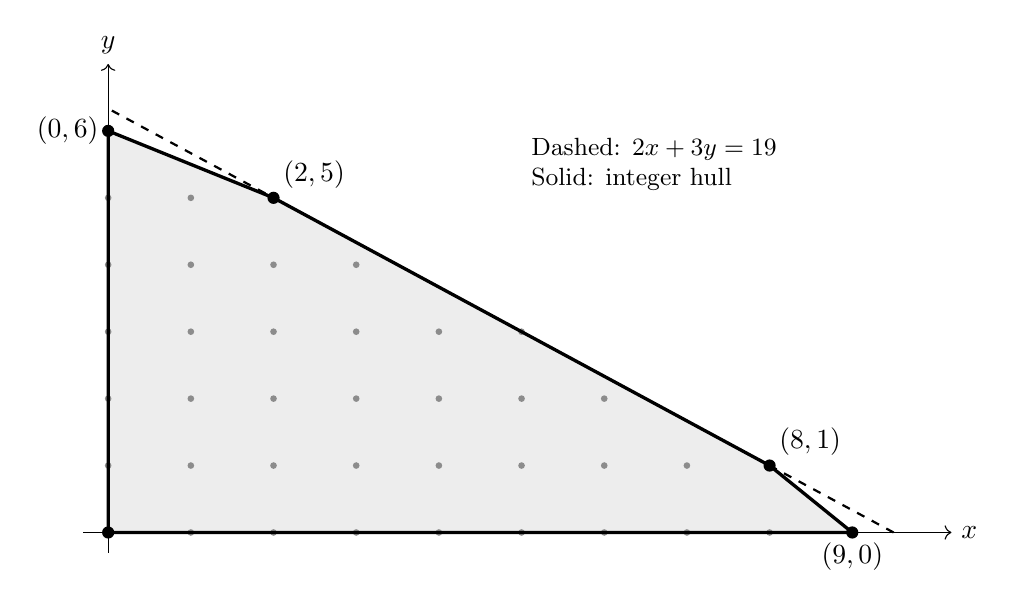
\begin{tikzpicture}[x=1.05cm,y=0.85cm]
 \fill[black!7] (0,0)--(9,0)--(8,1)--(2,5)--(0,6)--cycle;
 \draw[->] (-0.3,0)--(10.2,0) node[right]{$x$};
 \draw[->] (0,-0.3)--(0,7.0) node[above]{$y$};
 \draw[dashed,thick] (9.5,0)--(0,6.3333);
 \foreach \x in {0,...,9} {
   \pgfmathtruncatemacro{\Y}{floor((19-2*\x)/3)}
   \foreach \y in {0,...,\Y} {\fill[black!45] (\x,\y) circle(1.2pt);}
 }
 \draw[very thick] (0,0)--(9,0)--(8,1)--(2,5)--(0,6)--cycle;
 \foreach \x/\y in {0/0,9/0,8/1,2/5,0/6}
   {\fill (\x,\y) circle(2.2pt);}
 \node[below] at (9,0) {$(9,0)$};
 \node[above right] at (8,1) {$(8,1)$};
 \node[above right] at (2,5) {$(2,5)$};
 \node[left] at (0,6) {$(0,6)$};
 \node[align=left,anchor=west,font=\small] at (5,5.5)
 {Dashed: $2x+3y=19$\\Solid: integer hull};
\end{tikzpicture}
\caption{The finite specialization $T=3$, $r=1$. This is an exact ordinary
model illustrating the five-vertex pattern, not a scale drawing of infinite
surreal lengths.}\label{poly:oih:fig:knapsack}
\end{figure}

\subsection{An explicit multiscale instance}

Take the purely infinite parameter
\[
 H=\omega^2+\sqrt3\,\omega+\omega^{1/2},\qquad B=H+13.
\]
Then $B=6T+1$ with $T=H/6+2$. The omnific integer hull has precisely the
five vertices
\begin{equation}\label{poly:oih:eq:multiscale}
 (0,0),\quad (H/2+6,0),\quad(H/2+5,1),\quad
 (2,H/3+3),\quad(0,H/3+4).
\end{equation}
This example carries several scales exactly while the ordinary residue
$13\bmod6$ selects the combinatorial row. The same formulas remain valid if
$H$ is replaced by any positive purely infinite normal form, including one
with infinite support. The example does not rely on the displayed support
having only three terms.

\section{Executable checks and their exact scope}\label{poly:oih:sec:checks}

The accompanying \pathcode{code/12-omnific-hulls-verify.py} uses only Python's standard library. All
geometric decisions are made with integers and \texttt{fractions.Fraction};
no floating-point tolerance appears. It is a finite arithmetic verification
program, not a general implementation of surreal arithmetic and not a proof
assistant certificate.

The supplied run produced the results in Table~\ref{poly:oih:tab:checks}. For every
$B=0,\ldots,245$, the program independently enumerates ordinary lattice points,
computes their monotone-chain convex hull, constructs the 21-label candidate
list, and enumerates the vertices of the cut system. All three hulls agree.
For $B=6T+r$ with $T=2,\ldots,40$, it also verifies the exact six-residue
table. The finite computations support the formulas; the proof for infinite
$T$ is the algebraic argument above, not numerical extrapolation.

\begin{table}[htbp]
\centering
\renewcommand{\arraystretch}{1.2}
\begin{tabularx}{\linewidth}{@{}Xr@{}}
\toprule
Exact check family & Count \\
\midrule
Conformal decompositions for nonzero vectors in $[-80,80]^2$ & 25,920 \\
Finite tests excluding smaller conformal vectors for listed generators & 110 \\
Independent integer-hull comparisons, $0\le B\le245$ & 246 \\
Lattice points enumerated across those instances & 426,236 \\
Checks of the six-residue vertex table, $2\le T\le40$ & 234 \\
Local-versus-global augmentation checks, $0\le B\le35$ & 77,469 \\
Exact rational-square certificates for the irrational example & 4 \\
\bottomrule
\end{tabularx}
\caption{Actual results of the included verification run. The largest vertex
count observed in the knapsack family was five.}\label{poly:oih:tab:checks}
\end{table}

For the last check family, the program certifies
\[
 \frac12-\frac1D<m-\sqrt2\,n<\frac12
\]
for
\[
 (D,n,m)=(10,11,16),\ (100,64,91),\ (1000,781,1105),\
 (10000,12671,17920).
\]
It does so by comparing the rational squares of $m-1/2$ and $m-1/2+1/D$
with $2n^2$. These are exact witnesses of ordinary approach to $1/2$; the
nonexistence of a surreal supremum is proved separately in
\cref{poly:oih:thm:irrational}.

Run the checks from the package directory with
\begin{quote}\ttfamily\small
python code/12-omnific-hulls-verify.py \textbackslash\\
\hspace*{2em}--output /path/to/scratch/verification\_results.json
\end{quote}
The JSON file and the recorded console output are both included. (\wtag{} Source~12 printed \texttt{python verify.py --output}
\pathcode{verification_results.json}, run from its package directory. Without
\texttt{--output} the program writes \texttt{verification\_results.json}
into the current directory; pass a path outside the report directory, as
above, so that the shipped record is never overwritten. The recorded JSON
file and console output are shipped as
\pathcode{data/12-omnific-hulls-verification_results.json} and
\pathcode{data/12-omnific-hulls-verification_output.txt}. The shipped
\pathcode{code/12-omnific-hulls-Makefile} still names the delivery paths
\texttt{verify.py}, \texttt{verification\_results.json},
\texttt{verification\_output.txt} and \texttt{article.tex}. The README of
source~12 adds: ``Do not use Python's \texttt{-O} flag: the comparisons are
implemented as assertions.'') The program
has assertions for every claimed comparison and exits with an error if any
check fails. Completeness of the general Graver construction for arbitrary
matrices is not tested by this one example; its mathematical proof is
\cref{poly:oih:lem:ordinary-decomp}.

\section{Formalization architecture and proof-audit boundaries}\label{poly:oih:sec:formalization}

\noindent\wtag{} This section is a proposal: nothing of this Part is
formalized. The Lean declarations that already cover its first layer are
listed after \cref{poly:oih:tab:formalization}.

\subsection{A field-generic core and a surreal-specific interface}

The positive theorem should be formalized for an integer part of an ordered
field before specializing to surreals. This keeps ordinal and normal-form
machinery out of the finite combinatorial proof. The surreal-specific interface
then supplies flooring, constant extraction, finite-element rigidity, and
closure of purely infinite elements under real scalar multiplication.

A useful implementation split is shown in Table~\ref{poly:oih:tab:formalization}. These
are proposed mathematical contracts, not names of declarations asserted to
exist in the repository. The inspected repository does not by itself certify
any of the new hull theorems in this article.

\begin{table}[htbp]
\centering
\small
\renewcommand{\arraystretch}{1.2}
\begin{tabularx}{\linewidth}{@{}p{0.25\linewidth}X@{}}
\toprule
Proposed layer & Contract to establish \\
\midrule
Integer-part interface & Least positive element, ordinary division and
remainders, floors, and bounded-element rigidity. \\
Presburger bridge & Interpret the fixed additive language in the integer part;
prove transfer of sentences and the bounded-optimization instance. \\
Finite conformal test set & A finite graph-Graver certificate, its ordinary
conformal decomposition theorem, and the fixed-formula transferred version. \\
Optimization and geometry & Feasible unit moves, local optimality, rational
objective cells, finite strict separation, and finite hull generation. \\
Candidate compiler & Full rank of small-slack rows, adjugate candidate formulas,
congruence tests, and extraction of a finite face lattice. \\
Surreal obstruction & The real-vector-space tail splitting, dense real images,
missing suprema, and the integer-right-hand-side infinitesimal example. \\
\bottomrule
\end{tabularx}
\caption{A proposed proof-assistant dependency decomposition.}\label{poly:oih:tab:formalization}
\end{table}

\noindent\wtag{} At the write phase (ProveIt \texttt{HEAD}
\pathcode{4e128356d}) the first row (``Integer-part interface'') is already
proved in Lean for the actual omnific ring, with no \texttt{sorry}:
\pathcode{Surreal.Foundations.SignSequence.omnific_bounded_iff} (an omnific
integer bounded by an ordinary real is an ordinary integer) and
\pathcode{Surreal.Foundations.SignSequence.omnific_least_positive}
(\pathcode{Surreal/Foundations/OmnificUnits.lean}, lines 65 and 104);
\pathcode{Surreal.Foundations.SignSequence.omnificFloor_spec} and
\pathcode{Surreal.Foundations.SignSequence.existsUnique_omnific_integerPart}
(\pathcode{Surreal/Foundations/OmnificFloor.lean}, lines 112 and 138);
\pathcode{Surreal.Foundations.SignSequence.existsUnique_omnific_division}
(ordered division by any positive omnific integer,
\pathcode{Surreal/Foundations/OmnificDivision.lean}, line 62); and
\pathcode{Surreal.Foundations.SignSequence.omnificQuotientZModEquiv}
($\Oz/n\Oz\cong\Z/\lvert n\rvert\Z$,
\pathcode{Surreal/Foundations/OmnificResidues.lean}, line 81). Paths are
relative to \pathcode{Algebra/SurrealNumbers/}. The Presburger bridge and
every later row are not formalized, and nothing in this Part is.

For a universe-relative surreal type, the field-generic theorems avoid
proper-class quantification completely. The full-class interpretation of this
article is recovered by the finite-data localization already proved. These are
two compatible presentations, not a request to introduce a type whose elements
form the collection of all sets.

The repository's ordinary Cooper implementation is especially relevant to the
finite predicates in \cref{poly:oih:thm:parameter-data}. It does not automatically prove
their soundness under omnific interpretation. That soundness is a separate
semantic theorem, after which the same finite syntax can be reused. Likewise,
an executable list of candidate points is not a proof that all vertices occur
in it until the small-slack theorem has been connected to the checker.

\subsection{The five delicate steps}

The following are the principal places where an apparently shorter argument
would be invalid.

\paragraph{Bounded is not finite.}
The boxed lattice slice may be a proper class. Ordinary finite optimization is
used only to prove a Presburger sentence, then transferred with parameters.

\paragraph{Infinite coefficients are not infinitely many steps.}
The decomposition $u=\sum_{g\in\GA}\lambda_g g$ has an ordinary finite index
set. Its coefficients may be infinite. No induction on an omnific norm or
termination of unit augmentation is asserted.

\paragraph{A polytope cannot be assumed before it is constructed.}
Finite optimal representatives and strict separation prove finite generation
before normal-fan or edge arguments are applied to the integer hull.

\paragraph{Small slacks are ordinary.}
The rank argument depends on $s_i<M_i$ with $M_i$ ordinary. Replacing this by
an unspecified surreal slack bound would not give finitely many offsets.

\paragraph{A real limiting value need not be a surreal supremum.}
The irrational example has upper bounds $r-\varepsilon$ for every positive
infinitesimal $\varepsilon$. Its real limiting value is not the least upper
bound in $\No$, and real sequences cannot settle order-topological questions.

\subsection{What has actually been checked}

The mathematical dependencies are explicit: normal-form arithmetic at the
interface, the classical $\Z$-group completeness theorem, finite conformal
integer decompositions, and finite ordered-field linear separation. The
manuscript supplies the remaining arguments. The code checks finite examples
and exact algebraic comparisons. The LaTeX source compiles independently of
the repository. No repository build, new Lean proof, independent peer review,
or exhaustive literature-priority certification is claimed.

\section{Further research questions and topics}\label{poly:oih:sec:questions}

These are proposed next questions for this research program. They are not all
asserted to be previously published open problems; several ask for an explicit
omnific or proof-certified version of a classical construction.

\begin{enumerate}[label=\textbf{Q\arabic*.},leftmargin=2.8em]
\item \textbf{Smaller universal test sets.}
Which proper subsets of the graph Graver set still certify all linear optima
for the fixed matrix $A$ and all omnific right-hand sides? Distinguish sets
sufficient for generic objectives, all face objectives, and just the
small-slack rank argument. A reduction here improves both the fan and the
candidate bound.

\item \textbf{Efficient finite atlases.}
The finite-atlas consequence in Section~\ref{poly:oih:app:atlas} makes the complete
collection of face lattices decidable from a certified test set. Can the atlas
be computed without enumerating all sign and congruence patterns? Determine
which adjacent objective chambers must select the same vertex uniformly in
the parameters and exploit that coalescence.

\item \textbf{Sharp matrix-dependent bounds.}
Find useful sharp or asymptotically sharp bounds for the maximum vertex count
and the minimum necessary offset ranges as functions of the arithmetic of
$A$. The explicit bound $N(A)$ is deliberately robust, not expected to be
optimal. Total unimodularity provides a benchmark where all offset corrections
can be eliminated.

\item \textbf{Unbounded rational-normal polyhedra.}
Extend the finite-certificate presentation to unbounded omnific slices using
finite vertices, lineality data, and recession directions. The target should
specify exactly which sums of an integer hull and a rational recession cone
are meant and handle slices with no vertices. A bare invocation of a classical
Minkowski decomposition does not explain the class-sized arithmetic interface.

\item \textbf{Mixed integer and continuous coordinates.}
For variables in $\Oz^p\times\No^q$, determine a finite certificate theory
that combines real elimination with discrete residues. Establish the precise
conditions under which projection commutes with the mixed integer hull and
whether a fixed rational normal arrangement still suffices.

\item \textbf{Instancewise irrational criteria.}
The universal characterization does not classify individual irrational-normal
instances. The right-hand sides $0$, $1/2$, and $1$ in the two-dimensional
examples already exhibit three different behaviors of the principal objective.
Characterize finite generation using the interaction between real constant
fibers and purely infinite feasible faces, rather than row rationality alone.

\item \textbf{Secondary objectives and ordered hierarchies.}
Generalize \cref{poly:oih:prop:integer-rhs} to a finite hierarchy of real supporting
functionals perturbed by successively smaller surreal coefficients. When does
attainment at every preceding level coexist with failure at the next? Identify
finite conditions guaranteeing that the resulting lexicographic face has an
omnific extremal point.

\item \textbf{Comparison of integer parts.}
The positive theorem holds for arbitrary integer parts, but the obstruction
uses the split real-vector-space tail of $\Oz$. Compare integer hulls for
other integer parts of the same ordered field. Determine which structural
properties of the integer part, beyond its additive Presburger theory, govern
real irrational coefficient systems.

\item \textbf{Effective symbolic surreal domains.}
Implement the candidate compiler for a specified representation supporting
exact floor and equality/order tests on rational linear tail expressions.
Track certificate size as a function of expression size, rather than birthday.
An exact treatment of cancellation is necessary; inspecting only leading
valuation data is insufficient.

\item \textbf{Counting without confusing cardinality and length.}
A literal ordinary cardinality cannot count all points of a proper-class
omnific interval. Seek explicitly axiomatized valuations or specialization
invariants that extend ordinary Ehrhart data on finite rational polytopes.
Any proposed invariant must state its additivity, domain, and relation to
ordinary finite specializations; substituting $\omega$ into a polynomial
is not by itself a cardinality theorem.

\item \textbf{Certified integer optimization in the repository.}
Formalize the semantic Presburger bridge and the small-slack rank theorem,
then connect a candidate-list checker to actual omnific convex hulls. An early
milestone is the full six-residue knapsack table. The next is the field-generic
theorem for arbitrary integer parts, separating code execution from the
trusted completeness argument.

\item \textbf{Functorial and geometric interactions.}
Study how these finite integer hulls behave under rational affine maps,
Minkowski sums, and products, and compare their normal-fan atlas with the
repository's other multiscale polytope constructions. Even over ordinary
integers, taking an integer hull does not generally commute with projection;
seek useful sufficient hypotheses, especially integral or totally unimodular
fiber descriptions.
\end{enumerate}

\noindent\wtag{} Q10 is the counting half of Part~IV's question ``Other
integer parts and unbounded geometry'' (\cref{poly:ehr:sec:questions}),
which this Part answers for integer hulls only
(\cref{poly:oih:cor:integer-parts,poly:oih:thm:candidate,poly:oih:thm:descent}).
The ``repository's other multiscale polytope constructions'' of Q12 now
include the other Parts of this report.

\section{Conclusion}

The decisive finiteness is not finiteness of the feasible lattice collection.
It is finiteness of an ordinary arithmetic test set. A fixed rational matrix
admits one finite conformal certificate; Presburger transfer allows its
multiplicities to become omnific without allowing its list of directions to
become infinite. Rational objective cells then give finitely many supporting
points, and a small-slack rank argument makes those points explicit.

The resulting geometry has a clear boundary. Rational-normal families have
uniformly finite integer hulls, ordinary edge directions, an exact
parameter-to-face-lattice compiler, and same-matrix ordinary realizations of
all their finite combinatorial types. Real irrational normals can instead
produce unattained objectives and missing surreal suprema inside bounded
polytopes. Even an attained principal objective and omnific-integer
right-hand sides do not remove every obstruction.

Thus the non-Archimedean extension is neither an automatic source of new finite
polytope types nor a harmless change of scalars for lattice geometry. It has
an exact rational regime in which finite arithmetic controls all scales, and
an irrational regime in which the arithmetic of constant fibers and the
order structure of purely infinite faces must both be retained.

\section{Finite linear certificates over an ordered field (Appendix~A of source~12)}\label{poly:oih:app:linear}

For clarity, this appendix spells out the linear-algebra facts used in the
proofs. Let $K$ be any ordered field; it need not be Archimedean or real closed.
All systems and matrices in this appendix are finite.

\subsection{Elimination and rational feasibility}

To eliminate one variable $t$ from a system of linear inequalities, divide rows
with nonzero $t$-coefficient by its absolute value and collect lower bounds
$t\ge L_i(x)$ and upper bounds $t\le U_j(x)$. Existence of $t$ is equivalent
to $L_i(x)\le U_j(x)$ for every pair, together with the rows not involving
$t$. Strict inequalities remain strict whenever one of the paired bounds is
strict. Equalities may first be solved or expressed as two weak inequalities.
If only lower or only upper bounds remain, a witness is obtained by adding or
subtracting $1$ from an extremal bound as necessary. If both sides remain,
a midpoint works when a strict gap is required; equal endpoints are allowed
only when both bounds permit equality.

These operations are valid over every ordered field. When all starting
coefficients and constants are rational, back-substitution chooses rational
witnesses. Therefore feasibility of such a system over $K$ implies feasibility
over $\Q$. An arbitrary sign condition $c\cdot g>0$ is an ordinary strict
linear inequality. Thus both versions of \cref{poly:oih:lem:objectives} follow from
this finite procedure, including exact zero signs.

\subsection{Strict separation of a point from a finite hull}

Membership of $s$ in the convex hull of $v_1,\ldots,v_k$ is the feasibility
of
\[
 \sum_i\lambda_i v_i=s,\qquad \sum_i\lambda_i=1,\qquad\lambda_i\ge0.
\]
Finite elimination gives the usual alternative for this system: either it is
feasible, or there are $a\in K^d$ and $t\in K$ such that
\[
 a\cdot v_i+t\ge0\quad\text{for all }i,
 \qquad a\cdot s+t<0.
\]
One way to track the alternative is to retain the nonnegative row combinations
produced during elimination; an infeasible final constant inequality supplies
the displayed multiplier certificate. Equality rows have unrestricted
multipliers because they were entered with both signs. This is the finite
Farkas alternative and uses only field operations and order.
Taking $c=-a$ gives
\[
 c\cdot s>t\ge c\cdot v_i\quad\text{for every }i,
\]
which is exactly the strict separator required in
\cref{poly:oih:thm:finite-hull}.

\subsection{Vertices of a bounded polyhedron}

A short constructive argument gives the finite vertex description used for
total unimodularity. At a point $x$ of a nonempty bounded polyhedron, let the
active-row matrix have rank $r<d$. Choose a nonzero direction $u$ annihilated
by its rows. The feasible scalars $t$ for $x+tu$ form a closed interval in
$K$, obtained from finitely many upper and lower linear bounds. Boundedness
ensures both endpoints are finite. Since every currently inactive row has
positive slack, $0$ is strictly between the two endpoints. At each endpoint
a new active row is independent of the old active rows: a dependent row would
also annihilate $u$ and could not become newly tight along the line.

Thus $x$ is a convex combination of two points of strictly larger active rank.
Repeat at most $d-r$ times along each branch. This is an ordinary finite binary
decomposition ending at points with active rank $d$, namely basis vertices.
There are only finitely many nonsingular row bases. Hence the polyhedron is
the convex hull of finitely many such vertices. The argument also covers a
polyhedron lying in a proper affine subspace, because its active rank simply
starts higher. The same finite elimination and supporting-hyperplane
arguments give the usual exposed-face interpretation for finite polytopes.

\section{An effective finite atlas of all realizable face lattices (Appendix~B of source~12)}\label{poly:oih:app:atlas}

\begin{corollary}[Finite atlas from an ordinary certificate]\label{poly:oih:cor:atlas}
Given an ordinary matrix $A$ together with its complete finite conformal test
set, there is an ordinary terminating procedure that lists all face lattices
of nonempty bounded omnific slices $S(\beta)$, up to isomorphism, and supplies
an ordinary integer right-hand side realizing each listed type. It also computes
the exact maximum vertex count among these slices when any such slice exists.
\end{corollary}
\begin{proof}
Construct the finite predicate list of \cref{poly:oih:thm:parameter-data}. There are
only finitely many possible truth patterns. For each pattern, form its formula
$\Phi(t)$ and ask whether the Presburger sentence
\eqref{poly:oih:eq:descent-sentence} is true over $\Z$. Presburger decidability answers
each question. When the answer is yes, ordinary enumeration of integer tuples
$(t,U,x)$, using the corresponding decidable boundedness and nonemptiness
conditions, eventually finds witnesses; equivalently one can use witness
extraction during elimination. The resulting finite bounded integer slice
has an explicitly computable finite hull and face lattice.

Every surviving pattern is realized over $\Z$, hence over $\Oz$ with the
same boundedness statement by elementary localization. Conversely every
nonempty bounded omnific slice contributes a surviving pattern by
\cref{poly:oih:thm:descent}. Remove isomorphic duplicates by finite face-poset
comparison. Counting vertices in the finite list gives the asserted maximum.
If no pattern survives, there is no nonempty bounded slice.
\end{proof}

For an ordinary right-hand side, why can no new infinite omnific feasible point
invalidate the ordinary boundedness assertion? The boundedness property is
itself the Presburger sentence with those ordinary parameters. Its truth over
$\Z$ transfers to every relevant $D_H$, so such an omnific point cannot
exist. In this special case all feasible omnific coordinates are bounded by an
ordinary integer and are therefore ordinary integers.

This corollary is a decidability and existence-of-algorithm statement, not a
practical running-time claim. It records a consequence that would otherwise
be easy to leave incorrectly listed as an unresolved question. The research
challenge in Q2 is efficient construction and compression of the atlas, not
its bare finiteness or computability from the stated certificate.

\section{Notation and dependency ledger (Appendix~C of source~12)}\label{poly:oih:app:ledger}

\begin{longtable}{@{}p{0.23\linewidth}p{0.72\linewidth}@{}}
\toprule
Notation & Meaning \\
\midrule
\endhead
$\No,\Oz$ & Conway's surreal field and omnific integer subring. \\
$\PiInf$ & Purely infinite additive part; a real vector space, with no
nonzero ordinary-bounded elements. \\
$\ct,\floorOz{\cdot}$ & Ordinary integer constant term on $\Oz$ and
omnific floor on $\No$. \\
$A,\beta=h+z$ & Fixed ordinary integer constraint matrix and floored
omnific right-hand side, split into tail and integer constant. \\
$E_A(u)$ & Graph vector $(u,Au)$, used to require conformity in variables
and row values simultaneously. \\
$\GA$ & Finite conformally minimal graph directions in $\Z^d$. \\
$M_i,N(A)$ & Ordinary slack thresholds and the total bound on candidate labels. \\
$\CA(\beta)$ & Integral feasible basis intersections with bounded ordinary
slack offsets. Not every accepted candidate is necessarily a vertex. \\
$Q_A,\widehat Q_A$ & Finite rational objective representatives for chambers,
respectively all nonempty arrangement sign cells. \\
$L_a=a\cdot\Z^d$ & Real additive image controlling the finite values of a
real objective on omnific points. \\
\bottomrule
\end{longtable}

The proof dependencies of the central conclusions can be read without
following the order of exposition:
\[
 \begin{gathered}
 \text{omnific splitting and ordinary division}
 \ \Longrightarrow\ \text{$\Z$-group localization},\\
 \text{ordinary graph Graver decomposition}
 \ +\ \text{Presburger transfer}\\
 \ \Longrightarrow\ \text{finite augmentation criterion},\\
 \text{ordinary-objective attainment}
 \ +\ \text{finite rational sign cells}
 \ +\ \text{strict separation}\\
 \ \Longrightarrow\ \text{finite hull},\\
 \text{finite hull}\ +\ \text{small-slack rank}
 \ \Longrightarrow\ \text{explicit candidate formula},\\
 \text{candidate formula}\ +\ \text{finite objective comparisons}\\
 \ \Longrightarrow\ \text{tail/residue compiler and same-matrix descent},\\
 \text{real-linear tail splitting}\ +\ \text{dense real subgroup}\\
 \ \Longrightarrow\ \text{irrational obstruction and universal dichotomy}.
 \end{gathered}
\]
The dependence on classical Presburger completeness is explicit, not removed
by the finite numerical checks. The dependence on ordinal normal forms is
confined to the surreal interface and the negative examples, not hidden in
the ordinary Graver certificate.

\part{Beyond finite presentations}\label{poly:part:bf}

\paragraph{Source and scope.}\wtag{} This Part prints, whole,
manuscript~06 of batch~59, printed here as source~13: \emph{Beyond Finite
Surreal Polytopes: Exposed faces, sharp infinitesimal depth, and
finite-description rigidity}, headed ``Surreal geometry / finite and infinite
presentations'', author line ``Prepared for Vladimir Reshetnikov with
ChatGPT'' (the PDF metadata of the delivered file reads the same), dated
30~September 2026 (archive \pathcode{Beyond_Finite_Surreal_Polytopes.zip},
main file \pathcode{Beyond_Finite_Surreal_Polytopes/article.tex}; delivered
PDF of 26 pages on Letter paper, not shipped). It was written against
ProveIt commit \pathcode{6996fee43}; it arrived in commit
\pathcode{ed80eba06} and was placed in commit \pathcode{f2cb2034e}. Its
program, recorded run, recorded console output and build file are shipped as
\pathcode{code/13-beyond-finite-verify.py},
\pathcode{data/13-beyond-finite-verification_results.json},
\pathcode{data/13-beyond-finite-verification_stdout.txt} and
\pathcode{code/13-beyond-finite-Makefile}; its three notes, delivered in a
directory \pathcode{notes/}, are shipped as
\pathcode{13-beyond-finite-SOURCES_AND_SCOPE.md},
\pathcode{13-beyond-finite-PROOF_AUDIT.md} and
\pathcode{13-beyond-finite-BUILD_REPORT.md} (whose SHA-256 lines describe the
delivered \pathcode{article.tex} and \pathcode{article.pdf}, neither of which
is shipped). Its README and checksum list \pathcode{SHA256SUMS.txt} are not
shipped; they survive in the delivery archive of arrival commit
\pathcode{ed80eba06}, and the README's status section is printed below.
Every section, result, proof, example, remark, figure, table and research
question of the manuscript is printed here, in the manuscript's order, with
three structural changes: its two appendices are printed as the ordinary
\cref{poly:bf:app:notation,poly:bf:app:provenance} at the end of this Part;
its bibliography is printed as the list ``References of Part~X''; and its
theorem environments are the report's (source~13's \texttt{aliascnt} setup
is dropped; as in the source, all numbered statements share one counter).
Its formalization route (the subsection ``A practical Lean decomposition''
of \cref{poly:bf:sec:verification}) stays in this Part. In this Part ``this
manuscript'' and ``the package'' mean source~13 and its delivery.

\emph{Relation to the other Parts.} Source~13 continues Part~III's question
``Beyond finite vertex sets'' (\cref{poly:mv:sec:research}) and partly
answers it: with set-sized presentations, a class that is both a small hull
and a small halfspace intersection has finite subpresentations of both
(\cref{poly:bf:thm:rigidity}), so definable small hulls and definable small
H-classes are finite polytopes
(\cref{poly:bf:cor:defV,poly:bf:cor:defH}), while the rational moment hull
and its polar are explicit non-polytopal small classes
(\cref{poly:bf:thm:moment,poly:bf:thm:momentpolar}); the volume half of that
question is untouched. It also continues Part~I's scalar-extension
correction (\cref{poly:sec:corrections}, subsection ``A real face and its
scalar extension are different sets''): \cref{poly:bf:cor:basechange}
extends the trace correspondence of faces to arbitrary \emph{sets} of
generators, and the paragraph after it keeps the same warning that a single
exposing functional need not descend. Its exposing normals are surreal, so
it is consistent with Part~V's vertex invisible to all real objectives
(\cref{poly:ic:ex:normal}); its polarity theorem (\cref{poly:bf:thm:polar})
concerns infinite presentations and is complementary to Part~I's finite
polar residue (\cref{poly:ts:prop:polar}). Its opening observation that a
finite list of surreal coordinates produces no new finite face lattice is
the report's ``no new finite face lattices'' spine (\cref{poly:thm:general}).
Source~13 credits the lexicographic exposure theorem, the degree of
non-exposedness and its codimension bound to Mart\'inez-Legaz (1997); its
\cref{poly:bf:thm:degree} is a translation of that invariant, as it says in
\cref{poly:bf:sec:intro}. Its positive theorems are proved for $\No$ in a
fixed universe and, with ``set'' replaced by ``of cardinality less than
$\kappa$'', for every $\kappa$-saturated real closed field
(\cref{poly:bf:thm:kappa}).

\paragraph{Notation in this Part.}\wtag{} The following symbols and
words mean something different elsewhere in the report
(\cref{poly:sec:notation}); the Part-local meaning is the one in force here.
No symbol of source~13 has been renamed.
\begin{itemize}
\item \emph{Small} means indexed by a set in one fixed universe of NBG set
  theory with Global Choice (\cref{poly:bf:sec:foundation}); in
  \cref{poly:bf:thm:kappa} it means of cardinality less than $\kappa$. The
  size condition concerns generators, rows, parameters and formulas. The
  tempting false reading is that a small hull $\VC S$ or a small H-class is
  itself a set: it is in general a proper class, since the hull of two
  distinct points already contains a copy of the surreal interval $[0,1]$.
\item $\VC S=\conv_{\No}S$ (finite convex combinations, $S$ a set) and
  $\HC(A,b)$ (a set-indexed intersection of closed halfspaces). The
  sans-serif $\mathsf V$ is neither Part~III's mixed volume
  $\operatorname{V}$ nor Part~I's dependence space $V$.
\item \emph{Closed} and \emph{bounded} are pointwise order-box notions;
  ``bounded'' means contained in a box of some \emph{surreal} radius, not a
  real one (contrast Part~IV's real box). $\mathcal O$ is the ring of finite
  surreals, the report's $\OO$.
\item $\eps$ is any positive element infinitesimal relative to $\R$, not
  necessarily $\omega^{-1}$; the $\eta$ of \cref{poly:bf:sec:examples}
  ranges over positive infinitesimals and is not $\omega^{-\omega}$.
\item \emph{Degree}: $m_\eps(C,F)$ and $\delta_C(F)$ in
  \cref{poly:bf:thm:degree} are the degree of non-exposedness of a real
  face, a third notion of degree in this report (see the paragraph after
  that theorem); $r_C(F)$ is an exposed-chain length, and $\delta$ is also
  a radius in \cref{poly:bf:cor:closed}.
\item $m_d(t)$ is the moment curve, $M_d$ its rational hull, $H_d$ the polar,
  and $F_A$, $G_A$ their faces, with $k=\lfloor d/2\rfloor$; this $G_A$ is not
  the Graver set $\GA$ of Part~IX or Part~I's Graver basis $G_A$, and $m_d$,
  $m_\eps$ are not Part~I's rank $m$. $K_d$ is the compact real ``paraboloid
  tower'' of \cref{poly:bf:sec:sharp}; $K$ elsewhere is an ordered field.
\item $\upc C=\conv_{\No}(C(\R))$ is the generator extension of a real
  convex set; it is generally not the definable extension $C(\No)$.
\end{itemize}

\paragraph{Abstract of source 13.}
Finite polytope theory over the surreal numbers is governed by ordered-field
algebra. A different phenomenon appears when one permits a set of generators
or a set of inequalities while retaining all surreal scalars. We prove a
finite-description rigidity theorem: if a finite-dimensional convex class is
both the finite-convex-combination hull of a set of surreal points and the
intersection of a set of surreal halfspaces, then both original presentations
reduce to finite subpresentations. More generally, a small definable
intersection contained in a small convex hull admits a finite sandwich.

The same saturation principle gives strong separation of disjoint
set-generated hulls, exposes every nonempty proper face, and forces every nonempty face
of a set-presented halfspace intersection to be cut out by at most $d$ active
input inequalities. Polarity turns nonfinite generation into a genuine
set-versus-class obstruction. We also identify polynomial infinitesimal
exposure degree with the classical degree of non-exposedness, construct
explicit compact examples attaining every codimension bound, and classify
all faces of the hull of the rational moment curve and of its polar.
The hull has only simplex faces on at most $\lfloor d/2\rfloor$ rational
parameters; the polar has no faces below dimension $\lceil d/2\rceil$.

All claims are proved in a fixed class-theoretic universe. The crucial
restriction is that the presentations are sets, not proper classes. This is
an unrefereed research manuscript, not a Lean-certified development; priority
of the new formulations and consequences has not been established.

\paragraph{Title page of source 13.}
A companion research direction for \repo, with explicit provenance,
proof dependencies, counterexamples, and reproducible finite checks.

\paragraph{Status and important distinctions (README of source 13).}
This is an AI-assisted, unrefereed proof manuscript. Its main conclusions
have written proofs, but they are not Lean-certified or independently
refereed. Priority of the proposed geometric formulations and consequences
has not been established. No named longstanding conjecture is claimed solved.

Mart\'inez-Legaz's 1997 lexicographical exposure theorem, classical degree of
non-exposedness, and codimension bound are credited as prior results. The
new polynomial notation does not create a new real invariant. Saturation,
real closedness, finite Farkas theory, and the compactness mechanism are
also prior mathematical tools.

``Small'' means externally set-indexed in one fixed universe. The convex
classes themselves are generally proper classes. Convex combinations have
ordinary finite support. A hull of the real points of a convex body is NOT
its full semialgebraic extension to all surreal points.


\section{The question beyond finite polytopes}\label{poly:bf:sec:intro}

A finite list of surreal coordinates does not, by itself, produce an
unprecedented finite face lattice. Finite linear feasibility, affine
dependence, and the vertex--halfspace correspondence are algebraic facts
about ordered fields. Their validity is not tied to Archimedean scalars.
The ordered-field Farkas theory has both a classical literature and recent
formal verification in Lean~\cite{bf:charnes,bf:dvorak}.

The productive change of question is therefore not merely to replace a
finite real vertex matrix by a finite surreal matrix. It is to ask what
happens when the \emph{presentation} is allowed to be an arbitrary set,
while the ambient scalars range over the entire proper class $\No$.
Two apparently natural generalizations then diverge:
\begin{align}
 \VC S&=\conv_{\No}S,
 &&S\subseteq\No^d\text{ a set},\label{poly:bf:eq:Vintro}\\
 \HC(A,b)&=\bigcap_{i\in I}\{x\in\No^d:a_i\cdot x\le b_i\},
 &&I\text{ a set}.\label{poly:bf:eq:Hintro}
\end{align}
Every convex combination in \eqref{poly:bf:eq:Vintro} has ordinary finite support.
No infinite sum or completion is intended.

\begin{important}{The central answer}
For nonempty classes in ordinary finite dimension,
\[
 \boxed{\text{small V-classes}\ \cap\ \text{small H-classes}
 \ =\ \text{finite polytopes}.}
\]
Moreover, equality of the two presentations forces finite sublists of
\emph{those very presentations} to define the same polytope.
\end{important}

This is not the assertion that every closed bounded surreal convex class is
a polytope. Quite the opposite: we construct closed bounded, countably
generated convex classes with infinitely many vertices and very sparse
face dimensions. They have no set-sized halfspace presentation whatsoever.
On the dual side, a countable intersection of closed bounded intervals can
have no extreme points at all.

\subsection{Relation to the repository}
The consulted \repo\ material includes the surreal-number project overview
and its report on surreal fields across universes~\cite{bf:repo,bf:repouniv}.
The overview distinguishes its constructed, formally checked field
foundations from research reports whose statements are not automatically
machine-checked. The across-universes report studies omitted cuts and the
saturation of old surreal fields; its own README explicitly does not claim
Lean verification. That is the relevant bridge: our geometric mechanism is
\emph{small-cut realization in the full current-universe field}, not a new
assumption of metric compactness.

The proofs below do not import any unrefereed theorem from the repository.
They use the classical real-closedness and cut properties of $\No$, finite
ordered-field convexity, and first-order compactness. They can therefore be
reviewed independently of the repository's other research claims. The
source notes record the consulted paths and the indexed commit
(\wtag{} shipped as \pathcode{13-beyond-finite-SOURCES_AND_SCOPE.md}). No
repository build or axiom audit was performed for this manuscript.

\subsection{What is established, and what is not claimed}
The main results and their logical roles are as follows.
\begin{center}
\small
\begin{tabular}{@{}>{\raggedright\arraybackslash}p{.23\textwidth}>{\raggedright\arraybackslash}p{.69\textwidth}@{}}
\toprule
Result & Precise content\\
\midrule
Separation and exposure & Disjoint small hulls admit a uniform surreal
separator; every nonempty proper face of a small hull is exposed
(\cref{poly:bf:thm:separate,poly:bf:thm:Vface}).\\[4pt]
Finite active faces & Every nonempty face of a small halfspace intersection is an
intersection with at most $d$ active input hyperplanes
(\cref{poly:bf:thm:active}).\\[4pt]
Double compression & A small V/H equality reduces simultaneously to finite
subpresentations (\cref{poly:bf:thm:rigidity}).\\[4pt]
Polar obstruction & A nonpolyhedral small hull with the origin interior has
a polar not generated by any set of points (\cref{poly:bf:thm:polar}).\\[4pt]
Exact exposure degree & Polynomial degree in one infinitesimal equals
Mart\'inez-Legaz's classical degree of non-exposedness; an explicit compact
family attains the bound (\cref{poly:bf:thm:degree,poly:bf:thm:sharp}).\\[4pt]
Moment-curve faces & The proper face lattice of the rational moment hull is
exactly its $\lfloor d/2\rfloor$-point simplex skeleton; the polar has
a complementary dimension gap (\cref{poly:bf:thm:moment,poly:bf:thm:momentpolar}).\\
\bottomrule
\end{tabular}
\end{center}

The lexicographical exposure theorem, its degree invariant, and its
codimension bound were already proved by Mart\'inez-Legaz in
1997~\cite{bf:martinez}. We explicitly credit them. Our infinitesimal degree
statement is a translation and application of that theory, not a claim to
have discovered the invariant. The finite-compression arguments are
applications of familiar model-theoretic compactness. Their geometric
combination, sharp examples, and class-size consequences are the research
contribution proposed here; an exhaustive priority review remains to be
done. No named longstanding conjecture is asserted to have been settled.

\section{Size conventions and the saturation engine}\label{poly:bf:sec:foundation}

\subsection{One universe, ordinary finite dimension}
We work in a fixed universe of NBG set theory with Global Choice. The field
$\No$ is a proper class, and each individual surreal is a set-coded number.
The integer $d\ge1$ is always an ordinary finite natural number. A
\emph{small} family means a family indexed by a set in this universe.
A small family can be uncountable, and its parameters can have very large
birthdays. A family of definable classes is understood through a set of
formula-and-parameter codes, not as a set whose members are proper classes.
Likewise, a face lattice described below is represented by the set of
facial traces or finite affine-span codes, with its inclusion relation.

A subclass of $\No^d$ is convex when it is closed under all two-point convex
combinations with coefficients in $\No$. A face is a convex subclass $F$ of
a convex class $C$ such that
\[
 x,y\in C,\quad 0<t<1,\quad (1-t)x+ty\in F
 \quad\Longrightarrow\quad x,y\in F.
\]
The empty face and $C$ itself are included. An exposed proper face has the
form $\{x\in C:u\cdot x=c\}$, where $u\ne0$ and $u\cdot C\le c$.

For $x\in\No^d$, let $\norm{x}_\infty=\max_j|x_j|$. We call a class
\emph{closed} when every point outside it has a disjoint positive-radius
open box, and \emph{bounded} when it is contained in a box of some surreal
radius. These are pointwise descriptions; we do not treat the collection of
all open subclasses as an ordinary set topology. Relative interior is
defined in the same way inside the affine hull.

\begin{scopebox}
\textbf{A small presentation is not a small convex class.}
A hull of two distinct points already contains a copy of the entire surreal
interval $[0,1]$, a proper class. For example, that interval contains distinct
$\omega^{-\alpha}$ for all positive ordinals $\alpha$. All size restrictions
below concern generators, rows, parameters, or formulas---not the elements
of the convex hull.
\end{scopebox}

\subsection{Cuts and relative embeddings}
The classical surreal cut property says that for sets $L,R\subseteq\No$
with $L<R$, there is $z\in\No$ such that $L<z<R$, including when either side
is empty. We also use that $\No$ is real closed. The relationship between
these facts, universality, and absolute saturation is developed in
Ehrlich's work~\cite{bf:ehrlich}; fields of surreal numbers are studied further
in~\cite{bf:vdde}.

\begin{lemma}[Relative embedding]\label{poly:bf:lem:embedding}
Let $K\subseteq\No$ be a set-sized real closed subfield, and let $E/K$ be a
set-sized ordered real closed field extension. There is an ordered-field
embedding $E\hookrightarrow\No$ that is the identity on $K$.
\end{lemma}
\begin{proof}
Well-order the elements of $E$. Construct embeddings of real closed
intermediate subfields by recursion through this set-sized well-order.
At a successor stage, an element not in the present real closed field $F$
is transcendental over $F$. Its position determines a cut of $F$: the two
sets of elements below and above it partition $F$. Transport this cut to
the image of $F$ and realize it in $\No$.

The cut-realizing number is not in the image of $F$, since every element of
that image lies on one side of the cut. It is therefore transcendental over
that real closed image. The resulting map on $F(a)$ preserves order:
a polynomial over a real closed field factors into real linear factors
and quadratic factors of fixed sign, so the cut determines the signs of
all its nonzero values at a transcendental element. Extend this embedding
to the ordered real closure of $F(a)$ inside $E$ and $\No$. Ordered real
closures are unique up to ordered isomorphism over the base. At a limit
stage take the union; a union of a chain of real closed fields is real
closed. The recursion has set length, so all cuts used are sets.
\end{proof}

\begin{theorem}[Small-type realization]\label{poly:bf:thm:saturation}
Let $p(x)$ be a set of ordered-field formulas in a fixed finite tuple of
variables, with a set of parameters from $\No$. If every finite subset of
$p$ has a solution in $\No$, then all of $p$ has a solution in $\No$.
\end{theorem}
\begin{proof}
Put all parameters in a set-sized real closed subfield $K\subseteq\No$.
For each finite conjunction from $p$, its existential closure is true in
$\No$. Quantifier elimination for real closed fields makes that sentence
equivalent to a quantifier-free statement over $K$, and hence true in $K$.
This use of quantifier elimination is pointwise; no set-sized model with
underlying domain $\No$ is being postulated.

Apply ordinary first-order compactness to the elementary diagram of $K$
and the formulas $p$ with new constants for $x$. A set-sized elementary
extension $E$ realizes them. It is a real closed ordered extension of $K$.
Embed $E$ in $\No$ over $K$ by \cref{poly:bf:lem:embedding}. Quantifier elimination
again makes this embedding elementary for ordered-field formulas, so the
image of the realizing tuple realizes $p$.
\end{proof}

We will repeatedly use two special cases. A small collection of positive
surreals has a positive strict lower bound, and a small collection of
surreals has a strict upper bound. These are immediate cuts. Less
obviously, infinitely many simultaneous linear equations, inequalities,
and nonmembership conditions can be solved whenever all finite
subcollections can.

\begin{remark}[What saturation does not say]
The theorem gives realization for a \emph{set} of formulas. Replacing that
set by a proper class is invalid. Nor may one silently replace the full
current-universe $\No$ by an arbitrary birthday cutoff or by an old field
$\No^M$ viewed from a larger universe. Section~\ref{poly:bf:sec:cardinal} isolates
the precise hypothesis needed in those settings.
\end{remark}

\section{Finite convexity and facial traces}\label{poly:bf:sec:finite}

\subsection{The finite algebraic backbone}
We recall the finite results used below. Over an ordered field, a point in a
convex hull in dimension $d$ is a combination of at most $d+1$ generators.
Indeed, if a positive-support representation has more terms, choose an
affine dependence $(\mu_j)$, so that $\sum\mu_j=0$ and
$\sum\mu_j s_j=0$. After changing sign, some $\mu_j>0$. Subtract
$\min_{\mu_j>0}\lambda_j/\mu_j$ times that dependence from the coefficients.
At least one coefficient vanishes and none becomes negative. Iterate.
This is the usual algebraic proof of Carath\'eodory's theorem.

Finite systems of linear inequalities admit Fourier--Motzkin elimination:
a variable with lower and upper bounds is eliminated by all pairwise
comparisons of those bounds. Strict bounds are retained when appropriate.
Only field arithmetic and order are involved. Its consequences include
finite Farkas alternatives, invariance of finite linear feasibility under
ordered-field extensions, and finite polyhedral descriptions of finite
convex hulls. The finite vertex--halfspace theorem for bounded polyhedra
and exposure of all finite-polytope faces are used in their standard
ordered-field form~\cite{bf:charnes,bf:dvorak}.

For separation alone it would also suffice to use real-closed-field
transfer: for fixed finite numbers of vertices and a fixed dimension, the
assertion that two disjoint finite hulls have a strict separator is a
first-order statement true over $\R$.

\begin{lemma}[Finite ingredients]\label{poly:bf:lem:finite}
In finite dimension over an ordered field, the following hold.
\begin{enumerate}[label=(\roman*)]
\item Disjoint nonempty finite convex hulls admit a strict affine separator.
The separator can be rescaled to have any specified positive finite-list
margin.
\item Every nonempty proper face of a finite polytope is exposed.
\item If $P=\{x:a_i\cdot x\le b_i,\,i\in J\}\ne\varnothing$ with $J$
finite, then $v\cdot x\le\beta$ is valid on $P$ exactly when
\[
 v=\sum_{i\in J}\lambda_i a_i,\qquad
 \sum_{i\in J}\lambda_i b_i\le\beta,\qquad \lambda_i\ge0.
\]
\end{enumerate}
\end{lemma}

\subsection{A face is determined by its generators}
\begin{lemma}[Trace and affine hull]\label{poly:bf:lem:trace}
Let $C=\conv_K S$ over an ordered field $K$, and let $F$ be a nonempty face.
Then
\[
 F=\conv_K(S\cap F),\qquad F=C\cap\aff_K F.
\]
Every nonempty finite-dimensional convex class has a relative interior
point. In particular, a face has one.
\end{lemma}
\begin{proof}
In a finite convex combination belonging to a face, every generator with
positive coefficient belongs to that face. This follows by isolating one
coefficient and applying the segment definition; the single-coefficient
case is immediate. It proves the first equality.

Choose an affinely independent finite set spanning the affine hull of a
nonempty convex class. Its simplex lies in the class, and its barycenter contains a relative
open box in the affine span, as is seen from its strictly positive
barycentric coordinates. This proves the relative interior assertion using
only finite inequalities.

Choose $p\in\ri F$ and $x\in C\cap\aff F$. For sufficiently small $t>0$,
$y=p-t(x-p)$ lies in $F$. The point $p$ is an interior point of the segment
$[x,y]$ unless $x=p$. The face property gives $x\in F$, proving the second
equality.
\end{proof}

\begin{proposition}[Finite character of facial traces]\label{poly:bf:prop:facial}
For $I\subseteq S$, the following are equivalent:
\begin{enumerate}[label=(\roman*)]
\item $I=S\cap F$ for a face $F$ of $\conv_K S$.
\item For every finite $T\subseteq S$, there is an affine function over $K$
that is zero on $T\cap I$ and strictly negative on $T\setminus I$.
\end{enumerate}
Under these conditions, $F=\conv_K I$. The empty and full traces are allowed.
\end{proposition}
\begin{proof}
If $F$ exists, its intersection with $\conv_K T$ is a face of that finite
polytope, generated by $T\cap I$. Finite exposure gives the affine function
when this face is nonempty and proper. Use the constant functions $-1$ and
$0$ in the empty and full cases.

Conversely, a point of $S\setminus I$ cannot belong to $\conv_K I$: a
hypothetical expression would involve only finitely many generators, and
the corresponding affine function would be both negative and zero there.
Thus the trace of $\conv_K I$ is exactly $I$.

Suppose an interior point of a segment $[x,y]$ in $\conv_K S$ belongs to
$\conv_K I$. Gather the finite generators in expressions for $x$, $y$, and
that point into one finite set $T$. The affine function for $T$ is
nonpositive at $x,y$ and zero at their strict convex combination. Both
values are zero. In the chosen representations of $x,y$, all generators
with positive weight must therefore belong to $I$. Thus $x,y\in\conv_K I$.
\end{proof}

\begin{corollary}[Scalar extension preserves faces]\label{poly:bf:cor:basechange}
For an ordered-field extension $K\subseteq L$ and a set $S\subseteq K^d$,
the face lattices of $\conv_K S$ and $\conv_L S$ correspond canonically by
their traces on $S$. Face dimensions are preserved. In particular,
\[
 F\longmapsto\conv_L(S\cap F)
\]
is an inclusion-preserving bijection of faces.
\end{corollary}
\begin{proof}
The finite systems in \cref{poly:bf:prop:facial} are feasible over $K$ if and only
if they are feasible over $L$, by finite linear elimination. The trace
criterion therefore gives the same collection of subsets of $S$ in both
fields. Affine ranks of finite matrices over $K$ do not change after scalar
extension.
\end{proof}

Although the face lattice is preserved, the existence of a \emph{single}
exposing functional is an infinite system and need not descend to $K$.
That distinction is essential later.

\noindent\wtag{} Part~I makes the same distinction for a finite list of real
vertices (\cref{poly:sec:corrections}, subsection ``A real face and its
scalar extension are different sets''); \cref{poly:bf:cor:basechange}
extends the face correspondence to an arbitrary set of generators.

\section{Separation, closedness, and exposure of small hulls}\label{poly:bf:sec:V}

\begin{theorem}[Uniform strong separation]\label{poly:bf:thm:separate}
Let $S,T\subseteq\No^d$ be nonempty sets such that
$\VC S\cap\VC T=\varnothing$. There exist $u\in\No^d\setminus\{0\}$ and
$c\in\No$ with
\[
 u\cdot s\le c-1\quad(s\in S),\qquad
 u\cdot t\ge c+1\quad(t\in T).
\]
The same inequalities hold throughout the two hulls.
\end{theorem}
\begin{proof}
View the displayed inequalities as a type in the $d+1$ unknowns $(u,c)$.
Every finite subsystem concerns disjoint finite hulls. Add one fixed
generator from each side if a side is absent from that subsystem. Apply
\cref{poly:bf:lem:finite}(i) and rescale a strict separator around the midpoint of
its finite gap so that both margins are at least $1$. Thus every finite
subsystem is feasible. By \cref{poly:bf:thm:saturation}, the whole type is
realized. Since both $S$ and $T$ are nonempty, its solution cannot have
$u=0$. Finite convex combinations preserve the inequalities.
\end{proof}

\begin{corollary}[Bounded and closed]\label{poly:bf:cor:closed}
Every small hull $\VC S$ is order bounded and closed. For each exterior
point there is a strictly separating affine halfspace, and consequently
\[
 \VC S=\bigcap\{H:H\text{ is a closed affine halfspace containing }\VC S\}.
\]
The intersection on the right is generally proper-class indexed.
\end{corollary}
\begin{proof}
A surreal $M$ strictly greater than all $|s_j|$ exists because this is a set
of coordinates. Every finite convex combination is contained in
$[-M,M]^d$.

For $x\notin\VC S$ with $S$ nonempty, apply \cref{poly:bf:thm:separate} to $S$
and $\{x\}$. If $\norm{y-x}_\infty<\delta$, where
\[
 \delta=\frac{1}{1+\sum_j|u_j|},
\]
then $|u\cdot(y-x)|<1$. Hence this open box around $x$ misses $\VC S$.
The separating halfspace also excludes $x$, proving the intersection
formula. Empty hulls satisfy the assertions directly.
\end{proof}

Boundedness here means bounded by a surreal, not by an ordinary real.
Closedness says nothing about attainment of infima or about finite
subcovers of arbitrary open covers.

\begin{theorem}[All small-hull faces are exposed]\label{poly:bf:thm:Vface}
Let $C=\VC S$ for a set $S\subseteq\No^d$, and let $F$ be a nonempty proper
face of $C$. Put $I=S\cap F$. There are $u\ne0$ and $c$ such that
\begin{align*}
 u\cdot i&=c &&(i\in I),\\
 u\cdot s&\le c-1 &&(s\in S\setminus I).
\end{align*}
In particular, $F=\{x\in C:u\cdot x=c\}$.
\end{theorem}
\begin{proof}
By \cref{poly:bf:lem:trace}, $F=\VC I$, so $I$ is nonempty; $S\setminus I$ is
also nonempty because $F$ is proper. A finite subsystem of the displayed
equations and inequalities concerns a finite set $T\subseteq S$. Add
fixed elements of $I$ and $S\setminus I$ to $T$. The nonempty proper face
$F\cap\VC T$ of the finite polytope $\VC T$ is exposed. Its finitely many
outside generators have strictly positive slack. Rescale by the reciprocal
of their minimum slack. This satisfies the finite subsystem.

Realize the entire type by \cref{poly:bf:thm:saturation}. For
$x=\sum_j\lambda_j s_j\in C$, its slack satisfies
\[
 c-u\cdot x\ \ge\ \sum_{s_j\notin I}\lambda_j.
\]
It is zero for $x\in\VC I$, and zero slack in any representation forces all
positively weighted generators to belong to $I$. This proves the claimed
exposed-face identity. The outside inequalities force $u\ne0$.
\end{proof}

\begin{remark}[The margin is a generator margin]
There is no positive uniform gap on all of $C\setminus F$. If $p\in F$
and $s\notin F$, points $(1-t)p+ts$ approach $F$ as $t>0$ decreases. The
unit margin in \cref{poly:bf:thm:Vface} concerns the specified outside generators.
Confusing these two assertions would make the theorem false even for an
ordinary segment.
\end{remark}

\begin{corollary}[Number of faces]\label{poly:bf:cor:countfaces}
Every extreme point of $\VC S$ belongs to $S$. Every nonempty face is
determined by the affine hull of at most $d+1$ elements of $S$. Thus its
face collection is set-indexed, and if $S$ is infinite it has at most
$|S|$ faces.
\end{corollary}
\begin{proof}
A singleton face is generated by its trace, so its point belongs to $S$.
For any nonempty face choose at most $d+1$ generators spanning its affine
hull; \cref{poly:bf:lem:trace} recovers the face by intersection with that affine
hull. There are only $|S|$ finite subsets of an infinite set $S$.
\end{proof}

\section{Small halfspace systems: certificates and active faces}\label{poly:bf:sec:H}

Fix a set $I$ and a system
\[
 H=\{x\in\No^d:a_i\cdot x\le b_i\text{ for every }i\in I\}.
\]
The rows may be redundant, and zero rows are permitted.

\begin{theorem}[Finite certificates from small systems]\label{poly:bf:thm:certificates}
The following statements hold.
\begin{enumerate}[label=(\roman*)]
\item If $H=\varnothing$, some finite subsystem is infeasible.
\item If $H\subseteq\{x:v\cdot x\le\beta\}$, the same implication already
holds for a finite subsystem of the original rows.
\item If $H\ne\varnothing$, every valid inequality has a finite Farkas
certificate:
\[
 v=\sum_{i\in J}\lambda_i a_i,\qquad
 \sum_{i\in J}\lambda_i b_i\le\beta,
 \qquad J\subseteq I\text{ finite},\quad\lambda_i\ge0.
\]
\end{enumerate}
\end{theorem}
\begin{proof}
For (i), finite feasibility of all rows would imply feasibility by
\cref{poly:bf:thm:saturation}. For (ii), if no finite subsystem implied the desired
inequality, the type consisting of every input row together with
$v\cdot x>\beta$ would be finitely satisfiable. Its realization would
contradict validity. For (iii), the finite subsystem supplied by (ii) is
nonempty because it contains $H$. Apply finite Farkas theory to it.
\end{proof}

This is a finiteness theorem for \emph{each consequence}, not a finiteness
theorem for the entire row system. Different consequences may require
different finite sublists.

\subsection{A uniform neighborhood in the active affine space}
At $x\in H$, define
\[
 A(x)=\{i\in I:a_i\cdot x=b_i\},\qquad
 W_x=\bigcap_{i\in A(x)}\ker a_i.
\]
The inactive slacks form a set of positive numbers. A single positive
surreal can be chosen smaller than all their suitably normalized values.
This eliminates the familiar real phenomenon of infinitely many nearly
active inequalities creating a new local boundary without an active row.

\begin{theorem}[Finite active-face theorem]\label{poly:bf:thm:active}
For each $x\in H$, choose $J\subseteq A(x)$ whose normals span all the
active normals. It can be chosen with $|J|\le d$. Then
\[
 F_x=H\cap\bigcap_{i\in J}\{y:a_i\cdot y=b_i\}
\]
is the minimal face of $H$ containing $x$, and $x\in\ri F_x$.
Every nonempty proper face of $H$ is such a slice. It is exposed by the
sum of at most $d$ of the original row normals.
\end{theorem}
\begin{proof}
For each inactive row let $s_i=b_i-a_i\cdot x>0$. Choose $\delta>0$ with
\[
 \delta<\frac{s_i}{1+\sum_{j=1}^d|a_{ij}|}
 \qquad(i\notin A(x)).
\]
The cut property gives such a $\delta$; if there are no inactive rows, take
any positive $\delta$. If $w\in W_x$ and $\norm w_\infty<\delta$, all active
rows remain equalities and all inactive rows remain satisfied. Thus
$x+(W_x\cap(-\delta,\delta)^d)\subseteq H$.

Finite-dimensional linear algebra gives the stated $J$. Its common kernel
is $W_x$, so the displayed slice has affine hull $x+W_x$ and contains a
relative neighborhood of $x$. Each active equality cuts out a face, and
therefore $F_x$ is a face. If another face $G$ contains $x$, then for every
$y\in F_x$ the small relative neighborhood permits a point of $F_x$ just
beyond $x$ on the line from $y$ to $x$. The face property at $x$ forces
$y\in G$. Hence $F_x$ is minimal.

For an arbitrary nonempty face $F$, choose $x\in\ri F$ using
\cref{poly:bf:lem:trace}. The same line argument shows that every face containing
$x$ contains $F$, so $F=F_x$. Finally, all the slacks of the rows in $J$
are nonnegative on $H$. Their sum vanishes exactly when each vanishes.
Thus the sum of their normals exposes the slice. If the slice is proper,
that sum cannot be zero: evaluated at $x$, a zero summed normal would give
zero summed bound and force the summed slack to vanish everywhere on $H$.
\end{proof}

\begin{corollary}[Vertices come from active bases]\label{poly:bf:cor:Hvertices}
A point $x\in H$ is extreme if and only if its active row normals span
$\No^d$. Equivalently, $x$ is the unique solution of $d$ independent active
input equations. Consequently $\ext H$ is a set.
\end{corollary}
\begin{proof}
The minimal face at $x$ has direction space $W_x$ and a relative
neighborhood in that space. It is a singleton precisely when $W_x=0$.
Independent $d$-tuples of rows are set-indexed, and each has at most one
solution, given by a finite matrix inverse. Their feasible solutions form
a set containing every extreme point.
\end{proof}

\begin{remark}
No boundedness hypothesis was needed in \cref{poly:bf:thm:active}. The system can
have no vertices, and it can require genuinely infinitely many rows even
though every one of its faces has a finite active description.
\end{remark}

\section{Finite sandwiches and V/H rigidity}\label{poly:bf:sec:rigidity}

A class is \emph{ordered-field definable} if it is defined by one
ordered-field formula with finitely many surreal parameters. By real
closed quantifier elimination, these are the semialgebraic classes. A
small intersection of such classes need not itself be definable.

\begin{theorem}[Finite sandwich]\label{poly:bf:thm:sandwich}
Let $(D_i)_{i\in I}$ be a set-indexed family of ordered-field definable
subclasses of $\No^d$, with a set of parameters in total. Let
$S\subseteq\No^d$ be a set. If
\[
 D:=\bigcap_{i\in I}D_i\ \subseteq\ \VC S,
\]
then there are finite $I_0\subseteq I$ and $S_0\subseteq S$ such that
\[
 \bigcap_{i\in I_0}D_i\ \subseteq\ \VC{S_0}.
\]
Empty intersections and empty hulls have their usual meanings.
\end{theorem}
\begin{proof}
Suppose no such finite pair exists. In a finite tuple of variables $x$,
consider the type
\[
 \{x\in D_i:i\in I\}\ \cup\
 \{x\notin\VC T:T\subseteq S\text{ finite}\}.
\]
Membership in a finite hull is an ordered-field formula: quantify its
finitely many nonnegative coefficients with sum $1$. The finite subsets
of $S$ form a set, so this is a small type.

Take any finite part of it. Let $I_0$ be the rows occurring in that part,
and let $S_0$ be the union of the finitely many sets $T$ occurring in its
nonmembership conditions. By the assumed failure of every finite
sandwich, a point lies in all $D_i$, $i\in I_0$, but not in $\VC{S_0}$.
It then lies in none of the smaller hulls $\VC T$. Thus the type is
finitely satisfiable. A realization lies in $D$ but in no finite hull
from $S$, contradicting $D\subseteq\VC S$.
\end{proof}

\begin{theorem}[Double finite compression]\label{poly:bf:thm:rigidity}
Suppose
\[
 C=\VC S=\bigcap_{i\in I}\{x:a_i\cdot x\le b_i\},
\]
where $S$ and $I$ are sets. There are finite sublists $S_0\subseteq S$ and
$I_0\subseteq I$ with
\[
 \boxed{C=\VC{S_0}=\bigcap_{i\in I_0}\{x:a_i\cdot x\le b_i\}.}
\]
Conversely, every finite polytope admits both sorts of small presentation.
\end{theorem}
\begin{proof}
Apply \cref{poly:bf:thm:sandwich} to the halfspaces. It gives
\[
 \bigcap_{i\in I_0}H_i\ \subseteq\ \VC{S_0}\ \subseteq\ C
 \ \subseteq\ \bigcap_{i\in I_0}H_i.
\]
All inclusions are equalities. The converse is the finite
vertex--halfspace theorem; lower-dimensional affine constraints can be
written as pairs of inequalities.
\end{proof}

\begin{center}
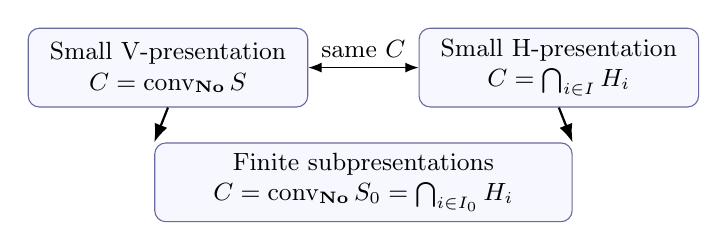
\begin{tikzpicture}[node distance=1.1cm,>=Latex,
 box/.style={draw=MidnightBlue!65,fill=blue!3,rounded corners,align=center,
 minimum width=3.55cm,minimum height=1cm,font=\small}]
\node[box] (v) {Small V-presentation\\$C=\conv_{\No}S$};
\node[box,right=1.4cm of v] (h) {Small H-presentation\\$C=\bigcap_{i\in I}H_i$};
\node[box,below=.95cm of $(v)!0.5!(h)$,minimum width=5.3cm] (p)
 {Finite subpresentations\\$C=\conv_{\No}S_0=\bigcap_{i\in I_0}H_i$};
\draw[->,thick] (v.south) -- (p.north west);
\draw[->,thick] (h.south) -- (p.north east);
\draw[<->] (v) -- node[above,font=\small]{same $C$} (h);
\end{tikzpicture}
\end{center}

\subsection{Definability is already a finiteness condition}
\begin{corollary}[Small hulls and definability]\label{poly:bf:cor:defV}
For a small hull $C=\VC S$, the following are equivalent:
\begin{enumerate}[label=(\roman*)]
\item $C$ is a finite polytope.
\item $C$ is ordered-field definable.
\item $C$ is an intersection of a set of ordered-field definable classes.
\end{enumerate}
In (iii), finite generators from the original $S$ already generate $C$.
\end{corollary}
\begin{proof}
Finite hulls are definable, and a definable class is a singleton-indexed
intersection. For (iii), the finite sandwich yields $C\subseteq\VC{S_0}$
for a finite $S_0\subseteq S$, while the reverse inclusion is automatic.
\end{proof}

\begin{corollary}[Definable small H-classes]\label{poly:bf:cor:defH}
If a small halfspace intersection $H$ is ordered-field definable, then a
finite subsystem of its original rows defines $H$. Hence it is a
polyhedron; if nonempty and bounded, it is a finite polytope.
\end{corollary}
\begin{proof}
If no finite subsystem sufficed, the type consisting of every row and the
single formula $x\notin H$ would be finitely satisfiable. Saturation would
contradict the definition of $H$. The remaining assertions are finite
polyhedral theory.
\end{proof}

These results have a useful interpretation. A small hull is a small
\emph{union} of definable finite hulls. If it is also a small
\emph{intersection} of definable classes, saturation forces finite
compression. This is a standard compactness mechanism with unusually
strong geometric consequences because all externally set-sized data are
small relative to the full surreal field.

\section{Polarity and the obstruction to vertex generation}\label{poly:bf:sec:polar}

For a convex class $P$ containing $0$, write
\[
 P^\circ=\{y\in\No^d:y\cdot x\le1\text{ for every }x\in P\}.
\]
If $P=\VC S$, testing the generators suffices, so $P^\circ$ has the small
H-presentation $y\cdot s\le1$ for $s\in S$.

\begin{theorem}[Small-hull polarity]\label{poly:bf:thm:polar}
Let $P=\VC S$ be full-dimensional and let $0\in\ri P$.
Then $P^\circ$ is closed, bounded, and has $0$ in its interior. Moreover,
\[
 P^{\circ\circ}=P,
 \qquad
 P^\circ\text{ is a small hull}
 \ \Longleftrightarrow\ P\text{ is a finite polytope}.
\]
\end{theorem}
\begin{proof}
Choose $M>0$ with $P\subseteq[-M,M]^d$. Then a sufficiently small box
around $0$, for example of radius $1/(2dM)$, lies in $P^\circ$.
Choose $r>0$ so small that each $\pm r e_j$ lies in $P$. Testing these
points gives $|y_j|\le1/r$ for $y\in P^\circ$, proving boundedness.
Closedness follows directly from the defining halfspaces.

The inclusion $P\subseteq P^{\circ\circ}$ is immediate. If $x\notin P$,
strong separation gives $u\cdot P\le c-1$ and $u\cdot x\ge c+1$.
Since $0\in P$, $c\ge1$. Hence $u/c\in P^\circ$, but
$(u/c)\cdot x>1$. This proves the reverse inclusion.

If $P^\circ$ is a small hull, it has both a small V- and a small
H-presentation. By \cref{poly:bf:thm:rigidity}, it is a finite polytope. Its finite
vertex list then gives a finite H-presentation of $P^{\circ\circ}=P$;
the original small V-presentation and rigidity make $P$ finite. Conversely,
the polar of a finite polytope containing $0$ in its interior is a bounded
finite polyhedron, hence a finite polytope.
\end{proof}

\begin{corollary}[A bounded small H-class is generated by its extreme
points only in the finite case]\label{poly:bf:cor:KM}
Let $H$ be a nonempty bounded small halfspace intersection. Then
\[
 H=\conv_{\No}(\ext H)
 \quad\Longleftrightarrow\quad H\text{ is a finite polytope}.
\]
The same equivalence holds when the hull on the left is replaced by its
order-box closure.
\end{corollary}
\begin{proof}
By \cref{poly:bf:cor:Hvertices}, $\ext H$ is a set. Equality would give a small
V-presentation and therefore a finite polytope. The converse is finite
polytope theory. By \cref{poly:bf:cor:closed}, the hull of the set $\ext H$ is
already closed, so taking its closure does not change it.
\end{proof}

This is not a contradiction to a real compact-convex generation theorem:
order boundedness and pointwise closedness in $\No^d$ supply neither its
compactness hypothesis nor its Archimedean setting. The failure is sharper
than merely requiring more vertices. In \cref{poly:bf:thm:polar}, a nonfinite
small hull has a polar that cannot be generated by \emph{any set} of
points, even points that are not extreme.

\section{Real faces and one-infinitesimal exposure}\label{poly:bf:sec:lex}

For a real convex set $C\subseteq\R^d$, define its
\emph{generator extension}
\[
 \upc C=\conv_{\No}C.
\]
The generators here are the actual real points of $C$. By
\cref{poly:bf:cor:basechange}, its faces are the classes $\upc F$ for real faces
$F$ of $C$; its affine dimension is unchanged. By \cref{poly:bf:thm:Vface}, all
these faces are exposed over $\No$.

\subsection{The classical invariant}
For a nonempty proper real face $F$ of $C$, let $r_C(F)$ be the minimum
length of a chain
\[
 C=F_0\supsetneq F_1\supsetneq\cdots\supsetneq F_r=F
\]
in which $F_j$ is an exposed face of $F_{j-1}$, using a real affine
functional on the latter's affine hull. Mart\'inez-Legaz proved that every
face admits such a chain, defined its degree of non-exposedness, and
established the bound~\cite{bf:martinez}
\[
 \delta_C(F)=r_C(F)-1
 \ \le\ \dim C-\dim F-1.
\]
Recent work studies the extension of face-characterization questions to
infinite-dimensional vector spaces~\cite{bf:gorokhovik}; that is a different
change of scope from the finite-dimensional, proper-class scalar setting
used here.

For completeness, the existence and dimension bound also follow by an
ordinary supporting-hyperplane argument. Choose $p\in\ri F$. Unless the
current convex set is $F$, the point $p$ lies on its relative boundary:
a face containing a relative interior point would be the entire set.
A real supporting hyperplane at $p$ cuts a proper exposed face containing
$F$. Continue in that face's affine hull. At every step the dimension
strictly decreases. A proper inclusion of nonempty faces cannot preserve
affine dimension, by \cref{poly:bf:lem:trace}; consequently the process reaches
$F$ after at most $\dim C-\dim F$ steps.

\subsection{An exact polynomial translation}
Fix a positive $\eps\in\No$ infinitesimal relative to $\R$: $0<\eps<r$
for every real $r>0$. A finite polynomial with real coefficients has the
sign of its first nonzero coefficient when evaluated at $\eps$. In
particular, $\eps$ is transcendental over $\R$.

\begin{definition}
Let $m_\eps(C,F)$ be the least $m\ge0$ for which there are real linear
functionals $u_0,\ldots,u_m$ such that
\[
 U_\eps=u_0+\eps u_1+\cdots+\eps^m u_m
\]
exposes $\upc F$ in $\upc C$. Functionals are considered on $\aff C$,
and may be extended to $\R^d$. A constant term in an affine functional is
absorbed by evaluating its difference from a fixed $p\in F$.
\end{definition}

\begin{theorem}[Polynomial degree equals classical non-exposedness]\label{poly:bf:thm:degree}
For every nonempty proper face $F$ of a real finite-dimensional convex set
$C$,
\[
 \boxed{m_\eps(C,F)=r_C(F)-1=\delta_C(F).}
\]
It is independent of the chosen positive real-infinitesimal $\eps$, and
\[
 0\le m_\eps(C,F)\le\dim C-\dim F-1.
\]
\end{theorem}
\begin{proof}
Choose a shortest exposed chain of length $r$, a point $p\in F$, and
real linear functionals $u_0,\ldots,u_{r-1}$ for its successive steps,
normalized only by subtracting their values at $p$. For a real point
$x\in C\setminus F$, let $j\in\{0,\ldots,r-1\}$ be the index with
$x\in F_j\setminus F_{j+1}$. Then $u_i(x-p)=0$ for $i<j$ and $u_j(x-p)<0$. The subsequent values can
have either sign, but the first nonzero real coefficient determines
\[
 U_\eps(x-p)=\sum_{i=0}^{r-1}\eps^i u_i(x-p)<0.
\]
It is zero for real $x\in F$. Finite surreal convex combinations preserve
nonpositivity. A combination has value zero only if every generator with
positive coefficient belongs to $F$. Thus $U_\eps$ exposes $\upc F$, and
$m_\eps(C,F)\le r-1$.

Conversely, suppose a polynomial of degree $m$ exposes $\upc F$.
For real $x\in C$, the coefficient vector
\[
 (u_0(x-p),u_1(x-p),\ldots,u_m(x-p))
\]
is lexicographically nonpositive, and it is zero precisely on $F$.
Indeed, a nonzero coefficient vector cannot evaluate to zero at the
transcendental $\eps$. Restrict successively to the zero sets of $u_0$,
then $u_1$, and so on. At each stage, the next functional is nonpositive
on the current face. Its zero set is therefore exposed there. Discard
stages at which the functional is constant on the current face. The
remaining chain reaches $F$ in at most $m+1$ strict steps, giving
$r_C(F)\le m+1$. The two bounds prove the formula.
\end{proof}

The new notation $m_\eps$ does not introduce a different real invariant.
The theorem identifies exactly what a one-infinitesimal polynomial
encoding measures. Its proof also explains why the coefficients must be
real, or belong to a specified field over which $\eps$ is infinitesimal.
Allowing arbitrary surreal coefficients would make the ``degree'' vacuous:
any surreal exposing normal could be placed in degree zero.

\noindent\wtag{} This is the report's third notion of degree. Part~I's
degree (\cref{poly:thm:degree}) is the least degree of a polynomial height
vector over a fixed real base; Part~VIII's (\cref{poly:cd:def:degree}) is
the homogeneous degree of a rational arc along which every vertex moves;
the degree here, $m_\eps(C,F)=\delta_C(F)$, is the degree of
non-exposedness of a real face.

\section{An explicit sharp family in every codimension}\label{poly:bf:sec:sharp}

We now construct compact real convex bodies for which the bound in
\cref{poly:bf:thm:degree} is attained. This supplies concrete test objects rather
than merely an abstract dimension estimate.

Set $K_1=[0,1]$. For $d\ge2$, write $x=(z,t)\in\R^{d-1}\times\R$ and set
\begin{align}
 G_d&=\{(z,\norm z_2^2):z\in\R^{d-1},\ \norm z_2\le1\},\\
 K_d&=\conv_\R\bigl((K_{d-1}\times\{0\})\cup G_d\bigr).
 \label{poly:bf:eq:Kd}
\end{align}
Each $K_d$ is compact: the union inside the hull is compact, and its convex
hull is the continuous image of a compact collection of at most $d+1$
points and their simplex of coefficients. It is full-dimensional because
$K_{d-1}\times\{0\}$ spans its base hyperplane and $G_d$ contains points
above that hyperplane. These real sets are also semialgebraic, by their
finite quantified descriptions and real quantifier elimination.

\begin{lemma}[A forced first exposure]\label{poly:bf:lem:forced}
The origin is an extreme point of $K_d$. Its only proper exposed face
containing it, for $d\ge2$, is $K_{d-1}\times\{0\}$.
\end{lemma}
\begin{proof}
Every last coordinate in \eqref{poly:bf:eq:Kd} is nonnegative, and a point of $G_d$
has last coordinate zero only at the origin. Thus
\[
 K_d\cap\{t=0\}=K_{d-1}\times\{0\}.
\]
Extremality of the origin follows inductively from extremality in this
base face.

Suppose a nonzero real linear functional $(a,b)\cdot(z,t)$ has its maximum
at $0$ on $K_d$. For any fixed $v\in\R^{d-1}$ and all sufficiently small
positive real $s$, both
\[
 s\,a\cdot v+b s^2\norm v_2^2\le0,
 \qquad
 -s\,a\cdot v+b s^2\norm v_2^2\le0
\]
hold. Dividing by $s$ and letting $s$ decrease through ordinary reals
forces $a\cdot v=0$. Hence $a=0$, and the nonzero supporting functional
has $b<0$. Its maximizing face is exactly the displayed base face.
\end{proof}

\begin{theorem}[Sharp degree and sharp depth]\label{poly:bf:thm:sharp}
For every $d\ge1$,
\[
 r_{K_d}(\{0\})=d,
 \qquad m_\eps(K_d,\{0\})=d-1.
\]
An exposing functional on $\upc {K_d}$ is
\[
 L_\eps(x_1,\ldots,x_d)
 =-x_d-\eps x_{d-1}-\cdots-\eps^{d-1}x_1.
\]
For every pair $d>f\ge0$, the product
\[
 C=K_{d-f}\times[-1,1]^f,
 \qquad F=\{0\}\times[-1,1]^f
\]
has $\dim C=d$, $\dim F=f$, and $m_\eps(C,F)=d-f-1$.
\end{theorem}
\begin{proof}
For $d=1$, the origin is exposed by $-x_1$, so the depth is $1$.
For $d\ge2$, \cref{poly:bf:lem:forced} forces the first step in every exposed
chain to be the base $K_{d-1}\times\{0\}$. Consequently the minimum depth
is one more than the depth in $K_{d-1}$, giving $d$ by induction.
The degree formula follows from \cref{poly:bf:thm:degree}. The displayed
functional is obtained by using the successive negative coordinate
functionals along the forced chain.

For the product, that same polynomial functional, ignoring the last $f$
coordinates, gives the upper bound. Any exposing polynomial for the
product face restricts on $K_{d-f}\times\{0\}$ to one exposing its origin.
It therefore has degree at least $d-f-1$, proving the lower bound.
\end{proof}

\begin{center}
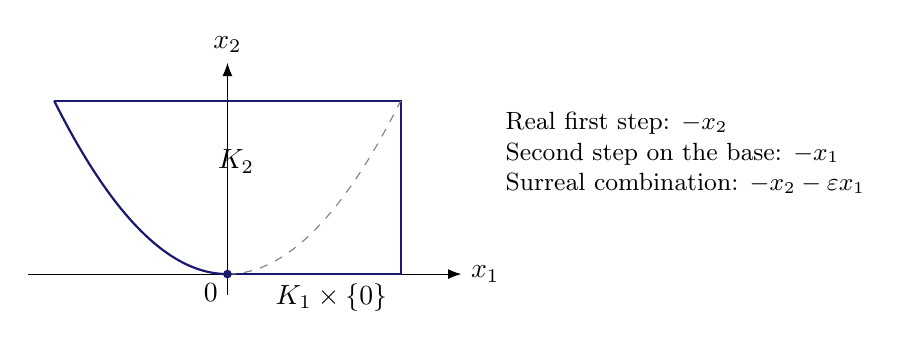
\begin{tikzpicture}[scale=2.2,>=Latex]
\draw[->] (-1.15,0)--(1.35,0) node[right]{$x_1$};
\draw[->] (0,-.12)--(0,1.22) node[above]{$x_2$};
\draw[thick,MidnightBlue,domain=-1:0,samples=70] plot (\x,{\x*\x});
\draw[thick,MidnightBlue] (0,0)--(1,0)--(1,1)--(-1,1);
\draw[dashed,black!50,domain=0:1,samples=60] plot (\x,{\x*\x});
\fill[MidnightBlue] (0,0) circle (.025);
\node[below left] at (0,0){$0$};
\node[below] at (.6,0){$K_1\times\{0\}$};
\node at (.05,.65){$K_2$};
\node[align=left,font=\small,anchor=west] at (1.55,.7)
 {Real first step: $-x_2$\\Second step on the base: $-x_1$\\
 Surreal combination: $-x_2-\eps x_1$};
\end{tikzpicture}
\end{center}

\subsection{The necessary semantic distinction}
\needspace{8\baselineskip}
\begin{important}{Generator extension is not definable extension}
For a semialgebraic real set $C$, the two classes
\[
 \upc C=\conv_{\No}(C(\R))\qquad\text{and}\qquad C(\No)
\]
are generally different. The second means evaluating a defining
semialgebraic formula with arbitrary surreal variables. The first retains
only the real points as generators. The exposure theorems in
Sections~\ref{poly:bf:sec:lex}--\ref{poly:bf:sec:sharp} concern the first.
\end{important}

The sharp family gives an exact witness. For $d\ge2$, the full
semialgebraic extension of its paraboloid contains the point with
\[
 x_{d-1}=-\eps/2,\qquad x_d=\eps^2/4,
 \qquad x_j=0\quad(j<d-1).
\]
At this point,
\[
 L_\eps(x)=-\eps^2/4+\eps^2/2=\eps^2/4>0.
\]
Thus $L_\eps$ does \emph{not} support $K_d(\No)$ at the origin. Since it
is nonpositive on $\upc {K_d}$, the displayed point is not in that
set-generated hull. This explicitly prevents the erroneous conclusion
that all faces of every semialgebraic surreal convex body are exposed.

\section{The rational moment curve: a complete face classification}\label{poly:bf:sec:moment}

The next example exhibits genuinely infinite combinatorics. Fix $d\ge2$
and define
\[
 m_d(t)=(t,t^2,\ldots,t^d),\qquad
 M_d=\conv_{\No}\{m_d(t):t\in\Q\},\qquad
 k=\lfloor d/2\rfloor.
\]
Although the rational curve is unbounded in real Euclidean space, all its
coordinates are finite reals. Hence $M_d\subseteq[-\omega,\omega]^d$.
It is closed by \cref{poly:bf:cor:closed} and has full affine dimension by the
Vandermonde determinant.

\begin{theorem}[All faces of the rational moment hull]\label{poly:bf:thm:moment}
The nonempty proper faces of $M_d$ are exactly
\[
 F_A=\conv_{\No}\{m_d(a):a\in A\},
 \qquad A\subseteq\Q,
 \qquad 1\le |A|\le\lfloor d/2\rfloor.
\]
Each $F_A$ is an $(|A|-1)$-simplex. Every rational curve point is an extreme
point. There is no set-sized halfspace presentation of $M_d$.
\end{theorem}
\begin{proof}
First, let $A$ have at most $k$ elements. The real polynomial
\[
 q_A(t)=\prod_{a\in A}(t-a)^2
\]
has degree at most $d$, is nonnegative on $\R$, and vanishes exactly at
$A$. Express it as $q_A(t)=c-u\cdot m_d(t)$, allowing zero coefficients
through degree $d$. This affine slack is nonnegative at all generators,
and zero exactly at the generators indexed by $A$. It exposes $F_A$.
Vandermonde determinants show that any at most $d+1$ distinct moment
points are affinely independent, so $F_A$ is the indicated simplex.

Conversely, let $F$ be a nonempty proper face. By \cref{poly:bf:thm:Vface}, it is
exposed by a surreal affine functional, with nonzero slack polynomial
\[
 q(t)=c-u\cdot m_d(t)\in\No[t],\qquad \deg q\le d,
 \qquad q(t)\ge0\quad(t\in\Q).
\]
The polynomial is nonzero because a zero polynomial would give zero slack
on all generators, hence the entire hull as the face. Put
$B=\max_j|q_j|>0$, where $q_j$ are its finitely many coefficients, including
the constant coefficient. All coefficients of $q/B$ are finite surreals,
and at least one is exactly $1$ or $-1$. Take their real standard parts to
obtain a nonzero polynomial $\bar q\in\R[t]$ of degree at most $d$.
Standard part exists for a finite surreal by the real cut it determines;
it preserves sums, products, and weak inequalities among finite elements.

For rational $t$, $\bar q(t)=\st(q(t)/B)\ge0$. Real continuity and the
density of $\Q$ imply $\bar q\ge0$ throughout $\R$. Every rational zero
of $q$ is a zero of $\bar q$. A nonzero real polynomial nonnegative on all
of $\R$ has even multiplicity at each distinct real root. Therefore the
set of rational zeros of $q$ has at most $\lfloor d/2\rfloor$ elements.
By \cref{poly:bf:lem:trace}, these are exactly the parameters generating $F$.

Singleton choices of $A$ prove that all rational curve points are extreme.
There are infinitely many of them. A set-sized H-presentation would make
$M_d$ a finite polytope by \cref{poly:bf:thm:rigidity}, contradicting its infinitely
many extreme points.
\end{proof}

The last argument can also be read as a classification of the real
finite-convex-combination hull of the rational moment curve, transported
to $\No$ by \cref{poly:bf:cor:basechange}. Its special surreal feature is that this
hull becomes order bounded and closed without gaining the extra face
strata that a usual real compactification would introduce.

\subsection{The resulting face poset}
Including the empty face and the top element, its abstract face poset is
\[
 \{\varnothing\}\ \cup\
 \{A\subseteq\Q:1\le|A|\le k\}\ \cup\ \{\top\},
\]
ordered by inclusion among the finite subsets, with $\top$ above all.
Thus every collection of at most $k$ vertices spans a face, but there are
no other proper faces.

\begin{center}
\begin{tabular}{@{}cll@{}}
\toprule
Dimension & Nonempty proper face dimensions & Example of missing faces\\
\midrule
$2,3$ & $0$ only & No edges\\
$4,5$ & $0,1$ & No two-dimensional faces\\
$6,7$ & $0,1,2$ & No three-dimensional faces\\
$d$ & $0,\ldots,\lfloor d/2\rfloor-1$ & No facets\\
\bottomrule
\end{tabular}
\end{center}

This is not a finite-polytope face lattice, and ordinary gradedness by
geometric dimension fails at its top element. Every finite subhull is an
ordinary polytope, but a face of a finite subhull need not remain a face
when more rational generators are admitted. The passage to the directed
union of finite hulls is exactly where finite polytope intuition ceases
to determine the global face structure.

\subsection{The polar has a complementary face-dimension gap}
The polar can be classified just as explicitly. Choose
\[
 b=\frac{1}{d+1}\sum_{r=0}^{d}m_d(r),\qquad P_d=M_d-b,
\]
and set
\[
 H_d=P_d^\circ
 =\{y\in\No^d:y\cdot(m_d(t)-b)\le1\text{ for every }t\in\Q\}.
\]
The barycenter $b$ lies in the interior of the full-dimensional simplex
on $m_d(0),\ldots,m_d(d)$, so $0\in\operatorname{int}P_d$.
Both $P_d$ and $H_d$ are closed, bounded, and full-dimensional.

\begin{theorem}[Complete dual classification; no vertices in the polar]
\label{poly:bf:thm:momentpolar}
The nonempty proper faces of $H_d$ are exactly
\[
 G_A=\{y\in H_d:y\cdot(m_d(a)-b)=1\text{ for every }a\in A\},
 \quad 1\le |A|\le k,
\]
where $A$ ranges over finite subsets of $\Q$ and $k=\lfloor d/2\rfloor$.
They satisfy
\[
 \dim G_A=d-|A|,\qquad
 G_A\subseteq G_B\ \Longleftrightarrow\ B\subseteq A.
\]
In particular, $H_d$ has no nonempty faces of dimension less than
$\lceil d/2\rceil$, and has no extreme points. The correspondence
$F_A-b\leftrightarrow G_A$, together with the interchange of the empty
and full faces, is an order-reversing bijection of the two face posets.
For corresponding proper faces the dimensions sum to $d-1$.
\end{theorem}
\begin{proof}
At $y\in H_d$, its active parameters are those $t\in\Q$ with
$y\cdot(m_d(t)-b)=1$. If this set is nonempty, it is the trace of a
nonempty proper exposed face of $P_d$. The classification in
\cref{poly:bf:thm:moment} makes it a set $A$ of at most $k$ parameters.

Its active row vectors are linearly independent. Indeed, if
$\sum_{a\in A}\lambda_a(m_d(a)-b)=0$, taking the scalar product with $y$
gives $\sum_a\lambda_a=0$. Hence $\sum_a\lambda_a m_d(a)=0$ is an affine
dependence among at most $k$ distinct moment points. Vandermonde
independence forces every $\lambda_a=0$. The active-face theorem therefore
makes the minimal face at $y$ equal to $G_A$, of dimension $d-|A|$.
Every nonempty proper face has a relative interior point, so this accounts
for all possibilities.

It remains to prove that every listed $A$ actually occurs, without
additional active parameters. Write
$q_A(t)=c_A-u_A\cdot m_d(t)$ for the square-product polynomial from the
previous theorem, and put
\[
 \alpha_A=c_A-u_A\cdot b
 =\frac{1}{d+1}\sum_{r=0}^{d}q_A(r)>0.
\]
The strict inequality holds because $q_A\ge0$ and $A$ cannot contain all
$d+1$ distinct parameters $0,\ldots,d$. For $y_A=u_A/\alpha_A$,
\[
 1-y_A\cdot(m_d(t)-b)=q_A(t)/\alpha_A\ge0
\]
for all rational $t$, with equality exactly on $A$. Thus $y_A\in H_d$
has precisely the required active set. The preceding rank calculation
and active-face theorem prove its face dimension.

If $B\subseteq A$, the equations give $G_A\subseteq G_B$. Conversely,
such an inclusion puts $y_A$ in $G_B$, so its exact active set implies
$B\subseteq A$. This proves both distinctness and the asserted order
relation. Since $d-|A|\ge d-k=\lceil d/2\rceil\ge1$, there are no
zero-dimensional faces. The full dual correspondence and the dimension
identity follow from the two classifications.
\end{proof}

\begin{center}
\begin{tabular}{@{}cll@{}}
\toprule
Dimension & Proper face dimensions of $P_d$ & Proper face dimensions of $H_d$\\
\midrule
$2$ & $0$ & $1$\\
$3$ & $0$ & $2$\\
$4$ & $0,1$ & $2,3$\\
$5$ & $0,1$ & $3,4$\\
$6$ & $0,1,2$ & $3,4,5$\\
\bottomrule
\end{tabular}
\end{center}

Thus this is an explicit mutually polar pair with dual face posets and
all proper faces exposed, but with no facets on one side and no vertices
on the other. Each minimal nonempty face on the H-side is still
positive-dimensional. It has no nonempty proper face of its own, because
faces of faces are faces of the ambient convex class. By
\cref{poly:bf:thm:polar}, $H_d$ is not the convex hull of any set of points.

\section{One-dimensional examples and failure modes}\label{poly:bf:sec:examples}

\subsection{A closed bounded hull with no minimum}
Let
\[
 C=\conv_{\No}\{1/n:n\ge1\}
   =\bigcup_{n\ge1}[1/n,1].
\]
The equality follows because every finite convex combination lies between
its smallest generator and $1$, and every interval on the right is
already a two-generator hull. This class is closed and bounded by
\cref{poly:bf:cor:closed}. It has maximum $1$ but no minimum: if $x\ge1/n$, then
$1/(n+1)<x$ is another element. Its only nonempty proper face is $\{1\}$.
It is not a finite polytope, hence has no small H-presentation.

There is a direct cut proof of the last assertion. A nontrivial halfspace
in one dimension is either a lower bound $x\ge a$ or an upper bound
$x\le b$. Validity on $C$ forces $b\ge1$, and it forces
$a<1/n$ for every $n$; equality for some $n$ would fail at $1/(n+1)$.
Given any set of such lower bounds, the cut property supplies
\[
 a<z<1/n\quad\text{for every listed }a\text{ and every }n,
 \qquad z>0.
\]
This $z$ satisfies all listed halfspaces but is not in $C$.

There is nevertheless a proper-class H-presentation:
\[
 C=\{x:x\le1,\ x\ge\eta\text{ for every positive real-infinitesimal }
 \eta\in\No\}.
\]
Every member of $C$ exceeds all positive infinitesimals. Conversely, a
positive infinitesimal $x$ violates the inequality indexed by $2x$; a
nonpositive $x$ violates any positive one. This is a transparent example
of why the word ``set'' cannot be omitted from the rigidity theorem.

\subsection{A countable bounded H-system with no vertices}
Consider
\[
 H=\bigcap_{n\ge1}[-1-1/n,\,1+1/n].
\]
It contains $[-1,1]$ and is bounded by $[-2,2]$. Every defining inequality
is strict at every feasible point: equality in a row indexed by $n$ would
violate the tighter row indexed by $n+1$. Thus no point has an active
nonzero row. The active-face theorem shows that every point is an
interior point and that $H$ has no extreme points. It is closed as an
intersection of closed intervals. Hence this nonempty bounded class is
simultaneously open and closed in the order-box sense.

One can see the local neighborhood directly. At a point $x\in H$, all
row slacks are positive, and a positive surreal smaller than every slack
allows both $x+\delta$ and $x-\delta$ to stay feasible. No finite subsystem
defines $H$: a finite list allows one of its outer endpoints, whereas the
full list excludes that endpoint. It follows either directly or by
\cref{poly:bf:thm:rigidity} that $H$ is not a small hull.

\subsection{The finite surreals as a hull}
Another simple example is
\[
 \conv_{\No}\R
 =\mathcal O
 :=\{x\in\No:|x|<r\text{ for some real }r>0\}.
\]
Every finite combination of real endpoints is finite, and every finite
surreal lies between two reals. The class $\mathcal O$ is a small hull,
closed and bounded by $\omega$, but has no extreme points. It cannot be a
small halfspace intersection. This example shows that small V-classes
need not be generated by their extreme points either; the general face
exposure theorem asserts exposure of \emph{existing} faces, not their
existence or sufficiency for generation.

\subsection{Why finite real approximation is not enough}
A positive real number substituted for $\eps$ in the sharp examples need
not expose the intended face: real points can have first-stage slack
smaller than that fixed perturbation scale. Likewise, no finite list of
rows in the countable interval example captures all its infinitesimal
boundary information. Exact finite checks are useful for finding algebraic
errors, but the small-cut or saturation step is logically indispensable.

\section{Cardinal versions and the precise role of the universe}\label{poly:bf:sec:cardinal}

The proofs use no multiplication peculiar to Conway normal forms. They
apply to a more general saturated real closed field whenever the
presentations fit below its saturation threshold.

\begin{theorem}[Set-sized saturated-field version]\label{poly:bf:thm:kappa}
Let $K$ be a $\kappa$-saturated real closed ordered field, where
$\kappa$ is uncountable. Replace ``set'' in
\cref{poly:bf:thm:separate,poly:bf:thm:Vface,poly:bf:thm:certificates,poly:bf:thm:active,poly:bf:thm:sandwich,poly:bf:thm:rigidity}
by ``of cardinality less than $\kappa$,'' including all parameter families.
The resulting statements hold over $K$.
\end{theorem}
\begin{proof}
Every type used in the proofs has fewer than $\kappa$ formulas and
parameters. Taking all finite subsets of a family of size less than
$\kappa$ still yields fewer than $\kappa$ many subsets when the family is
infinite; finite families cause no issue. Only finite unions of parameter
families are needed. Use $\kappa$-saturation in place of
\cref{poly:bf:thm:saturation}. Uniform local radii are obtained from the same
small positive-bound types.
\end{proof}

In particular, no regularity assumption on $\kappa$ is needed for these
finite-union cardinal estimates. The full surreal case is the external
version in which every set-sized family is admissible.

\begin{proposition}[One-dimensional geometry detects cuts]\label{poly:bf:prop:cuts}
Let $K$ be an ordered field and $\kappa$ an uncountable cardinal.
The following are equivalent:
\begin{enumerate}[label=(\roman*)]
\item Every cut $L<R$ with $|L\cup R|<\kappa$ has a strict interpolant,
including cuts with an empty side.
\item Every subset of $K$ of size less than $\kappa$ is order bounded, and
any two disjoint hulls of nonempty such subsets in dimension one have a
strict affine separator.
\end{enumerate}
If $K$ is real closed, these conditions also imply realization of every
finitely satisfiable partial type with fewer than $\kappa$ formulas and
parameters in finitely many variables. Thus they give all the geometric
conclusions of \cref{poly:bf:thm:kappa}.
\end{proposition}
\begin{proof}
For (i)$\Rightarrow$(ii), use cuts with an empty side to obtain bounds.
Two disjoint nonempty convex subsets of a line are ordered one wholly
before the other. After interchanging the generators if necessary, the
corresponding cut $S<T$ therefore has an interpolant, which is a strict
separator.

For (ii)$\Rightarrow$(i), when both $L,R$ are nonempty their convex hulls
are disjoint, and a strict affine separator gives a point strictly between
all elements of $L$ and all elements of $R$. If a side is empty, use the
assumed bound, enlarging a weak bound by $1$ when necessary.

For the real closed assertion, put the parameters in a real closed
subfield $K_0\subseteq K$ of size less than $\kappa$. Quantifier elimination
and compactness, followed by downward L\"owenheim--Skolem, give a realizing
real closed extension $E/K_0$ of size less than $\kappa$. The relative
embedding proof of \cref{poly:bf:lem:embedding} embeds $E$ into $K$ over $K_0$:
all intermediate fields and cuts have size bounded by
$\max(|K_0|,|E|,\aleph_0)<\kappa$. This realizes the type in $K$.
\end{proof}

Thus an omitted small cut in an old field is already an obstruction to
one-dimensional uniform separation. This is the elementary geometric
link to the repository's across-universes program~\cite{bf:repouniv}. No
particular forcing or gap-spectrum assertion from that report is required
for this implication.

\section{Proof review, exact checks, and a formalization route}\label{poly:bf:sec:verification}

\subsection{Dependency structure}
There are three independent proof streams.
\begin{center}
\small
\begin{tabular}{@{}>{\raggedright\arraybackslash}p{.25\textwidth}>{\raggedright\arraybackslash}p{.67\textwidth}@{}}
\toprule
Input & Consequences\\
\midrule
Cuts + real closedness + compactness & Small-type realization; strong
separation; all small-hull faces exposed; finite implication certificates;
finite sandwiches and V/H rigidity.\\[4pt]
Positive small lower bounds + finite linear algebra & Uniform neighborhoods
in active affine spaces; finite active-face descriptions; the set of
vertices of a small H-class.\\[4pt]
Real facial chains + infinitesimal sign rule & Exact polynomial degree;
recursive sharp compact bodies; explicit distinction between generator
extension and definable extension.\\
\bottomrule
\end{tabular}
\end{center}
The moment-curve classification combines exposure, a coefficientwise
standard-part argument, elementary polynomial root multiplicity, and
Vandermonde independence. Polarity uses separation and finite-description
rigidity, not any unproved compactness principle.

The most sensitive checks are the set-sized nature of each type, the
restriction of the unit exposure margin to generators, the fact that the
hulls themselves can be proper classes, and the distinction between
$\upc C$ and $C(\No)$. The proofs explicitly address all four.

\subsection{What the supplied code checks}
The package contains a standard-library Python program using exact
rational arithmetic (\wtag{} shipped as \pathcode{code/13-beyond-finite-verify.py}). It checks square-product moment polynomials,
affine Vandermonde determinants, the leading coefficient signs of sampled
recursive sharp-family generators, the identity $\eps^2/4$ in the
definable-extension counterexample, the exact active normals and ranks in the polar classification, and
finite nonnegative row-combination certificates. The recorded results can be reproduced with
\begin{verbatim}
python3 code/13-beyond-finite-verify.py \
    --output /path/to/scratch/verification_results.json
\end{verbatim}
(\wtag{} Source~13 printed \texttt{python3 code/verify.py --output}
\pathcode{data/verification_results.json}. The program writes a file only when
\texttt{--output} is given; pass a path outside the report directory, as
above, so that the shipped record
\pathcode{data/13-beyond-finite-verification_results.json} (console output
\pathcode{data/13-beyond-finite-verification_stdout.txt}) is never
overwritten. The shipped \pathcode{code/13-beyond-finite-Makefile} still
names \texttt{code/verify.py}, \texttt{data/verification\_results.json} and
\texttt{article.tex}.)
These are finite regression checks, not evidence of model-theoretic
compactness, not a numerical implementation of the entire surreal field,
and not a replacement for any proof. In particular, a loop over rational
samples does not establish the moment-curve face classification; its
upper bound is the standard-part and even-multiplicity argument.

\subsection{A practical Lean decomposition}
\noindent\wtag{} This subsection is a proposal: nothing of this Part
is formalized. At the write phase no repository-authored Lean file of
\repo{} mentions Farkas duality, so its first layer has no counterpart in
the repository either.

A formalization should separate abstract finite-dimensional convexity from
the implementation of the surreal field. The first layer needs affine
faces, finite hull membership, finite exposure, and ordered-field Farkas
certificates. Existing ordered-field duality work provides a relevant
reference point~\cite{bf:dvorak}, but this manuscript has not verified that
its exact declarations are already present in the repository.

The second layer should take a \emph{saturation interface} as a hypothesis:
every suitably small finitely satisfiable family of formulas in finite
coordinate types has a realization. Under this interface, the sandwich
proof is short and reusable. The active-face theorem can be formalized
under the weaker interface providing a positive number below a small
family of positive numbers.

Only the third layer should instantiate these interfaces for a
universe-indexed surreal construction. In Lean, a proper class is not an
ordinary type inside the same universe; the smallness relationship must
be expressed with universes and lifting. A theorem about a fixed small
surreal type must not be silently advertised as saturation for every set
of that same universe. That foundational bookkeeping is a substantive
part of the proposed implementation, not a notation change.

Finally, the sharp-family and moment-curve arguments are separable
algebraic targets. Finite polynomial sign-at-infinitesimal lemmas,
coefficientwise standard part, and Vandermonde determinants can be
formalized before the full saturation theorem. No Lean file is supplied
here because no corresponding compilation was performed; a plausible
uncompiled script would not constitute verification.

\section{Further research questions}\label{poly:bf:sec:questions}

The following are proposed research directions, not claims that each is a
previously published open problem. The theorems above supply constraints
that a successful answer must respect.

\begin{question}[Birthdays and explicit separators]
Given a set of generators with a bound on their birthdays and a description
of a facial trace, what bounds can be proved for the birthday of an
exposing normal? Can a finite-complexity trace yield a normal with a
specified normal-form support or a controlled number of scales?
\end{question}
The general saturation proof is existential. It does not imply effective
extraction from an arbitrary presentation. A useful first target is a
countable family of generators given by polynomial or rational maps with
real coefficients and a semialgebraically described trace.

\begin{question}[Exact presentation thresholds in set-sized fields]
For a $\kappa$-saturated real closed field $K$, how small can an
H-presentation of a nonpolyhedral hull of fewer than $\kappa$ generators
be? Can the lower bound $\kappa$ forced by rigidity be attained, and which
cut cofinalities determine the exact minimum?
\end{question}
The one-dimensional cut examples suggest that different ordered fields
with the same elementary theory may have different exact presentation
spectra. Any proposed answer should separate the number of generators,
the number of rows, and the size of the parameter field.

\begin{question}[Polars beyond small generation]
For a bounded small H-class, characterize the points missing from the hull
of its extreme points. Can one describe them intrinsically by types,
active-row limits, or cuts in normal directions? What additional class-sized
data recover the full polar of a small V-class?
\end{question}
The rational moment-curve polar gives a concrete nonfinite family for
which any set of proposed generators must fail. A satisfactory description
must do more than enumerate additional vertices.

\begin{question}[Computation of exposure depth]
For real semialgebraic $C$ and a specified face $F$, what is the complexity
of computing the classical degree $\delta_C(F)$ and a shortest exposing
chain? Can this be turned into a symbolic certificate of minimal
infinitesimal polynomial degree?
\end{question}
The family $K_d$ gives a test with a provably forced first step at every
stage. It would be useful to find similarly transparent families with
prescribed branching in their shortest exposed chains, or with much
smaller semialgebraic descriptions at the same depth.

\begin{question}[Infinite face-poset realization]
Which set-sized posets occur as face lattices of small hulls in fixed
finite-dimensional surreal space? How can one characterize the additional
constraints beyond finite facial compatibility and an affine-dimension
bound?
\end{question}
The rational moment hull realizes a full finite-subset skeleton followed
by a dimension jump to the top. It shows that the gradedness and facet
structure of finite polytopes are not automatic. A systematic theory
should encode how faces of finite subhulls disappear under enlargement.

\begin{question}[Ground fields for exposing coefficients]
For $S\subseteq K^d$ in a proper ordered subfield $K\subseteq\No$, determine
when every facial trace can be exposed using finitely many infinitesimal
scales with coefficients in $K$. What field extension is minimally needed
when this fails?
\end{question}
For $K=\R$, the exact answer for generator extensions is controlled by
classical exposure depth. For general $K$, missing cuts can obstruct the
supporting-hyperplane constructions used in the real proof, even though
the full surreal exposing normal still exists by saturation.

\begin{question}[Completion choices]
Which explicitly defined enlargements of finite-combination hulls admit a
useful V/H duality beyond finite polytopes? Possibilities include specified
summable combinations or intersections indexed by controlled proper
classes. Which choices preserve a bipolar theorem and a tractable face
notion?
\end{question}
The rigidity theorem rules out obtaining a genuinely broader duality while
simultaneously retaining both set-sized presentations and only finite
convex combinations. At least one of those conditions has to change.

\begin{question}[A checked abstract compactness library]
Can the finite-sandwich, finite-consequence, and active-face arguments be
formalized once for saturated ordered fields and then instantiated for
surreal models, nonstandard real fields, and relevant universe-relative
subfields with explicit size hypotheses?
\end{question}
This is a focused integration target for \repo. It would connect the
repository's field foundations and across-universe questions to a
geometric API without requiring a general theory of proper-class
topological compactness.

\section{Conclusion}
The most important distinction in this geometry is not finite versus
infinite coordinates. It is the distinction between a finite presentation,
a set-sized presentation, and a proper-class presentation. In the full
surreal field, saturation makes a set-sized family of generators behave
as if every needed strict gap could be chosen simultaneously. That gives
closedness and strong exposure. On the inequality side it makes local
boundaries finitely active and every valid linear consequence finitely
certified. When the two sorts of presentation describe the same class,
the finite-sandwich theorem forces them both to collapse to finite ones.

The examples show that this is a structural boundary, not a vacuous
rephrasing of finite polytope theory. Countably generated hulls can have
infinitely many exposed vertices and no facets. Countably presented
bounded H-classes can have no vertices. Polarity can take a hull with a
countable list of generators to a class that no set can generate.
Infinitesimal functionals can expose every old real face while failing on
the full semialgebraic extension of the very same real body.

The proofs establish these statements under explicit hypotheses. Their
formal verification, effective refinements, and full priority assessment
remain separate tasks. They provide a concrete research program with
sharp obstructions and exact examples, rather than an unsupported claim
that changing the scalar field resolves a classical open conjecture.

\section{Notation and scope reference (Appendix~A of source~13)}\label{poly:bf:app:notation}
\begin{longtable}{@{}>{\raggedright\arraybackslash}p{.24\textwidth}>{\raggedright\arraybackslash}p{.68\textwidth}@{}}
\toprule
Notation or phrase & Meaning\\
\midrule
\endhead
$\No$ & The full surreal ordered field of the fixed current universe.\\[4pt]
Small & Indexed by an external set; in \cref{poly:bf:thm:kappa}, of size
less than $\kappa$.\\[4pt]
$d$ & Ordinary finite dimension, never a surreal integer.\\[4pt]
$\VC S$ & Finite-convex-combination hull with arbitrary surreal
coefficients. The generator family $S$ is a set.\\[4pt]
Small H-class & An intersection of a set of closed affine surreal
halfspaces. The feasible class need not be a set.\\[4pt]
Polytope & Convex hull of an ordinary finite list of points.\\[4pt]
Closed & Every exterior point has a disjoint positive-radius order box.\\[4pt]
Bounded & Contained in a box of some surreal radius; not necessarily
bounded by a real radius.\\[4pt]
$\upc C$ & Generator extension $\conv_{\No}(C(\R))$ of a real convex set.\\[4pt]
$C(\No)$ & Extension by a semialgebraic formula, when one is specified;
generally different from $\upc C$.\\[4pt]
$\delta_C(F)$ & Mart\'inez-Legaz's degree of non-exposedness of a real face.\\[4pt]
$m_\eps(C,F)$ & Minimum degree of an exposing polynomial in $\eps$ with
real linear-functional coefficients.\\[4pt]
$M_d$ & Hull of the moment curve at all rational parameters; not a
finite cyclic polytope.\\
\bottomrule
\end{longtable}

\section{Provenance and proof-status statement (Appendix~B of source~13)}\label{poly:bf:app:provenance}
The repository was consulted through its connected GitHub interface on
30 September 2026. Search results were pinned to commit
\begin{center}
\texttt{6996fee43cc97b6c16351def7507d59a95bf62f0}.
\end{center}
The two principal README files were fetched from the default branch on
that date. Their returned blob hashes were, respectively,
\begin{center}\small
\texttt{cf63fc5ff9ca9d8877e90f8e69ec34e6ded19d23},\\
\texttt{bfb819fc0cff4c42961a2048d21845af5a9522fd}.
\end{center}
The package's source notes (\wtag{} \pathcode{13-beyond-finite-SOURCES_AND_SCOPE.md}) distinguish that indexed commit from the
individual returned blobs; they do not assert that all fetched files were
read at a simultaneously pinned checkout.

\noindent\wtag{} Re-verified at the write phase: these are the blob hashes
of \pathcode{Algebra/SurrealNumbers/README.md} and
\pathcode{Algebra/SurrealNumbers/docs/foundations-and-computation/surreal-fields-across-universes/README.md},
both at commit \pathcode{6996fee43} and at \texttt{HEAD}
\pathcode{4e128356d}; the second README still states that nothing in that
report is formalized or Lean-verified.

The manuscript is AI-assisted and unrefereed. It contains complete written
proofs of its principal claims. It does not contain a proof-assistant
certificate, and its Python checks are explicitly finite algebraic
regressions. The original 1997 paper was consulted directly to establish
that lexicographical exposure, degree of non-exposedness, and the
codimension bound are prior results. No source or quotation is used as a
substitute for the proofs of the finite-description and surreal
consequences developed here.

\clearpage
\part*{Provenance and references}
\addcontentsline{toc}{part}{Provenance and references}

\appendix
\section{Provenance of the report}\label{poly:app:provenance}

\noindent\wtag{} This appendix was written in the merge.

\subsection{Sources}

The report was built in the batch-58 write phase from six manuscripts,
all dated 30~September 2026 and delivered on that day in six archives
(arrival commit \texttt{b2b626d}); they were placed in commit
\texttt{b30441a}, which staged manuscript~05's \nolinkurl{article.tex} and
\nolinkurl{README.md} as delivered and every other staged file under its
manuscript's prefix. Manuscripts are numbered by arrival within the batch
(manuscript~01, on a Keller map, went to another report).

{\small
\begin{longtable}{@{}>{\raggedright\arraybackslash}p{0.05\linewidth}>{\raggedright\arraybackslash}p{0.33\linewidth}>{\raggedright\arraybackslash}p{0.24\linewidth}>{\raggedright\arraybackslash}p{0.09\linewidth}>{\raggedright\arraybackslash}p{0.17\linewidth}@{}}
\toprule
No. & Title (archive; main file) & Delivered PDF, author line & Pin & Printed as\\
\midrule
\endhead
\bottomrule
\endfoot
05 & \emph{Finite-Scale Geometry of Surreal Liftings} (\nolinkurl{surreal_liftings_research.zip}; \nolinkurl{surreal_liftings/article.tex}) & 25~pp.\ A4; research manuscript prepared for Vladimir Reshetnikov, an AI-assisted contribution to the \repo{} research program & \texttt{5e0f4e0} & \cref{poly:part:lift}, base (whole)\\
02 & \emph{Surreal Polytopes at Finite and Transfinite Scales} (\nolinkurl{surreal_polytopes_research.zip}; \nolinkurl{surreal_polytopes/article.tex}) & 28~pp.\ Letter; research article prepared for Vladimir Reshetnikov & \texttt{6996fee} & \cref{poly:part:lift} (merged) and \cref{poly:part:ts}\\
06 & \emph{Surreal Polytopes: Affine Residues, Mixed-Volume Scales, and Simultaneous Segment Models} (\nolinkurl{Surreal_Polytopes_Research_Package.zip}; \nolinkurl{Surreal_Polytopes/article.tex}) & 27~pp.\ A4; research article prepared for Vladimir Reshetnikov & \texttt{6996fee} & \cref{poly:part:mv} (whole)\\
03 & \emph{Infinitesimal Boundary Geometry of Surreal Polytopes: Lexicographic traces, one-parameter descent, and Ehrhart universality} (\nolinkurl{surreal_polytope_research.zip}; \nolinkurl{surreal_polytopes/surreal_polytopes.tex}) & 28~pp.\ Letter; research manuscript prepared for Vladimir Reshetnikov & \texttt{6996fee} & \cref{poly:part:ehr} (whole)\\
07 & \emph{Invisible Complexity in Surreal Polytopes: Explicit polygons with identical all-order jets and identical initial slack matrices} (\nolinkurl{surreal_polytopes.zip}; \nolinkurl{surreal_polytopes/surreal_polytopes.tex}) & 26~pp.\ A4; research manuscript prepared for Vladimir Reshetnikov & \texttt{6996fee} & \cref{poly:part:ic}, base (whole)\\
04 & \emph{Beyond-All-Orders Extension Complexity in Surreal Polygon Geometry: Flat deformations, classical face lattices, and a sharp-order complexity gap} (\nolinkurl{surreal_polytopes_beyond_all_orders.zip}; \nolinkurl{surreal_polytopes_beyond_all_orders/article.tex}) & 26~pp.\ A4; research manuscript prepared for Vladimir Reshetnikov, developed with ChatGPT; independent review and formalization pending & \texttt{6996fee} & \cref{poly:part:ic} (merged)\\
\end{longtable}
}

The pin \texttt{6996fee} is commit
\texttt{6996fee43cc97b6c16351def7507d59a95bf62f0} (30~September 2026,
16:07:39~UTC); \texttt{5e0f4e0} is
\texttt{5e0f4e05046bacda3c6ba2643f19b91aa632436b}, its second parent.
Archives 02, 03 and 07 all wrap an inner directory named
\nolinkurl{surreal_polytopes/}; they are different packages.

\subsection{What each manuscript contributed}

\paragraph{Manuscript 05 (base; Part I).} The frame of Part~I: the affine
gauge and dependence space, the simultaneous leading-term compression
(\cref{poly:thm:pivot,poly:cor:height}), the flag classification
(\cref{poly:thm:flag}), the exact germ degrees
(\cref{poly:thm:degree,poly:thm:shadowdegree}) and the failure of a single
real parameter (\cref{poly:prop:nonuniform}); determinant and barycentric
certificates, the explicit threshold (\cref{poly:lem:eta}), the linear
realization with the exact shadow and the separation of the two degrees
(\cref{poly:thm:linear,poly:thm:separation}); shadows and the canonical
refinement chain; the higher-rank tropical bridge; the boundary examples;
toric initial ideals through Graver certificates (\cref{poly:thm:toric});
transfer and shadow arcs (\cref{poly:thm:general}); the corrections to the
private draft (\cref{poly:sec:corrections}); the verifier and the
halting-problem obstruction (\cref{poly:prop:undecidable}); eight research
questions, its dependency ledger and a Lean plan.

\paragraph{Manuscript 02 (Parts I and II).} In Part~I: its introduction
(three operations that change scale), its working field and common initial
normal-form cuts, the cut-compatible compression
(\cref{poly:ts:thm:compression}) and the transfinite-delay example, the
fixed-base comparison-rank theorem with its cut clause
(\cref{poly:ts:thm:heights}), the stage threshold
(\cref{poly:ts:thm:epsilon}), positive sums and the classification of
support-initial histories (\cref{poly:ts:lem:compatible,poly:ts:thm:chain}),
the sharp parabolic family and the hexagon (\cref{poly:ts:thm:sharp}), the
finite polar identity, the lost face and the optimality band
(\cref{poly:ts:prop:polar,poly:ts:prop:band}), the finite Puiseux model
(\cref{poly:ts:thm:puiseux}), the certificate workflow and the query-model
bound (\cref{poly:ts:prop:oracle}), and a second, covector-level proof of
transfer. In Part~II: the four-point test, the rational alternation, the
universal reciprocal-series histories, the independent transfinite
endpoint, finite determinacy for uniform ordinary series and the
tail-truncation caveat
(\cref{poly:ts:lem:fourpoints,poly:ts:thm:alternation,poly:ts:thm:universal,poly:ts:thm:transfinite,poly:ts:prop:generic-stability}),
its recorded tests and proof-dependency audit, eight research directions,
the exact recursion and its reproducibility notes; and a Lean plan.

\paragraph{Manuscript 06 (Part III).} Moving coordinates over any
set-sized real closed $K\supseteq\R$ with its natural valuation: the scale
lattice $L(P)$ and the affine residue $\Res(P)$ with its normalization
theorem, determinant certificates (at most $d^d$ determinants), the
simultaneous inner-segment models that preserve every pure mixed-volume
valuation on a finite rational grid, the Grassmannian and clone results,
exchange-convexity of valuation profiles over any ordered group, the
classification of probes and finite probe sets, the distortion bound, the
full characterization corollary, a one-parameter specialization of
finite-support Hahn certificates, its examples, ten research questions, its
audit appendix and a Lean plan.

\paragraph{Manuscript 03 (Part IV).} Shadows and real traces
$\Tr(P)=P\cap\R^d$ of a surreal polytope: at most $d+1$ lexicographic levels
per inequality, one-parameter descent to the real closure of $\R(t)$,
face implantation, the counting functions $(n+1)^2-\lceil\alpha n\rceil$
for every irrational $0<\alpha<1$ (with an algebraic instance), the second
asymptotic coefficient and its attainable interval, rational flags and the
dichotomy for counting functions, twelve research
questions, a dependency map, its two appendices and a Lean plan. It uses
\texttt{omnific\_bounded\_iff} as an input.

\paragraph{Manuscript 07 (base; Part V).} The frame of Part~V: for every
$n\ge4$, two strictly convex $n$-gons with the same shadow, oriented
matroid, all-order jets and leading slack data, one of logarithmic linear
and semidefinite extension complexity and one of complexity at least of
order $\sqrt n$; generic linear and semidefinite lower bounds; one fixed
field of valuation rank three and the order-unit criterion with the
sharpness of rank two; residue descent for every convex valuation ring;
precision and conservativity theorems; the bounds table; ten research
questions and a Lean plan.

\paragraph{Manuscript 04 (Part V).} A second construction on one circle: the regular
$2^m$-gon $R_n$ and a cyclic $n$-gon $P^\circ_n$ agreeing below every power
of $\eps$, with $m\le\xc(R_n)\le2m$ and
$\lceil\sqrt n\rceil\le\xc(P^\circ_n)\le\min(n,\lceil24\sqrt n\rceil)$
(\cref{poly:bao:thm:main}); the field- and scale-general criterion that
gaps in all-order jet fibres exist exactly when the flat ideal is nonzero,
exactly when $\nu(\eps)$ is not an order unit (\cref{poly:bao:thm:criterion});
the rank-two fields $K_n$, a finite-order rank-one analogue
(\cref{poly:bao:thm:rankone}), the failure of lifting coherent finite-order
factorizations (\cref{poly:bao:thm:factorfailure}), what asymptotic data
cannot recover, algebraic finite-accuracy approximants
(\cref{poly:bao:cor:algshadow}), a rational-chart generalization
(\cref{poly:bao:thm:chart}), an in-principle decision procedure
(\cref{poly:bao:prop:algorithm}), nine research questions and its
repository and notation appendices; second proofs of the flat-ideal lemma,
the order-unit theorem, the scalar-extension corollary, the normalization
theorem and algebraic realization (with its point case).


\subsection{Where the merge had to choose}

\begin{itemize}
\item \emph{Bases.} Manuscript~05 is the base of Part~I and of the report: on
the lifting theorem it shares with 02 it assumes no more (an ordered
subfield $\R\subseteq K\subseteq\No$, real closure only where needed; 02
assumes a real closed $K$) and concludes more (exact leading terms, the
flag classification, exact germ degrees). Manuscript~07 is the base of Part~V: it covers every
$n\ge4$ (04: $n=2^m$), linear and semidefinite lifts, residue descent for
every convex valuation ring (04: the standard part and nonnegative rank
only), every fixed dimension, and a sharper parameter count
($dN\le r(r-1)$ against 04's $s\le r^2$).
\item \emph{Printed once (Part I).} $\st\conv=\conv\st$ (05 and 02; one
proof, both labels); the slack certificate (05's
\cref{poly:prop:slack}, carrying 02's label, with 02's statement and proof
in \cref{poly:ts:rem:slack02}); the failure of a single real parameter (05's
\cref{poly:prop:nonuniform}; 02's remark kept and marked as the same
result); real-closed-field transfer (05's \cref{poly:thm:general}, with 02's
statement appended in its covector form and 02's proof as a second proof).
\item \emph{Printed beside each other (Part I).} 02's
\cref{poly:ts:thm:compression,poly:ts:thm:heights} beside 05's
\cref{poly:thm:pivot,poly:cor:height}, because 02's cut clauses are new and
proved by the argument that also proves the shared clauses; 02's
\cref{poly:ts:thm:epsilon} beside 05's \cref{poly:lem:eta}, because its
constants differ (both valid; both give $1/34$ and $1/10$ on the examples);
02's \cref{poly:ts:thm:puiseux} beside the bounded half of
\cref{poly:thm:general}; 02's query-model \cref{poly:ts:prop:oracle} beside
05's halting-problem \cref{poly:prop:undecidable} (different obstructions).
\item \emph{Printed once (Part V), with both labels and 04's
proof as a second proof:} the flat-ideal lemma, the order-unit theorem
(\cref{poly:ic:thm:orderunit}), the scalar-extension corollary
(\cref{poly:ic:cor:scalar}), the normalization theorem
(\cref{poly:ic:thm:residuenonnegative}, 04's statement in a remark),
algebraic realization (\cref{poly:ic:thm:conservativity}, 04's point case in
a remark), and precision with 04's tolerances as part~(b) of
\cref{poly:ic:thm:precision}. Printed beside each other: 04's
transcendence-degree proposition beside \cref{poly:ic:thm:genericlp}
(07's statement does not cover the circle), 04's proposition on
Yannakakis's factorization beside 07's displayed factorization, and the two
different reflection lemmas; 04's $\st\conv=\conv\st$ is printed in its
conventions with a pointer to \cref{poly:prop:stconv}.
\item \emph{Moved.} Manuscript~02's Section~6, recorded tests, audit table,
research directions, conclusion and appendices form Part~II; its workflow
and query bound sit in 05's computation section. Every manuscript's Lean
roadmap is in \cref{poly:sec:formalization}. Source appendices became
ordinary sections at the end of their Parts. In Part~V, 04's Sections~1--4 are distributed into 07's
first sections, 04's construction and its Section~7 are sections of their
own after 07's Section~8, 04's criterion joins 07's field section, and 04's
charts, computation and appendices are sections before the merged
questions.
\item \emph{Questions.} Each manuscript's research questions stay at the end
of its material, with \wtag{} cross-references where two manuscripts ask
the same thing (05's questions 1, 2, 4 and 5 and four of 02's directions;
in Part~V three of 07's questions are merged with three of
04's, and four more are re-scoped by notes; Parts~III and~IV point to 02's
directions and to each other); a question that another manuscript answers in part is
re-scoped by a note rather than printed as open.
\item \emph{Paper and layout.} A4 and the base's fonts; one theorem counter
numbered within sections; source numbers are not kept.
\end{itemize}


\subsection{Renamed symbols}

Only letters that would otherwise clash inside a Part, or that denote the
fixed surreals $\omega^{-1}$ and $\omega^{-\omega}$, were renamed; no
normalization changed.

{\small
\begin{longtable}{@{}>{\raggedright\arraybackslash}p{0.06\linewidth}>{\raggedright\arraybackslash}p{0.22\linewidth}>{\raggedright\arraybackslash}p{0.2\linewidth}>{\raggedright\arraybackslash}p{0.42\linewidth}@{}}
\toprule
Part & Source letter & Printed & Where and why\\
\midrule
\endhead
\bottomrule
\endfoot
I & 02: $t=\omega^{-1}$ & $\eps$ & in 02's material of \cref{poly:part:lift} (working field, \cref{poly:ts:ex:transfinite-delay}, \cref{poly:ts:thm:chain,poly:ts:thm:sharp}, \eqref{poly:ts:eq:lostface}, \cref{poly:ts:prop:oracle}); $t$ is 05's real parameter there. 02's introduction and \cref{poly:part:ts} keep $t$, the power-series variable evaluated at $t=\eps$\\
I & 05: $\eps_1$, $\eps_2$ & $\eps$, $\tau$ & \cref{poly:sec:oneparam}: $\eps_1=\omega^{-1}$, $\eps_2=\omega^{-\omega}$\\
III & 06: macro \verb|\Span| (plain span) & \verb|\spanplain| & a macro clash with 05's $\operatorname{span}_\R$; printed output unchanged. 06's $\eta=\omega^{-\omega}$ is kept\\
V & 07: $\rho=\omega^{-\omega}$ & $\tau$ & main construction, $V_\rho\to V_\tau$; 07's re-chosen scale in \cref{poly:ic:cor:ranktwo,poly:ic:thm:precision} keeps $\rho$\\
V & 07: auxiliary $\tau$ & $\sigma$ & proof of \cref{poly:ic:thm:precision}\\
V & 04: $\mathcal I_\eps$, $\vv$, $\Gamma$ & $\JJ_\eps$, $\nu$, $G$ & one flat-ideal symbol, one valuation letter and one value-group letter in Part~V\\
V & 04: $\nu_i$ & $\mu'_i$ & monomials in the proof of \cref{poly:bao:thm:rankone}\\
V & 04: $P_n$, $p_i$, $P_{n,M}$ & $P^\circ_n$, $p^\circ_i$, $P^\circ_{n,M}$ & 07's $P_n$ is a different polygon\\
V & 04: $\mathcal T\ni\tau$, $c_\tau$, $b_\tau$ & $\mathcal D\ni\delta$, $c_\delta$, $b_\delta$ & tolerance set of \cref{poly:bao:thm:tolerances}\\
V & 04: ``algebraic finite-accuracy shadows'' & ``approximants'' & they are real-algebraic approximants, not standard parts (\cref{poly:bao:cor:algshadow})\\
\end{longtable}
}

Labels and citation keys received the prefixes of
\cref{poly:sec:guide}; a few labels were added on unlabelled items that the
merged text cites. The report's \nolinkurl{README.md} lists the label
counts, the added labels, and the correspondence between the delivered
files and the shipped ones.

\subsection{Batch 59: the sources of Parts VI--X}

\noindent\wtag{} Parts~VI--X were built in the batch-59 write phase from
six further manuscripts, all dated 30~September 2026 and delivered on that
day in six archives (arrival commit \texttt{ed80eba}). They were placed in
commit \texttt{f2cb2034e} as additions to this report: each manuscript's
code, data and audit files were staged under a prefix continuing the
report's local sequence (\texttt{08-} to \texttt{13-}), and the manuscripts,
their READMEs, PDFs and checksum lists were not staged; they survive in the
arrival commit. Manuscripts are numbered by arrival within batch~59
(archive modification time); the report calls each by its file prefix,
\emph{source~08} to \emph{source~13}, because the batch-59 numbers 01--06
would collide with the batch-58 numbers used in Parts~I--V.

{\small
\begin{longtable}{@{}>{\raggedright\arraybackslash}p{0.07\linewidth}>{\raggedright\arraybackslash}p{0.33\linewidth}>{\raggedright\arraybackslash}p{0.24\linewidth}>{\raggedright\arraybackslash}p{0.09\linewidth}>{\raggedright\arraybackslash}p{0.15\linewidth}@{}}
\toprule
Source (b59) & Title (archive; main file) & Delivered PDF, author line & Pin & Printed as\\
\midrule
\endhead
\bottomrule
\endfoot
08 (01) & \emph{Mixed-Volume Tomography of Surreal Polytopes: Determinant ideals, complete scale spectra, and an adaptive--nonadaptive dichotomy} (\nolinkurl{surreal_mixed_volume_tomography.zip}; \nolinkurl{surreal_mixed_volume_tomography/article.tex}) & 24~pp.\ Letter; research manuscript prepared for Vladimir Reshetnikov & \texttt{6996fee} & \cref{poly:part:tom} (whole)\\
09 (02) & \emph{Finite Models and Real Degenerations of Surreal Mixed Volumes: Parallelotope compression, representable initial supports, and explicit Lorentzian non-liftability} (\nolinkurl{surreal_mixed_volumes.zip}; \nolinkurl{surreal_mixed_volumes/article.tex}) & 28~pp.\ A4; research manuscript, prepared for Vladimir Reshetnikov & \texttt{b2b626d} & \cref{poly:part:trop} (merged)\\
10 (03) & \emph{Tropical Mixed Volumes of Surreal Polytopes: Parallelotope compression, Grassmannian realization, and full-support matroid obstructions} (\nolinkurl{surreal_mixed_volumes_research.zip}; \nolinkurl{surreal_mixed_volumes/article.tex}) & 25~pp.\ A4; research manuscript prepared for the \repo{} research program & \texttt{6996fee} & \cref{poly:part:trop}, base (whole)\\
11 (04) & \emph{Exponential Contact Depth in Surreal Polytopes: Face-lattice-forced arithmetic, rigid scale towers, and lower bounds for rational shadow realizations} (\nolinkurl{surreal_polytopes_contact_depth.zip}; \nolinkurl{surreal_polytopes_contact_depth/surreal_polytopes_contact_depth.tex}) & 24~pp.\ A4; research manuscript prepared for Vladimir Reshetnikov, an AI-assisted contribution to the \repo{} research program & \texttt{6996fee} & \cref{poly:part:cd} (whole)\\
12 (05) & \emph{A Rational-Normal Dichotomy for Omnific Integer Hulls: Finite Graver Certificates and Irrational Obstructions in Surreal Polyhedra} (\nolinkurl{Omnific_Integer_Hulls_Research.zip}; \nolinkurl{omnific-integer-hulls/article.tex}) & 28~pp.\ Letter; research draft prepared for Vladimir Reshetnikov & \texttt{6996fee} & \cref{poly:part:oih} (whole)\\
13 (06) & \emph{Beyond Finite Surreal Polytopes: Exposed faces, sharp infinitesimal depth, and finite-description rigidity} (\nolinkurl{Beyond_Finite_Surreal_Polytopes.zip}; \nolinkurl{Beyond_Finite_Surreal_Polytopes/article.tex}) & 26~pp.\ Letter; prepared for Vladimir Reshetnikov with ChatGPT & \texttt{6996fee} & \cref{poly:part:bf} (whole)\\
\end{longtable}
}

The pin \texttt{b2b626d} is commit
\texttt{b2b626d8537f7dea8f20393ee4714c7201a7001e} (30~September 2026,
17:24:44~UTC), the batch-58 arrival commit, a child of \texttt{6996fee}.
Archives 09 and 10 both wrap an inner directory named
\nolinkurl{surreal_mixed_volumes/}; they are different packages. No
batch-59 manuscript saw this report: it was placed at \texttt{b30441a}
after all six pins. Source~11 cites batch-58 manuscript~05 by title; no
other batch-59 source cites another manuscript.

\subsection{What each batch-59 manuscript contributed}

\paragraph{Source 08 (Part VI).} The displacement module (Part~III's scale
lattice) as the exact object seen by mixed-volume valuations; the colorful
determinant formula for arbitrary finite generating lists
(\cref{poly:tom:thm:colorful}); the classification and box realization of
one-body scale spectra, orthogonal invariance, visible dimension and the
residue flag; singular lengths equal scale exponents; partial and full
stability with a sharp threshold; the reference-dependent $d+1$ test and
the classification by all first-slot probes (both printed once, in
Part~III); the nonadaptive obstruction in the plane
(\cref{poly:tom:thm:nonadaptive}); the exact two-body interval
(\cref{poly:tom:thm:ranktwo}); the complementary-minor formula; polarity as
module duality (\cref{poly:tom:thm:polar}); algorithms, a certificate
boundary, worked scale data, scalar extension; nine questions, its
verification record, dependency ledger and two appendices.

\paragraph{Source 11 (Part VIII).} Labeled Lawrence polytopes with $8k+16$
vertices in dimension $4k+10$ whose shadow keeps every vertex and the
dimension, and whose rational vertex arcs need homogeneous degree between
$\lceil2^k/(16k+48)\rceil$ and $2^k$ (\cref{poly:cd:thm:main}); the
projective repeated-squaring gate, the uniform $1/6$ sign threshold,
explicit Lawrence recovery from any realization
(\cref{poly:cd:thm:recovery}), the cofactor degree bound, valuation and
ramification identities, the addition-chain generalization
(\cref{poly:cd:thm:chains}), the comparison with Part~I's degree-one
realization, ten further questions, a Lean plan and its ledger.

\paragraph{Source 10 (base; Part VII).} Over any set-sized real closed
$K\supseteq\R$ with its natural valuation: simultaneous parallelotope
compression with Part~III's constants (printed there); an exact three-way
realization criterion by canonical polarization and real block mixing
(\cref{poly:trop:thm:polarization}); every exposed coefficientwise initial
polynomial is a real-polytope volume polynomial
(\cref{poly:trop:thm:initial-polynomial}), and every exposed initial support
a real-representable polymatroid base set
(\cref{poly:trop:thm:initial-support}); the matroid-profile theorem
(\cref{poly:trop:thm:matroid-profile}): for a loopless rank-$d$ matroid $M$
the profile $\gamma(d-r_M(\supp\alpha))$ is realizable exactly when $M$ is
representable over $\R$, with a Lorentzian-lift corollary; the explicit
strictly Lorentzian Fano cubic with an unrealizable full-support profile
(\cref{poly:trop:thm:fano}; 84 coefficients at three levels, 101,745 short
Pl\"ucker checks); the $U_{2,4}$ amplitude example, the rank-two lemma and
planar sufficiency (\cref{poly:trop:thm:planar}); a certificate procedure, a
formalization proposal citing nine Lean declarations of the repository, and
ten questions.

\paragraph{Source 09 (Part VII).} An independent answer to the same
prompt under the same hypotheses. It adds the optimality of the $dm$
generator bound (\cref{poly:fmv:cor:sharp}), the colored-minimum and
integer-mixing forms of the realization criterion (bound $d\binom{dm}{d}$),
an explicit maximum-determinant form of the initial-polynomial theorem with
its independence of coordinates up to one element of $\GL_d(\R)$
(\cref{poly:fmv:prop:independence}), rank recovery and its converse for real
supports, the affine-shift clause of the Fano theorem, the coefficient
obstruction ``even up to a positive scalar'' with a parallelogram witness
(\cref{poly:fmv:thm:quadratic}), two-rectangle and two-vector examples, a
certificate algorithm, a literature discussion (Br\"and\'en--Huh's
Remark~4.3, Menges, Huh's Example~3.4 not answered), a finite transfer
appendix and ten questions, seven of them shared with source~10.

\paragraph{Source 12 (Part IX).} Integer-hull theory over the omnific
integers: for a fixed ordinary integer constraint matrix and arbitrary
surreal right-hand sides, the omnific integer hull of a bounded
polyhedron, although its lattice slice can be a proper class, is a finite
polytope generated by an explicit candidate set of basis intersections with
bounded ordinary slack offsets, computed from one finite graph-Graver test
set by Presburger transfer (\cref{poly:oih:thm:candidate}); a universal
zonotope normal-fan refinement; a finite tail-and-residue compiler for the
whole face lattice; same-matrix descent of every such face lattice to an
ordinary right-hand side (\cref{poly:oih:thm:descent}); the extension to any
integer part of any ordered field (\cref{poly:oih:cor:integer-parts}); the
rational-normal dichotomy (\cref{poly:oih:thm:dichotomy}), with an
irrational row giving no maximum and no surreal supremum, even for omnific
right-hand sides; a total-unimodularity corollary, the six-residue 2--3
knapsack hull, exact checks, a formalization plan and twelve questions.

\paragraph{Source 13 (Part X).} Set-sized presentations over the full
surreal field: realization of small types, uniform strong separation of
disjoint small hulls, exposure of every face of a small hull, finite Farkas
certificates and at most $d$ active rows for faces of small halfspace
intersections, and double finite compression
(\cref{poly:bf:thm:rigidity}): a class that is both a small hull and a small
halfspace class has finite subpresentations of both, so definable small
hulls are polytopes; polarity as a set-versus-class obstruction; polynomial
infinitesimal exposure degree equals Mart\'inez-Legaz's degree of
non-exposedness (credited) with a sharp family (\cref{poly:bf:thm:degree},
\cref{poly:bf:thm:sharp}); the faces of the rational moment-curve hull and
of its vertex-free polar; one-dimensional failure modes, a
$\kappa$-saturated version, a cut criterion, a Lean decomposition proposal
and eight questions.

\subsection{Where the batch-59 merge had to choose}

\begin{itemize}
\item \emph{Position.} Parts~VI--X were appended after the roadmap chapter
of Parts~I--V, so that no existing number changed; the report's structure
otherwise groups the formalization roadmaps before the provenance.
\item \emph{Duplicates of Part~III.} Source~08's adaptive test and its
all-probes corollary have Part~III's statements and proofs and are printed
once, in Part~III, carrying source~08's labels; source~08's formulations
are kept as remarks in Part~VI. Its colorful determinant formula and module
factorization are printed in Part~VI beside Part~III's (different constants
and enumeration), as is its difference-body form of Part~III's distortion
proposition.
\item \emph{Part VII.} Source~10 is the base: the hypotheses are the same,
its compression constants are sharper (source~09's symmetric version is kept
as a marked remark), and its matroid criterion is more general. A result both
prove is printed once with both labels and, where the proofs differ, source~09's
as a second proof: the witness-size corollary, the Fano theorem, strict
Lorentzianity and non-representability, the rank-two lemma and planar
sufficiency. The coefficient obstruction is printed in source~09's stronger
form (``even up to a positive scalar'') with source~10's proofs and witness as
second routes. The two Fano cubics are one polynomial; one table is printed,
with the dictionary between the labellings (they differ by exchanging 3
and~4). Results already in Part~III (positive sums, parallelotope
compression, standard part of volume, the Rado lemma, exchange-convexity)
are printed there once; Part~VII keeps marked pointers carrying the sources'
labels and their different proofs. Sources~10 and~09 have twenty questions;
seven pairs were merged, giving thirteen. Four equation labels of source~09
whose displays are printed once under source~10's labels were dropped, after
every reference to them was redirected (the report's README lists them).
\item \emph{Parts~IX and~X.} Neither source repeats a Part~III theorem.
Source~12's \cref{poly:oih:lem:finite} and \cref{poly:oih:lem:ordinary-decomp}
overlap Part~IV's bounded-element property and Part~I's finite Graver
certificate but say more, and are printed in full with pointers. The
paragraph listing the collection's other treatments of irrational
obstructions to omnific extrema, written after source~12's own statement of
prior work, uses the titles those reports carry. Source~13's
\texttt{aliascnt} theorem setup is replaced by the report's.
\item \emph{Appendices and questions.} As in Parts~I--V, each source's
appendices are ordinary sections at the end of its Part, its research
questions end its material, and each source's formalization proposal stays
in its Part.
\item \emph{Red flags fixed in the write.} Source~08's closing claim that
``the planar relative-position problem is completely solved'' is printed
with its scope (two bodies, prescribed spectra) and a note; source~11's
bibliography entry names a file, \nolinkurl{surreal_liftings_article.tex},
that does not exist, and a note gives the report's Part~I instead;
source~12's statement that its formalization contracts are not
repository declarations under-claims, and a note names the omnific Lean
declarations that already prove its first row.
\end{itemize}

\subsection{Symbols renamed in Parts VI--X}

{\small
\begin{longtable}{@{}>{\raggedright\arraybackslash}p{0.06\linewidth}>{\raggedright\arraybackslash}p{0.22\linewidth}>{\raggedright\arraybackslash}p{0.2\linewidth}>{\raggedright\arraybackslash}p{0.42\linewidth}@{}}
\toprule
Part & Source letter & Printed & Where and why\\
\midrule
\endhead
\bottomrule
\endfoot
VI & 08: $\mathcal L(P)$, the displacement module & $L(P)$ & it is Part~III's scale lattice\\
VI & 08: $\mathfrak d$, the determinant ideal & $\Dideal$ & Part~III's ideal\\
VI & 08: macro \verb|\val| ($=\nu$) & $\nu$ & printed output unchanged; the host's \verb|\val| is $v$\\
VIII & 11: macros \verb|\br|, \verb|\ord|, \verb|\Span| & \verb|\brr|, \verb|\ordz|, \verb|\spanplain| & macro clashes with Part~I; printed output unchanged\\
VII & 09: macros \verb|\vol| ($=\operatorname{Vol}$), \verb|\Span|; 10: \verb|\Span| & \verb|\Vol|, \verb|\spanplain| & macro clashes; printed output unchanged\\
VII & 09: ``Research question'' (own counter) & question & one theorem counter; 09's one textual reference to its question~2 is redirected\\
IX & 12: macro \verb|\argmax| & \verb|\Argmax| & defined but unused in 12's text; the host's \verb|\argmax| differs\\
\end{longtable}
}

\clearpage
\section*{References}
\addcontentsline{toc}{section}{References}
\noindent\wtag{} The twelve manuscripts' reference lists, grouped by Part and
numbered consecutively; an entry cited by two manuscripts of one Part is
printed once.

\begin{polybiblist}{Parts I and II (manuscripts 05 and 02)}
\small
\bibitem{fs:Gonshor}
Harry Gonshor, \emph{An Introduction to the Theory of Surreal Numbers},
London Mathematical Society Lecture Note Series 110, Cambridge University
Press, 1986. Chapter 5, ``Normal Form,'' pp.~52--94 \wtag{} (the page range is manuscript~02's; both manuscripts cite this book).
\href{https://doi.org/10.1017/CBO9780511629143}{doi:10.1017/CBO9780511629143}.

\bibitem{fs:DRS}
Jes\'us A. De Loera, J\"org Rambau, and Francisco Santos,
\emph{Triangulations: Structures for Algorithms and Applications},
Algorithms and Computation in Mathematics 25, Springer, 2010.
\href{https://doi.org/10.1007/978-3-642-12971-1}{doi:10.1007/978-3-642-12971-1}.

\bibitem{fs:JS}
Michael Joswig and Ben Smith, ``Convergent Hahn series and tropical geometry
of higher rank,'' \emph{Journal of the London Mathematical Society}
\textbf{107} (2023), 1450--1481.
\href{https://doi.org/10.1112/jlms.12716}{doi:10.1112/jlms.12716};
\href{https://arxiv.org/abs/1809.01457}{arXiv:1809.01457}.
The rank-two decomposition and the concluding questions are relevant
comparisons, not new claims of this manuscript.

\bibitem{fs:CCFL}
Rocco Chiriv\`i, Martina Costa Cesari, Xin Fang, and Peter Littelmann,
``Higher rank Gelfand--Kapranov--Zelevinsky fans,''
\href{https://arxiv.org/abs/2604.20250v2}{arXiv:2604.20250v2},
13 September 2026. Sections 2--3 concern higher-rank cones and subdivisions;
Sections 4--5 concern quasi-valuations and degenerations.

\bibitem{fs:BPR}
Saugata Basu, Richard Pollack, and Marie-Fran\c{c}oise Roy,
\emph{Algorithms in Real Algebraic Geometry}, 1st edition,
Algorithms and Computation in Mathematics 10, Springer, 2003.
\href{https://doi.org/10.1007/978-3-662-05355-3}{doi:10.1007/978-3-662-05355-3}.

\bibitem{fs:BR}
Saugata Basu and Marie-Fran\c{c}oise Roy,
``Quantitative Curve Selection Lemma,''
\href{https://arxiv.org/abs/1803.00505v3}{arXiv:1803.00505v3},
19 July 2021; first version 2018. \wtag{} Manuscript~02 cites the 2018 version and uses only its classical qualitative curve-selection and algebraic-Puiseux framework, not a quantitative complexity claim.

\bibitem{fs:Petrovic}
Sonja Petrovi\'c, ``On the universal Gr\"obner bases of varieties of
minimal degree,''
\href{https://arxiv.org/abs/0711.2714}{arXiv:0711.2714}, 2007.
Cited for the classical Graver/universal-Gr\"obner background; the needed
ordered-weight argument is proved in Lemma~\ref{poly:lem:graver}.

\bibitem{fs:RepoGeometry}
Vladimir Reshetnikov, \texttt{ProveIt} repository,
\nolinkurl{Algebra/SurrealNumbers/Surreal/Algebra/Geometry.lean},
inspected at commit \texttt{5e0f4e0}, 30 September 2026.
\href{https://github.com/VladimirReshetnikov/ProveIt/blob/5e0f4e05046bacda3c6ba2643f19b91aa632436b/Algebra/SurrealNumbers/Surreal/Algebra/Geometry.lean}{Fixed source link}.

\bibitem{fs:RepoGuide}
\texttt{ProveIt}, \nolinkurl{Algebra/SurrealNumbers/README.md} and
\nolinkurl{Algebra/SurrealNumbers/docs/README.md}, consulted
30 September 2026.
\href{https://github.com/VladimirReshetnikov/ProveIt/tree/main/Algebra/SurrealNumbers}{Project and report guide}.
Descriptions of formalization status are repository reports, not a
fresh build certification by this manuscript.

\bibitem{fs:PriorDraft}
\emph{Finite Convexity and Exact Lexicographic Optimization over the
Surreals: A finite-dimensional theorem package and a one-objective
compiler for multiscale linear programs}, research draft prepared for
the Surreal repository, 22 September 2026, 8 pages. Research-library copy:
\nolinkurl{article(20260923-000126).pdf}. Proposition 7.1 and Theorem 9.1,
printed pages 5--6, are examined in Section~\ref{poly:sec:corrections}.
No public repository location for this copy is assumed. \wtag{} The draft is not in \repo{}; see the note at the head of \cref{poly:sec:corrections}.
\bibitem{ts:vdD}
L. van den Dries,
Alfred Tarski's elimination theory for real closed fields,
\emph{Journal of Symbolic Logic} \textbf{53}(1) (1988), 7--19.
\href{https://doi.org/10.2307/2274424}{doi:10.2307/2274424}.

\bibitem{ts:JLLS}
M. Joswig, G. Loho, B. Lorenz, and B. Schr\"oter,
Linear programs and convex hulls over fields of Puiseux fractions,
in \emph{Mathematical Aspects of Computer and Information Sciences
(MACIS 2015)}, Lecture Notes in Computer Science 9582,
Springer, 2016, pp.~429--445.
\href{https://doi.org/10.1007/978-3-319-32859-1_37}{doi:10.1007/978-3-319-32859-1\_37}.
\href{https://arxiv.org/abs/1507.08092}{arXiv:1507.08092}.

\bibitem{ts:Wortel}
M. Wortel,
Lexicographic cones and the ordered projective tensor product,
arXiv preprint, 2018. Proposition~4.4.
\href{https://arxiv.org/abs/1812.04830}{arXiv:1812.04830}.

\bibitem{ts:LS}
C. W. Lee and F. Santos,
Subdivisions and triangulations of polytopes,
in J. E. Goodman, J. O'Rourke, and C. D. T\'oth (eds.),
\emph{Handbook of Discrete and Computational Geometry},
3rd ed., CRC Press, 2017, Chapter 16, pp.~415--447.
In particular, Theorem~16.4.1.
\href{https://www.csun.edu/~ctoth/Handbook/chap16.pdf}{Author-hosted chapter}.

\bibitem{ts:BCR}
J. Bochnak, M. Coste, and M.-F. Roy,
\emph{Real Algebraic Geometry},
Ergebnisse der Mathematik und ihrer Grenzgebiete, 3rd series, vol.~36,
Springer, 1998.
\href{https://doi.org/10.1007/978-3-662-03718-8}{doi:10.1007/978-3-662-03718-8}.

\bibitem{ts:ProveIt}
V. Reshetnikov and contributors,
\emph{ProveIt}, GitHub repository, inspected 30 September 2026.
Pinned commit \texttt{\snapshot}.
Within \texttt{Algebra/SurrealNumbers/}, consulted
\texttt{README.md}, \texttt{docs/README.md}, and the pinned source
\texttt{Surreal/Algebra/Geometry.lean}.
\href{https://github.com/VladimirReshetnikov/ProveIt/tree/6996fee43cc97b6c16351def7507d59a95bf62f0/Algebra/SurrealNumbers}{Pinned subproject}.
See the accompanying source notes for the distinction between repository
claims, inspected source, and formal builds not performed.

\end{polybiblist}
\begin{polybiblist}{Part III (manuscript 06)}
\small
\bibitem{mv:RepoSurreal}
Vladimir Reshetnikov and contributors,
\emph{ProveIt: Algebra/SurrealNumbers}, repository README (which links a
formalization ledger), inspected at commit
\pathcode{6996fee43cc97b6c16351def7507d59a95bf62f0}, 30 September 2026.
\url{https://github.com/VladimirReshetnikov/ProveIt/blob/6996fee43cc97b6c16351def7507d59a95bf62f0/Algebra/SurrealNumbers/README.md}.
Repository assertions are distinguished from the new proofs in this article.

\bibitem{mv:RepoReversion}
ProveIt research collection,
\emph{Reversion Beyond Archimedean Valuations: Strong Hahn convergence,
sharp Newton depth, and minimal finite coefficient certificates},
29 September 2026, with repository editorial notes; inspected at the same
commit as \cite{mv:RepoSurreal}.
\url{https://github.com/VladimirReshetnikov/ProveIt/blob/6996fee43cc97b6c16351def7507d59a95bf62f0/Analysis/Transseries/docs/series-and-transseries/Reversion_Beyond_Archimedean_Valuations/article.tex}.

\bibitem{mv:Ehrlich}
Philip Ehrlich,
\emph{The absolute arithmetic continuum and the unification of all numbers
great and small}, Bulletin of Symbolic Logic \textbf{18} (2012), no.~1,
1--45. DOI: \href{https://doi.org/10.2178/bsl/1327328438}{10.2178/bsl/1327328438}.

\bibitem{mv:Coste}
Michel Coste,
\emph{An Introduction to Semialgebraic Geometry}, lecture notes,
Institut de Recherche Math\'ematique de Rennes, 2002.
Author-institution archive:
\url{https://univ-rennes.hal.science/hal-05407113}.

\bibitem{mv:AKS}
Xavier Allamigeon, Ricardo D. Katz, and Pierre-Yves Strub,
\emph{Formalizing the Face Lattice of Polyhedra}, in
Automated Reasoning---IJCAR 2020, Lecture Notes in Computer Science
\textbf{12167}, Springer, 2020, 185--203.
DOI: \href{https://doi.org/10.1007/978-3-030-51054-1_11}{10.1007/978-3-030-51054-1\_11}.
Open text: \url{https://pmc.ncbi.nlm.nih.gov/articles/PMC7324146/}.

\bibitem{mv:Schneider}
Rolf Schneider,
\emph{Convex Bodies: The Brunn--Minkowski Theory}, second expanded edition,
Encyclopedia of Mathematics and its Applications \textbf{151},
Cambridge University Press, 2014. ISBN 9781107601017.
Especially the chapters on Minkowski addition, mixed volumes, and
inequalities for mixed volumes.

\bibitem{mv:ADRS}
Gennadiy Averkov, Katherina von Dichter, Simon Richard, and Ivan Soprunov,
\emph{Mixed volumes of zonoids and the absolute value of the Grassmannian},
arXiv:2404.02842v2, 1 November 2024.
\url{https://arxiv.org/html/2404.02842v2}.
The cited version supplies the motivating connection and proposed
tropical direction; no assertion about the complete status of its open
questions after that version is required here.

\bibitem{mv:BH}
Petter Br\"and\'en and June Huh,
\emph{Lorentzian polynomials}, Annals of Mathematics (2)
\textbf{192} (2020), no.~3, 821--891.
Preprint: \url{https://arxiv.org/abs/1902.03719}.

\bibitem{mv:BKKUV}
Luca Battistella, Kevin K\"uhn, Arne Kuhrs, Martin Ulirsch, and
Alejandro Vargas,
\emph{Buildings, valuated matroids, and tropical linear spaces},
Journal of the London Mathematical Society \textbf{109} (2024), no.~1,
e12850. DOI: \href{https://doi.org/10.1112/jlms.12850}{10.1112/jlms.12850}.
Preprint: \url{https://arxiv.org/abs/2304.09146}.

\end{polybiblist}
\begin{polybiblist}{Part IV (manuscript 03)}
\small
\bibitem{ehr:repo-readme}
V. Reshetnikov, \emph{ProveIt: Surreal numbers project README},
repository documentation, consulted September 30, 2026.
\url{https://github.com/VladimirReshetnikov/ProveIt/tree/main/Algebra/SurrealNumbers}.
The live README was used for orientation; pinned substantive sources follow.

\bibitem{ehr:repo-guide}
V. Reshetnikov, \emph{The surreal and surcomplex reports},
\texttt{Algebra/SurrealNumbers/docs/README.md},
ProveIt commit \texttt{6996fee43cc97b6c16351def7507d59a95bf62f0}.
\href{https://github.com/VladimirReshetnikov/ProveIt/blob/6996fee43cc97b6c16351def7507d59a95bf62f0/Algebra/SurrealNumbers/docs/README.md}{Commit-pinned report guide on GitHub}.

\bibitem{ehr:repo-units}
V. Reshetnikov, \emph{Units and finite elements of the actual omnific ring},
\texttt{OmnificUnits.lean}, ProveIt commit
\texttt{6996fee43cc97b6c16351def7507d59a95bf62f0}.
\href{https://github.com/VladimirReshetnikov/ProveIt/blob/6996fee43cc97b6c16351def7507d59a95bf62f0/Algebra/SurrealNumbers/Surreal/Foundations/OmnificUnits.lean}{Commit-pinned Lean source on GitHub}.

\bibitem{ehr:gonshor}
H. Gonshor, \emph{An Introduction to the Theory of Surreal Numbers},
London Mathematical Society Lecture Note Series 110, Cambridge University
Press, 1986. \url{https://doi.org/10.1017/CBO9780511629143}.

\bibitem{ehr:bpr}
S. Basu, R. Pollack, and M.-F. Roy, \emph{Algorithms in Real Algebraic
Geometry}, Algorithms and Computation in Mathematics 10, Springer, 2003.
\url{https://doi.org/10.1007/978-3-662-05355-3}.

\bibitem{ehr:basu-roy}
S. Basu and M.-F. Roy, \emph{Quantitative Curve Selection Lemma},
arXiv:1803.00505, 2018. \url{https://arxiv.org/abs/1803.00505}.

\bibitem{ehr:fernando}
J. F. Fernando, \emph{On a Nash curve selection lemma through finitely
many points}, arXiv:2504.03348, 2025.
\url{https://arxiv.org/abs/2504.03348}.
\emph{Revista Matem\'atica Iberoamericana},
\url{https://doi.org/10.4171/rmi/1554}.
Cited here for its explicit account of classical Nash curve selection,
not for a claim that this manuscript requires its stronger multi-point result.

\bibitem{ehr:lex-cuts}
M. Conforti, M. De Santis, M. Di Summa, and F. Rinaldi,
\emph{Scanning integer points with lex-inequalities: a finite cutting plane
algorithm for integer programming with linear objective},
4OR 19 (2021), 531--548.
\url{https://doi.org/10.1007/s10288-020-00459-6}.

\bibitem{ehr:sam-woods}
S. V. Sam and K. M. Woods, \emph{A finite calculus approach to Ehrhart
polynomials}, Electronic Journal of Combinatorics 17 (2010), R68.
\url{https://doi.org/10.37236/340}.
\url{https://arxiv.org/abs/0904.0679}.

\bibitem{ehr:cgls}
D. Cristofaro-Gardiner, T. X. Li, and R. P. Stanley,
\emph{New examples of period collapse}, arXiv:1509.01887, 2015.
\url{https://arxiv.org/abs/1509.01887}.
See also the authors' \emph{Irrational triangles with polynomial Ehrhart
functions}, Discrete \& Computational Geometry 61 (2019), 227--246,
\url{https://doi.org/10.1007/s00454-018-0036-7}.

\bibitem{ehr:bell-et-al}
J. P. Bell, K. Gunn, K. D. Nguyen, and J. C. Saunders,
\emph{A general criterion for the P\'olya--Carlson dichotomy and
application}, arXiv:2206.00862, 2022.
\url{https://arxiv.org/abs/2206.00862}.
The classical P\'olya--Carlson theorem is stated as Theorem 1.1.

\bibitem{ehr:yu}
T. Yu, \emph{An analytic proof of multivariate P\'olya--Carlson theorem},
Acta Mathematica Sinica, English Series 41 (2025), 2707--2712.
\url{https://doi.org/10.1007/s10114-025-4213-3}.
Preprint: \emph{A multivariate version of P\'olya--Carlson theorem},
arXiv:2312.00428, \url{https://arxiv.org/abs/2312.00428}.

\bibitem{ehr:stanley-dfinite}
R. P. Stanley, \emph{Differentiably finite power series},
European Journal of Combinatorics 1 (1980), 175--188.
\url{https://doi.org/10.1016/S0195-6698(80)80051-5}.

\end{polybiblist}
\begin{polybiblist}{Part V (manuscripts 07 and 04)}
\small
% Part V references: manuscript 07 (keys ic:) and manuscript 04 (keys bao:).
% References cited by both are printed once under the 07 key:
% 04 Yannakakis -> ic:yannakakis, 04 FRT -> ic:frt, 04 KP -> ic:kp.
\bibitem{ic:repo}
Vladimir Reshetnikov,
\emph{ProveIt: machine-checked mathematics and research artifacts},
repository documentation, accessed 30 September 2026.
\url{https://github.com/VladimirReshetnikov/ProveIt}.
Snapshot metadata: \texttt{6996fee43cc97b6c16351def7507d59a95bf62f0}.
\srcnote{source 07}

\bibitem{ic:surrealrepo}
Vladimir Reshetnikov,
\emph{ProveIt, Algebra/SurrealNumbers: README and report catalogue},
accessed 30 September 2026.
\url{https://github.com/VladimirReshetnikov/ProveIt/tree/main/Algebra/SurrealNumbers}.
Documentation reports formalization status; no independent build was
performed for this manuscript.
\srcnote{source 07}

\bibitem{ic:previous}
\emph{Finite Convexity and Exact Lexicographic Optimization over the
Surreals: A finite-dimensional theorem package and a one-objective
compiler for multiscale linear programs},
research draft prepared for the Surreal repository, 22 September 2026.
Prior research-library artifact titled
\code{article(20260923-000126).pdf}; consulted for scope and overlap.
\srcnote{source 07} \wtag{} A private draft, not part of ProveIt; it could
not be checked.

\bibitem{ic:gonshor}
Harry Gonshor,
\emph{An Introduction to the Theory of Surreal Numbers},
London Mathematical Society Lecture Note Series 110,
Cambridge University Press, 1986.
\url{https://doi.org/10.1017/CBO9780511629143}.
\srcnote{source 07}

\bibitem{ic:frt}
Samuel Fiorini, Thomas Rothvo\ss{} and Hans Raj Tiwary,
\emph{Extended formulations for polygons},
Discrete \& Computational Geometry \textbf{48} (2012), 658--668.
\url{https://arxiv.org/abs/1107.0371}.
\url{https://doi.org/10.1007/s00454-012-9421-9}.
\srcnote{sources 07 and 04}

\bibitem{ic:kp}
Volker Kaibel and Kanstantsin Pashkovich,
\emph{Constructing Extended Formulations from Reflection Relations},
arXiv:1011.3597, 2010.
\url{https://arxiv.org/abs/1011.3597}.
\srcnote{sources 07 and 04} \wtag{} Source~04 cites the conference version:
in \emph{Integer Programming and Combinatorial Optimization (IPCO 2011)},
Lecture Notes in Computer Science \textbf{6655}, Springer, 2011, 287--300,
\smallurl{https://doi.org/10.1007/978-3-642-20807-2_23}.

\bibitem{ic:yannakakis}
Mihalis Yannakakis,
\emph{Expressing combinatorial optimization problems by linear programs},
Journal of Computer and System Sciences \textbf{43} (1991), 441--466.
\url{https://doi.org/10.1016/0022-0000(91)90024-Y}.
\srcnote{sources 07 and 04}

\bibitem{ic:gpt}
Jo\~ao Gouveia, Pablo A. Parrilo and Rekha R. Thomas,
\emph{Lifts of convex sets and cone factorizations},
Mathematics of Operations Research \textbf{38} (2013), 248--264.
\url{https://arxiv.org/abs/1111.3164}.
\url{https://doi.org/10.1287/moor.1120.0575}.
\srcnote{source 07}

\bibitem{ic:grt}
Jo\~ao Gouveia, Richard Z. Robinson and Rekha R. Thomas,
\emph{Worst-Case Results for Positive Semidefinite Rank},
arXiv:1305.4600v2, 30 May 2014.
\url{https://arxiv.org/abs/1305.4600}.
In particular, Theorem 2.1 and its real-field parameter-count argument.
\srcnote{source 07}

\bibitem{ic:psdrank}
Hamza Fawzi, Jo\~ao Gouveia, Pablo A. Parrilo, Richard Z. Robinson and
Rekha R. Thomas,
\emph{Positive semidefinite rank},
Mathematical Programming \textbf{153} (2015), 133--177.
\url{https://arxiv.org/abs/1407.4095}.
\url{https://doi.org/10.1007/s10107-015-0922-1}.
\srcnote{source 07}

\bibitem{ic:cohenmahboubi}
Assia Mahboubi and Cyril Cohen,
\emph{Formal proofs in real algebraic geometry: from ordered fields to
quantifier elimination}, arXiv:1201.3731, 2012.
\url{https://arxiv.org/abs/1201.3731}.
\srcnote{source 07}

\bibitem{bao:Tarski}
A. Tarski,
\emph{A Decision Method for Elementary Algebra and Geometry},
prepared with the assistance of J. C. C. McKinsey,
University of California Press, 1951; RAND report R-109.
\smallurl{https://www.rand.org/pubs/reports/R109.html}.
\srcnote{source 04}

\bibitem{bao:Collins}
G. E. Collins,
Quantifier elimination for real closed fields by cylindrical algebraic
decomposition,
in \emph{Automata Theory and Formal Languages},
Lecture Notes in Computer Science \textbf{33}, Springer, 1975, 134--183.
\smallurl{https://doi.org/10.1007/3-540-07407-4_17}.
\srcnote{source 04}

\bibitem{bao:vDE}
L. van den Dries and P. Ehrlich,
Fields of surreal numbers and exponentiation,
\emph{Fundamenta Mathematicae} \textbf{167} (2001), 173--188.
\smallurl{https://doi.org/10.4064/fm167-2-3}.
\srcnote{source 04}

\bibitem{bao:KSZ}
M. Kwan, L. Sauermann, and Y. Zhao,
Extension complexity of low-dimensional polytopes,
\emph{Transactions of the American Mathematical Society} \textbf{375}
(2022), 4209--4250.
\smallurl{https://doi.org/10.1090/tran/8614}.
Preprint, version 3: \smallurl{https://arxiv.org/abs/2006.08836}.
\srcnote{source 04}

\bibitem{bao:Repo}
V. Reshetnikov et al.,
\emph{ProveIt: Surreal-number library and research collection},
repository snapshot \texttt{\repocommit}, inspected September 30, 2026.
\smallurl{https://github.com/VladimirReshetnikov/ProveIt/blob/6996fee43cc97b6c16351def7507d59a95bf62f0/Algebra/SurrealNumbers/README.md}.
\srcnote{source 04}

\bibitem{bao:RepoGuide}
\emph{The surreal and surcomplex reports}, ProveIt reader's guide,
same snapshot and access date.
\smallurl{https://github.com/VladimirReshetnikov/ProveIt/blob/6996fee43cc97b6c16351def7507d59a95bf62f0/Algebra/SurrealNumbers/docs/README.md}.
\srcnote{source 04}

\bibitem{bao:RepoCAS}
\emph{Surreal and Surcomplex Numbers in Symbolic Computer Algebra},
report README in ProveIt, same snapshot and access date.
\smallurl{https://github.com/VladimirReshetnikov/ProveIt/blob/6996fee43cc97b6c16351def7507d59a95bf62f0/Algebra/SurrealNumbers/docs/foundations-and-computation/computer-algebra/README.md}.
\srcnote{source 04}

\end{polybiblist}

\begin{polybiblist}{Part VI (source 08)}
\small
\bibitem{tom:ProveIt}
V.~Reshetnikov and contributors,
\emph{ProveIt}, repository and root README,
snapshot \texttt{6996fee43cc97b6c16351def7507d59a95bf62f0},
inspected 30 September 2026.
\url{https://github.com/VladimirReshetnikov/ProveIt/tree/6996fee43cc97b6c16351def7507d59a95bf62f0}.

\bibitem{tom:ProveItSurreal}
V.~Reshetnikov and contributors,
\emph{Surreal-number project and research-report guide},
\texttt{Algebra/SurrealNumbers/README.md} and
\texttt{Algebra/SurrealNumbers/docs/README.md},
in \cite{tom:ProveIt}, same pinned snapshot.
\url{https://github.com/VladimirReshetnikov/ProveIt/blob/6996fee43cc97b6c16351def7507d59a95bf62f0/Algebra/SurrealNumbers/README.md}.

\bibitem{tom:ProveItGeometry}
\emph{Euclidean Three-Space over the Surreal Numbers},
research-report README, prepared for Vladimir Reshetnikov,
\texttt{Algebra/SurrealNumbers/docs/surreal/euclidean-three-space/README.md},
in \cite{tom:ProveIt}, same pinned snapshot.
The README distinguishes report claims from mapped formal proofs.
\url{https://github.com/VladimirReshetnikov/ProveIt/blob/6996fee43cc97b6c16351def7507d59a95bf62f0/Algebra/SurrealNumbers/docs/surreal/euclidean-three-space/README.md}.

\bibitem{tom:JLLS}
M.~Joswig, G.~Loho, B.~Lorenz, and B.~Schr\"oter,
\emph{Linear programs and convex hulls over fields of Puiseux fractions},
in \emph{Mathematical Aspects of Computer and Information Sciences (MACIS 2015)},
Lecture Notes in Computer Science \textbf{9582}, Springer, 2016, pp.~429--445.
\url{https://doi.org/10.1007/978-3-319-32859-1_37}.
Preprint: \url{https://arxiv.org/abs/1507.08092}, version 2.

\bibitem{tom:Schneider}
R.~Schneider,
\emph{Convex Bodies: The Brunn--Minkowski Theory},
second expanded edition,
Encyclopedia of Mathematics and its Applications \textbf{151},
Cambridge University Press, 2014.
\url{https://doi.org/10.1017/CBO9781139003858}.
See the chapters on mixed volumes and inequalities for mixed volumes.

\bibitem{tom:CM}
A.~Chernikov and A.~Mennen,
\emph{Combinatorial properties of non-archimedean convex sets},
Pacific Journal of Mathematics \textbf{323} (2023), 1--30.
\url{https://doi.org/10.2140/pjm.2023.323.1}.
Preprint: \url{https://arxiv.org/abs/2109.04591}, version 2.

\bibitem{tom:KM}
K.~Kaveh and P.~Makhnatch,
\emph{Invariant factors as limit of singular values of a matrix},
Arnold Mathematical Journal \textbf{8} (2022), 561--571.
\url{https://arxiv.org/abs/1811.07706}, version 2.

\bibitem{tom:BH}
P.~Br\"and\'en and J.~Huh,
\emph{Lorentzian polynomials},
Annals of Mathematics \textbf{192} (2020), 821--891.
\url{https://doi.org/10.4007/annals.2020.192.3.4}.
Preprint: \url{https://arxiv.org/abs/1902.03719}, version 8.
\end{polybiblist}
\begin{polybiblist}{Part VII (sources 10 and 09)}
\small
% Part VII (sources 10 and 09). Keys: trop: = source 10; fmv: = source 09 only.
% A work cited by both is listed once under the trop: key; source 09's entry is added.
\bibitem{trop:AverkovEtAl}
Gennadiy Averkov, Katherina von Dichter, Simon Richard, and Ivan Soprunov,
\emph{Mixed volumes of zonoids and the absolute value of the Grassmannian},
arXiv:2404.02842, version 3, 13 July 2026.
\href{https://arxiv.org/abs/2404.02842}{arXiv:2404.02842}.
\newline\wtag{} Part~III cites version~2 of this preprint; version~3 could not be checked offline in the write phase, and no \wtag{} text relies on it.

\bibitem{trop:BH}
Petter Br\"and\'en and June Huh,
\emph{Lorentzian polynomials},
Annals of Mathematics \textbf{192} (2020), no.~3, 821--891.
\href{https://doi.org/10.4007/annals.2020.192.3.4}{doi:10.4007/annals.2020.192.3.4}.
Author version consulted:
\href{https://arxiv.org/abs/1902.03719}{arXiv:1902.03719}, version 8.
\newline\wtag{} Source~09 cites this work too; its entry reads: P.~Br\"and\'en and J.~Huh,
\emph{Lorentzian polynomials},
Annals of Mathematics \textbf{192} (2020), 821--891.
Updated author manuscript, arXiv:1902.03719v8 (17 July 2024).
\url{https://arxiv.org/abs/1902.03719v8}.
See especially Theorem~3.20, Theorem~4.1, and Remark~4.3.

\bibitem{trop:Gonshor}
Harry Gonshor,
\emph{An Introduction to the Theory of Surreal Numbers},
London Mathematical Society Lecture Note Series, vol.~110,
Cambridge University Press, 1986.
\href{https://doi.org/10.1017/CBO9780511629143}{doi:10.1017/CBO9780511629143}.
\newline\wtag{} Source~09 cites this work too; its entry reads: H.~Gonshor,
\emph{An Introduction to the Theory of Surreal Numbers},
London Mathematical Society Lecture Note Series, vol.~110,
Cambridge University Press, 1986.
\href{https://www.cambridge.org/core/books/an-introduction-to-the-theory-of-surreal-numbers/312AE504A3E88E804054BFB390446374}{Publisher's book page}.

\bibitem{trop:HuhSurvey}
June Huh,
\emph{Volume polynomials},
arXiv:2601.13249, 2026.
\href{https://arxiv.org/abs/2601.13249}{arXiv:2601.13249}.
\newline\wtag{} Source~09 cites this work too; its entry reads: J.~Huh,
\emph{Volume polynomials},
arXiv:2601.13249v4 (4 June 2026).
\url{https://arxiv.org/html/2601.13249v4}.
Sections~2--3 distinguish convex-body polynomials from projective
volume polynomials; Example~3.4 states the separate projective Fano question.
\newline\wtag{} Version~4 and its Example~3.4, cited by both sources, could not be checked offline in the write phase; no \wtag{} text relies on them.

\bibitem{trop:Menges}
Amelie Menges,
\emph{Comparing the sets of volume polynomials and Lorentzian polynomials},
Combinatorics, Probability and Computing \textbf{35} (2026), no.~1, 26--39;
published online 19 September 2025.
\href{https://doi.org/10.1017/S0963548325100151}{doi:10.1017/S0963548325100151}.
\newline\wtag{} Source~09 cites this work too; its entry reads: A.~Menges,
\emph{Comparing the sets of volume polynomials and Lorentzian polynomials},
Combinatorics, Probability and Computing \textbf{35} (2026), 26--39;
published online 19 September 2025.
\url{https://doi.org/10.1017/S0963548325100151}.
Preprint: \url{https://arxiv.org/abs/2310.07020}.

\bibitem{trop:Rado}
Richard Rado,
\emph{A theorem on independence relations},
Quarterly Journal of Mathematics, Oxford Series \textbf{13} (1942),
83--89.
\href{https://doi.org/10.1093/qmath/os-13.1.83}{doi:10.1093/qmath/os-13.1.83}.

\bibitem{trop:Schneider}
Rolf Schneider,
\emph{Convex Bodies: The Brunn--Minkowski Theory}, second expanded edition,
Encyclopedia of Mathematics and its Applications, vol.~151,
Cambridge University Press, 2014.
\href{https://www.cambridge.org/core/books/convex-bodies-the-brunnminkowski-theory/400F6173EE613859F144E9598DDD8BDF}{Publisher record}.
\newline\wtag{} Source~09 cites this work too; its entry reads: R.~Schneider,
\emph{Convex Bodies: The Brunn--Minkowski Theory},
2nd expanded edition, Encyclopedia of Mathematics and its Applications,
vol.~151, Cambridge University Press, 2014.
\url{https://doi.org/10.1017/CBO9781139003858}.
Chapter~5 contains the mixed-volume facts used here.

\bibitem{trop:SpeyerSturmfels}
David Speyer and Bernd Sturmfels,
\emph{The tropical Grassmannian},
Advances in Geometry \textbf{4} (2004), no.~3, 389--411.
\href{https://arxiv.org/abs/math/0304218}{arXiv:math/0304218}.
\newline\wtag{} Source~09 cites this work too; its entry reads: D.~Speyer and B.~Sturmfels,
\emph{The tropical Grassmannian},
Advances in Geometry \textbf{4} (2004), 389--411.
\url{https://doi.org/10.1515/advg.2004.023}.
Preprint: \url{https://arxiv.org/abs/math/0304218}.
The rank-two case is the tree-space realization used as context here.

\bibitem{trop:RepoValuation}
Vladimir Reshetnikov et al., \repo{} repository,
\emph{SignSequenceValuation.lean}, source at commit
\texttt{6996fee43cc97b6c16351def7507d59a95bf62f0},
inspected 30 September 2026.
\href{https://github.com/VladimirReshetnikov/ProveIt/blob/6996fee43cc97b6c16351def7507d59a95bf62f0/Algebra/SurrealNumbers/Surreal/Foundations/SignSequenceValuation.lean}{Pinned source file}.

\bibitem{trop:RepoStandard}
Vladimir Reshetnikov et al., \repo{} repository,
\emph{SignSequenceStandardPart.lean}, source at the same pinned commit,
inspected 30 September 2026.
\href{https://github.com/VladimirReshetnikov/ProveIt/blob/6996fee43cc97b6c16351def7507d59a95bf62f0/Algebra/SurrealNumbers/Surreal/Foundations/SignSequenceStandardPart.lean}{Pinned source file}.

\bibitem{fmv:Tarski}
A.~Tarski,
\emph{A Decision Method for Elementary Algebra and Geometry},
prepared for publication with the assistance of J.~C.~C.~McKinsey,
revised edition, University of California Press, 1951.
RAND report R-109 edition:
\url{https://www.rand.org/pubs/reports/R109.html}.

\bibitem{fmv:Repo}
V.~Reshetnikov and contributors,
\emph{ProveIt: the surreal and surcomplex reports},
repository documentation at commit
\texttt{b2b626d8537f7dea8f20393ee4714c7201a7001e},
read 30 September 2026.
\href{https://github.com/VladimirReshetnikov/ProveIt/blob/b2b626d8537f7dea8f20393ee4714c7201a7001e/Algebra/SurrealNumbers/docs/README.md}{Pinned repository README}.

\bibitem{fmv:RepoGeometry}
\emph{Euclidean Three-Space over the Surreal Numbers},
AI-assisted research report in ProveIt,
\path{Algebra/SurrealNumbers/docs/surreal/euclidean-three-space/article.tex},
at the same pinned commit. Abstract and opening scope discussion inspected;
no full-report verification is claimed.
\href{https://github.com/VladimirReshetnikov/ProveIt/blob/b2b626d8537f7dea8f20393ee4714c7201a7001e/Algebra/SurrealNumbers/docs/surreal/euclidean-three-space/article.tex}{Pinned article source}.
\end{polybiblist}
\begin{polybiblist}{Part VIII (source 11)}
\small
\bibitem{cd:lawrence}
M. Bayer and B. Sturmfels,
\emph{Lawrence polytopes},
Canadian Journal of Mathematics \textbf{42} (1990), no.~1, 62--79.
\href{https://doi.org/10.4153/CJM-1990-004-4}{doi:10.4153/CJM-1990-004-4}.
The classical Lawrence construction and its reconstruction properties
are the main geometric antecedents used here.

\bibitem{cd:kpy}
L. K\"uhne, R. Pendavingh, and G. Yashfe,
\emph{Von Staudt constructions for skew-linear and multilinear matroids},
Combinatorial Theory \textbf{3} (2023), no.~1, paper~16.
\href{https://doi.org/10.5070/C63160429}{doi:10.5070/C63160429};
\href{https://arxiv.org/abs/2012.07361}{arXiv:2012.07361}.
Cited for the projective-arithmetic method, not for the shadow-degree
bound of this article.

\bibitem{cd:gps}
J. E. Goodman, R. Pollack, and B. Sturmfels,
\emph{The intrinsic spread of a configuration in $\R^d$},
Journal of the American Mathematical Society \textbf{3} (1990), no.~3,
639--651.
\href{https://doi.org/10.2307/1990931}{doi:10.2307/1990931}.
A classical antecedent on configuration complexity; no detailed theorem
from this paper is required in the proofs above.

\bibitem{cd:basuroy}
S. Basu and M.-F. Roy,
\emph{Quantitative curve selection lemma},
\href{https://arxiv.org/abs/1803.00505}{arXiv:1803.00505v3},
19 July 2021; first version 2018.
Cited for the quantitative semialgebraic curve-selection framework.

\bibitem{cd:aks}
X. Allamigeon, R. D. Katz, and P.-Y. Strub,
\emph{Formalizing the face lattice of polyhedra},
in \emph{Automated Reasoning---IJCAR 2020},
Lecture Notes in Computer Science \textbf{12167}, Springer, 2020,
185--203.
\href{https://doi.org/10.1007/978-3-030-51054-1_11}{doi:10.1007/978-3-030-51054-1\_11}.

\bibitem{cd:repoGeometry}
V. Reshetnikov, \emph{ProveIt},
\path{Algebra/SurrealNumbers/Surreal/Algebra/Geometry.lean},
commit \texttt{6996fee43cc9}, inspected 30 September 2026.
\url{https://github.com/VladimirReshetnikov/ProveIt/blob/6996fee43cc97b6c16351def7507d59a95bf62f0/Algebra/SurrealNumbers/Surreal/Algebra/Geometry.lean}.
Only the finite-geometry scope described in the source is used in the
repository comparison.

\bibitem{cd:repoReadme}
V. Reshetnikov, \emph{ProveIt: Surreal numbers project guide},
\path{Algebra/SurrealNumbers/README.md}, inspected 30 September 2026.
\url{https://github.com/VladimirReshetnikov/ProveIt/tree/6996fee43cc97b6c16351def7507d59a95bf62f0/Algebra/SurrealNumbers}.
The guide distinguishes research manuscripts from mapped formal results.

\bibitem{cd:liftings}
\emph{Finite-Scale Geometry of Surreal Liftings: Sharp dependence compression,
exact polynomial degree bounds, and linear realization of finite
combinatorics}, research manuscript prepared for Vladimir Reshetnikov,
30 September 2026, \path{surreal_liftings_article.tex} and companion PDF.
User-library manuscript, AI-assisted and not independently refereed.
Cited for the fixed-real-base comparison and its distinction between
finite signs and all real dependence evaluations. None of the lower-bound
proofs in the present article depends on that manuscript.
\wtag{} In ProveIt this manuscript is Part~\ref{poly:part:lift} of this report (batch~58, manuscript~05, delivered as \path{surreal_liftings/article.tex}); the file name \path{surreal_liftings_article.tex} above does not exist, and the companion PDF is not shipped.
\end{polybiblist}
\begin{polybiblist}{Part IX (source 12)}
\small
\bibitem{oih:RepoSurreal}
Vladimir Reshetnikov and contributors,
\emph{ProveIt: Algebra/SurrealNumbers}, repository README and documented
formalization scope. Inspected 30 September 2026; tree revision
\texttt{6996fee43cc97b6c16351def7507d59a95bf62f0}.
\url{https://github.com/VladimirReshetnikov/ProveIt/blob/6996fee43cc97b6c16351def7507d59a95bf62f0/Algebra/SurrealNumbers/README.md}.

\bibitem{oih:RepoPresburger}
Vladimir Reshetnikov and contributors,
\emph{ProveIt: Presburger arithmetic is decidable},
\texttt{Logic/PresburgerArithmetic/README.md}.
Same inspected revision and date as \cite{oih:RepoSurreal}.
\url{https://github.com/VladimirReshetnikov/ProveIt/blob/6996fee43cc97b6c16351def7507d59a95bf62f0/Logic/PresburgerArithmetic/README.md}.

\bibitem{oih:RepoLattices}
Vladimir Reshetnikov and contributors,
\emph{Omnific Groups and Lattices}, merged research-report README,
particularly Part III, \emph{Shortest Vectors and Missing Infima over the
Omnific Integers}. Same inspected revision and date as \cite{oih:RepoSurreal}.
\url{https://github.com/VladimirReshetnikov/ProveIt/blob/6996fee43cc97b6c16351def7507d59a95bf62f0/Algebra/SurrealNumbers/docs/surreal/omnific-groups-and-lattices/README.md}.

\bibitem{oih:Jerabek}
Emil Je\v r\'abek,
\emph{Rigid models of Presburger arithmetic},
Mathematical Logic Quarterly \textbf{65} (2019), no.~1, 108--115.
Consulted version: arXiv:1803.05797v2, 8 November 2018.
\url{https://arxiv.org/abs/1803.05797v2}.
\url{https://doi.org/10.1002/malq.201800019}.

\bibitem{oih:Cluckers}
Raf Cluckers,
\emph{Presburger sets and $p$-minimal fields},
Journal of Symbolic Logic \textbf{68} (2003), 153--162.
\url{https://arxiv.org/abs/math/0206197}.

\bibitem{oih:Onn}
Shmuel Onn,
\emph{Nonlinear Discrete Optimization: An Algorithmic Theory},
Zurich Lectures in Advanced Mathematics, European Mathematical Society, 2010.
\url{https://doi.org/10.4171/093}.

\bibitem{oih:OnnRozenblit}
Shmuel Onn and Michal Rozenblit,
\emph{Convex Integer Optimization by Constantly Many Linear Counterparts},
arXiv:1208.5639v1, 28 August 2012; journal reference recorded by arXiv:
Linear Algebra and its Applications \textbf{447} (2014), 88--109.
In particular, the zonotope refinement and counting lemmas and the graph
Graver edge-direction argument.
\url{https://arxiv.org/abs/1208.5639v1}.
\end{polybiblist}
\begin{polybiblist}{Part X (source 13)}
\small
\bibitem{bf:repo}
V. Reshetnikov and contributors,
\emph{ProveIt: Surreal project overview},
\texttt{Algebra/SurrealNumbers/README.md}, consulted 30 September 2026.
\url{https://github.com/VladimirReshetnikov/ProveIt}.
Individual path and returned blob recorded in Appendix B and the source notes.
(\wtag{} Appendix~B is \cref{poly:bf:app:provenance}; the source notes are
\pathcode{13-beyond-finite-SOURCES_AND_SCOPE.md}.)

\bibitem{bf:repouniv}
V. Reshetnikov and contributors,
\emph{Surreal Fields Across Set-Theoretic Universes},
research-report README, \texttt{Algebra/SurrealNumbers/docs/}\allowbreak
\texttt{foundations-and-computation/}\allowbreak
\texttt{surreal-fields-across-universes/README.md},
consulted 30 September 2026. Unrefereed repository report; used for
motivation and scope, not as a proof dependency.

\bibitem{bf:ehrlich}
P. Ehrlich,
\emph{The absolute arithmetic continuum and the unification of all numbers
great and small}, Bulletin of Symbolic Logic \textbf{18} (2012), no. 1,
1--45. \href{https://doi.org/10.2178/bsl/1327328438}{doi:10.2178/bsl/1327328438}.
Official issue record:
\url{https://www.math.ucla.edu/~asl/bsl/1801-toc.htm}.

\bibitem{bf:vdde}
L. van den Dries and P. Ehrlich,
\emph{Fields of surreal numbers and exponentiation},
Fundamenta Mathematicae \textbf{167} (2001), 173--188.
\href{https://doi.org/10.4064/fm167-2-3}{doi:10.4064/fm167-2-3}.
Erratum, \textbf{168} (2001), 295--297.

\bibitem{bf:charnes}
A. Charnes and W. W. Cooper,
\emph{The strong Minkowski--Farkas--Weyl theorem for vector spaces over
ordered fields}, Proceedings of the National Academy of Sciences
\textbf{44} (1958), no. 9, 914--916.
\href{https://doi.org/10.1073/pnas.44.9.914}{doi:10.1073/pnas.44.9.914}.

\bibitem{bf:dvorak}
M. Dvorak and V. Kolmogorov,
\emph{Duality theory in linear optimization and its extensions: formally
verified}, Annals of Formalized Mathematics \textbf{2} (2026), no. 1.
\href{https://doi.org/10.46298/afm.14253}{doi:10.46298/afm.14253}.
Consulted preprint version 3:
\url{https://arxiv.org/html/2409.08119v3}.
The ordered-field finite duality statements are relevant here; the
paper's separately adjoined infinite values are not surreal scalars.

\bibitem{bf:martinez}
J. E. Mart\'inez-Legaz,
\emph{Lexicographical characterization of the faces of convex sets},
Acta Mathematica Vietnamica \textbf{22} (1997), no. 1, 207--211.
\url{https://math.ac.vn/uploads/files/9701207.pdf}.
See Theorem 2, Definition 3, Proposition 4, and Proposition 6.

\bibitem{bf:gorokhovik}
V. V. Gorokhovik,
\emph{Characterizations of Faces of Convex Sets in Infinite-dimensional
Vector Spaces}, arXiv:2506.08742, version 1 (2025).
\url{https://arxiv.org/html/2506.08742v1}.
Used to distinguish the prior face-characterization literature from the
finite-dimensional scalar-extension questions considered here.
\end{polybiblist}

\end{document}
